\documentclass[twoside]{book}

% Packages required by doxygen
\usepackage{fixltx2e}
\usepackage{calc}
\usepackage{doxygen}
\usepackage{graphicx}
\usepackage[utf8]{inputenc}
\usepackage{makeidx}
\usepackage{multicol}
\usepackage{multirow}
\PassOptionsToPackage{warn}{textcomp}
\usepackage{textcomp}
\usepackage[nointegrals]{wasysym}
\usepackage[table]{xcolor}

% Font selection
\usepackage[T1]{fontenc}
\usepackage{mathptmx}
\usepackage[scaled=.90]{helvet}
\usepackage{courier}
\usepackage{amssymb}
\usepackage{sectsty}
\renewcommand{\familydefault}{\sfdefault}
\allsectionsfont{%
  \fontseries{bc}\selectfont%
  \color{darkgray}%
}
\renewcommand{\DoxyLabelFont}{%
  \fontseries{bc}\selectfont%
  \color{darkgray}%
}
\newcommand{\+}{\discretionary{\mbox{\scriptsize$\hookleftarrow$}}{}{}}

% Page & text layout
\usepackage{geometry}
\geometry{%
  a4paper,%
  top=2.5cm,%
  bottom=2.5cm,%
  left=2.5cm,%
  right=2.5cm%
}
\tolerance=750
\hfuzz=15pt
\hbadness=750
\setlength{\emergencystretch}{15pt}
\setlength{\parindent}{0cm}
\setlength{\parskip}{0.2cm}
\makeatletter
\renewcommand{\paragraph}{%
  \@startsection{paragraph}{4}{0ex}{-1.0ex}{1.0ex}{%
    \normalfont\normalsize\bfseries\SS@parafont%
  }%
}
\renewcommand{\subparagraph}{%
  \@startsection{subparagraph}{5}{0ex}{-1.0ex}{1.0ex}{%
    \normalfont\normalsize\bfseries\SS@subparafont%
  }%
}
\makeatother

% Headers & footers
\usepackage{fancyhdr}
\pagestyle{fancyplain}
\fancyhead[LE]{\fancyplain{}{\bfseries\thepage}}
\fancyhead[CE]{\fancyplain{}{}}
\fancyhead[RE]{\fancyplain{}{\bfseries\leftmark}}
\fancyhead[LO]{\fancyplain{}{\bfseries\rightmark}}
\fancyhead[CO]{\fancyplain{}{}}
\fancyhead[RO]{\fancyplain{}{\bfseries\thepage}}
\fancyfoot[LE]{\fancyplain{}{}}
\fancyfoot[CE]{\fancyplain{}{}}
\fancyfoot[RE]{\fancyplain{}{\bfseries\scriptsize Generated on Thu Feb 18 2016 16\+:23\+:22 for D\+Q\+M\+Viz by Doxygen }}
\fancyfoot[LO]{\fancyplain{}{\bfseries\scriptsize Generated on Thu Feb 18 2016 16\+:23\+:22 for D\+Q\+M\+Viz by Doxygen }}
\fancyfoot[CO]{\fancyplain{}{}}
\fancyfoot[RO]{\fancyplain{}{}}
\renewcommand{\footrulewidth}{0.4pt}
\renewcommand{\chaptermark}[1]{%
  \markboth{#1}{}%
}
\renewcommand{\sectionmark}[1]{%
  \markright{\thesection\ #1}%
}

% Indices & bibliography
\usepackage{natbib}
\usepackage[titles]{tocloft}
\setcounter{tocdepth}{3}
\setcounter{secnumdepth}{5}
\makeindex

% Custom commands
\newcommand{\clearemptydoublepage}{%
  \newpage{\pagestyle{empty}\cleardoublepage}%
}


%===== C O N T E N T S =====

\begin{document}

% Titlepage & ToC
\pagenumbering{roman}
\begin{titlepage}
\vspace*{7cm}
\begin{center}%
{\Large D\+Q\+M\+Viz \\[1ex]\large 1.\+2.\+0 }\\
\vspace*{1cm}
{\large Generated by Doxygen 1.8.8}\\
\vspace*{0.5cm}
{\small Thu Feb 18 2016 16:23:22}\\
\end{center}
\end{titlepage}
\clearemptydoublepage
\tableofcontents
\clearemptydoublepage
\pagenumbering{arabic}

%--- Begin generated contents ---
\chapter{Namespace Index}
\section{Namespace List}
Here is a list of all namespaces with brief descriptions\+:\begin{DoxyCompactList}
\item\contentsline{section}{{\bf dqm4hep} \\*-- std headers }{\pageref{namespacedqm4hep}}{}
\item\contentsline{section}{{\bf E\+V\+E\+N\+T} }{\pageref{namespaceEVENT}}{}
\item\contentsline{section}{{\bf I\+O} }{\pageref{namespaceIO}}{}
\item\contentsline{section}{{\bf T\+C\+L\+A\+P} }{\pageref{namespaceTCLAP}}{}
\end{DoxyCompactList}

\chapter{Hierarchical Index}
\section{Class Hierarchy}
This inheritance list is sorted roughly, but not completely, alphabetically\+:\begin{DoxyCompactList}
\item Dim\+Job\+Interface\begin{DoxyCompactList}
\item \contentsline{section}{dqm4hep\+:\+:D\+Q\+M\+Job\+Interface}{\pageref{classdqm4hep_1_1DQMJobInterface}}{}
\end{DoxyCompactList}
\item D\+Q\+M\+Logger\begin{DoxyCompactList}
\item \contentsline{section}{dqm4hep\+:\+:D\+Q\+M\+Logger\+Widget}{\pageref{classdqm4hep_1_1DQMLoggerWidget}}{}
\item \contentsline{section}{dqm4hep\+:\+:D\+Q\+M\+Monitoring\+Controller}{\pageref{classdqm4hep_1_1DQMMonitoringController}}{}
\end{DoxyCompactList}
\item D\+Q\+M\+Monitor\+Element\+Client\+Listener\begin{DoxyCompactList}
\item \contentsline{section}{dqm4hep\+:\+:D\+Q\+M\+Gui\+Monitor\+Element\+Client}{\pageref{classdqm4hep_1_1DQMGuiMonitorElementClient}}{}
\end{DoxyCompactList}
\item \contentsline{section}{dqm4hep\+:\+:D\+Q\+M\+Monitoring}{\pageref{classdqm4hep_1_1DQMMonitoring}}{}
\item D\+Q\+M\+Xml\+I\+O\begin{DoxyCompactList}
\item \contentsline{section}{dqm4hep\+:\+:D\+Q\+M\+Canvas\+View}{\pageref{classdqm4hep_1_1DQMCanvasView}}{}
\item \contentsline{section}{dqm4hep\+:\+:D\+Q\+M\+Monitor\+Element\+View}{\pageref{classdqm4hep_1_1DQMMonitorElementView}}{}
\item \contentsline{section}{dqm4hep\+:\+:D\+Q\+M\+Monitoring\+View}{\pageref{classdqm4hep_1_1DQMMonitoringView}}{}
\end{DoxyCompactList}
\item Q\+Group\+Box\begin{DoxyCompactList}
\item \contentsline{section}{dqm4hep\+:\+:D\+Q\+M\+Logger\+Widget}{\pageref{classdqm4hep_1_1DQMLoggerWidget}}{}
\end{DoxyCompactList}
\item Q\+Main\+Window\begin{DoxyCompactList}
\item \contentsline{section}{dqm4hep\+:\+:D\+Q\+M\+Monitoring\+Main\+Window}{\pageref{classdqm4hep_1_1DQMMonitoringMainWindow}}{}
\end{DoxyCompactList}
\item Q\+Mdi\+Area\begin{DoxyCompactList}
\item \contentsline{section}{dqm4hep\+:\+:D\+Q\+M\+Canvas\+Area}{\pageref{classdqm4hep_1_1DQMCanvasArea}}{}
\end{DoxyCompactList}
\item Q\+Mdi\+Sub\+Window\begin{DoxyCompactList}
\item \contentsline{section}{dqm4hep\+:\+:D\+Q\+M\+Canvas}{\pageref{classdqm4hep_1_1DQMCanvas}}{}
\end{DoxyCompactList}
\item Q\+Object\begin{DoxyCompactList}
\item \contentsline{section}{dqm4hep\+:\+:D\+Q\+M\+Delete\+Later\+Object$<$ T $>$}{\pageref{classdqm4hep_1_1DQMDeleteLaterObject}}{}
\item \contentsline{section}{dqm4hep\+:\+:D\+Q\+M\+Gui\+Monitor\+Element}{\pageref{classdqm4hep_1_1DQMGuiMonitorElement}}{}
\item \contentsline{section}{dqm4hep\+:\+:D\+Q\+M\+Gui\+Monitor\+Element\+Client}{\pageref{classdqm4hep_1_1DQMGuiMonitorElementClient}}{}
\item \contentsline{section}{dqm4hep\+:\+:D\+Q\+M\+Job\+Interface}{\pageref{classdqm4hep_1_1DQMJobInterface}}{}
\item \contentsline{section}{dqm4hep\+:\+:D\+Q\+M\+Monitoring\+Controller}{\pageref{classdqm4hep_1_1DQMMonitoringController}}{}
\item \contentsline{section}{dqm4hep\+:\+:D\+Q\+M\+Monitoring\+Model}{\pageref{classdqm4hep_1_1DQMMonitoringModel}}{}
\item \contentsline{section}{dqm4hep\+:\+:D\+Q\+M\+Monitoring\+View}{\pageref{classdqm4hep_1_1DQMMonitoringView}}{}
\end{DoxyCompactList}
\item Q\+Tab\+Widget\begin{DoxyCompactList}
\item \contentsline{section}{dqm4hep\+:\+:D\+Q\+M\+Tab\+Widget}{\pageref{classdqm4hep_1_1DQMTabWidget}}{}
\end{DoxyCompactList}
\item Q\+Tree\+Widget\begin{DoxyCompactList}
\item \contentsline{section}{dqm4hep\+:\+:D\+Q\+M\+Monitor\+Element\+Navigator}{\pageref{classdqm4hep_1_1DQMMonitorElementNavigator}}{}
\end{DoxyCompactList}
\item Q\+Tree\+Widget\+Item\begin{DoxyCompactList}
\item \contentsline{section}{dqm4hep\+:\+:Tree\+Widget\+Item}{\pageref{classdqm4hep_1_1TreeWidgetItem}}{}
\end{DoxyCompactList}
\item Q\+Widget\begin{DoxyCompactList}
\item \contentsline{section}{dqm4hep\+:\+:D\+Q\+M\+Browser\+Widget}{\pageref{classdqm4hep_1_1DQMBrowserWidget}}{}
\item \contentsline{section}{dqm4hep\+:\+:D\+Q\+M\+Canvas\+View}{\pageref{classdqm4hep_1_1DQMCanvasView}}{}
\item \contentsline{section}{dqm4hep\+:\+:D\+Q\+M\+Job\+Interface\+Widget}{\pageref{classdqm4hep_1_1DQMJobInterfaceWidget}}{}
\item \contentsline{section}{dqm4hep\+:\+:D\+Q\+M\+Monitor\+Element\+Info\+Widget}{\pageref{classdqm4hep_1_1DQMMonitorElementInfoWidget}}{}
\item \contentsline{section}{dqm4hep\+:\+:D\+Q\+M\+Monitor\+Element\+View}{\pageref{classdqm4hep_1_1DQMMonitorElementView}}{}
\item \contentsline{section}{dqm4hep\+:\+:D\+Q\+M\+Run\+Control\+Widget}{\pageref{classdqm4hep_1_1DQMRunControlWidget}}{}
\end{DoxyCompactList}
\item T\+Qt\+Widget\begin{DoxyCompactList}
\item \contentsline{section}{dqm4hep\+:\+:D\+Q\+M\+Root\+Widget}{\pageref{classdqm4hep_1_1DQMRootWidget}}{}
\end{DoxyCompactList}
\end{DoxyCompactList}

\chapter{Class Index}
\section{Class List}
Here are the classes, structs, unions and interfaces with brief descriptions\+:\begin{DoxyCompactList}
\item\contentsline{section}{{\bf T\+C\+L\+A\+P\+::\+Arg} \\*A virtual base class that defines the essential data for all arguments }{\pageref{classTCLAP_1_1Arg}}{}
\item\contentsline{section}{{\bf T\+C\+L\+A\+P\+::\+Arg\+Exception} \\*A simple class that defines and argument exception }{\pageref{classTCLAP_1_1ArgException}}{}
\item\contentsline{section}{{\bf T\+C\+L\+A\+P\+::\+Arg\+Parse\+Exception} \\*Thrown from within the child \doxyref{Arg}{p.}{classTCLAP_1_1Arg} classes when it fails to properly parse the argument it has been passed }{\pageref{classTCLAP_1_1ArgParseException}}{}
\item\contentsline{section}{{\bf T\+C\+L\+A\+P\+::\+Arg\+Traits$<$ T $>$} \\*\doxyref{Arg}{p.}{classTCLAP_1_1Arg} traits are used to get compile type specialization when parsing argument values }{\pageref{structTCLAP_1_1ArgTraits}}{}
\item\contentsline{section}{{\bf T\+C\+L\+A\+P\+::\+Arg\+Traits$<$ bool $>$} \\*Bools have value-\/like semantics }{\pageref{structTCLAP_1_1ArgTraits_3_01bool_01_4}}{}
\item\contentsline{section}{{\bf T\+C\+L\+A\+P\+::\+Arg\+Traits$<$ char $>$} \\*Chars have value-\/like semantics }{\pageref{structTCLAP_1_1ArgTraits_3_01char_01_4}}{}
\item\contentsline{section}{{\bf T\+C\+L\+A\+P\+::\+Arg\+Traits$<$ double $>$} \\*Doubles have value-\/like semantics }{\pageref{structTCLAP_1_1ArgTraits_3_01double_01_4}}{}
\item\contentsline{section}{{\bf T\+C\+L\+A\+P\+::\+Arg\+Traits$<$ float $>$} \\*Floats have value-\/like semantics }{\pageref{structTCLAP_1_1ArgTraits_3_01float_01_4}}{}
\item\contentsline{section}{{\bf T\+C\+L\+A\+P\+::\+Arg\+Traits$<$ int $>$} \\*Ints have value-\/like semantics }{\pageref{structTCLAP_1_1ArgTraits_3_01int_01_4}}{}
\item\contentsline{section}{{\bf T\+C\+L\+A\+P\+::\+Arg\+Traits$<$ long $>$} \\*Longs have value-\/like semantics }{\pageref{structTCLAP_1_1ArgTraits_3_01long_01_4}}{}
\item\contentsline{section}{{\bf T\+C\+L\+A\+P\+::\+Arg\+Traits$<$ short $>$} \\*Shorts have value-\/like semantics }{\pageref{structTCLAP_1_1ArgTraits_3_01short_01_4}}{}
\item\contentsline{section}{{\bf T\+C\+L\+A\+P\+::\+Arg\+Traits$<$ std\+::string $>$} \\*Strings have string like argument traits }{\pageref{structTCLAP_1_1ArgTraits_3_01std_1_1string_01_4}}{}
\item\contentsline{section}{{\bf T\+C\+L\+A\+P\+::\+Arg\+Traits$<$ unsigned char $>$} \\*Unsigned chars have value-\/like semantics }{\pageref{structTCLAP_1_1ArgTraits_3_01unsigned_01char_01_4}}{}
\item\contentsline{section}{{\bf T\+C\+L\+A\+P\+::\+Arg\+Traits$<$ unsigned int $>$} \\*Unsigned ints have value-\/like semantics }{\pageref{structTCLAP_1_1ArgTraits_3_01unsigned_01int_01_4}}{}
\item\contentsline{section}{{\bf T\+C\+L\+A\+P\+::\+Arg\+Traits$<$ unsigned long $>$} \\*Unsigned longs have value-\/like semantics }{\pageref{structTCLAP_1_1ArgTraits_3_01unsigned_01long_01_4}}{}
\item\contentsline{section}{{\bf T\+C\+L\+A\+P\+::\+Arg\+Traits$<$ unsigned short $>$} \\*Unsigned shorts have value-\/like semantics }{\pageref{structTCLAP_1_1ArgTraits_3_01unsigned_01short_01_4}}{}
\item\contentsline{section}{{\bf T\+C\+L\+A\+P\+::\+Arg\+Traits$<$ wchar\+\_\+t $>$} \\*Wchar\+\_\+ts have value-\/like semantics }{\pageref{structTCLAP_1_1ArgTraits_3_01wchar__t_01_4}}{}
\item\contentsline{section}{{\bf dqm4hep\+::\+Bigger\+Than\+Validator$<$ T $>$} }{\pageref{classdqm4hep_1_1BiggerThanValidator}}{}
\item\contentsline{section}{{\bf dqm4hep\+::\+D\+Q\+M\+Dim\+Event\+Collector\+::\+Client} \\*\doxyref{Client}{p.}{classdqm4hep_1_1DQMDimEventCollector_1_1Client} class }{\pageref{classdqm4hep_1_1DQMDimEventCollector_1_1Client}}{}
\item\contentsline{section}{{\bf dqm4hep\+::\+Client\+Info} \\*\doxyref{Client\+Info}{p.}{classdqm4hep_1_1ClientInfo} class }{\pageref{classdqm4hep_1_1ClientInfo}}{}
\item\contentsline{section}{{\bf T\+C\+L\+A\+P\+::\+Cmd\+Line} \\*The base class that manages the command line definition and passes along the parsing to the appropriate \doxyref{Arg}{p.}{classTCLAP_1_1Arg} classes }{\pageref{classTCLAP_1_1CmdLine}}{}
\item\contentsline{section}{{\bf T\+C\+L\+A\+P\+::\+Cmd\+Line\+Interface} \\*The base class that manages the command line definition and passes along the parsing to the appropriate \doxyref{Arg}{p.}{classTCLAP_1_1Arg} classes }{\pageref{classTCLAP_1_1CmdLineInterface}}{}
\item\contentsline{section}{{\bf T\+C\+L\+A\+P\+::\+Cmd\+Line\+Output} \\*The interface that any output object must implement }{\pageref{classTCLAP_1_1CmdLineOutput}}{}
\item\contentsline{section}{{\bf T\+C\+L\+A\+P\+::\+Cmd\+Line\+Parse\+Exception} \\*Thrown from \doxyref{Cmd\+Line}{p.}{classTCLAP_1_1CmdLine} when the arguments on the command line are not properly specified, e.\+g }{\pageref{classTCLAP_1_1CmdLineParseException}}{}
\item\contentsline{section}{{\bf T\+C\+L\+A\+P\+::\+Constraint$<$ T $>$} \\*The interface that defines the interaction between the \doxyref{Arg}{p.}{classTCLAP_1_1Arg} and \doxyref{Constraint}{p.}{classTCLAP_1_1Constraint} }{\pageref{classTCLAP_1_1Constraint}}{}
\item\contentsline{section}{{\bf dqm4hep\+::\+Dim\+Event\+Request\+Rpc} \\*\doxyref{Dim\+Event\+Request\+Rpc}{p.}{classdqm4hep_1_1DimEventRequestRpc} class }{\pageref{classdqm4hep_1_1DimEventRequestRpc}}{}
\item\contentsline{section}{{\bf dqm4hep\+::\+Dim\+Event\+Rpc\+Info} \\*\doxyref{Dim\+Event\+Rpc\+Info}{p.}{classdqm4hep_1_1DimEventRpcInfo} class }{\pageref{classdqm4hep_1_1DimEventRpcInfo}}{}
\item\contentsline{section}{{\bf T\+C\+L\+A\+P\+::\+Doc\+Book\+Output} \\*A class that generates Doc\+Book output for \doxyref{usage()}{p.}{classTCLAP_1_1DocBookOutput_adc1ec93f3f7e5e912690be01c5e7d6e2} method for the given \doxyref{Cmd\+Line}{p.}{classTCLAP_1_1CmdLine} and its Args }{\pageref{classTCLAP_1_1DocBookOutput}}{}
\item\contentsline{section}{{\bf dqm4hep\+::\+D\+Q\+M4\+H\+E\+P} \\*\doxyref{D\+Q\+M4\+H\+E\+P}{p.}{classdqm4hep_1_1DQM4HEP} class }{\pageref{classdqm4hep_1_1DQM4HEP}}{}
\item\contentsline{section}{{\bf dqm4hep\+::\+D\+Q\+M\+Analysis\+Module} \\*\doxyref{D\+Q\+M\+Analysis\+Module}{p.}{classdqm4hep_1_1DQMAnalysisModule} class }{\pageref{classdqm4hep_1_1DQMAnalysisModule}}{}
\item\contentsline{section}{{\bf dqm4hep\+::\+D\+Q\+M\+Analysis\+Module\+Application} \\*\doxyref{D\+Q\+M\+Analysis\+Module\+Application}{p.}{classdqm4hep_1_1DQMAnalysisModuleApplication} class }{\pageref{classdqm4hep_1_1DQMAnalysisModuleApplication}}{}
\item\contentsline{section}{{\bf dqm4hep\+::\+D\+Q\+M\+Application} \\*\doxyref{D\+Q\+M\+Application}{p.}{classdqm4hep_1_1DQMApplication} class }{\pageref{classdqm4hep_1_1DQMApplication}}{}
\item\contentsline{section}{{\bf dqm4hep\+::\+D\+Q\+M\+Archiver} \\*\doxyref{D\+Q\+M\+Archiver}{p.}{classdqm4hep_1_1DQMArchiver} class }{\pageref{classdqm4hep_1_1DQMArchiver}}{}
\item\contentsline{section}{{\bf dqm4hep\+::\+D\+Q\+M\+Calorimeter\+Hit\+Streamer} \\*\doxyref{D\+Q\+M\+Calorimeter\+Hit\+Streamer}{p.}{classdqm4hep_1_1DQMCalorimeterHitStreamer} class }{\pageref{classdqm4hep_1_1DQMCalorimeterHitStreamer}}{}
\item\contentsline{section}{{\bf dqm4hep\+::\+D\+Q\+M\+Chi2\+Fit\+Function\+Test} \\*\doxyref{D\+Q\+M\+Chi2\+Fit\+Function\+Test}{p.}{classdqm4hep_1_1DQMChi2FitFunctionTest} class }{\pageref{classdqm4hep_1_1DQMChi2FitFunctionTest}}{}
\item\contentsline{section}{{\bf dqm4hep\+::\+D\+Q\+M\+Cluster\+Streamer} \\*\doxyref{D\+Q\+M\+Cluster\+Streamer}{p.}{classdqm4hep_1_1DQMClusterStreamer} class }{\pageref{classdqm4hep_1_1DQMClusterStreamer}}{}
\item\contentsline{section}{{\bf dqm4hep\+::\+D\+Q\+M\+Collector\+Info} \\*\doxyref{D\+Q\+M\+Collector\+Info}{p.}{classdqm4hep_1_1DQMCollectorInfo} class }{\pageref{classdqm4hep_1_1DQMCollectorInfo}}{}
\item\contentsline{section}{{\bf dqm4hep\+::\+D\+Q\+M\+Core\+Tool} \\*\doxyref{D\+Q\+M\+Core\+Tool}{p.}{classdqm4hep_1_1DQMCoreTool} class }{\pageref{classdqm4hep_1_1DQMCoreTool}}{}
\item\contentsline{section}{{\bf dqm4hep\+::\+D\+Q\+M\+Current\+Run\+Rpc} \\*\doxyref{D\+Q\+M\+Current\+Run\+Rpc}{p.}{classdqm4hep_1_1DQMCurrentRunRpc} class }{\pageref{classdqm4hep_1_1DQMCurrentRunRpc}}{}
\item\contentsline{section}{{\bf dqm4hep\+::\+D\+Q\+M\+Current\+Run\+Rpc\+Info} }{\pageref{classdqm4hep_1_1DQMCurrentRunRpcInfo}}{}
\item\contentsline{section}{{\bf dqm4hep\+::\+D\+Q\+M\+Cycle} \\*\doxyref{D\+Q\+M\+Cycle}{p.}{classdqm4hep_1_1DQMCycle} class }{\pageref{classdqm4hep_1_1DQMCycle}}{}
\item\contentsline{section}{{\bf dqm4hep\+::\+D\+Q\+M\+Cycle\+Listener} \\*\doxyref{D\+Q\+M\+Cycle\+Listener}{p.}{classdqm4hep_1_1DQMCycleListener} class }{\pageref{classdqm4hep_1_1DQMCycleListener}}{}
\item\contentsline{section}{{\bf dqm4hep\+::\+D\+Q\+M\+Data\+Stream} \\*\doxyref{D\+Q\+M\+Data\+Stream}{p.}{classdqm4hep_1_1DQMDataStream} class }{\pageref{classdqm4hep_1_1DQMDataStream}}{}
\item\contentsline{section}{{\bf dqm4hep\+::\+D\+Q\+M\+D\+B\+File\+Handler} \\*\doxyref{D\+Q\+M\+D\+B\+File\+Handler}{p.}{classdqm4hep_1_1DQMDBFileHandler} class }{\pageref{classdqm4hep_1_1DQMDBFileHandler}}{}
\item\contentsline{section}{{\bf dqm4hep\+::\+D\+Q\+M\+D\+B\+Interface} \\*\doxyref{D\+Q\+M\+D\+B\+Interface}{p.}{classdqm4hep_1_1DQMDBInterface} class }{\pageref{classdqm4hep_1_1DQMDBInterface}}{}
\item\contentsline{section}{{\bf dqm4hep\+::\+D\+Q\+M\+Dim\+Event\+Client} \\*\doxyref{D\+Q\+M\+Dim\+Event\+Client}{p.}{classdqm4hep_1_1DQMDimEventClient} class }{\pageref{classdqm4hep_1_1DQMDimEventClient}}{}
\item\contentsline{section}{{\bf dqm4hep\+::\+D\+Q\+M\+Dim\+Event\+Collector} \\*\doxyref{D\+Q\+M\+Dim\+Event\+Collector}{p.}{classdqm4hep_1_1DQMDimEventCollector} class }{\pageref{classdqm4hep_1_1DQMDimEventCollector}}{}
\item\contentsline{section}{{\bf dqm4hep\+::\+D\+Q\+M\+Dim\+Run\+Control\+Client} \\*\doxyref{D\+Q\+M\+Run\+Control\+Client}{p.}{classdqm4hep_1_1DQMRunControlClient} class }{\pageref{classdqm4hep_1_1DQMDimRunControlClient}}{}
\item\contentsline{section}{{\bf dqm4hep\+::\+D\+Q\+M\+Directory} \\*\doxyref{D\+Q\+M\+Directory}{p.}{classdqm4hep_1_1DQMDirectory} class }{\pageref{classdqm4hep_1_1DQMDirectory}}{}
\item\contentsline{section}{{\bf dqm4hep\+::\+D\+Q\+M\+Event} \\*\doxyref{D\+Q\+M\+Event}{p.}{classdqm4hep_1_1DQMEvent} class }{\pageref{classdqm4hep_1_1DQMEvent}}{}
\item\contentsline{section}{{\bf dqm4hep\+::\+D\+Q\+M\+Event\+Base$<$ T $>$} }{\pageref{singletondqm4hep_1_1DQMEventBase}}{}
\item\contentsline{section}{{\bf dqm4hep\+::\+D\+Q\+M\+Event\+Client} \\*\doxyref{D\+Q\+M\+Event\+Client}{p.}{classdqm4hep_1_1DQMEventClient} class }{\pageref{classdqm4hep_1_1DQMEventClient}}{}
\item\contentsline{section}{{\bf dqm4hep\+::\+D\+Q\+M\+Event\+Client\+Listener} \\*\doxyref{D\+Q\+M\+Event\+Client\+Listener}{p.}{classdqm4hep_1_1DQMEventClientListener} class }{\pageref{classdqm4hep_1_1DQMEventClientListener}}{}
\item\contentsline{section}{{\bf dqm4hep\+::\+D\+Q\+M\+Event\+Collector} \\*\doxyref{D\+Q\+M\+Event\+Collector}{p.}{classdqm4hep_1_1DQMEventCollector} class }{\pageref{classdqm4hep_1_1DQMEventCollector}}{}
\item\contentsline{section}{{\bf dqm4hep\+::\+D\+Q\+M\+Event\+Collector\+Application} \\*\doxyref{D\+Q\+M\+Event\+Collector\+Application}{p.}{classdqm4hep_1_1DQMEventCollectorApplication} class }{\pageref{classdqm4hep_1_1DQMEventCollectorApplication}}{}
\item\contentsline{section}{{\bf dqm4hep\+::\+D\+Q\+M\+Event\+Collector\+Imp} \\*\doxyref{D\+Q\+M\+Event\+Collector\+Imp}{p.}{classdqm4hep_1_1DQMEventCollectorImp} class }{\pageref{classdqm4hep_1_1DQMEventCollectorImp}}{}
\item\contentsline{section}{{\bf dqm4hep\+::\+D\+Q\+M\+Event\+Counter\+Cycle} \\*\doxyref{D\+Q\+M\+Event\+Counter\+Cycle}{p.}{classdqm4hep_1_1DQMEventCounterCycle} class }{\pageref{classdqm4hep_1_1DQMEventCounterCycle}}{}
\item\contentsline{section}{{\bf dqm4hep\+::\+D\+Q\+M\+Event\+Streamer} \\*\doxyref{D\+Q\+M\+Event\+Streamer}{p.}{classdqm4hep_1_1DQMEventStreamer} class }{\pageref{classdqm4hep_1_1DQMEventStreamer}}{}
\item\contentsline{section}{{\bf dqm4hep\+::\+D\+Q\+M\+File\+Handler} \\*\doxyref{D\+Q\+M\+File\+Handler}{p.}{classdqm4hep_1_1DQMFileHandler} interface }{\pageref{classdqm4hep_1_1DQMFileHandler}}{}
\item\contentsline{section}{{\bf dqm4hep\+::\+D\+Q\+M\+File\+Handler\+Factory} \\*\doxyref{D\+Q\+M\+File\+Handler\+Factory}{p.}{classdqm4hep_1_1DQMFileHandlerFactory} class }{\pageref{classdqm4hep_1_1DQMFileHandlerFactory}}{}
\item\contentsline{section}{{\bf dqm4hep\+::\+D\+Q\+M\+L\+C\+Collection\+Streamer} \\*\doxyref{D\+Q\+M\+L\+C\+Collection\+Streamer}{p.}{classdqm4hep_1_1DQMLCCollectionStreamer} class }{\pageref{classdqm4hep_1_1DQMLCCollectionStreamer}}{}
\item\contentsline{section}{{\bf dqm4hep\+::\+D\+Q\+M\+L\+C\+Event} \\*\doxyref{D\+Q\+M\+L\+C\+Event}{p.}{classdqm4hep_1_1DQMLCEvent} class }{\pageref{classdqm4hep_1_1DQMLCEvent}}{}
\item\contentsline{section}{{\bf dqm4hep\+::\+D\+Q\+M\+L\+C\+Event\+Streamer} \\*\doxyref{D\+Q\+M\+L\+C\+Event\+Streamer}{p.}{classdqm4hep_1_1DQMLCEventStreamer} class }{\pageref{classdqm4hep_1_1DQMLCEventStreamer}}{}
\item\contentsline{section}{{\bf dqm4hep\+::\+D\+Q\+M\+L\+C\+Float\+Vec\+Streamer} \\*\doxyref{D\+Q\+M\+L\+C\+Float\+Vec\+Streamer}{p.}{classdqm4hep_1_1DQMLCFloatVecStreamer} class }{\pageref{classdqm4hep_1_1DQMLCFloatVecStreamer}}{}
\item\contentsline{section}{{\bf dqm4hep\+::\+D\+Q\+M\+L\+C\+Generic\+Object\+Streamer} \\*\doxyref{D\+Q\+M\+L\+C\+Generic\+Object\+Streamer}{p.}{classdqm4hep_1_1DQMLCGenericObjectStreamer} class }{\pageref{classdqm4hep_1_1DQMLCGenericObjectStreamer}}{}
\item\contentsline{section}{{\bf dqm4hep\+::\+D\+Q\+M\+L\+C\+Int\+Vec\+Streamer} \\*\doxyref{D\+Q\+M\+L\+C\+Int\+Vec\+Streamer}{p.}{classdqm4hep_1_1DQMLCIntVecStreamer} class }{\pageref{classdqm4hep_1_1DQMLCIntVecStreamer}}{}
\item\contentsline{section}{{\bf dqm4hep\+::\+D\+Q\+M\+Lcio\+Reader\+Listener} \\*\doxyref{D\+Q\+M\+Lcio\+Reader\+Listener}{p.}{classdqm4hep_1_1DQMLcioReaderListener} class }{\pageref{classdqm4hep_1_1DQMLcioReaderListener}}{}
\item\contentsline{section}{{\bf dqm4hep\+::\+D\+Q\+M\+L\+C\+Parameters\+Streamer} \\*\doxyref{D\+Q\+M\+L\+C\+Parameters\+Streamer}{p.}{classdqm4hep_1_1DQMLCParametersStreamer} class }{\pageref{classdqm4hep_1_1DQMLCParametersStreamer}}{}
\item\contentsline{section}{{\bf dqm4hep\+::\+D\+Q\+M\+L\+C\+Str\+Vec\+Streamer} \\*\doxyref{D\+Q\+M\+L\+C\+Str\+Vec\+Streamer}{p.}{classdqm4hep_1_1DQMLCStrVecStreamer} class }{\pageref{classdqm4hep_1_1DQMLCStrVecStreamer}}{}
\item\contentsline{section}{{\bf dqm4hep\+::\+D\+Q\+M\+Local\+File\+Handler} \\*\doxyref{D\+Q\+M\+Local\+File\+Handler}{p.}{classdqm4hep_1_1DQMLocalFileHandler} class }{\pageref{classdqm4hep_1_1DQMLocalFileHandler}}{}
\item\contentsline{section}{{\bf dqm4hep\+::\+D\+Q\+M\+Logger} \\*\doxyref{D\+Q\+M\+Logger}{p.}{classdqm4hep_1_1DQMLogger} interface }{\pageref{classdqm4hep_1_1DQMLogger}}{}
\item\contentsline{section}{{\bf dqm4hep\+::\+D\+Q\+M\+Mean\+Within\+Expected\+Test} \\*\doxyref{D\+Q\+M\+Mean\+Within\+Expected\+Test}{p.}{classdqm4hep_1_1DQMMeanWithinExpectedTest} class }{\pageref{classdqm4hep_1_1DQMMeanWithinExpectedTest}}{}
\item\contentsline{section}{{\bf dqm4hep\+::\+D\+Q\+M\+Me\+Collector\+Info\+Rpc\+Info} }{\pageref{classdqm4hep_1_1DQMMeCollectorInfoRpcInfo}}{}
\item\contentsline{section}{{\bf dqm4hep\+::\+D\+Q\+M\+Me\+List\+Name\+Rpc\+Info} }{\pageref{classdqm4hep_1_1DQMMeListNameRpcInfo}}{}
\item\contentsline{section}{{\bf dqm4hep\+::\+D\+Q\+M\+Module} \\*\doxyref{D\+Q\+M\+Module}{p.}{classdqm4hep_1_1DQMModule} base class }{\pageref{classdqm4hep_1_1DQMModule}}{}
\item\contentsline{section}{{\bf dqm4hep\+::\+D\+Q\+M\+Module\+Api} \\*\doxyref{D\+Q\+M\+Module\+Api}{p.}{classdqm4hep_1_1DQMModuleApi} class }{\pageref{classdqm4hep_1_1DQMModuleApi}}{}
\item\contentsline{section}{{\bf dqm4hep\+::\+D\+Q\+M\+Module\+Application} \\*\doxyref{D\+Q\+M\+Module\+Application}{p.}{classdqm4hep_1_1DQMModuleApplication} class }{\pageref{classdqm4hep_1_1DQMModuleApplication}}{}
\item\contentsline{section}{{\bf dqm4hep\+::\+D\+Q\+M\+Monitor\+Element} \\*\doxyref{D\+Q\+M\+Monitor\+Element}{p.}{classdqm4hep_1_1DQMMonitorElement} class }{\pageref{classdqm4hep_1_1DQMMonitorElement}}{}
\item\contentsline{section}{{\bf dqm4hep\+::\+D\+Q\+M\+Monitor\+Element\+Client} \\*\doxyref{D\+Q\+M\+Monitor\+Element\+Client}{p.}{classdqm4hep_1_1DQMMonitorElementClient} class }{\pageref{classdqm4hep_1_1DQMMonitorElementClient}}{}
\item\contentsline{section}{{\bf dqm4hep\+::\+D\+Q\+M\+Monitor\+Element\+Client\+Listener} \\*\doxyref{D\+Q\+M\+Monitor\+Element\+Client\+Listener}{p.}{classdqm4hep_1_1DQMMonitorElementClientListener} class }{\pageref{classdqm4hep_1_1DQMMonitorElementClientListener}}{}
\item\contentsline{section}{{\bf dqm4hep\+::\+D\+Q\+M\+Monitor\+Element\+Collector} \\*\doxyref{D\+Q\+M\+Monitor\+Element\+Collector}{p.}{classdqm4hep_1_1DQMMonitorElementCollector} class }{\pageref{classdqm4hep_1_1DQMMonitorElementCollector}}{}
\item\contentsline{section}{{\bf dqm4hep\+::\+D\+Q\+M\+Monitor\+Element\+Collector\+Application} \\*\doxyref{D\+Q\+M\+Monitor\+Element\+Collector\+Application}{p.}{classdqm4hep_1_1DQMMonitorElementCollectorApplication} class }{\pageref{classdqm4hep_1_1DQMMonitorElementCollectorApplication}}{}
\item\contentsline{section}{{\bf dqm4hep\+::\+D\+Q\+M\+Monitor\+Element\+Collector\+Info\+Rpc} }{\pageref{classdqm4hep_1_1DQMMonitorElementCollectorInfoRpc}}{}
\item\contentsline{section}{{\bf dqm4hep\+::\+D\+Q\+M\+Monitor\+Element\+Info} \\*\doxyref{D\+Q\+M\+Monitor\+Element\+Info}{p.}{classdqm4hep_1_1DQMMonitorElementInfo} class Short summary of a \doxyref{D\+Q\+M\+Monitor\+Element}{p.}{classdqm4hep_1_1DQMMonitorElement} that is sent through the network }{\pageref{classdqm4hep_1_1DQMMonitorElementInfo}}{}
\item\contentsline{section}{{\bf dqm4hep\+::\+D\+Q\+M\+Monitor\+Element\+Info\+List} }{\pageref{classdqm4hep_1_1DQMMonitorElementInfoList}}{}
\item\contentsline{section}{{\bf dqm4hep\+::\+D\+Q\+M\+Monitor\+Element\+List\+Name\+Request} \\*\doxyref{D\+Q\+M\+Monitor\+Element\+List\+Name\+Request}{p.}{classdqm4hep_1_1DQMMonitorElementListNameRequest} class }{\pageref{classdqm4hep_1_1DQMMonitorElementListNameRequest}}{}
\item\contentsline{section}{{\bf dqm4hep\+::\+D\+Q\+M\+Monitor\+Element\+Manager} \\*\doxyref{D\+Q\+M\+Monitor\+Element\+Manager}{p.}{classdqm4hep_1_1DQMMonitorElementManager} class }{\pageref{classdqm4hep_1_1DQMMonitorElementManager}}{}
\item\contentsline{section}{{\bf dqm4hep\+::\+D\+Q\+M\+Monitor\+Element\+Name\+List\+Rpc} }{\pageref{classdqm4hep_1_1DQMMonitorElementNameListRpc}}{}
\item\contentsline{section}{{\bf dqm4hep\+::\+D\+Q\+M\+Monitor\+Element\+Publication} \\*\doxyref{D\+Q\+M\+Monitor\+Element\+Publication}{p.}{classdqm4hep_1_1DQMMonitorElementPublication} class }{\pageref{classdqm4hep_1_1DQMMonitorElementPublication}}{}
\item\contentsline{section}{{\bf dqm4hep\+::\+D\+Q\+M\+Monitor\+Element\+Request} \\*\doxyref{D\+Q\+M\+Monitor\+Element\+Request}{p.}{classdqm4hep_1_1DQMMonitorElementRequest} class }{\pageref{classdqm4hep_1_1DQMMonitorElementRequest}}{}
\item\contentsline{section}{{\bf dqm4hep\+::\+D\+Q\+M\+Monitor\+Element\+Sender} \\*\doxyref{D\+Q\+M\+Monitor\+Element\+Sender}{p.}{classdqm4hep_1_1DQMMonitorElementSender} class }{\pageref{classdqm4hep_1_1DQMMonitorElementSender}}{}
\item\contentsline{section}{{\bf dqm4hep\+::\+D\+Q\+M\+Network\+Tool} \\*\doxyref{D\+Q\+M\+Network\+Tool}{p.}{classdqm4hep_1_1DQMNetworkTool} class }{\pageref{classdqm4hep_1_1DQMNetworkTool}}{}
\item\contentsline{section}{{\bf dqm4hep\+::\+D\+Q\+M\+Particle\+I\+D\+Streamer} \\*\doxyref{D\+Q\+M\+Particle\+I\+D\+Streamer}{p.}{classdqm4hep_1_1DQMParticleIDStreamer} class }{\pageref{classdqm4hep_1_1DQMParticleIDStreamer}}{}
\item\contentsline{section}{{\bf dqm4hep\+::\+D\+Q\+M\+Path} \\*\doxyref{D\+Q\+M\+Path}{p.}{classdqm4hep_1_1DQMPath} class }{\pageref{classdqm4hep_1_1DQMPath}}{}
\item\contentsline{section}{{\bf dqm4hep\+::\+D\+Q\+M\+Plugin} \\*\doxyref{D\+Q\+M\+Plugin}{p.}{classdqm4hep_1_1DQMPlugin} class }{\pageref{classdqm4hep_1_1DQMPlugin}}{}
\item\contentsline{section}{{\bf dqm4hep\+::\+D\+Q\+M\+Plugin\+Manager} \\*\doxyref{D\+Q\+M\+Plugin\+Manager}{p.}{classdqm4hep_1_1DQMPluginManager} class }{\pageref{classdqm4hep_1_1DQMPluginManager}}{}
\item\contentsline{section}{{\bf dqm4hep\+::\+D\+Q\+M\+Quality\+Test} \\*\doxyref{D\+Q\+M\+Quality\+Test}{p.}{classdqm4hep_1_1DQMQualityTest} class }{\pageref{classdqm4hep_1_1DQMQualityTest}}{}
\item\contentsline{section}{{\bf dqm4hep\+::\+D\+Q\+M\+Quality\+Test\+Factory} \\*\doxyref{D\+Q\+M\+Quality\+Test\+Factory}{p.}{classdqm4hep_1_1DQMQualityTestFactory} class }{\pageref{classdqm4hep_1_1DQMQualityTestFactory}}{}
\item\contentsline{section}{{\bf dqm4hep\+::\+D\+Q\+M\+Quality\+Test\+Result} \\*\doxyref{D\+Q\+M\+Quality\+Test\+Result}{p.}{classdqm4hep_1_1DQMQualityTestResult} class Hanlde the result of a quality test }{\pageref{classdqm4hep_1_1DQMQualityTestResult}}{}
\item\contentsline{section}{{\bf dqm4hep\+::\+D\+Q\+M\+Raw\+Calorimeter\+Hit\+Streamer} \\*\doxyref{D\+Q\+M\+Raw\+Calorimeter\+Hit\+Streamer}{p.}{classdqm4hep_1_1DQMRawCalorimeterHitStreamer} class }{\pageref{classdqm4hep_1_1DQMRawCalorimeterHitStreamer}}{}
\item\contentsline{section}{{\bf dqm4hep\+::\+D\+Q\+M\+Run} \\*\doxyref{D\+Q\+M\+Run}{p.}{classdqm4hep_1_1DQMRun} class }{\pageref{classdqm4hep_1_1DQMRun}}{}
\item\contentsline{section}{{\bf dqm4hep\+::\+D\+Q\+M\+Run\+Control} \\*\doxyref{D\+Q\+M\+Run\+Control}{p.}{classdqm4hep_1_1DQMRunControl} class }{\pageref{classdqm4hep_1_1DQMRunControl}}{}
\item\contentsline{section}{{\bf dqm4hep\+::\+D\+Q\+M\+Run\+Control\+Client} \\*\doxyref{D\+Q\+M\+Run\+Control\+Client}{p.}{classdqm4hep_1_1DQMRunControlClient} interface }{\pageref{classdqm4hep_1_1DQMRunControlClient}}{}
\item\contentsline{section}{{\bf dqm4hep\+::\+D\+Q\+M\+Run\+Control\+Service} \\*\doxyref{D\+Q\+M\+Run\+Control\+Service}{p.}{classdqm4hep_1_1DQMRunControlService} class }{\pageref{classdqm4hep_1_1DQMRunControlService}}{}
\item\contentsline{section}{{\bf dqm4hep\+::\+D\+Q\+M\+Run\+Listener} \\*\doxyref{D\+Q\+M\+Run\+Listener}{p.}{classdqm4hep_1_1DQMRunListener} class }{\pageref{classdqm4hep_1_1DQMRunListener}}{}
\item\contentsline{section}{{\bf dqm4hep\+::\+D\+Q\+M\+Singleton$<$ T $>$} \\*\doxyref{D\+Q\+M\+Singleton}{p.}{classdqm4hep_1_1DQMSingleton} class }{\pageref{classdqm4hep_1_1DQMSingleton}}{}
\item\contentsline{section}{{\bf dqm4hep\+::\+D\+Q\+M\+Standalone\+Module} \\*\doxyref{D\+Q\+M\+Standalone\+Module}{p.}{classdqm4hep_1_1DQMStandaloneModule} class }{\pageref{classdqm4hep_1_1DQMStandaloneModule}}{}
\item\contentsline{section}{{\bf dqm4hep\+::\+D\+Q\+M\+Standalone\+Module\+Application} \\*\doxyref{D\+Q\+M\+Standalone\+Module\+Application}{p.}{classdqm4hep_1_1DQMStandaloneModuleApplication} class }{\pageref{classdqm4hep_1_1DQMStandaloneModuleApplication}}{}
\item\contentsline{section}{{\bf dqm4hep\+::\+D\+Q\+M\+Statistics\+Client} \\*\doxyref{D\+Q\+M\+Statistics\+Client}{p.}{classdqm4hep_1_1DQMStatisticsClient} class }{\pageref{classdqm4hep_1_1DQMStatisticsClient}}{}
\item\contentsline{section}{{\bf dqm4hep\+::\+D\+Q\+M\+Statistics\+Service} \\*\doxyref{D\+Q\+M\+Statistics\+Service}{p.}{classdqm4hep_1_1DQMStatisticsService} class }{\pageref{classdqm4hep_1_1DQMStatisticsService}}{}
\item\contentsline{section}{{\bf dqm4hep\+::\+D\+Q\+M\+Stats} \\*Stats struct }{\pageref{structdqm4hep_1_1DQMStats}}{}
\item\contentsline{section}{{\bf dqm4hep\+::\+D\+Q\+M\+Storage} \\*\doxyref{D\+Q\+M\+Storage}{p.}{classdqm4hep_1_1DQMStorage} class }{\pageref{classdqm4hep_1_1DQMStorage}}{}
\item\contentsline{section}{{\bf dqm4hep\+::\+D\+Q\+M\+Streamable} \\*\doxyref{D\+Q\+M\+Streamable}{p.}{classdqm4hep_1_1DQMStreamable} interface }{\pageref{classdqm4hep_1_1DQMStreamable}}{}
\item\contentsline{section}{{\bf dqm4hep\+::\+D\+Q\+M\+Streamer$<$ T $>$} \\*\doxyref{D\+Q\+M\+Streamer}{p.}{singletondqm4hep_1_1DQMStreamer} interface }{\pageref{singletondqm4hep_1_1DQMStreamer}}{}
\item\contentsline{section}{{\bf dqm4hep\+::\+D\+Q\+M\+Timer\+Cycle} \\*\doxyref{D\+Q\+M\+Timer\+Cycle}{p.}{classdqm4hep_1_1DQMTimerCycle} class }{\pageref{classdqm4hep_1_1DQMTimerCycle}}{}
\item\contentsline{section}{{\bf dqm4hep\+::\+D\+Q\+M\+T\+P\+C\+Hit\+Streamer} \\*\doxyref{D\+Q\+M\+T\+P\+C\+Hit\+Streamer}{p.}{classdqm4hep_1_1DQMTPCHitStreamer} class }{\pageref{classdqm4hep_1_1DQMTPCHitStreamer}}{}
\item\contentsline{section}{{\bf dqm4hep\+::\+D\+Q\+M\+Version} \\*\doxyref{D\+Q\+M\+Version}{p.}{classdqm4hep_1_1DQMVersion} class }{\pageref{classdqm4hep_1_1DQMVersion}}{}
\item\contentsline{section}{{\bf dqm4hep\+::\+D\+Q\+M\+Xml\+Helper} \\*\doxyref{D\+Q\+M\+Xml\+Helper}{p.}{classdqm4hep_1_1DQMXmlHelper} class }{\pageref{classdqm4hep_1_1DQMXmlHelper}}{}
\item\contentsline{section}{{\bf dqm4hep\+::\+D\+Q\+M\+Xml\+I\+O} \\*\doxyref{D\+Q\+M\+Xml\+I\+O}{p.}{classdqm4hep_1_1DQMXmlIO} class }{\pageref{classdqm4hep_1_1DQMXmlIO}}{}
\item\contentsline{section}{{\bf dqm4hep\+::\+E\+Log} }{\pageref{classdqm4hep_1_1ELog}}{}
\item\contentsline{section}{{\bf dqm4hep\+::\+Ti\+Xml\+Base\+::\+Entity} }{\pageref{structdqm4hep_1_1TiXmlBase_1_1Entity}}{}
\item\contentsline{section}{{\bf T\+C\+L\+A\+P\+::\+Exit\+Exception} }{\pageref{classTCLAP_1_1ExitException}}{}
\item\contentsline{section}{{\bf dqm4hep\+::\+D\+Q\+M\+Chi2\+Fit\+Function\+Test\+::\+Factory} \\*\doxyref{Factory}{p.}{classdqm4hep_1_1DQMChi2FitFunctionTest_1_1Factory} class }{\pageref{classdqm4hep_1_1DQMChi2FitFunctionTest_1_1Factory}}{}
\item\contentsline{section}{{\bf dqm4hep\+::\+D\+Q\+M\+Mean\+Within\+Expected\+Test\+::\+Factory} \\*\doxyref{Factory}{p.}{classdqm4hep_1_1DQMMeanWithinExpectedTest_1_1Factory} class }{\pageref{classdqm4hep_1_1DQMMeanWithinExpectedTest_1_1Factory}}{}
\item\contentsline{section}{{\bf T\+C\+L\+A\+P\+::\+Help\+Visitor} \\*A \doxyref{Visitor}{p.}{classTCLAP_1_1Visitor} object that calls the usage method of the given \doxyref{Cmd\+Line\+Output}{p.}{classTCLAP_1_1CmdLineOutput} object for the specified \doxyref{Cmd\+Line}{p.}{classTCLAP_1_1CmdLine} object }{\pageref{classTCLAP_1_1HelpVisitor}}{}
\item\contentsline{section}{{\bf T\+C\+L\+A\+P\+::\+Ignore\+Rest\+Visitor} \\*A Vistor that tells the \doxyref{Cmd\+Line}{p.}{classTCLAP_1_1CmdLine} to begin ignoring arguments after this one is parsed }{\pageref{classTCLAP_1_1IgnoreRestVisitor}}{}
\item\contentsline{section}{{\bf dqm4hep\+::\+Interval\+Validator$<$ T $>$} }{\pageref{classdqm4hep_1_1IntervalValidator}}{}
\item\contentsline{section}{{\bf dqm4hep\+::\+Less\+Than\+Validator$<$ T $>$} }{\pageref{classdqm4hep_1_1LessThanValidator}}{}
\item\contentsline{section}{{\bf dqm4hep\+::\+M\+E\+\_\+\+R\+E\+Q\+U\+E\+S\+T\+\_\+\+C\+O\+M\+P\+A\+R\+E} \\*\doxyref{M\+E\+\_\+\+R\+E\+Q\+U\+E\+S\+T\+\_\+\+C\+O\+M\+P\+A\+R\+E}{p.}{structdqm4hep_1_1ME__REQUEST__COMPARE} struct }{\pageref{structdqm4hep_1_1ME__REQUEST__COMPARE}}{}
\item\contentsline{section}{{\bf dqm4hep\+::\+Module\+Me\+Info\+::\+Me\+Info} \\*\doxyref{Me\+Info}{p.}{structdqm4hep_1_1ModuleMeInfo_1_1MeInfo} struct }{\pageref{structdqm4hep_1_1ModuleMeInfo_1_1MeInfo}}{}
\item\contentsline{section}{{\bf dqm4hep\+::\+Module\+Me\+Info} \\*\doxyref{Module\+Me\+Info}{p.}{classdqm4hep_1_1ModuleMeInfo} class }{\pageref{classdqm4hep_1_1ModuleMeInfo}}{}
\item\contentsline{section}{{\bf T\+C\+L\+A\+P\+::\+Multi\+Arg$<$ T $>$} \\*An argument that allows multiple values of type T to be specified }{\pageref{classTCLAP_1_1MultiArg}}{}
\item\contentsline{section}{{\bf T\+C\+L\+A\+P\+::\+Multi\+Switch\+Arg} \\*A multiple switch argument }{\pageref{classTCLAP_1_1MultiSwitchArg}}{}
\item\contentsline{section}{{\bf dqm4hep\+::\+Negative\+Validator$<$ T $>$} }{\pageref{classdqm4hep_1_1NegativeValidator}}{}
\item\contentsline{section}{{\bf dqm4hep\+::\+Non\+Null\+Validator$<$ T $>$} }{\pageref{classdqm4hep_1_1NonNullValidator}}{}
\item\contentsline{section}{{\bf T\+C\+L\+A\+P\+::\+Optional\+Unlabeled\+Tracker} }{\pageref{classTCLAP_1_1OptionalUnlabeledTracker}}{}
\item\contentsline{section}{{\bf dqm4hep\+::\+Positive\+Validator$<$ T $>$} }{\pageref{classdqm4hep_1_1PositiveValidator}}{}
\item\contentsline{section}{{\bf dqm4hep\+::\+Ti\+Xml\+String\+::\+Rep} }{\pageref{structdqm4hep_1_1TiXmlString_1_1Rep}}{}
\item\contentsline{section}{{\bf dqm4hep\+::scoped\+\_\+lock} \\*Scoped\+\_\+mutex class }{\pageref{classdqm4hep_1_1scoped__lock}}{}
\item\contentsline{section}{{\bf dqm4hep\+::\+D\+Q\+M\+Analysis\+Module\+Application\+::\+Settings} \\*\doxyref{Settings}{p.}{classdqm4hep_1_1DQMAnalysisModuleApplication_1_1Settings} class }{\pageref{classdqm4hep_1_1DQMAnalysisModuleApplication_1_1Settings}}{}
\item\contentsline{section}{{\bf dqm4hep\+::\+D\+Q\+M\+Standalone\+Module\+Application\+::\+Settings} \\*\doxyref{Settings}{p.}{classdqm4hep_1_1DQMStandaloneModuleApplication_1_1Settings} class }{\pageref{classdqm4hep_1_1DQMStandaloneModuleApplication_1_1Settings}}{}
\item\contentsline{section}{{\bf T\+C\+L\+A\+P\+::\+Specification\+Exception} \\*Thrown from \doxyref{Arg}{p.}{classTCLAP_1_1Arg} and \doxyref{Cmd\+Line}{p.}{classTCLAP_1_1CmdLine} when an \doxyref{Arg}{p.}{classTCLAP_1_1Arg} is improperly specified, e.\+g }{\pageref{classTCLAP_1_1SpecificationException}}{}
\item\contentsline{section}{{\bf dqm4hep\+::\+Status\+Code\+Exception} \\*\doxyref{Status\+Code\+Exception}{p.}{classdqm4hep_1_1StatusCodeException} class }{\pageref{classdqm4hep_1_1StatusCodeException}}{}
\item\contentsline{section}{{\bf T\+C\+L\+A\+P\+::\+Std\+Output} \\*A class that isolates any output from the \doxyref{Cmd\+Line}{p.}{classTCLAP_1_1CmdLine} object so that it may be easily modified }{\pageref{classTCLAP_1_1StdOutput}}{}
\item\contentsline{section}{{\bf T\+C\+L\+A\+P\+::\+String\+Like} \\*A string like argument value type is a value that can be set using operator=(string) }{\pageref{structTCLAP_1_1StringLike}}{}
\item\contentsline{section}{{\bf T\+C\+L\+A\+P\+::\+String\+Like\+Trait} \\*A class can inherit from this object to make it have string like traits }{\pageref{structTCLAP_1_1StringLikeTrait}}{}
\item\contentsline{section}{{\bf T\+C\+L\+A\+P\+::\+Switch\+Arg} \\*A simple switch argument }{\pageref{classTCLAP_1_1SwitchArg}}{}
\item\contentsline{section}{{\bf dqm4hep\+::\+Ti\+Xml\+Attribute} \\*An attribute is a name-\/value pair }{\pageref{classdqm4hep_1_1TiXmlAttribute}}{}
\item\contentsline{section}{{\bf dqm4hep\+::\+Ti\+Xml\+Attribute\+Set} }{\pageref{classdqm4hep_1_1TiXmlAttributeSet}}{}
\item\contentsline{section}{{\bf dqm4hep\+::\+Ti\+Xml\+Base} \\*\doxyref{Ti\+Xml\+Base}{p.}{classdqm4hep_1_1TiXmlBase} is a base class for every class in Tiny\+Xml }{\pageref{classdqm4hep_1_1TiXmlBase}}{}
\item\contentsline{section}{{\bf dqm4hep\+::\+Ti\+Xml\+Comment} \\*An X\+M\+L comment }{\pageref{classdqm4hep_1_1TiXmlComment}}{}
\item\contentsline{section}{{\bf dqm4hep\+::\+Ti\+Xml\+Cursor} }{\pageref{structdqm4hep_1_1TiXmlCursor}}{}
\item\contentsline{section}{{\bf dqm4hep\+::\+Ti\+Xml\+Declaration} \\*In correct X\+M\+L the declaration is the first entry in the file }{\pageref{classdqm4hep_1_1TiXmlDeclaration}}{}
\item\contentsline{section}{{\bf dqm4hep\+::\+Ti\+Xml\+Document} \\*Always the top level node }{\pageref{classdqm4hep_1_1TiXmlDocument}}{}
\item\contentsline{section}{{\bf dqm4hep\+::\+Ti\+Xml\+Element} \\*The element is a container class }{\pageref{classdqm4hep_1_1TiXmlElement}}{}
\item\contentsline{section}{{\bf dqm4hep\+::\+Ti\+Xml\+Handle} \\*A \doxyref{Ti\+Xml\+Handle}{p.}{classdqm4hep_1_1TiXmlHandle} is a class that wraps a node pointer with null checks; this is an incredibly useful thing }{\pageref{classdqm4hep_1_1TiXmlHandle}}{}
\item\contentsline{section}{{\bf dqm4hep\+::\+Ti\+Xml\+Node} \\*The parent class for everything in the Document Object Model }{\pageref{classdqm4hep_1_1TiXmlNode}}{}
\item\contentsline{section}{{\bf dqm4hep\+::\+Ti\+Xml\+Out\+Stream} }{\pageref{classdqm4hep_1_1TiXmlOutStream}}{}
\item\contentsline{section}{{\bf dqm4hep\+::\+Ti\+Xml\+Parsing\+Data} }{\pageref{classdqm4hep_1_1TiXmlParsingData}}{}
\item\contentsline{section}{{\bf dqm4hep\+::\+Ti\+Xml\+Printer} \\*Print to memory functionality }{\pageref{classdqm4hep_1_1TiXmlPrinter}}{}
\item\contentsline{section}{{\bf dqm4hep\+::\+Ti\+Xml\+String} }{\pageref{classdqm4hep_1_1TiXmlString}}{}
\item\contentsline{section}{{\bf dqm4hep\+::\+Ti\+Xml\+Text} \\*X\+M\+L text }{\pageref{classdqm4hep_1_1TiXmlText}}{}
\item\contentsline{section}{{\bf dqm4hep\+::\+Ti\+Xml\+Unknown} \\*Any tag that tiny\+Xml doesn't recognize is saved as an unknown }{\pageref{classdqm4hep_1_1TiXmlUnknown}}{}
\item\contentsline{section}{{\bf dqm4hep\+::\+Ti\+Xml\+Visitor} \\*Implements the interface to the \char`\"{}\+Visitor pattern\char`\"{} (see the Accept() method.) If you call the Accept() method, it requires being passed a \doxyref{Ti\+Xml\+Visitor}{p.}{classdqm4hep_1_1TiXmlVisitor} class to handle callbacks }{\pageref{classdqm4hep_1_1TiXmlVisitor}}{}
\item\contentsline{section}{{\bf dqm4hep\+::\+T\+Scalar\+Object$<$ T $>$} \\*\doxyref{T\+Scalar\+Object}{p.}{classdqm4hep_1_1TScalarObject} class }{\pageref{classdqm4hep_1_1TScalarObject}}{}
\item\contentsline{section}{{\bf T\+C\+L\+A\+P\+::\+Unlabeled\+Multi\+Arg$<$ T $>$} \\*Just like a \doxyref{Multi\+Arg}{p.}{classTCLAP_1_1MultiArg}, except that the arguments are unlabeled }{\pageref{classTCLAP_1_1UnlabeledMultiArg}}{}
\item\contentsline{section}{{\bf T\+C\+L\+A\+P\+::\+Unlabeled\+Value\+Arg$<$ T $>$} \\*The basic unlabeled argument that parses a value }{\pageref{classTCLAP_1_1UnlabeledValueArg}}{}
\item\contentsline{section}{{\bf T\+C\+L\+A\+P\+::\+Value\+Arg$<$ T $>$} \\*The basic labeled argument that parses a value }{\pageref{classTCLAP_1_1ValueArg}}{}
\item\contentsline{section}{{\bf T\+C\+L\+A\+P\+::\+Value\+Like} \\*A value like argument value type is a value that can be set using operator$>$$>$ }{\pageref{structTCLAP_1_1ValueLike}}{}
\item\contentsline{section}{{\bf T\+C\+L\+A\+P\+::\+Value\+Like\+Trait} \\*A class can inherit from this object to make it have value like traits }{\pageref{structTCLAP_1_1ValueLikeTrait}}{}
\item\contentsline{section}{{\bf T\+C\+L\+A\+P\+::\+Values\+Constraint$<$ T $>$} \\*A \doxyref{Constraint}{p.}{classTCLAP_1_1Constraint} that constrains the \doxyref{Arg}{p.}{classTCLAP_1_1Arg} to only those values specified in the constraint }{\pageref{classTCLAP_1_1ValuesConstraint}}{}
\item\contentsline{section}{{\bf T\+C\+L\+A\+P\+::\+Version\+Visitor} \\*A Vistor that will call the version method of the given \doxyref{Cmd\+Line\+Output}{p.}{classTCLAP_1_1CmdLineOutput} for the specified \doxyref{Cmd\+Line}{p.}{classTCLAP_1_1CmdLine} object and then exit }{\pageref{classTCLAP_1_1VersionVisitor}}{}
\item\contentsline{section}{{\bf T\+C\+L\+A\+P\+::\+Visitor} \\*A base class that defines the interface for visitors }{\pageref{classTCLAP_1_1Visitor}}{}
\item\contentsline{section}{{\bf T\+C\+L\+A\+P\+::\+Xor\+Handler} \\*This class handles lists of \doxyref{Arg}{p.}{classTCLAP_1_1Arg}'s that are to be X\+O\+R'd on the command line }{\pageref{classTCLAP_1_1XorHandler}}{}
\item\contentsline{section}{{\bf T\+C\+L\+A\+P\+::\+Zsh\+Completion\+Output} \\*A class that generates a Zsh completion function as output from the \doxyref{usage()}{p.}{classTCLAP_1_1ZshCompletionOutput_a3ea685b174fce7ddf2353129863b49d7} method for the given \doxyref{Cmd\+Line}{p.}{classTCLAP_1_1CmdLine} and its Args }{\pageref{classTCLAP_1_1ZshCompletionOutput}}{}
\end{DoxyCompactList}

\chapter{File Index}
\section{File List}
Here is a list of all files with brief descriptions\+:\begin{DoxyCompactList}
\item\contentsline{section}{{\bf D\+Q\+M\+Browser\+Widget.\+cc} }{\pageref{DQMBrowserWidget_8cc}}{}
\item\contentsline{section}{{\bf D\+Q\+M\+Browser\+Widget.\+h} }{\pageref{DQMBrowserWidget_8h}}{}
\item\contentsline{section}{{\bf D\+Q\+M\+Canvas.\+cc} }{\pageref{DQMCanvas_8cc}}{}
\item\contentsline{section}{{\bf D\+Q\+M\+Canvas.\+h} }{\pageref{DQMCanvas_8h}}{}
\item\contentsline{section}{{\bf D\+Q\+M\+Canvas\+Area.\+cc} }{\pageref{DQMCanvasArea_8cc}}{}
\item\contentsline{section}{{\bf D\+Q\+M\+Canvas\+Area.\+h} }{\pageref{DQMCanvasArea_8h}}{}
\item\contentsline{section}{{\bf D\+Q\+M\+Canvas\+View.\+cc} }{\pageref{DQMCanvasView_8cc}}{}
\item\contentsline{section}{{\bf D\+Q\+M\+Canvas\+View.\+h} }{\pageref{DQMCanvasView_8h}}{}
\item\contentsline{section}{{\bf D\+Q\+M\+Delete\+Later\+Object.\+h} }{\pageref{DQMDeleteLaterObject_8h}}{}
\item\contentsline{section}{{\bf D\+Q\+M\+Gui\+Monitor\+Element.\+cc} }{\pageref{DQMGuiMonitorElement_8cc}}{}
\item\contentsline{section}{{\bf D\+Q\+M\+Gui\+Monitor\+Element.\+h} }{\pageref{DQMGuiMonitorElement_8h}}{}
\item\contentsline{section}{{\bf D\+Q\+M\+Gui\+Monitor\+Element\+Client.\+cc} }{\pageref{DQMGuiMonitorElementClient_8cc}}{}
\item\contentsline{section}{{\bf D\+Q\+M\+Gui\+Monitor\+Element\+Client.\+h} }{\pageref{DQMGuiMonitorElementClient_8h}}{}
\item\contentsline{section}{{\bf D\+Q\+M\+Job\+Interface.\+cc} }{\pageref{DQMJobInterface_8cc}}{}
\item\contentsline{section}{{\bf D\+Q\+M\+Job\+Interface.\+h} }{\pageref{DQMJobInterface_8h}}{}
\item\contentsline{section}{{\bf D\+Q\+M\+Job\+Interface\+Widget.\+cc} }{\pageref{DQMJobInterfaceWidget_8cc}}{}
\item\contentsline{section}{{\bf D\+Q\+M\+Job\+Interface\+Widget.\+h} }{\pageref{DQMJobInterfaceWidget_8h}}{}
\item\contentsline{section}{{\bf D\+Q\+M\+Logger\+Widget.\+cc} }{\pageref{DQMLoggerWidget_8cc}}{}
\item\contentsline{section}{{\bf D\+Q\+M\+Logger\+Widget.\+h} }{\pageref{DQMLoggerWidget_8h}}{}
\item\contentsline{section}{{\bf D\+Q\+M\+Monitor\+Element\+Info\+Widget.\+cc} }{\pageref{DQMMonitorElementInfoWidget_8cc}}{}
\item\contentsline{section}{{\bf D\+Q\+M\+Monitor\+Element\+Info\+Widget.\+h} }{\pageref{DQMMonitorElementInfoWidget_8h}}{}
\item\contentsline{section}{{\bf D\+Q\+M\+Monitor\+Element\+View.\+cc} }{\pageref{DQMMonitorElementView_8cc}}{}
\item\contentsline{section}{{\bf D\+Q\+M\+Monitor\+Element\+View.\+h} }{\pageref{DQMMonitorElementView_8h}}{}
\item\contentsline{section}{{\bf D\+Q\+M\+Monitoring.\+cc} }{\pageref{DQMMonitoring_8cc}}{}
\item\contentsline{section}{{\bf D\+Q\+M\+Monitoring.\+h} }{\pageref{DQMMonitoring_8h}}{}
\item\contentsline{section}{{\bf D\+Q\+M\+Monitoring\+Controller.\+cc} }{\pageref{DQMMonitoringController_8cc}}{}
\item\contentsline{section}{{\bf D\+Q\+M\+Monitoring\+Controller.\+h} }{\pageref{DQMMonitoringController_8h}}{}
\item\contentsline{section}{{\bf D\+Q\+M\+Monitoring\+Model.\+cc} }{\pageref{DQMMonitoringModel_8cc}}{}
\item\contentsline{section}{{\bf D\+Q\+M\+Monitoring\+Model.\+h} }{\pageref{DQMMonitoringModel_8h}}{}
\item\contentsline{section}{{\bf D\+Q\+M\+Monitoring\+View.\+cc} }{\pageref{DQMMonitoringView_8cc}}{}
\item\contentsline{section}{{\bf D\+Q\+M\+Monitoring\+View.\+h} }{\pageref{DQMMonitoringView_8h}}{}
\item\contentsline{section}{{\bf D\+Q\+M\+Root\+Widget.\+cc} }{\pageref{DQMRootWidget_8cc}}{}
\item\contentsline{section}{{\bf D\+Q\+M\+Root\+Widget.\+h} }{\pageref{DQMRootWidget_8h}}{}
\item\contentsline{section}{{\bf D\+Q\+M\+Run\+Control\+Widget.\+cc} }{\pageref{DQMRunControlWidget_8cc}}{}
\item\contentsline{section}{{\bf D\+Q\+M\+Run\+Control\+Widget.\+h} }{\pageref{DQMRunControlWidget_8h}}{}
\item\contentsline{section}{{\bf D\+Q\+M\+Viz\+Config.\+h} }{\pageref{DQMVizConfig_8h}}{}
\end{DoxyCompactList}

\chapter{Namespace Documentation}
\section{dqm4hep Namespace Reference}
\label{namespacedqm4hep}\index{dqm4hep@{dqm4hep}}


-- std headers  


\subsection*{Classes}
\begin{DoxyCompactItemize}
\item 
class {\bf Bigger\+Than\+Validator}
\item 
class {\bf Client\+Info}
\begin{DoxyCompactList}\small\item\em \doxyref{Client\+Info}{p.}{classdqm4hep_1_1ClientInfo} class. \end{DoxyCompactList}\item 
class {\bf Dim\+Event\+Request\+Rpc}
\begin{DoxyCompactList}\small\item\em \doxyref{Dim\+Event\+Request\+Rpc}{p.}{classdqm4hep_1_1DimEventRequestRpc} class. \end{DoxyCompactList}\item 
class {\bf Dim\+Event\+Rpc\+Info}
\begin{DoxyCompactList}\small\item\em \doxyref{Dim\+Event\+Rpc\+Info}{p.}{classdqm4hep_1_1DimEventRpcInfo} class. \end{DoxyCompactList}\item 
class {\bf D\+Q\+M4\+H\+E\+P}
\begin{DoxyCompactList}\small\item\em \doxyref{D\+Q\+M4\+H\+E\+P}{p.}{classdqm4hep_1_1DQM4HEP} class. \end{DoxyCompactList}\item 
class {\bf D\+Q\+M\+Analysis\+Module}
\begin{DoxyCompactList}\small\item\em \doxyref{D\+Q\+M\+Analysis\+Module}{p.}{classdqm4hep_1_1DQMAnalysisModule} class. \end{DoxyCompactList}\item 
class {\bf D\+Q\+M\+Analysis\+Module\+Application}
\begin{DoxyCompactList}\small\item\em \doxyref{D\+Q\+M\+Analysis\+Module\+Application}{p.}{classdqm4hep_1_1DQMAnalysisModuleApplication} class. \end{DoxyCompactList}\item 
class {\bf D\+Q\+M\+Application}
\begin{DoxyCompactList}\small\item\em \doxyref{D\+Q\+M\+Application}{p.}{classdqm4hep_1_1DQMApplication} class. \end{DoxyCompactList}\item 
class {\bf D\+Q\+M\+Archiver}
\begin{DoxyCompactList}\small\item\em \doxyref{D\+Q\+M\+Archiver}{p.}{classdqm4hep_1_1DQMArchiver} class. \end{DoxyCompactList}\item 
class {\bf D\+Q\+M\+Calorimeter\+Hit\+Streamer}
\begin{DoxyCompactList}\small\item\em \doxyref{D\+Q\+M\+Calorimeter\+Hit\+Streamer}{p.}{classdqm4hep_1_1DQMCalorimeterHitStreamer} class. \end{DoxyCompactList}\item 
class {\bf D\+Q\+M\+Chi2\+Fit\+Function\+Test}
\begin{DoxyCompactList}\small\item\em \doxyref{D\+Q\+M\+Chi2\+Fit\+Function\+Test}{p.}{classdqm4hep_1_1DQMChi2FitFunctionTest} class. \end{DoxyCompactList}\item 
class {\bf D\+Q\+M\+Cluster\+Streamer}
\begin{DoxyCompactList}\small\item\em \doxyref{D\+Q\+M\+Cluster\+Streamer}{p.}{classdqm4hep_1_1DQMClusterStreamer} class. \end{DoxyCompactList}\item 
class {\bf D\+Q\+M\+Collector\+Info}
\begin{DoxyCompactList}\small\item\em \doxyref{D\+Q\+M\+Collector\+Info}{p.}{classdqm4hep_1_1DQMCollectorInfo} class. \end{DoxyCompactList}\item 
class {\bf D\+Q\+M\+Core\+Tool}
\begin{DoxyCompactList}\small\item\em \doxyref{D\+Q\+M\+Core\+Tool}{p.}{classdqm4hep_1_1DQMCoreTool} class. \end{DoxyCompactList}\item 
class {\bf D\+Q\+M\+Current\+Run\+Rpc}
\begin{DoxyCompactList}\small\item\em \doxyref{D\+Q\+M\+Current\+Run\+Rpc}{p.}{classdqm4hep_1_1DQMCurrentRunRpc} class. \end{DoxyCompactList}\item 
class {\bf D\+Q\+M\+Current\+Run\+Rpc\+Info}
\item 
class {\bf D\+Q\+M\+Cycle}
\begin{DoxyCompactList}\small\item\em \doxyref{D\+Q\+M\+Cycle}{p.}{classdqm4hep_1_1DQMCycle} class. \end{DoxyCompactList}\item 
class {\bf D\+Q\+M\+Cycle\+Listener}
\begin{DoxyCompactList}\small\item\em \doxyref{D\+Q\+M\+Cycle\+Listener}{p.}{classdqm4hep_1_1DQMCycleListener} class. \end{DoxyCompactList}\item 
class {\bf D\+Q\+M\+Data\+Stream}
\begin{DoxyCompactList}\small\item\em \doxyref{D\+Q\+M\+Data\+Stream}{p.}{classdqm4hep_1_1DQMDataStream} class. \end{DoxyCompactList}\item 
class {\bf D\+Q\+M\+D\+B\+File\+Handler}
\begin{DoxyCompactList}\small\item\em \doxyref{D\+Q\+M\+D\+B\+File\+Handler}{p.}{classdqm4hep_1_1DQMDBFileHandler} class. \end{DoxyCompactList}\item 
class {\bf D\+Q\+M\+D\+B\+Interface}
\begin{DoxyCompactList}\small\item\em \doxyref{D\+Q\+M\+D\+B\+Interface}{p.}{classdqm4hep_1_1DQMDBInterface} class. \end{DoxyCompactList}\item 
class {\bf D\+Q\+M\+Dim\+Event\+Client}
\begin{DoxyCompactList}\small\item\em \doxyref{D\+Q\+M\+Dim\+Event\+Client}{p.}{classdqm4hep_1_1DQMDimEventClient} class. \end{DoxyCompactList}\item 
class {\bf D\+Q\+M\+Dim\+Event\+Collector}
\begin{DoxyCompactList}\small\item\em \doxyref{D\+Q\+M\+Dim\+Event\+Collector}{p.}{classdqm4hep_1_1DQMDimEventCollector} class. \end{DoxyCompactList}\item 
class {\bf D\+Q\+M\+Dim\+Run\+Control\+Client}
\begin{DoxyCompactList}\small\item\em \doxyref{D\+Q\+M\+Run\+Control\+Client}{p.}{classdqm4hep_1_1DQMRunControlClient} class. \end{DoxyCompactList}\item 
class {\bf D\+Q\+M\+Directory}
\begin{DoxyCompactList}\small\item\em \doxyref{D\+Q\+M\+Directory}{p.}{classdqm4hep_1_1DQMDirectory} class. \end{DoxyCompactList}\item 
class {\bf D\+Q\+M\+Event}
\begin{DoxyCompactList}\small\item\em \doxyref{D\+Q\+M\+Event}{p.}{classdqm4hep_1_1DQMEvent} class. \end{DoxyCompactList}\item 
class {\bf D\+Q\+M\+Event\+Base}
\item 
class {\bf D\+Q\+M\+Event\+Client}
\begin{DoxyCompactList}\small\item\em \doxyref{D\+Q\+M\+Event\+Client}{p.}{classdqm4hep_1_1DQMEventClient} class. \end{DoxyCompactList}\item 
class {\bf D\+Q\+M\+Event\+Client\+Listener}
\begin{DoxyCompactList}\small\item\em \doxyref{D\+Q\+M\+Event\+Client\+Listener}{p.}{classdqm4hep_1_1DQMEventClientListener} class. \end{DoxyCompactList}\item 
class {\bf D\+Q\+M\+Event\+Collector}
\begin{DoxyCompactList}\small\item\em \doxyref{D\+Q\+M\+Event\+Collector}{p.}{classdqm4hep_1_1DQMEventCollector} class. \end{DoxyCompactList}\item 
class {\bf D\+Q\+M\+Event\+Collector\+Application}
\begin{DoxyCompactList}\small\item\em \doxyref{D\+Q\+M\+Event\+Collector\+Application}{p.}{classdqm4hep_1_1DQMEventCollectorApplication} class. \end{DoxyCompactList}\item 
class {\bf D\+Q\+M\+Event\+Collector\+Imp}
\begin{DoxyCompactList}\small\item\em \doxyref{D\+Q\+M\+Event\+Collector\+Imp}{p.}{classdqm4hep_1_1DQMEventCollectorImp} class. \end{DoxyCompactList}\item 
class {\bf D\+Q\+M\+Event\+Counter\+Cycle}
\begin{DoxyCompactList}\small\item\em \doxyref{D\+Q\+M\+Event\+Counter\+Cycle}{p.}{classdqm4hep_1_1DQMEventCounterCycle} class. \end{DoxyCompactList}\item 
class {\bf D\+Q\+M\+Event\+Streamer}
\begin{DoxyCompactList}\small\item\em \doxyref{D\+Q\+M\+Event\+Streamer}{p.}{classdqm4hep_1_1DQMEventStreamer} class. \end{DoxyCompactList}\item 
class {\bf D\+Q\+M\+File\+Handler}
\begin{DoxyCompactList}\small\item\em \doxyref{D\+Q\+M\+File\+Handler}{p.}{classdqm4hep_1_1DQMFileHandler} interface. \end{DoxyCompactList}\item 
class {\bf D\+Q\+M\+File\+Handler\+Factory}
\begin{DoxyCompactList}\small\item\em \doxyref{D\+Q\+M\+File\+Handler\+Factory}{p.}{classdqm4hep_1_1DQMFileHandlerFactory} class. \end{DoxyCompactList}\item 
class {\bf D\+Q\+M\+L\+C\+Collection\+Streamer}
\begin{DoxyCompactList}\small\item\em \doxyref{D\+Q\+M\+L\+C\+Collection\+Streamer}{p.}{classdqm4hep_1_1DQMLCCollectionStreamer} class. \end{DoxyCompactList}\item 
class {\bf D\+Q\+M\+L\+C\+Event}
\begin{DoxyCompactList}\small\item\em \doxyref{D\+Q\+M\+L\+C\+Event}{p.}{classdqm4hep_1_1DQMLCEvent} class. \end{DoxyCompactList}\item 
class {\bf D\+Q\+M\+L\+C\+Event\+Streamer}
\begin{DoxyCompactList}\small\item\em \doxyref{D\+Q\+M\+L\+C\+Event\+Streamer}{p.}{classdqm4hep_1_1DQMLCEventStreamer} class. \end{DoxyCompactList}\item 
class {\bf D\+Q\+M\+L\+C\+Float\+Vec\+Streamer}
\begin{DoxyCompactList}\small\item\em \doxyref{D\+Q\+M\+L\+C\+Float\+Vec\+Streamer}{p.}{classdqm4hep_1_1DQMLCFloatVecStreamer} class. \end{DoxyCompactList}\item 
class {\bf D\+Q\+M\+L\+C\+Generic\+Object\+Streamer}
\begin{DoxyCompactList}\small\item\em \doxyref{D\+Q\+M\+L\+C\+Generic\+Object\+Streamer}{p.}{classdqm4hep_1_1DQMLCGenericObjectStreamer} class. \end{DoxyCompactList}\item 
class {\bf D\+Q\+M\+L\+C\+Int\+Vec\+Streamer}
\begin{DoxyCompactList}\small\item\em \doxyref{D\+Q\+M\+L\+C\+Int\+Vec\+Streamer}{p.}{classdqm4hep_1_1DQMLCIntVecStreamer} class. \end{DoxyCompactList}\item 
class {\bf D\+Q\+M\+Lcio\+Reader\+Listener}
\begin{DoxyCompactList}\small\item\em \doxyref{D\+Q\+M\+Lcio\+Reader\+Listener}{p.}{classdqm4hep_1_1DQMLcioReaderListener} class. \end{DoxyCompactList}\item 
class {\bf D\+Q\+M\+L\+C\+Parameters\+Streamer}
\begin{DoxyCompactList}\small\item\em \doxyref{D\+Q\+M\+L\+C\+Parameters\+Streamer}{p.}{classdqm4hep_1_1DQMLCParametersStreamer} class. \end{DoxyCompactList}\item 
class {\bf D\+Q\+M\+L\+C\+Str\+Vec\+Streamer}
\begin{DoxyCompactList}\small\item\em \doxyref{D\+Q\+M\+L\+C\+Str\+Vec\+Streamer}{p.}{classdqm4hep_1_1DQMLCStrVecStreamer} class. \end{DoxyCompactList}\item 
class {\bf D\+Q\+M\+Local\+File\+Handler}
\begin{DoxyCompactList}\small\item\em \doxyref{D\+Q\+M\+Local\+File\+Handler}{p.}{classdqm4hep_1_1DQMLocalFileHandler} class. \end{DoxyCompactList}\item 
class {\bf D\+Q\+M\+Logger}
\begin{DoxyCompactList}\small\item\em \doxyref{D\+Q\+M\+Logger}{p.}{classdqm4hep_1_1DQMLogger} interface. \end{DoxyCompactList}\item 
class {\bf D\+Q\+M\+Mean\+Within\+Expected\+Test}
\begin{DoxyCompactList}\small\item\em \doxyref{D\+Q\+M\+Mean\+Within\+Expected\+Test}{p.}{classdqm4hep_1_1DQMMeanWithinExpectedTest} class. \end{DoxyCompactList}\item 
class {\bf D\+Q\+M\+Me\+Collector\+Info\+Rpc\+Info}
\item 
class {\bf D\+Q\+M\+Me\+List\+Name\+Rpc\+Info}
\item 
class {\bf D\+Q\+M\+Module}
\begin{DoxyCompactList}\small\item\em \doxyref{D\+Q\+M\+Module}{p.}{classdqm4hep_1_1DQMModule} base class. \end{DoxyCompactList}\item 
class {\bf D\+Q\+M\+Module\+Api}
\begin{DoxyCompactList}\small\item\em \doxyref{D\+Q\+M\+Module\+Api}{p.}{classdqm4hep_1_1DQMModuleApi} class. \end{DoxyCompactList}\item 
class {\bf D\+Q\+M\+Module\+Application}
\begin{DoxyCompactList}\small\item\em \doxyref{D\+Q\+M\+Module\+Application}{p.}{classdqm4hep_1_1DQMModuleApplication} class. \end{DoxyCompactList}\item 
class {\bf D\+Q\+M\+Monitor\+Element}
\begin{DoxyCompactList}\small\item\em \doxyref{D\+Q\+M\+Monitor\+Element}{p.}{classdqm4hep_1_1DQMMonitorElement} class. \end{DoxyCompactList}\item 
class {\bf D\+Q\+M\+Monitor\+Element\+Client}
\begin{DoxyCompactList}\small\item\em \doxyref{D\+Q\+M\+Monitor\+Element\+Client}{p.}{classdqm4hep_1_1DQMMonitorElementClient} class. \end{DoxyCompactList}\item 
class {\bf D\+Q\+M\+Monitor\+Element\+Client\+Listener}
\begin{DoxyCompactList}\small\item\em \doxyref{D\+Q\+M\+Monitor\+Element\+Client\+Listener}{p.}{classdqm4hep_1_1DQMMonitorElementClientListener} class. \end{DoxyCompactList}\item 
class {\bf D\+Q\+M\+Monitor\+Element\+Collector}
\begin{DoxyCompactList}\small\item\em \doxyref{D\+Q\+M\+Monitor\+Element\+Collector}{p.}{classdqm4hep_1_1DQMMonitorElementCollector} class. \end{DoxyCompactList}\item 
class {\bf D\+Q\+M\+Monitor\+Element\+Collector\+Application}
\begin{DoxyCompactList}\small\item\em \doxyref{D\+Q\+M\+Monitor\+Element\+Collector\+Application}{p.}{classdqm4hep_1_1DQMMonitorElementCollectorApplication} class. \end{DoxyCompactList}\item 
class {\bf D\+Q\+M\+Monitor\+Element\+Collector\+Info\+Rpc}
\item 
class {\bf D\+Q\+M\+Monitor\+Element\+Info}
\begin{DoxyCompactList}\small\item\em \doxyref{D\+Q\+M\+Monitor\+Element\+Info}{p.}{classdqm4hep_1_1DQMMonitorElementInfo} class Short summary of a \doxyref{D\+Q\+M\+Monitor\+Element}{p.}{classdqm4hep_1_1DQMMonitorElement} that is sent through the network. \end{DoxyCompactList}\item 
class {\bf D\+Q\+M\+Monitor\+Element\+Info\+List}
\item 
class {\bf D\+Q\+M\+Monitor\+Element\+List\+Name\+Request}
\begin{DoxyCompactList}\small\item\em \doxyref{D\+Q\+M\+Monitor\+Element\+List\+Name\+Request}{p.}{classdqm4hep_1_1DQMMonitorElementListNameRequest} class. \end{DoxyCompactList}\item 
class {\bf D\+Q\+M\+Monitor\+Element\+Manager}
\begin{DoxyCompactList}\small\item\em \doxyref{D\+Q\+M\+Monitor\+Element\+Manager}{p.}{classdqm4hep_1_1DQMMonitorElementManager} class. \end{DoxyCompactList}\item 
class {\bf D\+Q\+M\+Monitor\+Element\+Name\+List\+Rpc}
\item 
class {\bf D\+Q\+M\+Monitor\+Element\+Publication}
\begin{DoxyCompactList}\small\item\em \doxyref{D\+Q\+M\+Monitor\+Element\+Publication}{p.}{classdqm4hep_1_1DQMMonitorElementPublication} class. \end{DoxyCompactList}\item 
class {\bf D\+Q\+M\+Monitor\+Element\+Request}
\begin{DoxyCompactList}\small\item\em \doxyref{D\+Q\+M\+Monitor\+Element\+Request}{p.}{classdqm4hep_1_1DQMMonitorElementRequest} class. \end{DoxyCompactList}\item 
class {\bf D\+Q\+M\+Monitor\+Element\+Sender}
\begin{DoxyCompactList}\small\item\em \doxyref{D\+Q\+M\+Monitor\+Element\+Sender}{p.}{classdqm4hep_1_1DQMMonitorElementSender} class. \end{DoxyCompactList}\item 
class {\bf D\+Q\+M\+Network\+Tool}
\begin{DoxyCompactList}\small\item\em \doxyref{D\+Q\+M\+Network\+Tool}{p.}{classdqm4hep_1_1DQMNetworkTool} class. \end{DoxyCompactList}\item 
class {\bf D\+Q\+M\+Particle\+I\+D\+Streamer}
\begin{DoxyCompactList}\small\item\em \doxyref{D\+Q\+M\+Particle\+I\+D\+Streamer}{p.}{classdqm4hep_1_1DQMParticleIDStreamer} class. \end{DoxyCompactList}\item 
class {\bf D\+Q\+M\+Path}
\begin{DoxyCompactList}\small\item\em \doxyref{D\+Q\+M\+Path}{p.}{classdqm4hep_1_1DQMPath} class. \end{DoxyCompactList}\item 
class {\bf D\+Q\+M\+Plugin}
\begin{DoxyCompactList}\small\item\em \doxyref{D\+Q\+M\+Plugin}{p.}{classdqm4hep_1_1DQMPlugin} class. \end{DoxyCompactList}\item 
class {\bf D\+Q\+M\+Plugin\+Manager}
\begin{DoxyCompactList}\small\item\em \doxyref{D\+Q\+M\+Plugin\+Manager}{p.}{classdqm4hep_1_1DQMPluginManager} class. \end{DoxyCompactList}\item 
class {\bf D\+Q\+M\+Quality\+Test}
\begin{DoxyCompactList}\small\item\em \doxyref{D\+Q\+M\+Quality\+Test}{p.}{classdqm4hep_1_1DQMQualityTest} class. \end{DoxyCompactList}\item 
class {\bf D\+Q\+M\+Quality\+Test\+Factory}
\begin{DoxyCompactList}\small\item\em \doxyref{D\+Q\+M\+Quality\+Test\+Factory}{p.}{classdqm4hep_1_1DQMQualityTestFactory} class. \end{DoxyCompactList}\item 
class {\bf D\+Q\+M\+Quality\+Test\+Result}
\begin{DoxyCompactList}\small\item\em \doxyref{D\+Q\+M\+Quality\+Test\+Result}{p.}{classdqm4hep_1_1DQMQualityTestResult} class Hanlde the result of a quality test. \end{DoxyCompactList}\item 
class {\bf D\+Q\+M\+Raw\+Calorimeter\+Hit\+Streamer}
\begin{DoxyCompactList}\small\item\em \doxyref{D\+Q\+M\+Raw\+Calorimeter\+Hit\+Streamer}{p.}{classdqm4hep_1_1DQMRawCalorimeterHitStreamer} class. \end{DoxyCompactList}\item 
class {\bf D\+Q\+M\+Run}
\begin{DoxyCompactList}\small\item\em \doxyref{D\+Q\+M\+Run}{p.}{classdqm4hep_1_1DQMRun} class. \end{DoxyCompactList}\item 
class {\bf D\+Q\+M\+Run\+Control}
\begin{DoxyCompactList}\small\item\em \doxyref{D\+Q\+M\+Run\+Control}{p.}{classdqm4hep_1_1DQMRunControl} class. \end{DoxyCompactList}\item 
class {\bf D\+Q\+M\+Run\+Control\+Client}
\begin{DoxyCompactList}\small\item\em \doxyref{D\+Q\+M\+Run\+Control\+Client}{p.}{classdqm4hep_1_1DQMRunControlClient} interface. \end{DoxyCompactList}\item 
class {\bf D\+Q\+M\+Run\+Control\+Service}
\begin{DoxyCompactList}\small\item\em \doxyref{D\+Q\+M\+Run\+Control\+Service}{p.}{classdqm4hep_1_1DQMRunControlService} class. \end{DoxyCompactList}\item 
class {\bf D\+Q\+M\+Run\+Listener}
\begin{DoxyCompactList}\small\item\em \doxyref{D\+Q\+M\+Run\+Listener}{p.}{classdqm4hep_1_1DQMRunListener} class. \end{DoxyCompactList}\item 
class {\bf D\+Q\+M\+Singleton}
\begin{DoxyCompactList}\small\item\em \doxyref{D\+Q\+M\+Singleton}{p.}{classdqm4hep_1_1DQMSingleton} class. \end{DoxyCompactList}\item 
class {\bf D\+Q\+M\+Standalone\+Module}
\begin{DoxyCompactList}\small\item\em \doxyref{D\+Q\+M\+Standalone\+Module}{p.}{classdqm4hep_1_1DQMStandaloneModule} class. \end{DoxyCompactList}\item 
class {\bf D\+Q\+M\+Standalone\+Module\+Application}
\begin{DoxyCompactList}\small\item\em \doxyref{D\+Q\+M\+Standalone\+Module\+Application}{p.}{classdqm4hep_1_1DQMStandaloneModuleApplication} class. \end{DoxyCompactList}\item 
class {\bf D\+Q\+M\+Statistics\+Client}
\begin{DoxyCompactList}\small\item\em \doxyref{D\+Q\+M\+Statistics\+Client}{p.}{classdqm4hep_1_1DQMStatisticsClient} class. \end{DoxyCompactList}\item 
class {\bf D\+Q\+M\+Statistics\+Service}
\begin{DoxyCompactList}\small\item\em \doxyref{D\+Q\+M\+Statistics\+Service}{p.}{classdqm4hep_1_1DQMStatisticsService} class. \end{DoxyCompactList}\item 
struct {\bf D\+Q\+M\+Stats}
\begin{DoxyCompactList}\small\item\em Stats struct. \end{DoxyCompactList}\item 
class {\bf D\+Q\+M\+Storage}
\begin{DoxyCompactList}\small\item\em \doxyref{D\+Q\+M\+Storage}{p.}{classdqm4hep_1_1DQMStorage} class. \end{DoxyCompactList}\item 
class {\bf D\+Q\+M\+Streamable}
\begin{DoxyCompactList}\small\item\em \doxyref{D\+Q\+M\+Streamable}{p.}{classdqm4hep_1_1DQMStreamable} interface. \end{DoxyCompactList}\item 
class {\bf D\+Q\+M\+Streamer}
\begin{DoxyCompactList}\small\item\em \doxyref{D\+Q\+M\+Streamer}{p.}{singletondqm4hep_1_1DQMStreamer} interface. \end{DoxyCompactList}\item 
class {\bf D\+Q\+M\+Timer\+Cycle}
\begin{DoxyCompactList}\small\item\em \doxyref{D\+Q\+M\+Timer\+Cycle}{p.}{classdqm4hep_1_1DQMTimerCycle} class. \end{DoxyCompactList}\item 
class {\bf D\+Q\+M\+T\+P\+C\+Hit\+Streamer}
\begin{DoxyCompactList}\small\item\em \doxyref{D\+Q\+M\+T\+P\+C\+Hit\+Streamer}{p.}{classdqm4hep_1_1DQMTPCHitStreamer} class. \end{DoxyCompactList}\item 
class {\bf D\+Q\+M\+Version}
\begin{DoxyCompactList}\small\item\em \doxyref{D\+Q\+M\+Version}{p.}{classdqm4hep_1_1DQMVersion} class. \end{DoxyCompactList}\item 
class {\bf D\+Q\+M\+Xml\+Helper}
\begin{DoxyCompactList}\small\item\em \doxyref{D\+Q\+M\+Xml\+Helper}{p.}{classdqm4hep_1_1DQMXmlHelper} class. \end{DoxyCompactList}\item 
class {\bf D\+Q\+M\+Xml\+I\+O}
\begin{DoxyCompactList}\small\item\em \doxyref{D\+Q\+M\+Xml\+I\+O}{p.}{classdqm4hep_1_1DQMXmlIO} class. \end{DoxyCompactList}\item 
class {\bf E\+Log}
\item 
class {\bf Interval\+Validator}
\item 
class {\bf Less\+Than\+Validator}
\item 
struct {\bf M\+E\+\_\+\+R\+E\+Q\+U\+E\+S\+T\+\_\+\+C\+O\+M\+P\+A\+R\+E}
\begin{DoxyCompactList}\small\item\em \doxyref{M\+E\+\_\+\+R\+E\+Q\+U\+E\+S\+T\+\_\+\+C\+O\+M\+P\+A\+R\+E}{p.}{structdqm4hep_1_1ME__REQUEST__COMPARE} struct. \end{DoxyCompactList}\item 
class {\bf Module\+Me\+Info}
\begin{DoxyCompactList}\small\item\em \doxyref{Module\+Me\+Info}{p.}{classdqm4hep_1_1ModuleMeInfo} class. \end{DoxyCompactList}\item 
class {\bf Negative\+Validator}
\item 
class {\bf Non\+Null\+Validator}
\item 
class {\bf Positive\+Validator}
\item 
class {\bf scoped\+\_\+lock}
\begin{DoxyCompactList}\small\item\em scoped\+\_\+mutex class \end{DoxyCompactList}\item 
class {\bf Status\+Code\+Exception}
\begin{DoxyCompactList}\small\item\em \doxyref{Status\+Code\+Exception}{p.}{classdqm4hep_1_1StatusCodeException} class. \end{DoxyCompactList}\item 
class {\bf Ti\+Xml\+Attribute}
\begin{DoxyCompactList}\small\item\em An attribute is a name-\/value pair. \end{DoxyCompactList}\item 
class {\bf Ti\+Xml\+Attribute\+Set}
\item 
class {\bf Ti\+Xml\+Base}
\begin{DoxyCompactList}\small\item\em \doxyref{Ti\+Xml\+Base}{p.}{classdqm4hep_1_1TiXmlBase} is a base class for every class in Tiny\+Xml. \end{DoxyCompactList}\item 
class {\bf Ti\+Xml\+Comment}
\begin{DoxyCompactList}\small\item\em An X\+M\+L comment. \end{DoxyCompactList}\item 
struct {\bf Ti\+Xml\+Cursor}
\item 
class {\bf Ti\+Xml\+Declaration}
\begin{DoxyCompactList}\small\item\em In correct X\+M\+L the declaration is the first entry in the file. \end{DoxyCompactList}\item 
class {\bf Ti\+Xml\+Document}
\begin{DoxyCompactList}\small\item\em Always the top level node. \end{DoxyCompactList}\item 
class {\bf Ti\+Xml\+Element}
\begin{DoxyCompactList}\small\item\em The element is a container class. \end{DoxyCompactList}\item 
class {\bf Ti\+Xml\+Handle}
\begin{DoxyCompactList}\small\item\em A \doxyref{Ti\+Xml\+Handle}{p.}{classdqm4hep_1_1TiXmlHandle} is a class that wraps a node pointer with null checks; this is an incredibly useful thing. \end{DoxyCompactList}\item 
class {\bf Ti\+Xml\+Node}
\begin{DoxyCompactList}\small\item\em The parent class for everything in the Document Object Model. \end{DoxyCompactList}\item 
class {\bf Ti\+Xml\+Out\+Stream}
\item 
class {\bf Ti\+Xml\+Parsing\+Data}
\item 
class {\bf Ti\+Xml\+Printer}
\begin{DoxyCompactList}\small\item\em Print to memory functionality. \end{DoxyCompactList}\item 
class {\bf Ti\+Xml\+String}
\item 
class {\bf Ti\+Xml\+Text}
\begin{DoxyCompactList}\small\item\em X\+M\+L text. \end{DoxyCompactList}\item 
class {\bf Ti\+Xml\+Unknown}
\begin{DoxyCompactList}\small\item\em Any tag that tiny\+Xml doesn't recognize is saved as an unknown. \end{DoxyCompactList}\item 
class {\bf Ti\+Xml\+Visitor}
\begin{DoxyCompactList}\small\item\em Implements the interface to the \char`\"{}\+Visitor pattern\char`\"{} (see the Accept() method.) If you call the Accept() method, it requires being passed a \doxyref{Ti\+Xml\+Visitor}{p.}{classdqm4hep_1_1TiXmlVisitor} class to handle callbacks. \end{DoxyCompactList}\item 
class {\bf T\+Scalar\+Object}
\begin{DoxyCompactList}\small\item\em \doxyref{T\+Scalar\+Object}{p.}{classdqm4hep_1_1TScalarObject} class. \end{DoxyCompactList}\end{DoxyCompactItemize}
\subsection*{Typedefs}
\begin{DoxyCompactItemize}
\item 
typedef char {\bf dqm\+\_\+char}
\item 
typedef uint8\+\_\+t {\bf dqm\+\_\+uchar}
\item 
typedef int16\+\_\+t {\bf dqm\+\_\+short}
\item 
typedef uint16\+\_\+t {\bf dqm\+\_\+ushort}
\item 
typedef int16\+\_\+t {\bf dqm\+\_\+short\+\_\+int}
\item 
typedef uint16\+\_\+t {\bf dqm\+\_\+ushort\+\_\+int}
\item 
typedef int64\+\_\+t {\bf dqm\+\_\+lint}
\item 
typedef uint64\+\_\+t {\bf dqm\+\_\+ulint}
\item 
typedef float {\bf dqm\+\_\+real}
\item 
typedef float {\bf dqm\+\_\+float}
\item 
typedef double {\bf dqm\+\_\+double}
\item 
typedef bool {\bf dqm\+\_\+bool}
\item 
typedef int64\+\_\+t {\bf dqm\+\_\+int}
\item 
typedef uint64\+\_\+t {\bf dqm\+\_\+uint}
\item 
typedef std\+::vector$<$ int $>$ {\bf Int\+Vector}
\item 
typedef std\+::vector$<$ unsigned int $>$ {\bf U\+Int\+Vector}
\item 
typedef std\+::vector$<$ float $>$ {\bf Float\+Vector}
\item 
typedef std\+::vector$<$ std\+::string $>$ {\bf String\+Vector}
\item 
typedef std\+::set$<$ std\+::string $>$ {\bf String\+Set}
\item 
typedef std\+::map$<$ std\+::string, \\*
std\+::vector$<$ std\+::string $>$ $>$ {\bf Subscription\+Map}
\item 
typedef std\+::vector\\*
$<$ {\bf D\+Q\+M\+Monitor\+Element} $\ast$ $>$ {\bf D\+Q\+M\+Monitor\+Element\+List}
\item 
typedef std\+::map$<$ const \\*
std\+::string, {\bf D\+Q\+M\+Monitor\+Element} $\ast$ $>$ {\bf D\+Q\+M\+Monitor\+Element\+Map}
\item 
typedef std\+::queue$<$ {\bf D\+Q\+M\+Event} $\ast$ $>$ {\bf D\+Q\+M\+Event\+Queue}
\item 
typedef std\+::map$<$ std\+::string, \\*
{\bf D\+Q\+M\+Quality\+Test\+Result} $>$ {\bf D\+Q\+M\+Quality\+Test\+Result\+Map}
\item 
typedef std\+::map$<$ std\+::string, \\*
{\bf D\+Q\+M\+Quality\+Test} $\ast$ $>$ {\bf D\+Q\+M\+Quality\+Test\+Map}
\item 
typedef std\+::vector$<$ {\bf D\+Q\+M\+Stats} $>$ {\bf D\+Q\+M\+Stats\+List}
\item 
typedef {\bf T\+Scalar\+Object}$<$ {\bf dqm\+\_\+int} $>$ {\bf T\+Scalar\+Int}
\item 
typedef {\bf T\+Scalar\+Object}$<$ {\bf dqm\+\_\+float} $>$ {\bf T\+Scalar\+Real}
\item 
typedef {\bf T\+Scalar\+Object}$<$ {\bf dqm\+\_\+float} $>$ {\bf T\+Scalar\+Float}
\item 
typedef {\bf T\+Scalar\+Object}$<$ {\bf dqm\+\_\+double} $>$ {\bf T\+Scalar\+Double}
\item 
typedef {\bf T\+Scalar\+Object}$<$ {\bf dqm\+\_\+short} $>$ {\bf T\+Scalar\+Short}
\item 
typedef {\bf T\+Scalar\+Object}$<$ long $>$ {\bf T\+Scalar\+Long}
\item 
typedef {\bf T\+Scalar\+Object}$<$ Long64\+\_\+t $>$ {\bf T\+Scalar\+Long64\+\_\+t}
\item 
typedef {\bf T\+Scalar\+Object}\\*
$<$ std\+::string $>$ {\bf T\+Scalar\+String}
\item 
typedef std\+::map$<$ int, {\bf Client\+Info} $>$ {\bf Client\+Map}
\item 
typedef std\+::map$<$ std\+::string, \\*
std\+::string $>$ {\bf Logbook\+Entry\+Map}
\item 
typedef Logbook\+Entry\+Map\+::value\+\_\+type {\bf Logbook\+Entry}
\item 
typedef {\bf D\+Q\+M\+Streamer}\\*
$<$ E\+V\+E\+N\+T\+::\+L\+C\+Object $>$ {\bf D\+Q\+M\+L\+C\+Object\+Streamer}
\item 
typedef std\+::map$<$ const \\*
std\+::string, \\*
{\bf D\+Q\+M\+L\+C\+Collection\+Streamer} $\ast$ $>$ {\bf D\+Q\+M\+L\+C\+Collection\+Streamer\+Map}
\end{DoxyCompactItemize}
\subsection*{Enumerations}
\begin{DoxyCompactItemize}
\item 
enum {\bf Status\+Code} \{ {\bf N\+U\+M\+B\+E\+R\+\_\+\+O\+F\+\_\+\+S\+T\+A\+T\+U\+S\+\_\+\+C\+O\+D\+E\+S}
 \}
\begin{DoxyCompactList}\small\item\em Status\+Code enumerator. \end{DoxyCompactList}\item 
enum {\bf D\+Q\+M\+Quality} \{ {\bf N\+U\+M\+B\+E\+R\+\_\+\+O\+F\+\_\+\+D\+Q\+M\+\_\+\+Q\+U\+A\+L\+I\+T\+I\+E\+S}
 \}
\begin{DoxyCompactList}\small\item\em D\+Q\+M\+Quality enum. \end{DoxyCompactList}\item 
enum {\bf D\+Q\+M\+State} \{ {\bf N\+U\+M\+B\+E\+R\+\_\+\+O\+F\+\_\+\+D\+Q\+M\+\_\+\+S\+T\+A\+T\+E\+S}
 \}
\begin{DoxyCompactList}\small\item\em D\+Q\+M\+State enum. \end{DoxyCompactList}\item 
enum {\bf D\+Q\+M\+Monitor\+Element\+Type} \{ {\bf N\+U\+M\+B\+E\+R\+\_\+\+O\+F\+\_\+\+D\+Q\+M\+\_\+\+M\+O\+N\+I\+T\+O\+R\+\_\+\+E\+L\+E\+M\+E\+N\+T\+\_\+\+T\+Y\+P\+E\+S}
 \}
\begin{DoxyCompactList}\small\item\em D\+Q\+M\+Monitor\+Element\+Type enum. \end{DoxyCompactList}\item 
enum {\bf D\+Q\+M\+Reset\+Policy} \{ {\bf N\+U\+M\+B\+E\+R\+\_\+\+O\+F\+\_\+\+D\+Q\+M\+\_\+\+R\+E\+S\+E\+T\+\_\+\+P\+O\+L\+I\+C\+I\+E\+S}
 \}
\begin{DoxyCompactList}\small\item\em D\+Q\+M\+Reset\+Policy enum. \end{DoxyCompactList}\item 
enum {\bf Log\+Level} \{ {\bf D\+E\+B\+U\+G} = 0, 
{\bf M\+E\+S\+S\+A\+G\+E}, 
{\bf W\+A\+R\+N\+I\+N\+G}, 
{\bf E\+R\+R\+O\+R}
 \}
\begin{DoxyCompactList}\small\item\em Log\+Level enumerator. \end{DoxyCompactList}\item 
enum {\bf Update\+Mode} \{ {\bf N\+O\+\_\+\+U\+P\+D\+A\+T\+E} = 0, 
{\bf R\+E\+P\+L\+A\+C\+E} = 1, 
{\bf A\+P\+P\+E\+N\+D} = 2
 \}
\begin{DoxyCompactList}\small\item\em Update\+Mode enumerator. \end{DoxyCompactList}\item 
enum \{ {\bf T\+I\+X\+M\+L\+\_\+\+S\+U\+C\+C\+E\+S\+S}, 
{\bf T\+I\+X\+M\+L\+\_\+\+N\+O\+\_\+\+A\+T\+T\+R\+I\+B\+U\+T\+E}, 
{\bf T\+I\+X\+M\+L\+\_\+\+W\+R\+O\+N\+G\+\_\+\+T\+Y\+P\+E}
 \}
\item 
enum {\bf Ti\+Xml\+Encoding} \{ {\bf T\+I\+X\+M\+L\+\_\+\+E\+N\+C\+O\+D\+I\+N\+G\+\_\+\+U\+N\+K\+N\+O\+W\+N}, 
{\bf T\+I\+X\+M\+L\+\_\+\+E\+N\+C\+O\+D\+I\+N\+G\+\_\+\+U\+T\+F8}, 
{\bf T\+I\+X\+M\+L\+\_\+\+E\+N\+C\+O\+D\+I\+N\+G\+\_\+\+L\+E\+G\+A\+C\+Y}
 \}
\end{DoxyCompactItemize}
\subsection*{Functions}
\begin{DoxyCompactItemize}
\item 
std\+::string {\bf status\+Code\+To\+String} (const {\bf Status\+Code} status\+Code)
\item 
std\+::string {\bf quality\+To\+String} (const {\bf D\+Q\+M\+Quality} quality)
\item 
std\+::string {\bf state\+To\+String} (const {\bf D\+Q\+M\+State} state)
\item 
std\+::string {\bf monitor\+Element\+Type\+To\+String} (const {\bf D\+Q\+M\+Monitor\+Element\+Type} type)
\item 
{\bf D\+Q\+M\+Monitor\+Element\+Type} {\bf string\+To\+Monitor\+Element\+Type} (const std\+::string \&str)
\item 
{\bf D\+Q\+M\+Monitor\+Element\+Type} {\bf string\+To\+Monitor\+Element\+Root\+Type} (const std\+::string \&str)
\item 
std\+::string {\bf reset\+Policy\+To\+String} (const {\bf D\+Q\+M\+Reset\+Policy} policy)
\item 
{\bf D\+Q\+M\+Reset\+Policy} {\bf string\+To\+Reset\+Policy} (const std\+::string \&str)
\item 
void {\bf print\+Raw\+Buffer} (char $\ast$p\+Buffer, int buffer\+Size)
\begin{DoxyCompactList}\small\item\em Print the raw buffer. \end{DoxyCompactList}\item 
{\bf D\+Q\+M\+Path} {\bf operator+} (const {\bf D\+Q\+M\+Path} \&lhs, const {\bf D\+Q\+M\+Path} \&rhs)
\item 
std\+::ostream \& {\bf operator$<$$<$} (std\+::ostream \&out, const {\bf D\+Q\+M\+Path} \&path)
\item 
bool {\bf operator==} (const {\bf D\+Q\+M\+Path} \&lhs, const {\bf D\+Q\+M\+Path} \&rhs)
\item 
bool {\bf operator$<$} (const {\bf D\+Q\+M\+Version} \&lhs, const {\bf D\+Q\+M\+Version} \&rhs)
\item 
bool {\bf operator$<$=} (const {\bf D\+Q\+M\+Version} \&lhs, const {\bf D\+Q\+M\+Version} \&rhs)
\item 
bool {\bf operator$>$} (const {\bf D\+Q\+M\+Version} \&lhs, const {\bf D\+Q\+M\+Version} \&rhs)
\item 
bool {\bf operator$>$=} (const {\bf D\+Q\+M\+Version} \&lhs, const {\bf D\+Q\+M\+Version} \&rhs)
\item 
bool {\bf operator==} (const {\bf D\+Q\+M\+Version} \&lhs, const {\bf D\+Q\+M\+Version} \&rhs)
\item 
bool {\bf operator!=} (const {\bf D\+Q\+M\+Version} \&lhs, const {\bf D\+Q\+M\+Version} \&rhs)
\item 
bool {\bf operator==} (const {\bf Ti\+Xml\+String} \&a, const {\bf Ti\+Xml\+String} \&b)
\item 
bool {\bf operator$<$} (const {\bf Ti\+Xml\+String} \&a, const {\bf Ti\+Xml\+String} \&b)
\item 
bool {\bf operator!=} (const {\bf Ti\+Xml\+String} \&a, const {\bf Ti\+Xml\+String} \&b)
\item 
bool {\bf operator$>$} (const {\bf Ti\+Xml\+String} \&a, const {\bf Ti\+Xml\+String} \&b)
\item 
bool {\bf operator$<$=} (const {\bf Ti\+Xml\+String} \&a, const {\bf Ti\+Xml\+String} \&b)
\item 
bool {\bf operator$>$=} (const {\bf Ti\+Xml\+String} \&a, const {\bf Ti\+Xml\+String} \&b)
\item 
bool {\bf operator==} (const {\bf Ti\+Xml\+String} \&a, const char $\ast$b)
\item 
bool {\bf operator==} (const char $\ast$a, const {\bf Ti\+Xml\+String} \&b)
\item 
bool {\bf operator!=} (const {\bf Ti\+Xml\+String} \&a, const char $\ast$b)
\item 
bool {\bf operator!=} (const char $\ast$a, const {\bf Ti\+Xml\+String} \&b)
\item 
{\bf Ti\+Xml\+String} {\bf operator+} (const {\bf Ti\+Xml\+String} \&a, const {\bf Ti\+Xml\+String} \&b)
\item 
{\bf Ti\+Xml\+String} {\bf operator+} (const {\bf Ti\+Xml\+String} \&a, const char $\ast$b)
\item 
{\bf Ti\+Xml\+String} {\bf operator+} (const char $\ast$a, const {\bf Ti\+Xml\+String} \&b)
\item 
F\+I\+L\+E $\ast$ {\bf Ti\+Xml\+F\+Open} (const char $\ast$filename, const char $\ast$mode)
\end{DoxyCompactItemize}
\subsection*{Variables}
\begin{DoxyCompactItemize}
\item 
const int {\bf T\+I\+X\+M\+L\+\_\+\+M\+A\+J\+O\+R\+\_\+\+V\+E\+R\+S\+I\+O\+N} = 2
\item 
const int {\bf T\+I\+X\+M\+L\+\_\+\+M\+I\+N\+O\+R\+\_\+\+V\+E\+R\+S\+I\+O\+N} = 6
\item 
const int {\bf T\+I\+X\+M\+L\+\_\+\+P\+A\+T\+C\+H\+\_\+\+V\+E\+R\+S\+I\+O\+N} = 1
\item 
const {\bf Ti\+Xml\+Encoding} {\bf T\+I\+X\+M\+L\+\_\+\+D\+E\+F\+A\+U\+L\+T\+\_\+\+E\+N\+C\+O\+D\+I\+N\+G} = {\bf T\+I\+X\+M\+L\+\_\+\+E\+N\+C\+O\+D\+I\+N\+G\+\_\+\+U\+N\+K\+N\+O\+W\+N}
\item 
const unsigned char {\bf T\+I\+X\+M\+L\+\_\+\+U\+T\+F\+\_\+\+L\+E\+A\+D\+\_\+0} = 0xef\+U
\item 
const unsigned char {\bf T\+I\+X\+M\+L\+\_\+\+U\+T\+F\+\_\+\+L\+E\+A\+D\+\_\+1} = 0xbb\+U
\item 
const unsigned char {\bf T\+I\+X\+M\+L\+\_\+\+U\+T\+F\+\_\+\+L\+E\+A\+D\+\_\+2} = 0xbf\+U
\end{DoxyCompactItemize}


\subsection{Detailed Description}
-- std headers 

\subsection{Typedef Documentation}
\index{dqm4hep@{dqm4hep}!Client\+Map@{Client\+Map}}
\index{Client\+Map@{Client\+Map}!dqm4hep@{dqm4hep}}
\subsubsection[{Client\+Map}]{\setlength{\rightskip}{0pt plus 5cm}typedef std\+::map$<$int, {\bf Client\+Info}$>$ {\bf dqm4hep\+::\+Client\+Map}}\label{namespacedqm4hep_a33e06446ef28e8e9555ea8d44effe987}


Definition at line 184 of file D\+Q\+M\+Monitor\+Element\+Collector.\+h.

\index{dqm4hep@{dqm4hep}!dqm\+\_\+bool@{dqm\+\_\+bool}}
\index{dqm\+\_\+bool@{dqm\+\_\+bool}!dqm4hep@{dqm4hep}}
\subsubsection[{dqm\+\_\+bool}]{\setlength{\rightskip}{0pt plus 5cm}typedef bool {\bf dqm4hep\+::dqm\+\_\+bool}}\label{namespacedqm4hep_a2eeef7c828fe9f8d86fb48fcbcecc0b3}


Definition at line 124 of file D\+Q\+M4\+H\+E\+P.\+h.

\index{dqm4hep@{dqm4hep}!dqm\+\_\+char@{dqm\+\_\+char}}
\index{dqm\+\_\+char@{dqm\+\_\+char}!dqm4hep@{dqm4hep}}
\subsubsection[{dqm\+\_\+char}]{\setlength{\rightskip}{0pt plus 5cm}typedef char {\bf dqm4hep\+::dqm\+\_\+char}}\label{namespacedqm4hep_afce51a246d7b55fb8384cd41623d2da1}


Definition at line 108 of file D\+Q\+M4\+H\+E\+P.\+h.

\index{dqm4hep@{dqm4hep}!dqm\+\_\+double@{dqm\+\_\+double}}
\index{dqm\+\_\+double@{dqm\+\_\+double}!dqm4hep@{dqm4hep}}
\subsubsection[{dqm\+\_\+double}]{\setlength{\rightskip}{0pt plus 5cm}typedef double {\bf dqm4hep\+::dqm\+\_\+double}}\label{namespacedqm4hep_a00800b76ba578f39128e4351a69f8cd2}


Definition at line 123 of file D\+Q\+M4\+H\+E\+P.\+h.

\index{dqm4hep@{dqm4hep}!dqm\+\_\+float@{dqm\+\_\+float}}
\index{dqm\+\_\+float@{dqm\+\_\+float}!dqm4hep@{dqm4hep}}
\subsubsection[{dqm\+\_\+float}]{\setlength{\rightskip}{0pt plus 5cm}typedef float {\bf dqm4hep\+::dqm\+\_\+float}}\label{namespacedqm4hep_a7094b1c261e5baff5c22d4cc815641f2}


Definition at line 122 of file D\+Q\+M4\+H\+E\+P.\+h.

\index{dqm4hep@{dqm4hep}!dqm\+\_\+int@{dqm\+\_\+int}}
\index{dqm\+\_\+int@{dqm\+\_\+int}!dqm4hep@{dqm4hep}}
\subsubsection[{dqm\+\_\+int}]{\setlength{\rightskip}{0pt plus 5cm}typedef int64\+\_\+t {\bf dqm4hep\+::dqm\+\_\+int}}\label{namespacedqm4hep_ad8eb67f559559f1a9036e351126c99b9}


Definition at line 125 of file D\+Q\+M4\+H\+E\+P.\+h.

\index{dqm4hep@{dqm4hep}!dqm\+\_\+lint@{dqm\+\_\+lint}}
\index{dqm\+\_\+lint@{dqm\+\_\+lint}!dqm4hep@{dqm4hep}}
\subsubsection[{dqm\+\_\+lint}]{\setlength{\rightskip}{0pt plus 5cm}typedef int64\+\_\+t {\bf dqm4hep\+::dqm\+\_\+lint}}\label{namespacedqm4hep_ad8a8bb5a90b6f86523789803440a9092}


Definition at line 119 of file D\+Q\+M4\+H\+E\+P.\+h.

\index{dqm4hep@{dqm4hep}!dqm\+\_\+real@{dqm\+\_\+real}}
\index{dqm\+\_\+real@{dqm\+\_\+real}!dqm4hep@{dqm4hep}}
\subsubsection[{dqm\+\_\+real}]{\setlength{\rightskip}{0pt plus 5cm}typedef float {\bf dqm4hep\+::dqm\+\_\+real}}\label{namespacedqm4hep_a3c8fbfb54d4b6c03345b0afe0aa4e957}


Definition at line 121 of file D\+Q\+M4\+H\+E\+P.\+h.

\index{dqm4hep@{dqm4hep}!dqm\+\_\+short@{dqm\+\_\+short}}
\index{dqm\+\_\+short@{dqm\+\_\+short}!dqm4hep@{dqm4hep}}
\subsubsection[{dqm\+\_\+short}]{\setlength{\rightskip}{0pt plus 5cm}typedef int16\+\_\+t {\bf dqm4hep\+::dqm\+\_\+short}}\label{namespacedqm4hep_a00ab864840de25a7656021f1ba5fb976}


Definition at line 115 of file D\+Q\+M4\+H\+E\+P.\+h.

\index{dqm4hep@{dqm4hep}!dqm\+\_\+short\+\_\+int@{dqm\+\_\+short\+\_\+int}}
\index{dqm\+\_\+short\+\_\+int@{dqm\+\_\+short\+\_\+int}!dqm4hep@{dqm4hep}}
\subsubsection[{dqm\+\_\+short\+\_\+int}]{\setlength{\rightskip}{0pt plus 5cm}typedef int16\+\_\+t {\bf dqm4hep\+::dqm\+\_\+short\+\_\+int}}\label{namespacedqm4hep_a7fbb5b957099ae60baed001f76f71afe}


Definition at line 117 of file D\+Q\+M4\+H\+E\+P.\+h.

\index{dqm4hep@{dqm4hep}!dqm\+\_\+uchar@{dqm\+\_\+uchar}}
\index{dqm\+\_\+uchar@{dqm\+\_\+uchar}!dqm4hep@{dqm4hep}}
\subsubsection[{dqm\+\_\+uchar}]{\setlength{\rightskip}{0pt plus 5cm}typedef uint8\+\_\+t {\bf dqm4hep\+::dqm\+\_\+uchar}}\label{namespacedqm4hep_a16eac1fe91f6e63557f607593320b9e7}


Definition at line 114 of file D\+Q\+M4\+H\+E\+P.\+h.

\index{dqm4hep@{dqm4hep}!dqm\+\_\+uint@{dqm\+\_\+uint}}
\index{dqm\+\_\+uint@{dqm\+\_\+uint}!dqm4hep@{dqm4hep}}
\subsubsection[{dqm\+\_\+uint}]{\setlength{\rightskip}{0pt plus 5cm}typedef uint64\+\_\+t {\bf dqm4hep\+::dqm\+\_\+uint}}\label{namespacedqm4hep_a4da9fb22344fd1559b472b4d03609b8e}


Definition at line 126 of file D\+Q\+M4\+H\+E\+P.\+h.

\index{dqm4hep@{dqm4hep}!dqm\+\_\+ulint@{dqm\+\_\+ulint}}
\index{dqm\+\_\+ulint@{dqm\+\_\+ulint}!dqm4hep@{dqm4hep}}
\subsubsection[{dqm\+\_\+ulint}]{\setlength{\rightskip}{0pt plus 5cm}typedef uint64\+\_\+t {\bf dqm4hep\+::dqm\+\_\+ulint}}\label{namespacedqm4hep_a7f8c546c360f5f85e6ce232f24bf57a7}


Definition at line 120 of file D\+Q\+M4\+H\+E\+P.\+h.

\index{dqm4hep@{dqm4hep}!dqm\+\_\+ushort@{dqm\+\_\+ushort}}
\index{dqm\+\_\+ushort@{dqm\+\_\+ushort}!dqm4hep@{dqm4hep}}
\subsubsection[{dqm\+\_\+ushort}]{\setlength{\rightskip}{0pt plus 5cm}typedef uint16\+\_\+t {\bf dqm4hep\+::dqm\+\_\+ushort}}\label{namespacedqm4hep_a58f4c5a5a3b2b1d86c039548f807e906}


Definition at line 116 of file D\+Q\+M4\+H\+E\+P.\+h.

\index{dqm4hep@{dqm4hep}!dqm\+\_\+ushort\+\_\+int@{dqm\+\_\+ushort\+\_\+int}}
\index{dqm\+\_\+ushort\+\_\+int@{dqm\+\_\+ushort\+\_\+int}!dqm4hep@{dqm4hep}}
\subsubsection[{dqm\+\_\+ushort\+\_\+int}]{\setlength{\rightskip}{0pt plus 5cm}typedef uint16\+\_\+t {\bf dqm4hep\+::dqm\+\_\+ushort\+\_\+int}}\label{namespacedqm4hep_a5724768ea1d5e17e9d4d216498c2a1dd}


Definition at line 118 of file D\+Q\+M4\+H\+E\+P.\+h.

\index{dqm4hep@{dqm4hep}!D\+Q\+M\+Event\+Queue@{D\+Q\+M\+Event\+Queue}}
\index{D\+Q\+M\+Event\+Queue@{D\+Q\+M\+Event\+Queue}!dqm4hep@{dqm4hep}}
\subsubsection[{D\+Q\+M\+Event\+Queue}]{\setlength{\rightskip}{0pt plus 5cm}typedef std\+::queue$<${\bf D\+Q\+M\+Event}$\ast$$>$ {\bf dqm4hep\+::\+D\+Q\+M\+Event\+Queue}}\label{namespacedqm4hep_ad673726c7c9e62a718a4cf17bf09450c}


Definition at line 141 of file D\+Q\+M4\+H\+E\+P.\+h.

\index{dqm4hep@{dqm4hep}!D\+Q\+M\+L\+C\+Collection\+Streamer\+Map@{D\+Q\+M\+L\+C\+Collection\+Streamer\+Map}}
\index{D\+Q\+M\+L\+C\+Collection\+Streamer\+Map@{D\+Q\+M\+L\+C\+Collection\+Streamer\+Map}!dqm4hep@{dqm4hep}}
\subsubsection[{D\+Q\+M\+L\+C\+Collection\+Streamer\+Map}]{\setlength{\rightskip}{0pt plus 5cm}typedef std\+::map$<$const std\+::string, {\bf D\+Q\+M\+L\+C\+Collection\+Streamer} $\ast$$>$ {\bf dqm4hep\+::\+D\+Q\+M\+L\+C\+Collection\+Streamer\+Map}}\label{namespacedqm4hep_a20b7ed84caba961971590ba01437e92b}


Definition at line 52 of file D\+Q\+M\+L\+C\+Event\+Streamer.\+h.

\index{dqm4hep@{dqm4hep}!D\+Q\+M\+L\+C\+Object\+Streamer@{D\+Q\+M\+L\+C\+Object\+Streamer}}
\index{D\+Q\+M\+L\+C\+Object\+Streamer@{D\+Q\+M\+L\+C\+Object\+Streamer}!dqm4hep@{dqm4hep}}
\subsubsection[{D\+Q\+M\+L\+C\+Object\+Streamer}]{\setlength{\rightskip}{0pt plus 5cm}typedef {\bf D\+Q\+M\+Streamer}$<$E\+V\+E\+N\+T\+::\+L\+C\+Object$>$ {\bf dqm4hep\+::\+D\+Q\+M\+L\+C\+Object\+Streamer}}\label{namespacedqm4hep_ac6a3a2909a97ba4e94f4d59da53d2d9a}


Definition at line 49 of file D\+Q\+M\+L\+C\+Event\+Streamer.\+h.

\index{dqm4hep@{dqm4hep}!D\+Q\+M\+Monitor\+Element\+List@{D\+Q\+M\+Monitor\+Element\+List}}
\index{D\+Q\+M\+Monitor\+Element\+List@{D\+Q\+M\+Monitor\+Element\+List}!dqm4hep@{dqm4hep}}
\subsubsection[{D\+Q\+M\+Monitor\+Element\+List}]{\setlength{\rightskip}{0pt plus 5cm}typedef std\+::vector$<${\bf D\+Q\+M\+Monitor\+Element}$\ast$$>$ {\bf dqm4hep\+::\+D\+Q\+M\+Monitor\+Element\+List}}\label{namespacedqm4hep_a70618945faa1ffe65651748362d7d51a}


Definition at line 138 of file D\+Q\+M4\+H\+E\+P.\+h.

\index{dqm4hep@{dqm4hep}!D\+Q\+M\+Monitor\+Element\+Map@{D\+Q\+M\+Monitor\+Element\+Map}}
\index{D\+Q\+M\+Monitor\+Element\+Map@{D\+Q\+M\+Monitor\+Element\+Map}!dqm4hep@{dqm4hep}}
\subsubsection[{D\+Q\+M\+Monitor\+Element\+Map}]{\setlength{\rightskip}{0pt plus 5cm}typedef std\+::map$<$const std\+::string, {\bf D\+Q\+M\+Monitor\+Element}$\ast$$>$ {\bf dqm4hep\+::\+D\+Q\+M\+Monitor\+Element\+Map}}\label{namespacedqm4hep_afe1a42533b590f8914273b3564fe4f49}


Definition at line 139 of file D\+Q\+M4\+H\+E\+P.\+h.

\index{dqm4hep@{dqm4hep}!D\+Q\+M\+Quality\+Test\+Map@{D\+Q\+M\+Quality\+Test\+Map}}
\index{D\+Q\+M\+Quality\+Test\+Map@{D\+Q\+M\+Quality\+Test\+Map}!dqm4hep@{dqm4hep}}
\subsubsection[{D\+Q\+M\+Quality\+Test\+Map}]{\setlength{\rightskip}{0pt plus 5cm}typedef std\+::map$<$std\+::string, {\bf D\+Q\+M\+Quality\+Test}$\ast$$>$ {\bf dqm4hep\+::\+D\+Q\+M\+Quality\+Test\+Map}}\label{namespacedqm4hep_ae0128dbc73b8e633ddcdb577983914af}


Definition at line 144 of file D\+Q\+M4\+H\+E\+P.\+h.

\index{dqm4hep@{dqm4hep}!D\+Q\+M\+Quality\+Test\+Result\+Map@{D\+Q\+M\+Quality\+Test\+Result\+Map}}
\index{D\+Q\+M\+Quality\+Test\+Result\+Map@{D\+Q\+M\+Quality\+Test\+Result\+Map}!dqm4hep@{dqm4hep}}
\subsubsection[{D\+Q\+M\+Quality\+Test\+Result\+Map}]{\setlength{\rightskip}{0pt plus 5cm}typedef std\+::map$<$std\+::string, {\bf D\+Q\+M\+Quality\+Test\+Result}$>$ {\bf dqm4hep\+::\+D\+Q\+M\+Quality\+Test\+Result\+Map}}\label{namespacedqm4hep_a31d1800ebbb3db8266969ccbd1bfc751}


Definition at line 143 of file D\+Q\+M4\+H\+E\+P.\+h.

\index{dqm4hep@{dqm4hep}!D\+Q\+M\+Stats\+List@{D\+Q\+M\+Stats\+List}}
\index{D\+Q\+M\+Stats\+List@{D\+Q\+M\+Stats\+List}!dqm4hep@{dqm4hep}}
\subsubsection[{D\+Q\+M\+Stats\+List}]{\setlength{\rightskip}{0pt plus 5cm}typedef std\+::vector$<${\bf D\+Q\+M\+Stats}$>$ {\bf dqm4hep\+::\+D\+Q\+M\+Stats\+List}}\label{namespacedqm4hep_a84b4fa7b30aa70948c650eeea945cd68}


Definition at line 146 of file D\+Q\+M4\+H\+E\+P.\+h.

\index{dqm4hep@{dqm4hep}!Float\+Vector@{Float\+Vector}}
\index{Float\+Vector@{Float\+Vector}!dqm4hep@{dqm4hep}}
\subsubsection[{Float\+Vector}]{\setlength{\rightskip}{0pt plus 5cm}typedef std\+::vector$<$float$>$ {\bf dqm4hep\+::\+Float\+Vector}}\label{namespacedqm4hep_a01e5f5893b649366262635c3aa16d58d}


Definition at line 131 of file D\+Q\+M4\+H\+E\+P.\+h.

\index{dqm4hep@{dqm4hep}!Int\+Vector@{Int\+Vector}}
\index{Int\+Vector@{Int\+Vector}!dqm4hep@{dqm4hep}}
\subsubsection[{Int\+Vector}]{\setlength{\rightskip}{0pt plus 5cm}typedef std\+::vector$<$int$>$ {\bf dqm4hep\+::\+Int\+Vector}}\label{namespacedqm4hep_ad82b9679b85839128a1574797bac16e2}


Definition at line 129 of file D\+Q\+M4\+H\+E\+P.\+h.

\index{dqm4hep@{dqm4hep}!Logbook\+Entry@{Logbook\+Entry}}
\index{Logbook\+Entry@{Logbook\+Entry}!dqm4hep@{dqm4hep}}
\subsubsection[{Logbook\+Entry}]{\setlength{\rightskip}{0pt plus 5cm}typedef Logbook\+Entry\+Map\+::value\+\_\+type {\bf dqm4hep\+::\+Logbook\+Entry}}\label{namespacedqm4hep_a3702521c1e7e94b2ce61c2933174f960}


Definition at line 39 of file E\+Log\+Interface.\+h.

\index{dqm4hep@{dqm4hep}!Logbook\+Entry\+Map@{Logbook\+Entry\+Map}}
\index{Logbook\+Entry\+Map@{Logbook\+Entry\+Map}!dqm4hep@{dqm4hep}}
\subsubsection[{Logbook\+Entry\+Map}]{\setlength{\rightskip}{0pt plus 5cm}typedef std\+::map$<$std\+::string, std\+::string$>$ {\bf dqm4hep\+::\+Logbook\+Entry\+Map}}\label{namespacedqm4hep_a95c494353f3ebe946fce01b120b94069}


Definition at line 38 of file E\+Log\+Interface.\+h.

\index{dqm4hep@{dqm4hep}!String\+Set@{String\+Set}}
\index{String\+Set@{String\+Set}!dqm4hep@{dqm4hep}}
\subsubsection[{String\+Set}]{\setlength{\rightskip}{0pt plus 5cm}typedef std\+::set$<$std\+::string$>$ {\bf dqm4hep\+::\+String\+Set}}\label{namespacedqm4hep_aa735c8ad2f55f777b517980729fbbfe5}


Definition at line 133 of file D\+Q\+M4\+H\+E\+P.\+h.

\index{dqm4hep@{dqm4hep}!String\+Vector@{String\+Vector}}
\index{String\+Vector@{String\+Vector}!dqm4hep@{dqm4hep}}
\subsubsection[{String\+Vector}]{\setlength{\rightskip}{0pt plus 5cm}typedef std\+::vector$<$std\+::string$>$ {\bf dqm4hep\+::\+String\+Vector}}\label{namespacedqm4hep_ae311dd8110c6a643f3e3a9ced6e4ccd7}


Definition at line 132 of file D\+Q\+M4\+H\+E\+P.\+h.

\index{dqm4hep@{dqm4hep}!Subscription\+Map@{Subscription\+Map}}
\index{Subscription\+Map@{Subscription\+Map}!dqm4hep@{dqm4hep}}
\subsubsection[{Subscription\+Map}]{\setlength{\rightskip}{0pt plus 5cm}typedef std\+::map$<$std\+::string, std\+::vector$<$std\+::string$>$ $>$ {\bf dqm4hep\+::\+Subscription\+Map}}\label{namespacedqm4hep_af275080915f95db92f7f7e49bd9e4887}


Definition at line 136 of file D\+Q\+M4\+H\+E\+P.\+h.

\index{dqm4hep@{dqm4hep}!T\+Scalar\+Double@{T\+Scalar\+Double}}
\index{T\+Scalar\+Double@{T\+Scalar\+Double}!dqm4hep@{dqm4hep}}
\subsubsection[{T\+Scalar\+Double}]{\setlength{\rightskip}{0pt plus 5cm}typedef {\bf T\+Scalar\+Object}$<${\bf dqm\+\_\+double}$>$ {\bf dqm4hep\+::\+T\+Scalar\+Double}}\label{namespacedqm4hep_a21ce14c2800266aaeab9d28924c595f3}


Definition at line 308 of file D\+Q\+M\+Monitor\+Element.\+h.

\index{dqm4hep@{dqm4hep}!T\+Scalar\+Float@{T\+Scalar\+Float}}
\index{T\+Scalar\+Float@{T\+Scalar\+Float}!dqm4hep@{dqm4hep}}
\subsubsection[{T\+Scalar\+Float}]{\setlength{\rightskip}{0pt plus 5cm}typedef {\bf T\+Scalar\+Object}$<${\bf dqm\+\_\+float}$>$ {\bf dqm4hep\+::\+T\+Scalar\+Float}}\label{namespacedqm4hep_a294b76dbee75d60a0bf9f24f615422ac}


Definition at line 307 of file D\+Q\+M\+Monitor\+Element.\+h.

\index{dqm4hep@{dqm4hep}!T\+Scalar\+Int@{T\+Scalar\+Int}}
\index{T\+Scalar\+Int@{T\+Scalar\+Int}!dqm4hep@{dqm4hep}}
\subsubsection[{T\+Scalar\+Int}]{\setlength{\rightskip}{0pt plus 5cm}typedef {\bf T\+Scalar\+Object}$<${\bf dqm\+\_\+int}$>$ {\bf dqm4hep\+::\+T\+Scalar\+Int}}\label{namespacedqm4hep_a37ca0438dda9fc5afcb451423b1cfc7b}


Definition at line 305 of file D\+Q\+M\+Monitor\+Element.\+h.

\index{dqm4hep@{dqm4hep}!T\+Scalar\+Long@{T\+Scalar\+Long}}
\index{T\+Scalar\+Long@{T\+Scalar\+Long}!dqm4hep@{dqm4hep}}
\subsubsection[{T\+Scalar\+Long}]{\setlength{\rightskip}{0pt plus 5cm}typedef {\bf T\+Scalar\+Object}$<$long$>$ {\bf dqm4hep\+::\+T\+Scalar\+Long}}\label{namespacedqm4hep_ac16719d94822e81ca9d3f7c2c07f71bb}


Definition at line 310 of file D\+Q\+M\+Monitor\+Element.\+h.

\index{dqm4hep@{dqm4hep}!T\+Scalar\+Long64\+\_\+t@{T\+Scalar\+Long64\+\_\+t}}
\index{T\+Scalar\+Long64\+\_\+t@{T\+Scalar\+Long64\+\_\+t}!dqm4hep@{dqm4hep}}
\subsubsection[{T\+Scalar\+Long64\+\_\+t}]{\setlength{\rightskip}{0pt plus 5cm}typedef {\bf T\+Scalar\+Object}$<$Long64\+\_\+t$>$ {\bf dqm4hep\+::\+T\+Scalar\+Long64\+\_\+t}}\label{namespacedqm4hep_a76afa5b4bef0d2bc3a3c01523a17af67}


Definition at line 311 of file D\+Q\+M\+Monitor\+Element.\+h.

\index{dqm4hep@{dqm4hep}!T\+Scalar\+Real@{T\+Scalar\+Real}}
\index{T\+Scalar\+Real@{T\+Scalar\+Real}!dqm4hep@{dqm4hep}}
\subsubsection[{T\+Scalar\+Real}]{\setlength{\rightskip}{0pt plus 5cm}typedef {\bf T\+Scalar\+Object}$<${\bf dqm\+\_\+float}$>$ {\bf dqm4hep\+::\+T\+Scalar\+Real}}\label{namespacedqm4hep_ac51e457b3df3d1b589b3906b24e3a2b2}


Definition at line 306 of file D\+Q\+M\+Monitor\+Element.\+h.

\index{dqm4hep@{dqm4hep}!T\+Scalar\+Short@{T\+Scalar\+Short}}
\index{T\+Scalar\+Short@{T\+Scalar\+Short}!dqm4hep@{dqm4hep}}
\subsubsection[{T\+Scalar\+Short}]{\setlength{\rightskip}{0pt plus 5cm}typedef {\bf T\+Scalar\+Object}$<${\bf dqm\+\_\+short}$>$ {\bf dqm4hep\+::\+T\+Scalar\+Short}}\label{namespacedqm4hep_a0893023f244539dbd9be7410303bee1b}


Definition at line 309 of file D\+Q\+M\+Monitor\+Element.\+h.

\index{dqm4hep@{dqm4hep}!T\+Scalar\+String@{T\+Scalar\+String}}
\index{T\+Scalar\+String@{T\+Scalar\+String}!dqm4hep@{dqm4hep}}
\subsubsection[{T\+Scalar\+String}]{\setlength{\rightskip}{0pt plus 5cm}typedef {\bf T\+Scalar\+Object}$<$std\+::string$>$ {\bf dqm4hep\+::\+T\+Scalar\+String}}\label{namespacedqm4hep_ab853ed6610c4d311eb5e851e303f848f}


Definition at line 312 of file D\+Q\+M\+Monitor\+Element.\+h.

\index{dqm4hep@{dqm4hep}!U\+Int\+Vector@{U\+Int\+Vector}}
\index{U\+Int\+Vector@{U\+Int\+Vector}!dqm4hep@{dqm4hep}}
\subsubsection[{U\+Int\+Vector}]{\setlength{\rightskip}{0pt plus 5cm}typedef std\+::vector$<$unsigned int$>$ {\bf dqm4hep\+::\+U\+Int\+Vector}}\label{namespacedqm4hep_a6500585b5f0b4e68084df6c019796819}


Definition at line 130 of file D\+Q\+M4\+H\+E\+P.\+h.



\subsection{Enumeration Type Documentation}
\subsubsection[{anonymous enum}]{\setlength{\rightskip}{0pt plus 5cm}anonymous enum}\label{namespacedqm4hep_aa4a093f35e841b9c042b3e8f0e5a301b}
\begin{Desc}
\item[Enumerator]\par
\begin{description}
\index{T\+I\+X\+M\+L\+\_\+\+S\+U\+C\+C\+E\+S\+S@{T\+I\+X\+M\+L\+\_\+\+S\+U\+C\+C\+E\+S\+S}!dqm4hep@{dqm4hep}}\index{dqm4hep@{dqm4hep}!T\+I\+X\+M\+L\+\_\+\+S\+U\+C\+C\+E\+S\+S@{T\+I\+X\+M\+L\+\_\+\+S\+U\+C\+C\+E\+S\+S}}\item[{\em 
T\+I\+X\+M\+L\+\_\+\+S\+U\+C\+C\+E\+S\+S\label{namespacedqm4hep_aa4a093f35e841b9c042b3e8f0e5a301bab5431c7ef33b4d186e01274c0b407412}
}]\index{T\+I\+X\+M\+L\+\_\+\+N\+O\+\_\+\+A\+T\+T\+R\+I\+B\+U\+T\+E@{T\+I\+X\+M\+L\+\_\+\+N\+O\+\_\+\+A\+T\+T\+R\+I\+B\+U\+T\+E}!dqm4hep@{dqm4hep}}\index{dqm4hep@{dqm4hep}!T\+I\+X\+M\+L\+\_\+\+N\+O\+\_\+\+A\+T\+T\+R\+I\+B\+U\+T\+E@{T\+I\+X\+M\+L\+\_\+\+N\+O\+\_\+\+A\+T\+T\+R\+I\+B\+U\+T\+E}}\item[{\em 
T\+I\+X\+M\+L\+\_\+\+N\+O\+\_\+\+A\+T\+T\+R\+I\+B\+U\+T\+E\label{namespacedqm4hep_aa4a093f35e841b9c042b3e8f0e5a301ba2c4c76c107b585b4a34d7aec1e45b38a}
}]\index{T\+I\+X\+M\+L\+\_\+\+W\+R\+O\+N\+G\+\_\+\+T\+Y\+P\+E@{T\+I\+X\+M\+L\+\_\+\+W\+R\+O\+N\+G\+\_\+\+T\+Y\+P\+E}!dqm4hep@{dqm4hep}}\index{dqm4hep@{dqm4hep}!T\+I\+X\+M\+L\+\_\+\+W\+R\+O\+N\+G\+\_\+\+T\+Y\+P\+E@{T\+I\+X\+M\+L\+\_\+\+W\+R\+O\+N\+G\+\_\+\+T\+Y\+P\+E}}\item[{\em 
T\+I\+X\+M\+L\+\_\+\+W\+R\+O\+N\+G\+\_\+\+T\+Y\+P\+E\label{namespacedqm4hep_aa4a093f35e841b9c042b3e8f0e5a301ba76e6ac36c3499375a73b0bda769d43cd}
}]\end{description}
\end{Desc}


Definition at line 160 of file tinyxml.\+h.


\begin{DoxyCode}
161 \{ 
162   TIXML_SUCCESS,
163   TIXML_NO_ATTRIBUTE,
164   TIXML_WRONG_TYPE
165 \};
\end{DoxyCode}
\index{dqm4hep@{dqm4hep}!D\+Q\+M\+Monitor\+Element\+Type@{D\+Q\+M\+Monitor\+Element\+Type}}
\index{D\+Q\+M\+Monitor\+Element\+Type@{D\+Q\+M\+Monitor\+Element\+Type}!dqm4hep@{dqm4hep}}
\subsubsection[{D\+Q\+M\+Monitor\+Element\+Type}]{\setlength{\rightskip}{0pt plus 5cm}enum {\bf dqm4hep\+::\+D\+Q\+M\+Monitor\+Element\+Type}}\label{namespacedqm4hep_ac101c7c3bf41704c0a70f10278f94369}


D\+Q\+M\+Monitor\+Element\+Type enum. 

\begin{Desc}
\item[Enumerator]\par
\begin{description}
\index{N\+U\+M\+B\+E\+R\+\_\+\+O\+F\+\_\+\+D\+Q\+M\+\_\+\+M\+O\+N\+I\+T\+O\+R\+\_\+\+E\+L\+E\+M\+E\+N\+T\+\_\+\+T\+Y\+P\+E\+S@{N\+U\+M\+B\+E\+R\+\_\+\+O\+F\+\_\+\+D\+Q\+M\+\_\+\+M\+O\+N\+I\+T\+O\+R\+\_\+\+E\+L\+E\+M\+E\+N\+T\+\_\+\+T\+Y\+P\+E\+S}!dqm4hep@{dqm4hep}}\index{dqm4hep@{dqm4hep}!N\+U\+M\+B\+E\+R\+\_\+\+O\+F\+\_\+\+D\+Q\+M\+\_\+\+M\+O\+N\+I\+T\+O\+R\+\_\+\+E\+L\+E\+M\+E\+N\+T\+\_\+\+T\+Y\+P\+E\+S@{N\+U\+M\+B\+E\+R\+\_\+\+O\+F\+\_\+\+D\+Q\+M\+\_\+\+M\+O\+N\+I\+T\+O\+R\+\_\+\+E\+L\+E\+M\+E\+N\+T\+\_\+\+T\+Y\+P\+E\+S}}\item[{\em 
N\+U\+M\+B\+E\+R\+\_\+\+O\+F\+\_\+\+D\+Q\+M\+\_\+\+M\+O\+N\+I\+T\+O\+R\+\_\+\+E\+L\+E\+M\+E\+N\+T\+\_\+\+T\+Y\+P\+E\+S\label{namespacedqm4hep_ac101c7c3bf41704c0a70f10278f94369a72006c2466d4ea749f8dba8e2e360e1b}
}]\end{description}
\end{Desc}


Definition at line 483 of file D\+Q\+M4\+H\+E\+P.\+h.


\begin{DoxyCode}
484 \{
485   DQM_MONITOR_ELEMENT_TYPE_TABLE(GET_ENUM_ENTRY_2)
486   NUMBER_OF_DQM_MONITOR_ELEMENT_TYPES
487 \};
\end{DoxyCode}
\index{dqm4hep@{dqm4hep}!D\+Q\+M\+Quality@{D\+Q\+M\+Quality}}
\index{D\+Q\+M\+Quality@{D\+Q\+M\+Quality}!dqm4hep@{dqm4hep}}
\subsubsection[{D\+Q\+M\+Quality}]{\setlength{\rightskip}{0pt plus 5cm}enum {\bf dqm4hep\+::\+D\+Q\+M\+Quality}}\label{namespacedqm4hep_a4544b7ba07ec3b0a7d56509fee4be6b8}


D\+Q\+M\+Quality enum. 

\begin{Desc}
\item[Enumerator]\par
\begin{description}
\index{N\+U\+M\+B\+E\+R\+\_\+\+O\+F\+\_\+\+D\+Q\+M\+\_\+\+Q\+U\+A\+L\+I\+T\+I\+E\+S@{N\+U\+M\+B\+E\+R\+\_\+\+O\+F\+\_\+\+D\+Q\+M\+\_\+\+Q\+U\+A\+L\+I\+T\+I\+E\+S}!dqm4hep@{dqm4hep}}\index{dqm4hep@{dqm4hep}!N\+U\+M\+B\+E\+R\+\_\+\+O\+F\+\_\+\+D\+Q\+M\+\_\+\+Q\+U\+A\+L\+I\+T\+I\+E\+S@{N\+U\+M\+B\+E\+R\+\_\+\+O\+F\+\_\+\+D\+Q\+M\+\_\+\+Q\+U\+A\+L\+I\+T\+I\+E\+S}}\item[{\em 
N\+U\+M\+B\+E\+R\+\_\+\+O\+F\+\_\+\+D\+Q\+M\+\_\+\+Q\+U\+A\+L\+I\+T\+I\+E\+S\label{namespacedqm4hep_a4544b7ba07ec3b0a7d56509fee4be6b8a9661589d9d461cfb24055f6121942b23}
}]\end{description}
\end{Desc}


Definition at line 336 of file D\+Q\+M4\+H\+E\+P.\+h.


\begin{DoxyCode}
337 \{
338   DQM_QUALITY_TABLE(GET_ENUM_ENTRY)
339   NUMBER_OF_DQM_QUALITIES
340 \};
\end{DoxyCode}
\index{dqm4hep@{dqm4hep}!D\+Q\+M\+Reset\+Policy@{D\+Q\+M\+Reset\+Policy}}
\index{D\+Q\+M\+Reset\+Policy@{D\+Q\+M\+Reset\+Policy}!dqm4hep@{dqm4hep}}
\subsubsection[{D\+Q\+M\+Reset\+Policy}]{\setlength{\rightskip}{0pt plus 5cm}enum {\bf dqm4hep\+::\+D\+Q\+M\+Reset\+Policy}}\label{namespacedqm4hep_a1ef696066beb028d77d12f6dde94107a}


D\+Q\+M\+Reset\+Policy enum. 

Corresponds to the period at which the element have to be reset. If e\+No\+Reset is chosen then the user can call reset at any time in the processing. The default one is e\+Reset\+At\+End\+Of\+Cycle. \begin{Desc}
\item[Enumerator]\par
\begin{description}
\index{N\+U\+M\+B\+E\+R\+\_\+\+O\+F\+\_\+\+D\+Q\+M\+\_\+\+R\+E\+S\+E\+T\+\_\+\+P\+O\+L\+I\+C\+I\+E\+S@{N\+U\+M\+B\+E\+R\+\_\+\+O\+F\+\_\+\+D\+Q\+M\+\_\+\+R\+E\+S\+E\+T\+\_\+\+P\+O\+L\+I\+C\+I\+E\+S}!dqm4hep@{dqm4hep}}\index{dqm4hep@{dqm4hep}!N\+U\+M\+B\+E\+R\+\_\+\+O\+F\+\_\+\+D\+Q\+M\+\_\+\+R\+E\+S\+E\+T\+\_\+\+P\+O\+L\+I\+C\+I\+E\+S@{N\+U\+M\+B\+E\+R\+\_\+\+O\+F\+\_\+\+D\+Q\+M\+\_\+\+R\+E\+S\+E\+T\+\_\+\+P\+O\+L\+I\+C\+I\+E\+S}}\item[{\em 
N\+U\+M\+B\+E\+R\+\_\+\+O\+F\+\_\+\+D\+Q\+M\+\_\+\+R\+E\+S\+E\+T\+\_\+\+P\+O\+L\+I\+C\+I\+E\+S\label{namespacedqm4hep_a1ef696066beb028d77d12f6dde94107aa6dd9f6397d08f3ae0ef1aa1f3d05785b}
}]\end{description}
\end{Desc}


Definition at line 525 of file D\+Q\+M4\+H\+E\+P.\+h.


\begin{DoxyCode}
526 \{
527   DQM_RESET_POLICY_TABLE(GET_ENUM_ENTRY)
528   NUMBER_OF_DQM_RESET_POLICIES
529 \};
\end{DoxyCode}
\index{dqm4hep@{dqm4hep}!D\+Q\+M\+State@{D\+Q\+M\+State}}
\index{D\+Q\+M\+State@{D\+Q\+M\+State}!dqm4hep@{dqm4hep}}
\subsubsection[{D\+Q\+M\+State}]{\setlength{\rightskip}{0pt plus 5cm}enum {\bf dqm4hep\+::\+D\+Q\+M\+State}}\label{namespacedqm4hep_a31a2d567f2b58d4481e2d89abe9faef3}


D\+Q\+M\+State enum. 

\begin{Desc}
\item[Enumerator]\par
\begin{description}
\index{N\+U\+M\+B\+E\+R\+\_\+\+O\+F\+\_\+\+D\+Q\+M\+\_\+\+S\+T\+A\+T\+E\+S@{N\+U\+M\+B\+E\+R\+\_\+\+O\+F\+\_\+\+D\+Q\+M\+\_\+\+S\+T\+A\+T\+E\+S}!dqm4hep@{dqm4hep}}\index{dqm4hep@{dqm4hep}!N\+U\+M\+B\+E\+R\+\_\+\+O\+F\+\_\+\+D\+Q\+M\+\_\+\+S\+T\+A\+T\+E\+S@{N\+U\+M\+B\+E\+R\+\_\+\+O\+F\+\_\+\+D\+Q\+M\+\_\+\+S\+T\+A\+T\+E\+S}}\item[{\em 
N\+U\+M\+B\+E\+R\+\_\+\+O\+F\+\_\+\+D\+Q\+M\+\_\+\+S\+T\+A\+T\+E\+S\label{namespacedqm4hep_a31a2d567f2b58d4481e2d89abe9faef3a9215c5a2f6805242d9192fb2abedad2a}
}]\end{description}
\end{Desc}


Definition at line 445 of file D\+Q\+M4\+H\+E\+P.\+h.


\begin{DoxyCode}
446 \{
447   DQM_STATE_TABLE(GET_ENUM_ENTRY)
448   NUMBER_OF_DQM_STATES
449 \};
\end{DoxyCode}
\index{dqm4hep@{dqm4hep}!Log\+Level@{Log\+Level}}
\index{Log\+Level@{Log\+Level}!dqm4hep@{dqm4hep}}
\subsubsection[{Log\+Level}]{\setlength{\rightskip}{0pt plus 5cm}enum {\bf dqm4hep\+::\+Log\+Level}}\label{namespacedqm4hep_a8f5eed1f8cb452db1c309864c913e514}


Log\+Level enumerator. 

\begin{Desc}
\item[Enumerator]\par
\begin{description}
\index{D\+E\+B\+U\+G@{D\+E\+B\+U\+G}!dqm4hep@{dqm4hep}}\index{dqm4hep@{dqm4hep}!D\+E\+B\+U\+G@{D\+E\+B\+U\+G}}\item[{\em 
D\+E\+B\+U\+G\label{namespacedqm4hep_a8f5eed1f8cb452db1c309864c913e514ac7dc3a108bc866b0ace00ff2c4614cd8}
}]\index{M\+E\+S\+S\+A\+G\+E@{M\+E\+S\+S\+A\+G\+E}!dqm4hep@{dqm4hep}}\index{dqm4hep@{dqm4hep}!M\+E\+S\+S\+A\+G\+E@{M\+E\+S\+S\+A\+G\+E}}\item[{\em 
M\+E\+S\+S\+A\+G\+E\label{namespacedqm4hep_a8f5eed1f8cb452db1c309864c913e514a4dd34af5ff1cdaed352f465adc5d22dc}
}]\index{W\+A\+R\+N\+I\+N\+G@{W\+A\+R\+N\+I\+N\+G}!dqm4hep@{dqm4hep}}\index{dqm4hep@{dqm4hep}!W\+A\+R\+N\+I\+N\+G@{W\+A\+R\+N\+I\+N\+G}}\item[{\em 
W\+A\+R\+N\+I\+N\+G\label{namespacedqm4hep_a8f5eed1f8cb452db1c309864c913e514a69b1e0ca9962a5e854dba4412da684a3}
}]\index{E\+R\+R\+O\+R@{E\+R\+R\+O\+R}!dqm4hep@{dqm4hep}}\index{dqm4hep@{dqm4hep}!E\+R\+R\+O\+R@{E\+R\+R\+O\+R}}\item[{\em 
E\+R\+R\+O\+R\label{namespacedqm4hep_a8f5eed1f8cb452db1c309864c913e514ab4434ef809ace9be5e85afd5d8d6002b}
}]\end{description}
\end{Desc}


Definition at line 550 of file D\+Q\+M4\+H\+E\+P.\+h.


\begin{DoxyCode}
551 \{
552   DEBUG = 0,
553   MESSAGE,
554   WARNING,
555   ERROR
556 \};
\end{DoxyCode}
\index{dqm4hep@{dqm4hep}!Status\+Code@{Status\+Code}}
\index{Status\+Code@{Status\+Code}!dqm4hep@{dqm4hep}}
\subsubsection[{Status\+Code}]{\setlength{\rightskip}{0pt plus 5cm}enum {\bf dqm4hep\+::\+Status\+Code}}\label{namespacedqm4hep_ad4eecf3b4e301a187d5d10caa7d0bdad}


Status\+Code enumerator. 

\begin{Desc}
\item[Enumerator]\par
\begin{description}
\index{N\+U\+M\+B\+E\+R\+\_\+\+O\+F\+\_\+\+S\+T\+A\+T\+U\+S\+\_\+\+C\+O\+D\+E\+S@{N\+U\+M\+B\+E\+R\+\_\+\+O\+F\+\_\+\+S\+T\+A\+T\+U\+S\+\_\+\+C\+O\+D\+E\+S}!dqm4hep@{dqm4hep}}\index{dqm4hep@{dqm4hep}!N\+U\+M\+B\+E\+R\+\_\+\+O\+F\+\_\+\+S\+T\+A\+T\+U\+S\+\_\+\+C\+O\+D\+E\+S@{N\+U\+M\+B\+E\+R\+\_\+\+O\+F\+\_\+\+S\+T\+A\+T\+U\+S\+\_\+\+C\+O\+D\+E\+S}}\item[{\em 
N\+U\+M\+B\+E\+R\+\_\+\+O\+F\+\_\+\+S\+T\+A\+T\+U\+S\+\_\+\+C\+O\+D\+E\+S\label{namespacedqm4hep_ad4eecf3b4e301a187d5d10caa7d0bdadaf5c6a956b89508a0a21fb694e87f1ba5}
}]\end{description}
\end{Desc}


Definition at line 281 of file D\+Q\+M4\+H\+E\+P.\+h.


\begin{DoxyCode}
282 \{
283   STATUS_CODE_TABLE(GET_ENUM_ENTRY)
284   NUMBER_OF_STATUS_CODES
285 \};
\end{DoxyCode}
\index{dqm4hep@{dqm4hep}!Ti\+Xml\+Encoding@{Ti\+Xml\+Encoding}}
\index{Ti\+Xml\+Encoding@{Ti\+Xml\+Encoding}!dqm4hep@{dqm4hep}}
\subsubsection[{Ti\+Xml\+Encoding}]{\setlength{\rightskip}{0pt plus 5cm}enum {\bf dqm4hep\+::\+Ti\+Xml\+Encoding}}\label{namespacedqm4hep_a9fb8d566039748fd30ecfc8f00d4daae}
\begin{Desc}
\item[Enumerator]\par
\begin{description}
\index{T\+I\+X\+M\+L\+\_\+\+E\+N\+C\+O\+D\+I\+N\+G\+\_\+\+U\+N\+K\+N\+O\+W\+N@{T\+I\+X\+M\+L\+\_\+\+E\+N\+C\+O\+D\+I\+N\+G\+\_\+\+U\+N\+K\+N\+O\+W\+N}!dqm4hep@{dqm4hep}}\index{dqm4hep@{dqm4hep}!T\+I\+X\+M\+L\+\_\+\+E\+N\+C\+O\+D\+I\+N\+G\+\_\+\+U\+N\+K\+N\+O\+W\+N@{T\+I\+X\+M\+L\+\_\+\+E\+N\+C\+O\+D\+I\+N\+G\+\_\+\+U\+N\+K\+N\+O\+W\+N}}\item[{\em 
T\+I\+X\+M\+L\+\_\+\+E\+N\+C\+O\+D\+I\+N\+G\+\_\+\+U\+N\+K\+N\+O\+W\+N\label{namespacedqm4hep_a9fb8d566039748fd30ecfc8f00d4daaea70fcc69479387d5a10d2f1e4f7199e9b}
}]\index{T\+I\+X\+M\+L\+\_\+\+E\+N\+C\+O\+D\+I\+N\+G\+\_\+\+U\+T\+F8@{T\+I\+X\+M\+L\+\_\+\+E\+N\+C\+O\+D\+I\+N\+G\+\_\+\+U\+T\+F8}!dqm4hep@{dqm4hep}}\index{dqm4hep@{dqm4hep}!T\+I\+X\+M\+L\+\_\+\+E\+N\+C\+O\+D\+I\+N\+G\+\_\+\+U\+T\+F8@{T\+I\+X\+M\+L\+\_\+\+E\+N\+C\+O\+D\+I\+N\+G\+\_\+\+U\+T\+F8}}\item[{\em 
T\+I\+X\+M\+L\+\_\+\+E\+N\+C\+O\+D\+I\+N\+G\+\_\+\+U\+T\+F8\label{namespacedqm4hep_a9fb8d566039748fd30ecfc8f00d4daaeac32d6c37eeb50a712f2d81c3e9102198}
}]\index{T\+I\+X\+M\+L\+\_\+\+E\+N\+C\+O\+D\+I\+N\+G\+\_\+\+L\+E\+G\+A\+C\+Y@{T\+I\+X\+M\+L\+\_\+\+E\+N\+C\+O\+D\+I\+N\+G\+\_\+\+L\+E\+G\+A\+C\+Y}!dqm4hep@{dqm4hep}}\index{dqm4hep@{dqm4hep}!T\+I\+X\+M\+L\+\_\+\+E\+N\+C\+O\+D\+I\+N\+G\+\_\+\+L\+E\+G\+A\+C\+Y@{T\+I\+X\+M\+L\+\_\+\+E\+N\+C\+O\+D\+I\+N\+G\+\_\+\+L\+E\+G\+A\+C\+Y}}\item[{\em 
T\+I\+X\+M\+L\+\_\+\+E\+N\+C\+O\+D\+I\+N\+G\+\_\+\+L\+E\+G\+A\+C\+Y\label{namespacedqm4hep_a9fb8d566039748fd30ecfc8f00d4daaeabcd2633095ab957fd5790b56968051e2}
}]\end{description}
\end{Desc}


Definition at line 169 of file tinyxml.\+h.


\begin{DoxyCode}
170 \{
171   TIXML_ENCODING_UNKNOWN,
172   TIXML_ENCODING_UTF8,
173   TIXML_ENCODING_LEGACY
174 \};
\end{DoxyCode}
\index{dqm4hep@{dqm4hep}!Update\+Mode@{Update\+Mode}}
\index{Update\+Mode@{Update\+Mode}!dqm4hep@{dqm4hep}}
\subsubsection[{Update\+Mode}]{\setlength{\rightskip}{0pt plus 5cm}enum {\bf dqm4hep\+::\+Update\+Mode}}\label{namespacedqm4hep_a2eb5432f5c5707f7cd127f09a4b76ecc}


Update\+Mode enumerator. 

\begin{Desc}
\item[Enumerator]\par
\begin{description}
\index{N\+O\+\_\+\+U\+P\+D\+A\+T\+E@{N\+O\+\_\+\+U\+P\+D\+A\+T\+E}!dqm4hep@{dqm4hep}}\index{dqm4hep@{dqm4hep}!N\+O\+\_\+\+U\+P\+D\+A\+T\+E@{N\+O\+\_\+\+U\+P\+D\+A\+T\+E}}\item[{\em 
N\+O\+\_\+\+U\+P\+D\+A\+T\+E\label{namespacedqm4hep_a2eb5432f5c5707f7cd127f09a4b76ecca98847781cde74cbd47ceb8656cb6d256}
}]\index{R\+E\+P\+L\+A\+C\+E@{R\+E\+P\+L\+A\+C\+E}!dqm4hep@{dqm4hep}}\index{dqm4hep@{dqm4hep}!R\+E\+P\+L\+A\+C\+E@{R\+E\+P\+L\+A\+C\+E}}\item[{\em 
R\+E\+P\+L\+A\+C\+E\label{namespacedqm4hep_a2eb5432f5c5707f7cd127f09a4b76eccaa9a72fae41d7b3cc9df9ffa85e0ce060}
}]\index{A\+P\+P\+E\+N\+D@{A\+P\+P\+E\+N\+D}!dqm4hep@{dqm4hep}}\index{dqm4hep@{dqm4hep}!A\+P\+P\+E\+N\+D@{A\+P\+P\+E\+N\+D}}\item[{\em 
A\+P\+P\+E\+N\+D\label{namespacedqm4hep_a2eb5432f5c5707f7cd127f09a4b76eccadec5cff29e78ba32ad82f40776eb16e6}
}]\end{description}
\end{Desc}


Definition at line 562 of file D\+Q\+M4\+H\+E\+P.\+h.


\begin{DoxyCode}
563 \{
564   NO_UPDATE = 0,
565   REPLACE = 1,
566   APPEND = 2
567 \};
\end{DoxyCode}


\subsection{Function Documentation}
\index{dqm4hep@{dqm4hep}!monitor\+Element\+Type\+To\+String@{monitor\+Element\+Type\+To\+String}}
\index{monitor\+Element\+Type\+To\+String@{monitor\+Element\+Type\+To\+String}!dqm4hep@{dqm4hep}}
\subsubsection[{monitor\+Element\+Type\+To\+String}]{\setlength{\rightskip}{0pt plus 5cm}std\+::string dqm4hep\+::monitor\+Element\+Type\+To\+String (
\begin{DoxyParamCaption}
\item[{const D\+Q\+M\+Monitor\+Element\+Type}]{type}
\end{DoxyParamCaption}
)\hspace{0.3cm}{\ttfamily [inline]}}\label{namespacedqm4hep_a2fea6700729f41babd63de56da90e9b5}


Definition at line 489 of file D\+Q\+M4\+H\+E\+P.\+h.



References D\+Q\+M\+\_\+\+M\+O\+N\+I\+T\+O\+R\+\_\+\+E\+L\+E\+M\+E\+N\+T\+\_\+\+T\+Y\+P\+E\+\_\+\+T\+A\+B\+L\+E, and G\+E\+T\+\_\+\+N\+A\+M\+E\+\_\+\+S\+W\+I\+T\+C\+H\+\_\+2.



Referenced by dqm4hep\+::\+D\+Q\+M\+Monitor\+Element\+Sender\+::add\+Available\+Monitor\+Element(), and dqm4hep\+::\+D\+Q\+M\+Monitor\+Element\+Name\+List\+Rpc\+::rpc\+Handler().


\begin{DoxyCode}
490 \{
491   \textcolor{keywordflow}{switch} (type)
492   \{
493     DQM_MONITOR_ELEMENT_TYPE_TABLE(GET_NAME_SWITCH_2)
494     default : throw dqm4hep::StatusCodeException(STATUS\_CODE\_INVALID\_PARAMETER);
495   \}
496 \}
\end{DoxyCode}
\index{dqm4hep@{dqm4hep}!operator"!=@{operator"!=}}
\index{operator"!=@{operator"!=}!dqm4hep@{dqm4hep}}
\subsubsection[{operator"!=}]{\setlength{\rightskip}{0pt plus 5cm}bool dqm4hep\+::operator!= (
\begin{DoxyParamCaption}
\item[{const D\+Q\+M\+Version \&}]{lhs, }
\item[{const D\+Q\+M\+Version \&}]{rhs}
\end{DoxyParamCaption}
)}\label{namespacedqm4hep_ab69793196fa558b5c3c6084c6a4f52ca}


Definition at line 165 of file D\+Q\+M\+Version.\+cc.


\begin{DoxyCode}
166 \{
167   \textcolor{keywordflow}{return} ! ( lhs == rhs );
168 \}
\end{DoxyCode}
\index{dqm4hep@{dqm4hep}!operator"!=@{operator"!=}}
\index{operator"!=@{operator"!=}!dqm4hep@{dqm4hep}}
\subsubsection[{operator"!=}]{\setlength{\rightskip}{0pt plus 5cm}bool dqm4hep\+::operator!= (
\begin{DoxyParamCaption}
\item[{const Ti\+Xml\+String \&}]{a, }
\item[{const Ti\+Xml\+String \&}]{b}
\end{DoxyParamCaption}
)\hspace{0.3cm}{\ttfamily [inline]}}\label{namespacedqm4hep_a6b7edefca3d34d7ac7d22d815cc1811c}


Definition at line 281 of file tinystr.\+h.


\begin{DoxyCode}
281 \{ \textcolor{keywordflow}{return} !(a == b); \}
\end{DoxyCode}
\index{dqm4hep@{dqm4hep}!operator"!=@{operator"!=}}
\index{operator"!=@{operator"!=}!dqm4hep@{dqm4hep}}
\subsubsection[{operator"!=}]{\setlength{\rightskip}{0pt plus 5cm}bool dqm4hep\+::operator!= (
\begin{DoxyParamCaption}
\item[{const Ti\+Xml\+String \&}]{a, }
\item[{const char $\ast$}]{b}
\end{DoxyParamCaption}
)\hspace{0.3cm}{\ttfamily [inline]}}\label{namespacedqm4hep_ae17f3c4abdcab519957ddd0308a776c6}


Definition at line 288 of file tinystr.\+h.


\begin{DoxyCode}
288 \{ \textcolor{keywordflow}{return} !(a == b); \}
\end{DoxyCode}
\index{dqm4hep@{dqm4hep}!operator"!=@{operator"!=}}
\index{operator"!=@{operator"!=}!dqm4hep@{dqm4hep}}
\subsubsection[{operator"!=}]{\setlength{\rightskip}{0pt plus 5cm}bool dqm4hep\+::operator!= (
\begin{DoxyParamCaption}
\item[{const char $\ast$}]{a, }
\item[{const Ti\+Xml\+String \&}]{b}
\end{DoxyParamCaption}
)\hspace{0.3cm}{\ttfamily [inline]}}\label{namespacedqm4hep_a6523ccffbe022a363ceca93480bae881}


Definition at line 289 of file tinystr.\+h.


\begin{DoxyCode}
289 \{ \textcolor{keywordflow}{return} !(b == a); \}
\end{DoxyCode}
\index{dqm4hep@{dqm4hep}!operator+@{operator+}}
\index{operator+@{operator+}!dqm4hep@{dqm4hep}}
\subsubsection[{operator+}]{\setlength{\rightskip}{0pt plus 5cm}{\bf D\+Q\+M\+Path} dqm4hep\+::operator+ (
\begin{DoxyParamCaption}
\item[{const D\+Q\+M\+Path \&}]{lhs, }
\item[{const D\+Q\+M\+Path \&}]{rhs}
\end{DoxyParamCaption}
)\hspace{0.3cm}{\ttfamily [inline]}}\label{namespacedqm4hep_afa737baba0bfdc49453a7219170209da}

\begin{DoxyItemize}
\item operator 
\end{DoxyItemize}

Definition at line 102 of file D\+Q\+M\+Path.\+h.



References dqm4hep\+::\+D\+Q\+M\+Path\+::m\+\_\+path.


\begin{DoxyCode}
103 \{
104   DQMPath path(lhs.m\_path);
105   path += rhs;
106 
107   \textcolor{keywordflow}{return} path;
108 \}
\end{DoxyCode}
\index{dqm4hep@{dqm4hep}!operator+@{operator+}}
\index{operator+@{operator+}!dqm4hep@{dqm4hep}}
\subsubsection[{operator+}]{\setlength{\rightskip}{0pt plus 5cm}{\bf Ti\+Xml\+String} dqm4hep\+::operator+ (
\begin{DoxyParamCaption}
\item[{const Ti\+Xml\+String \&}]{a, }
\item[{const Ti\+Xml\+String \&}]{b}
\end{DoxyParamCaption}
)}\label{namespacedqm4hep_a19b6a3acb1c8e3171375aad71124bc95}


Definition at line 89 of file tinystr.\+cc.



References dqm4hep\+::\+Ti\+Xml\+String\+::length(), and dqm4hep\+::\+Ti\+Xml\+String\+::reserve().


\begin{DoxyCode}
90 \{
91   TiXmlString tmp;
92   tmp.reserve(a.length() + b.length());
93   tmp += a;
94   tmp += b;
95   \textcolor{keywordflow}{return} tmp;
96 \}
\end{DoxyCode}
\index{dqm4hep@{dqm4hep}!operator+@{operator+}}
\index{operator+@{operator+}!dqm4hep@{dqm4hep}}
\subsubsection[{operator+}]{\setlength{\rightskip}{0pt plus 5cm}{\bf Ti\+Xml\+String} dqm4hep\+::operator+ (
\begin{DoxyParamCaption}
\item[{const Ti\+Xml\+String \&}]{a, }
\item[{const char $\ast$}]{b}
\end{DoxyParamCaption}
)}\label{namespacedqm4hep_a63757fc3ef5aead7aae57a1ffd1d277e}


Definition at line 98 of file tinystr.\+cc.



References dqm4hep\+::\+Ti\+Xml\+String\+::append(), dqm4hep\+::\+Ti\+Xml\+String\+::length(), and dqm4hep\+::\+Ti\+Xml\+String\+::reserve().


\begin{DoxyCode}
99 \{
100   TiXmlString tmp;
101   TiXmlString::size\_type b\_len = \textcolor{keyword}{static\_cast<}TiXmlString::size\_type\textcolor{keyword}{>}( strlen(b) );
102   tmp.reserve(a.length() + b\_len);
103   tmp += a;
104   tmp.append(b, b\_len);
105   \textcolor{keywordflow}{return} tmp;
106 \}
\end{DoxyCode}
\index{dqm4hep@{dqm4hep}!operator+@{operator+}}
\index{operator+@{operator+}!dqm4hep@{dqm4hep}}
\subsubsection[{operator+}]{\setlength{\rightskip}{0pt plus 5cm}{\bf Ti\+Xml\+String} dqm4hep\+::operator+ (
\begin{DoxyParamCaption}
\item[{const char $\ast$}]{a, }
\item[{const Ti\+Xml\+String \&}]{b}
\end{DoxyParamCaption}
)}\label{namespacedqm4hep_ab02d552508e0a177d00388e071cb3f76}


Definition at line 108 of file tinystr.\+cc.



References dqm4hep\+::\+Ti\+Xml\+String\+::append(), dqm4hep\+::\+Ti\+Xml\+String\+::length(), and dqm4hep\+::\+Ti\+Xml\+String\+::reserve().


\begin{DoxyCode}
109 \{
110   TiXmlString tmp;
111   TiXmlString::size\_type a\_len = \textcolor{keyword}{static\_cast<}TiXmlString::size\_type\textcolor{keyword}{>}( strlen(a) );
112   tmp.reserve(a\_len + b.length());
113   tmp.append(a, a\_len);
114   tmp += b;
115   \textcolor{keywordflow}{return} tmp;
116 \}
\end{DoxyCode}
\index{dqm4hep@{dqm4hep}!operator$<$@{operator$<$}}
\index{operator$<$@{operator$<$}!dqm4hep@{dqm4hep}}
\subsubsection[{operator$<$}]{\setlength{\rightskip}{0pt plus 5cm}bool dqm4hep\+::operator$<$ (
\begin{DoxyParamCaption}
\item[{const D\+Q\+M\+Version \&}]{lhs, }
\item[{const D\+Q\+M\+Version \&}]{rhs}
\end{DoxyParamCaption}
)}\label{namespacedqm4hep_ad0da59c89f0a9a52ca9c2b9f0f4de00d}


Definition at line 111 of file D\+Q\+M\+Version.\+cc.



References dqm4hep\+::\+D\+Q\+M\+Version\+::get\+Major(), dqm4hep\+::\+D\+Q\+M\+Version\+::get\+Minor(), and dqm4hep\+::\+D\+Q\+M\+Version\+::get\+Patch().


\begin{DoxyCode}
112 \{
113   \textcolor{keywordflow}{if}(lhs.getMajor() < rhs.getMajor())
114     \textcolor{keywordflow}{return} \textcolor{keyword}{true};
115 
116   \textcolor{keywordflow}{if}(lhs.getMinor() < rhs.getMinor())
117     \textcolor{keywordflow}{return} \textcolor{keyword}{true};
118 
119   \textcolor{keywordflow}{if}(lhs.getPatch() < rhs.getPatch())
120     \textcolor{keywordflow}{return} \textcolor{keyword}{true};
121 
122   \textcolor{keywordflow}{return} \textcolor{keyword}{false};
123 \}
\end{DoxyCode}
\index{dqm4hep@{dqm4hep}!operator$<$@{operator$<$}}
\index{operator$<$@{operator$<$}!dqm4hep@{dqm4hep}}
\subsubsection[{operator$<$}]{\setlength{\rightskip}{0pt plus 5cm}bool dqm4hep\+::operator$<$ (
\begin{DoxyParamCaption}
\item[{const Ti\+Xml\+String \&}]{a, }
\item[{const Ti\+Xml\+String \&}]{b}
\end{DoxyParamCaption}
)\hspace{0.3cm}{\ttfamily [inline]}}\label{namespacedqm4hep_a81cf82ae950463ea26bf93a478bac154}


Definition at line 276 of file tinystr.\+h.



References dqm4hep\+::\+Ti\+Xml\+String\+::c\+\_\+str().


\begin{DoxyCode}
277 \{
278   \textcolor{keywordflow}{return} strcmp(a.c\_str(), b.c\_str()) < 0;
279 \}
\end{DoxyCode}
\index{dqm4hep@{dqm4hep}!operator$<$$<$@{operator$<$$<$}}
\index{operator$<$$<$@{operator$<$$<$}!dqm4hep@{dqm4hep}}
\subsubsection[{operator$<$$<$}]{\setlength{\rightskip}{0pt plus 5cm}std\+::ostream\& dqm4hep\+::operator$<$$<$ (
\begin{DoxyParamCaption}
\item[{std\+::ostream \&}]{out, }
\item[{const D\+Q\+M\+Path \&}]{path}
\end{DoxyParamCaption}
)\hspace{0.3cm}{\ttfamily [inline]}}\label{namespacedqm4hep_a7cfc77e76e61e3860c702d6578fcd12c}


Definition at line 112 of file D\+Q\+M\+Path.\+h.



References dqm4hep\+::\+D\+Q\+M\+Path\+::m\+\_\+path.


\begin{DoxyCode}
113 \{
114   out << path.m\_path;
115 
116   \textcolor{keywordflow}{return} out;
117 \}
\end{DoxyCode}
\index{dqm4hep@{dqm4hep}!operator$<$=@{operator$<$=}}
\index{operator$<$=@{operator$<$=}!dqm4hep@{dqm4hep}}
\subsubsection[{operator$<$=}]{\setlength{\rightskip}{0pt plus 5cm}bool dqm4hep\+::operator$<$= (
\begin{DoxyParamCaption}
\item[{const D\+Q\+M\+Version \&}]{lhs, }
\item[{const D\+Q\+M\+Version \&}]{rhs}
\end{DoxyParamCaption}
)}\label{namespacedqm4hep_a05524b9851def4fe2ff7c1a9ebf4516b}


Definition at line 127 of file D\+Q\+M\+Version.\+cc.



References dqm4hep\+::\+D\+Q\+M\+Version\+::get\+Major(), dqm4hep\+::\+D\+Q\+M\+Version\+::get\+Minor(), and dqm4hep\+::\+D\+Q\+M\+Version\+::get\+Patch().


\begin{DoxyCode}
128 \{
129   \textcolor{keywordflow}{if}(lhs < rhs)
130     \textcolor{keywordflow}{return} \textcolor{keyword}{true};
131 
132   \textcolor{keywordflow}{if}( lhs.getMajor() == rhs.getMajor()
133   && lhs.getMinor() == rhs.getMinor()
134   && lhs.getPatch() == rhs.getPatch() )
135     \textcolor{keywordflow}{return} \textcolor{keyword}{true};
136 
137   \textcolor{keywordflow}{return} \textcolor{keyword}{false};
138 \}
\end{DoxyCode}
\index{dqm4hep@{dqm4hep}!operator$<$=@{operator$<$=}}
\index{operator$<$=@{operator$<$=}!dqm4hep@{dqm4hep}}
\subsubsection[{operator$<$=}]{\setlength{\rightskip}{0pt plus 5cm}bool dqm4hep\+::operator$<$= (
\begin{DoxyParamCaption}
\item[{const Ti\+Xml\+String \&}]{a, }
\item[{const Ti\+Xml\+String \&}]{b}
\end{DoxyParamCaption}
)\hspace{0.3cm}{\ttfamily [inline]}}\label{namespacedqm4hep_a536e1deeda8c0a00d809b28f7753fd62}


Definition at line 283 of file tinystr.\+h.


\begin{DoxyCode}
283 \{ \textcolor{keywordflow}{return} !(b < a); \}
\end{DoxyCode}
\index{dqm4hep@{dqm4hep}!operator==@{operator==}}
\index{operator==@{operator==}!dqm4hep@{dqm4hep}}
\subsubsection[{operator==}]{\setlength{\rightskip}{0pt plus 5cm}bool dqm4hep\+::operator== (
\begin{DoxyParamCaption}
\item[{const D\+Q\+M\+Version \&}]{lhs, }
\item[{const D\+Q\+M\+Version \&}]{rhs}
\end{DoxyParamCaption}
)}\label{namespacedqm4hep_ad5fcb64d68e2dd5ae718ae0c18690d97}


Definition at line 156 of file D\+Q\+M\+Version.\+cc.



References dqm4hep\+::\+D\+Q\+M\+Version\+::get\+Major(), dqm4hep\+::\+D\+Q\+M\+Version\+::get\+Minor(), and dqm4hep\+::\+D\+Q\+M\+Version\+::get\+Patch().


\begin{DoxyCode}
157 \{
158   \textcolor{keywordflow}{return} ( lhs.getMajor() == rhs.getMajor()
159       && lhs.getMinor() == rhs.getMinor()
160       && lhs.getPatch() == rhs.getPatch() );
161 \}
\end{DoxyCode}
\index{dqm4hep@{dqm4hep}!operator==@{operator==}}
\index{operator==@{operator==}!dqm4hep@{dqm4hep}}
\subsubsection[{operator==}]{\setlength{\rightskip}{0pt plus 5cm}bool dqm4hep\+::operator== (
\begin{DoxyParamCaption}
\item[{const D\+Q\+M\+Path \&}]{lhs, }
\item[{const D\+Q\+M\+Path \&}]{rhs}
\end{DoxyParamCaption}
)\hspace{0.3cm}{\ttfamily [inline]}}\label{namespacedqm4hep_a1ad4306495e39441a3623042965314db}


Definition at line 121 of file D\+Q\+M\+Path.\+h.



References dqm4hep\+::\+D\+Q\+M\+Path\+::get\+Split\+Path().


\begin{DoxyCode}
122 \{
123   \textcolor{keywordflow}{return} (lhs.getSplitPath() == rhs.getSplitPath());
124 \}
\end{DoxyCode}
\index{dqm4hep@{dqm4hep}!operator==@{operator==}}
\index{operator==@{operator==}!dqm4hep@{dqm4hep}}
\subsubsection[{operator==}]{\setlength{\rightskip}{0pt plus 5cm}bool dqm4hep\+::operator== (
\begin{DoxyParamCaption}
\item[{const Ti\+Xml\+String \&}]{a, }
\item[{const Ti\+Xml\+String \&}]{b}
\end{DoxyParamCaption}
)\hspace{0.3cm}{\ttfamily [inline]}}\label{namespacedqm4hep_ac6e4429b946bc74b3a8b74d0c7af9570}


Definition at line 271 of file tinystr.\+h.



References dqm4hep\+::\+Ti\+Xml\+String\+::c\+\_\+str(), and dqm4hep\+::\+Ti\+Xml\+String\+::length().


\begin{DoxyCode}
272 \{
273   \textcolor{keywordflow}{return}    ( a.length() == b.length() )        \textcolor{comment}{// optimization on some platforms}
274          && ( strcmp(a.c\_str(), b.c\_str()) == 0 );  \textcolor{comment}{// actual compare}
275 \}
\end{DoxyCode}
\index{dqm4hep@{dqm4hep}!operator==@{operator==}}
\index{operator==@{operator==}!dqm4hep@{dqm4hep}}
\subsubsection[{operator==}]{\setlength{\rightskip}{0pt plus 5cm}bool dqm4hep\+::operator== (
\begin{DoxyParamCaption}
\item[{const Ti\+Xml\+String \&}]{a, }
\item[{const char $\ast$}]{b}
\end{DoxyParamCaption}
)\hspace{0.3cm}{\ttfamily [inline]}}\label{namespacedqm4hep_a9740b6fddc52668954ee04090d4dab8c}


Definition at line 286 of file tinystr.\+h.



References dqm4hep\+::\+Ti\+Xml\+String\+::c\+\_\+str().


\begin{DoxyCode}
286 \{ \textcolor{keywordflow}{return} strcmp(a.c\_str(), b) == 0; \}
\end{DoxyCode}
\index{dqm4hep@{dqm4hep}!operator==@{operator==}}
\index{operator==@{operator==}!dqm4hep@{dqm4hep}}
\subsubsection[{operator==}]{\setlength{\rightskip}{0pt plus 5cm}bool dqm4hep\+::operator== (
\begin{DoxyParamCaption}
\item[{const char $\ast$}]{a, }
\item[{const Ti\+Xml\+String \&}]{b}
\end{DoxyParamCaption}
)\hspace{0.3cm}{\ttfamily [inline]}}\label{namespacedqm4hep_a7316e422d73509c1b33fd149b0f1c98f}


Definition at line 287 of file tinystr.\+h.


\begin{DoxyCode}
287 \{ \textcolor{keywordflow}{return} b == a; \}
\end{DoxyCode}
\index{dqm4hep@{dqm4hep}!operator$>$@{operator$>$}}
\index{operator$>$@{operator$>$}!dqm4hep@{dqm4hep}}
\subsubsection[{operator$>$}]{\setlength{\rightskip}{0pt plus 5cm}bool dqm4hep\+::operator$>$ (
\begin{DoxyParamCaption}
\item[{const D\+Q\+M\+Version \&}]{lhs, }
\item[{const D\+Q\+M\+Version \&}]{rhs}
\end{DoxyParamCaption}
)}\label{namespacedqm4hep_ab157f98309bb1f9e5d68075a1245049c}


Definition at line 142 of file D\+Q\+M\+Version.\+cc.


\begin{DoxyCode}
143 \{
144   \textcolor{keywordflow}{return} ! ( lhs <= rhs );
145 \}
\end{DoxyCode}
\index{dqm4hep@{dqm4hep}!operator$>$@{operator$>$}}
\index{operator$>$@{operator$>$}!dqm4hep@{dqm4hep}}
\subsubsection[{operator$>$}]{\setlength{\rightskip}{0pt plus 5cm}bool dqm4hep\+::operator$>$ (
\begin{DoxyParamCaption}
\item[{const Ti\+Xml\+String \&}]{a, }
\item[{const Ti\+Xml\+String \&}]{b}
\end{DoxyParamCaption}
)\hspace{0.3cm}{\ttfamily [inline]}}\label{namespacedqm4hep_a4dc1ac5f5deef2beade39604683febeb}


Definition at line 282 of file tinystr.\+h.


\begin{DoxyCode}
282 \{ \textcolor{keywordflow}{return} b < a; \}
\end{DoxyCode}
\index{dqm4hep@{dqm4hep}!operator$>$=@{operator$>$=}}
\index{operator$>$=@{operator$>$=}!dqm4hep@{dqm4hep}}
\subsubsection[{operator$>$=}]{\setlength{\rightskip}{0pt plus 5cm}bool dqm4hep\+::operator$>$= (
\begin{DoxyParamCaption}
\item[{const D\+Q\+M\+Version \&}]{lhs, }
\item[{const D\+Q\+M\+Version \&}]{rhs}
\end{DoxyParamCaption}
)}\label{namespacedqm4hep_a2d5a6ab2d998b3016dbdda632cd0f813}


Definition at line 149 of file D\+Q\+M\+Version.\+cc.


\begin{DoxyCode}
150 \{
151   \textcolor{keywordflow}{return} ! ( lhs < rhs );
152 \}
\end{DoxyCode}
\index{dqm4hep@{dqm4hep}!operator$>$=@{operator$>$=}}
\index{operator$>$=@{operator$>$=}!dqm4hep@{dqm4hep}}
\subsubsection[{operator$>$=}]{\setlength{\rightskip}{0pt plus 5cm}bool dqm4hep\+::operator$>$= (
\begin{DoxyParamCaption}
\item[{const Ti\+Xml\+String \&}]{a, }
\item[{const Ti\+Xml\+String \&}]{b}
\end{DoxyParamCaption}
)\hspace{0.3cm}{\ttfamily [inline]}}\label{namespacedqm4hep_abfbeadac29f317e09d05e8447ac95e33}


Definition at line 284 of file tinystr.\+h.


\begin{DoxyCode}
284 \{ \textcolor{keywordflow}{return} !(a < b); \}
\end{DoxyCode}
\index{dqm4hep@{dqm4hep}!print\+Raw\+Buffer@{print\+Raw\+Buffer}}
\index{print\+Raw\+Buffer@{print\+Raw\+Buffer}!dqm4hep@{dqm4hep}}
\subsubsection[{print\+Raw\+Buffer}]{\setlength{\rightskip}{0pt plus 5cm}void dqm4hep\+::print\+Raw\+Buffer (
\begin{DoxyParamCaption}
\item[{char $\ast$}]{p\+Buffer, }
\item[{int}]{buffer\+Size}
\end{DoxyParamCaption}
)}\label{namespacedqm4hep_af49f191a3d8dff2c0e869156a8de6c18}


Print the raw buffer. 



Definition at line 160 of file D\+Q\+M4\+H\+E\+P.\+cc.


\begin{DoxyCode}
161 \{
162   std::cout << \textcolor{stringliteral}{"taille : "} << bufferSize << \textcolor{stringliteral}{" address : "} << (\textcolor{keywordtype}{void} *)pBuffer << std::endl;
163 
164   \textcolor{keywordflow}{for}(\textcolor{keywordtype}{int} i=0 ; i<bufferSize ; i++)
165   \{
166     printf(\textcolor{stringliteral}{"%2x"}, pBuffer[i]);
167 
168     \textcolor{keywordflow}{if}(i%30 == 0)
169       std::cout << std::endl;
170   \}
171 
172   std::cout << std::endl;
173 \}
\end{DoxyCode}
\index{dqm4hep@{dqm4hep}!quality\+To\+String@{quality\+To\+String}}
\index{quality\+To\+String@{quality\+To\+String}!dqm4hep@{dqm4hep}}
\subsubsection[{quality\+To\+String}]{\setlength{\rightskip}{0pt plus 5cm}std\+::string dqm4hep\+::quality\+To\+String (
\begin{DoxyParamCaption}
\item[{const D\+Q\+M\+Quality}]{quality}
\end{DoxyParamCaption}
)\hspace{0.3cm}{\ttfamily [inline]}}\label{namespacedqm4hep_ad5bc152529830bbcb1382451ef8de5ad}


Definition at line 342 of file D\+Q\+M4\+H\+E\+P.\+h.



References D\+Q\+M\+\_\+\+Q\+U\+A\+L\+I\+T\+Y\+\_\+\+T\+A\+B\+L\+E, and G\+E\+T\+\_\+\+N\+A\+M\+E\+\_\+\+S\+W\+I\+T\+C\+H.


\begin{DoxyCode}
343 \{
344   \textcolor{keywordflow}{switch} (quality)
345   \{
346     DQM_QUALITY_TABLE(GET_NAME_SWITCH)
347     default : throw dqm4hep::StatusCodeException(STATUS\_CODE\_INVALID\_PARAMETER);
348   \}
349 \}
\end{DoxyCode}
\index{dqm4hep@{dqm4hep}!reset\+Policy\+To\+String@{reset\+Policy\+To\+String}}
\index{reset\+Policy\+To\+String@{reset\+Policy\+To\+String}!dqm4hep@{dqm4hep}}
\subsubsection[{reset\+Policy\+To\+String}]{\setlength{\rightskip}{0pt plus 5cm}std\+::string dqm4hep\+::reset\+Policy\+To\+String (
\begin{DoxyParamCaption}
\item[{const D\+Q\+M\+Reset\+Policy}]{policy}
\end{DoxyParamCaption}
)\hspace{0.3cm}{\ttfamily [inline]}}\label{namespacedqm4hep_aeacb69a4393c3c3904747ad3ee532405}


Definition at line 531 of file D\+Q\+M4\+H\+E\+P.\+h.



References D\+Q\+M\+\_\+\+R\+E\+S\+E\+T\+\_\+\+P\+O\+L\+I\+C\+Y\+\_\+\+T\+A\+B\+L\+E, and G\+E\+T\+\_\+\+N\+A\+M\+E\+\_\+\+S\+W\+I\+T\+C\+H.


\begin{DoxyCode}
532 \{
533  \textcolor{keywordflow}{switch} (policy)
534  \{
535   DQM_RESET_POLICY_TABLE(GET_NAME_SWITCH)
536     default : throw dqm4hep::StatusCodeException(STATUS\_CODE\_INVALID\_PARAMETER);
537  \}
538 \}
\end{DoxyCode}
\index{dqm4hep@{dqm4hep}!state\+To\+String@{state\+To\+String}}
\index{state\+To\+String@{state\+To\+String}!dqm4hep@{dqm4hep}}
\subsubsection[{state\+To\+String}]{\setlength{\rightskip}{0pt plus 5cm}std\+::string dqm4hep\+::state\+To\+String (
\begin{DoxyParamCaption}
\item[{const D\+Q\+M\+State}]{state}
\end{DoxyParamCaption}
)\hspace{0.3cm}{\ttfamily [inline]}}\label{namespacedqm4hep_a31c10ef3dceb31cbffc22de9c11685ef}


Definition at line 451 of file D\+Q\+M4\+H\+E\+P.\+h.



References D\+Q\+M\+\_\+\+S\+T\+A\+T\+E\+\_\+\+T\+A\+B\+L\+E, and G\+E\+T\+\_\+\+N\+A\+M\+E\+\_\+\+S\+W\+I\+T\+C\+H.


\begin{DoxyCode}
452 \{
453  \textcolor{keywordflow}{switch} (state)
454  \{
455   DQM_STATE_TABLE(GET_NAME_SWITCH)
456     default : throw dqm4hep::StatusCodeException(STATUS\_CODE\_INVALID\_PARAMETER);
457  \}
458 \}
\end{DoxyCode}
\index{dqm4hep@{dqm4hep}!status\+Code\+To\+String@{status\+Code\+To\+String}}
\index{status\+Code\+To\+String@{status\+Code\+To\+String}!dqm4hep@{dqm4hep}}
\subsubsection[{status\+Code\+To\+String}]{\setlength{\rightskip}{0pt plus 5cm}std\+::string dqm4hep\+::status\+Code\+To\+String (
\begin{DoxyParamCaption}
\item[{const Status\+Code}]{status\+Code}
\end{DoxyParamCaption}
)\hspace{0.3cm}{\ttfamily [inline]}}\label{namespacedqm4hep_ab428c6e596325f63752c5a332ef4f94f}


Definition at line 426 of file D\+Q\+M4\+H\+E\+P.\+h.



References G\+E\+T\+\_\+\+N\+A\+M\+E\+\_\+\+S\+W\+I\+T\+C\+H, and S\+T\+A\+T\+U\+S\+\_\+\+C\+O\+D\+E\+\_\+\+T\+A\+B\+L\+E.



Referenced by dqm4hep\+::\+Status\+Code\+Exception\+::to\+String().


\begin{DoxyCode}
427 \{
428   \textcolor{keywordflow}{switch} (statusCode)
429   \{
430     STATUS_CODE_TABLE(GET_NAME_SWITCH)
431     default : throw dqm4hep::StatusCodeException(STATUS\_CODE\_INVALID\_PARAMETER);
432   \}
433 \}
\end{DoxyCode}
\index{dqm4hep@{dqm4hep}!string\+To\+Monitor\+Element\+Root\+Type@{string\+To\+Monitor\+Element\+Root\+Type}}
\index{string\+To\+Monitor\+Element\+Root\+Type@{string\+To\+Monitor\+Element\+Root\+Type}!dqm4hep@{dqm4hep}}
\subsubsection[{string\+To\+Monitor\+Element\+Root\+Type}]{\setlength{\rightskip}{0pt plus 5cm}{\bf D\+Q\+M\+Monitor\+Element\+Type} dqm4hep\+::string\+To\+Monitor\+Element\+Root\+Type (
\begin{DoxyParamCaption}
\item[{const std\+::string \&}]{str}
\end{DoxyParamCaption}
)\hspace{0.3cm}{\ttfamily [inline]}}\label{namespacedqm4hep_a13973d1427eaffdec41d9c66c93e4baf}


Definition at line 504 of file D\+Q\+M4\+H\+E\+P.\+h.



References D\+Q\+M\+\_\+\+M\+O\+N\+I\+T\+O\+R\+\_\+\+E\+L\+E\+M\+E\+N\+T\+\_\+\+T\+Y\+P\+E\+\_\+\+T\+A\+B\+L\+E, and G\+E\+T\+\_\+\+S\+T\+R\+\_\+\+C\+O\+M\+P\+A\+R\+E\+\_\+2.



Referenced by dqm4hep\+::\+D\+Q\+M\+Monitor\+Element\+Manager\+::book\+Monitor\+Element().


\begin{DoxyCode}
505 \{
506   DQM_MONITOR_ELEMENT_TYPE_TABLE(GET_STR_COMPARE_2)
507   else return NO\_ELEMENT\_TYPE;
508 \}
\end{DoxyCode}
\index{dqm4hep@{dqm4hep}!string\+To\+Monitor\+Element\+Type@{string\+To\+Monitor\+Element\+Type}}
\index{string\+To\+Monitor\+Element\+Type@{string\+To\+Monitor\+Element\+Type}!dqm4hep@{dqm4hep}}
\subsubsection[{string\+To\+Monitor\+Element\+Type}]{\setlength{\rightskip}{0pt plus 5cm}{\bf D\+Q\+M\+Monitor\+Element\+Type} dqm4hep\+::string\+To\+Monitor\+Element\+Type (
\begin{DoxyParamCaption}
\item[{const std\+::string \&}]{str}
\end{DoxyParamCaption}
)\hspace{0.3cm}{\ttfamily [inline]}}\label{namespacedqm4hep_adebe76d3e0e795e52323440bdb1b7422}


Definition at line 498 of file D\+Q\+M4\+H\+E\+P.\+h.



References D\+Q\+M\+\_\+\+M\+O\+N\+I\+T\+O\+R\+\_\+\+E\+L\+E\+M\+E\+N\+T\+\_\+\+T\+Y\+P\+E\+\_\+\+T\+A\+B\+L\+E, and G\+E\+T\+\_\+\+S\+T\+R\+\_\+\+C\+O\+M\+P\+A\+R\+E\+\_\+1.


\begin{DoxyCode}
499 \{
500   DQM_MONITOR_ELEMENT_TYPE_TABLE(GET_STR_COMPARE_1)
501   else return NO\_ELEMENT\_TYPE;
502 \}
\end{DoxyCode}
\index{dqm4hep@{dqm4hep}!string\+To\+Reset\+Policy@{string\+To\+Reset\+Policy}}
\index{string\+To\+Reset\+Policy@{string\+To\+Reset\+Policy}!dqm4hep@{dqm4hep}}
\subsubsection[{string\+To\+Reset\+Policy}]{\setlength{\rightskip}{0pt plus 5cm}{\bf D\+Q\+M\+Reset\+Policy} dqm4hep\+::string\+To\+Reset\+Policy (
\begin{DoxyParamCaption}
\item[{const std\+::string \&}]{str}
\end{DoxyParamCaption}
)\hspace{0.3cm}{\ttfamily [inline]}}\label{namespacedqm4hep_ae3499f64c2d30127f9a9ed79a4ecb796}


Definition at line 540 of file D\+Q\+M4\+H\+E\+P.\+h.



References D\+Q\+M\+\_\+\+R\+E\+S\+E\+T\+\_\+\+P\+O\+L\+I\+C\+Y\+\_\+\+T\+A\+B\+L\+E, and G\+E\+T\+\_\+\+S\+T\+R\+\_\+\+C\+O\+M\+P\+A\+R\+E.



Referenced by dqm4hep\+::\+D\+Q\+M\+Monitor\+Element\+Manager\+::book\+Monitor\+Element().


\begin{DoxyCode}
541 \{
542   DQM_RESET_POLICY_TABLE(GET_STR_COMPARE)
543   else return NO\_RESET\_POLICY;
544 \}
\end{DoxyCode}
\index{dqm4hep@{dqm4hep}!Ti\+Xml\+F\+Open@{Ti\+Xml\+F\+Open}}
\index{Ti\+Xml\+F\+Open@{Ti\+Xml\+F\+Open}!dqm4hep@{dqm4hep}}
\subsubsection[{Ti\+Xml\+F\+Open}]{\setlength{\rightskip}{0pt plus 5cm}F\+I\+L\+E $\ast$ dqm4hep\+::\+Ti\+Xml\+F\+Open (
\begin{DoxyParamCaption}
\item[{const char $\ast$}]{filename, }
\item[{const char $\ast$}]{mode}
\end{DoxyParamCaption}
)}\label{namespacedqm4hep_a790f4a2bc1ef0cb2d66834589a9c2b80}


Definition at line 42 of file tinyxml.\+cc.



Referenced by dqm4hep\+::\+Ti\+Xml\+Document\+::\+Load\+File(), and dqm4hep\+::\+Ti\+Xml\+Document\+::\+Save\+File().


\begin{DoxyCode}
43 \{
44 \textcolor{preprocessor}{  #if defined(\_MSC\_VER) && (\_MSC\_VER >= 1400 )}
45     FILE* fp = 0;
46     errno\_t err = fopen\_s( &fp, filename, mode );
47     \textcolor{keywordflow}{if} ( !err && fp )
48       \textcolor{keywordflow}{return} fp;
49     \textcolor{keywordflow}{return} 0;
50 \textcolor{preprocessor}{  #else}
51     \textcolor{keywordflow}{return} fopen( filename, mode );
52 \textcolor{preprocessor}{  #endif}
53 \}
\end{DoxyCode}


\subsection{Variable Documentation}
\index{dqm4hep@{dqm4hep}!T\+I\+X\+M\+L\+\_\+\+D\+E\+F\+A\+U\+L\+T\+\_\+\+E\+N\+C\+O\+D\+I\+N\+G@{T\+I\+X\+M\+L\+\_\+\+D\+E\+F\+A\+U\+L\+T\+\_\+\+E\+N\+C\+O\+D\+I\+N\+G}}
\index{T\+I\+X\+M\+L\+\_\+\+D\+E\+F\+A\+U\+L\+T\+\_\+\+E\+N\+C\+O\+D\+I\+N\+G@{T\+I\+X\+M\+L\+\_\+\+D\+E\+F\+A\+U\+L\+T\+\_\+\+E\+N\+C\+O\+D\+I\+N\+G}!dqm4hep@{dqm4hep}}
\subsubsection[{T\+I\+X\+M\+L\+\_\+\+D\+E\+F\+A\+U\+L\+T\+\_\+\+E\+N\+C\+O\+D\+I\+N\+G}]{\setlength{\rightskip}{0pt plus 5cm}const {\bf Ti\+Xml\+Encoding} dqm4hep\+::\+T\+I\+X\+M\+L\+\_\+\+D\+E\+F\+A\+U\+L\+T\+\_\+\+E\+N\+C\+O\+D\+I\+N\+G = {\bf T\+I\+X\+M\+L\+\_\+\+E\+N\+C\+O\+D\+I\+N\+G\+\_\+\+U\+N\+K\+N\+O\+W\+N}}\label{namespacedqm4hep_a61492569fc5abf893091570fefaa04e4}


Definition at line 176 of file tinyxml.\+h.

\index{dqm4hep@{dqm4hep}!T\+I\+X\+M\+L\+\_\+\+M\+A\+J\+O\+R\+\_\+\+V\+E\+R\+S\+I\+O\+N@{T\+I\+X\+M\+L\+\_\+\+M\+A\+J\+O\+R\+\_\+\+V\+E\+R\+S\+I\+O\+N}}
\index{T\+I\+X\+M\+L\+\_\+\+M\+A\+J\+O\+R\+\_\+\+V\+E\+R\+S\+I\+O\+N@{T\+I\+X\+M\+L\+\_\+\+M\+A\+J\+O\+R\+\_\+\+V\+E\+R\+S\+I\+O\+N}!dqm4hep@{dqm4hep}}
\subsubsection[{T\+I\+X\+M\+L\+\_\+\+M\+A\+J\+O\+R\+\_\+\+V\+E\+R\+S\+I\+O\+N}]{\setlength{\rightskip}{0pt plus 5cm}const int dqm4hep\+::\+T\+I\+X\+M\+L\+\_\+\+M\+A\+J\+O\+R\+\_\+\+V\+E\+R\+S\+I\+O\+N = 2}\label{namespacedqm4hep_ac38d17ce7e0b83f7bc5c3715caaf6b12}


Definition at line 98 of file tinyxml.\+h.

\index{dqm4hep@{dqm4hep}!T\+I\+X\+M\+L\+\_\+\+M\+I\+N\+O\+R\+\_\+\+V\+E\+R\+S\+I\+O\+N@{T\+I\+X\+M\+L\+\_\+\+M\+I\+N\+O\+R\+\_\+\+V\+E\+R\+S\+I\+O\+N}}
\index{T\+I\+X\+M\+L\+\_\+\+M\+I\+N\+O\+R\+\_\+\+V\+E\+R\+S\+I\+O\+N@{T\+I\+X\+M\+L\+\_\+\+M\+I\+N\+O\+R\+\_\+\+V\+E\+R\+S\+I\+O\+N}!dqm4hep@{dqm4hep}}
\subsubsection[{T\+I\+X\+M\+L\+\_\+\+M\+I\+N\+O\+R\+\_\+\+V\+E\+R\+S\+I\+O\+N}]{\setlength{\rightskip}{0pt plus 5cm}const int dqm4hep\+::\+T\+I\+X\+M\+L\+\_\+\+M\+I\+N\+O\+R\+\_\+\+V\+E\+R\+S\+I\+O\+N = 6}\label{namespacedqm4hep_ac4af52ec11af5b8d4a61acc80a6cc65a}


Definition at line 99 of file tinyxml.\+h.

\index{dqm4hep@{dqm4hep}!T\+I\+X\+M\+L\+\_\+\+P\+A\+T\+C\+H\+\_\+\+V\+E\+R\+S\+I\+O\+N@{T\+I\+X\+M\+L\+\_\+\+P\+A\+T\+C\+H\+\_\+\+V\+E\+R\+S\+I\+O\+N}}
\index{T\+I\+X\+M\+L\+\_\+\+P\+A\+T\+C\+H\+\_\+\+V\+E\+R\+S\+I\+O\+N@{T\+I\+X\+M\+L\+\_\+\+P\+A\+T\+C\+H\+\_\+\+V\+E\+R\+S\+I\+O\+N}!dqm4hep@{dqm4hep}}
\subsubsection[{T\+I\+X\+M\+L\+\_\+\+P\+A\+T\+C\+H\+\_\+\+V\+E\+R\+S\+I\+O\+N}]{\setlength{\rightskip}{0pt plus 5cm}const int dqm4hep\+::\+T\+I\+X\+M\+L\+\_\+\+P\+A\+T\+C\+H\+\_\+\+V\+E\+R\+S\+I\+O\+N = 1}\label{namespacedqm4hep_a08a3a01f474b61ff0d397f91fa57496d}


Definition at line 100 of file tinyxml.\+h.

\index{dqm4hep@{dqm4hep}!T\+I\+X\+M\+L\+\_\+\+U\+T\+F\+\_\+\+L\+E\+A\+D\+\_\+0@{T\+I\+X\+M\+L\+\_\+\+U\+T\+F\+\_\+\+L\+E\+A\+D\+\_\+0}}
\index{T\+I\+X\+M\+L\+\_\+\+U\+T\+F\+\_\+\+L\+E\+A\+D\+\_\+0@{T\+I\+X\+M\+L\+\_\+\+U\+T\+F\+\_\+\+L\+E\+A\+D\+\_\+0}!dqm4hep@{dqm4hep}}
\subsubsection[{T\+I\+X\+M\+L\+\_\+\+U\+T\+F\+\_\+\+L\+E\+A\+D\+\_\+0}]{\setlength{\rightskip}{0pt plus 5cm}const unsigned char dqm4hep\+::\+T\+I\+X\+M\+L\+\_\+\+U\+T\+F\+\_\+\+L\+E\+A\+D\+\_\+0 = 0xef\+U}\label{namespacedqm4hep_a88d99db7a01a2cd5e344e4bda4a046ac}


Definition at line 65 of file tinyxmlparser.\+cc.



Referenced by dqm4hep\+::\+Ti\+Xml\+Document\+::\+Save\+File().

\index{dqm4hep@{dqm4hep}!T\+I\+X\+M\+L\+\_\+\+U\+T\+F\+\_\+\+L\+E\+A\+D\+\_\+1@{T\+I\+X\+M\+L\+\_\+\+U\+T\+F\+\_\+\+L\+E\+A\+D\+\_\+1}}
\index{T\+I\+X\+M\+L\+\_\+\+U\+T\+F\+\_\+\+L\+E\+A\+D\+\_\+1@{T\+I\+X\+M\+L\+\_\+\+U\+T\+F\+\_\+\+L\+E\+A\+D\+\_\+1}!dqm4hep@{dqm4hep}}
\subsubsection[{T\+I\+X\+M\+L\+\_\+\+U\+T\+F\+\_\+\+L\+E\+A\+D\+\_\+1}]{\setlength{\rightskip}{0pt plus 5cm}const unsigned char dqm4hep\+::\+T\+I\+X\+M\+L\+\_\+\+U\+T\+F\+\_\+\+L\+E\+A\+D\+\_\+1 = 0xbb\+U}\label{namespacedqm4hep_a560516534341b02391cd0bf49a3c708b}


Definition at line 66 of file tinyxmlparser.\+cc.



Referenced by dqm4hep\+::\+Ti\+Xml\+Document\+::\+Save\+File().

\index{dqm4hep@{dqm4hep}!T\+I\+X\+M\+L\+\_\+\+U\+T\+F\+\_\+\+L\+E\+A\+D\+\_\+2@{T\+I\+X\+M\+L\+\_\+\+U\+T\+F\+\_\+\+L\+E\+A\+D\+\_\+2}}
\index{T\+I\+X\+M\+L\+\_\+\+U\+T\+F\+\_\+\+L\+E\+A\+D\+\_\+2@{T\+I\+X\+M\+L\+\_\+\+U\+T\+F\+\_\+\+L\+E\+A\+D\+\_\+2}!dqm4hep@{dqm4hep}}
\subsubsection[{T\+I\+X\+M\+L\+\_\+\+U\+T\+F\+\_\+\+L\+E\+A\+D\+\_\+2}]{\setlength{\rightskip}{0pt plus 5cm}const unsigned char dqm4hep\+::\+T\+I\+X\+M\+L\+\_\+\+U\+T\+F\+\_\+\+L\+E\+A\+D\+\_\+2 = 0xbf\+U}\label{namespacedqm4hep_aced7f2020dfac784ff6614303f045754}


Definition at line 67 of file tinyxmlparser.\+cc.



Referenced by dqm4hep\+::\+Ti\+Xml\+Document\+::\+Save\+File(), and dqm4hep\+::\+Ti\+Xml\+Base\+::\+Skip\+White\+Space().


\chapter{Class Documentation}
\section{dqm4hep\+:\+:D\+Q\+M\+Browser\+Widget Class Reference}
\label{classdqm4hep_1_1DQMBrowserWidget}\index{dqm4hep\+::\+D\+Q\+M\+Browser\+Widget@{dqm4hep\+::\+D\+Q\+M\+Browser\+Widget}}


\doxyref{D\+Q\+M\+Browser\+Widget}{p.}{classdqm4hep_1_1DQMBrowserWidget} class.  




{\ttfamily \#include $<$D\+Q\+M\+Browser\+Widget.\+h$>$}

Inheritance diagram for dqm4hep\+:\+:D\+Q\+M\+Browser\+Widget\+:\begin{figure}[H]
\begin{center}
\leavevmode
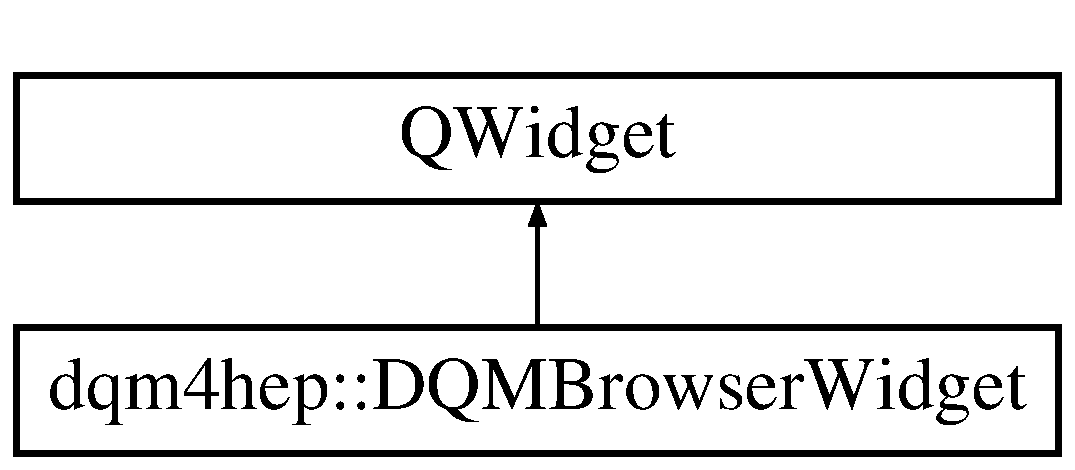
\includegraphics[height=2.000000cm]{classdqm4hep_1_1DQMBrowserWidget}
\end{center}
\end{figure}
\subsection*{Public Slots}
\begin{DoxyCompactItemize}
\item 
void {\bf update\+Collector\+List} ()
\begin{DoxyCompactList}\small\item\em Update the collector list (combo box) \end{DoxyCompactList}\end{DoxyCompactItemize}
\subsection*{Signals}
\begin{DoxyCompactItemize}
\item 
void {\bf key\+Press\+Event} (Q\+Key\+Event $\ast$)
\begin{DoxyCompactList}\small\item\em Key pressed event emitted in the tree widget. \end{DoxyCompactList}\end{DoxyCompactItemize}
\subsection*{Public Member Functions}
\begin{DoxyCompactItemize}
\item 
{\bf D\+Q\+M\+Browser\+Widget} ({\bf D\+Q\+M\+Monitoring} $\ast$p\+Monitoring)
\begin{DoxyCompactList}\small\item\em Constructor. \end{DoxyCompactList}\item 
{\bf $\sim$\+D\+Q\+M\+Browser\+Widget} ()
\begin{DoxyCompactList}\small\item\em Destructor. \end{DoxyCompactList}\item 
{\bf D\+Q\+M\+Monitoring} $\ast$ {\bf get\+Monitoring} () const 
\begin{DoxyCompactList}\small\item\em Get the monitoring instance. \end{DoxyCompactList}\item 
Q\+String {\bf get\+Collector\+Name} () const 
\begin{DoxyCompactList}\small\item\em Get the collector name. \end{DoxyCompactList}\end{DoxyCompactItemize}
\subsection*{Private Slots}
\begin{DoxyCompactItemize}
\item 
void {\bf handle\+Collector\+Selection} (int index)
\item 
void {\bf query\+Search} ()
\begin{DoxyCompactList}\small\item\em Send the query for monitor element browsing on the collector. \end{DoxyCompactList}\item 
void {\bf clear\+Search} ()
\begin{DoxyCompactList}\small\item\em Clear the search interface. \end{DoxyCompactList}\item 
void {\bf fill\+Module\+Name\+List} (const D\+Q\+M\+Monitor\+Element\+Info\+List \&name\+List)
\begin{DoxyCompactList}\small\item\em Fill the module name list. \end{DoxyCompactList}\item 
void {\bf check\+Item} (Q\+Tree\+Widget\+Item $\ast$p\+Item, int)
\begin{DoxyCompactList}\small\item\em Check/uncheck the given item. \end{DoxyCompactList}\item 
void {\bf check\+Selected\+Elements} ()
\begin{DoxyCompactList}\small\item\em Check all the selected items. \end{DoxyCompactList}\item 
void {\bf handle\+Key\+Press\+Event} (Q\+Key\+Event $\ast$p\+Key\+Event)
\begin{DoxyCompactList}\small\item\em Handle the key press event. \end{DoxyCompactList}\item 
void {\bf select\+All\+Elements} ()
\begin{DoxyCompactList}\small\item\em Select all items. \end{DoxyCompactList}\item 
void {\bf handle\+Update\+Button\+Clicked} ()
\item 
void {\bf handle\+Replace\+Button\+Clicked} ()
\end{DoxyCompactItemize}
\subsection*{Private Member Functions}
\begin{DoxyCompactItemize}
\item 
void {\bf build\+Monitor\+Element\+Info\+List} (D\+Q\+M\+Monitor\+Element\+Info\+List \&info\+List) const 
\begin{DoxyCompactList}\small\item\em Build the monitor element info list of the current selection. \end{DoxyCompactList}\end{DoxyCompactItemize}
\subsection*{Private Attributes}
\begin{DoxyCompactItemize}
\item 
{\bf D\+Q\+M\+Monitoring} $\ast$ {\bf m\+\_\+p\+Monitoring}
\item 
Q\+Combo\+Box $\ast$ {\bf m\+\_\+p\+Collector\+Name\+Combo\+Box}
\item 
Q\+Line\+Edit $\ast$ {\bf m\+\_\+p\+Module\+Name\+Edit}
\item 
Q\+Line\+Edit $\ast$ {\bf m\+\_\+p\+Monitor\+Element\+Name\+Edit}
\item 
Q\+Combo\+Box $\ast$ {\bf m\+\_\+p\+Monitor\+Element\+Type\+Combo\+Box}
\item 
Q\+Tree\+Widget $\ast$ {\bf m\+\_\+p\+Search\+Tree\+Widget}
\item 
Q\+Group\+Box $\ast$ {\bf m\+\_\+p\+Option\+Group\+Box}
\item 
Q\+Push\+Button $\ast$ {\bf m\+\_\+p\+Replace\+Button}
\item 
Q\+Push\+Button $\ast$ {\bf m\+\_\+p\+Append\+Button}
\item 
Q\+Push\+Button $\ast$ {\bf m\+\_\+p\+Close\+Button}
\item 
{\bf D\+Q\+M\+Gui\+Monitor\+Element\+Client} $\ast$ {\bf m\+\_\+p\+Monitor\+Element\+Client}
\end{DoxyCompactItemize}


\subsection{Detailed Description}
\doxyref{D\+Q\+M\+Browser\+Widget}{p.}{classdqm4hep_1_1DQMBrowserWidget} class. 

A browser to find monitor elements over the network. Uses a Dim\+Browser to perform the service finding, a monitor element client as the interface to the server and a qt handler for request call back functions received by the server. 

Definition at line 58 of file D\+Q\+M\+Browser\+Widget.\+h.



\subsection{Constructor \& Destructor Documentation}
\index{dqm4hep\+::\+D\+Q\+M\+Browser\+Widget@{dqm4hep\+::\+D\+Q\+M\+Browser\+Widget}!D\+Q\+M\+Browser\+Widget@{D\+Q\+M\+Browser\+Widget}}
\index{D\+Q\+M\+Browser\+Widget@{D\+Q\+M\+Browser\+Widget}!dqm4hep\+::\+D\+Q\+M\+Browser\+Widget@{dqm4hep\+::\+D\+Q\+M\+Browser\+Widget}}
\subsubsection[{D\+Q\+M\+Browser\+Widget}]{\setlength{\rightskip}{0pt plus 5cm}dqm4hep\+::\+D\+Q\+M\+Browser\+Widget\+::\+D\+Q\+M\+Browser\+Widget (
\begin{DoxyParamCaption}
\item[{{\bf D\+Q\+M\+Monitoring} $\ast$}]{p\+Monitoring}
\end{DoxyParamCaption}
)}\label{classdqm4hep_1_1DQMBrowserWidget_a4406e30b8d4bd73573edfb3672e818fd}


Constructor. 



Definition at line 55 of file D\+Q\+M\+Browser\+Widget.\+cc.



References check\+Item(), clear\+Search(), handle\+Collector\+Selection(), handle\+Key\+Press\+Event(), handle\+Replace\+Button\+Clicked(), handle\+Update\+Button\+Clicked(), key\+Press\+Event(), m\+\_\+p\+Append\+Button, m\+\_\+p\+Close\+Button, m\+\_\+p\+Collector\+Name\+Combo\+Box, m\+\_\+p\+Module\+Name\+Edit, m\+\_\+p\+Monitor\+Element\+Name\+Edit, m\+\_\+p\+Monitor\+Element\+Type\+Combo\+Box, m\+\_\+p\+Option\+Group\+Box, m\+\_\+p\+Replace\+Button, m\+\_\+p\+Search\+Tree\+Widget, query\+Search(), and update\+Collector\+List().


\begin{DoxyCode}
55                                                              :
56     QWidget(0),
57     m_pMonitoring(pMonitoring),
58     m_pMonitorElementClient(NULL)
59 \{
60   setLayout(\textcolor{keyword}{new} QVBoxLayout());
61 
62   \textcolor{keywordtype}{char} *pDnsNode = getenv(\textcolor{stringliteral}{"DIM\_DNS\_NODE"});
63   QString dimDnsNode = pDnsNode == NULL ? \textcolor{stringliteral}{"UNKNOWN"} : pDnsNode;
64 
65   \textcolor{comment}{// monitor element collector}
66   QGroupBox *pCollectorGroupBox = \textcolor{keyword}{new} QGroupBox(\textcolor{stringliteral}{"Monitor element collectors (DIM\_DNS\_NODE = "} + dimDnsNode 
      + \textcolor{stringliteral}{")"});
67   QFormLayout *pCollectorLayout = \textcolor{keyword}{new} QFormLayout();
68   pCollectorGroupBox->setLayout(pCollectorLayout);
69   layout()->addWidget(pCollectorGroupBox);
70 
71   QWidget *pCollectorNameWidget = \textcolor{keyword}{new} QWidget();
72   QHBoxLayout *pCollectorNameLayout = \textcolor{keyword}{new} QHBoxLayout();
73   pCollectorNameWidget->setLayout(pCollectorNameLayout);
74   pCollectorLayout->addRow(\textcolor{stringliteral}{"Monitor element collector : "}, pCollectorNameWidget);
75   m_pCollectorNameComboBox = \textcolor{keyword}{new} QComboBox();
76   pCollectorNameLayout->addWidget(m_pCollectorNameComboBox);
77   QPushButton *pUpdateCollectorListButton = \textcolor{keyword}{new} QPushButton(\textcolor{stringliteral}{"Update list"});
78   pUpdateCollectorListButton->setMaximumWidth(150);
79   pCollectorNameLayout->addWidget(pUpdateCollectorListButton);
80 
81   \textcolor{comment}{// search options with form and buttons}
82   m_pOptionGroupBox = \textcolor{keyword}{new} QGroupBox(\textcolor{stringliteral}{"Search option"}, \textcolor{keyword}{this});
83   QFormLayout *pOptionFormLayout = \textcolor{keyword}{new} QFormLayout();
84   m_pOptionGroupBox->setLayout(pOptionFormLayout);
85   m_pModuleNameEdit = \textcolor{keyword}{new} QLineEdit();
86   pOptionFormLayout->addRow(\textcolor{stringliteral}{"Module name"}, m_pModuleNameEdit);
87   m_pMonitorElementNameEdit = \textcolor{keyword}{new} QLineEdit();
88   pOptionFormLayout->addRow(\textcolor{stringliteral}{"Monitor element name"}, m_pMonitorElementNameEdit);
89   m_pMonitorElementTypeComboBox = \textcolor{keyword}{new} QComboBox();
90   m_pMonitorElementTypeComboBox->addItem(\textcolor{stringliteral}{"All"}, NO\_ELEMENT\_TYPE);
91   m_pMonitorElementTypeComboBox->addItem(monitorElementTypeToString(INT\_ELEMENT\_TYPE).c\_str(), 
      INT\_ELEMENT\_TYPE);
92   m_pMonitorElementTypeComboBox->addItem(monitorElementTypeToString(REAL\_ELEMENT\_TYPE).c\_str(), 
      REAL\_ELEMENT\_TYPE);
93   m_pMonitorElementTypeComboBox->addItem(monitorElementTypeToString(SHORT\_ELEMENT\_TYPE).c\_str(), 
      SHORT\_ELEMENT\_TYPE);
94   m_pMonitorElementTypeComboBox->addItem(monitorElementTypeToString(STRING\_ELEMENT\_TYPE).c\_str(), 
      STRING\_ELEMENT\_TYPE);
95   m_pMonitorElementTypeComboBox->addItem(monitorElementTypeToString(INT\_HISTOGRAM\_1D\_ELEMENT\_TYPE).c\_str(),
       INT\_HISTOGRAM\_1D\_ELEMENT\_TYPE);
96   m_pMonitorElementTypeComboBox->addItem(monitorElementTypeToString(REAL\_HISTOGRAM\_1D\_ELEMENT\_TYPE).c\_str()
      , REAL\_HISTOGRAM\_1D\_ELEMENT\_TYPE);
97   m_pMonitorElementTypeComboBox->addItem(monitorElementTypeToString(SHORT\_HISTOGRAM\_1D\_ELEMENT\_TYPE).c\_str(
      ), SHORT\_HISTOGRAM\_1D\_ELEMENT\_TYPE);
98   m_pMonitorElementTypeComboBox->addItem(monitorElementTypeToString(CHAR\_HISTOGRAM\_1D\_ELEMENT\_TYPE).c\_str()
      , CHAR\_HISTOGRAM\_1D\_ELEMENT\_TYPE);
99   m_pMonitorElementTypeComboBox->addItem(monitorElementTypeToString(INT\_HISTOGRAM\_2D\_ELEMENT\_TYPE).c\_str(),
       INT\_HISTOGRAM\_2D\_ELEMENT\_TYPE);
100   m_pMonitorElementTypeComboBox->addItem(monitorElementTypeToString(REAL\_HISTOGRAM\_2D\_ELEMENT\_TYPE).c\_str()
      , REAL\_HISTOGRAM\_2D\_ELEMENT\_TYPE);
101   m_pMonitorElementTypeComboBox->addItem(monitorElementTypeToString(CHAR\_HISTOGRAM\_2D\_ELEMENT\_TYPE).c\_str()
      , CHAR\_HISTOGRAM\_2D\_ELEMENT\_TYPE);
102   m_pMonitorElementTypeComboBox->addItem(monitorElementTypeToString(SHORT\_HISTOGRAM\_2D\_ELEMENT\_TYPE).c\_str(
      ), SHORT\_HISTOGRAM\_2D\_ELEMENT\_TYPE);
103   m_pMonitorElementTypeComboBox->addItem(monitorElementTypeToString(PROFILE\_1D\_ELEMENT\_TYPE).c\_str(), 
      PROFILE\_1D\_ELEMENT\_TYPE);
104   m_pMonitorElementTypeComboBox->addItem(monitorElementTypeToString(PROFILE\_2D\_ELEMENT\_TYPE).c\_str(), 
      PROFILE\_2D\_ELEMENT\_TYPE);
105   pOptionFormLayout->addRow(\textcolor{stringliteral}{"Monitor element type"}, 
      m_pMonitorElementTypeComboBox);
106   QWidget *pSearchButtonAreaWidget = \textcolor{keyword}{new} QWidget();
107   pOptionFormLayout->addRow(\textcolor{stringliteral}{""}, pSearchButtonAreaWidget);
108   QHBoxLayout *pSearchAreaLayout = \textcolor{keyword}{new} QHBoxLayout();
109   pSearchButtonAreaWidget->setLayout(pSearchAreaLayout);
110   QPushButton *pStartSearchButton = \textcolor{keyword}{new} QPushButton(\textcolor{stringliteral}{"Search"});
111   pStartSearchButton->setMaximumWidth(150);
112   pSearchAreaLayout->addWidget(pStartSearchButton);
113   QPushButton *pClearSelectionButton = \textcolor{keyword}{new} QPushButton(\textcolor{stringliteral}{"Clear"});
114   pClearSelectionButton->setMaximumWidth(150);
115   pSearchAreaLayout->addWidget(pClearSelectionButton);
116   layout()->addWidget(m_pOptionGroupBox);
117 
118   \textcolor{comment}{// search result main view}
119   QGroupBox *pSearchResultGroupBox = \textcolor{keyword}{new} QGroupBox(\textcolor{stringliteral}{"Search result"});
120   layout()->addWidget(pSearchResultGroupBox);
121   QHBoxLayout *pSearchResultLayout = \textcolor{keyword}{new} QHBoxLayout();
122   pSearchResultGroupBox->setLayout(pSearchResultLayout);
123   m_pSearchTreeWidget = \textcolor{keyword}{new} QTreeWidget();
124   m_pSearchTreeWidget->setHeaderLabels(QStringList() << \textcolor{stringliteral}{"Module"} << \textcolor{stringliteral}{"Directory"} << \textcolor{stringliteral}{"Name"} << \textcolor{stringliteral}{"Type"});
125   pSearchResultLayout->addWidget(m_pSearchTreeWidget);
126 
127   \textcolor{comment}{// bottom button area}
128   QWidget *pBottomButtonAreaWidget = \textcolor{keyword}{new} QWidget();
129   layout()->addWidget(pBottomButtonAreaWidget);
130   QHBoxLayout *pBottomAreaLayout = \textcolor{keyword}{new} QHBoxLayout();
131   pBottomButtonAreaWidget->setLayout(pBottomAreaLayout);
132 
133   m_pReplaceButton = \textcolor{keyword}{new} QPushButton(\textcolor{stringliteral}{"Replace"});
134   m_pReplaceButton->setMaximumWidth(150);
135   m_pReplaceButton->setEnabled(\textcolor{keyword}{false});
136   pBottomAreaLayout->addWidget(m_pReplaceButton);
137 
138   m_pAppendButton = \textcolor{keyword}{new} QPushButton(\textcolor{stringliteral}{"Append"});
139   m_pAppendButton->setMaximumWidth(150);
140   m_pAppendButton->setEnabled(\textcolor{keyword}{false});
141   pBottomAreaLayout->addWidget(m_pAppendButton);
142 
143   m_pCloseButton = \textcolor{keyword}{new} QPushButton(\textcolor{stringliteral}{"Close"});
144   m_pCloseButton->setMaximumWidth(150);
145   pBottomAreaLayout->addWidget(m_pCloseButton);
146 
147   connect(m_pCloseButton, SIGNAL(clicked()), \textcolor{keyword}{this}, SLOT(close()));
148   connect(pUpdateCollectorListButton, SIGNAL(clicked()), \textcolor{keyword}{this}, SLOT(
      updateCollectorList()));
149 
150   connect(m_pCollectorNameComboBox, SIGNAL(currentIndexChanged(\textcolor{keywordtype}{int})), \textcolor{keyword}{this}, SLOT(
      handleCollectorSelection(\textcolor{keywordtype}{int})));
151   connect(pClearSelectionButton, SIGNAL(clicked()), \textcolor{keyword}{this}, SLOT(clearSearch()));
152   connect(pStartSearchButton, SIGNAL(clicked()), \textcolor{keyword}{this}, SLOT(querySearch()));
153   connect(m_pSearchTreeWidget, SIGNAL(itemDoubleClicked(QTreeWidgetItem *, \textcolor{keywordtype}{int})), \textcolor{keyword}{this}, SLOT(
      checkItem(QTreeWidgetItem*, \textcolor{keywordtype}{int})));
154   connect(\textcolor{keyword}{this}, SIGNAL(keyPressEvent(QKeyEvent*)), \textcolor{keyword}{this}, SLOT(
      handleKeyPressEvent(QKeyEvent*)));
155   connect(m_pAppendButton, SIGNAL(clicked()), \textcolor{keyword}{this}, SLOT(
      handleUpdateButtonClicked()));
156   connect(m_pReplaceButton, SIGNAL(clicked()), \textcolor{keyword}{this}, SLOT(
      handleReplaceButtonClicked()));
157 
158   updateCollectorList();
159 
160   resize(700, 700);
161 \}
\end{DoxyCode}
\index{dqm4hep\+::\+D\+Q\+M\+Browser\+Widget@{dqm4hep\+::\+D\+Q\+M\+Browser\+Widget}!````~D\+Q\+M\+Browser\+Widget@{$\sim$\+D\+Q\+M\+Browser\+Widget}}
\index{````~D\+Q\+M\+Browser\+Widget@{$\sim$\+D\+Q\+M\+Browser\+Widget}!dqm4hep\+::\+D\+Q\+M\+Browser\+Widget@{dqm4hep\+::\+D\+Q\+M\+Browser\+Widget}}
\subsubsection[{$\sim$\+D\+Q\+M\+Browser\+Widget}]{\setlength{\rightskip}{0pt plus 5cm}dqm4hep\+::\+D\+Q\+M\+Browser\+Widget\+::$\sim$\+D\+Q\+M\+Browser\+Widget (
\begin{DoxyParamCaption}
{}
\end{DoxyParamCaption}
)}\label{classdqm4hep_1_1DQMBrowserWidget_ac5d62dc4a89aa1d7304a7330d4836fd5}


Destructor. 



Definition at line 165 of file D\+Q\+M\+Browser\+Widget.\+cc.



References m\+\_\+p\+Monitor\+Element\+Client.


\begin{DoxyCode}
166 \{
167   \textcolor{keywordflow}{if}(m_pMonitorElementClient)
168     m_pMonitorElementClient->deleteLater();
169 \}
\end{DoxyCode}


\subsection{Member Function Documentation}
\index{dqm4hep\+::\+D\+Q\+M\+Browser\+Widget@{dqm4hep\+::\+D\+Q\+M\+Browser\+Widget}!build\+Monitor\+Element\+Info\+List@{build\+Monitor\+Element\+Info\+List}}
\index{build\+Monitor\+Element\+Info\+List@{build\+Monitor\+Element\+Info\+List}!dqm4hep\+::\+D\+Q\+M\+Browser\+Widget@{dqm4hep\+::\+D\+Q\+M\+Browser\+Widget}}
\subsubsection[{build\+Monitor\+Element\+Info\+List}]{\setlength{\rightskip}{0pt plus 5cm}void dqm4hep\+::\+D\+Q\+M\+Browser\+Widget\+::build\+Monitor\+Element\+Info\+List (
\begin{DoxyParamCaption}
\item[{D\+Q\+M\+Monitor\+Element\+Info\+List \&}]{info\+List}
\end{DoxyParamCaption}
) const\hspace{0.3cm}{\ttfamily [private]}}\label{classdqm4hep_1_1DQMBrowserWidget_a6c3246d59774f957c42b4f4f403b8bd9}


Build the monitor element info list of the current selection. 



Definition at line 384 of file D\+Q\+M\+Browser\+Widget.\+cc.



References m\+\_\+p\+Search\+Tree\+Widget.



Referenced by handle\+Replace\+Button\+Clicked(), and handle\+Update\+Button\+Clicked().


\begin{DoxyCode}
385 \{
386   \textcolor{keywordflow}{for}(\textcolor{keywordtype}{unsigned} \textcolor{keywordtype}{int} i=0 ; i<m_pSearchTreeWidget->topLevelItemCount() ; i++)
387   \{
388     \textcolor{keywordflow}{if}(Qt::Checked == m_pSearchTreeWidget->topLevelItem(i)->checkState(0))
389     \{
390       DQMMonitorElementInfo info;
391 
392       info.m\_moduleName = m_pSearchTreeWidget->topLevelItem(i)->text(0).toStdString();
393       info.m\_monitorElementFullPath = m_pSearchTreeWidget->topLevelItem(i)->text(1).toStdString();
394       info.m\_monitorElementName = m_pSearchTreeWidget->topLevelItem(i)->text(2).toStdString();
395       info.m\_monitorElementType = m_pSearchTreeWidget->topLevelItem(i)->text(3).toStdString();
396       info.m\_monitorElementDescription = m_pSearchTreeWidget->topLevelItem(i)->toolTip(0).toStdString();
397 
398       infoList.push\_back(info);
399     \}
400   \}
401 \}
\end{DoxyCode}
\index{dqm4hep\+::\+D\+Q\+M\+Browser\+Widget@{dqm4hep\+::\+D\+Q\+M\+Browser\+Widget}!check\+Item@{check\+Item}}
\index{check\+Item@{check\+Item}!dqm4hep\+::\+D\+Q\+M\+Browser\+Widget@{dqm4hep\+::\+D\+Q\+M\+Browser\+Widget}}
\subsubsection[{check\+Item}]{\setlength{\rightskip}{0pt plus 5cm}void dqm4hep\+::\+D\+Q\+M\+Browser\+Widget\+::check\+Item (
\begin{DoxyParamCaption}
\item[{Q\+Tree\+Widget\+Item $\ast$}]{p\+Item, }
\item[{int}]{}
\end{DoxyParamCaption}
)\hspace{0.3cm}{\ttfamily [private]}, {\ttfamily [slot]}}\label{classdqm4hep_1_1DQMBrowserWidget_a8580a0179efc06b6abd93f132d3984e0}


Check/uncheck the given item. 



Definition at line 332 of file D\+Q\+M\+Browser\+Widget.\+cc.



Referenced by D\+Q\+M\+Browser\+Widget().


\begin{DoxyCode}
333 \{
334   Qt::CheckState state = pItem->checkState(0);
335   pItem->setCheckState(0, state == Qt::Checked ? Qt::Unchecked : Qt::Checked);
336 \}
\end{DoxyCode}
\index{dqm4hep\+::\+D\+Q\+M\+Browser\+Widget@{dqm4hep\+::\+D\+Q\+M\+Browser\+Widget}!check\+Selected\+Elements@{check\+Selected\+Elements}}
\index{check\+Selected\+Elements@{check\+Selected\+Elements}!dqm4hep\+::\+D\+Q\+M\+Browser\+Widget@{dqm4hep\+::\+D\+Q\+M\+Browser\+Widget}}
\subsubsection[{check\+Selected\+Elements}]{\setlength{\rightskip}{0pt plus 5cm}void dqm4hep\+::\+D\+Q\+M\+Browser\+Widget\+::check\+Selected\+Elements (
\begin{DoxyParamCaption}
{}
\end{DoxyParamCaption}
)\hspace{0.3cm}{\ttfamily [private]}, {\ttfamily [slot]}}\label{classdqm4hep_1_1DQMBrowserWidget_abdc1d55fe66b90d63d84797d3f0916eb}


Check all the selected items. 



Definition at line 350 of file D\+Q\+M\+Browser\+Widget.\+cc.



References m\+\_\+p\+Search\+Tree\+Widget.



Referenced by handle\+Key\+Press\+Event().


\begin{DoxyCode}
351 \{
352   QList<QTreeWidgetItem *> selectedItems = m_pSearchTreeWidget->selectedItems();
353 
354   \textcolor{keywordflow}{if}(selectedItems.isEmpty())
355     \textcolor{keywordflow}{return};
356 
357   Qt::CheckState state = Qt::Checked;
358 
359   \textcolor{keywordflow}{for}(\textcolor{keywordtype}{unsigned} \textcolor{keywordtype}{int} i=0 ; i<selectedItems.size() ; i++)
360   \{
361     \textcolor{keywordflow}{if}(i == 0)
362     \{
363       QTreeWidgetItem *pFirstItem = selectedItems.at(i);
364 
365       \textcolor{keywordflow}{if}(pFirstItem->checkState(0) == Qt::Checked)
366         state = Qt::Unchecked;
367     \}
368 
369     QTreeWidgetItem *pItem = selectedItems.at(i);
370     pItem->setCheckState(0, state);
371   \}
372 \}
\end{DoxyCode}
\index{dqm4hep\+::\+D\+Q\+M\+Browser\+Widget@{dqm4hep\+::\+D\+Q\+M\+Browser\+Widget}!clear\+Search@{clear\+Search}}
\index{clear\+Search@{clear\+Search}!dqm4hep\+::\+D\+Q\+M\+Browser\+Widget@{dqm4hep\+::\+D\+Q\+M\+Browser\+Widget}}
\subsubsection[{clear\+Search}]{\setlength{\rightskip}{0pt plus 5cm}void dqm4hep\+::\+D\+Q\+M\+Browser\+Widget\+::clear\+Search (
\begin{DoxyParamCaption}
{}
\end{DoxyParamCaption}
)\hspace{0.3cm}{\ttfamily [private]}, {\ttfamily [slot]}}\label{classdqm4hep_1_1DQMBrowserWidget_aaec84c952b61584e4179ccb65dc755c4}


Clear the search interface. 



Definition at line 273 of file D\+Q\+M\+Browser\+Widget.\+cc.



References m\+\_\+p\+Module\+Name\+Edit, m\+\_\+p\+Monitor\+Element\+Name\+Edit, m\+\_\+p\+Monitor\+Element\+Type\+Combo\+Box, and m\+\_\+p\+Search\+Tree\+Widget.



Referenced by D\+Q\+M\+Browser\+Widget(), handle\+Collector\+Selection(), and update\+Collector\+List().


\begin{DoxyCode}
274 \{
275   m_pModuleNameEdit->clear();
276   m_pMonitorElementNameEdit->clear();
277   m_pMonitorElementTypeComboBox->setCurrentIndex(0);
278   m_pSearchTreeWidget->clear();
279 \}
\end{DoxyCode}
\index{dqm4hep\+::\+D\+Q\+M\+Browser\+Widget@{dqm4hep\+::\+D\+Q\+M\+Browser\+Widget}!fill\+Module\+Name\+List@{fill\+Module\+Name\+List}}
\index{fill\+Module\+Name\+List@{fill\+Module\+Name\+List}!dqm4hep\+::\+D\+Q\+M\+Browser\+Widget@{dqm4hep\+::\+D\+Q\+M\+Browser\+Widget}}
\subsubsection[{fill\+Module\+Name\+List}]{\setlength{\rightskip}{0pt plus 5cm}void dqm4hep\+::\+D\+Q\+M\+Browser\+Widget\+::fill\+Module\+Name\+List (
\begin{DoxyParamCaption}
\item[{const D\+Q\+M\+Monitor\+Element\+Info\+List \&}]{name\+List}
\end{DoxyParamCaption}
)\hspace{0.3cm}{\ttfamily [private]}, {\ttfamily [slot]}}\label{classdqm4hep_1_1DQMBrowserWidget_a2adda23c93a75cf8e52e73ec7d9f75a4}


Fill the module name list. 



Definition at line 298 of file D\+Q\+M\+Browser\+Widget.\+cc.



References m\+\_\+p\+Search\+Tree\+Widget.



Referenced by handle\+Collector\+Selection().


\begin{DoxyCode}
299 \{
300   m_pSearchTreeWidget->clear();
301 
302   \textcolor{keywordflow}{if}(nameList.empty())
303     \textcolor{keywordflow}{return};
304 
305   \textcolor{keywordflow}{for}(\textcolor{keywordtype}{unsigned} \textcolor{keywordtype}{int} i=0 ; i<nameList.size() ; i++)
306   \{
307     QString moduleName = nameList.at(i).m\_moduleName.c\_str();
308     QString monitorElementFullPath = nameList.at(i).m\_monitorElementFullPath.c\_str();
309     QString monitorElementName = nameList.at(i).m\_monitorElementName.c\_str();
310     QString monitorElementType = nameList.at(i).m\_monitorElementType.c\_str();
311     QString monitorElementDescription = nameList.at(i).m\_monitorElementDescription.c\_str();
312 
313     QStringList itemColumns;
314     itemColumns << moduleName << monitorElementFullPath << monitorElementName << monitorElementType;
315 
316     QTreeWidgetItem *pItem = \textcolor{keyword}{new} QTreeWidgetItem(itemColumns);
317 
318     pItem->setCheckState(0, Qt::Checked);
319     pItem->setToolTip(0, monitorElementDescription);
320     pItem->setToolTip(1, monitorElementDescription);
321     pItem->setToolTip(2, monitorElementDescription);
322     pItem->setToolTip(3, monitorElementDescription);
323 
324     m_pSearchTreeWidget->addTopLevelItem(pItem);
325   \}
326 
327   m_pSearchTreeWidget->header()->resizeSections(QHeaderView::Stretch);
328 \}
\end{DoxyCode}
\index{dqm4hep\+::\+D\+Q\+M\+Browser\+Widget@{dqm4hep\+::\+D\+Q\+M\+Browser\+Widget}!get\+Collector\+Name@{get\+Collector\+Name}}
\index{get\+Collector\+Name@{get\+Collector\+Name}!dqm4hep\+::\+D\+Q\+M\+Browser\+Widget@{dqm4hep\+::\+D\+Q\+M\+Browser\+Widget}}
\subsubsection[{get\+Collector\+Name}]{\setlength{\rightskip}{0pt plus 5cm}Q\+String dqm4hep\+::\+D\+Q\+M\+Browser\+Widget\+::get\+Collector\+Name (
\begin{DoxyParamCaption}
{}
\end{DoxyParamCaption}
) const}\label{classdqm4hep_1_1DQMBrowserWidget_a730ffbb078275be046d612caa8a62a09}


Get the collector name. 



Definition at line 180 of file D\+Q\+M\+Browser\+Widget.\+cc.



References m\+\_\+p\+Collector\+Name\+Combo\+Box.



Referenced by handle\+Replace\+Button\+Clicked(), handle\+Update\+Button\+Clicked(), and update\+Collector\+List().


\begin{DoxyCode}
181 \{
182   \textcolor{keywordflow}{if}(m_pCollectorNameComboBox->currentIndex() != 0)
183     \textcolor{keywordflow}{return} m_pCollectorNameComboBox->currentText();
184 
185   \textcolor{keywordflow}{return} QString();
186 \}
\end{DoxyCode}
\index{dqm4hep\+::\+D\+Q\+M\+Browser\+Widget@{dqm4hep\+::\+D\+Q\+M\+Browser\+Widget}!get\+Monitoring@{get\+Monitoring}}
\index{get\+Monitoring@{get\+Monitoring}!dqm4hep\+::\+D\+Q\+M\+Browser\+Widget@{dqm4hep\+::\+D\+Q\+M\+Browser\+Widget}}
\subsubsection[{get\+Monitoring}]{\setlength{\rightskip}{0pt plus 5cm}{\bf D\+Q\+M\+Monitoring} $\ast$ dqm4hep\+::\+D\+Q\+M\+Browser\+Widget\+::get\+Monitoring (
\begin{DoxyParamCaption}
{}
\end{DoxyParamCaption}
) const}\label{classdqm4hep_1_1DQMBrowserWidget_a5c969f26b48a5c5c63ae5aa202faabf2}


Get the monitoring instance. 



Definition at line 173 of file D\+Q\+M\+Browser\+Widget.\+cc.



References m\+\_\+p\+Monitoring.



Referenced by handle\+Collector\+Selection(), handle\+Replace\+Button\+Clicked(), and handle\+Update\+Button\+Clicked().


\begin{DoxyCode}
174 \{
175   \textcolor{keywordflow}{return} m_pMonitoring;
176 \}
\end{DoxyCode}
\index{dqm4hep\+::\+D\+Q\+M\+Browser\+Widget@{dqm4hep\+::\+D\+Q\+M\+Browser\+Widget}!handle\+Collector\+Selection@{handle\+Collector\+Selection}}
\index{handle\+Collector\+Selection@{handle\+Collector\+Selection}!dqm4hep\+::\+D\+Q\+M\+Browser\+Widget@{dqm4hep\+::\+D\+Q\+M\+Browser\+Widget}}
\subsubsection[{handle\+Collector\+Selection}]{\setlength{\rightskip}{0pt plus 5cm}void dqm4hep\+::\+D\+Q\+M\+Browser\+Widget\+::handle\+Collector\+Selection (
\begin{DoxyParamCaption}
\item[{int}]{index}
\end{DoxyParamCaption}
)\hspace{0.3cm}{\ttfamily [private]}, {\ttfamily [slot]}}\label{classdqm4hep_1_1DQMBrowserWidget_a9b5482b0637abd55d602530ff67de4ad}


Definition at line 217 of file D\+Q\+M\+Browser\+Widget.\+cc.



References clear\+Search(), dqm4hep\+::\+D\+Q\+M\+Monitoring\+Controller\+::create\+Client(), fill\+Module\+Name\+List(), dqm4hep\+::\+D\+Q\+M\+Monitoring\+::get\+Controller(), dqm4hep\+::\+D\+Q\+M\+Gui\+Monitor\+Element\+Client\+::get\+Monitor\+Element\+Client(), get\+Monitoring(), m\+\_\+p\+Append\+Button, m\+\_\+p\+Collector\+Name\+Combo\+Box, m\+\_\+p\+Monitor\+Element\+Client, m\+\_\+p\+Replace\+Button, and query\+Search().



Referenced by D\+Q\+M\+Browser\+Widget().


\begin{DoxyCode}
218 \{
219   \textcolor{keywordflow}{if}(index < 0)
220     \textcolor{keywordflow}{return};
221 
222   \textcolor{keywordflow}{if}(index == 0)
223   \{
224     clearSearch();
225 
226     \textcolor{keywordflow}{if}(m_pMonitorElementClient)
227     \{
228       m_pMonitorElementClient->deleteLater();
229       m_pMonitorElementClient = 0;
230     \}
231 
232     m_pReplaceButton->setEnabled(\textcolor{keyword}{false});
233     m_pAppendButton->setEnabled(\textcolor{keyword}{false});
234 
235     \textcolor{keywordflow}{return};
236   \}
237 
238   m_pReplaceButton->setEnabled(\textcolor{keyword}{true});
239   m_pAppendButton->setEnabled(\textcolor{keyword}{true});
240 
241   QString newCollectorName = m_pCollectorNameComboBox->itemText(index);
242 
243   \textcolor{keywordflow}{if}(m_pMonitorElementClient)
244   \{
245     \textcolor{keywordtype}{bool} sameCollectorName =
246         newCollectorName.toStdString()
247         ==
248         m_pMonitorElementClient->getMonitorElementClient()->getCollectorName();
249 
250     \textcolor{keywordflow}{if}(!sameCollectorName)
251     \{
252       m_pMonitorElementClient->deleteLater();
253       m_pMonitorElementClient = 0;
254     \}
255   \}
256 
257 
258   \textcolor{keywordflow}{if}(!m_pMonitorElementClient)
259   \{
260     m_pMonitorElementClient = this->getMonitoring()->getController()->
      createClient(newCollectorName.toStdString());
261     m_pMonitorElementClient->getMonitorElementClient()->connectToService();
262 
263     connect(m_pMonitorElementClient, SIGNAL(monitorElementListNameReceived(\textcolor{keyword}{const} DQMMonitorElementInfoList 
      &)),
264         \textcolor{keyword}{this}, SLOT(fillModuleNameList(\textcolor{keyword}{const} DQMMonitorElementInfoList &)));
265 
266     clearSearch();
267     querySearch();
268   \}
269 \}
\end{DoxyCode}
\index{dqm4hep\+::\+D\+Q\+M\+Browser\+Widget@{dqm4hep\+::\+D\+Q\+M\+Browser\+Widget}!handle\+Key\+Press\+Event@{handle\+Key\+Press\+Event}}
\index{handle\+Key\+Press\+Event@{handle\+Key\+Press\+Event}!dqm4hep\+::\+D\+Q\+M\+Browser\+Widget@{dqm4hep\+::\+D\+Q\+M\+Browser\+Widget}}
\subsubsection[{handle\+Key\+Press\+Event}]{\setlength{\rightskip}{0pt plus 5cm}void dqm4hep\+::\+D\+Q\+M\+Browser\+Widget\+::handle\+Key\+Press\+Event (
\begin{DoxyParamCaption}
\item[{Q\+Key\+Event $\ast$}]{p\+Key\+Event}
\end{DoxyParamCaption}
)\hspace{0.3cm}{\ttfamily [private]}, {\ttfamily [slot]}}\label{classdqm4hep_1_1DQMBrowserWidget_aae8d192a53bbb61afef7b1eaea5c0cc6}


Handle the key press event. 


\begin{DoxyItemize}
\item Key Alt+\+A \+: select all elements in the list
\item Key enter \+: check all the selected items 
\end{DoxyItemize}

Definition at line 340 of file D\+Q\+M\+Browser\+Widget.\+cc.



References check\+Selected\+Elements(), and select\+All\+Elements().



Referenced by D\+Q\+M\+Browser\+Widget().


\begin{DoxyCode}
341 \{
342   \textcolor{keywordflow}{if}(pKeyEvent->key() == Qt::Key\_Return)
343     checkSelectedElements();
344   \textcolor{keywordflow}{if}(pKeyEvent->key() == Qt::Key\_A)
345     selectAllElements();
346 \}
\end{DoxyCode}
\index{dqm4hep\+::\+D\+Q\+M\+Browser\+Widget@{dqm4hep\+::\+D\+Q\+M\+Browser\+Widget}!handle\+Replace\+Button\+Clicked@{handle\+Replace\+Button\+Clicked}}
\index{handle\+Replace\+Button\+Clicked@{handle\+Replace\+Button\+Clicked}!dqm4hep\+::\+D\+Q\+M\+Browser\+Widget@{dqm4hep\+::\+D\+Q\+M\+Browser\+Widget}}
\subsubsection[{handle\+Replace\+Button\+Clicked}]{\setlength{\rightskip}{0pt plus 5cm}void dqm4hep\+::\+D\+Q\+M\+Browser\+Widget\+::handle\+Replace\+Button\+Clicked (
\begin{DoxyParamCaption}
{}
\end{DoxyParamCaption}
)\hspace{0.3cm}{\ttfamily [private]}, {\ttfamily [slot]}}\label{classdqm4hep_1_1DQMBrowserWidget_a57da030ef6f77229a57640e60fea277a}


Definition at line 424 of file D\+Q\+M\+Browser\+Widget.\+cc.



References build\+Monitor\+Element\+Info\+List(), dqm4hep\+::\+D\+Q\+M\+Monitoring\+Controller\+::clear\+View\+And\+Model(), dqm4hep\+::\+D\+Q\+M\+Monitoring\+Controller\+::create\+Empty\+Monitor\+Elements(), dqm4hep\+::\+D\+Q\+M\+Monitoring\+Controller\+::get\+Client(), get\+Collector\+Name(), dqm4hep\+::\+D\+Q\+M\+Monitoring\+::get\+Controller(), and get\+Monitoring().



Referenced by D\+Q\+M\+Browser\+Widget().


\begin{DoxyCode}
425 \{
426   DQMMonitorElementInfoList infoList;
427   this->buildMonitorElementInfoList(infoList);
428 
429   std::string collectorName = this->getCollectorName().toStdString();
430 
431   \textcolor{keywordflow}{if}(infoList.empty() || collectorName.empty())
432     \textcolor{keywordflow}{return};
433 
434   this->getMonitoring()->getController()->clearViewAndModel();
435 
436   \textcolor{comment}{// create the client instance (owned by the controller)}
437   this->getMonitoring()->getController()->getClient(collectorName);
438 
439   \textcolor{comment}{// create the list in view}
440   this->getMonitoring()->getController()->createEmptyMonitorElements(collectorName, infoList);
441 \}
\end{DoxyCode}
\index{dqm4hep\+::\+D\+Q\+M\+Browser\+Widget@{dqm4hep\+::\+D\+Q\+M\+Browser\+Widget}!handle\+Update\+Button\+Clicked@{handle\+Update\+Button\+Clicked}}
\index{handle\+Update\+Button\+Clicked@{handle\+Update\+Button\+Clicked}!dqm4hep\+::\+D\+Q\+M\+Browser\+Widget@{dqm4hep\+::\+D\+Q\+M\+Browser\+Widget}}
\subsubsection[{handle\+Update\+Button\+Clicked}]{\setlength{\rightskip}{0pt plus 5cm}void dqm4hep\+::\+D\+Q\+M\+Browser\+Widget\+::handle\+Update\+Button\+Clicked (
\begin{DoxyParamCaption}
{}
\end{DoxyParamCaption}
)\hspace{0.3cm}{\ttfamily [private]}, {\ttfamily [slot]}}\label{classdqm4hep_1_1DQMBrowserWidget_aa93a957f87377f6a91c354d6ce246273}


Definition at line 405 of file D\+Q\+M\+Browser\+Widget.\+cc.



References build\+Monitor\+Element\+Info\+List(), dqm4hep\+::\+D\+Q\+M\+Monitoring\+Controller\+::create\+Empty\+Monitor\+Elements(), dqm4hep\+::\+D\+Q\+M\+Monitoring\+Controller\+::get\+Client(), get\+Collector\+Name(), dqm4hep\+::\+D\+Q\+M\+Monitoring\+::get\+Controller(), and get\+Monitoring().



Referenced by D\+Q\+M\+Browser\+Widget().


\begin{DoxyCode}
406 \{
407   DQMMonitorElementInfoList infoList;
408   this->buildMonitorElementInfoList(infoList);
409 
410   std::string collectorName = this->getCollectorName().toStdString();
411 
412   \textcolor{keywordflow}{if}(infoList.empty() || collectorName.empty())
413     \textcolor{keywordflow}{return};
414 
415   \textcolor{comment}{// create the client instance (owned by the controller)}
416   this->getMonitoring()->getController()->getClient(collectorName);
417 
418   \textcolor{comment}{// create the list in view}
419   this->getMonitoring()->getController()->createEmptyMonitorElements(collectorName, infoList);
420 \}
\end{DoxyCode}
\index{dqm4hep\+::\+D\+Q\+M\+Browser\+Widget@{dqm4hep\+::\+D\+Q\+M\+Browser\+Widget}!key\+Press\+Event@{key\+Press\+Event}}
\index{key\+Press\+Event@{key\+Press\+Event}!dqm4hep\+::\+D\+Q\+M\+Browser\+Widget@{dqm4hep\+::\+D\+Q\+M\+Browser\+Widget}}
\subsubsection[{key\+Press\+Event}]{\setlength{\rightskip}{0pt plus 5cm}void dqm4hep\+::\+D\+Q\+M\+Browser\+Widget\+::key\+Press\+Event (
\begin{DoxyParamCaption}
\item[{Q\+Key\+Event $\ast$}]{}
\end{DoxyParamCaption}
)\hspace{0.3cm}{\ttfamily [signal]}}\label{classdqm4hep_1_1DQMBrowserWidget_a7f0671cef326a5ddc9f2ec2544152ce1}


Key pressed event emitted in the tree widget. 



Referenced by D\+Q\+M\+Browser\+Widget().

\index{dqm4hep\+::\+D\+Q\+M\+Browser\+Widget@{dqm4hep\+::\+D\+Q\+M\+Browser\+Widget}!query\+Search@{query\+Search}}
\index{query\+Search@{query\+Search}!dqm4hep\+::\+D\+Q\+M\+Browser\+Widget@{dqm4hep\+::\+D\+Q\+M\+Browser\+Widget}}
\subsubsection[{query\+Search}]{\setlength{\rightskip}{0pt plus 5cm}void dqm4hep\+::\+D\+Q\+M\+Browser\+Widget\+::query\+Search (
\begin{DoxyParamCaption}
{}
\end{DoxyParamCaption}
)\hspace{0.3cm}{\ttfamily [private]}, {\ttfamily [slot]}}\label{classdqm4hep_1_1DQMBrowserWidget_a3c1831ee701496212b291cae2a2e6811}


Send the query for monitor element browsing on the collector. 



Definition at line 283 of file D\+Q\+M\+Browser\+Widget.\+cc.



References dqm4hep\+::\+D\+Q\+M\+Gui\+Monitor\+Element\+Client\+::get\+Monitor\+Element\+Client(), m\+\_\+p\+Module\+Name\+Edit, m\+\_\+p\+Monitor\+Element\+Client, m\+\_\+p\+Monitor\+Element\+Name\+Edit, and m\+\_\+p\+Monitor\+Element\+Type\+Combo\+Box.



Referenced by D\+Q\+M\+Browser\+Widget(), and handle\+Collector\+Selection().


\begin{DoxyCode}
284 \{
285   \textcolor{keywordflow}{if}(!m_pMonitorElementClient)
286     \textcolor{keywordflow}{return};
287 
288   DQMMonitorElementListNameRequest request;
289   request.m\_moduleName = m_pModuleNameEdit->text().toStdString();
290   request.m\_monitorElementName = m_pMonitorElementNameEdit->text().toStdString();
291   request.m\_monitorElementType = \textcolor{keyword}{static\_cast<}DQMMonitorElementType\textcolor{keyword}{>}(
      m_pMonitorElementTypeComboBox->currentIndex());
292 
293   m_pMonitorElementClient->getMonitorElementClient()->queryAvailableMonitorElements(request);
294 \}
\end{DoxyCode}
\index{dqm4hep\+::\+D\+Q\+M\+Browser\+Widget@{dqm4hep\+::\+D\+Q\+M\+Browser\+Widget}!select\+All\+Elements@{select\+All\+Elements}}
\index{select\+All\+Elements@{select\+All\+Elements}!dqm4hep\+::\+D\+Q\+M\+Browser\+Widget@{dqm4hep\+::\+D\+Q\+M\+Browser\+Widget}}
\subsubsection[{select\+All\+Elements}]{\setlength{\rightskip}{0pt plus 5cm}void dqm4hep\+::\+D\+Q\+M\+Browser\+Widget\+::select\+All\+Elements (
\begin{DoxyParamCaption}
{}
\end{DoxyParamCaption}
)\hspace{0.3cm}{\ttfamily [private]}, {\ttfamily [slot]}}\label{classdqm4hep_1_1DQMBrowserWidget_a57fa5279c4ca3f079bbbbfbea6f84019}


Select all items. 



Definition at line 376 of file D\+Q\+M\+Browser\+Widget.\+cc.



References m\+\_\+p\+Search\+Tree\+Widget.



Referenced by handle\+Key\+Press\+Event().


\begin{DoxyCode}
377 \{
378   \textcolor{keywordflow}{for}(\textcolor{keywordtype}{unsigned} \textcolor{keywordtype}{int} i=0 ; i<m_pSearchTreeWidget->topLevelItemCount() ; i++)
379     m_pSearchTreeWidget->topLevelItem(i)->setSelected(\textcolor{keyword}{true});
380 \}
\end{DoxyCode}
\index{dqm4hep\+::\+D\+Q\+M\+Browser\+Widget@{dqm4hep\+::\+D\+Q\+M\+Browser\+Widget}!update\+Collector\+List@{update\+Collector\+List}}
\index{update\+Collector\+List@{update\+Collector\+List}!dqm4hep\+::\+D\+Q\+M\+Browser\+Widget@{dqm4hep\+::\+D\+Q\+M\+Browser\+Widget}}
\subsubsection[{update\+Collector\+List}]{\setlength{\rightskip}{0pt plus 5cm}void dqm4hep\+::\+D\+Q\+M\+Browser\+Widget\+::update\+Collector\+List (
\begin{DoxyParamCaption}
{}
\end{DoxyParamCaption}
)\hspace{0.3cm}{\ttfamily [slot]}}\label{classdqm4hep_1_1DQMBrowserWidget_af6a66331a0de9c8100cb30100f693080}


Update the collector list (combo box) 



Definition at line 190 of file D\+Q\+M\+Browser\+Widget.\+cc.



References clear\+Search(), get\+Collector\+Name(), and m\+\_\+p\+Collector\+Name\+Combo\+Box.



Referenced by D\+Q\+M\+Browser\+Widget().


\begin{DoxyCode}
191 \{
192   QString collectorName = getCollectorName();
193 
194   StringVector collectorList = DQMNetworkTool::getMonitorElementCollectors();
195   m_pCollectorNameComboBox->clear();
196   m_pCollectorNameComboBox->addItem(\textcolor{stringliteral}{"-- Collector list --"});
197 
198   \textcolor{keywordflow}{for}(StringVector::iterator iter = collectorList.begin() , endIter = collectorList.end() ;
199       endIter != iter ; ++iter)
200     m_pCollectorNameComboBox->addItem(iter->c\_str());
201 
202   \textcolor{comment}{// retrieve the collector in the new list}
203   \textcolor{keywordtype}{int} collectorIndex = m_pCollectorNameComboBox->findText(collectorName);
204 
205   \textcolor{keywordflow}{if}(collectorIndex > 0)
206   \{
207     m_pCollectorNameComboBox->setCurrentIndex(collectorIndex);
208   \}
209   \textcolor{keywordflow}{else}
210   \{
211     clearSearch();
212   \}
213 \}
\end{DoxyCode}


\subsection{Member Data Documentation}
\index{dqm4hep\+::\+D\+Q\+M\+Browser\+Widget@{dqm4hep\+::\+D\+Q\+M\+Browser\+Widget}!m\+\_\+p\+Append\+Button@{m\+\_\+p\+Append\+Button}}
\index{m\+\_\+p\+Append\+Button@{m\+\_\+p\+Append\+Button}!dqm4hep\+::\+D\+Q\+M\+Browser\+Widget@{dqm4hep\+::\+D\+Q\+M\+Browser\+Widget}}
\subsubsection[{m\+\_\+p\+Append\+Button}]{\setlength{\rightskip}{0pt plus 5cm}Q\+Push\+Button$\ast$ dqm4hep\+::\+D\+Q\+M\+Browser\+Widget\+::m\+\_\+p\+Append\+Button\hspace{0.3cm}{\ttfamily [private]}}\label{classdqm4hep_1_1DQMBrowserWidget_a8c5472c82f915242b3f6185922029ad6}


Definition at line 148 of file D\+Q\+M\+Browser\+Widget.\+h.



Referenced by D\+Q\+M\+Browser\+Widget(), and handle\+Collector\+Selection().

\index{dqm4hep\+::\+D\+Q\+M\+Browser\+Widget@{dqm4hep\+::\+D\+Q\+M\+Browser\+Widget}!m\+\_\+p\+Close\+Button@{m\+\_\+p\+Close\+Button}}
\index{m\+\_\+p\+Close\+Button@{m\+\_\+p\+Close\+Button}!dqm4hep\+::\+D\+Q\+M\+Browser\+Widget@{dqm4hep\+::\+D\+Q\+M\+Browser\+Widget}}
\subsubsection[{m\+\_\+p\+Close\+Button}]{\setlength{\rightskip}{0pt plus 5cm}Q\+Push\+Button$\ast$ dqm4hep\+::\+D\+Q\+M\+Browser\+Widget\+::m\+\_\+p\+Close\+Button\hspace{0.3cm}{\ttfamily [private]}}\label{classdqm4hep_1_1DQMBrowserWidget_ad10799e1759a1e482e454d3b63941ddd}


Definition at line 149 of file D\+Q\+M\+Browser\+Widget.\+h.



Referenced by D\+Q\+M\+Browser\+Widget().

\index{dqm4hep\+::\+D\+Q\+M\+Browser\+Widget@{dqm4hep\+::\+D\+Q\+M\+Browser\+Widget}!m\+\_\+p\+Collector\+Name\+Combo\+Box@{m\+\_\+p\+Collector\+Name\+Combo\+Box}}
\index{m\+\_\+p\+Collector\+Name\+Combo\+Box@{m\+\_\+p\+Collector\+Name\+Combo\+Box}!dqm4hep\+::\+D\+Q\+M\+Browser\+Widget@{dqm4hep\+::\+D\+Q\+M\+Browser\+Widget}}
\subsubsection[{m\+\_\+p\+Collector\+Name\+Combo\+Box}]{\setlength{\rightskip}{0pt plus 5cm}Q\+Combo\+Box$\ast$ dqm4hep\+::\+D\+Q\+M\+Browser\+Widget\+::m\+\_\+p\+Collector\+Name\+Combo\+Box\hspace{0.3cm}{\ttfamily [private]}}\label{classdqm4hep_1_1DQMBrowserWidget_a2b892bdd1da092e17e7a7f2d5a4503c1}


Definition at line 141 of file D\+Q\+M\+Browser\+Widget.\+h.



Referenced by D\+Q\+M\+Browser\+Widget(), get\+Collector\+Name(), handle\+Collector\+Selection(), and update\+Collector\+List().

\index{dqm4hep\+::\+D\+Q\+M\+Browser\+Widget@{dqm4hep\+::\+D\+Q\+M\+Browser\+Widget}!m\+\_\+p\+Module\+Name\+Edit@{m\+\_\+p\+Module\+Name\+Edit}}
\index{m\+\_\+p\+Module\+Name\+Edit@{m\+\_\+p\+Module\+Name\+Edit}!dqm4hep\+::\+D\+Q\+M\+Browser\+Widget@{dqm4hep\+::\+D\+Q\+M\+Browser\+Widget}}
\subsubsection[{m\+\_\+p\+Module\+Name\+Edit}]{\setlength{\rightskip}{0pt plus 5cm}Q\+Line\+Edit$\ast$ dqm4hep\+::\+D\+Q\+M\+Browser\+Widget\+::m\+\_\+p\+Module\+Name\+Edit\hspace{0.3cm}{\ttfamily [private]}}\label{classdqm4hep_1_1DQMBrowserWidget_a783147773fdf69fb2d36c460912b3ba6}


Definition at line 142 of file D\+Q\+M\+Browser\+Widget.\+h.



Referenced by clear\+Search(), D\+Q\+M\+Browser\+Widget(), and query\+Search().

\index{dqm4hep\+::\+D\+Q\+M\+Browser\+Widget@{dqm4hep\+::\+D\+Q\+M\+Browser\+Widget}!m\+\_\+p\+Monitor\+Element\+Client@{m\+\_\+p\+Monitor\+Element\+Client}}
\index{m\+\_\+p\+Monitor\+Element\+Client@{m\+\_\+p\+Monitor\+Element\+Client}!dqm4hep\+::\+D\+Q\+M\+Browser\+Widget@{dqm4hep\+::\+D\+Q\+M\+Browser\+Widget}}
\subsubsection[{m\+\_\+p\+Monitor\+Element\+Client}]{\setlength{\rightskip}{0pt plus 5cm}{\bf D\+Q\+M\+Gui\+Monitor\+Element\+Client}$\ast$ dqm4hep\+::\+D\+Q\+M\+Browser\+Widget\+::m\+\_\+p\+Monitor\+Element\+Client\hspace{0.3cm}{\ttfamily [private]}}\label{classdqm4hep_1_1DQMBrowserWidget_a27750987d5e7721058f5f585d8af112f}


Definition at line 151 of file D\+Q\+M\+Browser\+Widget.\+h.



Referenced by handle\+Collector\+Selection(), query\+Search(), and $\sim$\+D\+Q\+M\+Browser\+Widget().

\index{dqm4hep\+::\+D\+Q\+M\+Browser\+Widget@{dqm4hep\+::\+D\+Q\+M\+Browser\+Widget}!m\+\_\+p\+Monitor\+Element\+Name\+Edit@{m\+\_\+p\+Monitor\+Element\+Name\+Edit}}
\index{m\+\_\+p\+Monitor\+Element\+Name\+Edit@{m\+\_\+p\+Monitor\+Element\+Name\+Edit}!dqm4hep\+::\+D\+Q\+M\+Browser\+Widget@{dqm4hep\+::\+D\+Q\+M\+Browser\+Widget}}
\subsubsection[{m\+\_\+p\+Monitor\+Element\+Name\+Edit}]{\setlength{\rightskip}{0pt plus 5cm}Q\+Line\+Edit$\ast$ dqm4hep\+::\+D\+Q\+M\+Browser\+Widget\+::m\+\_\+p\+Monitor\+Element\+Name\+Edit\hspace{0.3cm}{\ttfamily [private]}}\label{classdqm4hep_1_1DQMBrowserWidget_aa4d776d003152cb015d53fd5764b728e}


Definition at line 143 of file D\+Q\+M\+Browser\+Widget.\+h.



Referenced by clear\+Search(), D\+Q\+M\+Browser\+Widget(), and query\+Search().

\index{dqm4hep\+::\+D\+Q\+M\+Browser\+Widget@{dqm4hep\+::\+D\+Q\+M\+Browser\+Widget}!m\+\_\+p\+Monitor\+Element\+Type\+Combo\+Box@{m\+\_\+p\+Monitor\+Element\+Type\+Combo\+Box}}
\index{m\+\_\+p\+Monitor\+Element\+Type\+Combo\+Box@{m\+\_\+p\+Monitor\+Element\+Type\+Combo\+Box}!dqm4hep\+::\+D\+Q\+M\+Browser\+Widget@{dqm4hep\+::\+D\+Q\+M\+Browser\+Widget}}
\subsubsection[{m\+\_\+p\+Monitor\+Element\+Type\+Combo\+Box}]{\setlength{\rightskip}{0pt plus 5cm}Q\+Combo\+Box$\ast$ dqm4hep\+::\+D\+Q\+M\+Browser\+Widget\+::m\+\_\+p\+Monitor\+Element\+Type\+Combo\+Box\hspace{0.3cm}{\ttfamily [private]}}\label{classdqm4hep_1_1DQMBrowserWidget_ae448c630a6aca69f8cbdc40468196105}


Definition at line 144 of file D\+Q\+M\+Browser\+Widget.\+h.



Referenced by clear\+Search(), D\+Q\+M\+Browser\+Widget(), and query\+Search().

\index{dqm4hep\+::\+D\+Q\+M\+Browser\+Widget@{dqm4hep\+::\+D\+Q\+M\+Browser\+Widget}!m\+\_\+p\+Monitoring@{m\+\_\+p\+Monitoring}}
\index{m\+\_\+p\+Monitoring@{m\+\_\+p\+Monitoring}!dqm4hep\+::\+D\+Q\+M\+Browser\+Widget@{dqm4hep\+::\+D\+Q\+M\+Browser\+Widget}}
\subsubsection[{m\+\_\+p\+Monitoring}]{\setlength{\rightskip}{0pt plus 5cm}{\bf D\+Q\+M\+Monitoring}$\ast$ dqm4hep\+::\+D\+Q\+M\+Browser\+Widget\+::m\+\_\+p\+Monitoring\hspace{0.3cm}{\ttfamily [private]}}\label{classdqm4hep_1_1DQMBrowserWidget_a90f298edd9f25dd7b50aaa26006a1172}


Definition at line 139 of file D\+Q\+M\+Browser\+Widget.\+h.



Referenced by get\+Monitoring().

\index{dqm4hep\+::\+D\+Q\+M\+Browser\+Widget@{dqm4hep\+::\+D\+Q\+M\+Browser\+Widget}!m\+\_\+p\+Option\+Group\+Box@{m\+\_\+p\+Option\+Group\+Box}}
\index{m\+\_\+p\+Option\+Group\+Box@{m\+\_\+p\+Option\+Group\+Box}!dqm4hep\+::\+D\+Q\+M\+Browser\+Widget@{dqm4hep\+::\+D\+Q\+M\+Browser\+Widget}}
\subsubsection[{m\+\_\+p\+Option\+Group\+Box}]{\setlength{\rightskip}{0pt plus 5cm}Q\+Group\+Box$\ast$ dqm4hep\+::\+D\+Q\+M\+Browser\+Widget\+::m\+\_\+p\+Option\+Group\+Box\hspace{0.3cm}{\ttfamily [private]}}\label{classdqm4hep_1_1DQMBrowserWidget_a5418b718a927278c893b3b931e07d0ad}


Definition at line 146 of file D\+Q\+M\+Browser\+Widget.\+h.



Referenced by D\+Q\+M\+Browser\+Widget().

\index{dqm4hep\+::\+D\+Q\+M\+Browser\+Widget@{dqm4hep\+::\+D\+Q\+M\+Browser\+Widget}!m\+\_\+p\+Replace\+Button@{m\+\_\+p\+Replace\+Button}}
\index{m\+\_\+p\+Replace\+Button@{m\+\_\+p\+Replace\+Button}!dqm4hep\+::\+D\+Q\+M\+Browser\+Widget@{dqm4hep\+::\+D\+Q\+M\+Browser\+Widget}}
\subsubsection[{m\+\_\+p\+Replace\+Button}]{\setlength{\rightskip}{0pt plus 5cm}Q\+Push\+Button$\ast$ dqm4hep\+::\+D\+Q\+M\+Browser\+Widget\+::m\+\_\+p\+Replace\+Button\hspace{0.3cm}{\ttfamily [private]}}\label{classdqm4hep_1_1DQMBrowserWidget_ae3ba3156beef2fdae1540457db806cd6}


Definition at line 147 of file D\+Q\+M\+Browser\+Widget.\+h.



Referenced by D\+Q\+M\+Browser\+Widget(), and handle\+Collector\+Selection().

\index{dqm4hep\+::\+D\+Q\+M\+Browser\+Widget@{dqm4hep\+::\+D\+Q\+M\+Browser\+Widget}!m\+\_\+p\+Search\+Tree\+Widget@{m\+\_\+p\+Search\+Tree\+Widget}}
\index{m\+\_\+p\+Search\+Tree\+Widget@{m\+\_\+p\+Search\+Tree\+Widget}!dqm4hep\+::\+D\+Q\+M\+Browser\+Widget@{dqm4hep\+::\+D\+Q\+M\+Browser\+Widget}}
\subsubsection[{m\+\_\+p\+Search\+Tree\+Widget}]{\setlength{\rightskip}{0pt plus 5cm}Q\+Tree\+Widget$\ast$ dqm4hep\+::\+D\+Q\+M\+Browser\+Widget\+::m\+\_\+p\+Search\+Tree\+Widget\hspace{0.3cm}{\ttfamily [private]}}\label{classdqm4hep_1_1DQMBrowserWidget_acdbc5d7e1ed29a581fc021ad691e420a}


Definition at line 145 of file D\+Q\+M\+Browser\+Widget.\+h.



Referenced by build\+Monitor\+Element\+Info\+List(), check\+Selected\+Elements(), clear\+Search(), D\+Q\+M\+Browser\+Widget(), fill\+Module\+Name\+List(), and select\+All\+Elements().



The documentation for this class was generated from the following files\+:\begin{DoxyCompactItemize}
\item 
{\bf D\+Q\+M\+Browser\+Widget.\+h}\item 
{\bf D\+Q\+M\+Browser\+Widget.\+cc}\end{DoxyCompactItemize}

\section{dqm4hep\+:\+:D\+Q\+M\+Canvas Class Reference}
\label{classdqm4hep_1_1DQMCanvas}\index{dqm4hep\+::\+D\+Q\+M\+Canvas@{dqm4hep\+::\+D\+Q\+M\+Canvas}}


\doxyref{D\+Q\+M\+Canvas}{p.}{classdqm4hep_1_1DQMCanvas} class.  




{\ttfamily \#include $<$D\+Q\+M\+Canvas.\+h$>$}

Inheritance diagram for dqm4hep\+:\+:D\+Q\+M\+Canvas\+:\begin{figure}[H]
\begin{center}
\leavevmode
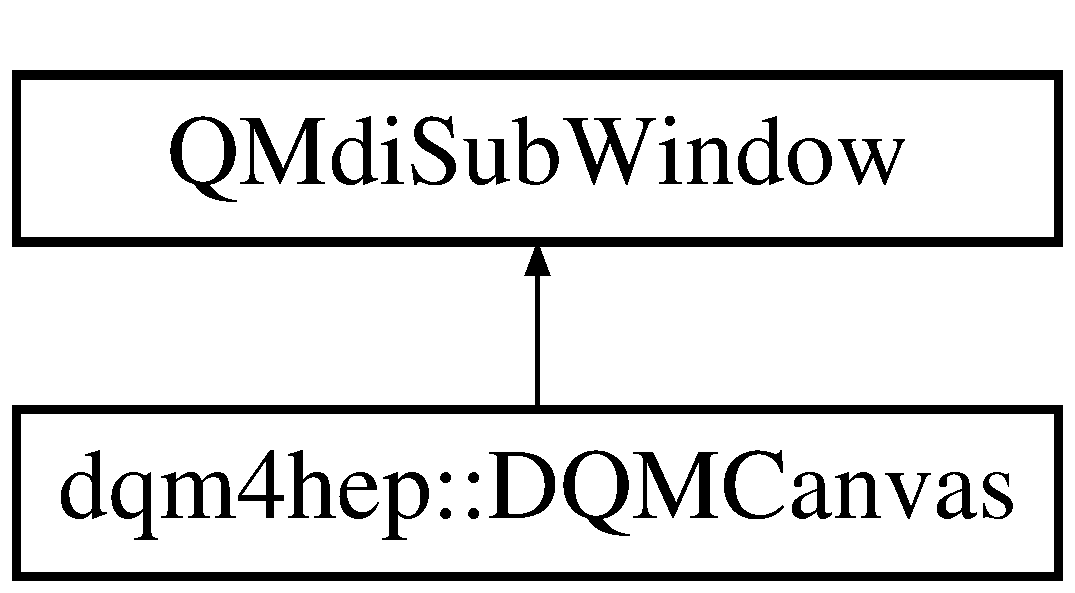
\includegraphics[height=2.000000cm]{classdqm4hep_1_1DQMCanvas}
\end{center}
\end{figure}
\subsection*{Public Slots}
\begin{DoxyCompactItemize}
\item 
void {\bf draw} ({\bf D\+Q\+M\+Gui\+Monitor\+Element} $\ast$p\+Monitor\+Element)
\begin{DoxyCompactList}\small\item\em Draw the monitor element on the root widget. \end{DoxyCompactList}\end{DoxyCompactItemize}
\subsection*{Public Member Functions}
\begin{DoxyCompactItemize}
\item 
{\bf D\+Q\+M\+Canvas} ({\bf D\+Q\+M\+Monitoring} $\ast$p\+Monitoring)
\begin{DoxyCompactList}\small\item\em Constructor. \end{DoxyCompactList}\item 
virtual {\bf $\sim$\+D\+Q\+M\+Canvas} ()
\begin{DoxyCompactList}\small\item\em Destructor. \end{DoxyCompactList}\item 
{\bf D\+Q\+M\+Monitoring} $\ast$ {\bf get\+Monitoring} () const 
\begin{DoxyCompactList}\small\item\em Get the monitoring instance. \end{DoxyCompactList}\item 
{\bf D\+Q\+M\+Gui\+Monitor\+Element} $\ast$ {\bf get\+Current\+Monitor\+Element} () const 
\begin{DoxyCompactList}\small\item\em Get the monitor element currently drawn. \end{DoxyCompactList}\item 
{\bf D\+Q\+M\+Root\+Widget} $\ast$ {\bf get\+Root\+Widget} () const 
\begin{DoxyCompactList}\small\item\em Get the embedded root widget. \end{DoxyCompactList}\end{DoxyCompactItemize}
\subsection*{Protected Attributes}
\begin{DoxyCompactItemize}
\item 
{\bf D\+Q\+M\+Monitoring} $\ast$ {\bf m\+\_\+p\+Monitoring}
\item 
{\bf D\+Q\+M\+Root\+Widget} $\ast$ {\bf m\+\_\+p\+Root\+Widget}
\end{DoxyCompactItemize}


\subsection{Detailed Description}
\doxyref{D\+Q\+M\+Canvas}{p.}{classdqm4hep_1_1DQMCanvas} class. 

Definition at line 46 of file D\+Q\+M\+Canvas.\+h.



\subsection{Constructor \& Destructor Documentation}
\index{dqm4hep\+::\+D\+Q\+M\+Canvas@{dqm4hep\+::\+D\+Q\+M\+Canvas}!D\+Q\+M\+Canvas@{D\+Q\+M\+Canvas}}
\index{D\+Q\+M\+Canvas@{D\+Q\+M\+Canvas}!dqm4hep\+::\+D\+Q\+M\+Canvas@{dqm4hep\+::\+D\+Q\+M\+Canvas}}
\subsubsection[{D\+Q\+M\+Canvas}]{\setlength{\rightskip}{0pt plus 5cm}dqm4hep\+::\+D\+Q\+M\+Canvas\+::\+D\+Q\+M\+Canvas (
\begin{DoxyParamCaption}
\item[{{\bf D\+Q\+M\+Monitoring} $\ast$}]{p\+Monitoring}
\end{DoxyParamCaption}
)}\label{classdqm4hep_1_1DQMCanvas_ac19a5d5b36a897717d04344f06ea24cb}


Constructor. 



Definition at line 36 of file D\+Q\+M\+Canvas.\+cc.



References get\+Monitoring(), m\+\_\+p\+Root\+Widget, and dqm4hep\+::\+D\+Q\+M\+Root\+Widget\+::set\+Canvas().


\begin{DoxyCode}
36                                                :
37     m_pMonitoring(pMonitoring)
38 \{
39   m_pRootWidget = \textcolor{keyword}{new} DQMRootWidget(this->getMonitoring());
40   m_pRootWidget->setCanvas(\textcolor{keyword}{this});
41 
42   setWidget(m_pRootWidget);
43 
44   resize(400, 250);
45 \}
\end{DoxyCode}
\index{dqm4hep\+::\+D\+Q\+M\+Canvas@{dqm4hep\+::\+D\+Q\+M\+Canvas}!````~D\+Q\+M\+Canvas@{$\sim$\+D\+Q\+M\+Canvas}}
\index{````~D\+Q\+M\+Canvas@{$\sim$\+D\+Q\+M\+Canvas}!dqm4hep\+::\+D\+Q\+M\+Canvas@{dqm4hep\+::\+D\+Q\+M\+Canvas}}
\subsubsection[{$\sim$\+D\+Q\+M\+Canvas}]{\setlength{\rightskip}{0pt plus 5cm}dqm4hep\+::\+D\+Q\+M\+Canvas\+::$\sim$\+D\+Q\+M\+Canvas (
\begin{DoxyParamCaption}
{}
\end{DoxyParamCaption}
)\hspace{0.3cm}{\ttfamily [virtual]}}\label{classdqm4hep_1_1DQMCanvas_a7e55d1ca54821f015ea5ab1b0bb7ca21}


Destructor. 



Definition at line 49 of file D\+Q\+M\+Canvas.\+cc.


\begin{DoxyCode}
50 \{
51   \textcolor{comment}{/* nop */}
52 \}
\end{DoxyCode}


\subsection{Member Function Documentation}
\index{dqm4hep\+::\+D\+Q\+M\+Canvas@{dqm4hep\+::\+D\+Q\+M\+Canvas}!draw@{draw}}
\index{draw@{draw}!dqm4hep\+::\+D\+Q\+M\+Canvas@{dqm4hep\+::\+D\+Q\+M\+Canvas}}
\subsubsection[{draw}]{\setlength{\rightskip}{0pt plus 5cm}void dqm4hep\+::\+D\+Q\+M\+Canvas\+::draw (
\begin{DoxyParamCaption}
\item[{{\bf D\+Q\+M\+Gui\+Monitor\+Element} $\ast$}]{p\+Monitor\+Element}
\end{DoxyParamCaption}
)\hspace{0.3cm}{\ttfamily [slot]}}\label{classdqm4hep_1_1DQMCanvas_a062ba344e8e88cb03850b96f287da06d}


Draw the monitor element on the root widget. 



Definition at line 77 of file D\+Q\+M\+Canvas.\+cc.



References dqm4hep\+::\+D\+Q\+M\+Root\+Widget\+::draw(), and m\+\_\+p\+Root\+Widget.



Referenced by dqm4hep\+::\+D\+Q\+M\+Canvas\+Area\+::create\+Canvas(), and dqm4hep\+::\+D\+Q\+M\+Canvas\+Area\+::draw().


\begin{DoxyCode}
78 \{
79   m_pRootWidget->draw(pMonitorElement);
80 \}
\end{DoxyCode}
\index{dqm4hep\+::\+D\+Q\+M\+Canvas@{dqm4hep\+::\+D\+Q\+M\+Canvas}!get\+Current\+Monitor\+Element@{get\+Current\+Monitor\+Element}}
\index{get\+Current\+Monitor\+Element@{get\+Current\+Monitor\+Element}!dqm4hep\+::\+D\+Q\+M\+Canvas@{dqm4hep\+::\+D\+Q\+M\+Canvas}}
\subsubsection[{get\+Current\+Monitor\+Element}]{\setlength{\rightskip}{0pt plus 5cm}{\bf D\+Q\+M\+Gui\+Monitor\+Element} $\ast$ dqm4hep\+::\+D\+Q\+M\+Canvas\+::get\+Current\+Monitor\+Element (
\begin{DoxyParamCaption}
{}
\end{DoxyParamCaption}
) const}\label{classdqm4hep_1_1DQMCanvas_ac32261666c125ffecfea5afbb972e15c}


Get the monitor element currently drawn. 



Definition at line 63 of file D\+Q\+M\+Canvas.\+cc.



References dqm4hep\+::\+D\+Q\+M\+Root\+Widget\+::get\+Current\+Monitor\+Element(), and m\+\_\+p\+Root\+Widget.



Referenced by dqm4hep\+::\+D\+Q\+M\+Canvas\+Area\+::get\+Canvas(), dqm4hep\+::\+D\+Q\+M\+Monitoring\+Controller\+::save\+As(), and dqm4hep\+::\+D\+Q\+M\+Canvas\+View\+::to\+Xml().


\begin{DoxyCode}
64 \{
65   \textcolor{keywordflow}{return} m_pRootWidget->getCurrentMonitorElement();
66 \}
\end{DoxyCode}
\index{dqm4hep\+::\+D\+Q\+M\+Canvas@{dqm4hep\+::\+D\+Q\+M\+Canvas}!get\+Monitoring@{get\+Monitoring}}
\index{get\+Monitoring@{get\+Monitoring}!dqm4hep\+::\+D\+Q\+M\+Canvas@{dqm4hep\+::\+D\+Q\+M\+Canvas}}
\subsubsection[{get\+Monitoring}]{\setlength{\rightskip}{0pt plus 5cm}{\bf D\+Q\+M\+Monitoring} $\ast$ dqm4hep\+::\+D\+Q\+M\+Canvas\+::get\+Monitoring (
\begin{DoxyParamCaption}
{}
\end{DoxyParamCaption}
) const}\label{classdqm4hep_1_1DQMCanvas_a5f36da20fc6efa8534537105e00a2435}


Get the monitoring instance. 



Definition at line 56 of file D\+Q\+M\+Canvas.\+cc.



References m\+\_\+p\+Monitoring.



Referenced by D\+Q\+M\+Canvas(), and dqm4hep\+::\+D\+Q\+M\+Root\+Widget\+::update\+Monitor\+Element().


\begin{DoxyCode}
57 \{
58   \textcolor{keywordflow}{return} m_pMonitoring;
59 \}
\end{DoxyCode}
\index{dqm4hep\+::\+D\+Q\+M\+Canvas@{dqm4hep\+::\+D\+Q\+M\+Canvas}!get\+Root\+Widget@{get\+Root\+Widget}}
\index{get\+Root\+Widget@{get\+Root\+Widget}!dqm4hep\+::\+D\+Q\+M\+Canvas@{dqm4hep\+::\+D\+Q\+M\+Canvas}}
\subsubsection[{get\+Root\+Widget}]{\setlength{\rightskip}{0pt plus 5cm}{\bf D\+Q\+M\+Root\+Widget} $\ast$ dqm4hep\+::\+D\+Q\+M\+Canvas\+::get\+Root\+Widget (
\begin{DoxyParamCaption}
{}
\end{DoxyParamCaption}
) const}\label{classdqm4hep_1_1DQMCanvas_a15616d4e28a33c0519bac3dfbc1957c4}


Get the embedded root widget. 



Definition at line 70 of file D\+Q\+M\+Canvas.\+cc.



References m\+\_\+p\+Root\+Widget.



Referenced by dqm4hep\+::\+D\+Q\+M\+Monitoring\+Controller\+::save\+As().


\begin{DoxyCode}
71 \{
72   \textcolor{keywordflow}{return} m_pRootWidget;
73 \}
\end{DoxyCode}


\subsection{Member Data Documentation}
\index{dqm4hep\+::\+D\+Q\+M\+Canvas@{dqm4hep\+::\+D\+Q\+M\+Canvas}!m\+\_\+p\+Monitoring@{m\+\_\+p\+Monitoring}}
\index{m\+\_\+p\+Monitoring@{m\+\_\+p\+Monitoring}!dqm4hep\+::\+D\+Q\+M\+Canvas@{dqm4hep\+::\+D\+Q\+M\+Canvas}}
\subsubsection[{m\+\_\+p\+Monitoring}]{\setlength{\rightskip}{0pt plus 5cm}{\bf D\+Q\+M\+Monitoring}$\ast$ dqm4hep\+::\+D\+Q\+M\+Canvas\+::m\+\_\+p\+Monitoring\hspace{0.3cm}{\ttfamily [protected]}}\label{classdqm4hep_1_1DQMCanvas_a07d8a9c5b01ada3e3d09051a715f4edc}


Definition at line 78 of file D\+Q\+M\+Canvas.\+h.



Referenced by get\+Monitoring().

\index{dqm4hep\+::\+D\+Q\+M\+Canvas@{dqm4hep\+::\+D\+Q\+M\+Canvas}!m\+\_\+p\+Root\+Widget@{m\+\_\+p\+Root\+Widget}}
\index{m\+\_\+p\+Root\+Widget@{m\+\_\+p\+Root\+Widget}!dqm4hep\+::\+D\+Q\+M\+Canvas@{dqm4hep\+::\+D\+Q\+M\+Canvas}}
\subsubsection[{m\+\_\+p\+Root\+Widget}]{\setlength{\rightskip}{0pt plus 5cm}{\bf D\+Q\+M\+Root\+Widget}$\ast$ dqm4hep\+::\+D\+Q\+M\+Canvas\+::m\+\_\+p\+Root\+Widget\hspace{0.3cm}{\ttfamily [protected]}}\label{classdqm4hep_1_1DQMCanvas_aa7604413c7830ec687edaafbb5b91d16}


Definition at line 79 of file D\+Q\+M\+Canvas.\+h.



Referenced by D\+Q\+M\+Canvas(), draw(), get\+Current\+Monitor\+Element(), and get\+Root\+Widget().



The documentation for this class was generated from the following files\+:\begin{DoxyCompactItemize}
\item 
{\bf D\+Q\+M\+Canvas.\+h}\item 
{\bf D\+Q\+M\+Canvas.\+cc}\end{DoxyCompactItemize}

\section{dqm4hep\+:\+:D\+Q\+M\+Canvas\+Area Class Reference}
\label{classdqm4hep_1_1DQMCanvasArea}\index{dqm4hep\+::\+D\+Q\+M\+Canvas\+Area@{dqm4hep\+::\+D\+Q\+M\+Canvas\+Area}}


\doxyref{D\+Q\+M\+Canvas\+Area}{p.}{classdqm4hep_1_1DQMCanvasArea} class.  




{\ttfamily \#include $<$D\+Q\+M\+Canvas\+Area.\+h$>$}

Inheritance diagram for dqm4hep\+:\+:D\+Q\+M\+Canvas\+Area\+:\begin{figure}[H]
\begin{center}
\leavevmode
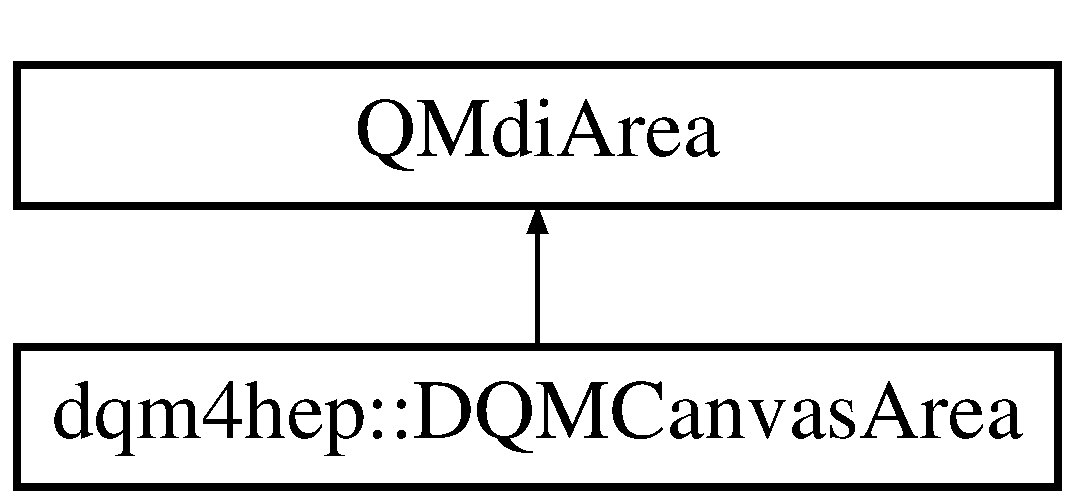
\includegraphics[height=2.000000cm]{classdqm4hep_1_1DQMCanvasArea}
\end{center}
\end{figure}
\subsection*{Public Slots}
\begin{DoxyCompactItemize}
\item 
{\bf D\+Q\+M\+Canvas} $\ast$ {\bf draw} ({\bf D\+Q\+M\+Gui\+Monitor\+Element} $\ast$p\+Monitor\+Element)
\begin{DoxyCompactList}\small\item\em Draw the monitor element. \end{DoxyCompactList}\item 
void {\bf clear} ()
\begin{DoxyCompactList}\small\item\em Clear the canvas area. \end{DoxyCompactList}\end{DoxyCompactItemize}
\subsection*{Public Member Functions}
\begin{DoxyCompactItemize}
\item 
{\bf D\+Q\+M\+Canvas\+Area} ({\bf D\+Q\+M\+Monitoring} $\ast$p\+Monitoring)
\begin{DoxyCompactList}\small\item\em Constructor. \end{DoxyCompactList}\item 
virtual {\bf $\sim$\+D\+Q\+M\+Canvas\+Area} ()
\begin{DoxyCompactList}\small\item\em Destructor. \end{DoxyCompactList}\item 
{\bf D\+Q\+M\+Monitoring} $\ast$ {\bf get\+Monitoring} () const 
\begin{DoxyCompactList}\small\item\em Get the monitoring instance. \end{DoxyCompactList}\item 
bool {\bf is\+Drawn} ({\bf D\+Q\+M\+Gui\+Monitor\+Element} $\ast$p\+Monitor\+Element) const 
\begin{DoxyCompactList}\small\item\em Whether the monitor elemnt is drawn. \end{DoxyCompactList}\item 
bool {\bf remove\+Canvas} ({\bf D\+Q\+M\+Canvas} $\ast$p\+Canvas, bool delete\+Later=false)
\begin{DoxyCompactList}\small\item\em Remove a canvas from the area. \end{DoxyCompactList}\item 
void {\bf add\+Canvas} ({\bf D\+Q\+M\+Canvas} $\ast$p\+Canvas)
\begin{DoxyCompactList}\small\item\em Add a canvas on the area. \end{DoxyCompactList}\item 
int {\bf canvas\+Count} () const 
\begin{DoxyCompactList}\small\item\em Get the number of drawn canvases. \end{DoxyCompactList}\item 
{\bf D\+Q\+M\+Canvas} $\ast$ {\bf create\+Canvas} ({\bf D\+Q\+M\+Gui\+Monitor\+Element} $\ast$p\+Monitor\+Element)
\begin{DoxyCompactList}\small\item\em Create a canvas, add it to the area, draw the monitor element on the root canvas and return it back. \end{DoxyCompactList}\item 
{\bf D\+Q\+M\+Canvas} $\ast$ {\bf get\+Canvas} ({\bf D\+Q\+M\+Gui\+Monitor\+Element} $\ast$p\+Monitor\+Element) const 
\begin{DoxyCompactList}\small\item\em Get the canvas on which the monitor element is drawn. \end{DoxyCompactList}\item 
{\bf D\+Q\+M\+Canvas} $\ast$ {\bf get\+Canvas} (int index) const 
\begin{DoxyCompactList}\small\item\em Get canvas at given index. \end{DoxyCompactList}\item 
bool {\bf contains} ({\bf D\+Q\+M\+Canvas} $\ast$p\+Canvas) const 
\begin{DoxyCompactList}\small\item\em Whether the area contains the given canvas. \end{DoxyCompactList}\end{DoxyCompactItemize}
\subsection*{Protected Attributes}
\begin{DoxyCompactItemize}
\item 
{\bf D\+Q\+M\+Monitoring} $\ast$ {\bf m\+\_\+p\+Monitoring}
\end{DoxyCompactItemize}
\subsection*{Private Member Functions}
\begin{DoxyCompactItemize}
\item 
void {\bf drag\+Enter\+Event} (Q\+Drag\+Enter\+Event $\ast$event)
\item 
void {\bf drop\+Event} (Q\+Drop\+Event $\ast$event)
\end{DoxyCompactItemize}


\subsection{Detailed Description}
\doxyref{D\+Q\+M\+Canvas\+Area}{p.}{classdqm4hep_1_1DQMCanvasArea} class. 

Definition at line 43 of file D\+Q\+M\+Canvas\+Area.\+h.



\subsection{Constructor \& Destructor Documentation}
\index{dqm4hep\+::\+D\+Q\+M\+Canvas\+Area@{dqm4hep\+::\+D\+Q\+M\+Canvas\+Area}!D\+Q\+M\+Canvas\+Area@{D\+Q\+M\+Canvas\+Area}}
\index{D\+Q\+M\+Canvas\+Area@{D\+Q\+M\+Canvas\+Area}!dqm4hep\+::\+D\+Q\+M\+Canvas\+Area@{dqm4hep\+::\+D\+Q\+M\+Canvas\+Area}}
\subsubsection[{D\+Q\+M\+Canvas\+Area}]{\setlength{\rightskip}{0pt plus 5cm}dqm4hep\+::\+D\+Q\+M\+Canvas\+Area\+::\+D\+Q\+M\+Canvas\+Area (
\begin{DoxyParamCaption}
\item[{{\bf D\+Q\+M\+Monitoring} $\ast$}]{p\+Monitoring}
\end{DoxyParamCaption}
)}\label{classdqm4hep_1_1DQMCanvasArea_afd8b6cd9d925b472bb8af680d0084014}


Constructor. 



Definition at line 39 of file D\+Q\+M\+Canvas\+Area.\+cc.


\begin{DoxyCode}
39                                                        :
40     m_pMonitoring(pMonitoring)
41 \{
42   setVerticalScrollBarPolicy(Qt::ScrollBarAsNeeded);
43   setAcceptDrops(\textcolor{keyword}{true});
44 \}
\end{DoxyCode}
\index{dqm4hep\+::\+D\+Q\+M\+Canvas\+Area@{dqm4hep\+::\+D\+Q\+M\+Canvas\+Area}!````~D\+Q\+M\+Canvas\+Area@{$\sim$\+D\+Q\+M\+Canvas\+Area}}
\index{````~D\+Q\+M\+Canvas\+Area@{$\sim$\+D\+Q\+M\+Canvas\+Area}!dqm4hep\+::\+D\+Q\+M\+Canvas\+Area@{dqm4hep\+::\+D\+Q\+M\+Canvas\+Area}}
\subsubsection[{$\sim$\+D\+Q\+M\+Canvas\+Area}]{\setlength{\rightskip}{0pt plus 5cm}dqm4hep\+::\+D\+Q\+M\+Canvas\+Area\+::$\sim$\+D\+Q\+M\+Canvas\+Area (
\begin{DoxyParamCaption}
{}
\end{DoxyParamCaption}
)\hspace{0.3cm}{\ttfamily [virtual]}}\label{classdqm4hep_1_1DQMCanvasArea_ae3c81deabc6f9a0fced2ae5092ad5153}


Destructor. 



Definition at line 48 of file D\+Q\+M\+Canvas\+Area.\+cc.


\begin{DoxyCode}
49 \{
50   \textcolor{comment}{/* nop */}
51 \}
\end{DoxyCode}


\subsection{Member Function Documentation}
\index{dqm4hep\+::\+D\+Q\+M\+Canvas\+Area@{dqm4hep\+::\+D\+Q\+M\+Canvas\+Area}!add\+Canvas@{add\+Canvas}}
\index{add\+Canvas@{add\+Canvas}!dqm4hep\+::\+D\+Q\+M\+Canvas\+Area@{dqm4hep\+::\+D\+Q\+M\+Canvas\+Area}}
\subsubsection[{add\+Canvas}]{\setlength{\rightskip}{0pt plus 5cm}void dqm4hep\+::\+D\+Q\+M\+Canvas\+Area\+::add\+Canvas (
\begin{DoxyParamCaption}
\item[{{\bf D\+Q\+M\+Canvas} $\ast$}]{p\+Canvas}
\end{DoxyParamCaption}
)}\label{classdqm4hep_1_1DQMCanvasArea_a956583ffb4d57336b74f1ffc064c6393}


Add a canvas on the area. 

No action performed if the canvas is already own by the area 

Definition at line 94 of file D\+Q\+M\+Canvas\+Area.\+cc.



Referenced by create\+Canvas(), draw(), and dqm4hep\+::\+D\+Q\+M\+Canvas\+View\+::move\+Canvas().


\begin{DoxyCode}
95 \{
96   \textcolor{keywordflow}{if}(NULL == pCanvasToAdd)
97     \textcolor{keywordflow}{return};
98 
99   QList<QMdiSubWindow*> subWindowList = this->subWindowList();
100 
101   \textcolor{keywordflow}{if}(!subWindowList.contains(pCanvasToAdd))
102     this->addSubWindow(pCanvasToAdd);
103 \}
\end{DoxyCode}
\index{dqm4hep\+::\+D\+Q\+M\+Canvas\+Area@{dqm4hep\+::\+D\+Q\+M\+Canvas\+Area}!canvas\+Count@{canvas\+Count}}
\index{canvas\+Count@{canvas\+Count}!dqm4hep\+::\+D\+Q\+M\+Canvas\+Area@{dqm4hep\+::\+D\+Q\+M\+Canvas\+Area}}
\subsubsection[{canvas\+Count}]{\setlength{\rightskip}{0pt plus 5cm}int dqm4hep\+::\+D\+Q\+M\+Canvas\+Area\+::canvas\+Count (
\begin{DoxyParamCaption}
{}
\end{DoxyParamCaption}
) const}\label{classdqm4hep_1_1DQMCanvasArea_a0d197847e79eb45b3775a4bcc631c32e}


Get the number of drawn canvases. 



Definition at line 191 of file D\+Q\+M\+Canvas\+Area.\+cc.



Referenced by dqm4hep\+::\+D\+Q\+M\+Canvas\+View\+::to\+Xml().


\begin{DoxyCode}
192 \{
193   \textcolor{keywordflow}{return} subWindowList().count();
194 \}
\end{DoxyCode}
\index{dqm4hep\+::\+D\+Q\+M\+Canvas\+Area@{dqm4hep\+::\+D\+Q\+M\+Canvas\+Area}!clear@{clear}}
\index{clear@{clear}!dqm4hep\+::\+D\+Q\+M\+Canvas\+Area@{dqm4hep\+::\+D\+Q\+M\+Canvas\+Area}}
\subsubsection[{clear}]{\setlength{\rightskip}{0pt plus 5cm}void dqm4hep\+::\+D\+Q\+M\+Canvas\+Area\+::clear (
\begin{DoxyParamCaption}
{}
\end{DoxyParamCaption}
)\hspace{0.3cm}{\ttfamily [slot]}}\label{classdqm4hep_1_1DQMCanvasArea_a65999605768c0bee9d1a226ba758a426}


Clear the canvas area. 



Definition at line 242 of file D\+Q\+M\+Canvas\+Area.\+cc.



Referenced by dqm4hep\+::\+D\+Q\+M\+Canvas\+View\+::clear\+Area().


\begin{DoxyCode}
243 \{
244   QList<QMdiSubWindow*>  subWindowList = this->subWindowList();
245 
246   \textcolor{keywordflow}{for}(\textcolor{keywordtype}{int} i=0 ; i<subWindowList.count() ; i++)
247   \{
248     QMdiSubWindow *pSubWindow = subWindowList.at(i);
249 
250     this->removeSubWindow(pSubWindow);
251     pSubWindow->deleteLater();
252   \}
253 \}
\end{DoxyCode}
\index{dqm4hep\+::\+D\+Q\+M\+Canvas\+Area@{dqm4hep\+::\+D\+Q\+M\+Canvas\+Area}!contains@{contains}}
\index{contains@{contains}!dqm4hep\+::\+D\+Q\+M\+Canvas\+Area@{dqm4hep\+::\+D\+Q\+M\+Canvas\+Area}}
\subsubsection[{contains}]{\setlength{\rightskip}{0pt plus 5cm}bool dqm4hep\+::\+D\+Q\+M\+Canvas\+Area\+::contains (
\begin{DoxyParamCaption}
\item[{{\bf D\+Q\+M\+Canvas} $\ast$}]{p\+Canvas}
\end{DoxyParamCaption}
) const}\label{classdqm4hep_1_1DQMCanvasArea_a0c35fccffb1999b08967bcd72eed2a6e}


Whether the area contains the given canvas. 



Definition at line 168 of file D\+Q\+M\+Canvas\+Area.\+cc.



Referenced by dqm4hep\+::\+D\+Q\+M\+Canvas\+View\+::move\+Canvas().


\begin{DoxyCode}
169 \{
170   \textcolor{keywordflow}{if}(!pCanvas)
171     \textcolor{keywordflow}{return} \textcolor{keyword}{false};
172 
173   QList<QMdiSubWindow*>  subWindowList = this->subWindowList();
174 
175   \textcolor{keywordflow}{for}(\textcolor{keywordtype}{int} i=0 ; subWindowList.count() ; i++)
176   \{
177     DQMCanvas *pSubWindow = (DQMCanvas*) subWindowList.at(i);
178 
179     \textcolor{keywordflow}{if}(!pSubWindow)
180       \textcolor{keywordflow}{continue};
181 
182     \textcolor{keywordflow}{if}(pSubWindow == pCanvas)
183       \textcolor{keywordflow}{return} \textcolor{keyword}{true};
184   \}
185 
186   \textcolor{keywordflow}{return} \textcolor{keyword}{false};
187 \}
\end{DoxyCode}
\index{dqm4hep\+::\+D\+Q\+M\+Canvas\+Area@{dqm4hep\+::\+D\+Q\+M\+Canvas\+Area}!create\+Canvas@{create\+Canvas}}
\index{create\+Canvas@{create\+Canvas}!dqm4hep\+::\+D\+Q\+M\+Canvas\+Area@{dqm4hep\+::\+D\+Q\+M\+Canvas\+Area}}
\subsubsection[{create\+Canvas}]{\setlength{\rightskip}{0pt plus 5cm}{\bf D\+Q\+M\+Canvas} $\ast$ dqm4hep\+::\+D\+Q\+M\+Canvas\+Area\+::create\+Canvas (
\begin{DoxyParamCaption}
\item[{{\bf D\+Q\+M\+Gui\+Monitor\+Element} $\ast$}]{p\+Monitor\+Element}
\end{DoxyParamCaption}
)}\label{classdqm4hep_1_1DQMCanvasArea_a742a558a2c1235f5ee8574d222f841e0}


Create a canvas, add it to the area, draw the monitor element on the root canvas and return it back. 



Definition at line 138 of file D\+Q\+M\+Canvas\+Area.\+cc.



References add\+Canvas(), dqm4hep\+::\+D\+Q\+M\+Canvas\+::draw(), get\+Canvas(), and get\+Monitoring().



Referenced by dqm4hep\+::\+D\+Q\+M\+Canvas\+View\+::from\+Xml().


\begin{DoxyCode}
139 \{
140   \textcolor{comment}{// find if this monitor element is drawn an a canvas}
141   DQMCanvas *pCanvas = this->getCanvas(pMonitorElement);
142 
143   \textcolor{keywordflow}{if}(!pCanvas)
144   \{
145     pCanvas = \textcolor{keyword}{new} DQMCanvas(this->getMonitoring());
146     pCanvas->setAttribute(Qt::WA\_DeleteOnClose);
147     this->addCanvas(pCanvas);
148     pCanvas->show();
149   \}
150 
151   pCanvas->show();
152 
153   \textcolor{comment}{// draw it}
154   pCanvas->draw(pMonitorElement);
155 
156   \textcolor{keywordflow}{return} pCanvas;
157 \}
\end{DoxyCode}
\index{dqm4hep\+::\+D\+Q\+M\+Canvas\+Area@{dqm4hep\+::\+D\+Q\+M\+Canvas\+Area}!drag\+Enter\+Event@{drag\+Enter\+Event}}
\index{drag\+Enter\+Event@{drag\+Enter\+Event}!dqm4hep\+::\+D\+Q\+M\+Canvas\+Area@{dqm4hep\+::\+D\+Q\+M\+Canvas\+Area}}
\subsubsection[{drag\+Enter\+Event}]{\setlength{\rightskip}{0pt plus 5cm}void dqm4hep\+::\+D\+Q\+M\+Canvas\+Area\+::drag\+Enter\+Event (
\begin{DoxyParamCaption}
\item[{Q\+Drag\+Enter\+Event $\ast$}]{event}
\end{DoxyParamCaption}
)\hspace{0.3cm}{\ttfamily [private]}}\label{classdqm4hep_1_1DQMCanvasArea_ab7f7296d096244ace327de0f730f5392}


Definition at line 257 of file D\+Q\+M\+Canvas\+Area.\+cc.


\begin{DoxyCode}
258 \{
259   \textcolor{comment}{// check mime type}
260     \textcolor{keywordflow}{if} (pEvent->mimeData()->hasFormat(\textcolor{stringliteral}{"dqm4hep/me-item-list"}))
261       pEvent->acceptProposedAction();
262 \}
\end{DoxyCode}
\index{dqm4hep\+::\+D\+Q\+M\+Canvas\+Area@{dqm4hep\+::\+D\+Q\+M\+Canvas\+Area}!draw@{draw}}
\index{draw@{draw}!dqm4hep\+::\+D\+Q\+M\+Canvas\+Area@{dqm4hep\+::\+D\+Q\+M\+Canvas\+Area}}
\subsubsection[{draw}]{\setlength{\rightskip}{0pt plus 5cm}{\bf D\+Q\+M\+Canvas} $\ast$ dqm4hep\+::\+D\+Q\+M\+Canvas\+Area\+::draw (
\begin{DoxyParamCaption}
\item[{{\bf D\+Q\+M\+Gui\+Monitor\+Element} $\ast$}]{p\+Monitor\+Element}
\end{DoxyParamCaption}
)\hspace{0.3cm}{\ttfamily [slot]}}\label{classdqm4hep_1_1DQMCanvasArea_ab0209e56bf3353506a78e198815f9e1b}


Draw the monitor element. 

Create a new canvas if not already drawn. Return the canvas on which the element is drawn 

Definition at line 198 of file D\+Q\+M\+Canvas\+Area.\+cc.



References add\+Canvas(), dqm4hep\+::\+D\+Q\+M\+Canvas\+::draw(), get\+Canvas(), and get\+Monitoring().



Referenced by dqm4hep\+::\+D\+Q\+M\+Canvas\+View\+::draw\+In\+Area(), dqm4hep\+::\+D\+Q\+M\+Canvas\+View\+::draw\+In\+Current\+Area(), and drop\+Event().


\begin{DoxyCode}
199 \{
200   \textcolor{comment}{// find if this monitor element is drawn an a canvas}
201   DQMCanvas *pCanvas = this->getCanvas(pMonitorElement);
202 
203   DQMCanvas *pCurrentCanvas = qobject\_cast<DQMCanvas *>(this->currentSubWindow());
204   \textcolor{keywordtype}{bool} showMaximized = \textcolor{keyword}{false};
205   \textcolor{keywordtype}{bool} canvasCreated = \textcolor{keyword}{false};
206 
207   \textcolor{keywordflow}{if}(NULL != pCurrentCanvas && pCurrentCanvas->isMaximized())
208     showMaximized = \textcolor{keyword}{true};
209 
210   \textcolor{comment}{// if not, create it}
211   \textcolor{keywordflow}{if}(NULL == pCanvas)
212   \{
213     pCanvas = \textcolor{keyword}{new} DQMCanvas(this->getMonitoring());
214     pCanvas->setAttribute(Qt::WA\_DeleteOnClose);
215     this->addCanvas(pCanvas);
216     canvasCreated = \textcolor{keyword}{true};
217   \}
218 
219   \textcolor{keywordflow}{if}(canvasCreated)
220   \{
221     \textcolor{keywordflow}{if}(showMaximized)
222       pCanvas->showMaximized();
223     \textcolor{keywordflow}{else}
224       pCanvas->show();
225   \}
226   \textcolor{keywordflow}{else}
227   \{
228     \textcolor{keywordflow}{if}(showMaximized)
229       pCanvas->showMaximized();
230     \textcolor{keywordflow}{else}
231       this->setActiveSubWindow(pCanvas);
232   \}
233 
234   \textcolor{comment}{// draw it}
235   pCanvas->draw(pMonitorElement);
236 
237   \textcolor{keywordflow}{return} pCanvas;
238 \}
\end{DoxyCode}
\index{dqm4hep\+::\+D\+Q\+M\+Canvas\+Area@{dqm4hep\+::\+D\+Q\+M\+Canvas\+Area}!drop\+Event@{drop\+Event}}
\index{drop\+Event@{drop\+Event}!dqm4hep\+::\+D\+Q\+M\+Canvas\+Area@{dqm4hep\+::\+D\+Q\+M\+Canvas\+Area}}
\subsubsection[{drop\+Event}]{\setlength{\rightskip}{0pt plus 5cm}void dqm4hep\+::\+D\+Q\+M\+Canvas\+Area\+::drop\+Event (
\begin{DoxyParamCaption}
\item[{Q\+Drop\+Event $\ast$}]{event}
\end{DoxyParamCaption}
)\hspace{0.3cm}{\ttfamily [private]}}\label{classdqm4hep_1_1DQMCanvasArea_a19d213f4b4f4b248ecc7047f56186e7f}


Definition at line 266 of file D\+Q\+M\+Canvas\+Area.\+cc.



References draw(), dqm4hep\+::\+D\+Q\+M\+Monitoring\+Model\+::find\+Monitor\+Element(), dqm4hep\+::\+D\+Q\+M\+Monitoring\+::get\+Controller(), dqm4hep\+::\+D\+Q\+M\+Monitoring\+::get\+Model(), get\+Monitoring(), and dqm4hep\+::\+D\+Q\+M\+Monitoring\+Controller\+::log().


\begin{DoxyCode}
267 \{
268   \textcolor{keywordflow}{if}(pEvent->proposedAction() != Qt::CopyAction)
269     \textcolor{keywordflow}{return};
270 
271   \textcolor{keyword}{const} QByteArray &byteArray(pEvent->mimeData()->data(\textcolor{stringliteral}{"dqm4hep/me-item-list"}));
272 
273   QDataStream dataStream(byteArray);
274 
275   qint32 nElements = 0;
276   dataStream >> nElements;
277 
278   \textcolor{keywordflow}{if}(nElements == 0)
279     \textcolor{keywordflow}{return};
280 
281   \textcolor{comment}{// accept action only if correct type}
282   \textcolor{comment}{// and byte array is not empty}
283   pEvent->acceptProposedAction();
284 
285   \textcolor{keywordtype}{int} nDrawElements = 0;
286 
287   \textcolor{comment}{// deserialize the items, query the element}
288   \textcolor{comment}{// to model and draw them on the fly}
289   \textcolor{keywordflow}{for}(\textcolor{keywordtype}{int} i=0 ; i < nElements ; i++)
290   \{
291     QString collectorName;
292     QString moduleName;
293     QString fullPathName;
294     QString monitorElementName;
295 
296     dataStream >> collectorName >> moduleName >> fullPathName >> monitorElementName;
297 
298     DQMGuiMonitorElement *pMonitorElement =
299         this->getMonitoring()->getModel()->findMonitorElement(
300             collectorName.toStdString(),
301             moduleName.toStdString(),
302             fullPathName.toStdString(),
303             monitorElementName.toStdString());
304 
305     \textcolor{keywordflow}{if}(!pMonitorElement)
306       \textcolor{keywordflow}{continue};
307 
308     this->draw(pMonitorElement);
309     nDrawElements++;
310   \}
311 
312   \textcolor{keywordflow}{if}(nDrawElements == nElements)
313     this->getMonitoring()->getController()->log(MESSAGE, QString(\textcolor{stringliteral}{"Number of drawn monitor elements : %1"}).
      arg(nDrawElements).toStdString());
314   \textcolor{keywordflow}{else} \textcolor{keywordflow}{if}(nDrawElements < nElements && nDrawElements != 0)
315     this->getMonitoring()->getController()->log(WARNING, QString(\textcolor{stringliteral}{"Monitor elements drawn (%1 success, %2
       failed)"}).arg(nDrawElements).arg(nElements-nDrawElements).toStdString());
316   \textcolor{keywordflow}{else}
317     this->getMonitoring()->getController()->log(ERROR, QString(\textcolor{stringliteral}{"No monitor elements drawn ! (%1 requested)"}
      ).arg(nElements).toStdString());
318 \}
\end{DoxyCode}
\index{dqm4hep\+::\+D\+Q\+M\+Canvas\+Area@{dqm4hep\+::\+D\+Q\+M\+Canvas\+Area}!get\+Canvas@{get\+Canvas}}
\index{get\+Canvas@{get\+Canvas}!dqm4hep\+::\+D\+Q\+M\+Canvas\+Area@{dqm4hep\+::\+D\+Q\+M\+Canvas\+Area}}
\subsubsection[{get\+Canvas}]{\setlength{\rightskip}{0pt plus 5cm}{\bf D\+Q\+M\+Canvas} $\ast$ dqm4hep\+::\+D\+Q\+M\+Canvas\+Area\+::get\+Canvas (
\begin{DoxyParamCaption}
\item[{{\bf D\+Q\+M\+Gui\+Monitor\+Element} $\ast$}]{p\+Monitor\+Element}
\end{DoxyParamCaption}
) const}\label{classdqm4hep_1_1DQMCanvasArea_a705d7fe6c5addeb32cc206f69a2e1024}


Get the canvas on which the monitor element is drawn. 



Definition at line 107 of file D\+Q\+M\+Canvas\+Area.\+cc.



References dqm4hep\+::\+D\+Q\+M\+Gui\+Monitor\+Element\+::equals(), and dqm4hep\+::\+D\+Q\+M\+Canvas\+::get\+Current\+Monitor\+Element().



Referenced by create\+Canvas(), draw(), is\+Drawn(), and dqm4hep\+::\+D\+Q\+M\+Canvas\+View\+::to\+Xml().


\begin{DoxyCode}
108 \{
109   \textcolor{keywordflow}{if}(NULL == pMonitorElement)
110     \textcolor{keywordflow}{return} NULL;
111 
112   QList<QMdiSubWindow*>  subWindowList = this->subWindowList();
113 
114   \textcolor{keywordflow}{for}(\textcolor{keywordtype}{int} i=0 ; i<subWindowList.count() ; i++)
115   \{
116     DQMCanvas *pCanvas = (DQMCanvas *) subWindowList.at(i);
117 
118     \textcolor{keywordflow}{if}(!pCanvas)
119       \textcolor{keywordflow}{continue};
120 
121     DQMGuiMonitorElement *pCurrentMonitorElement = pCanvas->getCurrentMonitorElement();
122 
123     \textcolor{keywordflow}{if}(NULL == pCurrentMonitorElement)
124       \textcolor{keywordflow}{continue};
125 
126     \textcolor{keywordflow}{if}(pMonitorElement == pCurrentMonitorElement)
127       \textcolor{keywordflow}{return} pCanvas;
128 
129     \textcolor{keywordflow}{if}(pMonitorElement->equals(pCurrentMonitorElement))
130       \textcolor{keywordflow}{return} pCanvas;
131   \}
132 
133   \textcolor{keywordflow}{return} NULL;
134 \}
\end{DoxyCode}
\index{dqm4hep\+::\+D\+Q\+M\+Canvas\+Area@{dqm4hep\+::\+D\+Q\+M\+Canvas\+Area}!get\+Canvas@{get\+Canvas}}
\index{get\+Canvas@{get\+Canvas}!dqm4hep\+::\+D\+Q\+M\+Canvas\+Area@{dqm4hep\+::\+D\+Q\+M\+Canvas\+Area}}
\subsubsection[{get\+Canvas}]{\setlength{\rightskip}{0pt plus 5cm}{\bf D\+Q\+M\+Canvas} $\ast$ dqm4hep\+::\+D\+Q\+M\+Canvas\+Area\+::get\+Canvas (
\begin{DoxyParamCaption}
\item[{int}]{index}
\end{DoxyParamCaption}
) const}\label{classdqm4hep_1_1DQMCanvasArea_a97e599c3bfaa2048c64a1014f7c3af45}


Get canvas at given index. 



Definition at line 161 of file D\+Q\+M\+Canvas\+Area.\+cc.


\begin{DoxyCode}
162 \{
163   \textcolor{keywordflow}{return} (DQMCanvas *) this->subWindowList().at(index);
164 \}
\end{DoxyCode}
\index{dqm4hep\+::\+D\+Q\+M\+Canvas\+Area@{dqm4hep\+::\+D\+Q\+M\+Canvas\+Area}!get\+Monitoring@{get\+Monitoring}}
\index{get\+Monitoring@{get\+Monitoring}!dqm4hep\+::\+D\+Q\+M\+Canvas\+Area@{dqm4hep\+::\+D\+Q\+M\+Canvas\+Area}}
\subsubsection[{get\+Monitoring}]{\setlength{\rightskip}{0pt plus 5cm}{\bf D\+Q\+M\+Monitoring} $\ast$ dqm4hep\+::\+D\+Q\+M\+Canvas\+Area\+::get\+Monitoring (
\begin{DoxyParamCaption}
{}
\end{DoxyParamCaption}
) const}\label{classdqm4hep_1_1DQMCanvasArea_abde8068d54f7708e40117e065705831b}


Get the monitoring instance. 



Definition at line 55 of file D\+Q\+M\+Canvas\+Area.\+cc.



References m\+\_\+p\+Monitoring.



Referenced by create\+Canvas(), draw(), and drop\+Event().


\begin{DoxyCode}
56 \{
57   \textcolor{keywordflow}{return} m_pMonitoring;
58 \}
\end{DoxyCode}
\index{dqm4hep\+::\+D\+Q\+M\+Canvas\+Area@{dqm4hep\+::\+D\+Q\+M\+Canvas\+Area}!is\+Drawn@{is\+Drawn}}
\index{is\+Drawn@{is\+Drawn}!dqm4hep\+::\+D\+Q\+M\+Canvas\+Area@{dqm4hep\+::\+D\+Q\+M\+Canvas\+Area}}
\subsubsection[{is\+Drawn}]{\setlength{\rightskip}{0pt plus 5cm}bool dqm4hep\+::\+D\+Q\+M\+Canvas\+Area\+::is\+Drawn (
\begin{DoxyParamCaption}
\item[{{\bf D\+Q\+M\+Gui\+Monitor\+Element} $\ast$}]{p\+Monitor\+Element}
\end{DoxyParamCaption}
) const}\label{classdqm4hep_1_1DQMCanvasArea_aa6aa7ee23a9ef51be862568d4a980f46}


Whether the monitor elemnt is drawn. 

Comparison done by ptr or full name (path + name) 

Definition at line 62 of file D\+Q\+M\+Canvas\+Area.\+cc.



References get\+Canvas().


\begin{DoxyCode}
63 \{
64   \textcolor{keywordflow}{return} (NULL == this->getCanvas(pMonitorElement));
65 \}
\end{DoxyCode}
\index{dqm4hep\+::\+D\+Q\+M\+Canvas\+Area@{dqm4hep\+::\+D\+Q\+M\+Canvas\+Area}!remove\+Canvas@{remove\+Canvas}}
\index{remove\+Canvas@{remove\+Canvas}!dqm4hep\+::\+D\+Q\+M\+Canvas\+Area@{dqm4hep\+::\+D\+Q\+M\+Canvas\+Area}}
\subsubsection[{remove\+Canvas}]{\setlength{\rightskip}{0pt plus 5cm}bool dqm4hep\+::\+D\+Q\+M\+Canvas\+Area\+::remove\+Canvas (
\begin{DoxyParamCaption}
\item[{{\bf D\+Q\+M\+Canvas} $\ast$}]{p\+Canvas, }
\item[{bool}]{delete\+Later = {\ttfamily false}}
\end{DoxyParamCaption}
)}\label{classdqm4hep_1_1DQMCanvasArea_aa67dded293e3ea24f685925edeaa4ef8}


Remove a canvas from the area. 

The canvas is not deleted. No action performed if the area does not own the canvas Return whether the canvas has been removed 

Definition at line 69 of file D\+Q\+M\+Canvas\+Area.\+cc.



Referenced by dqm4hep\+::\+D\+Q\+M\+Canvas\+View\+::move\+Canvas(), and dqm4hep\+::\+D\+Q\+M\+Root\+Widget\+::remove\+Canvas().


\begin{DoxyCode}
70 \{
71   \textcolor{keywordflow}{if}(NULL == pCanvasToRemove)
72     \textcolor{keywordflow}{return} \textcolor{keyword}{false};
73 
74   QList<QMdiSubWindow*> subWindowList = this->subWindowList();
75 
76   \textcolor{keywordflow}{for}(\textcolor{keywordtype}{int} i=0 ; subWindowList.count() ; i++)
77   \{
78     \textcolor{keywordflow}{if}(pCanvasToRemove == subWindowList.at(i))
79     \{
80       this->removeSubWindow(pCanvasToRemove);
81 
82       \textcolor{keywordflow}{if}(deleteLater)
83         pCanvasToRemove->deleteLater();
84 
85       \textcolor{keywordflow}{return} \textcolor{keyword}{true};
86     \}
87   \}
88 
89   \textcolor{keywordflow}{return} \textcolor{keyword}{false};
90 \}
\end{DoxyCode}


\subsection{Member Data Documentation}
\index{dqm4hep\+::\+D\+Q\+M\+Canvas\+Area@{dqm4hep\+::\+D\+Q\+M\+Canvas\+Area}!m\+\_\+p\+Monitoring@{m\+\_\+p\+Monitoring}}
\index{m\+\_\+p\+Monitoring@{m\+\_\+p\+Monitoring}!dqm4hep\+::\+D\+Q\+M\+Canvas\+Area@{dqm4hep\+::\+D\+Q\+M\+Canvas\+Area}}
\subsubsection[{m\+\_\+p\+Monitoring}]{\setlength{\rightskip}{0pt plus 5cm}{\bf D\+Q\+M\+Monitoring}$\ast$ dqm4hep\+::\+D\+Q\+M\+Canvas\+Area\+::m\+\_\+p\+Monitoring\hspace{0.3cm}{\ttfamily [protected]}}\label{classdqm4hep_1_1DQMCanvasArea_a44221699421cb7a453b8d9aa4a249de2}


Definition at line 118 of file D\+Q\+M\+Canvas\+Area.\+h.



Referenced by get\+Monitoring().



The documentation for this class was generated from the following files\+:\begin{DoxyCompactItemize}
\item 
{\bf D\+Q\+M\+Canvas\+Area.\+h}\item 
{\bf D\+Q\+M\+Canvas\+Area.\+cc}\end{DoxyCompactItemize}

\section{dqm4hep\+:\+:D\+Q\+M\+Canvas\+View Class Reference}
\label{classdqm4hep_1_1DQMCanvasView}\index{dqm4hep\+::\+D\+Q\+M\+Canvas\+View@{dqm4hep\+::\+D\+Q\+M\+Canvas\+View}}


\doxyref{D\+Q\+M\+Canvas\+View}{p.}{classdqm4hep_1_1DQMCanvasView} class.  




{\ttfamily \#include $<$D\+Q\+M\+Canvas\+View.\+h$>$}

Inheritance diagram for dqm4hep\+:\+:D\+Q\+M\+Canvas\+View\+:\begin{figure}[H]
\begin{center}
\leavevmode
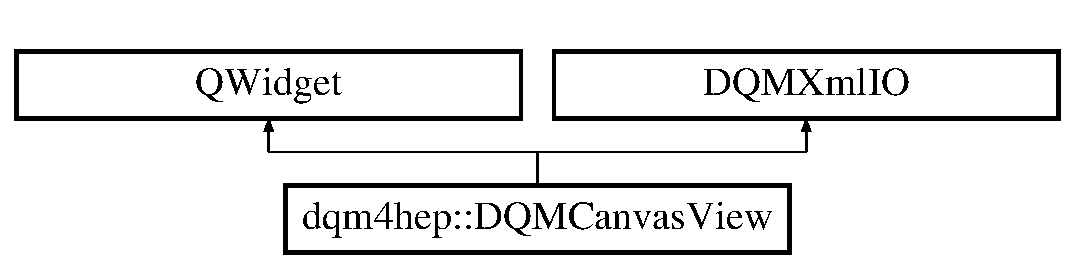
\includegraphics[height=2.000000cm]{classdqm4hep_1_1DQMCanvasView}
\end{center}
\end{figure}
\subsection*{Public Slots}
\begin{DoxyCompactItemize}
\item 
virtual void {\bf create\+Canvas\+Area} (const std\+::string \&area\+Name=\char`\"{}\char`\"{})
\begin{DoxyCompactList}\small\item\em Create a canvas area. \end{DoxyCompactList}\item 
virtual void {\bf create\+Canvas\+Area\+And\+Set\+Current} (const std\+::string \&area\+Name=\char`\"{}\char`\"{})
\begin{DoxyCompactList}\small\item\em Create a canvas area and set it as current. \end{DoxyCompactList}\item 
virtual void {\bf draw\+In\+Current\+Area} ({\bf D\+Q\+M\+Gui\+Monitor\+Element} $\ast$p\+Monitor\+Element)
\begin{DoxyCompactList}\small\item\em Draw the monitor element in the current area. \end{DoxyCompactList}\item 
virtual void {\bf draw\+In\+Area} ({\bf D\+Q\+M\+Gui\+Monitor\+Element} $\ast$p\+Monitor\+Element, int index)
\begin{DoxyCompactList}\small\item\em Draw the monitor element in area indexed by 'index'. \end{DoxyCompactList}\item 
virtual void {\bf draw\+In\+New\+Area} ({\bf D\+Q\+M\+Gui\+Monitor\+Element} $\ast$p\+Monitor\+Element, const std\+::string \&area\+Name=\char`\"{}\char`\"{})
\begin{DoxyCompactList}\small\item\em Draw the monitor element in a new area. \end{DoxyCompactList}\item 
virtual void {\bf remove\+Canvas\+Area} (int index)
\begin{DoxyCompactList}\small\item\em Remove the canvas area by index. \end{DoxyCompactList}\item 
virtual void {\bf rename\+Canvas\+Area} (int index, const std\+::string \&new\+Area\+Name)
\begin{DoxyCompactList}\small\item\em Rename the canvas area indexed by 'index' with name 'new\+Area\+Name'. \end{DoxyCompactList}\item 
virtual void {\bf clear\+Area} (int index)
\begin{DoxyCompactList}\small\item\em Clear the area indexed by 'index'. \end{DoxyCompactList}\item 
virtual void {\bf clear} ()
\begin{DoxyCompactList}\small\item\em Clear and remove all canvas areas. \end{DoxyCompactList}\item 
virtual void {\bf show\+Context\+Menu} (const Q\+Point \&point)
\begin{DoxyCompactList}\small\item\em Show the context menu of this widget. \end{DoxyCompactList}\item 
virtual void {\bf set\+Current\+Canvas\+Area} (int index)
\begin{DoxyCompactList}\small\item\em Set the current canvas area by index. \end{DoxyCompactList}\item 
virtual void {\bf move\+Canvas} ({\bf D\+Q\+M\+Canvas} $\ast$p\+Canvas, int new\+Area\+Index)
\begin{DoxyCompactList}\small\item\em Move the canvas from the current area to the area indexed by 'index'. \end{DoxyCompactList}\end{DoxyCompactItemize}
\subsection*{Public Member Functions}
\begin{DoxyCompactItemize}
\item 
{\bf D\+Q\+M\+Canvas\+View} ({\bf D\+Q\+M\+Monitoring} $\ast$p\+Monitoring, Q\+Widget $\ast$p\+Parent=0)
\begin{DoxyCompactList}\small\item\em Constructor. \end{DoxyCompactList}\item 
virtual {\bf $\sim$\+D\+Q\+M\+Canvas\+View} ()
\begin{DoxyCompactList}\small\item\em Destructor. \end{DoxyCompactList}\item 
{\bf D\+Q\+M\+Monitoring} $\ast$ {\bf get\+Monitoring} () const 
\begin{DoxyCompactList}\small\item\em Get the monitoring instance. \end{DoxyCompactList}\item 
Ti\+Xml\+Element $\ast$ {\bf to\+Xml} () const 
\begin{DoxyCompactList}\small\item\em Export settings to xml element. \end{DoxyCompactList}\item 
void {\bf from\+Xml} (Ti\+Xml\+Element $\ast$const p\+Xml\+Element)
\begin{DoxyCompactList}\small\item\em Import settings from xml element. \end{DoxyCompactList}\item 
virtual {\bf D\+Q\+M\+Canvas\+Area} $\ast$ {\bf get\+Current\+Canvas\+Area} () const 
\begin{DoxyCompactList}\small\item\em Get the current canvas area. \end{DoxyCompactList}\item 
virtual std\+::string {\bf get\+Current\+Canvas\+Area\+Name} () const 
\begin{DoxyCompactList}\small\item\em Get the current canvas area name. \end{DoxyCompactList}\item 
virtual {\bf D\+Q\+M\+Canvas\+Area} $\ast$ {\bf get\+Canvas\+Area} (int index) const 
\begin{DoxyCompactList}\small\item\em Get the canvas area by index. \end{DoxyCompactList}\item 
virtual int {\bf get\+Canvas\+Area\+Index} ({\bf D\+Q\+M\+Canvas\+Area} $\ast$p\+Canvas\+Area) const 
\begin{DoxyCompactList}\small\item\em Get the canvas area index using an instance of canvas area. \end{DoxyCompactList}\item 
virtual std\+::string {\bf get\+Canvas\+Area\+Name} (int index) const 
\begin{DoxyCompactList}\small\item\em Get the canvas area name by index. \end{DoxyCompactList}\item 
virtual int {\bf canvas\+Area\+Count} () const 
\begin{DoxyCompactList}\small\item\em Get the number of canvas areas. \end{DoxyCompactList}\item 
virtual Q\+List$<$ {\bf D\+Q\+M\+Canvas\+Area} $\ast$ $>$ {\bf canvas\+Area\+List} () const 
\begin{DoxyCompactList}\small\item\em Get the canvas area list. \end{DoxyCompactList}\end{DoxyCompactItemize}
\subsection*{Protected Member Functions}
\begin{DoxyCompactItemize}
\item 
virtual bool {\bf event\+Filter} (Q\+Object $\ast$p\+Object, Q\+Event $\ast$p\+Event)
\begin{DoxyCompactList}\small\item\em Event filter mainly used to process the context menu. \end{DoxyCompactList}\item 
virtual Q\+Menu $\ast$ {\bf create\+Context\+Menu} () const 
\begin{DoxyCompactList}\small\item\em Create the context menu. \end{DoxyCompactList}\item 
void {\bf rename\+Canvas\+Area\+From\+Input\+Dialog} (int index)
\begin{DoxyCompactList}\small\item\em Rename the canvas area given by 'index'. \end{DoxyCompactList}\end{DoxyCompactItemize}
\subsection*{Private Slots}
\begin{DoxyCompactItemize}
\item 
void {\bf handle\+Rename\+Area\+Action\+Triggered} ()
\begin{DoxyCompactList}\small\item\em Handle rename area action triggered by context menu. \end{DoxyCompactList}\item 
void {\bf handle\+Remove\+Area\+Action\+Triggered} ()
\begin{DoxyCompactList}\small\item\em Handle remove area action triggered by context menu. \end{DoxyCompactList}\item 
void {\bf handle\+Clear\+Area\+Action\+Triggered} ()
\begin{DoxyCompactList}\small\item\em Handle clear area action triggered by context menu. \end{DoxyCompactList}\item 
void {\bf handle\+Save\+As\+Action\+Triggered} ()
\begin{DoxyCompactList}\small\item\em Handle save as action triggered by context menu. \end{DoxyCompactList}\end{DoxyCompactItemize}
\subsection*{Private Attributes}
\begin{DoxyCompactItemize}
\item 
{\bf D\+Q\+M\+Monitoring} $\ast$ {\bf m\+\_\+p\+Monitoring}
\item 
{\bf D\+Q\+M\+Tab\+Widget} $\ast$ {\bf m\+\_\+p\+Tab\+Widget}
\end{DoxyCompactItemize}


\subsection{Detailed Description}
\doxyref{D\+Q\+M\+Canvas\+View}{p.}{classdqm4hep_1_1DQMCanvasView} class. 

Definition at line 51 of file D\+Q\+M\+Canvas\+View.\+h.



\subsection{Constructor \& Destructor Documentation}
\index{dqm4hep\+::\+D\+Q\+M\+Canvas\+View@{dqm4hep\+::\+D\+Q\+M\+Canvas\+View}!D\+Q\+M\+Canvas\+View@{D\+Q\+M\+Canvas\+View}}
\index{D\+Q\+M\+Canvas\+View@{D\+Q\+M\+Canvas\+View}!dqm4hep\+::\+D\+Q\+M\+Canvas\+View@{dqm4hep\+::\+D\+Q\+M\+Canvas\+View}}
\subsubsection[{D\+Q\+M\+Canvas\+View}]{\setlength{\rightskip}{0pt plus 5cm}dqm4hep\+::\+D\+Q\+M\+Canvas\+View\+::\+D\+Q\+M\+Canvas\+View (
\begin{DoxyParamCaption}
\item[{{\bf D\+Q\+M\+Monitoring} $\ast$}]{p\+Monitoring, }
\item[{Q\+Widget $\ast$}]{p\+Parent = {\ttfamily 0}}
\end{DoxyParamCaption}
)}\label{classdqm4hep_1_1DQMCanvasView_a6b5a2e3be9a867b707ccf9c72f78cd8b}


Constructor. 



Definition at line 84 of file D\+Q\+M\+Canvas\+View.\+cc.



References create\+Canvas\+Area(), m\+\_\+p\+Tab\+Widget, and remove\+Canvas\+Area().


\begin{DoxyCode}
84                                                                          :
85     QWidget(pParent),
86     m_pMonitoring(pMonitoring)
87 \{
88   setLayout(\textcolor{keyword}{new} QHBoxLayout());
89   m_pTabWidget = \textcolor{keyword}{new} DQMTabWidget(\textcolor{keyword}{this});
90   layout()->addWidget(m_pTabWidget);
91   m_pTabWidget->installEventFilter(\textcolor{keyword}{this});
92 
93   m_pTabWidget->setMovable(\textcolor{keyword}{true});
94   m_pTabWidget->setTabsClosable(\textcolor{keyword}{true});
95 
96     QToolButton *pButton = \textcolor{keyword}{new} QToolButton(m_pTabWidget);
97     pButton->setText(\textcolor{stringliteral}{"+"});
98     pButton->setAutoRaise(\textcolor{keyword}{true});
99     m_pTabWidget->setCornerWidget(pButton);
100 
101   this->createCanvasArea(\textcolor{stringliteral}{"Canvas area"});
102 
103   connect(m_pTabWidget, SIGNAL(tabCloseRequested(\textcolor{keywordtype}{int})), \textcolor{keyword}{this}, SLOT(
      removeCanvasArea(\textcolor{keywordtype}{int})));
104   connect(pButton, SIGNAL(clicked()), \textcolor{keyword}{this}, SLOT(createCanvasArea()));
105 
106   installEventFilter(\textcolor{keyword}{this});
107 \}
\end{DoxyCode}
\index{dqm4hep\+::\+D\+Q\+M\+Canvas\+View@{dqm4hep\+::\+D\+Q\+M\+Canvas\+View}!````~D\+Q\+M\+Canvas\+View@{$\sim$\+D\+Q\+M\+Canvas\+View}}
\index{````~D\+Q\+M\+Canvas\+View@{$\sim$\+D\+Q\+M\+Canvas\+View}!dqm4hep\+::\+D\+Q\+M\+Canvas\+View@{dqm4hep\+::\+D\+Q\+M\+Canvas\+View}}
\subsubsection[{$\sim$\+D\+Q\+M\+Canvas\+View}]{\setlength{\rightskip}{0pt plus 5cm}dqm4hep\+::\+D\+Q\+M\+Canvas\+View\+::$\sim$\+D\+Q\+M\+Canvas\+View (
\begin{DoxyParamCaption}
{}
\end{DoxyParamCaption}
)\hspace{0.3cm}{\ttfamily [virtual]}}\label{classdqm4hep_1_1DQMCanvasView_a444206f3e7ae281f8ddff4a2c77f1954}


Destructor. 



Definition at line 111 of file D\+Q\+M\+Canvas\+View.\+cc.



References get\+Canvas\+Area(), and m\+\_\+p\+Tab\+Widget.


\begin{DoxyCode}
112 \{
113   \textcolor{keywordflow}{while}(m_pTabWidget->count() != 0)
114   \{
115     DQMCanvasArea *pCanvasArea = this->getCanvasArea(0);
116     m_pTabWidget->removeTab(0);
117     pCanvasArea->deleteLater();
118   \}
119 \}
\end{DoxyCode}


\subsection{Member Function Documentation}
\index{dqm4hep\+::\+D\+Q\+M\+Canvas\+View@{dqm4hep\+::\+D\+Q\+M\+Canvas\+View}!canvas\+Area\+Count@{canvas\+Area\+Count}}
\index{canvas\+Area\+Count@{canvas\+Area\+Count}!dqm4hep\+::\+D\+Q\+M\+Canvas\+View@{dqm4hep\+::\+D\+Q\+M\+Canvas\+View}}
\subsubsection[{canvas\+Area\+Count}]{\setlength{\rightskip}{0pt plus 5cm}int dqm4hep\+::\+D\+Q\+M\+Canvas\+View\+::canvas\+Area\+Count (
\begin{DoxyParamCaption}
{}
\end{DoxyParamCaption}
) const\hspace{0.3cm}{\ttfamily [virtual]}}\label{classdqm4hep_1_1DQMCanvasView_ad92ac996828263b3c72806295e432875}


Get the number of canvas areas. 



Definition at line 335 of file D\+Q\+M\+Canvas\+View.\+cc.



References m\+\_\+p\+Tab\+Widget.



Referenced by dqm4hep\+::\+D\+Q\+M\+Monitor\+Element\+Navigator\+::draw\+Selected\+Monitor\+Elements(), dqm4hep\+::\+D\+Q\+M\+Monitor\+Element\+Navigator\+::show\+Context\+Menu(), and to\+Xml().


\begin{DoxyCode}
336 \{
337   \textcolor{keywordflow}{return} m_pTabWidget->count();
338 \}
\end{DoxyCode}
\index{dqm4hep\+::\+D\+Q\+M\+Canvas\+View@{dqm4hep\+::\+D\+Q\+M\+Canvas\+View}!canvas\+Area\+List@{canvas\+Area\+List}}
\index{canvas\+Area\+List@{canvas\+Area\+List}!dqm4hep\+::\+D\+Q\+M\+Canvas\+View@{dqm4hep\+::\+D\+Q\+M\+Canvas\+View}}
\subsubsection[{canvas\+Area\+List}]{\setlength{\rightskip}{0pt plus 5cm}Q\+List$<$ {\bf D\+Q\+M\+Canvas\+Area} $\ast$ $>$ dqm4hep\+::\+D\+Q\+M\+Canvas\+View\+::canvas\+Area\+List (
\begin{DoxyParamCaption}
{}
\end{DoxyParamCaption}
) const\hspace{0.3cm}{\ttfamily [virtual]}}\label{classdqm4hep_1_1DQMCanvasView_adfc267abfec3b1c49fb765f85bdea2a4}


Get the canvas area list. 



Definition at line 342 of file D\+Q\+M\+Canvas\+View.\+cc.



References get\+Canvas\+Area(), and m\+\_\+p\+Tab\+Widget.



Referenced by dqm4hep\+::\+D\+Q\+M\+Root\+Widget\+::create\+Context\+Menu().


\begin{DoxyCode}
343 \{
344   QList<DQMCanvasArea*> list;
345 
346   \textcolor{keywordflow}{for}(\textcolor{keywordtype}{int} i=0 ; i<m_pTabWidget->count() ; i++)
347   \{
348     DQMCanvasArea *pCanvasArea = this->getCanvasArea(i);
349 
350     \textcolor{keywordflow}{if}(!pCanvasArea)
351       \textcolor{keywordflow}{continue};
352 
353     list.append(pCanvasArea);
354   \}
355 
356   \textcolor{keywordflow}{return} list;
357 \}
\end{DoxyCode}
\index{dqm4hep\+::\+D\+Q\+M\+Canvas\+View@{dqm4hep\+::\+D\+Q\+M\+Canvas\+View}!clear@{clear}}
\index{clear@{clear}!dqm4hep\+::\+D\+Q\+M\+Canvas\+View@{dqm4hep\+::\+D\+Q\+M\+Canvas\+View}}
\subsubsection[{clear}]{\setlength{\rightskip}{0pt plus 5cm}void dqm4hep\+::\+D\+Q\+M\+Canvas\+View\+::clear (
\begin{DoxyParamCaption}
{}
\end{DoxyParamCaption}
)\hspace{0.3cm}{\ttfamily [virtual]}, {\ttfamily [slot]}}\label{classdqm4hep_1_1DQMCanvasView_ab28aeb52e05d99a3d8708b3d38503051}


Clear and remove all canvas areas. 



Definition at line 445 of file D\+Q\+M\+Canvas\+View.\+cc.



References create\+Canvas\+Area(), get\+Canvas\+Area(), and m\+\_\+p\+Tab\+Widget.



Referenced by dqm4hep\+::\+D\+Q\+M\+Monitoring\+View\+::clear(), and create\+Context\+Menu().


\begin{DoxyCode}
446 \{
447   \textcolor{keywordflow}{while}(m_pTabWidget->count() != 0)
448   \{
449     DQMCanvasArea *pCanvasArea = this->getCanvasArea(0);
450     m_pTabWidget->removeTab(0);
451     pCanvasArea->deleteLater();
452   \}
453 
454   this->createCanvasArea();
455 \}
\end{DoxyCode}
\index{dqm4hep\+::\+D\+Q\+M\+Canvas\+View@{dqm4hep\+::\+D\+Q\+M\+Canvas\+View}!clear\+Area@{clear\+Area}}
\index{clear\+Area@{clear\+Area}!dqm4hep\+::\+D\+Q\+M\+Canvas\+View@{dqm4hep\+::\+D\+Q\+M\+Canvas\+View}}
\subsubsection[{clear\+Area}]{\setlength{\rightskip}{0pt plus 5cm}void dqm4hep\+::\+D\+Q\+M\+Canvas\+View\+::clear\+Area (
\begin{DoxyParamCaption}
\item[{int}]{index}
\end{DoxyParamCaption}
)\hspace{0.3cm}{\ttfamily [virtual]}, {\ttfamily [slot]}}\label{classdqm4hep_1_1DQMCanvasView_ab8f6f6fd381ef3f0a1cfed84ab182c75}


Clear the area indexed by 'index'. 



Definition at line 433 of file D\+Q\+M\+Canvas\+View.\+cc.



References dqm4hep\+::\+D\+Q\+M\+Canvas\+Area\+::clear(), and get\+Canvas\+Area().



Referenced by handle\+Clear\+Area\+Action\+Triggered().


\begin{DoxyCode}
434 \{
435   DQMCanvasArea *pCanvasArea = this->getCanvasArea(index);
436 
437   \textcolor{keywordflow}{if}(!pCanvasArea)
438     \textcolor{keywordflow}{return};
439 
440   pCanvasArea->clear();
441 \}
\end{DoxyCode}
\index{dqm4hep\+::\+D\+Q\+M\+Canvas\+View@{dqm4hep\+::\+D\+Q\+M\+Canvas\+View}!create\+Canvas\+Area@{create\+Canvas\+Area}}
\index{create\+Canvas\+Area@{create\+Canvas\+Area}!dqm4hep\+::\+D\+Q\+M\+Canvas\+View@{dqm4hep\+::\+D\+Q\+M\+Canvas\+View}}
\subsubsection[{create\+Canvas\+Area}]{\setlength{\rightskip}{0pt plus 5cm}void dqm4hep\+::\+D\+Q\+M\+Canvas\+View\+::create\+Canvas\+Area (
\begin{DoxyParamCaption}
\item[{const std\+::string \&}]{area\+Name = {\ttfamily \char`\"{}\char`\"{}}}
\end{DoxyParamCaption}
)\hspace{0.3cm}{\ttfamily [virtual]}, {\ttfamily [slot]}}\label{classdqm4hep_1_1DQMCanvasView_ae9e71725cd0ab82f4f9e917138c76cbc}


Create a canvas area. 



Definition at line 361 of file D\+Q\+M\+Canvas\+View.\+cc.



References get\+Monitoring(), and m\+\_\+p\+Tab\+Widget.



Referenced by clear(), create\+Canvas\+Area\+And\+Set\+Current(), create\+Context\+Menu(), D\+Q\+M\+Canvas\+View(), and remove\+Canvas\+Area().


\begin{DoxyCode}
362 \{
363   QString name;
364 
365   \textcolor{keywordflow}{if}(areaName.empty())
366     name = \textcolor{stringliteral}{"Canvas area"};
367   \textcolor{keywordflow}{else}
368     name = areaName.c\_str();
369 
370   DQMCanvasArea *pCanvasArea = \textcolor{keyword}{new} DQMCanvasArea(this->getMonitoring());
371   m_pTabWidget->addTab(pCanvasArea, name);
372 \}
\end{DoxyCode}
\index{dqm4hep\+::\+D\+Q\+M\+Canvas\+View@{dqm4hep\+::\+D\+Q\+M\+Canvas\+View}!create\+Canvas\+Area\+And\+Set\+Current@{create\+Canvas\+Area\+And\+Set\+Current}}
\index{create\+Canvas\+Area\+And\+Set\+Current@{create\+Canvas\+Area\+And\+Set\+Current}!dqm4hep\+::\+D\+Q\+M\+Canvas\+View@{dqm4hep\+::\+D\+Q\+M\+Canvas\+View}}
\subsubsection[{create\+Canvas\+Area\+And\+Set\+Current}]{\setlength{\rightskip}{0pt plus 5cm}void dqm4hep\+::\+D\+Q\+M\+Canvas\+View\+::create\+Canvas\+Area\+And\+Set\+Current (
\begin{DoxyParamCaption}
\item[{const std\+::string \&}]{area\+Name = {\ttfamily \char`\"{}\char`\"{}}}
\end{DoxyParamCaption}
)\hspace{0.3cm}{\ttfamily [virtual]}, {\ttfamily [slot]}}\label{classdqm4hep_1_1DQMCanvasView_ad182fd90a25d9511cd59a847f74547fb}


Create a canvas area and set it as current. 



Definition at line 376 of file D\+Q\+M\+Canvas\+View.\+cc.



References create\+Canvas\+Area(), m\+\_\+p\+Tab\+Widget, and set\+Current\+Canvas\+Area().



Referenced by draw\+In\+New\+Area(), dqm4hep\+::\+D\+Q\+M\+Monitor\+Element\+Navigator\+::draw\+Selected\+Monitor\+Elements(), and from\+Xml().


\begin{DoxyCode}
377 \{
378   this->createCanvasArea(areaName);
379   this->setCurrentCanvasArea(m_pTabWidget->count()-1);
380 \}
\end{DoxyCode}
\index{dqm4hep\+::\+D\+Q\+M\+Canvas\+View@{dqm4hep\+::\+D\+Q\+M\+Canvas\+View}!create\+Context\+Menu@{create\+Context\+Menu}}
\index{create\+Context\+Menu@{create\+Context\+Menu}!dqm4hep\+::\+D\+Q\+M\+Canvas\+View@{dqm4hep\+::\+D\+Q\+M\+Canvas\+View}}
\subsubsection[{create\+Context\+Menu}]{\setlength{\rightskip}{0pt plus 5cm}Q\+Menu $\ast$ dqm4hep\+::\+D\+Q\+M\+Canvas\+View\+::create\+Context\+Menu (
\begin{DoxyParamCaption}
{}
\end{DoxyParamCaption}
) const\hspace{0.3cm}{\ttfamily [protected]}, {\ttfamily [virtual]}}\label{classdqm4hep_1_1DQMCanvasView_a285b73fb671d4293bc94c588c7853fa1}


Create the context menu. 



Definition at line 497 of file D\+Q\+M\+Canvas\+View.\+cc.



References clear(), create\+Canvas\+Area(), handle\+Clear\+Area\+Action\+Triggered(), handle\+Remove\+Area\+Action\+Triggered(), handle\+Rename\+Area\+Action\+Triggered(), handle\+Save\+As\+Action\+Triggered(), m\+\_\+p\+Tab\+Widget, and dqm4hep\+::\+D\+Q\+M\+Tab\+Widget\+::tab\+Bar().



Referenced by show\+Context\+Menu().


\begin{DoxyCode}
498 \{
499   QMenu *pContextMenu = \textcolor{keyword}{new} QMenu();
500 
501     QPoint point = m_pTabWidget->tabBar()->mapFromGlobal(QCursor::pos());
502     \textcolor{keywordtype}{int} tabIndex = m_pTabWidget->tabBar()->tabAt(point);
503 
504   QAction *pRenameAreaAction = pContextMenu->addAction(\textcolor{stringliteral}{"Rename area"}, \textcolor{keyword}{this}, SLOT(
      handleRenameAreaActionTriggered()));
505   QAction *pRemoveAreaAction = pContextMenu->addAction(\textcolor{stringliteral}{"Remove area"}, \textcolor{keyword}{this}, SLOT(
      handleRemoveAreaActionTriggered()));
506   QAction *pRemoveAllAreasAction = pContextMenu->addAction(\textcolor{stringliteral}{"Remove all areas"}, \textcolor{keyword}{this}, SLOT(
      clear()));
507   QAction *pCreateNewAreaAction = pContextMenu->addAction(\textcolor{stringliteral}{"Create new area"}, \textcolor{keyword}{this}, SLOT(
      createCanvasArea()));
508   QAction *pClearAreaAction = pContextMenu->addAction(\textcolor{stringliteral}{"Clear area"}, \textcolor{keyword}{this}, SLOT(
      handleClearAreaActionTriggered()));
509   QAction *pSaveAsAction = pContextMenu->addAction(\textcolor{stringliteral}{"Save as"}, \textcolor{keyword}{this}, SLOT(
      handleSaveAsActionTriggered()));
510 
511   \textcolor{keywordflow}{if}(tabIndex < 0)
512   \{
513     pRenameAreaAction->setEnabled(\textcolor{keyword}{false});
514     pRemoveAreaAction->setEnabled(\textcolor{keyword}{false});
515     pClearAreaAction->setEnabled(\textcolor{keyword}{false});
516     pSaveAsAction->setEnabled(\textcolor{keyword}{false});
517   \}
518   \textcolor{keywordflow}{else}
519   \{
520     pRenameAreaAction->setData(tabIndex);
521     pRemoveAreaAction->setData(tabIndex);
522     pClearAreaAction->setData(tabIndex);
523     pSaveAsAction->setData(tabIndex);
524   \}
525 
526     \textcolor{keywordflow}{return} pContextMenu;
527 \}
\end{DoxyCode}
\index{dqm4hep\+::\+D\+Q\+M\+Canvas\+View@{dqm4hep\+::\+D\+Q\+M\+Canvas\+View}!draw\+In\+Area@{draw\+In\+Area}}
\index{draw\+In\+Area@{draw\+In\+Area}!dqm4hep\+::\+D\+Q\+M\+Canvas\+View@{dqm4hep\+::\+D\+Q\+M\+Canvas\+View}}
\subsubsection[{draw\+In\+Area}]{\setlength{\rightskip}{0pt plus 5cm}void dqm4hep\+::\+D\+Q\+M\+Canvas\+View\+::draw\+In\+Area (
\begin{DoxyParamCaption}
\item[{{\bf D\+Q\+M\+Gui\+Monitor\+Element} $\ast$}]{p\+Monitor\+Element, }
\item[{int}]{index}
\end{DoxyParamCaption}
)\hspace{0.3cm}{\ttfamily [virtual]}, {\ttfamily [slot]}}\label{classdqm4hep_1_1DQMCanvasView_ad0ab1d9c68a57b161ccdccc41bfc3911}


Draw the monitor element in area indexed by 'index'. 

Update it if already drawn 

Definition at line 392 of file D\+Q\+M\+Canvas\+View.\+cc.



References dqm4hep\+::\+D\+Q\+M\+Canvas\+Area\+::draw(), and get\+Canvas\+Area().



Referenced by dqm4hep\+::\+D\+Q\+M\+Monitor\+Element\+Navigator\+::draw\+Selected\+Monitor\+Elements().


\begin{DoxyCode}
393 \{
394   DQMCanvasArea *pCanvasArea = this->getCanvasArea(index);
395 
396   \textcolor{keywordflow}{if}(pCanvasArea)
397     pCanvasArea->draw(pMonitorElement);
398 \}
\end{DoxyCode}
\index{dqm4hep\+::\+D\+Q\+M\+Canvas\+View@{dqm4hep\+::\+D\+Q\+M\+Canvas\+View}!draw\+In\+Current\+Area@{draw\+In\+Current\+Area}}
\index{draw\+In\+Current\+Area@{draw\+In\+Current\+Area}!dqm4hep\+::\+D\+Q\+M\+Canvas\+View@{dqm4hep\+::\+D\+Q\+M\+Canvas\+View}}
\subsubsection[{draw\+In\+Current\+Area}]{\setlength{\rightskip}{0pt plus 5cm}void dqm4hep\+::\+D\+Q\+M\+Canvas\+View\+::draw\+In\+Current\+Area (
\begin{DoxyParamCaption}
\item[{{\bf D\+Q\+M\+Gui\+Monitor\+Element} $\ast$}]{p\+Monitor\+Element}
\end{DoxyParamCaption}
)\hspace{0.3cm}{\ttfamily [virtual]}, {\ttfamily [slot]}}\label{classdqm4hep_1_1DQMCanvasView_a407c9b983a427a26d9f7e9af769db464}


Draw the monitor element in the current area. 

Update it if already drawn 

Definition at line 384 of file D\+Q\+M\+Canvas\+View.\+cc.



References dqm4hep\+::\+D\+Q\+M\+Canvas\+Area\+::draw(), and get\+Current\+Canvas\+Area().



Referenced by draw\+In\+New\+Area(), dqm4hep\+::\+D\+Q\+M\+Monitor\+Element\+Navigator\+::handle\+Item\+Double\+Click(), and dqm4hep\+::\+D\+Q\+M\+Monitor\+Element\+Navigator\+::key\+Press\+Event().


\begin{DoxyCode}
385 \{
386   DQMCanvasArea *pCanvasArea = this->getCurrentCanvasArea();
387   pCanvasArea->draw(pMonitorElement);
388 \}
\end{DoxyCode}
\index{dqm4hep\+::\+D\+Q\+M\+Canvas\+View@{dqm4hep\+::\+D\+Q\+M\+Canvas\+View}!draw\+In\+New\+Area@{draw\+In\+New\+Area}}
\index{draw\+In\+New\+Area@{draw\+In\+New\+Area}!dqm4hep\+::\+D\+Q\+M\+Canvas\+View@{dqm4hep\+::\+D\+Q\+M\+Canvas\+View}}
\subsubsection[{draw\+In\+New\+Area}]{\setlength{\rightskip}{0pt plus 5cm}void dqm4hep\+::\+D\+Q\+M\+Canvas\+View\+::draw\+In\+New\+Area (
\begin{DoxyParamCaption}
\item[{{\bf D\+Q\+M\+Gui\+Monitor\+Element} $\ast$}]{p\+Monitor\+Element, }
\item[{const std\+::string \&}]{area\+Name = {\ttfamily \char`\"{}\char`\"{}}}
\end{DoxyParamCaption}
)\hspace{0.3cm}{\ttfamily [virtual]}, {\ttfamily [slot]}}\label{classdqm4hep_1_1DQMCanvasView_aeef5c8a6de69289757accb4ab4c6be1f}


Draw the monitor element in a new area. 



Definition at line 402 of file D\+Q\+M\+Canvas\+View.\+cc.



References create\+Canvas\+Area\+And\+Set\+Current(), and draw\+In\+Current\+Area().


\begin{DoxyCode}
403 \{
404   this->createCanvasAreaAndSetCurrent(areaName);
405   this->drawInCurrentArea(pMonitorElement);
406 \}
\end{DoxyCode}
\index{dqm4hep\+::\+D\+Q\+M\+Canvas\+View@{dqm4hep\+::\+D\+Q\+M\+Canvas\+View}!event\+Filter@{event\+Filter}}
\index{event\+Filter@{event\+Filter}!dqm4hep\+::\+D\+Q\+M\+Canvas\+View@{dqm4hep\+::\+D\+Q\+M\+Canvas\+View}}
\subsubsection[{event\+Filter}]{\setlength{\rightskip}{0pt plus 5cm}bool dqm4hep\+::\+D\+Q\+M\+Canvas\+View\+::event\+Filter (
\begin{DoxyParamCaption}
\item[{Q\+Object $\ast$}]{p\+Object, }
\item[{Q\+Event $\ast$}]{p\+Event}
\end{DoxyParamCaption}
)\hspace{0.3cm}{\ttfamily [protected]}, {\ttfamily [virtual]}}\label{classdqm4hep_1_1DQMCanvasView_a85363b5e403d08b0184f88f10a82f306}


Event filter mainly used to process the context menu. 



Definition at line 531 of file D\+Q\+M\+Canvas\+View.\+cc.



References m\+\_\+p\+Tab\+Widget, rename\+Canvas\+Area\+From\+Input\+Dialog(), show\+Context\+Menu(), and dqm4hep\+::\+D\+Q\+M\+Tab\+Widget\+::tab\+Bar().


\begin{DoxyCode}
532 \{
533     \textcolor{keywordflow}{if}(pEvent->type() == QEvent::ContextMenu)
534     \{
535         this->showContextMenu(this->cursor().pos());
536         \textcolor{keywordflow}{return} \textcolor{keyword}{true};
537     \}
538     \textcolor{comment}{// Rename a tab if DoubleClick on it}
539     \textcolor{keywordflow}{else} \textcolor{keywordflow}{if} (pObject == m_pTabWidget->tabBar() && pEvent->type() == QEvent::MouseButtonDblClick)
540     \{
541         QTabBar *pTabBar = m_pTabWidget->tabBar();
542         QPoint p = pTabBar->mapFromGlobal(QCursor::pos());
543 
544         \textcolor{keywordtype}{int} index = pTabBar->tabAt(p);
545         this->renameCanvasAreaFromInputDialog(index);
546     \}
547 
548     \textcolor{keywordflow}{return} QObject::eventFilter(pObject, pEvent);
549 \}
\end{DoxyCode}
\index{dqm4hep\+::\+D\+Q\+M\+Canvas\+View@{dqm4hep\+::\+D\+Q\+M\+Canvas\+View}!from\+Xml@{from\+Xml}}
\index{from\+Xml@{from\+Xml}!dqm4hep\+::\+D\+Q\+M\+Canvas\+View@{dqm4hep\+::\+D\+Q\+M\+Canvas\+View}}
\subsubsection[{from\+Xml}]{\setlength{\rightskip}{0pt plus 5cm}void dqm4hep\+::\+D\+Q\+M\+Canvas\+View\+::from\+Xml (
\begin{DoxyParamCaption}
\item[{Ti\+Xml\+Element $\ast$const}]{p\+Xml\+Element}
\end{DoxyParamCaption}
)}\label{classdqm4hep_1_1DQMCanvasView_a6fcda42f6ad9af4ba993d50936f85f08}


Import settings from xml element. 



Definition at line 189 of file D\+Q\+M\+Canvas\+View.\+cc.



References dqm4hep\+::\+D\+Q\+M\+Canvas\+Area\+::create\+Canvas(), create\+Canvas\+Area\+And\+Set\+Current(), dqm4hep\+::\+D\+Q\+M\+Monitoring\+Model\+::create\+Gui\+Monitor\+Element(), dqm4hep\+::\+D\+Q\+M\+Monitoring\+Model\+::find\+Monitor\+Element(), get\+Canvas\+Area(), get\+Current\+Canvas\+Area(), dqm4hep\+::\+D\+Q\+M\+Monitoring\+::get\+Model(), get\+Monitoring(), m\+\_\+p\+Tab\+Widget, and dqm4hep\+::\+D\+Q\+M\+Monitoring\+Model\+::update\+Monitor\+Element().



Referenced by dqm4hep\+::\+D\+Q\+M\+Monitoring\+View\+::from\+Xml().


\begin{DoxyCode}
190 \{
191   \textcolor{keywordflow}{if}(!pXmlElement)
192     \textcolor{keywordflow}{return};
193 
194   \textcolor{comment}{// manual clear}
195   \textcolor{keywordflow}{while}(m_pTabWidget->count() != 0)
196   \{
197     DQMCanvasArea *pCanvasArea = this->getCanvasArea(0);
198     m_pTabWidget->removeTab(0);
199     pCanvasArea->deleteLater();
200   \}
201 
202   \textcolor{keywordtype}{int} nCreatedCanvaAreas = 0;
203 
204     TiXmlHandle elementHandle(pXmlElement);
205 
206     \textcolor{keywordflow}{for} (TiXmlElement *pCanvasAreaElement = elementHandle.FirstChild(\textcolor{stringliteral}{"canvasArea"}).Element(); NULL != 
      pCanvasAreaElement;
207         pCanvasAreaElement = pCanvasAreaElement->NextSiblingElement(\textcolor{stringliteral}{"canvasArea"}))
208     \{
209       std::string canvasAreaName;
210         \textcolor{keywordflow}{if}(pCanvasAreaElement->QueryStringAttribute(\textcolor{stringliteral}{"name"}, &canvasAreaName))
211             \textcolor{keywordflow}{continue};
212 
213         this->createCanvasAreaAndSetCurrent(canvasAreaName);
214         DQMCanvasArea *pCanvasArea = this->getCurrentCanvasArea();
215 
216         TiXmlHandle canvasAreaHandle(pCanvasAreaElement);
217 
218         \textcolor{keywordflow}{for} (TiXmlElement *pCanvasElement = canvasAreaHandle.FirstChild(\textcolor{stringliteral}{"canvas"}).Element(); NULL != 
      pCanvasElement;
219             pCanvasElement = pCanvasElement->NextSiblingElement(\textcolor{stringliteral}{"canvas"}))
220         \{
221             TiXmlHandle canvasHandle(pCanvasElement);
222             TiXmlElement *pMeElement = canvasHandle.FirstChild(\textcolor{stringliteral}{"monitorElement"}).Element();
223 
224             \textcolor{keywordflow}{if}(!pMeElement)
225               \textcolor{keywordflow}{continue};
226 
227           \textcolor{keywordtype}{int} x;
228           \textcolor{keywordtype}{int} y;
229           \textcolor{keywordtype}{int} width;
230           \textcolor{keywordtype}{int} height;
231           \textcolor{keywordtype}{bool} maximized = \textcolor{keyword}{false};
232 
233             \textcolor{keywordflow}{if}(pCanvasElement->QueryIntAttribute(\textcolor{stringliteral}{"x"}, &x))
234                 \textcolor{keywordflow}{continue};
235 
236             \textcolor{keywordflow}{if}(pCanvasElement->QueryIntAttribute(\textcolor{stringliteral}{"y"}, &y))
237                 \textcolor{keywordflow}{continue};
238 
239             \textcolor{keywordflow}{if}(pCanvasElement->QueryIntAttribute(\textcolor{stringliteral}{"w"}, &width))
240                 \textcolor{keywordflow}{continue};
241 
242             \textcolor{keywordflow}{if}(pCanvasElement->QueryIntAttribute(\textcolor{stringliteral}{"h"}, &height))
243                 \textcolor{keywordflow}{continue};
244 
245             \textcolor{keywordflow}{if}(pCanvasElement->QueryValueAttribute(\textcolor{stringliteral}{"maximized"}, &maximized))
246               maximized = \textcolor{keyword}{false};
247 
248             std::string collectorName;
249             std::string moduleName;
250             std::string path;
251             std::string name;
252 
253             \textcolor{keywordflow}{if}(pMeElement->QueryStringAttribute(\textcolor{stringliteral}{"collector"}, &collectorName))
254               \textcolor{keywordflow}{continue};
255 
256             \textcolor{keywordflow}{if}(pMeElement->QueryStringAttribute(\textcolor{stringliteral}{"module"}, &moduleName))
257               \textcolor{keywordflow}{continue};
258 
259             \textcolor{keywordflow}{if}(pMeElement->QueryStringAttribute(\textcolor{stringliteral}{"path"}, &path))
260               \textcolor{keywordflow}{continue};
261 
262             \textcolor{keywordflow}{if}(pMeElement->QueryStringAttribute(\textcolor{stringliteral}{"name"}, &name))
263               \textcolor{keywordflow}{continue};
264 
265             DQMGuiMonitorElement *pMonitorElement =
266                 this->getMonitoring()->getModel()->findMonitorElement(
267                     collectorName,
268                     moduleName,
269                     path,
270                     name);
271 
272             \textcolor{keywordflow}{if}(!pMonitorElement)
273             \{
274               \textcolor{comment}{// create a default one that will be updated afterward}
275         pMonitorElement =
276             this->getMonitoring()->getModel()->createGuiMonitorElement(
277                 collectorName,
278                 moduleName,
279                 path,
280                 name);
281 
282         this->getMonitoring()->getModel()->updateMonitorElement(pMonitorElement);
283             \}
284 
285             DQMCanvas *pCanvas = pCanvasArea->createCanvas(pMonitorElement);
286             pCanvas->move(x, y);
287             pCanvas->resize(width, height);
288 
289             \textcolor{keywordflow}{if}(maximized)
290               pCanvas->showMaximized();
291         \}
292     \}
293 \}
\end{DoxyCode}
\index{dqm4hep\+::\+D\+Q\+M\+Canvas\+View@{dqm4hep\+::\+D\+Q\+M\+Canvas\+View}!get\+Canvas\+Area@{get\+Canvas\+Area}}
\index{get\+Canvas\+Area@{get\+Canvas\+Area}!dqm4hep\+::\+D\+Q\+M\+Canvas\+View@{dqm4hep\+::\+D\+Q\+M\+Canvas\+View}}
\subsubsection[{get\+Canvas\+Area}]{\setlength{\rightskip}{0pt plus 5cm}{\bf D\+Q\+M\+Canvas\+Area} $\ast$ dqm4hep\+::\+D\+Q\+M\+Canvas\+View\+::get\+Canvas\+Area (
\begin{DoxyParamCaption}
\item[{int}]{index}
\end{DoxyParamCaption}
) const\hspace{0.3cm}{\ttfamily [virtual]}}\label{classdqm4hep_1_1DQMCanvasView_a83456d86cd4580d0b775030a0413faa0}


Get the canvas area by index. 



Definition at line 314 of file D\+Q\+M\+Canvas\+View.\+cc.



References m\+\_\+p\+Tab\+Widget.



Referenced by canvas\+Area\+List(), clear(), clear\+Area(), draw\+In\+Area(), from\+Xml(), handle\+Save\+As\+Action\+Triggered(), move\+Canvas(), remove\+Canvas\+Area(), to\+Xml(), and $\sim$\+D\+Q\+M\+Canvas\+View().


\begin{DoxyCode}
315 \{
316   \textcolor{keywordflow}{return} (DQMCanvasArea *) m_pTabWidget->widget(index);
317 \}
\end{DoxyCode}
\index{dqm4hep\+::\+D\+Q\+M\+Canvas\+View@{dqm4hep\+::\+D\+Q\+M\+Canvas\+View}!get\+Canvas\+Area\+Index@{get\+Canvas\+Area\+Index}}
\index{get\+Canvas\+Area\+Index@{get\+Canvas\+Area\+Index}!dqm4hep\+::\+D\+Q\+M\+Canvas\+View@{dqm4hep\+::\+D\+Q\+M\+Canvas\+View}}
\subsubsection[{get\+Canvas\+Area\+Index}]{\setlength{\rightskip}{0pt plus 5cm}int dqm4hep\+::\+D\+Q\+M\+Canvas\+View\+::get\+Canvas\+Area\+Index (
\begin{DoxyParamCaption}
\item[{{\bf D\+Q\+M\+Canvas\+Area} $\ast$}]{p\+Canvas\+Area}
\end{DoxyParamCaption}
) const\hspace{0.3cm}{\ttfamily [virtual]}}\label{classdqm4hep_1_1DQMCanvasView_afa9b275007eb01fe301b163aaaa27afa}


Get the canvas area index using an instance of canvas area. 



Definition at line 321 of file D\+Q\+M\+Canvas\+View.\+cc.



References m\+\_\+p\+Tab\+Widget.



Referenced by dqm4hep\+::\+D\+Q\+M\+Monitor\+Element\+Navigator\+::show\+Context\+Menu().


\begin{DoxyCode}
322 \{
323   \textcolor{keywordflow}{return} m_pTabWidget->indexOf(pCanvasArea);
324 \}
\end{DoxyCode}
\index{dqm4hep\+::\+D\+Q\+M\+Canvas\+View@{dqm4hep\+::\+D\+Q\+M\+Canvas\+View}!get\+Canvas\+Area\+Name@{get\+Canvas\+Area\+Name}}
\index{get\+Canvas\+Area\+Name@{get\+Canvas\+Area\+Name}!dqm4hep\+::\+D\+Q\+M\+Canvas\+View@{dqm4hep\+::\+D\+Q\+M\+Canvas\+View}}
\subsubsection[{get\+Canvas\+Area\+Name}]{\setlength{\rightskip}{0pt plus 5cm}std\+::string dqm4hep\+::\+D\+Q\+M\+Canvas\+View\+::get\+Canvas\+Area\+Name (
\begin{DoxyParamCaption}
\item[{int}]{index}
\end{DoxyParamCaption}
) const\hspace{0.3cm}{\ttfamily [virtual]}}\label{classdqm4hep_1_1DQMCanvasView_acbd388572eb1ab9df697721e68914f30}


Get the canvas area name by index. 



Definition at line 328 of file D\+Q\+M\+Canvas\+View.\+cc.



References m\+\_\+p\+Tab\+Widget.



Referenced by dqm4hep\+::\+D\+Q\+M\+Root\+Widget\+::create\+Context\+Menu(), dqm4hep\+::\+D\+Q\+M\+Monitor\+Element\+Navigator\+::show\+Context\+Menu(), and to\+Xml().


\begin{DoxyCode}
329 \{
330   \textcolor{keywordflow}{return} m_pTabWidget->tabText(index).toStdString();
331 \}
\end{DoxyCode}
\index{dqm4hep\+::\+D\+Q\+M\+Canvas\+View@{dqm4hep\+::\+D\+Q\+M\+Canvas\+View}!get\+Current\+Canvas\+Area@{get\+Current\+Canvas\+Area}}
\index{get\+Current\+Canvas\+Area@{get\+Current\+Canvas\+Area}!dqm4hep\+::\+D\+Q\+M\+Canvas\+View@{dqm4hep\+::\+D\+Q\+M\+Canvas\+View}}
\subsubsection[{get\+Current\+Canvas\+Area}]{\setlength{\rightskip}{0pt plus 5cm}{\bf D\+Q\+M\+Canvas\+Area} $\ast$ dqm4hep\+::\+D\+Q\+M\+Canvas\+View\+::get\+Current\+Canvas\+Area (
\begin{DoxyParamCaption}
{}
\end{DoxyParamCaption}
) const\hspace{0.3cm}{\ttfamily [virtual]}}\label{classdqm4hep_1_1DQMCanvasView_a8149f10926517bf4b0e120d611a05626}


Get the current canvas area. 



Definition at line 297 of file D\+Q\+M\+Canvas\+View.\+cc.



References m\+\_\+p\+Tab\+Widget.



Referenced by dqm4hep\+::\+D\+Q\+M\+Root\+Widget\+::create\+Context\+Menu(), draw\+In\+Current\+Area(), from\+Xml(), move\+Canvas(), dqm4hep\+::\+D\+Q\+M\+Root\+Widget\+::remove\+Canvas(), and dqm4hep\+::\+D\+Q\+M\+Monitor\+Element\+Navigator\+::show\+Context\+Menu().


\begin{DoxyCode}
298 \{
299   \textcolor{keywordflow}{return} (DQMCanvasArea *) m_pTabWidget->currentWidget();
300 \}
\end{DoxyCode}
\index{dqm4hep\+::\+D\+Q\+M\+Canvas\+View@{dqm4hep\+::\+D\+Q\+M\+Canvas\+View}!get\+Current\+Canvas\+Area\+Name@{get\+Current\+Canvas\+Area\+Name}}
\index{get\+Current\+Canvas\+Area\+Name@{get\+Current\+Canvas\+Area\+Name}!dqm4hep\+::\+D\+Q\+M\+Canvas\+View@{dqm4hep\+::\+D\+Q\+M\+Canvas\+View}}
\subsubsection[{get\+Current\+Canvas\+Area\+Name}]{\setlength{\rightskip}{0pt plus 5cm}std\+::string dqm4hep\+::\+D\+Q\+M\+Canvas\+View\+::get\+Current\+Canvas\+Area\+Name (
\begin{DoxyParamCaption}
{}
\end{DoxyParamCaption}
) const\hspace{0.3cm}{\ttfamily [virtual]}}\label{classdqm4hep_1_1DQMCanvasView_a31c6a07ac6c162833f5acffa7914f2a2}


Get the current canvas area name. 



Definition at line 304 of file D\+Q\+M\+Canvas\+View.\+cc.



References m\+\_\+p\+Tab\+Widget.


\begin{DoxyCode}
305 \{
306   \textcolor{keywordtype}{int} currentIndex = m_pTabWidget->currentIndex();
307   QString name = m_pTabWidget->tabText(currentIndex);
308 
309   \textcolor{keywordflow}{return} name.toStdString();
310 \}
\end{DoxyCode}
\index{dqm4hep\+::\+D\+Q\+M\+Canvas\+View@{dqm4hep\+::\+D\+Q\+M\+Canvas\+View}!get\+Monitoring@{get\+Monitoring}}
\index{get\+Monitoring@{get\+Monitoring}!dqm4hep\+::\+D\+Q\+M\+Canvas\+View@{dqm4hep\+::\+D\+Q\+M\+Canvas\+View}}
\subsubsection[{get\+Monitoring}]{\setlength{\rightskip}{0pt plus 5cm}{\bf D\+Q\+M\+Monitoring} $\ast$ dqm4hep\+::\+D\+Q\+M\+Canvas\+View\+::get\+Monitoring (
\begin{DoxyParamCaption}
{}
\end{DoxyParamCaption}
) const}\label{classdqm4hep_1_1DQMCanvasView_a9f3d7905cdb16faa40b7740ca6c10ffa}


Get the monitoring instance. 



Definition at line 123 of file D\+Q\+M\+Canvas\+View.\+cc.



References m\+\_\+p\+Monitoring.



Referenced by create\+Canvas\+Area(), from\+Xml(), and handle\+Save\+As\+Action\+Triggered().


\begin{DoxyCode}
124 \{
125   \textcolor{keywordflow}{return} m_pMonitoring;
126 \}
\end{DoxyCode}
\index{dqm4hep\+::\+D\+Q\+M\+Canvas\+View@{dqm4hep\+::\+D\+Q\+M\+Canvas\+View}!handle\+Clear\+Area\+Action\+Triggered@{handle\+Clear\+Area\+Action\+Triggered}}
\index{handle\+Clear\+Area\+Action\+Triggered@{handle\+Clear\+Area\+Action\+Triggered}!dqm4hep\+::\+D\+Q\+M\+Canvas\+View@{dqm4hep\+::\+D\+Q\+M\+Canvas\+View}}
\subsubsection[{handle\+Clear\+Area\+Action\+Triggered}]{\setlength{\rightskip}{0pt plus 5cm}void dqm4hep\+::\+D\+Q\+M\+Canvas\+View\+::handle\+Clear\+Area\+Action\+Triggered (
\begin{DoxyParamCaption}
{}
\end{DoxyParamCaption}
)\hspace{0.3cm}{\ttfamily [private]}, {\ttfamily [slot]}}\label{classdqm4hep_1_1DQMCanvasView_a84cb9b704667e2ac9b8c7d2d683a2028}


Handle clear area action triggered by context menu. 



Definition at line 595 of file D\+Q\+M\+Canvas\+View.\+cc.



References clear\+Area().



Referenced by create\+Context\+Menu().


\begin{DoxyCode}
596 \{
597   QAction *pAction = (QAction *) sender();
598 
599   \textcolor{keywordflow}{if}(!pAction)
600     \textcolor{keywordflow}{return};
601 
602   \textcolor{keywordtype}{int} index = pAction->data().toInt();
603   this->clearArea(index);
604 \}
\end{DoxyCode}
\index{dqm4hep\+::\+D\+Q\+M\+Canvas\+View@{dqm4hep\+::\+D\+Q\+M\+Canvas\+View}!handle\+Remove\+Area\+Action\+Triggered@{handle\+Remove\+Area\+Action\+Triggered}}
\index{handle\+Remove\+Area\+Action\+Triggered@{handle\+Remove\+Area\+Action\+Triggered}!dqm4hep\+::\+D\+Q\+M\+Canvas\+View@{dqm4hep\+::\+D\+Q\+M\+Canvas\+View}}
\subsubsection[{handle\+Remove\+Area\+Action\+Triggered}]{\setlength{\rightskip}{0pt plus 5cm}void dqm4hep\+::\+D\+Q\+M\+Canvas\+View\+::handle\+Remove\+Area\+Action\+Triggered (
\begin{DoxyParamCaption}
{}
\end{DoxyParamCaption}
)\hspace{0.3cm}{\ttfamily [private]}, {\ttfamily [slot]}}\label{classdqm4hep_1_1DQMCanvasView_aee504eefae50378d78ee1c39462ee799}


Handle remove area action triggered by context menu. 



Definition at line 582 of file D\+Q\+M\+Canvas\+View.\+cc.



References remove\+Canvas\+Area().



Referenced by create\+Context\+Menu().


\begin{DoxyCode}
583 \{
584   QAction *pAction = (QAction *) sender();
585 
586   \textcolor{keywordflow}{if}(!pAction)
587     \textcolor{keywordflow}{return};
588 
589   \textcolor{keywordtype}{int} index = pAction->data().toInt();
590   this->removeCanvasArea(index);
591 \}
\end{DoxyCode}
\index{dqm4hep\+::\+D\+Q\+M\+Canvas\+View@{dqm4hep\+::\+D\+Q\+M\+Canvas\+View}!handle\+Rename\+Area\+Action\+Triggered@{handle\+Rename\+Area\+Action\+Triggered}}
\index{handle\+Rename\+Area\+Action\+Triggered@{handle\+Rename\+Area\+Action\+Triggered}!dqm4hep\+::\+D\+Q\+M\+Canvas\+View@{dqm4hep\+::\+D\+Q\+M\+Canvas\+View}}
\subsubsection[{handle\+Rename\+Area\+Action\+Triggered}]{\setlength{\rightskip}{0pt plus 5cm}void dqm4hep\+::\+D\+Q\+M\+Canvas\+View\+::handle\+Rename\+Area\+Action\+Triggered (
\begin{DoxyParamCaption}
{}
\end{DoxyParamCaption}
)\hspace{0.3cm}{\ttfamily [private]}, {\ttfamily [slot]}}\label{classdqm4hep_1_1DQMCanvasView_af41e7c55c3df394b7b7d592f77785864}


Handle rename area action triggered by context menu. 



Definition at line 568 of file D\+Q\+M\+Canvas\+View.\+cc.



References rename\+Canvas\+Area\+From\+Input\+Dialog().



Referenced by create\+Context\+Menu().


\begin{DoxyCode}
569 \{
570   QAction *pAction = (QAction *) sender();
571 
572   \textcolor{keywordflow}{if}(!pAction)
573     \textcolor{keywordflow}{return};
574 
575   \textcolor{keywordtype}{int} index = pAction->data().toInt();
576 
577   this->renameCanvasAreaFromInputDialog(index);
578 \}
\end{DoxyCode}
\index{dqm4hep\+::\+D\+Q\+M\+Canvas\+View@{dqm4hep\+::\+D\+Q\+M\+Canvas\+View}!handle\+Save\+As\+Action\+Triggered@{handle\+Save\+As\+Action\+Triggered}}
\index{handle\+Save\+As\+Action\+Triggered@{handle\+Save\+As\+Action\+Triggered}!dqm4hep\+::\+D\+Q\+M\+Canvas\+View@{dqm4hep\+::\+D\+Q\+M\+Canvas\+View}}
\subsubsection[{handle\+Save\+As\+Action\+Triggered}]{\setlength{\rightskip}{0pt plus 5cm}void dqm4hep\+::\+D\+Q\+M\+Canvas\+View\+::handle\+Save\+As\+Action\+Triggered (
\begin{DoxyParamCaption}
{}
\end{DoxyParamCaption}
)\hspace{0.3cm}{\ttfamily [private]}, {\ttfamily [slot]}}\label{classdqm4hep_1_1DQMCanvasView_ac2e17ffddd41712ac4c55a2a82a6c2cb}


Handle save as action triggered by context menu. 



Definition at line 608 of file D\+Q\+M\+Canvas\+View.\+cc.



References get\+Canvas\+Area(), dqm4hep\+::\+D\+Q\+M\+Monitoring\+::get\+Controller(), get\+Monitoring(), and dqm4hep\+::\+D\+Q\+M\+Monitoring\+Controller\+::save\+As().



Referenced by create\+Context\+Menu().


\begin{DoxyCode}
609 \{
610   QAction *pAction = (QAction *) sender();
611 
612   \textcolor{keywordflow}{if}(!pAction)
613     \textcolor{keywordflow}{return};
614 
615   \textcolor{keywordtype}{int} index = pAction->data().toInt();
616   DQMCanvasArea *pCanvasArea = this->getCanvasArea(index);
617 
618   \textcolor{keywordflow}{if}(!pCanvasArea)
619     \textcolor{keywordflow}{return};
620 
621   this->getMonitoring()->getController()->saveAs(pCanvasArea);
622 \}
\end{DoxyCode}
\index{dqm4hep\+::\+D\+Q\+M\+Canvas\+View@{dqm4hep\+::\+D\+Q\+M\+Canvas\+View}!move\+Canvas@{move\+Canvas}}
\index{move\+Canvas@{move\+Canvas}!dqm4hep\+::\+D\+Q\+M\+Canvas\+View@{dqm4hep\+::\+D\+Q\+M\+Canvas\+View}}
\subsubsection[{move\+Canvas}]{\setlength{\rightskip}{0pt plus 5cm}void dqm4hep\+::\+D\+Q\+M\+Canvas\+View\+::move\+Canvas (
\begin{DoxyParamCaption}
\item[{{\bf D\+Q\+M\+Canvas} $\ast$}]{p\+Canvas, }
\item[{int}]{new\+Area\+Index}
\end{DoxyParamCaption}
)\hspace{0.3cm}{\ttfamily [virtual]}, {\ttfamily [slot]}}\label{classdqm4hep_1_1DQMCanvasView_a6e0906f525e9cb0f2eadcd85cef0c31b}


Move the canvas from the current area to the area indexed by 'index'. 



Definition at line 480 of file D\+Q\+M\+Canvas\+View.\+cc.



References dqm4hep\+::\+D\+Q\+M\+Canvas\+Area\+::add\+Canvas(), dqm4hep\+::\+D\+Q\+M\+Canvas\+Area\+::contains(), get\+Canvas\+Area(), get\+Current\+Canvas\+Area(), and dqm4hep\+::\+D\+Q\+M\+Canvas\+Area\+::remove\+Canvas().



Referenced by dqm4hep\+::\+D\+Q\+M\+Root\+Widget\+::move\+Canvas().


\begin{DoxyCode}
481 \{
482   \textcolor{keywordflow}{if}(!pCanvas)
483     \textcolor{keywordflow}{return};
484 
485   DQMCanvasArea *pCurrentCanvasArea = this->getCurrentCanvasArea();
486   DQMCanvasArea *pMoveCanvasArea = this->getCanvasArea(newAreaIndex);
487 
488   \textcolor{keywordflow}{if}(!pMoveCanvasArea || !pCurrentCanvasArea->contains(pCanvas) || pCurrentCanvasArea == pMoveCanvasArea)
489     \textcolor{keywordflow}{return};
490 
491   pCurrentCanvasArea->removeCanvas(pCanvas, \textcolor{keyword}{false});
492   pMoveCanvasArea->addCanvas(pCanvas);
493 \}
\end{DoxyCode}
\index{dqm4hep\+::\+D\+Q\+M\+Canvas\+View@{dqm4hep\+::\+D\+Q\+M\+Canvas\+View}!remove\+Canvas\+Area@{remove\+Canvas\+Area}}
\index{remove\+Canvas\+Area@{remove\+Canvas\+Area}!dqm4hep\+::\+D\+Q\+M\+Canvas\+View@{dqm4hep\+::\+D\+Q\+M\+Canvas\+View}}
\subsubsection[{remove\+Canvas\+Area}]{\setlength{\rightskip}{0pt plus 5cm}void dqm4hep\+::\+D\+Q\+M\+Canvas\+View\+::remove\+Canvas\+Area (
\begin{DoxyParamCaption}
\item[{int}]{index}
\end{DoxyParamCaption}
)\hspace{0.3cm}{\ttfamily [virtual]}, {\ttfamily [slot]}}\label{classdqm4hep_1_1DQMCanvasView_a7a438c7d5fa6c4edbe5e3b398c689b26}


Remove the canvas area by index. 



Definition at line 410 of file D\+Q\+M\+Canvas\+View.\+cc.



References create\+Canvas\+Area(), get\+Canvas\+Area(), and m\+\_\+p\+Tab\+Widget.



Referenced by D\+Q\+M\+Canvas\+View(), and handle\+Remove\+Area\+Action\+Triggered().


\begin{DoxyCode}
411 \{
412   DQMCanvasArea *pCanvasArea = this->getCanvasArea(index);
413 
414   \textcolor{keywordflow}{if}(!pCanvasArea)
415     \textcolor{keywordflow}{return};
416 
417   m_pTabWidget->removeTab(index);
418   pCanvasArea->deleteLater();
419 
420   \textcolor{keywordflow}{if}(m_pTabWidget->count() == 0)
421     this->createCanvasArea();
422 \}
\end{DoxyCode}
\index{dqm4hep\+::\+D\+Q\+M\+Canvas\+View@{dqm4hep\+::\+D\+Q\+M\+Canvas\+View}!rename\+Canvas\+Area@{rename\+Canvas\+Area}}
\index{rename\+Canvas\+Area@{rename\+Canvas\+Area}!dqm4hep\+::\+D\+Q\+M\+Canvas\+View@{dqm4hep\+::\+D\+Q\+M\+Canvas\+View}}
\subsubsection[{rename\+Canvas\+Area}]{\setlength{\rightskip}{0pt plus 5cm}void dqm4hep\+::\+D\+Q\+M\+Canvas\+View\+::rename\+Canvas\+Area (
\begin{DoxyParamCaption}
\item[{int}]{index, }
\item[{const std\+::string \&}]{new\+Area\+Name}
\end{DoxyParamCaption}
)\hspace{0.3cm}{\ttfamily [virtual]}, {\ttfamily [slot]}}\label{classdqm4hep_1_1DQMCanvasView_a3e53596250c6d656a799320240510f81}


Rename the canvas area indexed by 'index' with name 'new\+Area\+Name'. 



Definition at line 426 of file D\+Q\+M\+Canvas\+View.\+cc.



References m\+\_\+p\+Tab\+Widget.



Referenced by rename\+Canvas\+Area\+From\+Input\+Dialog().


\begin{DoxyCode}
427 \{
428   m_pTabWidget->setTabText(index, newAreaName.c\_str());
429 \}
\end{DoxyCode}
\index{dqm4hep\+::\+D\+Q\+M\+Canvas\+View@{dqm4hep\+::\+D\+Q\+M\+Canvas\+View}!rename\+Canvas\+Area\+From\+Input\+Dialog@{rename\+Canvas\+Area\+From\+Input\+Dialog}}
\index{rename\+Canvas\+Area\+From\+Input\+Dialog@{rename\+Canvas\+Area\+From\+Input\+Dialog}!dqm4hep\+::\+D\+Q\+M\+Canvas\+View@{dqm4hep\+::\+D\+Q\+M\+Canvas\+View}}
\subsubsection[{rename\+Canvas\+Area\+From\+Input\+Dialog}]{\setlength{\rightskip}{0pt plus 5cm}void dqm4hep\+::\+D\+Q\+M\+Canvas\+View\+::rename\+Canvas\+Area\+From\+Input\+Dialog (
\begin{DoxyParamCaption}
\item[{int}]{index}
\end{DoxyParamCaption}
)\hspace{0.3cm}{\ttfamily [protected]}}\label{classdqm4hep_1_1DQMCanvasView_a5e636b6290b14b2e665179a89e617258}


Rename the canvas area given by 'index'. 

Get the area name from an input text dialog 

Definition at line 553 of file D\+Q\+M\+Canvas\+View.\+cc.



References m\+\_\+p\+Tab\+Widget, and rename\+Canvas\+Area().



Referenced by event\+Filter(), and handle\+Rename\+Area\+Action\+Triggered().


\begin{DoxyCode}
554 \{
555     \textcolor{keywordtype}{bool} ok = \textcolor{keyword}{false};
556     QString oldAreaName = m_pTabWidget->tabText(index);
557 
558     QString newAreaName = QInputDialog::getText(\textcolor{keyword}{this}, \textcolor{stringliteral}{"New canvas area name"},
559                                                \textcolor{stringliteral}{""}, QLineEdit::Normal,
560                                                oldAreaName, &ok);
561 
562     \textcolor{keywordflow}{if}(ok)
563         this->renameCanvasArea(index, newAreaName.toStdString());
564 \}
\end{DoxyCode}
\index{dqm4hep\+::\+D\+Q\+M\+Canvas\+View@{dqm4hep\+::\+D\+Q\+M\+Canvas\+View}!set\+Current\+Canvas\+Area@{set\+Current\+Canvas\+Area}}
\index{set\+Current\+Canvas\+Area@{set\+Current\+Canvas\+Area}!dqm4hep\+::\+D\+Q\+M\+Canvas\+View@{dqm4hep\+::\+D\+Q\+M\+Canvas\+View}}
\subsubsection[{set\+Current\+Canvas\+Area}]{\setlength{\rightskip}{0pt plus 5cm}void dqm4hep\+::\+D\+Q\+M\+Canvas\+View\+::set\+Current\+Canvas\+Area (
\begin{DoxyParamCaption}
\item[{int}]{index}
\end{DoxyParamCaption}
)\hspace{0.3cm}{\ttfamily [virtual]}, {\ttfamily [slot]}}\label{classdqm4hep_1_1DQMCanvasView_ac7158e37aa23a14fed177b647a75c463}


Set the current canvas area by index. 



Definition at line 473 of file D\+Q\+M\+Canvas\+View.\+cc.



References m\+\_\+p\+Tab\+Widget.



Referenced by create\+Canvas\+Area\+And\+Set\+Current().


\begin{DoxyCode}
474 \{
475   m_pTabWidget->setCurrentIndex(index);
476 \}
\end{DoxyCode}
\index{dqm4hep\+::\+D\+Q\+M\+Canvas\+View@{dqm4hep\+::\+D\+Q\+M\+Canvas\+View}!show\+Context\+Menu@{show\+Context\+Menu}}
\index{show\+Context\+Menu@{show\+Context\+Menu}!dqm4hep\+::\+D\+Q\+M\+Canvas\+View@{dqm4hep\+::\+D\+Q\+M\+Canvas\+View}}
\subsubsection[{show\+Context\+Menu}]{\setlength{\rightskip}{0pt plus 5cm}void dqm4hep\+::\+D\+Q\+M\+Canvas\+View\+::show\+Context\+Menu (
\begin{DoxyParamCaption}
\item[{const Q\+Point \&}]{point}
\end{DoxyParamCaption}
)\hspace{0.3cm}{\ttfamily [virtual]}, {\ttfamily [slot]}}\label{classdqm4hep_1_1DQMCanvasView_afbed40bad65907485aa724632a50cecb}


Show the context menu of this widget. 



Definition at line 459 of file D\+Q\+M\+Canvas\+View.\+cc.



References create\+Context\+Menu().



Referenced by event\+Filter().


\begin{DoxyCode}
460 \{
461     QWidget *pSelectedWidget = qApp->widgetAt(point);
462 
463     \textcolor{keywordflow}{if}(!pSelectedWidget)
464         \textcolor{keywordflow}{return};
465 
466     QMenu *pContextMenu = this->createContextMenu();
467     pContextMenu->exec(point);
468     pContextMenu->deleteLater();
469 \}
\end{DoxyCode}
\index{dqm4hep\+::\+D\+Q\+M\+Canvas\+View@{dqm4hep\+::\+D\+Q\+M\+Canvas\+View}!to\+Xml@{to\+Xml}}
\index{to\+Xml@{to\+Xml}!dqm4hep\+::\+D\+Q\+M\+Canvas\+View@{dqm4hep\+::\+D\+Q\+M\+Canvas\+View}}
\subsubsection[{to\+Xml}]{\setlength{\rightskip}{0pt plus 5cm}Ti\+Xml\+Element $\ast$ dqm4hep\+::\+D\+Q\+M\+Canvas\+View\+::to\+Xml (
\begin{DoxyParamCaption}
{}
\end{DoxyParamCaption}
) const}\label{classdqm4hep_1_1DQMCanvasView_a7c0948e672e7d8aa814229dcce1cd756}


Export settings to xml element. 



Definition at line 130 of file D\+Q\+M\+Canvas\+View.\+cc.



References canvas\+Area\+Count(), dqm4hep\+::\+D\+Q\+M\+Canvas\+Area\+::canvas\+Count(), dqm4hep\+::\+D\+Q\+M\+Canvas\+Area\+::get\+Canvas(), get\+Canvas\+Area(), get\+Canvas\+Area\+Name(), dqm4hep\+::\+D\+Q\+M\+Canvas\+::get\+Current\+Monitor\+Element(), and dqm4hep\+::\+D\+Q\+M\+Gui\+Monitor\+Element\+::get\+Monitor\+Element().



Referenced by dqm4hep\+::\+D\+Q\+M\+Monitoring\+View\+::to\+Xml().


\begin{DoxyCode}
131 \{
132   TiXmlElement *pXmlElement = \textcolor{keyword}{new} TiXmlElement(\textcolor{stringliteral}{"canvasView"});
133 
134   \textcolor{keywordflow}{for}(\textcolor{keywordtype}{int} c=0 ; c<this->canvasAreaCount() ; c++)
135   \{
136     DQMCanvasArea *pCanvasArea = this->getCanvasArea(c);
137     std::string canvasAreaName = this->getCanvasAreaName(c);
138 
139     TiXmlElement *pCanvasAreaElement = \textcolor{keyword}{new} TiXmlElement(\textcolor{stringliteral}{"canvasArea"});
140     pXmlElement->LinkEndChild(pCanvasAreaElement);
141 
142     pCanvasAreaElement->SetAttribute(\textcolor{stringliteral}{"name"}, canvasAreaName);
143 
144     \textcolor{keywordflow}{for}(\textcolor{keywordtype}{int} i=0 ; i<pCanvasArea->canvasCount() ; i++)
145     \{
146       DQMCanvas *pCanvas = pCanvasArea->getCanvas(i);
147 
148       \textcolor{keywordtype}{int} x = pCanvas->x();
149       \textcolor{keywordtype}{int} y = pCanvas->y();
150       \textcolor{keywordtype}{int} width = pCanvas->width();
151       \textcolor{keywordtype}{int} height = pCanvas->height();
152 
153       TiXmlElement *pCanvasElement = \textcolor{keyword}{new} TiXmlElement(\textcolor{stringliteral}{"canvas"});
154       pCanvasAreaElement->LinkEndChild(pCanvasElement);
155 
156       pCanvasElement->SetAttribute(\textcolor{stringliteral}{"x"}, x);
157       pCanvasElement->SetAttribute(\textcolor{stringliteral}{"y"}, y);
158       pCanvasElement->SetAttribute(\textcolor{stringliteral}{"w"}, width);
159       pCanvasElement->SetAttribute(\textcolor{stringliteral}{"h"}, height);
160 
161       \textcolor{keywordflow}{if}(pCanvas->isMaximized())
162         pCanvasElement->SetAttribute(\textcolor{stringliteral}{"maximized"}, \textcolor{keyword}{true});
163 
164       DQMGuiMonitorElement *pGuiMonitorElement = pCanvas->getCurrentMonitorElement();
165 
166       \textcolor{keywordflow}{if}(pGuiMonitorElement)
167       \{
168         std::string collectorName = pGuiMonitorElement->getMonitorElement()->getCollectorName();
169         std::string moduleName = pGuiMonitorElement->getMonitorElement()->getModuleName();
170         std::string path = pGuiMonitorElement->getMonitorElement()->getPath().getPath();
171         std::string name = pGuiMonitorElement->getMonitorElement()->getName();
172 
173         TiXmlElement *pMeElement = \textcolor{keyword}{new} TiXmlElement(\textcolor{stringliteral}{"monitorElement"});
174         pCanvasElement->LinkEndChild(pMeElement);
175 
176         pMeElement->SetAttribute(\textcolor{stringliteral}{"collector"}, collectorName);
177         pMeElement->SetAttribute(\textcolor{stringliteral}{"module"}, moduleName);
178         pMeElement->SetAttribute(\textcolor{stringliteral}{"path"}, path);
179         pMeElement->SetAttribute(\textcolor{stringliteral}{"name"}, name);
180       \}
181     \}
182   \}
183 
184   \textcolor{keywordflow}{return} pXmlElement;
185 \}
\end{DoxyCode}


\subsection{Member Data Documentation}
\index{dqm4hep\+::\+D\+Q\+M\+Canvas\+View@{dqm4hep\+::\+D\+Q\+M\+Canvas\+View}!m\+\_\+p\+Monitoring@{m\+\_\+p\+Monitoring}}
\index{m\+\_\+p\+Monitoring@{m\+\_\+p\+Monitoring}!dqm4hep\+::\+D\+Q\+M\+Canvas\+View@{dqm4hep\+::\+D\+Q\+M\+Canvas\+View}}
\subsubsection[{m\+\_\+p\+Monitoring}]{\setlength{\rightskip}{0pt plus 5cm}{\bf D\+Q\+M\+Monitoring}$\ast$ dqm4hep\+::\+D\+Q\+M\+Canvas\+View\+::m\+\_\+p\+Monitoring\hspace{0.3cm}{\ttfamily [private]}}\label{classdqm4hep_1_1DQMCanvasView_a7253f0e7ef4203e2de0976cea20c57ae}


Definition at line 188 of file D\+Q\+M\+Canvas\+View.\+h.



Referenced by get\+Monitoring().

\index{dqm4hep\+::\+D\+Q\+M\+Canvas\+View@{dqm4hep\+::\+D\+Q\+M\+Canvas\+View}!m\+\_\+p\+Tab\+Widget@{m\+\_\+p\+Tab\+Widget}}
\index{m\+\_\+p\+Tab\+Widget@{m\+\_\+p\+Tab\+Widget}!dqm4hep\+::\+D\+Q\+M\+Canvas\+View@{dqm4hep\+::\+D\+Q\+M\+Canvas\+View}}
\subsubsection[{m\+\_\+p\+Tab\+Widget}]{\setlength{\rightskip}{0pt plus 5cm}{\bf D\+Q\+M\+Tab\+Widget}$\ast$ dqm4hep\+::\+D\+Q\+M\+Canvas\+View\+::m\+\_\+p\+Tab\+Widget\hspace{0.3cm}{\ttfamily [private]}}\label{classdqm4hep_1_1DQMCanvasView_ac533944e5237db7a1f1933b645c4d164}


Definition at line 189 of file D\+Q\+M\+Canvas\+View.\+h.



Referenced by canvas\+Area\+Count(), canvas\+Area\+List(), clear(), create\+Canvas\+Area(), create\+Canvas\+Area\+And\+Set\+Current(), create\+Context\+Menu(), D\+Q\+M\+Canvas\+View(), event\+Filter(), from\+Xml(), get\+Canvas\+Area(), get\+Canvas\+Area\+Index(), get\+Canvas\+Area\+Name(), get\+Current\+Canvas\+Area(), get\+Current\+Canvas\+Area\+Name(), remove\+Canvas\+Area(), rename\+Canvas\+Area(), rename\+Canvas\+Area\+From\+Input\+Dialog(), set\+Current\+Canvas\+Area(), and $\sim$\+D\+Q\+M\+Canvas\+View().



The documentation for this class was generated from the following files\+:\begin{DoxyCompactItemize}
\item 
{\bf D\+Q\+M\+Canvas\+View.\+h}\item 
{\bf D\+Q\+M\+Canvas\+View.\+cc}\end{DoxyCompactItemize}

\section{dqm4hep\+:\+:D\+Q\+M\+Delete\+Later\+Object$<$ T $>$ Class Template Reference}
\label{classdqm4hep_1_1DQMDeleteLaterObject}\index{dqm4hep\+::\+D\+Q\+M\+Delete\+Later\+Object$<$ T $>$@{dqm4hep\+::\+D\+Q\+M\+Delete\+Later\+Object$<$ T $>$}}


\doxyref{D\+Q\+M\+Delete\+Later\+Object}{p.}{classdqm4hep_1_1DQMDeleteLaterObject} class.  




{\ttfamily \#include $<$D\+Q\+M\+Delete\+Later\+Object.\+h$>$}

Inheritance diagram for dqm4hep\+:\+:D\+Q\+M\+Delete\+Later\+Object$<$ T $>$\+:\begin{figure}[H]
\begin{center}
\leavevmode
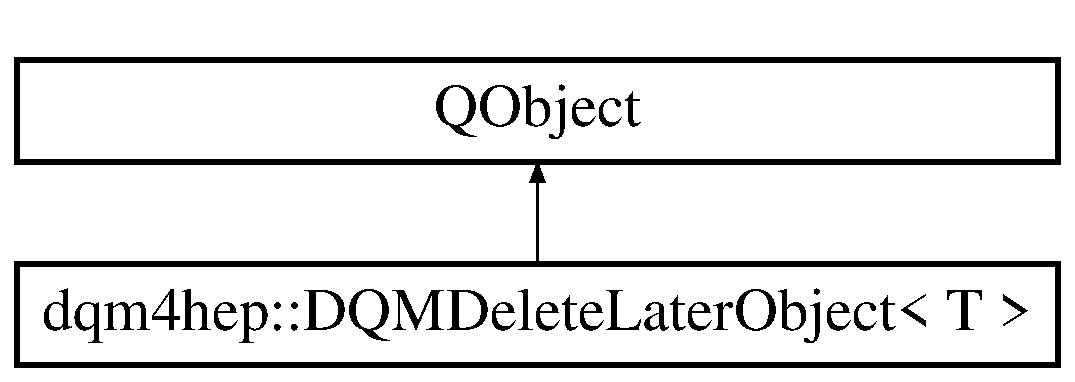
\includegraphics[height=2.000000cm]{classdqm4hep_1_1DQMDeleteLaterObject}
\end{center}
\end{figure}
\subsection*{Public Member Functions}
\begin{DoxyCompactItemize}
\item 
{\bf D\+Q\+M\+Delete\+Later\+Object} (T $\ast$p\+Ptr)
\begin{DoxyCompactList}\small\item\em Constructor. \end{DoxyCompactList}\item 
{\bf $\sim$\+D\+Q\+M\+Delete\+Later\+Object} ()
\begin{DoxyCompactList}\small\item\em Destructor. \end{DoxyCompactList}\end{DoxyCompactItemize}
\subsection*{Static Public Member Functions}
\begin{DoxyCompactItemize}
\item 
static void {\bf delete\+Later\+Object} (T $\ast$p\+Ptr)
\begin{DoxyCompactList}\small\item\em Delete the object in the qt event loop. \end{DoxyCompactList}\end{DoxyCompactItemize}
\subsection*{Private Attributes}
\begin{DoxyCompactItemize}
\item 
T $\ast$ {\bf m\+\_\+p\+Ptr}
\end{DoxyCompactItemize}


\subsection{Detailed Description}
\subsubsection*{template$<$typename T$>$class dqm4hep\+::\+D\+Q\+M\+Delete\+Later\+Object$<$ T $>$}

\doxyref{D\+Q\+M\+Delete\+Later\+Object}{p.}{classdqm4hep_1_1DQMDeleteLaterObject} class. 

Allows to perform delete\+Later() on non-\/qt object. 

Definition at line 42 of file D\+Q\+M\+Delete\+Later\+Object.\+h.



\subsection{Constructor \& Destructor Documentation}
\index{dqm4hep\+::\+D\+Q\+M\+Delete\+Later\+Object@{dqm4hep\+::\+D\+Q\+M\+Delete\+Later\+Object}!D\+Q\+M\+Delete\+Later\+Object@{D\+Q\+M\+Delete\+Later\+Object}}
\index{D\+Q\+M\+Delete\+Later\+Object@{D\+Q\+M\+Delete\+Later\+Object}!dqm4hep\+::\+D\+Q\+M\+Delete\+Later\+Object@{dqm4hep\+::\+D\+Q\+M\+Delete\+Later\+Object}}
\subsubsection[{D\+Q\+M\+Delete\+Later\+Object}]{\setlength{\rightskip}{0pt plus 5cm}template$<$typename T $>$ {\bf dqm4hep\+::\+D\+Q\+M\+Delete\+Later\+Object}$<$ T $>$\+::{\bf D\+Q\+M\+Delete\+Later\+Object} (
\begin{DoxyParamCaption}
\item[{T $\ast$}]{p\+Ptr}
\end{DoxyParamCaption}
)\hspace{0.3cm}{\ttfamily [inline]}}\label{classdqm4hep_1_1DQMDeleteLaterObject_a79bef4cd5fbbb6f4cebb467d21b38823}


Constructor. 



Definition at line 66 of file D\+Q\+M\+Delete\+Later\+Object.\+h.


\begin{DoxyCode}
66                                                             :
67   m_pPtr(pPtr)
68 \{
69   \textcolor{comment}{/* nop */}
70 \}
\end{DoxyCode}
\index{dqm4hep\+::\+D\+Q\+M\+Delete\+Later\+Object@{dqm4hep\+::\+D\+Q\+M\+Delete\+Later\+Object}!````~D\+Q\+M\+Delete\+Later\+Object@{$\sim$\+D\+Q\+M\+Delete\+Later\+Object}}
\index{````~D\+Q\+M\+Delete\+Later\+Object@{$\sim$\+D\+Q\+M\+Delete\+Later\+Object}!dqm4hep\+::\+D\+Q\+M\+Delete\+Later\+Object@{dqm4hep\+::\+D\+Q\+M\+Delete\+Later\+Object}}
\subsubsection[{$\sim$\+D\+Q\+M\+Delete\+Later\+Object}]{\setlength{\rightskip}{0pt plus 5cm}template$<$typename T $>$ {\bf dqm4hep\+::\+D\+Q\+M\+Delete\+Later\+Object}$<$ T $>$\+::$\sim${\bf D\+Q\+M\+Delete\+Later\+Object} (
\begin{DoxyParamCaption}
{}
\end{DoxyParamCaption}
)\hspace{0.3cm}{\ttfamily [inline]}}\label{classdqm4hep_1_1DQMDeleteLaterObject_a282c9b87f50c8a21241ea6a79f4e11c9}


Destructor. 



Definition at line 75 of file D\+Q\+M\+Delete\+Later\+Object.\+h.


\begin{DoxyCode}
76 \{
77   \textcolor{keyword}{delete} m_pPtr;
78 \}
\end{DoxyCode}


\subsection{Member Function Documentation}
\index{dqm4hep\+::\+D\+Q\+M\+Delete\+Later\+Object@{dqm4hep\+::\+D\+Q\+M\+Delete\+Later\+Object}!delete\+Later\+Object@{delete\+Later\+Object}}
\index{delete\+Later\+Object@{delete\+Later\+Object}!dqm4hep\+::\+D\+Q\+M\+Delete\+Later\+Object@{dqm4hep\+::\+D\+Q\+M\+Delete\+Later\+Object}}
\subsubsection[{delete\+Later\+Object}]{\setlength{\rightskip}{0pt plus 5cm}template$<$typename T $>$ void {\bf dqm4hep\+::\+D\+Q\+M\+Delete\+Later\+Object}$<$ T $>$\+::delete\+Later\+Object (
\begin{DoxyParamCaption}
\item[{T $\ast$}]{p\+Ptr}
\end{DoxyParamCaption}
)\hspace{0.3cm}{\ttfamily [inline]}, {\ttfamily [static]}}\label{classdqm4hep_1_1DQMDeleteLaterObject_a056693f82d545fe2ee2e385248506469}


Delete the object in the qt event loop. 



Definition at line 83 of file D\+Q\+M\+Delete\+Later\+Object.\+h.


\begin{DoxyCode}
84 \{
85   DQMDeleteLaterObject<T> *pDeleteObject = \textcolor{keyword}{new} DQMDeleteLaterObject<T>(pPtr);
86   pDeleteObject->deleteLater();
87 \}
\end{DoxyCode}


\subsection{Member Data Documentation}
\index{dqm4hep\+::\+D\+Q\+M\+Delete\+Later\+Object@{dqm4hep\+::\+D\+Q\+M\+Delete\+Later\+Object}!m\+\_\+p\+Ptr@{m\+\_\+p\+Ptr}}
\index{m\+\_\+p\+Ptr@{m\+\_\+p\+Ptr}!dqm4hep\+::\+D\+Q\+M\+Delete\+Later\+Object@{dqm4hep\+::\+D\+Q\+M\+Delete\+Later\+Object}}
\subsubsection[{m\+\_\+p\+Ptr}]{\setlength{\rightskip}{0pt plus 5cm}template$<$typename T$>$ T$\ast$ {\bf dqm4hep\+::\+D\+Q\+M\+Delete\+Later\+Object}$<$ T $>$\+::m\+\_\+p\+Ptr\hspace{0.3cm}{\ttfamily [private]}}\label{classdqm4hep_1_1DQMDeleteLaterObject_a0f8c55bb011426e2698240fce47270e5}


Definition at line 59 of file D\+Q\+M\+Delete\+Later\+Object.\+h.



The documentation for this class was generated from the following file\+:\begin{DoxyCompactItemize}
\item 
{\bf D\+Q\+M\+Delete\+Later\+Object.\+h}\end{DoxyCompactItemize}

\section{dqm4hep\+:\+:D\+Q\+M\+Gui\+Monitor\+Element Class Reference}
\label{classdqm4hep_1_1DQMGuiMonitorElement}\index{dqm4hep\+::\+D\+Q\+M\+Gui\+Monitor\+Element@{dqm4hep\+::\+D\+Q\+M\+Gui\+Monitor\+Element}}


\doxyref{D\+Q\+M\+Gui\+Monitor\+Element}{p.}{classdqm4hep_1_1DQMGuiMonitorElement} class.  




{\ttfamily \#include $<$D\+Q\+M\+Gui\+Monitor\+Element.\+h$>$}

Inheritance diagram for dqm4hep\+:\+:D\+Q\+M\+Gui\+Monitor\+Element\+:\begin{figure}[H]
\begin{center}
\leavevmode
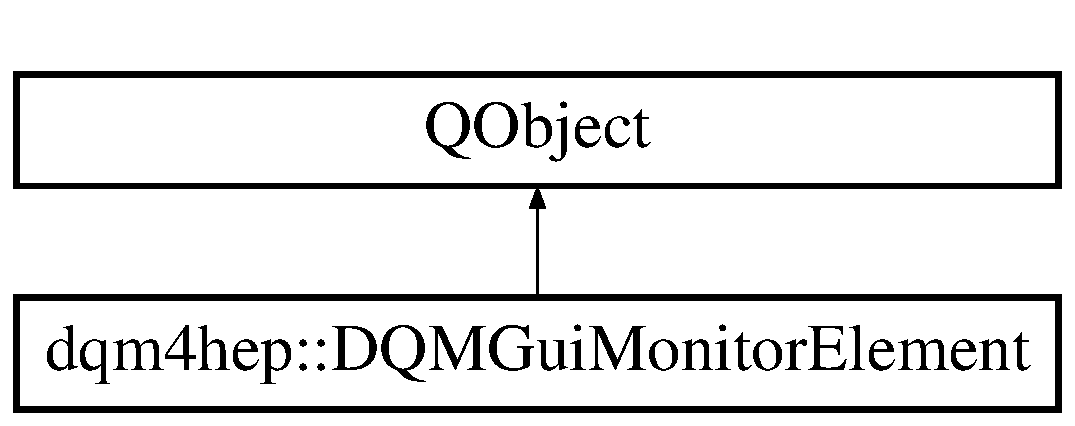
\includegraphics[height=2.000000cm]{classdqm4hep_1_1DQMGuiMonitorElement}
\end{center}
\end{figure}
\subsection*{Signals}
\begin{DoxyCompactItemize}
\item 
void {\bf updated} ()
\begin{DoxyCompactList}\small\item\em Signal emitted when the properties of the monitor element or the monitor element pointer have been updated. \end{DoxyCompactList}\end{DoxyCompactItemize}
\subsection*{Public Member Functions}
\begin{DoxyCompactItemize}
\item 
{\bf D\+Q\+M\+Gui\+Monitor\+Element} (D\+Q\+M\+Monitor\+Element $\ast$p\+Monitor\+Element)
\begin{DoxyCompactList}\small\item\em Constructor with a monitoring instance. \end{DoxyCompactList}\item 
virtual {\bf $\sim$\+D\+Q\+M\+Gui\+Monitor\+Element} ()
\begin{DoxyCompactList}\small\item\em Destructor. \end{DoxyCompactList}\item 
D\+Q\+M\+Monitor\+Element $\ast$ {\bf get\+Monitor\+Element} () const 
\begin{DoxyCompactList}\small\item\em Get the wrapped monitor element. \end{DoxyCompactList}\item 
void {\bf update} (D\+Q\+M\+Monitor\+Element $\ast$p\+Monitor\+Element)
\begin{DoxyCompactList}\small\item\em Update the gui monitor element with a new monitor element. \end{DoxyCompactList}\item 
bool {\bf equals} (D\+Q\+M\+Monitor\+Element $\ast$p\+Monitor\+Element) const 
\begin{DoxyCompactList}\small\item\em Whether the two monitor elements area equal. \end{DoxyCompactList}\item 
bool {\bf equals} ({\bf D\+Q\+M\+Gui\+Monitor\+Element} $\ast$p\+Gui\+Monitor\+Element) const 
\begin{DoxyCompactList}\small\item\em Whether the two monitor elements area equal. \end{DoxyCompactList}\item 
void {\bf set\+Draw\+Option} (const std\+::string \&draw\+Option)
\begin{DoxyCompactList}\small\item\em Set the monitor element draw option. \end{DoxyCompactList}\item 
void {\bf set\+Description} (const std\+::string \&description)
\begin{DoxyCompactList}\small\item\em Set the monitor element description. \end{DoxyCompactList}\item 
void {\bf set\+Quality} (D\+Q\+M\+Quality quality)
\begin{DoxyCompactList}\small\item\em Set the monitor element quality. \end{DoxyCompactList}\end{DoxyCompactItemize}
\subsection*{Protected Attributes}
\begin{DoxyCompactItemize}
\item 
D\+Q\+M\+Monitor\+Element $\ast$ {\bf m\+\_\+p\+Monitor\+Element}
\end{DoxyCompactItemize}
\subsection*{Friends}
\begin{DoxyCompactItemize}
\item 
class {\bf D\+Q\+M\+Monitoring\+Model}
\end{DoxyCompactItemize}


\subsection{Detailed Description}
\doxyref{D\+Q\+M\+Gui\+Monitor\+Element}{p.}{classdqm4hep_1_1DQMGuiMonitorElement} class. 

Definition at line 44 of file D\+Q\+M\+Gui\+Monitor\+Element.\+h.



\subsection{Constructor \& Destructor Documentation}
\index{dqm4hep\+::\+D\+Q\+M\+Gui\+Monitor\+Element@{dqm4hep\+::\+D\+Q\+M\+Gui\+Monitor\+Element}!D\+Q\+M\+Gui\+Monitor\+Element@{D\+Q\+M\+Gui\+Monitor\+Element}}
\index{D\+Q\+M\+Gui\+Monitor\+Element@{D\+Q\+M\+Gui\+Monitor\+Element}!dqm4hep\+::\+D\+Q\+M\+Gui\+Monitor\+Element@{dqm4hep\+::\+D\+Q\+M\+Gui\+Monitor\+Element}}
\subsubsection[{D\+Q\+M\+Gui\+Monitor\+Element}]{\setlength{\rightskip}{0pt plus 5cm}dqm4hep\+::\+D\+Q\+M\+Gui\+Monitor\+Element\+::\+D\+Q\+M\+Gui\+Monitor\+Element (
\begin{DoxyParamCaption}
\item[{D\+Q\+M\+Monitor\+Element $\ast$}]{p\+Monitor\+Element}
\end{DoxyParamCaption}
)}\label{classdqm4hep_1_1DQMGuiMonitorElement_a59fa63814145382885da2d7e671d7fb6}


Constructor with a monitoring instance. 



Definition at line 37 of file D\+Q\+M\+Gui\+Monitor\+Element.\+cc.


\begin{DoxyCode}
37                                                                              :
38     m_pMonitorElement(pMonitorElement)
39 \{
40   \textcolor{comment}{/* nop */}
41 \}
\end{DoxyCode}
\index{dqm4hep\+::\+D\+Q\+M\+Gui\+Monitor\+Element@{dqm4hep\+::\+D\+Q\+M\+Gui\+Monitor\+Element}!````~D\+Q\+M\+Gui\+Monitor\+Element@{$\sim$\+D\+Q\+M\+Gui\+Monitor\+Element}}
\index{````~D\+Q\+M\+Gui\+Monitor\+Element@{$\sim$\+D\+Q\+M\+Gui\+Monitor\+Element}!dqm4hep\+::\+D\+Q\+M\+Gui\+Monitor\+Element@{dqm4hep\+::\+D\+Q\+M\+Gui\+Monitor\+Element}}
\subsubsection[{$\sim$\+D\+Q\+M\+Gui\+Monitor\+Element}]{\setlength{\rightskip}{0pt plus 5cm}dqm4hep\+::\+D\+Q\+M\+Gui\+Monitor\+Element\+::$\sim$\+D\+Q\+M\+Gui\+Monitor\+Element (
\begin{DoxyParamCaption}
{}
\end{DoxyParamCaption}
)\hspace{0.3cm}{\ttfamily [virtual]}}\label{classdqm4hep_1_1DQMGuiMonitorElement_ad65fb15103738425b025c576eb15af25}


Destructor. 



Definition at line 45 of file D\+Q\+M\+Gui\+Monitor\+Element.\+cc.



References m\+\_\+p\+Monitor\+Element.


\begin{DoxyCode}
46 \{
47   \textcolor{keywordflow}{if}(NULL != m_pMonitorElement)
48     \textcolor{keyword}{delete} m_pMonitorElement;
49 \}
\end{DoxyCode}


\subsection{Member Function Documentation}
\index{dqm4hep\+::\+D\+Q\+M\+Gui\+Monitor\+Element@{dqm4hep\+::\+D\+Q\+M\+Gui\+Monitor\+Element}!equals@{equals}}
\index{equals@{equals}!dqm4hep\+::\+D\+Q\+M\+Gui\+Monitor\+Element@{dqm4hep\+::\+D\+Q\+M\+Gui\+Monitor\+Element}}
\subsubsection[{equals}]{\setlength{\rightskip}{0pt plus 5cm}bool dqm4hep\+::\+D\+Q\+M\+Gui\+Monitor\+Element\+::equals (
\begin{DoxyParamCaption}
\item[{D\+Q\+M\+Monitor\+Element $\ast$}]{p\+Monitor\+Element}
\end{DoxyParamCaption}
) const}\label{classdqm4hep_1_1DQMGuiMonitorElement_a40b707b292b5b1d5da4d83a7d045b701}


Whether the two monitor elements area equal. 



Definition at line 77 of file D\+Q\+M\+Gui\+Monitor\+Element.\+cc.



References get\+Monitor\+Element(), and m\+\_\+p\+Monitor\+Element.



Referenced by dqm4hep\+::\+D\+Q\+M\+Canvas\+Area\+::get\+Canvas().


\begin{DoxyCode}
78 \{
79   \textcolor{keywordflow}{if}(NULL == pMonitorElement)
80     \textcolor{keywordflow}{return} \textcolor{keyword}{false};
81 
82   \textcolor{keywordflow}{if}(NULL == m_pMonitorElement)
83     \textcolor{keywordflow}{return} \textcolor{keyword}{false};
84 
85   \textcolor{keyword}{const} DQMPath &path = pMonitorElement->getPath();
86   \textcolor{keyword}{const} std::string &moduleName = pMonitorElement->getModuleName();
87   \textcolor{keyword}{const} std::string &name = pMonitorElement->getName();
88   \textcolor{keyword}{const} std::string &collectorName = pMonitorElement->getCollectorName();
89 
90   \textcolor{keywordtype}{bool} samePath =          (path          == this->getMonitorElement()->getPath());
91   \textcolor{keywordtype}{bool} sameModuleName =    (moduleName    == this->getMonitorElement()->getModuleName());
92   \textcolor{keywordtype}{bool} sameName =          (name          == this->getMonitorElement()->getName());
93   \textcolor{keywordtype}{bool} sameCollectorName = (collectorName == this->getMonitorElement()->getCollectorName());
94 
95   \textcolor{keywordflow}{return} (samePath && sameModuleName && sameName && sameCollectorName);
96 \}
\end{DoxyCode}
\index{dqm4hep\+::\+D\+Q\+M\+Gui\+Monitor\+Element@{dqm4hep\+::\+D\+Q\+M\+Gui\+Monitor\+Element}!equals@{equals}}
\index{equals@{equals}!dqm4hep\+::\+D\+Q\+M\+Gui\+Monitor\+Element@{dqm4hep\+::\+D\+Q\+M\+Gui\+Monitor\+Element}}
\subsubsection[{equals}]{\setlength{\rightskip}{0pt plus 5cm}bool dqm4hep\+::\+D\+Q\+M\+Gui\+Monitor\+Element\+::equals (
\begin{DoxyParamCaption}
\item[{{\bf D\+Q\+M\+Gui\+Monitor\+Element} $\ast$}]{p\+Gui\+Monitor\+Element}
\end{DoxyParamCaption}
) const}\label{classdqm4hep_1_1DQMGuiMonitorElement_a95931d980c4e5c646d1d73db88aad265}


Whether the two monitor elements area equal. 



Definition at line 100 of file D\+Q\+M\+Gui\+Monitor\+Element.\+cc.



References get\+Monitor\+Element().


\begin{DoxyCode}
101 \{
102   \textcolor{keywordflow}{if}(NULL == pGuiMonitorElement)
103     \textcolor{keywordflow}{return} \textcolor{keyword}{false};
104 
105   \textcolor{keyword}{const} DQMPath &path = pGuiMonitorElement->getMonitorElement()->getPath();
106   \textcolor{keyword}{const} std::string &moduleName = pGuiMonitorElement->getMonitorElement()->getModuleName();
107   \textcolor{keyword}{const} std::string &name = pGuiMonitorElement->getMonitorElement()->getName();
108   \textcolor{keyword}{const} std::string &collectorName = pGuiMonitorElement->getMonitorElement()->getCollectorName();
109 
110   \textcolor{keywordtype}{bool} samePath =          (path          == this->getMonitorElement()->getPath());
111   \textcolor{keywordtype}{bool} sameModuleName =    (moduleName    == this->getMonitorElement()->getModuleName());
112   \textcolor{keywordtype}{bool} sameName =          (name          == this->getMonitorElement()->getName());
113   \textcolor{keywordtype}{bool} sameCollectorName = (collectorName == this->getMonitorElement()->getCollectorName());
114 
115   \textcolor{keywordflow}{return} (samePath && sameModuleName && sameName && sameCollectorName);
116 \}
\end{DoxyCode}
\index{dqm4hep\+::\+D\+Q\+M\+Gui\+Monitor\+Element@{dqm4hep\+::\+D\+Q\+M\+Gui\+Monitor\+Element}!get\+Monitor\+Element@{get\+Monitor\+Element}}
\index{get\+Monitor\+Element@{get\+Monitor\+Element}!dqm4hep\+::\+D\+Q\+M\+Gui\+Monitor\+Element@{dqm4hep\+::\+D\+Q\+M\+Gui\+Monitor\+Element}}
\subsubsection[{get\+Monitor\+Element}]{\setlength{\rightskip}{0pt plus 5cm}D\+Q\+M\+Monitor\+Element $\ast$ dqm4hep\+::\+D\+Q\+M\+Gui\+Monitor\+Element\+::get\+Monitor\+Element (
\begin{DoxyParamCaption}
{}
\end{DoxyParamCaption}
) const}\label{classdqm4hep_1_1DQMGuiMonitorElement_a0afc53853489742a5a6256c9945d8593}


Get the wrapped monitor element. 



Definition at line 120 of file D\+Q\+M\+Gui\+Monitor\+Element.\+cc.



References m\+\_\+p\+Monitor\+Element.



Referenced by dqm4hep\+::\+D\+Q\+M\+Root\+Widget\+::draw(), equals(), dqm4hep\+::\+D\+Q\+M\+Monitor\+Element\+Info\+Widget\+::fill\+Infos(), dqm4hep\+::\+D\+Q\+M\+Monitoring\+Model\+::find\+Monitor\+Element(), dqm4hep\+::\+D\+Q\+M\+Monitoring\+Model\+::get\+Or\+Create\+Gui\+Monitor\+Element(), dqm4hep\+::\+D\+Q\+M\+Monitoring\+Model\+::load\+Monitor\+Element\+Info\+List(), dqm4hep\+::\+D\+Q\+M\+Monitoring\+Controller\+::open\+In\+R\+O\+O\+T\+Window(), dqm4hep\+::\+D\+Q\+M\+Monitoring\+Controller\+::open\+Monitor\+Element\+Info(), dqm4hep\+::\+D\+Q\+M\+Monitoring\+Controller\+::open\+Quality\+Test\+Results(), dqm4hep\+::\+D\+Q\+M\+Monitoring\+Controller\+::query\+Update(), dqm4hep\+::\+D\+Q\+M\+Monitor\+Element\+Navigator\+::remove\+Monitor\+Element(), dqm4hep\+::\+D\+Q\+M\+Monitor\+Element\+View\+::remove\+Monitor\+Element(), dqm4hep\+::\+D\+Q\+M\+Monitoring\+Controller\+::save\+As(), dqm4hep\+::\+D\+Q\+M\+Root\+Widget\+::set\+Draw\+Option\+From\+Dialog(), dqm4hep\+::\+D\+Q\+M\+Canvas\+View\+::to\+Xml(), dqm4hep\+::\+D\+Q\+M\+Root\+Widget\+::unzoom(), dqm4hep\+::\+D\+Q\+M\+Monitoring\+Model\+::update\+Monitor\+Element(), dqm4hep\+::\+D\+Q\+M\+Monitor\+Element\+Navigator\+::update\+Monitor\+Element(), dqm4hep\+::\+D\+Q\+M\+Root\+Widget\+::update\+Monitor\+Element(), and dqm4hep\+::\+D\+Q\+M\+Monitor\+Element\+View\+::update\+Monitor\+Element().


\begin{DoxyCode}
121 \{
122   \textcolor{keywordflow}{return} m_pMonitorElement;
123 \}
\end{DoxyCode}
\index{dqm4hep\+::\+D\+Q\+M\+Gui\+Monitor\+Element@{dqm4hep\+::\+D\+Q\+M\+Gui\+Monitor\+Element}!set\+Description@{set\+Description}}
\index{set\+Description@{set\+Description}!dqm4hep\+::\+D\+Q\+M\+Gui\+Monitor\+Element@{dqm4hep\+::\+D\+Q\+M\+Gui\+Monitor\+Element}}
\subsubsection[{set\+Description}]{\setlength{\rightskip}{0pt plus 5cm}void dqm4hep\+::\+D\+Q\+M\+Gui\+Monitor\+Element\+::set\+Description (
\begin{DoxyParamCaption}
\item[{const std\+::string \&}]{description}
\end{DoxyParamCaption}
)}\label{classdqm4hep_1_1DQMGuiMonitorElement_ae3037e21108ed1b5b3429b11a911a2e1}


Set the monitor element description. 



Definition at line 138 of file D\+Q\+M\+Gui\+Monitor\+Element.\+cc.



References m\+\_\+p\+Monitor\+Element, and updated().


\begin{DoxyCode}
139 \{
140   \textcolor{keywordflow}{if}(m_pMonitorElement)
141   \{
142     m_pMonitorElement->setDescription(description);
143     emit updated();
144   \}
145 \}
\end{DoxyCode}
\index{dqm4hep\+::\+D\+Q\+M\+Gui\+Monitor\+Element@{dqm4hep\+::\+D\+Q\+M\+Gui\+Monitor\+Element}!set\+Draw\+Option@{set\+Draw\+Option}}
\index{set\+Draw\+Option@{set\+Draw\+Option}!dqm4hep\+::\+D\+Q\+M\+Gui\+Monitor\+Element@{dqm4hep\+::\+D\+Q\+M\+Gui\+Monitor\+Element}}
\subsubsection[{set\+Draw\+Option}]{\setlength{\rightskip}{0pt plus 5cm}void dqm4hep\+::\+D\+Q\+M\+Gui\+Monitor\+Element\+::set\+Draw\+Option (
\begin{DoxyParamCaption}
\item[{const std\+::string \&}]{draw\+Option}
\end{DoxyParamCaption}
)}\label{classdqm4hep_1_1DQMGuiMonitorElement_a3129237f0eb393d5ba39f421bf68382a}


Set the monitor element draw option. 



Definition at line 127 of file D\+Q\+M\+Gui\+Monitor\+Element.\+cc.



References m\+\_\+p\+Monitor\+Element, and updated().



Referenced by dqm4hep\+::\+D\+Q\+M\+Root\+Widget\+::set\+Draw\+Option(), and dqm4hep\+::\+D\+Q\+M\+Root\+Widget\+::set\+Draw\+Option\+From\+Dialog().


\begin{DoxyCode}
128 \{
129   \textcolor{keywordflow}{if}(m_pMonitorElement)
130   \{
131     m_pMonitorElement->setDrawOption(drawOption);
132     emit updated();
133   \}
134 \}
\end{DoxyCode}
\index{dqm4hep\+::\+D\+Q\+M\+Gui\+Monitor\+Element@{dqm4hep\+::\+D\+Q\+M\+Gui\+Monitor\+Element}!set\+Quality@{set\+Quality}}
\index{set\+Quality@{set\+Quality}!dqm4hep\+::\+D\+Q\+M\+Gui\+Monitor\+Element@{dqm4hep\+::\+D\+Q\+M\+Gui\+Monitor\+Element}}
\subsubsection[{set\+Quality}]{\setlength{\rightskip}{0pt plus 5cm}void dqm4hep\+::\+D\+Q\+M\+Gui\+Monitor\+Element\+::set\+Quality (
\begin{DoxyParamCaption}
\item[{D\+Q\+M\+Quality}]{quality}
\end{DoxyParamCaption}
)}\label{classdqm4hep_1_1DQMGuiMonitorElement_a67010c40d1c798d3e359115eb87cecf9}


Set the monitor element quality. 



Definition at line 149 of file D\+Q\+M\+Gui\+Monitor\+Element.\+cc.



References m\+\_\+p\+Monitor\+Element, and updated().


\begin{DoxyCode}
150 \{
151   \textcolor{keywordflow}{if}(m_pMonitorElement)
152   \{
153     m_pMonitorElement->setQuality(quality);
154     emit updated();
155   \}
156 \}
\end{DoxyCode}
\index{dqm4hep\+::\+D\+Q\+M\+Gui\+Monitor\+Element@{dqm4hep\+::\+D\+Q\+M\+Gui\+Monitor\+Element}!update@{update}}
\index{update@{update}!dqm4hep\+::\+D\+Q\+M\+Gui\+Monitor\+Element@{dqm4hep\+::\+D\+Q\+M\+Gui\+Monitor\+Element}}
\subsubsection[{update}]{\setlength{\rightskip}{0pt plus 5cm}void dqm4hep\+::\+D\+Q\+M\+Gui\+Monitor\+Element\+::update (
\begin{DoxyParamCaption}
\item[{D\+Q\+M\+Monitor\+Element $\ast$}]{p\+Monitor\+Element}
\end{DoxyParamCaption}
)}\label{classdqm4hep_1_1DQMGuiMonitorElement_a9223bec53b3f34ac12f032bc6b1cbf37}


Update the gui monitor element with a new monitor element. 



Definition at line 53 of file D\+Q\+M\+Gui\+Monitor\+Element.\+cc.



References m\+\_\+p\+Monitor\+Element, and updated().



Referenced by dqm4hep\+::\+D\+Q\+M\+Monitoring\+Model\+::update\+Monitor\+Element().


\begin{DoxyCode}
54 \{
55   \textcolor{keywordflow}{if}(m_pMonitorElement == pMonitorElement)
56     \textcolor{keywordflow}{return};
57 
58   \textcolor{keywordflow}{if}(m_pMonitorElement)
59   \{
60     \textcolor{keywordflow}{if}(pMonitorElement)
61     \{
62       \textcolor{comment}{// save previous state}
63       \textcolor{keyword}{const} std::string &drawOption(m_pMonitorElement->getDrawOption());
64       pMonitorElement->setDrawOption(drawOption);
65     \}
66 
67     \textcolor{keyword}{delete} m_pMonitorElement;
68   \}
69 
70   m_pMonitorElement = pMonitorElement;
71 
72   emit updated();
73 \}
\end{DoxyCode}
\index{dqm4hep\+::\+D\+Q\+M\+Gui\+Monitor\+Element@{dqm4hep\+::\+D\+Q\+M\+Gui\+Monitor\+Element}!updated@{updated}}
\index{updated@{updated}!dqm4hep\+::\+D\+Q\+M\+Gui\+Monitor\+Element@{dqm4hep\+::\+D\+Q\+M\+Gui\+Monitor\+Element}}
\subsubsection[{updated}]{\setlength{\rightskip}{0pt plus 5cm}void dqm4hep\+::\+D\+Q\+M\+Gui\+Monitor\+Element\+::updated (
\begin{DoxyParamCaption}
{}
\end{DoxyParamCaption}
)\hspace{0.3cm}{\ttfamily [signal]}}\label{classdqm4hep_1_1DQMGuiMonitorElement_a1c6ff9ed1c7f6801bb801cc9391c382c}


Signal emitted when the properties of the monitor element or the monitor element pointer have been updated. 



Referenced by set\+Description(), set\+Draw\+Option(), set\+Quality(), and update().



\subsection{Friends And Related Function Documentation}
\index{dqm4hep\+::\+D\+Q\+M\+Gui\+Monitor\+Element@{dqm4hep\+::\+D\+Q\+M\+Gui\+Monitor\+Element}!D\+Q\+M\+Monitoring\+Model@{D\+Q\+M\+Monitoring\+Model}}
\index{D\+Q\+M\+Monitoring\+Model@{D\+Q\+M\+Monitoring\+Model}!dqm4hep\+::\+D\+Q\+M\+Gui\+Monitor\+Element@{dqm4hep\+::\+D\+Q\+M\+Gui\+Monitor\+Element}}
\subsubsection[{D\+Q\+M\+Monitoring\+Model}]{\setlength{\rightskip}{0pt plus 5cm}friend class {\bf D\+Q\+M\+Monitoring\+Model}\hspace{0.3cm}{\ttfamily [friend]}}\label{classdqm4hep_1_1DQMGuiMonitorElement_a92a78e9a4fe4db0a72840a4de5b98066}


Definition at line 48 of file D\+Q\+M\+Gui\+Monitor\+Element.\+h.



\subsection{Member Data Documentation}
\index{dqm4hep\+::\+D\+Q\+M\+Gui\+Monitor\+Element@{dqm4hep\+::\+D\+Q\+M\+Gui\+Monitor\+Element}!m\+\_\+p\+Monitor\+Element@{m\+\_\+p\+Monitor\+Element}}
\index{m\+\_\+p\+Monitor\+Element@{m\+\_\+p\+Monitor\+Element}!dqm4hep\+::\+D\+Q\+M\+Gui\+Monitor\+Element@{dqm4hep\+::\+D\+Q\+M\+Gui\+Monitor\+Element}}
\subsubsection[{m\+\_\+p\+Monitor\+Element}]{\setlength{\rightskip}{0pt plus 5cm}D\+Q\+M\+Monitor\+Element$\ast$ dqm4hep\+::\+D\+Q\+M\+Gui\+Monitor\+Element\+::m\+\_\+p\+Monitor\+Element\hspace{0.3cm}{\ttfamily [protected]}}\label{classdqm4hep_1_1DQMGuiMonitorElement_aec7a7ced57453f623eebd7a21854d361}


Definition at line 94 of file D\+Q\+M\+Gui\+Monitor\+Element.\+h.



Referenced by equals(), get\+Monitor\+Element(), set\+Description(), set\+Draw\+Option(), set\+Quality(), update(), and $\sim$\+D\+Q\+M\+Gui\+Monitor\+Element().



The documentation for this class was generated from the following files\+:\begin{DoxyCompactItemize}
\item 
{\bf D\+Q\+M\+Gui\+Monitor\+Element.\+h}\item 
{\bf D\+Q\+M\+Gui\+Monitor\+Element.\+cc}\end{DoxyCompactItemize}

\section{dqm4hep\+:\+:D\+Q\+M\+Gui\+Monitor\+Element\+Client Class Reference}
\label{classdqm4hep_1_1DQMGuiMonitorElementClient}\index{dqm4hep\+::\+D\+Q\+M\+Gui\+Monitor\+Element\+Client@{dqm4hep\+::\+D\+Q\+M\+Gui\+Monitor\+Element\+Client}}


\doxyref{D\+Q\+M\+Gui\+Monitor\+Element\+Client}{p.}{classdqm4hep_1_1DQMGuiMonitorElementClient} class.  




{\ttfamily \#include $<$D\+Q\+M\+Gui\+Monitor\+Element\+Client.\+h$>$}

Inheritance diagram for dqm4hep\+:\+:D\+Q\+M\+Gui\+Monitor\+Element\+Client\+:\begin{figure}[H]
\begin{center}
\leavevmode
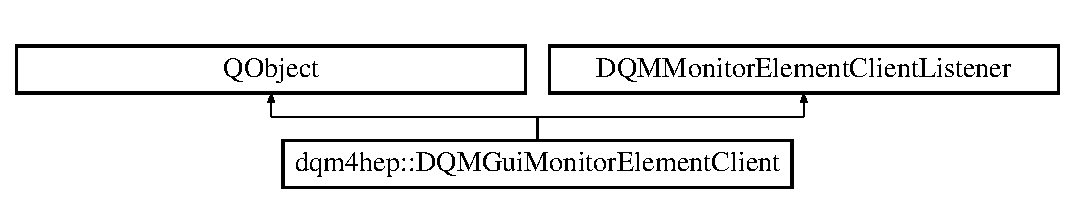
\includegraphics[height=2.000000cm]{classdqm4hep_1_1DQMGuiMonitorElementClient}
\end{center}
\end{figure}
\subsection*{Signals}
\begin{DoxyCompactItemize}
\item 
void {\bf collector\+Info\+Received} (const D\+Q\+M\+Collector\+Info \&)
\begin{DoxyCompactList}\small\item\em Qt signal emitted when the dim handler receives a collector info structure. \end{DoxyCompactList}\item 
void {\bf monitor\+Element\+List\+Name\+Received} (const D\+Q\+M\+Monitor\+Element\+Info\+List \&)
\begin{DoxyCompactList}\small\item\em Qt signal emitted when the dim handler receives an info list on monitor elements. \end{DoxyCompactList}\item 
void {\bf monitor\+Element\+Publication\+Received} (const D\+Q\+M\+Monitor\+Element\+Publication \&)
\begin{DoxyCompactList}\small\item\em Qt signal emitted when the dim handler receives a monitor element publication. \end{DoxyCompactList}\item 
void {\bf on\+Monitor\+Element\+Client\+Connect} ()
\begin{DoxyCompactList}\small\item\em Qt signal emitted when the client is connected. \end{DoxyCompactList}\item 
void {\bf on\+Monitor\+Element\+Client\+Disconnect} ()
\begin{DoxyCompactList}\small\item\em Qt signal emitted when the client is disconnected. \end{DoxyCompactList}\item 
void {\bf on\+Server\+Startup} ()
\begin{DoxyCompactList}\small\item\em Qt signal emitted when the collector server is started. \end{DoxyCompactList}\item 
void {\bf on\+Server\+Shutdown} ()
\begin{DoxyCompactList}\small\item\em Qt signal emitted when the collector server is shut down. \end{DoxyCompactList}\end{DoxyCompactItemize}
\subsection*{Public Member Functions}
\begin{DoxyCompactItemize}
\item 
{\bf D\+Q\+M\+Gui\+Monitor\+Element\+Client} (const std\+::string \&collector\+Name)
\begin{DoxyCompactList}\small\item\em Constructor. \end{DoxyCompactList}\item 
virtual {\bf $\sim$\+D\+Q\+M\+Gui\+Monitor\+Element\+Client} ()
\begin{DoxyCompactList}\small\item\em Destructor. \end{DoxyCompactList}\item 
D\+Q\+M\+Monitor\+Element\+Client $\ast$ {\bf get\+Monitor\+Element\+Client} () const 
\begin{DoxyCompactList}\small\item\em Get the monitor element client instance (dqm core class) \end{DoxyCompactList}\end{DoxyCompactItemize}
\subsection*{Private Member Functions}
\begin{DoxyCompactItemize}
\item 
void {\bf on\+Monitor\+Element\+Client\+Connect} (D\+Q\+M\+Monitor\+Element\+Client $\ast$)
\item 
void {\bf on\+Monitor\+Element\+Client\+Disconnect} (D\+Q\+M\+Monitor\+Element\+Client $\ast$)
\item 
void {\bf on\+Server\+Startup} (D\+Q\+M\+Monitor\+Element\+Client $\ast$)
\item 
void {\bf on\+Server\+Shutdown} (D\+Q\+M\+Monitor\+Element\+Client $\ast$)
\item 
void {\bf available\+Monitor\+Element\+List\+Received} (D\+Q\+M\+Monitor\+Element\+Client $\ast$, const D\+Q\+M\+Monitor\+Element\+Info\+List \&)
\item 
void {\bf monitor\+Element\+Collector\+Info\+Received} (D\+Q\+M\+Monitor\+Element\+Client $\ast$, const D\+Q\+M\+Collector\+Info \&)
\item 
void {\bf monitor\+Elements\+Received} (D\+Q\+M\+Monitor\+Element\+Client $\ast$, D\+Q\+M\+Monitor\+Element\+Publication \&)
\end{DoxyCompactItemize}
\subsection*{Private Attributes}
\begin{DoxyCompactItemize}
\item 
D\+Q\+M\+Monitor\+Element\+Client $\ast$ {\bf m\+\_\+p\+Monitor\+Element\+Client}
\item 
D\+Q\+M\+Monitor\+Element\+Publication {\bf m\+\_\+publication}
\end{DoxyCompactItemize}


\subsection{Detailed Description}
\doxyref{D\+Q\+M\+Gui\+Monitor\+Element\+Client}{p.}{classdqm4hep_1_1DQMGuiMonitorElementClient} class. 

Definition at line 42 of file D\+Q\+M\+Gui\+Monitor\+Element\+Client.\+h.



\subsection{Constructor \& Destructor Documentation}
\index{dqm4hep\+::\+D\+Q\+M\+Gui\+Monitor\+Element\+Client@{dqm4hep\+::\+D\+Q\+M\+Gui\+Monitor\+Element\+Client}!D\+Q\+M\+Gui\+Monitor\+Element\+Client@{D\+Q\+M\+Gui\+Monitor\+Element\+Client}}
\index{D\+Q\+M\+Gui\+Monitor\+Element\+Client@{D\+Q\+M\+Gui\+Monitor\+Element\+Client}!dqm4hep\+::\+D\+Q\+M\+Gui\+Monitor\+Element\+Client@{dqm4hep\+::\+D\+Q\+M\+Gui\+Monitor\+Element\+Client}}
\subsubsection[{D\+Q\+M\+Gui\+Monitor\+Element\+Client}]{\setlength{\rightskip}{0pt plus 5cm}dqm4hep\+::\+D\+Q\+M\+Gui\+Monitor\+Element\+Client\+::\+D\+Q\+M\+Gui\+Monitor\+Element\+Client (
\begin{DoxyParamCaption}
\item[{const std\+::string \&}]{collector\+Name}
\end{DoxyParamCaption}
)}\label{classdqm4hep_1_1DQMGuiMonitorElementClient_a7f3838ba6f21b205eaf7ab04084e5f0a}


Constructor. 



Definition at line 34 of file D\+Q\+M\+Gui\+Monitor\+Element\+Client.\+cc.



References m\+\_\+p\+Monitor\+Element\+Client.


\begin{DoxyCode}
34                                                                                      :
35     m_pMonitorElementClient(NULL)
36 \{
37   m_pMonitorElementClient = \textcolor{keyword}{new} DQMMonitorElementClient();
38   m_pMonitorElementClient->addListener(\textcolor{keyword}{this});
39   m_pMonitorElementClient->setCollectorName(collectorName);
40 \}
\end{DoxyCode}
\index{dqm4hep\+::\+D\+Q\+M\+Gui\+Monitor\+Element\+Client@{dqm4hep\+::\+D\+Q\+M\+Gui\+Monitor\+Element\+Client}!````~D\+Q\+M\+Gui\+Monitor\+Element\+Client@{$\sim$\+D\+Q\+M\+Gui\+Monitor\+Element\+Client}}
\index{````~D\+Q\+M\+Gui\+Monitor\+Element\+Client@{$\sim$\+D\+Q\+M\+Gui\+Monitor\+Element\+Client}!dqm4hep\+::\+D\+Q\+M\+Gui\+Monitor\+Element\+Client@{dqm4hep\+::\+D\+Q\+M\+Gui\+Monitor\+Element\+Client}}
\subsubsection[{$\sim$\+D\+Q\+M\+Gui\+Monitor\+Element\+Client}]{\setlength{\rightskip}{0pt plus 5cm}dqm4hep\+::\+D\+Q\+M\+Gui\+Monitor\+Element\+Client\+::$\sim$\+D\+Q\+M\+Gui\+Monitor\+Element\+Client (
\begin{DoxyParamCaption}
{}
\end{DoxyParamCaption}
)\hspace{0.3cm}{\ttfamily [virtual]}}\label{classdqm4hep_1_1DQMGuiMonitorElementClient_a9b6118c118f30c9e74fe272e77301260}


Destructor. 



Definition at line 44 of file D\+Q\+M\+Gui\+Monitor\+Element\+Client.\+cc.



References m\+\_\+p\+Monitor\+Element\+Client.


\begin{DoxyCode}
45 \{
46   \textcolor{keyword}{delete} m_pMonitorElementClient;
47 \}
\end{DoxyCode}


\subsection{Member Function Documentation}
\index{dqm4hep\+::\+D\+Q\+M\+Gui\+Monitor\+Element\+Client@{dqm4hep\+::\+D\+Q\+M\+Gui\+Monitor\+Element\+Client}!available\+Monitor\+Element\+List\+Received@{available\+Monitor\+Element\+List\+Received}}
\index{available\+Monitor\+Element\+List\+Received@{available\+Monitor\+Element\+List\+Received}!dqm4hep\+::\+D\+Q\+M\+Gui\+Monitor\+Element\+Client@{dqm4hep\+::\+D\+Q\+M\+Gui\+Monitor\+Element\+Client}}
\subsubsection[{available\+Monitor\+Element\+List\+Received}]{\setlength{\rightskip}{0pt plus 5cm}void dqm4hep\+::\+D\+Q\+M\+Gui\+Monitor\+Element\+Client\+::available\+Monitor\+Element\+List\+Received (
\begin{DoxyParamCaption}
\item[{D\+Q\+M\+Monitor\+Element\+Client $\ast$}]{, }
\item[{const D\+Q\+M\+Monitor\+Element\+Info\+List \&}]{info\+List}
\end{DoxyParamCaption}
)\hspace{0.3cm}{\ttfamily [private]}}\label{classdqm4hep_1_1DQMGuiMonitorElementClient_afadd33d7c31ed8f5b4919fefef5f1e05}


Definition at line 65 of file D\+Q\+M\+Gui\+Monitor\+Element\+Client.\+cc.



References monitor\+Element\+List\+Name\+Received().


\begin{DoxyCode}
66 \{
67   emit monitorElementListNameReceived(infoList);
68 \}
\end{DoxyCode}
\index{dqm4hep\+::\+D\+Q\+M\+Gui\+Monitor\+Element\+Client@{dqm4hep\+::\+D\+Q\+M\+Gui\+Monitor\+Element\+Client}!collector\+Info\+Received@{collector\+Info\+Received}}
\index{collector\+Info\+Received@{collector\+Info\+Received}!dqm4hep\+::\+D\+Q\+M\+Gui\+Monitor\+Element\+Client@{dqm4hep\+::\+D\+Q\+M\+Gui\+Monitor\+Element\+Client}}
\subsubsection[{collector\+Info\+Received}]{\setlength{\rightskip}{0pt plus 5cm}void dqm4hep\+::\+D\+Q\+M\+Gui\+Monitor\+Element\+Client\+::collector\+Info\+Received (
\begin{DoxyParamCaption}
\item[{const D\+Q\+M\+Collector\+Info \&}]{}
\end{DoxyParamCaption}
)\hspace{0.3cm}{\ttfamily [signal]}}\label{classdqm4hep_1_1DQMGuiMonitorElementClient_a28de411f61b6b7316e37095c6b3757c0}


Qt signal emitted when the dim handler receives a collector info structure. 



Referenced by monitor\+Element\+Collector\+Info\+Received().

\index{dqm4hep\+::\+D\+Q\+M\+Gui\+Monitor\+Element\+Client@{dqm4hep\+::\+D\+Q\+M\+Gui\+Monitor\+Element\+Client}!get\+Monitor\+Element\+Client@{get\+Monitor\+Element\+Client}}
\index{get\+Monitor\+Element\+Client@{get\+Monitor\+Element\+Client}!dqm4hep\+::\+D\+Q\+M\+Gui\+Monitor\+Element\+Client@{dqm4hep\+::\+D\+Q\+M\+Gui\+Monitor\+Element\+Client}}
\subsubsection[{get\+Monitor\+Element\+Client}]{\setlength{\rightskip}{0pt plus 5cm}D\+Q\+M\+Monitor\+Element\+Client $\ast$ dqm4hep\+::\+D\+Q\+M\+Gui\+Monitor\+Element\+Client\+::get\+Monitor\+Element\+Client (
\begin{DoxyParamCaption}
{}
\end{DoxyParamCaption}
) const}\label{classdqm4hep_1_1DQMGuiMonitorElementClient_a6eaf5a063d6a62c3098fa284a4b28706}


Get the monitor element client instance (dqm core class) 



Definition at line 51 of file D\+Q\+M\+Gui\+Monitor\+Element\+Client.\+cc.



References m\+\_\+p\+Monitor\+Element\+Client.



Referenced by dqm4hep\+::\+D\+Q\+M\+Browser\+Widget\+::handle\+Collector\+Selection(), dqm4hep\+::\+D\+Q\+M\+Monitoring\+Controller\+::handle\+Server\+Shutdown(), dqm4hep\+::\+D\+Q\+M\+Monitoring\+Controller\+::handle\+Server\+Startup(), dqm4hep\+::\+D\+Q\+M\+Browser\+Widget\+::query\+Search(), dqm4hep\+::\+D\+Q\+M\+Monitoring\+Controller\+::query\+Subscribed\+Monitor\+Elements(), dqm4hep\+::\+D\+Q\+M\+Monitoring\+Controller\+::subscribe(), and dqm4hep\+::\+D\+Q\+M\+Monitoring\+Controller\+::unsubscribe().


\begin{DoxyCode}
52 \{
53   \textcolor{keywordflow}{return} m_pMonitorElementClient;
54 \}
\end{DoxyCode}
\index{dqm4hep\+::\+D\+Q\+M\+Gui\+Monitor\+Element\+Client@{dqm4hep\+::\+D\+Q\+M\+Gui\+Monitor\+Element\+Client}!monitor\+Element\+Collector\+Info\+Received@{monitor\+Element\+Collector\+Info\+Received}}
\index{monitor\+Element\+Collector\+Info\+Received@{monitor\+Element\+Collector\+Info\+Received}!dqm4hep\+::\+D\+Q\+M\+Gui\+Monitor\+Element\+Client@{dqm4hep\+::\+D\+Q\+M\+Gui\+Monitor\+Element\+Client}}
\subsubsection[{monitor\+Element\+Collector\+Info\+Received}]{\setlength{\rightskip}{0pt plus 5cm}void dqm4hep\+::\+D\+Q\+M\+Gui\+Monitor\+Element\+Client\+::monitor\+Element\+Collector\+Info\+Received (
\begin{DoxyParamCaption}
\item[{D\+Q\+M\+Monitor\+Element\+Client $\ast$}]{, }
\item[{const D\+Q\+M\+Collector\+Info \&}]{collector\+Info}
\end{DoxyParamCaption}
)\hspace{0.3cm}{\ttfamily [private]}}\label{classdqm4hep_1_1DQMGuiMonitorElementClient_a12b8e824b375344a967b7c568894ef06}


Definition at line 58 of file D\+Q\+M\+Gui\+Monitor\+Element\+Client.\+cc.



References collector\+Info\+Received().


\begin{DoxyCode}
59 \{
60   emit collectorInfoReceived(collectorInfo);
61 \}
\end{DoxyCode}
\index{dqm4hep\+::\+D\+Q\+M\+Gui\+Monitor\+Element\+Client@{dqm4hep\+::\+D\+Q\+M\+Gui\+Monitor\+Element\+Client}!monitor\+Element\+List\+Name\+Received@{monitor\+Element\+List\+Name\+Received}}
\index{monitor\+Element\+List\+Name\+Received@{monitor\+Element\+List\+Name\+Received}!dqm4hep\+::\+D\+Q\+M\+Gui\+Monitor\+Element\+Client@{dqm4hep\+::\+D\+Q\+M\+Gui\+Monitor\+Element\+Client}}
\subsubsection[{monitor\+Element\+List\+Name\+Received}]{\setlength{\rightskip}{0pt plus 5cm}void dqm4hep\+::\+D\+Q\+M\+Gui\+Monitor\+Element\+Client\+::monitor\+Element\+List\+Name\+Received (
\begin{DoxyParamCaption}
\item[{const D\+Q\+M\+Monitor\+Element\+Info\+List \&}]{}
\end{DoxyParamCaption}
)\hspace{0.3cm}{\ttfamily [signal]}}\label{classdqm4hep_1_1DQMGuiMonitorElementClient_a204565410ba871032495a8c80cfa7105}


Qt signal emitted when the dim handler receives an info list on monitor elements. 



Referenced by available\+Monitor\+Element\+List\+Received().

\index{dqm4hep\+::\+D\+Q\+M\+Gui\+Monitor\+Element\+Client@{dqm4hep\+::\+D\+Q\+M\+Gui\+Monitor\+Element\+Client}!monitor\+Element\+Publication\+Received@{monitor\+Element\+Publication\+Received}}
\index{monitor\+Element\+Publication\+Received@{monitor\+Element\+Publication\+Received}!dqm4hep\+::\+D\+Q\+M\+Gui\+Monitor\+Element\+Client@{dqm4hep\+::\+D\+Q\+M\+Gui\+Monitor\+Element\+Client}}
\subsubsection[{monitor\+Element\+Publication\+Received}]{\setlength{\rightskip}{0pt plus 5cm}void dqm4hep\+::\+D\+Q\+M\+Gui\+Monitor\+Element\+Client\+::monitor\+Element\+Publication\+Received (
\begin{DoxyParamCaption}
\item[{const D\+Q\+M\+Monitor\+Element\+Publication \&}]{}
\end{DoxyParamCaption}
)\hspace{0.3cm}{\ttfamily [signal]}}\label{classdqm4hep_1_1DQMGuiMonitorElementClient_acd6751e8ffb7ddb8a28043703e0d355d}


Qt signal emitted when the dim handler receives a monitor element publication. 



Referenced by monitor\+Elements\+Received().

\index{dqm4hep\+::\+D\+Q\+M\+Gui\+Monitor\+Element\+Client@{dqm4hep\+::\+D\+Q\+M\+Gui\+Monitor\+Element\+Client}!monitor\+Elements\+Received@{monitor\+Elements\+Received}}
\index{monitor\+Elements\+Received@{monitor\+Elements\+Received}!dqm4hep\+::\+D\+Q\+M\+Gui\+Monitor\+Element\+Client@{dqm4hep\+::\+D\+Q\+M\+Gui\+Monitor\+Element\+Client}}
\subsubsection[{monitor\+Elements\+Received}]{\setlength{\rightskip}{0pt plus 5cm}void dqm4hep\+::\+D\+Q\+M\+Gui\+Monitor\+Element\+Client\+::monitor\+Elements\+Received (
\begin{DoxyParamCaption}
\item[{D\+Q\+M\+Monitor\+Element\+Client $\ast$}]{, }
\item[{D\+Q\+M\+Monitor\+Element\+Publication \&}]{publication}
\end{DoxyParamCaption}
)\hspace{0.3cm}{\ttfamily [private]}}\label{classdqm4hep_1_1DQMGuiMonitorElementClient_a23c09dd2b24e3b727e58a8411bb6d2f5}


Definition at line 72 of file D\+Q\+M\+Gui\+Monitor\+Element\+Client.\+cc.



References monitor\+Element\+Publication\+Received().


\begin{DoxyCode}
73 \{
74   \textcolor{comment}{// get copy of publication and clear the one in argument}
75   DQMMonitorElementPublication publicationCopy(publication);
76   publication.clear();
77   emit monitorElementPublicationReceived(publicationCopy);
78 \}
\end{DoxyCode}
\index{dqm4hep\+::\+D\+Q\+M\+Gui\+Monitor\+Element\+Client@{dqm4hep\+::\+D\+Q\+M\+Gui\+Monitor\+Element\+Client}!on\+Monitor\+Element\+Client\+Connect@{on\+Monitor\+Element\+Client\+Connect}}
\index{on\+Monitor\+Element\+Client\+Connect@{on\+Monitor\+Element\+Client\+Connect}!dqm4hep\+::\+D\+Q\+M\+Gui\+Monitor\+Element\+Client@{dqm4hep\+::\+D\+Q\+M\+Gui\+Monitor\+Element\+Client}}
\subsubsection[{on\+Monitor\+Element\+Client\+Connect}]{\setlength{\rightskip}{0pt plus 5cm}void dqm4hep\+::\+D\+Q\+M\+Gui\+Monitor\+Element\+Client\+::on\+Monitor\+Element\+Client\+Connect (
\begin{DoxyParamCaption}
{}
\end{DoxyParamCaption}
)\hspace{0.3cm}{\ttfamily [signal]}}\label{classdqm4hep_1_1DQMGuiMonitorElementClient_a80fb3902011eb4ac86a44bc9bb56605f}


Qt signal emitted when the client is connected. 



Referenced by on\+Monitor\+Element\+Client\+Connect().

\index{dqm4hep\+::\+D\+Q\+M\+Gui\+Monitor\+Element\+Client@{dqm4hep\+::\+D\+Q\+M\+Gui\+Monitor\+Element\+Client}!on\+Monitor\+Element\+Client\+Connect@{on\+Monitor\+Element\+Client\+Connect}}
\index{on\+Monitor\+Element\+Client\+Connect@{on\+Monitor\+Element\+Client\+Connect}!dqm4hep\+::\+D\+Q\+M\+Gui\+Monitor\+Element\+Client@{dqm4hep\+::\+D\+Q\+M\+Gui\+Monitor\+Element\+Client}}
\subsubsection[{on\+Monitor\+Element\+Client\+Connect}]{\setlength{\rightskip}{0pt plus 5cm}void dqm4hep\+::\+D\+Q\+M\+Gui\+Monitor\+Element\+Client\+::on\+Monitor\+Element\+Client\+Connect (
\begin{DoxyParamCaption}
\item[{D\+Q\+M\+Monitor\+Element\+Client $\ast$}]{}
\end{DoxyParamCaption}
)\hspace{0.3cm}{\ttfamily [private]}}\label{classdqm4hep_1_1DQMGuiMonitorElementClient_ace764db279586aca06bfc09c9594a356}


Definition at line 82 of file D\+Q\+M\+Gui\+Monitor\+Element\+Client.\+cc.



References on\+Monitor\+Element\+Client\+Connect().


\begin{DoxyCode}
83 \{
84   emit onMonitorElementClientConnect();
85 \}
\end{DoxyCode}
\index{dqm4hep\+::\+D\+Q\+M\+Gui\+Monitor\+Element\+Client@{dqm4hep\+::\+D\+Q\+M\+Gui\+Monitor\+Element\+Client}!on\+Monitor\+Element\+Client\+Disconnect@{on\+Monitor\+Element\+Client\+Disconnect}}
\index{on\+Monitor\+Element\+Client\+Disconnect@{on\+Monitor\+Element\+Client\+Disconnect}!dqm4hep\+::\+D\+Q\+M\+Gui\+Monitor\+Element\+Client@{dqm4hep\+::\+D\+Q\+M\+Gui\+Monitor\+Element\+Client}}
\subsubsection[{on\+Monitor\+Element\+Client\+Disconnect}]{\setlength{\rightskip}{0pt plus 5cm}void dqm4hep\+::\+D\+Q\+M\+Gui\+Monitor\+Element\+Client\+::on\+Monitor\+Element\+Client\+Disconnect (
\begin{DoxyParamCaption}
{}
\end{DoxyParamCaption}
)\hspace{0.3cm}{\ttfamily [signal]}}\label{classdqm4hep_1_1DQMGuiMonitorElementClient_a04065b4cae54513d54b03d8d705f363f}


Qt signal emitted when the client is disconnected. 



Referenced by on\+Monitor\+Element\+Client\+Disconnect().

\index{dqm4hep\+::\+D\+Q\+M\+Gui\+Monitor\+Element\+Client@{dqm4hep\+::\+D\+Q\+M\+Gui\+Monitor\+Element\+Client}!on\+Monitor\+Element\+Client\+Disconnect@{on\+Monitor\+Element\+Client\+Disconnect}}
\index{on\+Monitor\+Element\+Client\+Disconnect@{on\+Monitor\+Element\+Client\+Disconnect}!dqm4hep\+::\+D\+Q\+M\+Gui\+Monitor\+Element\+Client@{dqm4hep\+::\+D\+Q\+M\+Gui\+Monitor\+Element\+Client}}
\subsubsection[{on\+Monitor\+Element\+Client\+Disconnect}]{\setlength{\rightskip}{0pt plus 5cm}void dqm4hep\+::\+D\+Q\+M\+Gui\+Monitor\+Element\+Client\+::on\+Monitor\+Element\+Client\+Disconnect (
\begin{DoxyParamCaption}
\item[{D\+Q\+M\+Monitor\+Element\+Client $\ast$}]{}
\end{DoxyParamCaption}
)\hspace{0.3cm}{\ttfamily [private]}}\label{classdqm4hep_1_1DQMGuiMonitorElementClient_ae89e31b92a676cffb0cb9e1b29a449ee}


Definition at line 89 of file D\+Q\+M\+Gui\+Monitor\+Element\+Client.\+cc.



References on\+Monitor\+Element\+Client\+Disconnect().


\begin{DoxyCode}
90 \{
91   emit onMonitorElementClientDisconnect();
92 \}
\end{DoxyCode}
\index{dqm4hep\+::\+D\+Q\+M\+Gui\+Monitor\+Element\+Client@{dqm4hep\+::\+D\+Q\+M\+Gui\+Monitor\+Element\+Client}!on\+Server\+Shutdown@{on\+Server\+Shutdown}}
\index{on\+Server\+Shutdown@{on\+Server\+Shutdown}!dqm4hep\+::\+D\+Q\+M\+Gui\+Monitor\+Element\+Client@{dqm4hep\+::\+D\+Q\+M\+Gui\+Monitor\+Element\+Client}}
\subsubsection[{on\+Server\+Shutdown}]{\setlength{\rightskip}{0pt plus 5cm}void dqm4hep\+::\+D\+Q\+M\+Gui\+Monitor\+Element\+Client\+::on\+Server\+Shutdown (
\begin{DoxyParamCaption}
{}
\end{DoxyParamCaption}
)\hspace{0.3cm}{\ttfamily [signal]}}\label{classdqm4hep_1_1DQMGuiMonitorElementClient_adcf32289f2b7eb3b8a1021273b174d60}


Qt signal emitted when the collector server is shut down. 



Referenced by on\+Server\+Shutdown().

\index{dqm4hep\+::\+D\+Q\+M\+Gui\+Monitor\+Element\+Client@{dqm4hep\+::\+D\+Q\+M\+Gui\+Monitor\+Element\+Client}!on\+Server\+Shutdown@{on\+Server\+Shutdown}}
\index{on\+Server\+Shutdown@{on\+Server\+Shutdown}!dqm4hep\+::\+D\+Q\+M\+Gui\+Monitor\+Element\+Client@{dqm4hep\+::\+D\+Q\+M\+Gui\+Monitor\+Element\+Client}}
\subsubsection[{on\+Server\+Shutdown}]{\setlength{\rightskip}{0pt plus 5cm}void dqm4hep\+::\+D\+Q\+M\+Gui\+Monitor\+Element\+Client\+::on\+Server\+Shutdown (
\begin{DoxyParamCaption}
\item[{D\+Q\+M\+Monitor\+Element\+Client $\ast$}]{}
\end{DoxyParamCaption}
)\hspace{0.3cm}{\ttfamily [private]}}\label{classdqm4hep_1_1DQMGuiMonitorElementClient_ac65c02a264e8b5fea0f991e594d27da2}


Definition at line 103 of file D\+Q\+M\+Gui\+Monitor\+Element\+Client.\+cc.



References on\+Server\+Shutdown().


\begin{DoxyCode}
104 \{
105   emit onServerShutdown();
106 \}
\end{DoxyCode}
\index{dqm4hep\+::\+D\+Q\+M\+Gui\+Monitor\+Element\+Client@{dqm4hep\+::\+D\+Q\+M\+Gui\+Monitor\+Element\+Client}!on\+Server\+Startup@{on\+Server\+Startup}}
\index{on\+Server\+Startup@{on\+Server\+Startup}!dqm4hep\+::\+D\+Q\+M\+Gui\+Monitor\+Element\+Client@{dqm4hep\+::\+D\+Q\+M\+Gui\+Monitor\+Element\+Client}}
\subsubsection[{on\+Server\+Startup}]{\setlength{\rightskip}{0pt plus 5cm}void dqm4hep\+::\+D\+Q\+M\+Gui\+Monitor\+Element\+Client\+::on\+Server\+Startup (
\begin{DoxyParamCaption}
{}
\end{DoxyParamCaption}
)\hspace{0.3cm}{\ttfamily [signal]}}\label{classdqm4hep_1_1DQMGuiMonitorElementClient_a732a45fabdc4bb607eca5d92904f13f3}


Qt signal emitted when the collector server is started. 



Referenced by on\+Server\+Startup().

\index{dqm4hep\+::\+D\+Q\+M\+Gui\+Monitor\+Element\+Client@{dqm4hep\+::\+D\+Q\+M\+Gui\+Monitor\+Element\+Client}!on\+Server\+Startup@{on\+Server\+Startup}}
\index{on\+Server\+Startup@{on\+Server\+Startup}!dqm4hep\+::\+D\+Q\+M\+Gui\+Monitor\+Element\+Client@{dqm4hep\+::\+D\+Q\+M\+Gui\+Monitor\+Element\+Client}}
\subsubsection[{on\+Server\+Startup}]{\setlength{\rightskip}{0pt plus 5cm}void dqm4hep\+::\+D\+Q\+M\+Gui\+Monitor\+Element\+Client\+::on\+Server\+Startup (
\begin{DoxyParamCaption}
\item[{D\+Q\+M\+Monitor\+Element\+Client $\ast$}]{}
\end{DoxyParamCaption}
)\hspace{0.3cm}{\ttfamily [private]}}\label{classdqm4hep_1_1DQMGuiMonitorElementClient_a0b5d99b3034c845afa9bfe9926329e59}


Definition at line 96 of file D\+Q\+M\+Gui\+Monitor\+Element\+Client.\+cc.



References on\+Server\+Startup().


\begin{DoxyCode}
97 \{
98   emit onServerStartup();
99 \}
\end{DoxyCode}


\subsection{Member Data Documentation}
\index{dqm4hep\+::\+D\+Q\+M\+Gui\+Monitor\+Element\+Client@{dqm4hep\+::\+D\+Q\+M\+Gui\+Monitor\+Element\+Client}!m\+\_\+p\+Monitor\+Element\+Client@{m\+\_\+p\+Monitor\+Element\+Client}}
\index{m\+\_\+p\+Monitor\+Element\+Client@{m\+\_\+p\+Monitor\+Element\+Client}!dqm4hep\+::\+D\+Q\+M\+Gui\+Monitor\+Element\+Client@{dqm4hep\+::\+D\+Q\+M\+Gui\+Monitor\+Element\+Client}}
\subsubsection[{m\+\_\+p\+Monitor\+Element\+Client}]{\setlength{\rightskip}{0pt plus 5cm}D\+Q\+M\+Monitor\+Element\+Client$\ast$ dqm4hep\+::\+D\+Q\+M\+Gui\+Monitor\+Element\+Client\+::m\+\_\+p\+Monitor\+Element\+Client\hspace{0.3cm}{\ttfamily [private]}}\label{classdqm4hep_1_1DQMGuiMonitorElementClient_abd5492033210a2460b1f038daca119bc}


Definition at line 98 of file D\+Q\+M\+Gui\+Monitor\+Element\+Client.\+h.



Referenced by D\+Q\+M\+Gui\+Monitor\+Element\+Client(), get\+Monitor\+Element\+Client(), and $\sim$\+D\+Q\+M\+Gui\+Monitor\+Element\+Client().

\index{dqm4hep\+::\+D\+Q\+M\+Gui\+Monitor\+Element\+Client@{dqm4hep\+::\+D\+Q\+M\+Gui\+Monitor\+Element\+Client}!m\+\_\+publication@{m\+\_\+publication}}
\index{m\+\_\+publication@{m\+\_\+publication}!dqm4hep\+::\+D\+Q\+M\+Gui\+Monitor\+Element\+Client@{dqm4hep\+::\+D\+Q\+M\+Gui\+Monitor\+Element\+Client}}
\subsubsection[{m\+\_\+publication}]{\setlength{\rightskip}{0pt plus 5cm}D\+Q\+M\+Monitor\+Element\+Publication dqm4hep\+::\+D\+Q\+M\+Gui\+Monitor\+Element\+Client\+::m\+\_\+publication\hspace{0.3cm}{\ttfamily [private]}}\label{classdqm4hep_1_1DQMGuiMonitorElementClient_ad7e2e679b43b092c8b6faa282b1f2fb8}


Definition at line 99 of file D\+Q\+M\+Gui\+Monitor\+Element\+Client.\+h.



The documentation for this class was generated from the following files\+:\begin{DoxyCompactItemize}
\item 
{\bf D\+Q\+M\+Gui\+Monitor\+Element\+Client.\+h}\item 
{\bf D\+Q\+M\+Gui\+Monitor\+Element\+Client.\+cc}\end{DoxyCompactItemize}

\section{dqm4hep\+:\+:D\+Q\+M\+Job\+Interface Class Reference}
\label{classdqm4hep_1_1DQMJobInterface}\index{dqm4hep\+::\+D\+Q\+M\+Job\+Interface@{dqm4hep\+::\+D\+Q\+M\+Job\+Interface}}


\doxyref{D\+Q\+M\+Job\+Interface}{p.}{classdqm4hep_1_1DQMJobInterface} class.  




{\ttfamily \#include $<$D\+Q\+M\+Job\+Interface.\+h$>$}

Inheritance diagram for dqm4hep\+:\+:D\+Q\+M\+Job\+Interface\+:\begin{figure}[H]
\begin{center}
\leavevmode
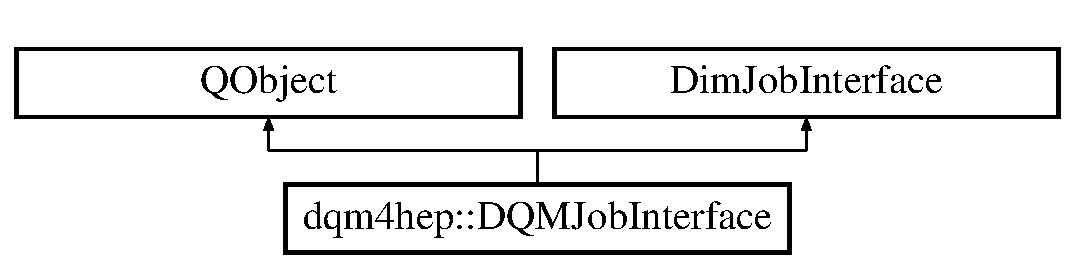
\includegraphics[height=2.000000cm]{classdqm4hep_1_1DQMJobInterface}
\end{center}
\end{figure}
\subsection*{Public Slots}
\begin{DoxyCompactItemize}
\item 
void {\bf start\+Update} (int n\+Seconds)
\begin{DoxyCompactList}\small\item\em Start update. \end{DoxyCompactList}\item 
void {\bf stop\+Update} ()
\begin{DoxyCompactList}\small\item\em Stop update. \end{DoxyCompactList}\end{DoxyCompactItemize}
\subsection*{Signals}
\begin{DoxyCompactItemize}
\item 
void {\bf status\+Received} (const Q\+String \&host\+Name)
\begin{DoxyCompactList}\small\item\em Signal emitted when job status are received. \end{DoxyCompactList}\end{DoxyCompactItemize}
\subsection*{Public Member Functions}
\begin{DoxyCompactItemize}
\item 
{\bf D\+Q\+M\+Job\+Interface} ()
\begin{DoxyCompactList}\small\item\em Constructor. \end{DoxyCompactList}\item 
virtual {\bf $\sim$\+D\+Q\+M\+Job\+Interface} ()
\begin{DoxyCompactList}\small\item\em Destructor. \end{DoxyCompactList}\item 
bool {\bf started} () const 
\begin{DoxyCompactList}\small\item\em Whether the automatic update mode has been started. \end{DoxyCompactList}\end{DoxyCompactItemize}
\subsection*{Private Member Functions}
\begin{DoxyCompactItemize}
\item 
void {\bf status\+Received} (const std\+::string \&host\+Name)
\begin{DoxyCompactList}\small\item\em Call back method when jobs status are received. \end{DoxyCompactList}\end{DoxyCompactItemize}
\subsection*{Private Attributes}
\begin{DoxyCompactItemize}
\item 
bool {\bf m\+\_\+started}
\end{DoxyCompactItemize}


\subsection{Detailed Description}
\doxyref{D\+Q\+M\+Job\+Interface}{p.}{classdqm4hep_1_1DQMJobInterface} class. 

Definition at line 43 of file D\+Q\+M\+Job\+Interface.\+h.



\subsection{Constructor \& Destructor Documentation}
\index{dqm4hep\+::\+D\+Q\+M\+Job\+Interface@{dqm4hep\+::\+D\+Q\+M\+Job\+Interface}!D\+Q\+M\+Job\+Interface@{D\+Q\+M\+Job\+Interface}}
\index{D\+Q\+M\+Job\+Interface@{D\+Q\+M\+Job\+Interface}!dqm4hep\+::\+D\+Q\+M\+Job\+Interface@{dqm4hep\+::\+D\+Q\+M\+Job\+Interface}}
\subsubsection[{D\+Q\+M\+Job\+Interface}]{\setlength{\rightskip}{0pt plus 5cm}dqm4hep\+::\+D\+Q\+M\+Job\+Interface\+::\+D\+Q\+M\+Job\+Interface (
\begin{DoxyParamCaption}
{}
\end{DoxyParamCaption}
)}\label{classdqm4hep_1_1DQMJobInterface_aade700478dee032ddfa1d8ad07c534fa}


Constructor. 



Definition at line 34 of file D\+Q\+M\+Job\+Interface.\+cc.


\begin{DoxyCode}
34                                  :
35     DimJobInterface(),
36     m_started(\textcolor{keyword}{false})
37 \{
38   \textcolor{comment}{/* nop */}
39 \}
\end{DoxyCode}
\index{dqm4hep\+::\+D\+Q\+M\+Job\+Interface@{dqm4hep\+::\+D\+Q\+M\+Job\+Interface}!````~D\+Q\+M\+Job\+Interface@{$\sim$\+D\+Q\+M\+Job\+Interface}}
\index{````~D\+Q\+M\+Job\+Interface@{$\sim$\+D\+Q\+M\+Job\+Interface}!dqm4hep\+::\+D\+Q\+M\+Job\+Interface@{dqm4hep\+::\+D\+Q\+M\+Job\+Interface}}
\subsubsection[{$\sim$\+D\+Q\+M\+Job\+Interface}]{\setlength{\rightskip}{0pt plus 5cm}dqm4hep\+::\+D\+Q\+M\+Job\+Interface\+::$\sim$\+D\+Q\+M\+Job\+Interface (
\begin{DoxyParamCaption}
{}
\end{DoxyParamCaption}
)\hspace{0.3cm}{\ttfamily [virtual]}}\label{classdqm4hep_1_1DQMJobInterface_a0753c68b3ca76ca2543ad312a64518cf}


Destructor. 



Definition at line 43 of file D\+Q\+M\+Job\+Interface.\+cc.


\begin{DoxyCode}
44 \{
45   \textcolor{comment}{/* nop */}
46 \}
\end{DoxyCode}


\subsection{Member Function Documentation}
\index{dqm4hep\+::\+D\+Q\+M\+Job\+Interface@{dqm4hep\+::\+D\+Q\+M\+Job\+Interface}!started@{started}}
\index{started@{started}!dqm4hep\+::\+D\+Q\+M\+Job\+Interface@{dqm4hep\+::\+D\+Q\+M\+Job\+Interface}}
\subsubsection[{started}]{\setlength{\rightskip}{0pt plus 5cm}bool dqm4hep\+::\+D\+Q\+M\+Job\+Interface\+::started (
\begin{DoxyParamCaption}
{}
\end{DoxyParamCaption}
) const}\label{classdqm4hep_1_1DQMJobInterface_acf2d6830a087e828e3335537452ae8b4}


Whether the automatic update mode has been started. 



Definition at line 50 of file D\+Q\+M\+Job\+Interface.\+cc.



References m\+\_\+started.



Referenced by dqm4hep\+::\+D\+Q\+M\+Job\+Interface\+Widget\+::handle\+Automatic\+Mode\+Button\+Clicked(), and dqm4hep\+::\+D\+Q\+M\+Job\+Interface\+Widget\+::handle\+Automatic\+Mode\+Value\+Changed().


\begin{DoxyCode}
51 \{
52   \textcolor{keywordflow}{return} m_started;
53 \}
\end{DoxyCode}
\index{dqm4hep\+::\+D\+Q\+M\+Job\+Interface@{dqm4hep\+::\+D\+Q\+M\+Job\+Interface}!start\+Update@{start\+Update}}
\index{start\+Update@{start\+Update}!dqm4hep\+::\+D\+Q\+M\+Job\+Interface@{dqm4hep\+::\+D\+Q\+M\+Job\+Interface}}
\subsubsection[{start\+Update}]{\setlength{\rightskip}{0pt plus 5cm}void dqm4hep\+::\+D\+Q\+M\+Job\+Interface\+::start\+Update (
\begin{DoxyParamCaption}
\item[{int}]{n\+Seconds}
\end{DoxyParamCaption}
)\hspace{0.3cm}{\ttfamily [slot]}}\label{classdqm4hep_1_1DQMJobInterface_a7b6f7b149ba51af3223760d0d9c52787}


Start update. 

Alias slot function for start\+Timer(n\+Seconds) 

Definition at line 57 of file D\+Q\+M\+Job\+Interface.\+cc.



References m\+\_\+started.



Referenced by dqm4hep\+::\+D\+Q\+M\+Job\+Interface\+Widget\+::handle\+Automatic\+Mode\+Button\+Clicked(), and dqm4hep\+::\+D\+Q\+M\+Job\+Interface\+Widget\+::handle\+Automatic\+Mode\+Value\+Changed().


\begin{DoxyCode}
58 \{
59   \textcolor{keywordflow}{if}(m_started)
60     DimJobInterface::stopTimer();
61 
62   DimJobInterface::startTimer(nSeconds);
63   m_started = \textcolor{keyword}{true};
64 \}
\end{DoxyCode}
\index{dqm4hep\+::\+D\+Q\+M\+Job\+Interface@{dqm4hep\+::\+D\+Q\+M\+Job\+Interface}!status\+Received@{status\+Received}}
\index{status\+Received@{status\+Received}!dqm4hep\+::\+D\+Q\+M\+Job\+Interface@{dqm4hep\+::\+D\+Q\+M\+Job\+Interface}}
\subsubsection[{status\+Received}]{\setlength{\rightskip}{0pt plus 5cm}void dqm4hep\+::\+D\+Q\+M\+Job\+Interface\+::status\+Received (
\begin{DoxyParamCaption}
\item[{const std\+::string \&}]{host\+Name}
\end{DoxyParamCaption}
)\hspace{0.3cm}{\ttfamily [private]}}\label{classdqm4hep_1_1DQMJobInterface_a5b6386494112b9210198b7d4b4146b1b}


Call back method when jobs status are received. 



Definition at line 78 of file D\+Q\+M\+Job\+Interface.\+cc.


\begin{DoxyCode}
79 \{
80   emit statusReceived(QString(hostName.c\_str()));
81 \}
\end{DoxyCode}
\index{dqm4hep\+::\+D\+Q\+M\+Job\+Interface@{dqm4hep\+::\+D\+Q\+M\+Job\+Interface}!status\+Received@{status\+Received}}
\index{status\+Received@{status\+Received}!dqm4hep\+::\+D\+Q\+M\+Job\+Interface@{dqm4hep\+::\+D\+Q\+M\+Job\+Interface}}
\subsubsection[{status\+Received}]{\setlength{\rightskip}{0pt plus 5cm}void dqm4hep\+::\+D\+Q\+M\+Job\+Interface\+::status\+Received (
\begin{DoxyParamCaption}
\item[{const Q\+String \&}]{host\+Name}
\end{DoxyParamCaption}
)\hspace{0.3cm}{\ttfamily [signal]}}\label{classdqm4hep_1_1DQMJobInterface_a9790fab51e895ab8798dd5441394a99e}


Signal emitted when job status are received. 

\index{dqm4hep\+::\+D\+Q\+M\+Job\+Interface@{dqm4hep\+::\+D\+Q\+M\+Job\+Interface}!stop\+Update@{stop\+Update}}
\index{stop\+Update@{stop\+Update}!dqm4hep\+::\+D\+Q\+M\+Job\+Interface@{dqm4hep\+::\+D\+Q\+M\+Job\+Interface}}
\subsubsection[{stop\+Update}]{\setlength{\rightskip}{0pt plus 5cm}void dqm4hep\+::\+D\+Q\+M\+Job\+Interface\+::stop\+Update (
\begin{DoxyParamCaption}
{}
\end{DoxyParamCaption}
)\hspace{0.3cm}{\ttfamily [slot]}}\label{classdqm4hep_1_1DQMJobInterface_a6e24685b7416c7f7af4295030bc995dc}


Stop update. 

Alias slot function for stop\+Timer() 

Definition at line 68 of file D\+Q\+M\+Job\+Interface.\+cc.



References m\+\_\+started.



Referenced by dqm4hep\+::\+D\+Q\+M\+Job\+Interface\+Widget\+::handle\+Automatic\+Mode\+Button\+Clicked(), and dqm4hep\+::\+D\+Q\+M\+Job\+Interface\+Widget\+::handle\+Automatic\+Mode\+Value\+Changed().


\begin{DoxyCode}
69 \{
70   \textcolor{keywordflow}{if}(m_started)
71     DimJobInterface::stopTimer();
72 
73   m_started = \textcolor{keyword}{false};
74 \}
\end{DoxyCode}


\subsection{Member Data Documentation}
\index{dqm4hep\+::\+D\+Q\+M\+Job\+Interface@{dqm4hep\+::\+D\+Q\+M\+Job\+Interface}!m\+\_\+started@{m\+\_\+started}}
\index{m\+\_\+started@{m\+\_\+started}!dqm4hep\+::\+D\+Q\+M\+Job\+Interface@{dqm4hep\+::\+D\+Q\+M\+Job\+Interface}}
\subsubsection[{m\+\_\+started}]{\setlength{\rightskip}{0pt plus 5cm}bool dqm4hep\+::\+D\+Q\+M\+Job\+Interface\+::m\+\_\+started\hspace{0.3cm}{\ttfamily [private]}}\label{classdqm4hep_1_1DQMJobInterface_a6b071eb9d7006e71f3b5bf0ead16ac0b}


Definition at line 83 of file D\+Q\+M\+Job\+Interface.\+h.



Referenced by started(), start\+Update(), and stop\+Update().



The documentation for this class was generated from the following files\+:\begin{DoxyCompactItemize}
\item 
{\bf D\+Q\+M\+Job\+Interface.\+h}\item 
{\bf D\+Q\+M\+Job\+Interface.\+cc}\end{DoxyCompactItemize}

\section{dqm4hep\+:\+:D\+Q\+M\+Job\+Interface\+Widget Class Reference}
\label{classdqm4hep_1_1DQMJobInterfaceWidget}\index{dqm4hep\+::\+D\+Q\+M\+Job\+Interface\+Widget@{dqm4hep\+::\+D\+Q\+M\+Job\+Interface\+Widget}}


\doxyref{D\+Q\+M\+Job\+Interface\+Widget}{p.}{classdqm4hep_1_1DQMJobInterfaceWidget} class.  




{\ttfamily \#include $<$D\+Q\+M\+Job\+Interface\+Widget.\+h$>$}

Inheritance diagram for dqm4hep\+:\+:D\+Q\+M\+Job\+Interface\+Widget\+:\begin{figure}[H]
\begin{center}
\leavevmode
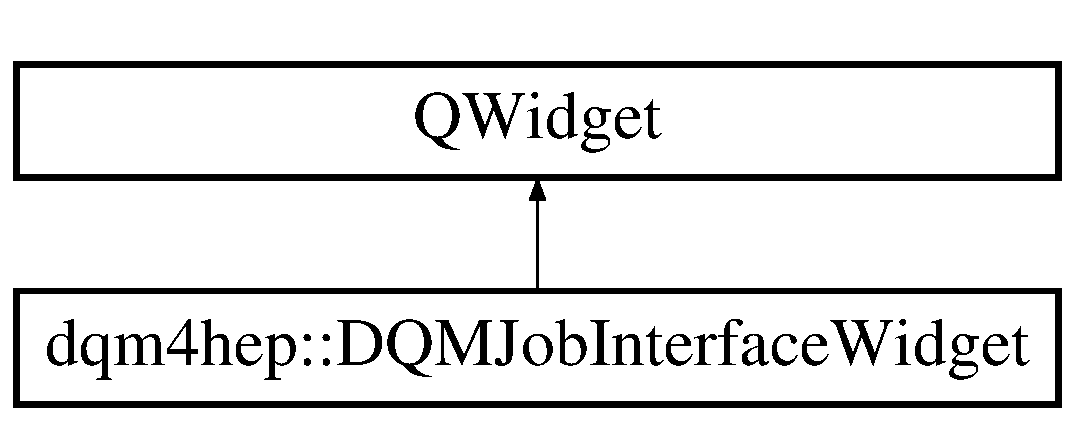
\includegraphics[height=2.000000cm]{classdqm4hep_1_1DQMJobInterfaceWidget}
\end{center}
\end{figure}
\subsection*{Public Types}
\begin{DoxyCompactItemize}
\item 
enum {\bf Item\+Type} \{ \\*
{\bf H\+O\+S\+T\+\_\+\+I\+T\+E\+M}, 
{\bf J\+O\+B\+\_\+\+I\+T\+E\+M}, 
{\bf J\+O\+B\+\_\+\+S\+T\+A\+T\+U\+S\+\_\+\+I\+T\+E\+M}, 
{\bf J\+O\+B\+\_\+\+P\+R\+O\+G\+R\+A\+M\+\_\+\+N\+A\+M\+E\+\_\+\+I\+T\+E\+M}, 
\\*
{\bf J\+O\+B\+\_\+\+P\+I\+D\+\_\+\+I\+T\+E\+M}, 
{\bf J\+O\+B\+\_\+\+E\+N\+V\+\_\+\+I\+T\+E\+M}, 
{\bf J\+O\+B\+\_\+\+A\+R\+G\+S\+\_\+\+I\+T\+E\+M}, 
{\bf V\+A\+R\+I\+A\+B\+L\+E\+\_\+\+I\+T\+E\+M}
 \}
\begin{DoxyCompactList}\small\item\em Item\+Type enum. \end{DoxyCompactList}\end{DoxyCompactItemize}
\subsection*{Public Slots}
\begin{DoxyCompactItemize}
\item 
void {\bf load\+Json\+File} (const std\+::string \&file\+Name)
\begin{DoxyCompactList}\small\item\em Load json file. \end{DoxyCompactList}\item 
void {\bf start\+Host\+Jobs} ()
\item 
void {\bf start\+All\+Jobs} ()
\item 
void {\bf start\+Selected\+Job} ()
\item 
void {\bf clear\+Host\+Jobs} ()
\item 
void {\bf clear\+All\+Jobs} ()
\item 
void {\bf kill\+Selected\+Job} ()
\item 
void {\bf restart\+Selected\+Job} ()
\item 
void {\bf restart\+All\+Jobs} ()
\item 
void {\bf update\+Job\+Status} ()
\end{DoxyCompactItemize}
\subsection*{Public Member Functions}
\begin{DoxyCompactItemize}
\item 
{\bf D\+Q\+M\+Job\+Interface\+Widget} (Q\+Widget $\ast$p\+Parent=N\+U\+L\+L)
\begin{DoxyCompactList}\small\item\em Constructor. \end{DoxyCompactList}\item 
{\bf $\sim$\+D\+Q\+M\+Job\+Interface\+Widget} ()
\begin{DoxyCompactList}\small\item\em Destructor. \end{DoxyCompactList}\item 
const std\+::string \& {\bf get\+Current\+Json\+File} () const 
\begin{DoxyCompactList}\small\item\em Get the current json file name. \end{DoxyCompactList}\item 
{\bf D\+Q\+M\+Job\+Interface} $\ast$ {\bf get\+Job\+Interface} () const 
\begin{DoxyCompactList}\small\item\em Get the job interface implementation. \end{DoxyCompactList}\end{DoxyCompactItemize}
\subsection*{Private Types}
\begin{DoxyCompactItemize}
\item 
enum {\bf Column\+Type} \{ {\bf N\+A\+M\+E}, 
{\bf P\+R\+O\+G\+\_\+\+N\+A\+M\+E}, 
{\bf P\+I\+D}, 
{\bf S\+T\+A\+T\+U\+S}
 \}
\end{DoxyCompactItemize}
\subsection*{Private Slots}
\begin{DoxyCompactItemize}
\item 
void {\bf load\+Json\+File} ()
\item 
void {\bf reload\+Json\+File} ()
\item 
void {\bf handle\+Automatic\+Mode\+Button\+Clicked} ()
\item 
void {\bf handle\+Automatic\+Mode\+Value\+Changed} (int value)
\item 
void {\bf update\+Status} (const Q\+String \&host\+Name)
\end{DoxyCompactItemize}
\subsection*{Private Member Functions}
\begin{DoxyCompactItemize}
\item 
void {\bf load\+Json} (const Json\+::\+Value \&root)
\item 
void {\bf update\+Status} (const Json\+::\+Value \&value)
\item 
void {\bf create\+Actions} ()
\item 
void {\bf create\+Menus} ()
\item 
void {\bf context\+Menu\+Event} (Q\+Context\+Menu\+Event $\ast$event)
\item 
bool {\bf job\+Control\+Exists} (const std\+::string \&host\+Name) const 
\item 
Q\+String\+List {\bf get\+Non\+Running\+Job\+Controls} () const 
\item 
void {\bf popup\+Missing\+Job\+Control} (const Q\+String \&host\+Name)
\item 
void {\bf popup\+Missing\+Job\+Controls} (const Q\+String\+List \&host\+Name)
\end{DoxyCompactItemize}
\subsection*{Private Attributes}
\begin{DoxyCompactItemize}
\item 
{\bf D\+Q\+M\+Job\+Interface} $\ast$ {\bf m\+\_\+p\+Job\+Iterface}
\item 
std\+::string {\bf m\+\_\+current\+Json\+File}
\item 
Q\+Push\+Button $\ast$ {\bf m\+\_\+p\+Automatic\+Mode\+Button}
\item 
Q\+Spin\+Box $\ast$ {\bf m\+\_\+p\+Update\+Period\+Spin\+Box}
\item 
Q\+Combo\+Box $\ast$ {\bf m\+\_\+p\+Kill\+Combo\+Box\+Widget}
\item 
Q\+Tree\+Widget $\ast$ {\bf m\+\_\+p\+Tree\+Widget}
\item 
Q\+Push\+Button $\ast$ {\bf m\+\_\+p\+Load\+File\+Button}
\item 
Q\+Push\+Button $\ast$ {\bf m\+\_\+p\+Reload\+File\+Button}
\item 
Q\+Push\+Button $\ast$ {\bf m\+\_\+p\+Start\+Host\+Jobs\+Button}
\item 
Q\+Push\+Button $\ast$ {\bf m\+\_\+p\+Clear\+Host\+Jobs\+Button}
\item 
Q\+Push\+Button $\ast$ {\bf m\+\_\+p\+Kill\+Job\+Button}
\item 
Q\+Push\+Button $\ast$ {\bf m\+\_\+p\+Restart\+Job\+Button}
\item 
Q\+Push\+Button $\ast$ {\bf m\+\_\+p\+Clear\+All\+Jobs\+Button}
\item 
Q\+Push\+Button $\ast$ {\bf m\+\_\+p\+Restart\+All\+Jobs\+Button}
\item 
Q\+Push\+Button $\ast$ {\bf m\+\_\+p\+Start\+All\+Jobs\+Button}
\item 
Q\+Push\+Button $\ast$ {\bf m\+\_\+p\+Update\+Button}
\item 
Q\+Menu\+Bar $\ast$ {\bf m\+\_\+p\+Menu\+Bar}
\item 
Q\+Menu $\ast$ {\bf m\+\_\+p\+Context\+Menu}
\item 
Q\+Menu $\ast$ {\bf m\+\_\+p\+File\+Menu}
\item 
Q\+Menu $\ast$ {\bf m\+\_\+p\+Help\+Menu}
\item 
Q\+Action $\ast$ {\bf m\+\_\+p\+Load\+File\+Action}
\item 
Q\+Action $\ast$ {\bf m\+\_\+p\+Reload\+File\+Action}
\item 
Q\+Action $\ast$ {\bf m\+\_\+p\+Start\+Host\+Jobs\+Action}
\item 
Q\+Action $\ast$ {\bf m\+\_\+p\+Clear\+Host\+Jobs\+Action}
\item 
Q\+Action $\ast$ {\bf m\+\_\+p\+Kill\+Job\+Action}
\item 
Q\+Action $\ast$ {\bf m\+\_\+p\+Start\+Job\+Action}
\item 
Q\+Action $\ast$ {\bf m\+\_\+p\+Restart\+Job\+Action}
\item 
Q\+Action $\ast$ {\bf m\+\_\+p\+Clear\+All\+Jobs\+Action}
\item 
Q\+Action $\ast$ {\bf m\+\_\+p\+Restart\+All\+Jobs\+Action}
\item 
Q\+Action $\ast$ {\bf m\+\_\+p\+Start\+All\+Jobs\+Action}
\item 
Q\+Action $\ast$ {\bf m\+\_\+p\+Update\+Action}
\end{DoxyCompactItemize}


\subsection{Detailed Description}
\doxyref{D\+Q\+M\+Job\+Interface\+Widget}{p.}{classdqm4hep_1_1DQMJobInterfaceWidget} class. 

Definition at line 54 of file D\+Q\+M\+Job\+Interface\+Widget.\+h.



\subsection{Member Enumeration Documentation}
\index{dqm4hep\+::\+D\+Q\+M\+Job\+Interface\+Widget@{dqm4hep\+::\+D\+Q\+M\+Job\+Interface\+Widget}!Column\+Type@{Column\+Type}}
\index{Column\+Type@{Column\+Type}!dqm4hep\+::\+D\+Q\+M\+Job\+Interface\+Widget@{dqm4hep\+::\+D\+Q\+M\+Job\+Interface\+Widget}}
\subsubsection[{Column\+Type}]{\setlength{\rightskip}{0pt plus 5cm}enum {\bf dqm4hep\+::\+D\+Q\+M\+Job\+Interface\+Widget\+::\+Column\+Type}\hspace{0.3cm}{\ttfamily [private]}}\label{classdqm4hep_1_1DQMJobInterfaceWidget_a86a0fe0a2a2ca209e94b2256af2d5ff1}
\begin{Desc}
\item[Enumerator]\par
\begin{description}
\index{N\+A\+M\+E@{N\+A\+M\+E}!dqm4hep\+::\+D\+Q\+M\+Job\+Interface\+Widget@{dqm4hep\+::\+D\+Q\+M\+Job\+Interface\+Widget}}\index{dqm4hep\+::\+D\+Q\+M\+Job\+Interface\+Widget@{dqm4hep\+::\+D\+Q\+M\+Job\+Interface\+Widget}!N\+A\+M\+E@{N\+A\+M\+E}}\item[{\em 
N\+A\+M\+E\label{classdqm4hep_1_1DQMJobInterfaceWidget_a86a0fe0a2a2ca209e94b2256af2d5ff1a7f5294cd1288d41eeecd53152b636ab6}
}]\index{P\+R\+O\+G\+\_\+\+N\+A\+M\+E@{P\+R\+O\+G\+\_\+\+N\+A\+M\+E}!dqm4hep\+::\+D\+Q\+M\+Job\+Interface\+Widget@{dqm4hep\+::\+D\+Q\+M\+Job\+Interface\+Widget}}\index{dqm4hep\+::\+D\+Q\+M\+Job\+Interface\+Widget@{dqm4hep\+::\+D\+Q\+M\+Job\+Interface\+Widget}!P\+R\+O\+G\+\_\+\+N\+A\+M\+E@{P\+R\+O\+G\+\_\+\+N\+A\+M\+E}}\item[{\em 
P\+R\+O\+G\+\_\+\+N\+A\+M\+E\label{classdqm4hep_1_1DQMJobInterfaceWidget_a86a0fe0a2a2ca209e94b2256af2d5ff1a3e17d3481bcbd80c73cb3003142c6b4e}
}]\index{P\+I\+D@{P\+I\+D}!dqm4hep\+::\+D\+Q\+M\+Job\+Interface\+Widget@{dqm4hep\+::\+D\+Q\+M\+Job\+Interface\+Widget}}\index{dqm4hep\+::\+D\+Q\+M\+Job\+Interface\+Widget@{dqm4hep\+::\+D\+Q\+M\+Job\+Interface\+Widget}!P\+I\+D@{P\+I\+D}}\item[{\em 
P\+I\+D\label{classdqm4hep_1_1DQMJobInterfaceWidget_a86a0fe0a2a2ca209e94b2256af2d5ff1a1ece3718b091903763b8f6e100c2cfa8}
}]\index{S\+T\+A\+T\+U\+S@{S\+T\+A\+T\+U\+S}!dqm4hep\+::\+D\+Q\+M\+Job\+Interface\+Widget@{dqm4hep\+::\+D\+Q\+M\+Job\+Interface\+Widget}}\index{dqm4hep\+::\+D\+Q\+M\+Job\+Interface\+Widget@{dqm4hep\+::\+D\+Q\+M\+Job\+Interface\+Widget}!S\+T\+A\+T\+U\+S@{S\+T\+A\+T\+U\+S}}\item[{\em 
S\+T\+A\+T\+U\+S\label{classdqm4hep_1_1DQMJobInterfaceWidget_a86a0fe0a2a2ca209e94b2256af2d5ff1a1d8713ed12aadb4b006fd5f9d172afd6}
}]\end{description}
\end{Desc}


Definition at line 153 of file D\+Q\+M\+Job\+Interface\+Widget.\+h.


\begin{DoxyCode}
154     \{
155         NAME,
156         PROG_NAME,
157         PID,
158         STATUS
159     \};
\end{DoxyCode}
\index{dqm4hep\+::\+D\+Q\+M\+Job\+Interface\+Widget@{dqm4hep\+::\+D\+Q\+M\+Job\+Interface\+Widget}!Item\+Type@{Item\+Type}}
\index{Item\+Type@{Item\+Type}!dqm4hep\+::\+D\+Q\+M\+Job\+Interface\+Widget@{dqm4hep\+::\+D\+Q\+M\+Job\+Interface\+Widget}}
\subsubsection[{Item\+Type}]{\setlength{\rightskip}{0pt plus 5cm}enum {\bf dqm4hep\+::\+D\+Q\+M\+Job\+Interface\+Widget\+::\+Item\+Type}}\label{classdqm4hep_1_1DQMJobInterfaceWidget_ace003d0a512942a0e3b5fe40171e06e3}


Item\+Type enum. 

\begin{Desc}
\item[Enumerator]\par
\begin{description}
\index{H\+O\+S\+T\+\_\+\+I\+T\+E\+M@{H\+O\+S\+T\+\_\+\+I\+T\+E\+M}!dqm4hep\+::\+D\+Q\+M\+Job\+Interface\+Widget@{dqm4hep\+::\+D\+Q\+M\+Job\+Interface\+Widget}}\index{dqm4hep\+::\+D\+Q\+M\+Job\+Interface\+Widget@{dqm4hep\+::\+D\+Q\+M\+Job\+Interface\+Widget}!H\+O\+S\+T\+\_\+\+I\+T\+E\+M@{H\+O\+S\+T\+\_\+\+I\+T\+E\+M}}\item[{\em 
H\+O\+S\+T\+\_\+\+I\+T\+E\+M\label{classdqm4hep_1_1DQMJobInterfaceWidget_ace003d0a512942a0e3b5fe40171e06e3a2650195c4cbf8bfdbcc5e49b2bef4654}
}]\index{J\+O\+B\+\_\+\+I\+T\+E\+M@{J\+O\+B\+\_\+\+I\+T\+E\+M}!dqm4hep\+::\+D\+Q\+M\+Job\+Interface\+Widget@{dqm4hep\+::\+D\+Q\+M\+Job\+Interface\+Widget}}\index{dqm4hep\+::\+D\+Q\+M\+Job\+Interface\+Widget@{dqm4hep\+::\+D\+Q\+M\+Job\+Interface\+Widget}!J\+O\+B\+\_\+\+I\+T\+E\+M@{J\+O\+B\+\_\+\+I\+T\+E\+M}}\item[{\em 
J\+O\+B\+\_\+\+I\+T\+E\+M\label{classdqm4hep_1_1DQMJobInterfaceWidget_ace003d0a512942a0e3b5fe40171e06e3a8ec8a7251715ed9b27eeed7ff583bd54}
}]\index{J\+O\+B\+\_\+\+S\+T\+A\+T\+U\+S\+\_\+\+I\+T\+E\+M@{J\+O\+B\+\_\+\+S\+T\+A\+T\+U\+S\+\_\+\+I\+T\+E\+M}!dqm4hep\+::\+D\+Q\+M\+Job\+Interface\+Widget@{dqm4hep\+::\+D\+Q\+M\+Job\+Interface\+Widget}}\index{dqm4hep\+::\+D\+Q\+M\+Job\+Interface\+Widget@{dqm4hep\+::\+D\+Q\+M\+Job\+Interface\+Widget}!J\+O\+B\+\_\+\+S\+T\+A\+T\+U\+S\+\_\+\+I\+T\+E\+M@{J\+O\+B\+\_\+\+S\+T\+A\+T\+U\+S\+\_\+\+I\+T\+E\+M}}\item[{\em 
J\+O\+B\+\_\+\+S\+T\+A\+T\+U\+S\+\_\+\+I\+T\+E\+M\label{classdqm4hep_1_1DQMJobInterfaceWidget_ace003d0a512942a0e3b5fe40171e06e3ac0c331c52cf71173cca29003488ccf01}
}]\index{J\+O\+B\+\_\+\+P\+R\+O\+G\+R\+A\+M\+\_\+\+N\+A\+M\+E\+\_\+\+I\+T\+E\+M@{J\+O\+B\+\_\+\+P\+R\+O\+G\+R\+A\+M\+\_\+\+N\+A\+M\+E\+\_\+\+I\+T\+E\+M}!dqm4hep\+::\+D\+Q\+M\+Job\+Interface\+Widget@{dqm4hep\+::\+D\+Q\+M\+Job\+Interface\+Widget}}\index{dqm4hep\+::\+D\+Q\+M\+Job\+Interface\+Widget@{dqm4hep\+::\+D\+Q\+M\+Job\+Interface\+Widget}!J\+O\+B\+\_\+\+P\+R\+O\+G\+R\+A\+M\+\_\+\+N\+A\+M\+E\+\_\+\+I\+T\+E\+M@{J\+O\+B\+\_\+\+P\+R\+O\+G\+R\+A\+M\+\_\+\+N\+A\+M\+E\+\_\+\+I\+T\+E\+M}}\item[{\em 
J\+O\+B\+\_\+\+P\+R\+O\+G\+R\+A\+M\+\_\+\+N\+A\+M\+E\+\_\+\+I\+T\+E\+M\label{classdqm4hep_1_1DQMJobInterfaceWidget_ace003d0a512942a0e3b5fe40171e06e3a0d4f3db9246c7c6c4bb6f65d1e01cb0a}
}]\index{J\+O\+B\+\_\+\+P\+I\+D\+\_\+\+I\+T\+E\+M@{J\+O\+B\+\_\+\+P\+I\+D\+\_\+\+I\+T\+E\+M}!dqm4hep\+::\+D\+Q\+M\+Job\+Interface\+Widget@{dqm4hep\+::\+D\+Q\+M\+Job\+Interface\+Widget}}\index{dqm4hep\+::\+D\+Q\+M\+Job\+Interface\+Widget@{dqm4hep\+::\+D\+Q\+M\+Job\+Interface\+Widget}!J\+O\+B\+\_\+\+P\+I\+D\+\_\+\+I\+T\+E\+M@{J\+O\+B\+\_\+\+P\+I\+D\+\_\+\+I\+T\+E\+M}}\item[{\em 
J\+O\+B\+\_\+\+P\+I\+D\+\_\+\+I\+T\+E\+M\label{classdqm4hep_1_1DQMJobInterfaceWidget_ace003d0a512942a0e3b5fe40171e06e3a57c6c93c9378ab99e3e2ebbb29a69449}
}]\index{J\+O\+B\+\_\+\+E\+N\+V\+\_\+\+I\+T\+E\+M@{J\+O\+B\+\_\+\+E\+N\+V\+\_\+\+I\+T\+E\+M}!dqm4hep\+::\+D\+Q\+M\+Job\+Interface\+Widget@{dqm4hep\+::\+D\+Q\+M\+Job\+Interface\+Widget}}\index{dqm4hep\+::\+D\+Q\+M\+Job\+Interface\+Widget@{dqm4hep\+::\+D\+Q\+M\+Job\+Interface\+Widget}!J\+O\+B\+\_\+\+E\+N\+V\+\_\+\+I\+T\+E\+M@{J\+O\+B\+\_\+\+E\+N\+V\+\_\+\+I\+T\+E\+M}}\item[{\em 
J\+O\+B\+\_\+\+E\+N\+V\+\_\+\+I\+T\+E\+M\label{classdqm4hep_1_1DQMJobInterfaceWidget_ace003d0a512942a0e3b5fe40171e06e3a4fd7b3628d20f42f372121d1a309d6ab}
}]\index{J\+O\+B\+\_\+\+A\+R\+G\+S\+\_\+\+I\+T\+E\+M@{J\+O\+B\+\_\+\+A\+R\+G\+S\+\_\+\+I\+T\+E\+M}!dqm4hep\+::\+D\+Q\+M\+Job\+Interface\+Widget@{dqm4hep\+::\+D\+Q\+M\+Job\+Interface\+Widget}}\index{dqm4hep\+::\+D\+Q\+M\+Job\+Interface\+Widget@{dqm4hep\+::\+D\+Q\+M\+Job\+Interface\+Widget}!J\+O\+B\+\_\+\+A\+R\+G\+S\+\_\+\+I\+T\+E\+M@{J\+O\+B\+\_\+\+A\+R\+G\+S\+\_\+\+I\+T\+E\+M}}\item[{\em 
J\+O\+B\+\_\+\+A\+R\+G\+S\+\_\+\+I\+T\+E\+M\label{classdqm4hep_1_1DQMJobInterfaceWidget_ace003d0a512942a0e3b5fe40171e06e3a39a43252e7fd38be5e6dfe520848d587}
}]\index{V\+A\+R\+I\+A\+B\+L\+E\+\_\+\+I\+T\+E\+M@{V\+A\+R\+I\+A\+B\+L\+E\+\_\+\+I\+T\+E\+M}!dqm4hep\+::\+D\+Q\+M\+Job\+Interface\+Widget@{dqm4hep\+::\+D\+Q\+M\+Job\+Interface\+Widget}}\index{dqm4hep\+::\+D\+Q\+M\+Job\+Interface\+Widget@{dqm4hep\+::\+D\+Q\+M\+Job\+Interface\+Widget}!V\+A\+R\+I\+A\+B\+L\+E\+\_\+\+I\+T\+E\+M@{V\+A\+R\+I\+A\+B\+L\+E\+\_\+\+I\+T\+E\+M}}\item[{\em 
V\+A\+R\+I\+A\+B\+L\+E\+\_\+\+I\+T\+E\+M\label{classdqm4hep_1_1DQMJobInterfaceWidget_ace003d0a512942a0e3b5fe40171e06e3a1049c14bfa7c2c278e9221eab2df45ba}
}]\end{description}
\end{Desc}


Definition at line 61 of file D\+Q\+M\+Job\+Interface\+Widget.\+h.


\begin{DoxyCode}
62     \{
63         HOST_ITEM,
64         JOB_ITEM,
65         JOB_STATUS_ITEM,
66         JOB_PROGRAM_NAME_ITEM,
67         JOB_PID_ITEM,
68         JOB_ENV_ITEM,
69         JOB_ARGS_ITEM,
70         VARIABLE_ITEM
71     \};
\end{DoxyCode}


\subsection{Constructor \& Destructor Documentation}
\index{dqm4hep\+::\+D\+Q\+M\+Job\+Interface\+Widget@{dqm4hep\+::\+D\+Q\+M\+Job\+Interface\+Widget}!D\+Q\+M\+Job\+Interface\+Widget@{D\+Q\+M\+Job\+Interface\+Widget}}
\index{D\+Q\+M\+Job\+Interface\+Widget@{D\+Q\+M\+Job\+Interface\+Widget}!dqm4hep\+::\+D\+Q\+M\+Job\+Interface\+Widget@{dqm4hep\+::\+D\+Q\+M\+Job\+Interface\+Widget}}
\subsubsection[{D\+Q\+M\+Job\+Interface\+Widget}]{\setlength{\rightskip}{0pt plus 5cm}dqm4hep\+::\+D\+Q\+M\+Job\+Interface\+Widget\+::\+D\+Q\+M\+Job\+Interface\+Widget (
\begin{DoxyParamCaption}
\item[{Q\+Widget $\ast$}]{p\+Parent = {\ttfamily NULL}}
\end{DoxyParamCaption}
)}\label{classdqm4hep_1_1DQMJobInterfaceWidget_a2e5cff5d390acd242368ea3825798653}


Constructor. 



Definition at line 55 of file D\+Q\+M\+Job\+Interface\+Widget.\+cc.



References create\+Actions(), create\+Menus(), handle\+Automatic\+Mode\+Button\+Clicked(), handle\+Automatic\+Mode\+Value\+Changed(), load\+Json\+File(), m\+\_\+p\+Automatic\+Mode\+Button, m\+\_\+p\+Job\+Iterface, m\+\_\+p\+Kill\+Combo\+Box\+Widget, m\+\_\+p\+Load\+File\+Button, m\+\_\+p\+Reload\+File\+Button, m\+\_\+p\+Tree\+Widget, m\+\_\+p\+Update\+Button, m\+\_\+p\+Update\+Period\+Spin\+Box, reload\+Json\+File(), update\+Job\+Status(), and update\+Status().


\begin{DoxyCode}
55                                                             :
56     QWidget(pParent),
57     m_pAutomaticModeButton(0)
58 \{
59     m_pJobIterface = \textcolor{keyword}{new} DQMJobInterface();
60 
61     QLayout *pMainLayout = \textcolor{keyword}{new} QVBoxLayout();
62     setLayout(pMainLayout);
63 
64     QHBoxLayout *pComboBoxLayout = \textcolor{keyword}{new} QHBoxLayout();
65 
66     QGroupBox *pComboBoxGroupBox = \textcolor{keyword}{new} QGroupBox();
67     pMainLayout->addWidget(pComboBoxGroupBox);
68 
69     m_pAutomaticModeButton = \textcolor{keyword}{new} QPushButton(\textcolor{stringliteral}{"Start"});
70   pComboBoxLayout->addWidget(m_pAutomaticModeButton);
71 
72   QLabel *pUpdatePeriodLabel = \textcolor{keyword}{new} QLabel(\textcolor{stringliteral}{"Update period (secs) : "});
73   pComboBoxLayout->addWidget(pUpdatePeriodLabel);
74 
75   m_pUpdatePeriodSpinBox = \textcolor{keyword}{new} QSpinBox();
76   m_pUpdatePeriodSpinBox->setValue(5);
77   pComboBoxLayout->addWidget(m_pUpdatePeriodSpinBox);
78 
79   connect(m_pAutomaticModeButton, SIGNAL(clicked()), \textcolor{keyword}{this}, SLOT(
      handleAutomaticModeButtonClicked()));
80   connect(m_pUpdatePeriodSpinBox, SIGNAL(valueChanged(\textcolor{keywordtype}{int})), \textcolor{keyword}{this}, SLOT(
      handleAutomaticModeValueChanged(\textcolor{keywordtype}{int})));
81   connect(m_pJobIterface, SIGNAL(statusReceived(\textcolor{keyword}{const} QString &)), \textcolor{keyword}{this}, SLOT(
      updateStatus(\textcolor{keyword}{const} QString &)));
82 
83     QSpacerItem *p\_HSpacer = \textcolor{keyword}{new} QSpacerItem(1, 0, QSizePolicy::Expanding, QSizePolicy::Minimum);
84     pComboBoxLayout->addSpacerItem(p\_HSpacer);
85 
86     QLabel *pKillComboBoxCaption = \textcolor{keyword}{new} QLabel(\textcolor{stringliteral}{"Set Kill Method"});
87     pComboBoxLayout->addWidget(pKillComboBoxCaption);
88 
89     m_pKillComboBoxWidget = \textcolor{keyword}{new} QComboBox();
90     m_pKillComboBoxWidget->addItem(\textcolor{stringliteral}{"HUP (Hang Up): 1"}, 1);
91     m_pKillComboBoxWidget->addItem(\textcolor{stringliteral}{"INT (Interrupt): 2"}, 2);
92     m_pKillComboBoxWidget->addItem(\textcolor{stringliteral}{"QUIT (Quit): 3"}, 3);
93     m_pKillComboBoxWidget->addItem(\textcolor{stringliteral}{"ABRT (Abort): 6"}, 6);
94     m_pKillComboBoxWidget->addItem(\textcolor{stringliteral}{"KILL (Non-ignorable kill): 9"}, 9);
95     m_pKillComboBoxWidget->addItem(\textcolor{stringliteral}{"ALRM (Alarm Clock): 14"}, 14);
96     m_pKillComboBoxWidget->addItem(\textcolor{stringliteral}{"TERM (Software Term Signal): 15"}, 15);
97     m_pKillComboBoxWidget->setCurrentIndex(1); \textcolor{comment}{// Default: Interrupt = kill -2}
98 
99     pComboBoxLayout->addWidget(m_pKillComboBoxWidget);
100     pComboBoxGroupBox->setLayout(pComboBoxLayout);
101 
102     m_pTreeWidget = \textcolor{keyword}{new} QTreeWidget();
103     pMainLayout->addWidget(m_pTreeWidget);
104 
105     m_pTreeWidget->setColumnCount(4);
106     m_pTreeWidget->setHeaderLabels(QStringList() << \textcolor{stringliteral}{"Job Control"} << \textcolor{stringliteral}{"Program Name"} << \textcolor{stringliteral}{"PID"} << \textcolor{stringliteral}{"Status"});
107 
108     \textcolor{comment}{// Create Buttons}
109     QWidget *pButtonWidget = \textcolor{keyword}{new} QWidget();
110     pMainLayout->addWidget(pButtonWidget);
111 
112     QHBoxLayout *pButtonHLayout = \textcolor{keyword}{new} QHBoxLayout();
113     pButtonWidget->setLayout(pButtonHLayout);
114 
115     m_pLoadFileButton = \textcolor{keyword}{new} QPushButton(\textcolor{stringliteral}{"Load file"});
116     pButtonHLayout->addWidget(m_pLoadFileButton);
117     connect(m_pLoadFileButton, SIGNAL(clicked()), \textcolor{keyword}{this}, SLOT(loadJsonFile()));
118 
119     m_pReloadFileButton = \textcolor{keyword}{new} QPushButton(\textcolor{stringliteral}{"Reload file"});
120     pButtonHLayout->addWidget(m_pReloadFileButton);
121     connect(m_pReloadFileButton, SIGNAL(clicked()), \textcolor{keyword}{this}, SLOT(reloadJsonFile()));
122 
123     QSpacerItem *p\_HButtonSpacer = \textcolor{keyword}{new} QSpacerItem(1, 0, QSizePolicy::Expanding, QSizePolicy::Minimum);
124     pButtonHLayout->addSpacerItem(p\_HButtonSpacer);
125 
126     m_pUpdateButton = \textcolor{keyword}{new} QPushButton(\textcolor{stringliteral}{"Update"});
127     pButtonHLayout->addWidget(m_pUpdateButton);
128     connect(m_pUpdateButton, SIGNAL(clicked()), \textcolor{keyword}{this}, SLOT(updateJobStatus()));
129 
130     \textcolor{comment}{// Create Menus / Menus Entries}
131     createActions();
132     createMenus();
133 \}
\end{DoxyCode}
\index{dqm4hep\+::\+D\+Q\+M\+Job\+Interface\+Widget@{dqm4hep\+::\+D\+Q\+M\+Job\+Interface\+Widget}!````~D\+Q\+M\+Job\+Interface\+Widget@{$\sim$\+D\+Q\+M\+Job\+Interface\+Widget}}
\index{````~D\+Q\+M\+Job\+Interface\+Widget@{$\sim$\+D\+Q\+M\+Job\+Interface\+Widget}!dqm4hep\+::\+D\+Q\+M\+Job\+Interface\+Widget@{dqm4hep\+::\+D\+Q\+M\+Job\+Interface\+Widget}}
\subsubsection[{$\sim$\+D\+Q\+M\+Job\+Interface\+Widget}]{\setlength{\rightskip}{0pt plus 5cm}dqm4hep\+::\+D\+Q\+M\+Job\+Interface\+Widget\+::$\sim$\+D\+Q\+M\+Job\+Interface\+Widget (
\begin{DoxyParamCaption}
{}
\end{DoxyParamCaption}
)}\label{classdqm4hep_1_1DQMJobInterfaceWidget_afad2e49d4714b276206dadedfa7d4579}


Destructor. 



Definition at line 137 of file D\+Q\+M\+Job\+Interface\+Widget.\+cc.



References m\+\_\+p\+Job\+Iterface.


\begin{DoxyCode}
138 \{
139     \textcolor{keyword}{delete} m_pJobIterface;
140 \}
\end{DoxyCode}


\subsection{Member Function Documentation}
\index{dqm4hep\+::\+D\+Q\+M\+Job\+Interface\+Widget@{dqm4hep\+::\+D\+Q\+M\+Job\+Interface\+Widget}!clear\+All\+Jobs@{clear\+All\+Jobs}}
\index{clear\+All\+Jobs@{clear\+All\+Jobs}!dqm4hep\+::\+D\+Q\+M\+Job\+Interface\+Widget@{dqm4hep\+::\+D\+Q\+M\+Job\+Interface\+Widget}}
\subsubsection[{clear\+All\+Jobs}]{\setlength{\rightskip}{0pt plus 5cm}void dqm4hep\+::\+D\+Q\+M\+Job\+Interface\+Widget\+::clear\+All\+Jobs (
\begin{DoxyParamCaption}
{}
\end{DoxyParamCaption}
)\hspace{0.3cm}{\ttfamily [slot]}}\label{classdqm4hep_1_1DQMJobInterfaceWidget_a0fd8c5d0b4589a0ac88fd89e6b74ed0b}


Definition at line 429 of file D\+Q\+M\+Job\+Interface\+Widget.\+cc.



References get\+Non\+Running\+Job\+Controls(), m\+\_\+p\+Job\+Iterface, and popup\+Missing\+Job\+Controls().



Referenced by create\+Actions(), and load\+Json\+File().


\begin{DoxyCode}
430 \{
431     QStringList nonRunningJobControls = getNonRunningJobControls();
432 
433     \textcolor{keywordflow}{if}(!nonRunningJobControls.isEmpty())
434       popupMissingJobControls(nonRunningJobControls);
435 
436     m_pJobIterface->clearAllJobs();
437 \}
\end{DoxyCode}
\index{dqm4hep\+::\+D\+Q\+M\+Job\+Interface\+Widget@{dqm4hep\+::\+D\+Q\+M\+Job\+Interface\+Widget}!clear\+Host\+Jobs@{clear\+Host\+Jobs}}
\index{clear\+Host\+Jobs@{clear\+Host\+Jobs}!dqm4hep\+::\+D\+Q\+M\+Job\+Interface\+Widget@{dqm4hep\+::\+D\+Q\+M\+Job\+Interface\+Widget}}
\subsubsection[{clear\+Host\+Jobs}]{\setlength{\rightskip}{0pt plus 5cm}void dqm4hep\+::\+D\+Q\+M\+Job\+Interface\+Widget\+::clear\+Host\+Jobs (
\begin{DoxyParamCaption}
{}
\end{DoxyParamCaption}
)\hspace{0.3cm}{\ttfamily [slot]}}\label{classdqm4hep_1_1DQMJobInterfaceWidget_ac6c4551a458ba67d8747157d746519fb}


Definition at line 406 of file D\+Q\+M\+Job\+Interface\+Widget.\+cc.



References H\+O\+S\+T\+\_\+\+I\+T\+E\+M, job\+Control\+Exists(), m\+\_\+p\+Job\+Iterface, m\+\_\+p\+Tree\+Widget, N\+A\+M\+E, and popup\+Missing\+Job\+Control().



Referenced by create\+Actions().


\begin{DoxyCode}
407 \{
408     QTreeWidgetItem* pSelectedItem = m_pTreeWidget->currentItem();
409 
410     \textcolor{keywordflow}{if}(!pSelectedItem)
411         \textcolor{keywordflow}{return};
412 
413     \textcolor{keywordflow}{if}(pSelectedItem->data(0, Qt::UserRole).value<\textcolor{keywordtype}{int}>() != HOST_ITEM)
414         \textcolor{keywordflow}{return};
415 
416     QString hostName = pSelectedItem->text(NAME);
417 
418     \textcolor{keywordflow}{if}(!this->jobControlExists(hostName.toStdString()))
419     \{
420       popupMissingJobControl(hostName);
421       \textcolor{keywordflow}{return};
422     \}
423 
424     m_pJobIterface->clearHostJobs(hostName.toStdString());
425 \}
\end{DoxyCode}
\index{dqm4hep\+::\+D\+Q\+M\+Job\+Interface\+Widget@{dqm4hep\+::\+D\+Q\+M\+Job\+Interface\+Widget}!context\+Menu\+Event@{context\+Menu\+Event}}
\index{context\+Menu\+Event@{context\+Menu\+Event}!dqm4hep\+::\+D\+Q\+M\+Job\+Interface\+Widget@{dqm4hep\+::\+D\+Q\+M\+Job\+Interface\+Widget}}
\subsubsection[{context\+Menu\+Event}]{\setlength{\rightskip}{0pt plus 5cm}void dqm4hep\+::\+D\+Q\+M\+Job\+Interface\+Widget\+::context\+Menu\+Event (
\begin{DoxyParamCaption}
\item[{Q\+Context\+Menu\+Event $\ast$}]{event}
\end{DoxyParamCaption}
)\hspace{0.3cm}{\ttfamily [private]}}\label{classdqm4hep_1_1DQMJobInterfaceWidget_a0ff806c4f774b5f3832c6fb815e73210}


Definition at line 206 of file D\+Q\+M\+Job\+Interface\+Widget.\+cc.



References H\+O\+S\+T\+\_\+\+I\+T\+E\+M, J\+O\+B\+\_\+\+I\+T\+E\+M, m\+\_\+p\+Clear\+All\+Jobs\+Action, m\+\_\+p\+Clear\+Host\+Jobs\+Action, m\+\_\+p\+Context\+Menu, m\+\_\+p\+Kill\+Job\+Action, m\+\_\+p\+Restart\+All\+Jobs\+Action, m\+\_\+p\+Restart\+Job\+Action, m\+\_\+p\+Start\+All\+Jobs\+Action, m\+\_\+p\+Start\+Host\+Jobs\+Action, m\+\_\+p\+Start\+Job\+Action, m\+\_\+p\+Tree\+Widget, m\+\_\+p\+Update\+Action, P\+I\+D, and S\+T\+A\+T\+U\+S.


\begin{DoxyCode}
207 \{
208     m_pContextMenu = \textcolor{keyword}{new} QMenu();
209     m_pContextMenu->addAction(m_pStartHostJobsAction);
210     m_pContextMenu->addAction(m_pClearHostJobsAction);
211 
212     m_pContextMenu->addSeparator();
213     m_pContextMenu->addAction(m_pKillJobAction);
214     m_pContextMenu->addAction(m_pRestartJobAction);
215     m_pContextMenu->addAction(m_pStartJobAction);
216 
217     m_pContextMenu->addSeparator();
218     m_pContextMenu->addAction(m_pClearAllJobsAction);
219     m_pContextMenu->addAction(m_pRestartAllJobsAction);
220     m_pContextMenu->addAction(m_pStartAllJobsAction);
221 
222     m_pContextMenu->addSeparator();
223     m_pContextMenu->addAction(m_pUpdateAction);
224 
225     m_pStartHostJobsAction->setEnabled(\textcolor{keyword}{false});
226     m_pClearHostJobsAction->setEnabled(\textcolor{keyword}{false});
227     m_pKillJobAction->setEnabled(\textcolor{keyword}{false});
228     m_pRestartJobAction->setEnabled(\textcolor{keyword}{false});
229     m_pStartJobAction->setEnabled(\textcolor{keyword}{false});
230 
231     \textcolor{comment}{// Activate items as needed}
232     QTreeWidgetItem* pCurrentItem = m_pTreeWidget->currentItem();
233 
234     \textcolor{keywordflow}{if} (NULL == pCurrentItem)
235     \{
236         m_pContextMenu->exec(event->globalPos());
237         \textcolor{keywordflow}{return};
238     \}
239 
240     \textcolor{keywordflow}{if}(pCurrentItem->data(0, Qt::UserRole).value<\textcolor{keywordtype}{int}>() == HOST_ITEM)
241     \{
242         m_pStartHostJobsAction->setEnabled(\textcolor{keyword}{true});
243         m_pClearHostJobsAction->setEnabled(\textcolor{keyword}{true});
244     \}
245     \textcolor{keywordflow}{else} \textcolor{keywordflow}{if}(pCurrentItem->data(0, Qt::UserRole).value<\textcolor{keywordtype}{int}>() == JOB_ITEM)
246     \{
247         QString status = pCurrentItem->text(STATUS).at(0);
248 
249         \textcolor{keywordflow}{if} (status.isEmpty())
250             \textcolor{keywordflow}{return};
251 
252         \textcolor{keywordflow}{if} ( status == \textcolor{stringliteral}{"D"} || status == \textcolor{stringliteral}{"X"}) \textcolor{comment}{//Dead}
253         \{
254             \textcolor{keywordflow}{if} (pCurrentItem->text(PID).toInt())
255                 m_pRestartJobAction->setEnabled(\textcolor{keyword}{true});
256             \textcolor{keywordflow}{else}
257                 m_pStartJobAction->setEnabled(\textcolor{keyword}{true});
258         \}
259 
260         \textcolor{keywordflow}{else} \textcolor{keywordflow}{if} ( status != \textcolor{stringliteral}{"Z"} && \textcolor{comment}{// Zombie}
261                   status != \textcolor{stringliteral}{"T"}     \textcolor{comment}{// Traced or Stopped}
262                   )
263         \{
264             m_pKillJobAction->setEnabled(\textcolor{keyword}{true});
265             m_pRestartJobAction->setEnabled(\textcolor{keyword}{true});
266         \}
267         \textcolor{keywordflow}{else}
268         \{
269             m_pStartJobAction->setEnabled(\textcolor{keyword}{true});
270         \}
271     \}
272 
273     m_pContextMenu->exec(event->globalPos());
274 \}
\end{DoxyCode}
\index{dqm4hep\+::\+D\+Q\+M\+Job\+Interface\+Widget@{dqm4hep\+::\+D\+Q\+M\+Job\+Interface\+Widget}!create\+Actions@{create\+Actions}}
\index{create\+Actions@{create\+Actions}!dqm4hep\+::\+D\+Q\+M\+Job\+Interface\+Widget@{dqm4hep\+::\+D\+Q\+M\+Job\+Interface\+Widget}}
\subsubsection[{create\+Actions}]{\setlength{\rightskip}{0pt plus 5cm}void dqm4hep\+::\+D\+Q\+M\+Job\+Interface\+Widget\+::create\+Actions (
\begin{DoxyParamCaption}
{}
\end{DoxyParamCaption}
)\hspace{0.3cm}{\ttfamily [private]}}\label{classdqm4hep_1_1DQMJobInterfaceWidget_a4fb7afdbf89119d495ff8be57874306c}


Definition at line 158 of file D\+Q\+M\+Job\+Interface\+Widget.\+cc.



References clear\+All\+Jobs(), clear\+Host\+Jobs(), kill\+Selected\+Job(), load\+Json\+File(), m\+\_\+p\+Clear\+All\+Jobs\+Action, m\+\_\+p\+Clear\+Host\+Jobs\+Action, m\+\_\+p\+Kill\+Job\+Action, m\+\_\+p\+Load\+File\+Action, m\+\_\+p\+Reload\+File\+Action, m\+\_\+p\+Restart\+All\+Jobs\+Action, m\+\_\+p\+Restart\+Job\+Action, m\+\_\+p\+Start\+All\+Jobs\+Action, m\+\_\+p\+Start\+Host\+Jobs\+Action, m\+\_\+p\+Start\+Job\+Action, m\+\_\+p\+Update\+Action, reload\+Json\+File(), restart\+All\+Jobs(), restart\+Selected\+Job(), start\+All\+Jobs(), start\+Host\+Jobs(), start\+Selected\+Job(), and update\+Job\+Status().



Referenced by D\+Q\+M\+Job\+Interface\+Widget().


\begin{DoxyCode}
159 \{
160     m_pLoadFileAction = \textcolor{keyword}{new} QAction(\textcolor{stringliteral}{"Load File"}, \textcolor{keyword}{this});
161     connect(m_pLoadFileAction, SIGNAL(triggered()), \textcolor{keyword}{this}, SLOT(loadJsonFile()));
162 
163     m_pReloadFileAction = \textcolor{keyword}{new} QAction(\textcolor{stringliteral}{"Reload File"}, \textcolor{keyword}{this});
164     connect(m_pReloadFileAction, SIGNAL(triggered()), \textcolor{keyword}{this}, SLOT(reloadJsonFile()));
165 
166     m_pStartHostJobsAction = \textcolor{keyword}{new} QAction(\textcolor{stringliteral}{"Start host jobs"}, \textcolor{keyword}{this});
167     connect(m_pStartHostJobsAction, SIGNAL(triggered()), \textcolor{keyword}{this}, SLOT(
      startHostJobs()));
168 
169     m_pClearHostJobsAction = \textcolor{keyword}{new} QAction(\textcolor{stringliteral}{"Kill host jobs"}, \textcolor{keyword}{this});
170     connect(m_pClearHostJobsAction, SIGNAL(triggered()), \textcolor{keyword}{this}, SLOT(
      clearHostJobs()));
171 
172     m_pKillJobAction = \textcolor{keyword}{new} QAction(\textcolor{stringliteral}{"Kill selected job"}, \textcolor{keyword}{this});
173     connect(m_pKillJobAction, SIGNAL(triggered()), \textcolor{keyword}{this}, SLOT(killSelectedJob()));
174 
175     m_pRestartJobAction = \textcolor{keyword}{new} QAction(\textcolor{stringliteral}{"Restart selected job"}, \textcolor{keyword}{this});
176     connect(m_pRestartJobAction, SIGNAL(triggered()), \textcolor{keyword}{this}, SLOT(
      restartSelectedJob()));
177 
178     m_pStartJobAction = \textcolor{keyword}{new} QAction(\textcolor{stringliteral}{"Start selected job"}, \textcolor{keyword}{this});
179     connect(m_pStartJobAction, SIGNAL(triggered()), \textcolor{keyword}{this}, SLOT(startSelectedJob()));
180 
181     m_pClearAllJobsAction = \textcolor{keyword}{new} QAction(\textcolor{stringliteral}{"Kill all jobs"}, \textcolor{keyword}{this});
182     connect(m_pClearAllJobsAction, SIGNAL(triggered()), \textcolor{keyword}{this}, SLOT(clearAllJobs()));
183 
184     m_pRestartAllJobsAction = \textcolor{keyword}{new} QAction(\textcolor{stringliteral}{"Restart all jobs"}, \textcolor{keyword}{this});
185     connect(m_pRestartAllJobsAction, SIGNAL(triggered()), \textcolor{keyword}{this}, SLOT(
      restartAllJobs()));
186 
187     m_pStartAllJobsAction = \textcolor{keyword}{new} QAction(\textcolor{stringliteral}{"Start all jobs"}, \textcolor{keyword}{this});
188     connect(m_pStartAllJobsAction, SIGNAL(triggered()), \textcolor{keyword}{this}, SLOT(startAllJobs()));
189 
190     m_pUpdateAction = \textcolor{keyword}{new} QAction(\textcolor{stringliteral}{"Update jobs"}, \textcolor{keyword}{this});
191     connect(m_pUpdateAction, SIGNAL(triggered()), \textcolor{keyword}{this}, SLOT(updateJobStatus()));
192 \}
\end{DoxyCode}
\index{dqm4hep\+::\+D\+Q\+M\+Job\+Interface\+Widget@{dqm4hep\+::\+D\+Q\+M\+Job\+Interface\+Widget}!create\+Menus@{create\+Menus}}
\index{create\+Menus@{create\+Menus}!dqm4hep\+::\+D\+Q\+M\+Job\+Interface\+Widget@{dqm4hep\+::\+D\+Q\+M\+Job\+Interface\+Widget}}
\subsubsection[{create\+Menus}]{\setlength{\rightskip}{0pt plus 5cm}void dqm4hep\+::\+D\+Q\+M\+Job\+Interface\+Widget\+::create\+Menus (
\begin{DoxyParamCaption}
{}
\end{DoxyParamCaption}
)\hspace{0.3cm}{\ttfamily [private]}}\label{classdqm4hep_1_1DQMJobInterfaceWidget_ae14f3278c11b46a5d62b17d8eb143f9e}


Definition at line 196 of file D\+Q\+M\+Job\+Interface\+Widget.\+cc.



References m\+\_\+p\+File\+Menu, m\+\_\+p\+Load\+File\+Action, m\+\_\+p\+Menu\+Bar, and m\+\_\+p\+Reload\+File\+Action.



Referenced by D\+Q\+M\+Job\+Interface\+Widget().


\begin{DoxyCode}
197 \{
198     m_pMenuBar = \textcolor{keyword}{new} QMenuBar();
199     m_pFileMenu = m_pMenuBar->addMenu(\textcolor{stringliteral}{"&File"});
200     m_pFileMenu->addAction(m_pLoadFileAction);
201     m_pFileMenu->addAction(m_pReloadFileAction);
202 \}
\end{DoxyCode}
\index{dqm4hep\+::\+D\+Q\+M\+Job\+Interface\+Widget@{dqm4hep\+::\+D\+Q\+M\+Job\+Interface\+Widget}!get\+Current\+Json\+File@{get\+Current\+Json\+File}}
\index{get\+Current\+Json\+File@{get\+Current\+Json\+File}!dqm4hep\+::\+D\+Q\+M\+Job\+Interface\+Widget@{dqm4hep\+::\+D\+Q\+M\+Job\+Interface\+Widget}}
\subsubsection[{get\+Current\+Json\+File}]{\setlength{\rightskip}{0pt plus 5cm}const std\+::string \& dqm4hep\+::\+D\+Q\+M\+Job\+Interface\+Widget\+::get\+Current\+Json\+File (
\begin{DoxyParamCaption}
{}
\end{DoxyParamCaption}
) const}\label{classdqm4hep_1_1DQMJobInterfaceWidget_a9836357b53226c8d2b0ca5aadcef1101}


Get the current json file name. 



Definition at line 144 of file D\+Q\+M\+Job\+Interface\+Widget.\+cc.



References m\+\_\+current\+Json\+File.


\begin{DoxyCode}
145 \{
146   \textcolor{keywordflow}{return} m_currentJsonFile;
147 \}
\end{DoxyCode}
\index{dqm4hep\+::\+D\+Q\+M\+Job\+Interface\+Widget@{dqm4hep\+::\+D\+Q\+M\+Job\+Interface\+Widget}!get\+Job\+Interface@{get\+Job\+Interface}}
\index{get\+Job\+Interface@{get\+Job\+Interface}!dqm4hep\+::\+D\+Q\+M\+Job\+Interface\+Widget@{dqm4hep\+::\+D\+Q\+M\+Job\+Interface\+Widget}}
\subsubsection[{get\+Job\+Interface}]{\setlength{\rightskip}{0pt plus 5cm}{\bf D\+Q\+M\+Job\+Interface} $\ast$ dqm4hep\+::\+D\+Q\+M\+Job\+Interface\+Widget\+::get\+Job\+Interface (
\begin{DoxyParamCaption}
{}
\end{DoxyParamCaption}
) const}\label{classdqm4hep_1_1DQMJobInterfaceWidget_aec71eaa209ffd759c41ede7d393cbd3f}


Get the job interface implementation. 



Definition at line 151 of file D\+Q\+M\+Job\+Interface\+Widget.\+cc.



References m\+\_\+p\+Job\+Iterface.


\begin{DoxyCode}
152 \{
153   \textcolor{keywordflow}{return} m_pJobIterface;
154 \}
\end{DoxyCode}
\index{dqm4hep\+::\+D\+Q\+M\+Job\+Interface\+Widget@{dqm4hep\+::\+D\+Q\+M\+Job\+Interface\+Widget}!get\+Non\+Running\+Job\+Controls@{get\+Non\+Running\+Job\+Controls}}
\index{get\+Non\+Running\+Job\+Controls@{get\+Non\+Running\+Job\+Controls}!dqm4hep\+::\+D\+Q\+M\+Job\+Interface\+Widget@{dqm4hep\+::\+D\+Q\+M\+Job\+Interface\+Widget}}
\subsubsection[{get\+Non\+Running\+Job\+Controls}]{\setlength{\rightskip}{0pt plus 5cm}Q\+String\+List dqm4hep\+::\+D\+Q\+M\+Job\+Interface\+Widget\+::get\+Non\+Running\+Job\+Controls (
\begin{DoxyParamCaption}
{}
\end{DoxyParamCaption}
) const\hspace{0.3cm}{\ttfamily [private]}}\label{classdqm4hep_1_1DQMJobInterfaceWidget_a9ce3057a37bdedb86778e300e8ee5146}


Definition at line 810 of file D\+Q\+M\+Job\+Interface\+Widget.\+cc.



References job\+Control\+Exists(), and m\+\_\+p\+Tree\+Widget.



Referenced by clear\+All\+Jobs(), restart\+All\+Jobs(), and start\+All\+Jobs().


\begin{DoxyCode}
811 \{
812   QStringList missingJobControlList;
813 
814   \textcolor{keywordflow}{for}(\textcolor{keywordtype}{int} i=0 ; i<m_pTreeWidget->topLevelItemCount() ; i++)
815   \{
816     QString hostName = m_pTreeWidget->topLevelItem(i)->text(0);
817 
818     \textcolor{keywordflow}{if}(!this->jobControlExists(hostName.toStdString()))
819       missingJobControlList << hostName;
820   \}
821 
822   \textcolor{keywordflow}{return} missingJobControlList;
823 \}
\end{DoxyCode}
\index{dqm4hep\+::\+D\+Q\+M\+Job\+Interface\+Widget@{dqm4hep\+::\+D\+Q\+M\+Job\+Interface\+Widget}!handle\+Automatic\+Mode\+Button\+Clicked@{handle\+Automatic\+Mode\+Button\+Clicked}}
\index{handle\+Automatic\+Mode\+Button\+Clicked@{handle\+Automatic\+Mode\+Button\+Clicked}!dqm4hep\+::\+D\+Q\+M\+Job\+Interface\+Widget@{dqm4hep\+::\+D\+Q\+M\+Job\+Interface\+Widget}}
\subsubsection[{handle\+Automatic\+Mode\+Button\+Clicked}]{\setlength{\rightskip}{0pt plus 5cm}void dqm4hep\+::\+D\+Q\+M\+Job\+Interface\+Widget\+::handle\+Automatic\+Mode\+Button\+Clicked (
\begin{DoxyParamCaption}
{}
\end{DoxyParamCaption}
)\hspace{0.3cm}{\ttfamily [private]}, {\ttfamily [slot]}}\label{classdqm4hep_1_1DQMJobInterfaceWidget_a37e398ba4f0d300928352f544ac86fea}


Definition at line 700 of file D\+Q\+M\+Job\+Interface\+Widget.\+cc.



References m\+\_\+p\+Automatic\+Mode\+Button, m\+\_\+p\+Job\+Iterface, m\+\_\+p\+Update\+Period\+Spin\+Box, dqm4hep\+::\+D\+Q\+M\+Job\+Interface\+::started(), dqm4hep\+::\+D\+Q\+M\+Job\+Interface\+::start\+Update(), and dqm4hep\+::\+D\+Q\+M\+Job\+Interface\+::stop\+Update().



Referenced by D\+Q\+M\+Job\+Interface\+Widget().


\begin{DoxyCode}
701 \{
702   \textcolor{keywordflow}{if}(m_pJobIterface->started())
703   \{
704     m_pJobIterface->stopUpdate();
705     m_pAutomaticModeButton->setText(\textcolor{stringliteral}{"Start"});
706   \}
707   \textcolor{keywordflow}{else}
708   \{
709     \textcolor{keywordtype}{int} nSeconds = m_pUpdatePeriodSpinBox->value();
710     m_pJobIterface->startUpdate(nSeconds);
711     m_pAutomaticModeButton->setText(\textcolor{stringliteral}{"Stop"});
712   \}
713 \}
\end{DoxyCode}
\index{dqm4hep\+::\+D\+Q\+M\+Job\+Interface\+Widget@{dqm4hep\+::\+D\+Q\+M\+Job\+Interface\+Widget}!handle\+Automatic\+Mode\+Value\+Changed@{handle\+Automatic\+Mode\+Value\+Changed}}
\index{handle\+Automatic\+Mode\+Value\+Changed@{handle\+Automatic\+Mode\+Value\+Changed}!dqm4hep\+::\+D\+Q\+M\+Job\+Interface\+Widget@{dqm4hep\+::\+D\+Q\+M\+Job\+Interface\+Widget}}
\subsubsection[{handle\+Automatic\+Mode\+Value\+Changed}]{\setlength{\rightskip}{0pt plus 5cm}void dqm4hep\+::\+D\+Q\+M\+Job\+Interface\+Widget\+::handle\+Automatic\+Mode\+Value\+Changed (
\begin{DoxyParamCaption}
\item[{int}]{value}
\end{DoxyParamCaption}
)\hspace{0.3cm}{\ttfamily [private]}, {\ttfamily [slot]}}\label{classdqm4hep_1_1DQMJobInterfaceWidget_ac65ba26ad63472c200a512615bb23e9b}


Definition at line 717 of file D\+Q\+M\+Job\+Interface\+Widget.\+cc.



References m\+\_\+p\+Job\+Iterface, dqm4hep\+::\+D\+Q\+M\+Job\+Interface\+::started(), dqm4hep\+::\+D\+Q\+M\+Job\+Interface\+::start\+Update(), and dqm4hep\+::\+D\+Q\+M\+Job\+Interface\+::stop\+Update().



Referenced by D\+Q\+M\+Job\+Interface\+Widget().


\begin{DoxyCode}
718 \{
719   \textcolor{keywordflow}{if}(m_pJobIterface->started())
720   \{
721     m_pJobIterface->stopUpdate();
722     m_pJobIterface->startUpdate(value);
723   \}
724 \}
\end{DoxyCode}
\index{dqm4hep\+::\+D\+Q\+M\+Job\+Interface\+Widget@{dqm4hep\+::\+D\+Q\+M\+Job\+Interface\+Widget}!job\+Control\+Exists@{job\+Control\+Exists}}
\index{job\+Control\+Exists@{job\+Control\+Exists}!dqm4hep\+::\+D\+Q\+M\+Job\+Interface\+Widget@{dqm4hep\+::\+D\+Q\+M\+Job\+Interface\+Widget}}
\subsubsection[{job\+Control\+Exists}]{\setlength{\rightskip}{0pt plus 5cm}bool dqm4hep\+::\+D\+Q\+M\+Job\+Interface\+Widget\+::job\+Control\+Exists (
\begin{DoxyParamCaption}
\item[{const std\+::string \&}]{host\+Name}
\end{DoxyParamCaption}
) const\hspace{0.3cm}{\ttfamily [private]}}\label{classdqm4hep_1_1DQMJobInterfaceWidget_ab8ba26842a8ca61be8b61394ee5f6a99}


Definition at line 797 of file D\+Q\+M\+Job\+Interface\+Widget.\+cc.



Referenced by clear\+Host\+Jobs(), get\+Non\+Running\+Job\+Controls(), kill\+Selected\+Job(), restart\+Selected\+Job(), start\+Host\+Jobs(), and start\+Selected\+Job().


\begin{DoxyCode}
798 \{
799   \textcolor{comment}{// Look for DB server}
800   DimBrowser browser;
801 
802   std::string jobControlName = \textcolor{stringliteral}{"/DJC/"} + hostName + \textcolor{stringliteral}{"/JOBSTATUS"};
803   \textcolor{keywordtype}{int} nServices = browser.getServices(jobControlName.c\_str());
804 
805   \textcolor{keywordflow}{return} (nServices != 0);
806 \}
\end{DoxyCode}
\index{dqm4hep\+::\+D\+Q\+M\+Job\+Interface\+Widget@{dqm4hep\+::\+D\+Q\+M\+Job\+Interface\+Widget}!kill\+Selected\+Job@{kill\+Selected\+Job}}
\index{kill\+Selected\+Job@{kill\+Selected\+Job}!dqm4hep\+::\+D\+Q\+M\+Job\+Interface\+Widget@{dqm4hep\+::\+D\+Q\+M\+Job\+Interface\+Widget}}
\subsubsection[{kill\+Selected\+Job}]{\setlength{\rightskip}{0pt plus 5cm}void dqm4hep\+::\+D\+Q\+M\+Job\+Interface\+Widget\+::kill\+Selected\+Job (
\begin{DoxyParamCaption}
{}
\end{DoxyParamCaption}
)\hspace{0.3cm}{\ttfamily [slot]}}\label{classdqm4hep_1_1DQMJobInterfaceWidget_acd019573ac6119288a9417ae63262eab}


Definition at line 441 of file D\+Q\+M\+Job\+Interface\+Widget.\+cc.



References J\+O\+B\+\_\+\+I\+T\+E\+M, job\+Control\+Exists(), m\+\_\+p\+Job\+Iterface, m\+\_\+p\+Kill\+Combo\+Box\+Widget, m\+\_\+p\+Tree\+Widget, N\+A\+M\+E, P\+I\+D, and popup\+Missing\+Job\+Control().



Referenced by create\+Actions().


\begin{DoxyCode}
442 \{
443     QComboBox* pKillItem = m_pKillComboBoxWidget;
444     QTreeWidgetItem* pSelectedItem = m_pTreeWidget->currentItem();
445 
446     \textcolor{keywordflow}{if}(!pSelectedItem)
447         \textcolor{keywordflow}{return};
448 
449     \textcolor{keywordflow}{if}(pSelectedItem->data(0, Qt::UserRole).value<\textcolor{keywordtype}{int}>() != JOB_ITEM)
450         \textcolor{keywordflow}{return};
451 
452     QString hostName = pSelectedItem->parent()->text(NAME);
453     QString pidStr = pSelectedItem->text(PID);
454     QVariant sigVar = pKillItem->itemData(pKillItem->currentIndex());
455 
456     \textcolor{keywordflow}{if}(!this->jobControlExists(hostName.toStdString()))
457     \{
458       popupMissingJobControl(hostName);
459       \textcolor{keywordflow}{return};
460     \}
461 
462     \textcolor{keywordflow}{if}(pidStr.isEmpty())
463         \textcolor{keywordflow}{return};
464 
465     uint32\_t pid = pidStr.toUInt();
466     uint32\_t sig = sigVar.toUInt();
467 
468     m_pJobIterface->killJob(hostName.toStdString(), pid, sig);
469 \}
\end{DoxyCode}
\index{dqm4hep\+::\+D\+Q\+M\+Job\+Interface\+Widget@{dqm4hep\+::\+D\+Q\+M\+Job\+Interface\+Widget}!load\+Json@{load\+Json}}
\index{load\+Json@{load\+Json}!dqm4hep\+::\+D\+Q\+M\+Job\+Interface\+Widget@{dqm4hep\+::\+D\+Q\+M\+Job\+Interface\+Widget}}
\subsubsection[{load\+Json}]{\setlength{\rightskip}{0pt plus 5cm}void dqm4hep\+::\+D\+Q\+M\+Job\+Interface\+Widget\+::load\+Json (
\begin{DoxyParamCaption}
\item[{const Json\+::\+Value \&}]{root}
\end{DoxyParamCaption}
)\hspace{0.3cm}{\ttfamily [private]}}\label{classdqm4hep_1_1DQMJobInterfaceWidget_a38eda883bddbd013ce19771b415a05f7}


Definition at line 558 of file D\+Q\+M\+Job\+Interface\+Widget.\+cc.



References H\+O\+S\+T\+\_\+\+I\+T\+E\+M, J\+O\+B\+\_\+\+A\+R\+G\+S\+\_\+\+I\+T\+E\+M, J\+O\+B\+\_\+\+E\+N\+V\+\_\+\+I\+T\+E\+M, J\+O\+B\+\_\+\+I\+T\+E\+M, J\+O\+B\+\_\+\+P\+I\+D\+\_\+\+I\+T\+E\+M, J\+O\+B\+\_\+\+P\+R\+O\+G\+R\+A\+M\+\_\+\+N\+A\+M\+E\+\_\+\+I\+T\+E\+M, J\+O\+B\+\_\+\+S\+T\+A\+T\+U\+S\+\_\+\+I\+T\+E\+M, m\+\_\+p\+Tree\+Widget, N\+A\+M\+E, P\+I\+D, P\+R\+O\+G\+\_\+\+N\+A\+M\+E, S\+T\+A\+T\+U\+S, and V\+A\+R\+I\+A\+B\+L\+E\+\_\+\+I\+T\+E\+M.



Referenced by load\+Json\+File().


\begin{DoxyCode}
559 \{
560     m_pTreeWidget->clear();
561 
562     StringVector hostList = root[\textcolor{stringliteral}{"HOSTS"}].getMemberNames();
563 
564     \textcolor{comment}{// loop over hosts}
565     \textcolor{keywordflow}{for}(StringVector::iterator iter = hostList.begin(), endIter = hostList.end() ;
566         endIter != iter ; ++iter)
567     \{
568         \textcolor{keyword}{const} Json::Value &host(root[\textcolor{stringliteral}{"HOSTS"}][*iter]);
569 
570         QStringList name((*iter).c\_str());
571 
572         QTreeWidgetItem *pHostItem = \textcolor{keyword}{new} QTreeWidgetItem(name);
573 
574         pHostItem->setData(0, Qt::UserRole, HOST_ITEM);
575         m_pTreeWidget->addTopLevelItem(pHostItem);
576 
577         \textcolor{comment}{// loop over jobs host}
578         \textcolor{keywordflow}{for}(\textcolor{keywordtype}{unsigned} \textcolor{keywordtype}{int} j=0 ; j<host.size() ; j++)
579         \{
580             QStringList jobHeader;
581             jobHeader << host[j][\textcolor{stringliteral}{"NAME"}].asString().c\_str() << host[j][\textcolor{stringliteral}{"PROGRAM"}].asString().c\_str() << 
      host[j][\textcolor{stringliteral}{"PID"}].asString().c\_str() << host[j][\textcolor{stringliteral}{"STATUS"}].asString().c\_str() ;
582 
583             QTreeWidgetItem *pJobItem = \textcolor{keyword}{new} QTreeWidgetItem(jobHeader);
584 
585             pJobItem->setData(NAME, Qt::UserRole, JOB_ITEM);
586             pJobItem->setData(PROG_NAME, Qt::UserRole, JOB_PROGRAM_NAME_ITEM);
587             pJobItem->setData(PID, Qt::UserRole, JOB_PID_ITEM);
588             pJobItem->setData(STATUS, Qt::UserRole, JOB_STATUS_ITEM);
589 
590             pHostItem->addChild(pJobItem);
591 
592             QTreeWidgetItem *pEnvironmentItem = \textcolor{keyword}{new} QTreeWidgetItem(QStringList(\textcolor{stringliteral}{"ENV"}));
593             pEnvironmentItem->setData(0, Qt::UserRole, JOB_ENV_ITEM);
594             pJobItem->addChild(pEnvironmentItem);
595 
596             \textcolor{keyword}{const} Json::Value &envJsonValue = host[j][\textcolor{stringliteral}{"ENV"}];
597 
598             \textcolor{keywordflow}{for}(\textcolor{keywordtype}{unsigned} \textcolor{keywordtype}{int} e=0 ; e<envJsonValue.size() ; e++)
599             \{
600                 QString env(envJsonValue[e].asString().c\_str());
601 
602                 QStringList envVarHeader;
603                 envVarHeader << env;
604 
605                 QTreeWidgetItem *pEnvVarItem = \textcolor{keyword}{new} QTreeWidgetItem(envVarHeader);
606                 pEnvVarItem->setData(0, Qt::UserRole, VARIABLE_ITEM);
607                 pEnvironmentItem->addChild(pEnvVarItem);
608             \}
609 
610             QTreeWidgetItem *pArgsItem = \textcolor{keyword}{new} QTreeWidgetItem(QStringList(\textcolor{stringliteral}{"ARGS"}));
611             pArgsItem->setData(0, Qt::UserRole, JOB_ARGS_ITEM);
612             pJobItem->addChild(pArgsItem);
613 
614             \textcolor{keyword}{const} Json::Value &argsJsonValue = host[j][\textcolor{stringliteral}{"ARGS"}];
615 
616             \textcolor{keywordflow}{for}(\textcolor{keywordtype}{unsigned} \textcolor{keywordtype}{int} e=0 ; e<argsJsonValue.size() ; e++)
617             \{
618                 QString arg(argsJsonValue[e].asString().c\_str());
619 
620                 QStringList argVarHeader;
621                 argVarHeader << arg;
622 
623                 QTreeWidgetItem *pArgVarItem = \textcolor{keyword}{new} QTreeWidgetItem(argVarHeader);
624                 pArgVarItem->setData(0, Qt::UserRole, VARIABLE_ITEM);
625                 pArgsItem->addChild(pArgVarItem);
626             \}
627         \}
628 
629         pHostItem->setExpanded(\textcolor{keyword}{true});
630     \}
631 
632     m_pTreeWidget->header()->resizeSections(QHeaderView::Stretch);
633 \}
\end{DoxyCode}
\index{dqm4hep\+::\+D\+Q\+M\+Job\+Interface\+Widget@{dqm4hep\+::\+D\+Q\+M\+Job\+Interface\+Widget}!load\+Json\+File@{load\+Json\+File}}
\index{load\+Json\+File@{load\+Json\+File}!dqm4hep\+::\+D\+Q\+M\+Job\+Interface\+Widget@{dqm4hep\+::\+D\+Q\+M\+Job\+Interface\+Widget}}
\subsubsection[{load\+Json\+File}]{\setlength{\rightskip}{0pt plus 5cm}void dqm4hep\+::\+D\+Q\+M\+Job\+Interface\+Widget\+::load\+Json\+File (
\begin{DoxyParamCaption}
\item[{const std\+::string \&}]{file\+Name}
\end{DoxyParamCaption}
)\hspace{0.3cm}{\ttfamily [slot]}}\label{classdqm4hep_1_1DQMJobInterfaceWidget_a91d0a360866e31feeb44b0973d8f70ff}


Load json file. 

Clear the pocess table 

Definition at line 290 of file D\+Q\+M\+Job\+Interface\+Widget.\+cc.



References clear\+All\+Jobs(), load\+Json(), m\+\_\+current\+Json\+File, m\+\_\+p\+Job\+Iterface, m\+\_\+p\+Tree\+Widget, and update\+Job\+Status().


\begin{DoxyCode}
291 \{
292     \textcolor{keywordflow}{if}(fileName.empty())
293         \textcolor{keywordflow}{return};
294 
295   \textcolor{keywordflow}{if}(m_pTreeWidget->topLevelItemCount() != 0)
296   \{
297     QMessageBox::StandardButton button =
298         QMessageBox::warning(\textcolor{keyword}{this}, \textcolor{stringliteral}{"Load json file"},
299         \textcolor{stringliteral}{"WARNING !\(\backslash\)n"}
300         \textcolor{stringliteral}{"The process table is not empty. Some of the processes are maybe running.\(\backslash\)n\(\backslash\)n"}
301         \textcolor{stringliteral}{"Do you want to kill all running jobs ?"},
302         QMessageBox::Yes | QMessageBox::No | QMessageBox::Cancel,
303         QMessageBox::Cancel);
304 
305     \textcolor{keywordflow}{switch}(button)
306     \{
307     \textcolor{keywordflow}{case} QMessageBox::Yes:
308       this->clearAllJobs();
309       \textcolor{keywordflow}{break};
310     \textcolor{keywordflow}{case} QMessageBox::No:
311       \textcolor{keywordflow}{break};
312     \textcolor{keywordflow}{case} QMessageBox::Cancel:
313     \textcolor{keywordflow}{default}:
314       \textcolor{keywordflow}{return};
315     \}
316   \}
317 
318     m_pJobIterface->loadJSON(fileName);
319     \textcolor{keyword}{const} Json::Value &root(m_pJobIterface->getRoot());
320     loadJson(root);
321 
322     m_currentJsonFile = fileName;
323 
324     updateJobStatus();
325 \}
\end{DoxyCode}
\index{dqm4hep\+::\+D\+Q\+M\+Job\+Interface\+Widget@{dqm4hep\+::\+D\+Q\+M\+Job\+Interface\+Widget}!load\+Json\+File@{load\+Json\+File}}
\index{load\+Json\+File@{load\+Json\+File}!dqm4hep\+::\+D\+Q\+M\+Job\+Interface\+Widget@{dqm4hep\+::\+D\+Q\+M\+Job\+Interface\+Widget}}
\subsubsection[{load\+Json\+File}]{\setlength{\rightskip}{0pt plus 5cm}void dqm4hep\+::\+D\+Q\+M\+Job\+Interface\+Widget\+::load\+Json\+File (
\begin{DoxyParamCaption}
{}
\end{DoxyParamCaption}
)\hspace{0.3cm}{\ttfamily [private]}, {\ttfamily [slot]}}\label{classdqm4hep_1_1DQMJobInterfaceWidget_ad191f0da701b2e4fcd640157e835c07d}


Definition at line 278 of file D\+Q\+M\+Job\+Interface\+Widget.\+cc.



Referenced by create\+Actions(), D\+Q\+M\+Job\+Interface\+Widget(), and reload\+Json\+File().


\begin{DoxyCode}
279 \{
280     QString fileName  = QFileDialog::getOpenFileName(\textcolor{keyword}{this}, \textcolor{stringliteral}{"Load file"});
281 
282     \textcolor{keywordflow}{if}(fileName.isEmpty())
283         \textcolor{keywordflow}{return};
284 
285     loadJsonFile(fileName.toStdString());
286 \}
\end{DoxyCode}
\index{dqm4hep\+::\+D\+Q\+M\+Job\+Interface\+Widget@{dqm4hep\+::\+D\+Q\+M\+Job\+Interface\+Widget}!popup\+Missing\+Job\+Control@{popup\+Missing\+Job\+Control}}
\index{popup\+Missing\+Job\+Control@{popup\+Missing\+Job\+Control}!dqm4hep\+::\+D\+Q\+M\+Job\+Interface\+Widget@{dqm4hep\+::\+D\+Q\+M\+Job\+Interface\+Widget}}
\subsubsection[{popup\+Missing\+Job\+Control}]{\setlength{\rightskip}{0pt plus 5cm}void dqm4hep\+::\+D\+Q\+M\+Job\+Interface\+Widget\+::popup\+Missing\+Job\+Control (
\begin{DoxyParamCaption}
\item[{const Q\+String \&}]{host\+Name}
\end{DoxyParamCaption}
)\hspace{0.3cm}{\ttfamily [private]}}\label{classdqm4hep_1_1DQMJobInterfaceWidget_a86a8bcb155e0df99f6cd259f3b12e818}


Definition at line 827 of file D\+Q\+M\+Job\+Interface\+Widget.\+cc.



Referenced by clear\+Host\+Jobs(), kill\+Selected\+Job(), restart\+Selected\+Job(), start\+Host\+Jobs(), and start\+Selected\+Job().


\begin{DoxyCode}
828 \{
829   QMessageBox::warning(\textcolor{keyword}{this}, \textcolor{stringliteral}{"Job control not running !"},
830     \textcolor{stringliteral}{"ERROR !\(\backslash\)n\(\backslash\)n"}
831     \textcolor{stringliteral}{"The job control on '"} + hostName + \textcolor{stringliteral}{"' is not running (or crashed).\(\backslash\)n"}
832     \textcolor{stringliteral}{"Please, (re)start it !"});
833 \}
\end{DoxyCode}
\index{dqm4hep\+::\+D\+Q\+M\+Job\+Interface\+Widget@{dqm4hep\+::\+D\+Q\+M\+Job\+Interface\+Widget}!popup\+Missing\+Job\+Controls@{popup\+Missing\+Job\+Controls}}
\index{popup\+Missing\+Job\+Controls@{popup\+Missing\+Job\+Controls}!dqm4hep\+::\+D\+Q\+M\+Job\+Interface\+Widget@{dqm4hep\+::\+D\+Q\+M\+Job\+Interface\+Widget}}
\subsubsection[{popup\+Missing\+Job\+Controls}]{\setlength{\rightskip}{0pt plus 5cm}void dqm4hep\+::\+D\+Q\+M\+Job\+Interface\+Widget\+::popup\+Missing\+Job\+Controls (
\begin{DoxyParamCaption}
\item[{const Q\+String\+List \&}]{host\+Name}
\end{DoxyParamCaption}
)\hspace{0.3cm}{\ttfamily [private]}}\label{classdqm4hep_1_1DQMJobInterfaceWidget_a8be22621637d6fa5bdaeff06cc28587f}


Definition at line 837 of file D\+Q\+M\+Job\+Interface\+Widget.\+cc.



Referenced by clear\+All\+Jobs(), restart\+All\+Jobs(), and start\+All\+Jobs().


\begin{DoxyCode}
838 \{
839   QString message = \textcolor{stringliteral}{"ERROR !\(\backslash\)n\(\backslash\)n"}
840       \textcolor{stringliteral}{"The following job controls are not running (or crashed) : \(\backslash\)n"};
841 
842   \textcolor{keywordflow}{for}(\textcolor{keywordtype}{int} i=0 ; i<hostNameList.size() ; i++)
843     message += \textcolor{stringliteral}{"   * "} + hostNameList.at(i) + \textcolor{stringliteral}{"\(\backslash\)n"};
844 
845   message += \textcolor{stringliteral}{"Please, check the job controls status on the different servers "}
846       \textcolor{stringliteral}{"and restart them if needed"};
847 
848   QMessageBox::warning(\textcolor{keyword}{this}, \textcolor{stringliteral}{"Job controls not running !"}, message);
849 \}
\end{DoxyCode}
\index{dqm4hep\+::\+D\+Q\+M\+Job\+Interface\+Widget@{dqm4hep\+::\+D\+Q\+M\+Job\+Interface\+Widget}!reload\+Json\+File@{reload\+Json\+File}}
\index{reload\+Json\+File@{reload\+Json\+File}!dqm4hep\+::\+D\+Q\+M\+Job\+Interface\+Widget@{dqm4hep\+::\+D\+Q\+M\+Job\+Interface\+Widget}}
\subsubsection[{reload\+Json\+File}]{\setlength{\rightskip}{0pt plus 5cm}void dqm4hep\+::\+D\+Q\+M\+Job\+Interface\+Widget\+::reload\+Json\+File (
\begin{DoxyParamCaption}
{}
\end{DoxyParamCaption}
)\hspace{0.3cm}{\ttfamily [private]}, {\ttfamily [slot]}}\label{classdqm4hep_1_1DQMJobInterfaceWidget_a43580cc122f108b9954724065954067b}


Definition at line 329 of file D\+Q\+M\+Job\+Interface\+Widget.\+cc.



References load\+Json\+File(), and m\+\_\+current\+Json\+File.



Referenced by create\+Actions(), and D\+Q\+M\+Job\+Interface\+Widget().


\begin{DoxyCode}
330 \{
331     \textcolor{keywordflow}{if}(m_currentJsonFile.empty())
332         \textcolor{keywordflow}{return};
333 
334     loadJsonFile(m_currentJsonFile);
335 \}
\end{DoxyCode}
\index{dqm4hep\+::\+D\+Q\+M\+Job\+Interface\+Widget@{dqm4hep\+::\+D\+Q\+M\+Job\+Interface\+Widget}!restart\+All\+Jobs@{restart\+All\+Jobs}}
\index{restart\+All\+Jobs@{restart\+All\+Jobs}!dqm4hep\+::\+D\+Q\+M\+Job\+Interface\+Widget@{dqm4hep\+::\+D\+Q\+M\+Job\+Interface\+Widget}}
\subsubsection[{restart\+All\+Jobs}]{\setlength{\rightskip}{0pt plus 5cm}void dqm4hep\+::\+D\+Q\+M\+Job\+Interface\+Widget\+::restart\+All\+Jobs (
\begin{DoxyParamCaption}
{}
\end{DoxyParamCaption}
)\hspace{0.3cm}{\ttfamily [slot]}}\label{classdqm4hep_1_1DQMJobInterfaceWidget_ae73bbc98f404d0a5771ee8c10d98ef80}


Definition at line 506 of file D\+Q\+M\+Job\+Interface\+Widget.\+cc.



References get\+Non\+Running\+Job\+Controls(), m\+\_\+p\+Job\+Iterface, m\+\_\+p\+Kill\+Combo\+Box\+Widget, m\+\_\+p\+Tree\+Widget, N\+A\+M\+E, P\+I\+D, and popup\+Missing\+Job\+Controls().



Referenced by create\+Actions().


\begin{DoxyCode}
507 \{
508     QComboBox* pKillItem = m_pKillComboBoxWidget;
509 
510     QStringList nonRunningJobControls = getNonRunningJobControls();
511 
512     \textcolor{keywordflow}{if}(!nonRunningJobControls.isEmpty())
513       popupMissingJobControls(nonRunningJobControls);
514 
515     \textcolor{comment}{// loop over hosts and jobs}
516     \textcolor{comment}{// and restart them if the pid is defined}
517     \textcolor{keywordflow}{for}(\textcolor{keywordtype}{unsigned} \textcolor{keywordtype}{int} h=0 ; h<m_pTreeWidget->topLevelItemCount() ; h++)
518     \{
519         QTreeWidgetItem *pHostItem = m_pTreeWidget->topLevelItem(h);
520 
521         QString hostName = pHostItem->text(NAME);
522 
523         \textcolor{keywordflow}{for}(\textcolor{keywordtype}{unsigned} \textcolor{keywordtype}{int} j=0 ; j<pHostItem->childCount() ; j++)
524         \{
525             QTreeWidgetItem *pJobItem = pHostItem->child(j);
526 
527             QString jobName = pJobItem->text(NAME);
528             QString pidStr = pJobItem->text(PID);
529             QVariant sigVar = pKillItem->itemData(pKillItem->currentIndex());
530 
531             \textcolor{keywordflow}{if}(pidStr.isEmpty())
532                 \textcolor{keywordflow}{continue};
533 
534             uint32\_t pid = pidStr.toUInt();
535             uint32\_t sig = sigVar.toUInt();
536 
537             m_pJobIterface->restartJob(hostName.toStdString(), jobName.toStdString(), pid, sig);
538         \}
539     \}
540 \}
\end{DoxyCode}
\index{dqm4hep\+::\+D\+Q\+M\+Job\+Interface\+Widget@{dqm4hep\+::\+D\+Q\+M\+Job\+Interface\+Widget}!restart\+Selected\+Job@{restart\+Selected\+Job}}
\index{restart\+Selected\+Job@{restart\+Selected\+Job}!dqm4hep\+::\+D\+Q\+M\+Job\+Interface\+Widget@{dqm4hep\+::\+D\+Q\+M\+Job\+Interface\+Widget}}
\subsubsection[{restart\+Selected\+Job}]{\setlength{\rightskip}{0pt plus 5cm}void dqm4hep\+::\+D\+Q\+M\+Job\+Interface\+Widget\+::restart\+Selected\+Job (
\begin{DoxyParamCaption}
{}
\end{DoxyParamCaption}
)\hspace{0.3cm}{\ttfamily [slot]}}\label{classdqm4hep_1_1DQMJobInterfaceWidget_a10046b9ded9c8ebc361df1d5498ec03c}


Definition at line 473 of file D\+Q\+M\+Job\+Interface\+Widget.\+cc.



References J\+O\+B\+\_\+\+I\+T\+E\+M, job\+Control\+Exists(), m\+\_\+p\+Job\+Iterface, m\+\_\+p\+Kill\+Combo\+Box\+Widget, m\+\_\+p\+Tree\+Widget, N\+A\+M\+E, P\+I\+D, and popup\+Missing\+Job\+Control().



Referenced by create\+Actions().


\begin{DoxyCode}
474 \{
475     QComboBox* pKillItem = m_pKillComboBoxWidget;
476     QTreeWidgetItem* pSelectedItem = m_pTreeWidget->currentItem();
477 
478     \textcolor{keywordflow}{if}(!pSelectedItem)
479         \textcolor{keywordflow}{return};
480 
481     \textcolor{keywordflow}{if}(pSelectedItem->data(0, Qt::UserRole).value<\textcolor{keywordtype}{int}>() != JOB_ITEM)
482         \textcolor{keywordflow}{return};
483 
484     QString hostName = pSelectedItem->parent()->text(NAME);
485     QString jobName = pSelectedItem->text(NAME);
486     QString pidStr = pSelectedItem->text(PID);
487     QVariant sigVar = pKillItem->itemData(pKillItem->currentIndex());
488 
489     \textcolor{keywordflow}{if}(!this->jobControlExists(hostName.toStdString()))
490     \{
491       popupMissingJobControl(hostName);
492       \textcolor{keywordflow}{return};
493     \}
494 
495     \textcolor{keywordflow}{if}(pidStr.isEmpty())
496         \textcolor{keywordflow}{return};
497 
498     uint32\_t pid = pidStr.toUInt();
499     uint32\_t sig = sigVar.toUInt();
500 
501     m_pJobIterface->restartJob(hostName.toStdString(), jobName.toStdString(), pid, sig);
502 \}
\end{DoxyCode}
\index{dqm4hep\+::\+D\+Q\+M\+Job\+Interface\+Widget@{dqm4hep\+::\+D\+Q\+M\+Job\+Interface\+Widget}!start\+All\+Jobs@{start\+All\+Jobs}}
\index{start\+All\+Jobs@{start\+All\+Jobs}!dqm4hep\+::\+D\+Q\+M\+Job\+Interface\+Widget@{dqm4hep\+::\+D\+Q\+M\+Job\+Interface\+Widget}}
\subsubsection[{start\+All\+Jobs}]{\setlength{\rightskip}{0pt plus 5cm}void dqm4hep\+::\+D\+Q\+M\+Job\+Interface\+Widget\+::start\+All\+Jobs (
\begin{DoxyParamCaption}
{}
\end{DoxyParamCaption}
)\hspace{0.3cm}{\ttfamily [slot]}}\label{classdqm4hep_1_1DQMJobInterfaceWidget_a2a925823cf3c696dac0df78986603339}


Definition at line 386 of file D\+Q\+M\+Job\+Interface\+Widget.\+cc.



References get\+Non\+Running\+Job\+Controls(), m\+\_\+p\+Job\+Iterface, and popup\+Missing\+Job\+Controls().



Referenced by create\+Actions().


\begin{DoxyCode}
387 \{
388     \textcolor{keyword}{const} Json::Value &root(m_pJobIterface->getRoot());
389     StringVector hostList = root[\textcolor{stringliteral}{"HOSTS"}].getMemberNames();
390 
391     QStringList nonRunningJobControls = getNonRunningJobControls();
392 
393     \textcolor{keywordflow}{if}(!nonRunningJobControls.isEmpty())
394       popupMissingJobControls(nonRunningJobControls);
395 
396     \textcolor{comment}{// loop over hosts}
397     \textcolor{keywordflow}{for}(StringVector::iterator iter = hostList.begin(), endIter = hostList.end() ;
398         endIter != iter ; ++iter)
399     \{
400         m_pJobIterface->startJobs(*iter);
401     \}
402 \}
\end{DoxyCode}
\index{dqm4hep\+::\+D\+Q\+M\+Job\+Interface\+Widget@{dqm4hep\+::\+D\+Q\+M\+Job\+Interface\+Widget}!start\+Host\+Jobs@{start\+Host\+Jobs}}
\index{start\+Host\+Jobs@{start\+Host\+Jobs}!dqm4hep\+::\+D\+Q\+M\+Job\+Interface\+Widget@{dqm4hep\+::\+D\+Q\+M\+Job\+Interface\+Widget}}
\subsubsection[{start\+Host\+Jobs}]{\setlength{\rightskip}{0pt plus 5cm}void dqm4hep\+::\+D\+Q\+M\+Job\+Interface\+Widget\+::start\+Host\+Jobs (
\begin{DoxyParamCaption}
{}
\end{DoxyParamCaption}
)\hspace{0.3cm}{\ttfamily [slot]}}\label{classdqm4hep_1_1DQMJobInterfaceWidget_aab23746934e325e72711414cb620de47}


Definition at line 339 of file D\+Q\+M\+Job\+Interface\+Widget.\+cc.



References H\+O\+S\+T\+\_\+\+I\+T\+E\+M, job\+Control\+Exists(), m\+\_\+p\+Job\+Iterface, m\+\_\+p\+Tree\+Widget, N\+A\+M\+E, and popup\+Missing\+Job\+Control().



Referenced by create\+Actions().


\begin{DoxyCode}
340 \{
341     QTreeWidgetItem* pSelectedItem = m_pTreeWidget->currentItem();
342 
343     \textcolor{keywordflow}{if}(!pSelectedItem)
344         \textcolor{keywordflow}{return};
345 
346     \textcolor{keywordflow}{if}(pSelectedItem->data(0, Qt::UserRole).value<\textcolor{keywordtype}{int}>() != HOST_ITEM)
347         \textcolor{keywordflow}{return};
348 
349     QString hostName = pSelectedItem->text(NAME);
350 
351     \textcolor{keywordflow}{if}(!this->jobControlExists(hostName.toStdString()))
352     \{
353       popupMissingJobControl(hostName);
354       \textcolor{keywordflow}{return};
355     \}
356 
357     m_pJobIterface->startJobs(hostName.toStdString());
358 \}
\end{DoxyCode}
\index{dqm4hep\+::\+D\+Q\+M\+Job\+Interface\+Widget@{dqm4hep\+::\+D\+Q\+M\+Job\+Interface\+Widget}!start\+Selected\+Job@{start\+Selected\+Job}}
\index{start\+Selected\+Job@{start\+Selected\+Job}!dqm4hep\+::\+D\+Q\+M\+Job\+Interface\+Widget@{dqm4hep\+::\+D\+Q\+M\+Job\+Interface\+Widget}}
\subsubsection[{start\+Selected\+Job}]{\setlength{\rightskip}{0pt plus 5cm}void dqm4hep\+::\+D\+Q\+M\+Job\+Interface\+Widget\+::start\+Selected\+Job (
\begin{DoxyParamCaption}
{}
\end{DoxyParamCaption}
)\hspace{0.3cm}{\ttfamily [slot]}}\label{classdqm4hep_1_1DQMJobInterfaceWidget_a428d57582a2193f1a575376806cf22f0}


Definition at line 362 of file D\+Q\+M\+Job\+Interface\+Widget.\+cc.



References J\+O\+B\+\_\+\+I\+T\+E\+M, job\+Control\+Exists(), m\+\_\+p\+Job\+Iterface, m\+\_\+p\+Tree\+Widget, N\+A\+M\+E, and popup\+Missing\+Job\+Control().



Referenced by create\+Actions().


\begin{DoxyCode}
363 \{
364     QTreeWidgetItem* pSelectedItem = m_pTreeWidget->currentItem();
365 
366     \textcolor{keywordflow}{if}(!pSelectedItem)
367         \textcolor{keywordflow}{return};
368 
369     \textcolor{keywordflow}{if}(pSelectedItem->data(0, Qt::UserRole).value<\textcolor{keywordtype}{int}>() != JOB_ITEM)
370         \textcolor{keywordflow}{return};
371 
372     QString hostName = pSelectedItem->parent()->text(NAME);
373     QString jobName = pSelectedItem->text(NAME);
374 
375     \textcolor{keywordflow}{if}(!this->jobControlExists(hostName.toStdString()))
376     \{
377       popupMissingJobControl(hostName);
378       \textcolor{keywordflow}{return};
379     \}
380 
381     m_pJobIterface->startJob(hostName.toStdString(), jobName.toStdString());
382 \}
\end{DoxyCode}
\index{dqm4hep\+::\+D\+Q\+M\+Job\+Interface\+Widget@{dqm4hep\+::\+D\+Q\+M\+Job\+Interface\+Widget}!update\+Job\+Status@{update\+Job\+Status}}
\index{update\+Job\+Status@{update\+Job\+Status}!dqm4hep\+::\+D\+Q\+M\+Job\+Interface\+Widget@{dqm4hep\+::\+D\+Q\+M\+Job\+Interface\+Widget}}
\subsubsection[{update\+Job\+Status}]{\setlength{\rightskip}{0pt plus 5cm}void dqm4hep\+::\+D\+Q\+M\+Job\+Interface\+Widget\+::update\+Job\+Status (
\begin{DoxyParamCaption}
{}
\end{DoxyParamCaption}
)\hspace{0.3cm}{\ttfamily [slot]}}\label{classdqm4hep_1_1DQMJobInterfaceWidget_a82f8ffe543ac22297b96ea1338d59293}


Definition at line 544 of file D\+Q\+M\+Job\+Interface\+Widget.\+cc.



References m\+\_\+p\+Job\+Iterface, and update\+Status().



Referenced by create\+Actions(), D\+Q\+M\+Job\+Interface\+Widget(), and load\+Json\+File().


\begin{DoxyCode}
545 \{
546     m_pJobIterface->status();
547 
548     \textcolor{keyword}{struct }timespec timesleep;
549     timesleep.tv\_sec = 0;
550     timesleep.tv\_nsec = 500000000L;
551     nanosleep(&timesleep, NULL);
552 
553     this->updateStatus(m_pJobIterface->getProcessStatusValue());
554 \}
\end{DoxyCode}
\index{dqm4hep\+::\+D\+Q\+M\+Job\+Interface\+Widget@{dqm4hep\+::\+D\+Q\+M\+Job\+Interface\+Widget}!update\+Status@{update\+Status}}
\index{update\+Status@{update\+Status}!dqm4hep\+::\+D\+Q\+M\+Job\+Interface\+Widget@{dqm4hep\+::\+D\+Q\+M\+Job\+Interface\+Widget}}
\subsubsection[{update\+Status}]{\setlength{\rightskip}{0pt plus 5cm}void dqm4hep\+::\+D\+Q\+M\+Job\+Interface\+Widget\+::update\+Status (
\begin{DoxyParamCaption}
\item[{const Q\+String \&}]{host\+Name}
\end{DoxyParamCaption}
)\hspace{0.3cm}{\ttfamily [private]}, {\ttfamily [slot]}}\label{classdqm4hep_1_1DQMJobInterfaceWidget_a2f0dd3dba6d8776e64202c82e5b5d1f5}


Definition at line 728 of file D\+Q\+M\+Job\+Interface\+Widget.\+cc.



References m\+\_\+p\+Job\+Iterface, m\+\_\+p\+Tree\+Widget, N\+A\+M\+E, P\+I\+D, and S\+T\+A\+T\+U\+S.



Referenced by D\+Q\+M\+Job\+Interface\+Widget(), and update\+Job\+Status().


\begin{DoxyCode}
729 \{
730   \textcolor{keyword}{const} Json::Value value = m_pJobIterface->processStatus(hostName.toStdString())[\textcolor{stringliteral}{"JOBS"}];
731     QTreeWidgetItem *pHostItem = 0;
732 
733     \textcolor{keywordflow}{for}(\textcolor{keywordtype}{unsigned} \textcolor{keywordtype}{int} i=0 ; i<m_pTreeWidget->topLevelItemCount() ; i++)
734     \{
735         QTreeWidgetItem *pItem = m_pTreeWidget->topLevelItem(i);
736 
737         \textcolor{keywordflow}{if}(hostName == pItem->text(NAME))
738           pHostItem = pItem;
739     \}
740 
741     \textcolor{keywordflow}{if}(!pHostItem)
742       \textcolor{keywordflow}{return};
743 
744     QMap<QString, QColor> stateToColorMap;
745     stateToColorMap[\textcolor{stringliteral}{"Z"}] = QColor(Qt::red); \textcolor{comment}{// zombie}
746     stateToColorMap[\textcolor{stringliteral}{"T"}] = QColor(Qt::darkRed); \textcolor{comment}{// traced or stopped}
747     stateToColorMap[\textcolor{stringliteral}{"R"}] = QColor(Qt::green); \textcolor{comment}{// running}
748     stateToColorMap[\textcolor{stringliteral}{"D"}] = QColor(Qt::darkGreen); \textcolor{comment}{// un-interruptible sleep}
749     stateToColorMap[\textcolor{stringliteral}{"S"}] = QColor(Qt::darkGreen); \textcolor{comment}{// interruptible sleep}
750     stateToColorMap[\textcolor{stringliteral}{"X"}] = QColor(Qt::red); \textcolor{comment}{// interruptible sleep}
751 
752   \textcolor{keywordflow}{for}(\textcolor{keywordtype}{unsigned} \textcolor{keywordtype}{int} j=0 ; j<pHostItem->childCount() ; j++)
753   \{
754     QTreeWidgetItem *pJobItem = pHostItem->child(j);
755 
756     std::string jobName = pJobItem->text(NAME).toStdString();
757 
758     \textcolor{keywordtype}{bool} found = \textcolor{keyword}{false};
759 
760     \textcolor{keywordflow}{for}(\textcolor{keywordtype}{unsigned} \textcolor{keywordtype}{int} v=0 ; v<value.size() ; v++)
761     \{
762       std::string vHost = value[v][\textcolor{stringliteral}{"HOST"}].asString();
763       std::string vJobName = value[v][\textcolor{stringliteral}{"NAME"}].asString();
764       uint32\_t vJobPid = value[v][\textcolor{stringliteral}{"PID"}].asUInt();
765       std::string vJobStatus = value[v][\textcolor{stringliteral}{"STATUS"}].asString();
766 
767       \textcolor{keywordflow}{if}(vJobName == jobName)
768       \{
769         pJobItem->setText(STATUS, QString(vJobStatus.c\_str()).trimmed());
770         pJobItem->setText(PID, QString::number(vJobPid));
771 
772         found = \textcolor{keyword}{true};
773         \textcolor{keywordflow}{break};
774       \}
775     \}
776 
777     \textcolor{keywordflow}{if}(!found)
778     \{
779       pJobItem->setText(STATUS, \textcolor{stringliteral}{"X (dead)"});
780       pJobItem->setText(PID, \textcolor{stringliteral}{""});
781     \}
782 
783     \textcolor{comment}{// cases available in /proc/pid/status file}
784     QMap<QString, QColor>::iterator findIter = stateToColorMap.find(pJobItem->text(
      STATUS).at(0));
785 
786     \textcolor{keywordflow}{if}(findIter != stateToColorMap.end())
787       pJobItem->setData(STATUS, Qt::ForegroundRole, QBrush(findIter.value()));
788     \textcolor{keywordflow}{else}
789       pJobItem->setData(STATUS, Qt::ForegroundRole, QBrush(Qt::black));
790   \}
791 
792     m_pTreeWidget->header()->resizeSections(QHeaderView::Stretch);
793 \}
\end{DoxyCode}
\index{dqm4hep\+::\+D\+Q\+M\+Job\+Interface\+Widget@{dqm4hep\+::\+D\+Q\+M\+Job\+Interface\+Widget}!update\+Status@{update\+Status}}
\index{update\+Status@{update\+Status}!dqm4hep\+::\+D\+Q\+M\+Job\+Interface\+Widget@{dqm4hep\+::\+D\+Q\+M\+Job\+Interface\+Widget}}
\subsubsection[{update\+Status}]{\setlength{\rightskip}{0pt plus 5cm}void dqm4hep\+::\+D\+Q\+M\+Job\+Interface\+Widget\+::update\+Status (
\begin{DoxyParamCaption}
\item[{const Json\+::\+Value \&}]{value}
\end{DoxyParamCaption}
)\hspace{0.3cm}{\ttfamily [private]}}\label{classdqm4hep_1_1DQMJobInterfaceWidget_ac0dd287bf68fb97971399176e0d50489}


Definition at line 637 of file D\+Q\+M\+Job\+Interface\+Widget.\+cc.



References m\+\_\+p\+Tree\+Widget, N\+A\+M\+E, P\+I\+D, and S\+T\+A\+T\+U\+S.


\begin{DoxyCode}
638 \{
639     QMap<QString, QColor> stateToColorMap;
640     stateToColorMap[\textcolor{stringliteral}{"Z"}] = QColor(Qt::red); \textcolor{comment}{// zombie}
641     stateToColorMap[\textcolor{stringliteral}{"T"}] = QColor(Qt::darkRed); \textcolor{comment}{// traced or stopped}
642     stateToColorMap[\textcolor{stringliteral}{"R"}] = QColor(Qt::green); \textcolor{comment}{// running}
643     stateToColorMap[\textcolor{stringliteral}{"D"}] = QColor(Qt::darkGreen); \textcolor{comment}{// un-interruptible sleep}
644     stateToColorMap[\textcolor{stringliteral}{"S"}] = QColor(Qt::darkGreen); \textcolor{comment}{// interruptible sleep}
645     stateToColorMap[\textcolor{stringliteral}{"X"}] = QColor(Qt::red); \textcolor{comment}{// interruptible sleep}
646 
647     \textcolor{keywordflow}{for}(\textcolor{keywordtype}{unsigned} \textcolor{keywordtype}{int} i=0 ; i<m_pTreeWidget->topLevelItemCount() ; i++)
648     \{
649         QTreeWidgetItem *pHostItem = m_pTreeWidget->topLevelItem(i);
650 
651         std::string hostName = pHostItem->text(NAME).toStdString();
652 
653         \textcolor{keywordflow}{for}(\textcolor{keywordtype}{unsigned} \textcolor{keywordtype}{int} j=0 ; j<pHostItem->childCount() ; j++)
654         \{
655             QTreeWidgetItem *pJobItem = pHostItem->child(j);
656 
657             std::string jobName = pJobItem->text(NAME).toStdString();
658 
659             \textcolor{keywordtype}{bool} found = \textcolor{keyword}{false};
660 
661             \textcolor{keywordflow}{for}(\textcolor{keywordtype}{unsigned} \textcolor{keywordtype}{int} v=0 ; v<value.size() ; v++)
662             \{
663                 std::string vHost = value[v][\textcolor{stringliteral}{"HOST"}].asString();
664                 std::string vJobName = value[v][\textcolor{stringliteral}{"NAME"}].asString();
665                 uint32\_t vJobPid = value[v][\textcolor{stringliteral}{"PID"}].asUInt();
666                 std::string vJobStatus = value[v][\textcolor{stringliteral}{"STATUS"}].asString();
667 
668                 \textcolor{keywordflow}{if}(vHost == hostName && vJobName == jobName)
669                 \{
670                     pJobItem->setText(STATUS, QString(vJobStatus.c\_str()).trimmed());
671                     pJobItem->setText(PID, QString::number(vJobPid));
672 
673                     found = \textcolor{keyword}{true};
674                     \textcolor{keywordflow}{break};
675                 \}
676             \}
677 
678             \textcolor{keywordflow}{if}(!found)
679             \{
680                 pJobItem->setText(STATUS, \textcolor{stringliteral}{"X (dead)"});
681                 pJobItem->setText(PID, \textcolor{stringliteral}{""});
682             \}
683 
684             \textcolor{comment}{// cases available in /proc/pid/status file}
685       QMap<QString, QColor>::iterator findIter = stateToColorMap.find(pJobItem->text(
      STATUS).at(0));
686 
687       \textcolor{keywordflow}{if}(findIter != stateToColorMap.end())
688         pJobItem->setData(STATUS, Qt::ForegroundRole, QBrush(findIter.value()));
689       \textcolor{keywordflow}{else}
690         pJobItem->setData(STATUS, Qt::ForegroundRole, QBrush(Qt::black));
691         \}
692 
693     \}
694 
695     m_pTreeWidget->header()->resizeSections(QHeaderView::Stretch);
696 \}
\end{DoxyCode}


\subsection{Member Data Documentation}
\index{dqm4hep\+::\+D\+Q\+M\+Job\+Interface\+Widget@{dqm4hep\+::\+D\+Q\+M\+Job\+Interface\+Widget}!m\+\_\+current\+Json\+File@{m\+\_\+current\+Json\+File}}
\index{m\+\_\+current\+Json\+File@{m\+\_\+current\+Json\+File}!dqm4hep\+::\+D\+Q\+M\+Job\+Interface\+Widget@{dqm4hep\+::\+D\+Q\+M\+Job\+Interface\+Widget}}
\subsubsection[{m\+\_\+current\+Json\+File}]{\setlength{\rightskip}{0pt plus 5cm}std\+::string dqm4hep\+::\+D\+Q\+M\+Job\+Interface\+Widget\+::m\+\_\+current\+Json\+File\hspace{0.3cm}{\ttfamily [private]}}\label{classdqm4hep_1_1DQMJobInterfaceWidget_a18f60d790fd8188ea18697e0104523d0}


Definition at line 200 of file D\+Q\+M\+Job\+Interface\+Widget.\+h.



Referenced by get\+Current\+Json\+File(), load\+Json\+File(), and reload\+Json\+File().

\index{dqm4hep\+::\+D\+Q\+M\+Job\+Interface\+Widget@{dqm4hep\+::\+D\+Q\+M\+Job\+Interface\+Widget}!m\+\_\+p\+Automatic\+Mode\+Button@{m\+\_\+p\+Automatic\+Mode\+Button}}
\index{m\+\_\+p\+Automatic\+Mode\+Button@{m\+\_\+p\+Automatic\+Mode\+Button}!dqm4hep\+::\+D\+Q\+M\+Job\+Interface\+Widget@{dqm4hep\+::\+D\+Q\+M\+Job\+Interface\+Widget}}
\subsubsection[{m\+\_\+p\+Automatic\+Mode\+Button}]{\setlength{\rightskip}{0pt plus 5cm}Q\+Push\+Button$\ast$ dqm4hep\+::\+D\+Q\+M\+Job\+Interface\+Widget\+::m\+\_\+p\+Automatic\+Mode\+Button\hspace{0.3cm}{\ttfamily [private]}}\label{classdqm4hep_1_1DQMJobInterfaceWidget_a15897104be95790919254ff6ea9271b5}


Definition at line 202 of file D\+Q\+M\+Job\+Interface\+Widget.\+h.



Referenced by D\+Q\+M\+Job\+Interface\+Widget(), and handle\+Automatic\+Mode\+Button\+Clicked().

\index{dqm4hep\+::\+D\+Q\+M\+Job\+Interface\+Widget@{dqm4hep\+::\+D\+Q\+M\+Job\+Interface\+Widget}!m\+\_\+p\+Clear\+All\+Jobs\+Action@{m\+\_\+p\+Clear\+All\+Jobs\+Action}}
\index{m\+\_\+p\+Clear\+All\+Jobs\+Action@{m\+\_\+p\+Clear\+All\+Jobs\+Action}!dqm4hep\+::\+D\+Q\+M\+Job\+Interface\+Widget@{dqm4hep\+::\+D\+Q\+M\+Job\+Interface\+Widget}}
\subsubsection[{m\+\_\+p\+Clear\+All\+Jobs\+Action}]{\setlength{\rightskip}{0pt plus 5cm}Q\+Action$\ast$ dqm4hep\+::\+D\+Q\+M\+Job\+Interface\+Widget\+::m\+\_\+p\+Clear\+All\+Jobs\+Action\hspace{0.3cm}{\ttfamily [private]}}\label{classdqm4hep_1_1DQMJobInterfaceWidget_aece9754320322845a3b011186d1ebb58}


Definition at line 238 of file D\+Q\+M\+Job\+Interface\+Widget.\+h.



Referenced by context\+Menu\+Event(), and create\+Actions().

\index{dqm4hep\+::\+D\+Q\+M\+Job\+Interface\+Widget@{dqm4hep\+::\+D\+Q\+M\+Job\+Interface\+Widget}!m\+\_\+p\+Clear\+All\+Jobs\+Button@{m\+\_\+p\+Clear\+All\+Jobs\+Button}}
\index{m\+\_\+p\+Clear\+All\+Jobs\+Button@{m\+\_\+p\+Clear\+All\+Jobs\+Button}!dqm4hep\+::\+D\+Q\+M\+Job\+Interface\+Widget@{dqm4hep\+::\+D\+Q\+M\+Job\+Interface\+Widget}}
\subsubsection[{m\+\_\+p\+Clear\+All\+Jobs\+Button}]{\setlength{\rightskip}{0pt plus 5cm}Q\+Push\+Button$\ast$ dqm4hep\+::\+D\+Q\+M\+Job\+Interface\+Widget\+::m\+\_\+p\+Clear\+All\+Jobs\+Button\hspace{0.3cm}{\ttfamily [private]}}\label{classdqm4hep_1_1DQMJobInterfaceWidget_a36eb76a12652c646278d4d9e720d3a5b}


Definition at line 217 of file D\+Q\+M\+Job\+Interface\+Widget.\+h.

\index{dqm4hep\+::\+D\+Q\+M\+Job\+Interface\+Widget@{dqm4hep\+::\+D\+Q\+M\+Job\+Interface\+Widget}!m\+\_\+p\+Clear\+Host\+Jobs\+Action@{m\+\_\+p\+Clear\+Host\+Jobs\+Action}}
\index{m\+\_\+p\+Clear\+Host\+Jobs\+Action@{m\+\_\+p\+Clear\+Host\+Jobs\+Action}!dqm4hep\+::\+D\+Q\+M\+Job\+Interface\+Widget@{dqm4hep\+::\+D\+Q\+M\+Job\+Interface\+Widget}}
\subsubsection[{m\+\_\+p\+Clear\+Host\+Jobs\+Action}]{\setlength{\rightskip}{0pt plus 5cm}Q\+Action$\ast$ dqm4hep\+::\+D\+Q\+M\+Job\+Interface\+Widget\+::m\+\_\+p\+Clear\+Host\+Jobs\+Action\hspace{0.3cm}{\ttfamily [private]}}\label{classdqm4hep_1_1DQMJobInterfaceWidget_acbefb822d92059de544a468acf87c988}


Definition at line 232 of file D\+Q\+M\+Job\+Interface\+Widget.\+h.



Referenced by context\+Menu\+Event(), and create\+Actions().

\index{dqm4hep\+::\+D\+Q\+M\+Job\+Interface\+Widget@{dqm4hep\+::\+D\+Q\+M\+Job\+Interface\+Widget}!m\+\_\+p\+Clear\+Host\+Jobs\+Button@{m\+\_\+p\+Clear\+Host\+Jobs\+Button}}
\index{m\+\_\+p\+Clear\+Host\+Jobs\+Button@{m\+\_\+p\+Clear\+Host\+Jobs\+Button}!dqm4hep\+::\+D\+Q\+M\+Job\+Interface\+Widget@{dqm4hep\+::\+D\+Q\+M\+Job\+Interface\+Widget}}
\subsubsection[{m\+\_\+p\+Clear\+Host\+Jobs\+Button}]{\setlength{\rightskip}{0pt plus 5cm}Q\+Push\+Button$\ast$ dqm4hep\+::\+D\+Q\+M\+Job\+Interface\+Widget\+::m\+\_\+p\+Clear\+Host\+Jobs\+Button\hspace{0.3cm}{\ttfamily [private]}}\label{classdqm4hep_1_1DQMJobInterfaceWidget_a5aaccfa12b21150303577910421230fe}


Definition at line 213 of file D\+Q\+M\+Job\+Interface\+Widget.\+h.

\index{dqm4hep\+::\+D\+Q\+M\+Job\+Interface\+Widget@{dqm4hep\+::\+D\+Q\+M\+Job\+Interface\+Widget}!m\+\_\+p\+Context\+Menu@{m\+\_\+p\+Context\+Menu}}
\index{m\+\_\+p\+Context\+Menu@{m\+\_\+p\+Context\+Menu}!dqm4hep\+::\+D\+Q\+M\+Job\+Interface\+Widget@{dqm4hep\+::\+D\+Q\+M\+Job\+Interface\+Widget}}
\subsubsection[{m\+\_\+p\+Context\+Menu}]{\setlength{\rightskip}{0pt plus 5cm}Q\+Menu$\ast$ dqm4hep\+::\+D\+Q\+M\+Job\+Interface\+Widget\+::m\+\_\+p\+Context\+Menu\hspace{0.3cm}{\ttfamily [private]}}\label{classdqm4hep_1_1DQMJobInterfaceWidget_a9eeb73caadf8cc402c6053fdb43de22d}


Definition at line 224 of file D\+Q\+M\+Job\+Interface\+Widget.\+h.



Referenced by context\+Menu\+Event().

\index{dqm4hep\+::\+D\+Q\+M\+Job\+Interface\+Widget@{dqm4hep\+::\+D\+Q\+M\+Job\+Interface\+Widget}!m\+\_\+p\+File\+Menu@{m\+\_\+p\+File\+Menu}}
\index{m\+\_\+p\+File\+Menu@{m\+\_\+p\+File\+Menu}!dqm4hep\+::\+D\+Q\+M\+Job\+Interface\+Widget@{dqm4hep\+::\+D\+Q\+M\+Job\+Interface\+Widget}}
\subsubsection[{m\+\_\+p\+File\+Menu}]{\setlength{\rightskip}{0pt plus 5cm}Q\+Menu$\ast$ dqm4hep\+::\+D\+Q\+M\+Job\+Interface\+Widget\+::m\+\_\+p\+File\+Menu\hspace{0.3cm}{\ttfamily [private]}}\label{classdqm4hep_1_1DQMJobInterfaceWidget_a594f339b0564a264a489fefbcf6a7173}


Definition at line 225 of file D\+Q\+M\+Job\+Interface\+Widget.\+h.



Referenced by create\+Menus().

\index{dqm4hep\+::\+D\+Q\+M\+Job\+Interface\+Widget@{dqm4hep\+::\+D\+Q\+M\+Job\+Interface\+Widget}!m\+\_\+p\+Help\+Menu@{m\+\_\+p\+Help\+Menu}}
\index{m\+\_\+p\+Help\+Menu@{m\+\_\+p\+Help\+Menu}!dqm4hep\+::\+D\+Q\+M\+Job\+Interface\+Widget@{dqm4hep\+::\+D\+Q\+M\+Job\+Interface\+Widget}}
\subsubsection[{m\+\_\+p\+Help\+Menu}]{\setlength{\rightskip}{0pt plus 5cm}Q\+Menu$\ast$ dqm4hep\+::\+D\+Q\+M\+Job\+Interface\+Widget\+::m\+\_\+p\+Help\+Menu\hspace{0.3cm}{\ttfamily [private]}}\label{classdqm4hep_1_1DQMJobInterfaceWidget_aa574baf0b393214ac23131755e4a7bbe}


Definition at line 226 of file D\+Q\+M\+Job\+Interface\+Widget.\+h.

\index{dqm4hep\+::\+D\+Q\+M\+Job\+Interface\+Widget@{dqm4hep\+::\+D\+Q\+M\+Job\+Interface\+Widget}!m\+\_\+p\+Job\+Iterface@{m\+\_\+p\+Job\+Iterface}}
\index{m\+\_\+p\+Job\+Iterface@{m\+\_\+p\+Job\+Iterface}!dqm4hep\+::\+D\+Q\+M\+Job\+Interface\+Widget@{dqm4hep\+::\+D\+Q\+M\+Job\+Interface\+Widget}}
\subsubsection[{m\+\_\+p\+Job\+Iterface}]{\setlength{\rightskip}{0pt plus 5cm}{\bf D\+Q\+M\+Job\+Interface}$\ast$ dqm4hep\+::\+D\+Q\+M\+Job\+Interface\+Widget\+::m\+\_\+p\+Job\+Iterface\hspace{0.3cm}{\ttfamily [private]}}\label{classdqm4hep_1_1DQMJobInterfaceWidget_a1b3b318fbbadd9389907dd50db1a0112}


Definition at line 199 of file D\+Q\+M\+Job\+Interface\+Widget.\+h.



Referenced by clear\+All\+Jobs(), clear\+Host\+Jobs(), D\+Q\+M\+Job\+Interface\+Widget(), get\+Job\+Interface(), handle\+Automatic\+Mode\+Button\+Clicked(), handle\+Automatic\+Mode\+Value\+Changed(), kill\+Selected\+Job(), load\+Json\+File(), restart\+All\+Jobs(), restart\+Selected\+Job(), start\+All\+Jobs(), start\+Host\+Jobs(), start\+Selected\+Job(), update\+Job\+Status(), update\+Status(), and $\sim$\+D\+Q\+M\+Job\+Interface\+Widget().

\index{dqm4hep\+::\+D\+Q\+M\+Job\+Interface\+Widget@{dqm4hep\+::\+D\+Q\+M\+Job\+Interface\+Widget}!m\+\_\+p\+Kill\+Combo\+Box\+Widget@{m\+\_\+p\+Kill\+Combo\+Box\+Widget}}
\index{m\+\_\+p\+Kill\+Combo\+Box\+Widget@{m\+\_\+p\+Kill\+Combo\+Box\+Widget}!dqm4hep\+::\+D\+Q\+M\+Job\+Interface\+Widget@{dqm4hep\+::\+D\+Q\+M\+Job\+Interface\+Widget}}
\subsubsection[{m\+\_\+p\+Kill\+Combo\+Box\+Widget}]{\setlength{\rightskip}{0pt plus 5cm}Q\+Combo\+Box$\ast$ dqm4hep\+::\+D\+Q\+M\+Job\+Interface\+Widget\+::m\+\_\+p\+Kill\+Combo\+Box\+Widget\hspace{0.3cm}{\ttfamily [private]}}\label{classdqm4hep_1_1DQMJobInterfaceWidget_ac378d3dc127548b9186b0351f0b79ccb}


Definition at line 205 of file D\+Q\+M\+Job\+Interface\+Widget.\+h.



Referenced by D\+Q\+M\+Job\+Interface\+Widget(), kill\+Selected\+Job(), restart\+All\+Jobs(), and restart\+Selected\+Job().

\index{dqm4hep\+::\+D\+Q\+M\+Job\+Interface\+Widget@{dqm4hep\+::\+D\+Q\+M\+Job\+Interface\+Widget}!m\+\_\+p\+Kill\+Job\+Action@{m\+\_\+p\+Kill\+Job\+Action}}
\index{m\+\_\+p\+Kill\+Job\+Action@{m\+\_\+p\+Kill\+Job\+Action}!dqm4hep\+::\+D\+Q\+M\+Job\+Interface\+Widget@{dqm4hep\+::\+D\+Q\+M\+Job\+Interface\+Widget}}
\subsubsection[{m\+\_\+p\+Kill\+Job\+Action}]{\setlength{\rightskip}{0pt plus 5cm}Q\+Action$\ast$ dqm4hep\+::\+D\+Q\+M\+Job\+Interface\+Widget\+::m\+\_\+p\+Kill\+Job\+Action\hspace{0.3cm}{\ttfamily [private]}}\label{classdqm4hep_1_1DQMJobInterfaceWidget_a0db9f0d40d3b84a13ad60cb65914cb62}


Definition at line 234 of file D\+Q\+M\+Job\+Interface\+Widget.\+h.



Referenced by context\+Menu\+Event(), and create\+Actions().

\index{dqm4hep\+::\+D\+Q\+M\+Job\+Interface\+Widget@{dqm4hep\+::\+D\+Q\+M\+Job\+Interface\+Widget}!m\+\_\+p\+Kill\+Job\+Button@{m\+\_\+p\+Kill\+Job\+Button}}
\index{m\+\_\+p\+Kill\+Job\+Button@{m\+\_\+p\+Kill\+Job\+Button}!dqm4hep\+::\+D\+Q\+M\+Job\+Interface\+Widget@{dqm4hep\+::\+D\+Q\+M\+Job\+Interface\+Widget}}
\subsubsection[{m\+\_\+p\+Kill\+Job\+Button}]{\setlength{\rightskip}{0pt plus 5cm}Q\+Push\+Button$\ast$ dqm4hep\+::\+D\+Q\+M\+Job\+Interface\+Widget\+::m\+\_\+p\+Kill\+Job\+Button\hspace{0.3cm}{\ttfamily [private]}}\label{classdqm4hep_1_1DQMJobInterfaceWidget_a706d53fe4ba6ba8475e8d56f0804a2f9}


Definition at line 214 of file D\+Q\+M\+Job\+Interface\+Widget.\+h.

\index{dqm4hep\+::\+D\+Q\+M\+Job\+Interface\+Widget@{dqm4hep\+::\+D\+Q\+M\+Job\+Interface\+Widget}!m\+\_\+p\+Load\+File\+Action@{m\+\_\+p\+Load\+File\+Action}}
\index{m\+\_\+p\+Load\+File\+Action@{m\+\_\+p\+Load\+File\+Action}!dqm4hep\+::\+D\+Q\+M\+Job\+Interface\+Widget@{dqm4hep\+::\+D\+Q\+M\+Job\+Interface\+Widget}}
\subsubsection[{m\+\_\+p\+Load\+File\+Action}]{\setlength{\rightskip}{0pt plus 5cm}Q\+Action$\ast$ dqm4hep\+::\+D\+Q\+M\+Job\+Interface\+Widget\+::m\+\_\+p\+Load\+File\+Action\hspace{0.3cm}{\ttfamily [private]}}\label{classdqm4hep_1_1DQMJobInterfaceWidget_a8193058a97e275bf0a8df5d51702813b}


Definition at line 228 of file D\+Q\+M\+Job\+Interface\+Widget.\+h.



Referenced by create\+Actions(), and create\+Menus().

\index{dqm4hep\+::\+D\+Q\+M\+Job\+Interface\+Widget@{dqm4hep\+::\+D\+Q\+M\+Job\+Interface\+Widget}!m\+\_\+p\+Load\+File\+Button@{m\+\_\+p\+Load\+File\+Button}}
\index{m\+\_\+p\+Load\+File\+Button@{m\+\_\+p\+Load\+File\+Button}!dqm4hep\+::\+D\+Q\+M\+Job\+Interface\+Widget@{dqm4hep\+::\+D\+Q\+M\+Job\+Interface\+Widget}}
\subsubsection[{m\+\_\+p\+Load\+File\+Button}]{\setlength{\rightskip}{0pt plus 5cm}Q\+Push\+Button$\ast$ dqm4hep\+::\+D\+Q\+M\+Job\+Interface\+Widget\+::m\+\_\+p\+Load\+File\+Button\hspace{0.3cm}{\ttfamily [private]}}\label{classdqm4hep_1_1DQMJobInterfaceWidget_ac1bd0342ee66457b6bb26156c691b1fe}


Definition at line 209 of file D\+Q\+M\+Job\+Interface\+Widget.\+h.



Referenced by D\+Q\+M\+Job\+Interface\+Widget().

\index{dqm4hep\+::\+D\+Q\+M\+Job\+Interface\+Widget@{dqm4hep\+::\+D\+Q\+M\+Job\+Interface\+Widget}!m\+\_\+p\+Menu\+Bar@{m\+\_\+p\+Menu\+Bar}}
\index{m\+\_\+p\+Menu\+Bar@{m\+\_\+p\+Menu\+Bar}!dqm4hep\+::\+D\+Q\+M\+Job\+Interface\+Widget@{dqm4hep\+::\+D\+Q\+M\+Job\+Interface\+Widget}}
\subsubsection[{m\+\_\+p\+Menu\+Bar}]{\setlength{\rightskip}{0pt plus 5cm}Q\+Menu\+Bar$\ast$ dqm4hep\+::\+D\+Q\+M\+Job\+Interface\+Widget\+::m\+\_\+p\+Menu\+Bar\hspace{0.3cm}{\ttfamily [private]}}\label{classdqm4hep_1_1DQMJobInterfaceWidget_a6eccab6cb638a7284c1d37fdf7bbdacd}


Definition at line 223 of file D\+Q\+M\+Job\+Interface\+Widget.\+h.



Referenced by create\+Menus().

\index{dqm4hep\+::\+D\+Q\+M\+Job\+Interface\+Widget@{dqm4hep\+::\+D\+Q\+M\+Job\+Interface\+Widget}!m\+\_\+p\+Reload\+File\+Action@{m\+\_\+p\+Reload\+File\+Action}}
\index{m\+\_\+p\+Reload\+File\+Action@{m\+\_\+p\+Reload\+File\+Action}!dqm4hep\+::\+D\+Q\+M\+Job\+Interface\+Widget@{dqm4hep\+::\+D\+Q\+M\+Job\+Interface\+Widget}}
\subsubsection[{m\+\_\+p\+Reload\+File\+Action}]{\setlength{\rightskip}{0pt plus 5cm}Q\+Action$\ast$ dqm4hep\+::\+D\+Q\+M\+Job\+Interface\+Widget\+::m\+\_\+p\+Reload\+File\+Action\hspace{0.3cm}{\ttfamily [private]}}\label{classdqm4hep_1_1DQMJobInterfaceWidget_acd8a21b5e155b797e2b1547544d7fc42}


Definition at line 229 of file D\+Q\+M\+Job\+Interface\+Widget.\+h.



Referenced by create\+Actions(), and create\+Menus().

\index{dqm4hep\+::\+D\+Q\+M\+Job\+Interface\+Widget@{dqm4hep\+::\+D\+Q\+M\+Job\+Interface\+Widget}!m\+\_\+p\+Reload\+File\+Button@{m\+\_\+p\+Reload\+File\+Button}}
\index{m\+\_\+p\+Reload\+File\+Button@{m\+\_\+p\+Reload\+File\+Button}!dqm4hep\+::\+D\+Q\+M\+Job\+Interface\+Widget@{dqm4hep\+::\+D\+Q\+M\+Job\+Interface\+Widget}}
\subsubsection[{m\+\_\+p\+Reload\+File\+Button}]{\setlength{\rightskip}{0pt plus 5cm}Q\+Push\+Button$\ast$ dqm4hep\+::\+D\+Q\+M\+Job\+Interface\+Widget\+::m\+\_\+p\+Reload\+File\+Button\hspace{0.3cm}{\ttfamily [private]}}\label{classdqm4hep_1_1DQMJobInterfaceWidget_a5cb17a701be7f6da59a1b64531dce813}


Definition at line 210 of file D\+Q\+M\+Job\+Interface\+Widget.\+h.



Referenced by D\+Q\+M\+Job\+Interface\+Widget().

\index{dqm4hep\+::\+D\+Q\+M\+Job\+Interface\+Widget@{dqm4hep\+::\+D\+Q\+M\+Job\+Interface\+Widget}!m\+\_\+p\+Restart\+All\+Jobs\+Action@{m\+\_\+p\+Restart\+All\+Jobs\+Action}}
\index{m\+\_\+p\+Restart\+All\+Jobs\+Action@{m\+\_\+p\+Restart\+All\+Jobs\+Action}!dqm4hep\+::\+D\+Q\+M\+Job\+Interface\+Widget@{dqm4hep\+::\+D\+Q\+M\+Job\+Interface\+Widget}}
\subsubsection[{m\+\_\+p\+Restart\+All\+Jobs\+Action}]{\setlength{\rightskip}{0pt plus 5cm}Q\+Action$\ast$ dqm4hep\+::\+D\+Q\+M\+Job\+Interface\+Widget\+::m\+\_\+p\+Restart\+All\+Jobs\+Action\hspace{0.3cm}{\ttfamily [private]}}\label{classdqm4hep_1_1DQMJobInterfaceWidget_a12351b89126e0504285c1e55f5b1689d}


Definition at line 239 of file D\+Q\+M\+Job\+Interface\+Widget.\+h.



Referenced by context\+Menu\+Event(), and create\+Actions().

\index{dqm4hep\+::\+D\+Q\+M\+Job\+Interface\+Widget@{dqm4hep\+::\+D\+Q\+M\+Job\+Interface\+Widget}!m\+\_\+p\+Restart\+All\+Jobs\+Button@{m\+\_\+p\+Restart\+All\+Jobs\+Button}}
\index{m\+\_\+p\+Restart\+All\+Jobs\+Button@{m\+\_\+p\+Restart\+All\+Jobs\+Button}!dqm4hep\+::\+D\+Q\+M\+Job\+Interface\+Widget@{dqm4hep\+::\+D\+Q\+M\+Job\+Interface\+Widget}}
\subsubsection[{m\+\_\+p\+Restart\+All\+Jobs\+Button}]{\setlength{\rightskip}{0pt plus 5cm}Q\+Push\+Button$\ast$ dqm4hep\+::\+D\+Q\+M\+Job\+Interface\+Widget\+::m\+\_\+p\+Restart\+All\+Jobs\+Button\hspace{0.3cm}{\ttfamily [private]}}\label{classdqm4hep_1_1DQMJobInterfaceWidget_a655e4ed2013c38f490552f5cfc2d54ea}


Definition at line 218 of file D\+Q\+M\+Job\+Interface\+Widget.\+h.

\index{dqm4hep\+::\+D\+Q\+M\+Job\+Interface\+Widget@{dqm4hep\+::\+D\+Q\+M\+Job\+Interface\+Widget}!m\+\_\+p\+Restart\+Job\+Action@{m\+\_\+p\+Restart\+Job\+Action}}
\index{m\+\_\+p\+Restart\+Job\+Action@{m\+\_\+p\+Restart\+Job\+Action}!dqm4hep\+::\+D\+Q\+M\+Job\+Interface\+Widget@{dqm4hep\+::\+D\+Q\+M\+Job\+Interface\+Widget}}
\subsubsection[{m\+\_\+p\+Restart\+Job\+Action}]{\setlength{\rightskip}{0pt plus 5cm}Q\+Action$\ast$ dqm4hep\+::\+D\+Q\+M\+Job\+Interface\+Widget\+::m\+\_\+p\+Restart\+Job\+Action\hspace{0.3cm}{\ttfamily [private]}}\label{classdqm4hep_1_1DQMJobInterfaceWidget_a8e37f266b634bf6c3bab811e5d4a2cc0}


Definition at line 236 of file D\+Q\+M\+Job\+Interface\+Widget.\+h.



Referenced by context\+Menu\+Event(), and create\+Actions().

\index{dqm4hep\+::\+D\+Q\+M\+Job\+Interface\+Widget@{dqm4hep\+::\+D\+Q\+M\+Job\+Interface\+Widget}!m\+\_\+p\+Restart\+Job\+Button@{m\+\_\+p\+Restart\+Job\+Button}}
\index{m\+\_\+p\+Restart\+Job\+Button@{m\+\_\+p\+Restart\+Job\+Button}!dqm4hep\+::\+D\+Q\+M\+Job\+Interface\+Widget@{dqm4hep\+::\+D\+Q\+M\+Job\+Interface\+Widget}}
\subsubsection[{m\+\_\+p\+Restart\+Job\+Button}]{\setlength{\rightskip}{0pt plus 5cm}Q\+Push\+Button$\ast$ dqm4hep\+::\+D\+Q\+M\+Job\+Interface\+Widget\+::m\+\_\+p\+Restart\+Job\+Button\hspace{0.3cm}{\ttfamily [private]}}\label{classdqm4hep_1_1DQMJobInterfaceWidget_afe0c36f8618e02e3c4d6954efc08286c}


Definition at line 215 of file D\+Q\+M\+Job\+Interface\+Widget.\+h.

\index{dqm4hep\+::\+D\+Q\+M\+Job\+Interface\+Widget@{dqm4hep\+::\+D\+Q\+M\+Job\+Interface\+Widget}!m\+\_\+p\+Start\+All\+Jobs\+Action@{m\+\_\+p\+Start\+All\+Jobs\+Action}}
\index{m\+\_\+p\+Start\+All\+Jobs\+Action@{m\+\_\+p\+Start\+All\+Jobs\+Action}!dqm4hep\+::\+D\+Q\+M\+Job\+Interface\+Widget@{dqm4hep\+::\+D\+Q\+M\+Job\+Interface\+Widget}}
\subsubsection[{m\+\_\+p\+Start\+All\+Jobs\+Action}]{\setlength{\rightskip}{0pt plus 5cm}Q\+Action$\ast$ dqm4hep\+::\+D\+Q\+M\+Job\+Interface\+Widget\+::m\+\_\+p\+Start\+All\+Jobs\+Action\hspace{0.3cm}{\ttfamily [private]}}\label{classdqm4hep_1_1DQMJobInterfaceWidget_aad9c4390008c09598671818e74e80933}


Definition at line 240 of file D\+Q\+M\+Job\+Interface\+Widget.\+h.



Referenced by context\+Menu\+Event(), and create\+Actions().

\index{dqm4hep\+::\+D\+Q\+M\+Job\+Interface\+Widget@{dqm4hep\+::\+D\+Q\+M\+Job\+Interface\+Widget}!m\+\_\+p\+Start\+All\+Jobs\+Button@{m\+\_\+p\+Start\+All\+Jobs\+Button}}
\index{m\+\_\+p\+Start\+All\+Jobs\+Button@{m\+\_\+p\+Start\+All\+Jobs\+Button}!dqm4hep\+::\+D\+Q\+M\+Job\+Interface\+Widget@{dqm4hep\+::\+D\+Q\+M\+Job\+Interface\+Widget}}
\subsubsection[{m\+\_\+p\+Start\+All\+Jobs\+Button}]{\setlength{\rightskip}{0pt plus 5cm}Q\+Push\+Button$\ast$ dqm4hep\+::\+D\+Q\+M\+Job\+Interface\+Widget\+::m\+\_\+p\+Start\+All\+Jobs\+Button\hspace{0.3cm}{\ttfamily [private]}}\label{classdqm4hep_1_1DQMJobInterfaceWidget_a012ba0c6cf24123317a6be7a7c643e02}


Definition at line 219 of file D\+Q\+M\+Job\+Interface\+Widget.\+h.

\index{dqm4hep\+::\+D\+Q\+M\+Job\+Interface\+Widget@{dqm4hep\+::\+D\+Q\+M\+Job\+Interface\+Widget}!m\+\_\+p\+Start\+Host\+Jobs\+Action@{m\+\_\+p\+Start\+Host\+Jobs\+Action}}
\index{m\+\_\+p\+Start\+Host\+Jobs\+Action@{m\+\_\+p\+Start\+Host\+Jobs\+Action}!dqm4hep\+::\+D\+Q\+M\+Job\+Interface\+Widget@{dqm4hep\+::\+D\+Q\+M\+Job\+Interface\+Widget}}
\subsubsection[{m\+\_\+p\+Start\+Host\+Jobs\+Action}]{\setlength{\rightskip}{0pt plus 5cm}Q\+Action$\ast$ dqm4hep\+::\+D\+Q\+M\+Job\+Interface\+Widget\+::m\+\_\+p\+Start\+Host\+Jobs\+Action\hspace{0.3cm}{\ttfamily [private]}}\label{classdqm4hep_1_1DQMJobInterfaceWidget_a4d50ddecdaee322971f17d609a53d0cc}


Definition at line 231 of file D\+Q\+M\+Job\+Interface\+Widget.\+h.



Referenced by context\+Menu\+Event(), and create\+Actions().

\index{dqm4hep\+::\+D\+Q\+M\+Job\+Interface\+Widget@{dqm4hep\+::\+D\+Q\+M\+Job\+Interface\+Widget}!m\+\_\+p\+Start\+Host\+Jobs\+Button@{m\+\_\+p\+Start\+Host\+Jobs\+Button}}
\index{m\+\_\+p\+Start\+Host\+Jobs\+Button@{m\+\_\+p\+Start\+Host\+Jobs\+Button}!dqm4hep\+::\+D\+Q\+M\+Job\+Interface\+Widget@{dqm4hep\+::\+D\+Q\+M\+Job\+Interface\+Widget}}
\subsubsection[{m\+\_\+p\+Start\+Host\+Jobs\+Button}]{\setlength{\rightskip}{0pt plus 5cm}Q\+Push\+Button$\ast$ dqm4hep\+::\+D\+Q\+M\+Job\+Interface\+Widget\+::m\+\_\+p\+Start\+Host\+Jobs\+Button\hspace{0.3cm}{\ttfamily [private]}}\label{classdqm4hep_1_1DQMJobInterfaceWidget_a6cbf77c18598aa54c77783dbfa530976}


Definition at line 212 of file D\+Q\+M\+Job\+Interface\+Widget.\+h.

\index{dqm4hep\+::\+D\+Q\+M\+Job\+Interface\+Widget@{dqm4hep\+::\+D\+Q\+M\+Job\+Interface\+Widget}!m\+\_\+p\+Start\+Job\+Action@{m\+\_\+p\+Start\+Job\+Action}}
\index{m\+\_\+p\+Start\+Job\+Action@{m\+\_\+p\+Start\+Job\+Action}!dqm4hep\+::\+D\+Q\+M\+Job\+Interface\+Widget@{dqm4hep\+::\+D\+Q\+M\+Job\+Interface\+Widget}}
\subsubsection[{m\+\_\+p\+Start\+Job\+Action}]{\setlength{\rightskip}{0pt plus 5cm}Q\+Action$\ast$ dqm4hep\+::\+D\+Q\+M\+Job\+Interface\+Widget\+::m\+\_\+p\+Start\+Job\+Action\hspace{0.3cm}{\ttfamily [private]}}\label{classdqm4hep_1_1DQMJobInterfaceWidget_a7b209b0a10d5d791cd7bd28efcd84ed2}


Definition at line 235 of file D\+Q\+M\+Job\+Interface\+Widget.\+h.



Referenced by context\+Menu\+Event(), and create\+Actions().

\index{dqm4hep\+::\+D\+Q\+M\+Job\+Interface\+Widget@{dqm4hep\+::\+D\+Q\+M\+Job\+Interface\+Widget}!m\+\_\+p\+Tree\+Widget@{m\+\_\+p\+Tree\+Widget}}
\index{m\+\_\+p\+Tree\+Widget@{m\+\_\+p\+Tree\+Widget}!dqm4hep\+::\+D\+Q\+M\+Job\+Interface\+Widget@{dqm4hep\+::\+D\+Q\+M\+Job\+Interface\+Widget}}
\subsubsection[{m\+\_\+p\+Tree\+Widget}]{\setlength{\rightskip}{0pt plus 5cm}Q\+Tree\+Widget$\ast$ dqm4hep\+::\+D\+Q\+M\+Job\+Interface\+Widget\+::m\+\_\+p\+Tree\+Widget\hspace{0.3cm}{\ttfamily [private]}}\label{classdqm4hep_1_1DQMJobInterfaceWidget_a058cbfc5858cf4a2ace1364a4335f3c0}


Definition at line 207 of file D\+Q\+M\+Job\+Interface\+Widget.\+h.



Referenced by clear\+Host\+Jobs(), context\+Menu\+Event(), D\+Q\+M\+Job\+Interface\+Widget(), get\+Non\+Running\+Job\+Controls(), kill\+Selected\+Job(), load\+Json(), load\+Json\+File(), restart\+All\+Jobs(), restart\+Selected\+Job(), start\+Host\+Jobs(), start\+Selected\+Job(), and update\+Status().

\index{dqm4hep\+::\+D\+Q\+M\+Job\+Interface\+Widget@{dqm4hep\+::\+D\+Q\+M\+Job\+Interface\+Widget}!m\+\_\+p\+Update\+Action@{m\+\_\+p\+Update\+Action}}
\index{m\+\_\+p\+Update\+Action@{m\+\_\+p\+Update\+Action}!dqm4hep\+::\+D\+Q\+M\+Job\+Interface\+Widget@{dqm4hep\+::\+D\+Q\+M\+Job\+Interface\+Widget}}
\subsubsection[{m\+\_\+p\+Update\+Action}]{\setlength{\rightskip}{0pt plus 5cm}Q\+Action$\ast$ dqm4hep\+::\+D\+Q\+M\+Job\+Interface\+Widget\+::m\+\_\+p\+Update\+Action\hspace{0.3cm}{\ttfamily [private]}}\label{classdqm4hep_1_1DQMJobInterfaceWidget_aca13dfb9cdca827e1c76058f74fdcc9d}


Definition at line 242 of file D\+Q\+M\+Job\+Interface\+Widget.\+h.



Referenced by context\+Menu\+Event(), and create\+Actions().

\index{dqm4hep\+::\+D\+Q\+M\+Job\+Interface\+Widget@{dqm4hep\+::\+D\+Q\+M\+Job\+Interface\+Widget}!m\+\_\+p\+Update\+Button@{m\+\_\+p\+Update\+Button}}
\index{m\+\_\+p\+Update\+Button@{m\+\_\+p\+Update\+Button}!dqm4hep\+::\+D\+Q\+M\+Job\+Interface\+Widget@{dqm4hep\+::\+D\+Q\+M\+Job\+Interface\+Widget}}
\subsubsection[{m\+\_\+p\+Update\+Button}]{\setlength{\rightskip}{0pt plus 5cm}Q\+Push\+Button$\ast$ dqm4hep\+::\+D\+Q\+M\+Job\+Interface\+Widget\+::m\+\_\+p\+Update\+Button\hspace{0.3cm}{\ttfamily [private]}}\label{classdqm4hep_1_1DQMJobInterfaceWidget_ac0f3e261a72f61cee4b7ce753ac77c55}


Definition at line 221 of file D\+Q\+M\+Job\+Interface\+Widget.\+h.



Referenced by D\+Q\+M\+Job\+Interface\+Widget().

\index{dqm4hep\+::\+D\+Q\+M\+Job\+Interface\+Widget@{dqm4hep\+::\+D\+Q\+M\+Job\+Interface\+Widget}!m\+\_\+p\+Update\+Period\+Spin\+Box@{m\+\_\+p\+Update\+Period\+Spin\+Box}}
\index{m\+\_\+p\+Update\+Period\+Spin\+Box@{m\+\_\+p\+Update\+Period\+Spin\+Box}!dqm4hep\+::\+D\+Q\+M\+Job\+Interface\+Widget@{dqm4hep\+::\+D\+Q\+M\+Job\+Interface\+Widget}}
\subsubsection[{m\+\_\+p\+Update\+Period\+Spin\+Box}]{\setlength{\rightskip}{0pt plus 5cm}Q\+Spin\+Box$\ast$ dqm4hep\+::\+D\+Q\+M\+Job\+Interface\+Widget\+::m\+\_\+p\+Update\+Period\+Spin\+Box\hspace{0.3cm}{\ttfamily [private]}}\label{classdqm4hep_1_1DQMJobInterfaceWidget_a31efc8275d8b235181953c882e5a7e72}


Definition at line 203 of file D\+Q\+M\+Job\+Interface\+Widget.\+h.



Referenced by D\+Q\+M\+Job\+Interface\+Widget(), and handle\+Automatic\+Mode\+Button\+Clicked().



The documentation for this class was generated from the following files\+:\begin{DoxyCompactItemize}
\item 
{\bf D\+Q\+M\+Job\+Interface\+Widget.\+h}\item 
{\bf D\+Q\+M\+Job\+Interface\+Widget.\+cc}\end{DoxyCompactItemize}

\section{dqm4hep\+:\+:D\+Q\+M\+Logger\+Widget Class Reference}
\label{classdqm4hep_1_1DQMLoggerWidget}\index{dqm4hep\+::\+D\+Q\+M\+Logger\+Widget@{dqm4hep\+::\+D\+Q\+M\+Logger\+Widget}}


\doxyref{D\+Q\+M\+Logger\+Widget}{p.}{classdqm4hep_1_1DQMLoggerWidget} class.  




{\ttfamily \#include $<$D\+Q\+M\+Logger\+Widget.\+h$>$}

Inheritance diagram for dqm4hep\+:\+:D\+Q\+M\+Logger\+Widget\+:\begin{figure}[H]
\begin{center}
\leavevmode
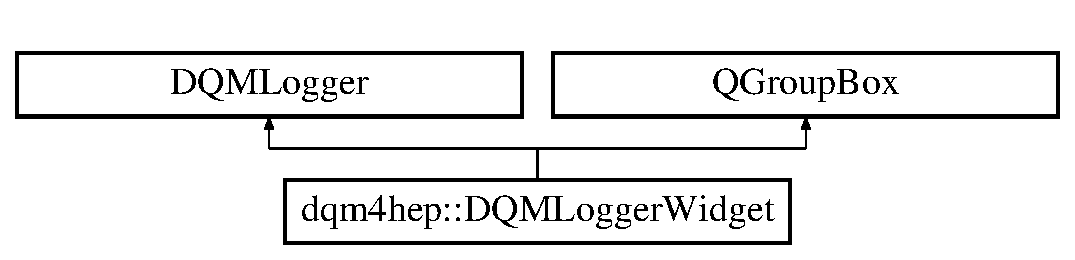
\includegraphics[height=2.000000cm]{classdqm4hep_1_1DQMLoggerWidget}
\end{center}
\end{figure}
\subsection*{Public Member Functions}
\begin{DoxyCompactItemize}
\item 
{\bf D\+Q\+M\+Logger\+Widget} (Q\+Widget $\ast$p\+Parent=0)
\begin{DoxyCompactList}\small\item\em Constructor. \end{DoxyCompactList}\item 
void {\bf log} (const std\+::string \&message)
\begin{DoxyCompactList}\small\item\em Log a message with the default level (M\+E\+S\+S\+A\+G\+E) \end{DoxyCompactList}\item 
void {\bf log} (Log\+Level level, const std\+::string \&message)
\begin{DoxyCompactList}\small\item\em Log a message with a log level. \end{DoxyCompactList}\end{DoxyCompactItemize}
\subsection*{Private Member Functions}
\begin{DoxyCompactItemize}
\item 
Qt\+::\+Global\+Color {\bf get\+Color} (Log\+Level level) const 
\item 
std\+::string {\bf get\+Log\+Message\+Head} (Log\+Level level) const 
\end{DoxyCompactItemize}
\subsection*{Private Attributes}
\begin{DoxyCompactItemize}
\item 
Q\+Text\+Edit $\ast$ {\bf m\+\_\+p\+Logging\+Widget}
\begin{DoxyCompactList}\small\item\em the text widget used for logging \end{DoxyCompactList}\end{DoxyCompactItemize}


\subsection{Detailed Description}
\doxyref{D\+Q\+M\+Logger\+Widget}{p.}{classdqm4hep_1_1DQMLoggerWidget} class. 

Definition at line 46 of file D\+Q\+M\+Logger\+Widget.\+h.



\subsection{Constructor \& Destructor Documentation}
\index{dqm4hep\+::\+D\+Q\+M\+Logger\+Widget@{dqm4hep\+::\+D\+Q\+M\+Logger\+Widget}!D\+Q\+M\+Logger\+Widget@{D\+Q\+M\+Logger\+Widget}}
\index{D\+Q\+M\+Logger\+Widget@{D\+Q\+M\+Logger\+Widget}!dqm4hep\+::\+D\+Q\+M\+Logger\+Widget@{dqm4hep\+::\+D\+Q\+M\+Logger\+Widget}}
\subsubsection[{D\+Q\+M\+Logger\+Widget}]{\setlength{\rightskip}{0pt plus 5cm}dqm4hep\+::\+D\+Q\+M\+Logger\+Widget\+::\+D\+Q\+M\+Logger\+Widget (
\begin{DoxyParamCaption}
\item[{Q\+Widget $\ast$}]{p\+Parent = {\ttfamily 0}}
\end{DoxyParamCaption}
)}\label{classdqm4hep_1_1DQMLoggerWidget_aa879525504381e025bb02b932c12a1ec}


Constructor. 



Definition at line 38 of file D\+Q\+M\+Logger\+Widget.\+cc.



References m\+\_\+p\+Logging\+Widget.


\begin{DoxyCode}
38                                                  :
39     QGroupBox(\textcolor{stringliteral}{"Logging"}, pParent)
40 \{
41   setMaximumHeight(200);
42 
43   QHBoxLayout *pLoggingLayout = \textcolor{keyword}{new} QHBoxLayout();
44   setLayout(pLoggingLayout);
45 
46   m_pLoggingWidget = \textcolor{keyword}{new} QTextEdit();
47   m_pLoggingWidget->setReadOnly(\textcolor{keyword}{true});
48   pLoggingLayout->addWidget(m_pLoggingWidget);
49 \}
\end{DoxyCode}


\subsection{Member Function Documentation}
\index{dqm4hep\+::\+D\+Q\+M\+Logger\+Widget@{dqm4hep\+::\+D\+Q\+M\+Logger\+Widget}!get\+Color@{get\+Color}}
\index{get\+Color@{get\+Color}!dqm4hep\+::\+D\+Q\+M\+Logger\+Widget@{dqm4hep\+::\+D\+Q\+M\+Logger\+Widget}}
\subsubsection[{get\+Color}]{\setlength{\rightskip}{0pt plus 5cm}Qt\+::\+Global\+Color dqm4hep\+::\+D\+Q\+M\+Logger\+Widget\+::get\+Color (
\begin{DoxyParamCaption}
\item[{Log\+Level}]{level}
\end{DoxyParamCaption}
) const\hspace{0.3cm}{\ttfamily [private]}}\label{classdqm4hep_1_1DQMLoggerWidget_a4a3ce5fd8c585a5cafe842ad7637c6c5}


Definition at line 85 of file D\+Q\+M\+Logger\+Widget.\+cc.



Referenced by log().


\begin{DoxyCode}
86 \{
87   \textcolor{keywordflow}{switch} (level)
88   \{
89   \textcolor{keywordflow}{case} DEBUG :
90     \textcolor{keywordflow}{return} Qt::darkBlue;
91   \textcolor{keywordflow}{case} MESSAGE :
92     \textcolor{keywordflow}{return} Qt::darkGreen;
93   \textcolor{keywordflow}{case} WARNING :
94     \textcolor{keywordflow}{return} Qt::darkYellow;
95   \textcolor{keywordflow}{case} ERROR :
96     \textcolor{keywordflow}{return} Qt::darkRed;
97   \textcolor{keywordflow}{default}:
98     \textcolor{keywordflow}{return} Qt::black;
99   \}
100 \}
\end{DoxyCode}
\index{dqm4hep\+::\+D\+Q\+M\+Logger\+Widget@{dqm4hep\+::\+D\+Q\+M\+Logger\+Widget}!get\+Log\+Message\+Head@{get\+Log\+Message\+Head}}
\index{get\+Log\+Message\+Head@{get\+Log\+Message\+Head}!dqm4hep\+::\+D\+Q\+M\+Logger\+Widget@{dqm4hep\+::\+D\+Q\+M\+Logger\+Widget}}
\subsubsection[{get\+Log\+Message\+Head}]{\setlength{\rightskip}{0pt plus 5cm}std\+::string dqm4hep\+::\+D\+Q\+M\+Logger\+Widget\+::get\+Log\+Message\+Head (
\begin{DoxyParamCaption}
\item[{Log\+Level}]{level}
\end{DoxyParamCaption}
) const\hspace{0.3cm}{\ttfamily [private]}}\label{classdqm4hep_1_1DQMLoggerWidget_a3adbc75b7204f745a0e1c1c9b8e3f88f}


Definition at line 104 of file D\+Q\+M\+Logger\+Widget.\+cc.



Referenced by log().


\begin{DoxyCode}
105 \{
106   \textcolor{keywordflow}{switch} (level)
107   \{
108   \textcolor{keywordflow}{case} DEBUG :
109     \textcolor{keywordflow}{return} \textcolor{stringliteral}{"[DEBUG]       "};
110   \textcolor{keywordflow}{case} MESSAGE :
111     \textcolor{keywordflow}{return} \textcolor{stringliteral}{"[MESSAGE]  "};
112   \textcolor{keywordflow}{case} WARNING :
113     \textcolor{keywordflow}{return} \textcolor{stringliteral}{"[WARNING] "};
114   \textcolor{keywordflow}{case} ERROR :
115     \textcolor{keywordflow}{return} \textcolor{stringliteral}{"[ERROR]       "};
116   \textcolor{keywordflow}{default}:
117     \textcolor{keywordflow}{return} \textcolor{stringliteral}{""};
118   \}
119 \}
\end{DoxyCode}
\index{dqm4hep\+::\+D\+Q\+M\+Logger\+Widget@{dqm4hep\+::\+D\+Q\+M\+Logger\+Widget}!log@{log}}
\index{log@{log}!dqm4hep\+::\+D\+Q\+M\+Logger\+Widget@{dqm4hep\+::\+D\+Q\+M\+Logger\+Widget}}
\subsubsection[{log}]{\setlength{\rightskip}{0pt plus 5cm}void dqm4hep\+::\+D\+Q\+M\+Logger\+Widget\+::log (
\begin{DoxyParamCaption}
\item[{const std\+::string \&}]{message}
\end{DoxyParamCaption}
)}\label{classdqm4hep_1_1DQMLoggerWidget_a7a93d18aabd959b7d53aa14b8878f958}


Log a message with the default level (M\+E\+S\+S\+A\+G\+E) 



Definition at line 53 of file D\+Q\+M\+Logger\+Widget.\+cc.


\begin{DoxyCode}
54 \{
55   log(MESSAGE, message);
56 \}
\end{DoxyCode}
\index{dqm4hep\+::\+D\+Q\+M\+Logger\+Widget@{dqm4hep\+::\+D\+Q\+M\+Logger\+Widget}!log@{log}}
\index{log@{log}!dqm4hep\+::\+D\+Q\+M\+Logger\+Widget@{dqm4hep\+::\+D\+Q\+M\+Logger\+Widget}}
\subsubsection[{log}]{\setlength{\rightskip}{0pt plus 5cm}void dqm4hep\+::\+D\+Q\+M\+Logger\+Widget\+::log (
\begin{DoxyParamCaption}
\item[{Log\+Level}]{level, }
\item[{const std\+::string \&}]{message}
\end{DoxyParamCaption}
)}\label{classdqm4hep_1_1DQMLoggerWidget_a60db9e7e500d1accf17a7f05ffa51831}


Log a message with a log level. 



Definition at line 60 of file D\+Q\+M\+Logger\+Widget.\+cc.



References get\+Color(), get\+Log\+Message\+Head(), and m\+\_\+p\+Logging\+Widget.


\begin{DoxyCode}
61 \{
62   Qt::GlobalColor color = getColor(level);
63 
64   QString messageHead(getLogMessageHead(level).c\_str());
65 
66   \textcolor{comment}{// scroll to the end of text edit}
67   m_pLoggingWidget->horizontalScrollBar()->setValue(m_pLoggingWidget->horizontalScrollBar()->maximum());
68 
69   \textcolor{comment}{// set the cursor at the end}
70   QTextCursor cursor = m_pLoggingWidget->textCursor();
71   cursor.movePosition(QTextCursor::End, QTextCursor::MoveAnchor);
72   m_pLoggingWidget->setTextCursor(cursor);
73 
74   \textcolor{comment}{// put the message}
75   m_pLoggingWidget->setTextColor(QColor(color));
76   m_pLoggingWidget->insertPlainText(messageHead);
77   m_pLoggingWidget->setTextColor(QColor(Qt::black));
78   m_pLoggingWidget->insertPlainText(\textcolor{stringliteral}{" "});
79   m_pLoggingWidget->insertPlainText(QString(message.c\_str()));
80   m_pLoggingWidget->insertPlainText(\textcolor{stringliteral}{"\(\backslash\)n"});
81 \}
\end{DoxyCode}


\subsection{Member Data Documentation}
\index{dqm4hep\+::\+D\+Q\+M\+Logger\+Widget@{dqm4hep\+::\+D\+Q\+M\+Logger\+Widget}!m\+\_\+p\+Logging\+Widget@{m\+\_\+p\+Logging\+Widget}}
\index{m\+\_\+p\+Logging\+Widget@{m\+\_\+p\+Logging\+Widget}!dqm4hep\+::\+D\+Q\+M\+Logger\+Widget@{dqm4hep\+::\+D\+Q\+M\+Logger\+Widget}}
\subsubsection[{m\+\_\+p\+Logging\+Widget}]{\setlength{\rightskip}{0pt plus 5cm}Q\+Text\+Edit$\ast$ dqm4hep\+::\+D\+Q\+M\+Logger\+Widget\+::m\+\_\+p\+Logging\+Widget\hspace{0.3cm}{\ttfamily [private]}}\label{classdqm4hep_1_1DQMLoggerWidget_a1585de3aab0c62368e24a7a06fe7bcb4}


the text widget used for logging 



Definition at line 66 of file D\+Q\+M\+Logger\+Widget.\+h.



Referenced by D\+Q\+M\+Logger\+Widget(), and log().



The documentation for this class was generated from the following files\+:\begin{DoxyCompactItemize}
\item 
{\bf D\+Q\+M\+Logger\+Widget.\+h}\item 
{\bf D\+Q\+M\+Logger\+Widget.\+cc}\end{DoxyCompactItemize}

\section{dqm4hep\+:\+:D\+Q\+M\+Monitor\+Element\+Info\+Widget Class Reference}
\label{classdqm4hep_1_1DQMMonitorElementInfoWidget}\index{dqm4hep\+::\+D\+Q\+M\+Monitor\+Element\+Info\+Widget@{dqm4hep\+::\+D\+Q\+M\+Monitor\+Element\+Info\+Widget}}


\doxyref{D\+Q\+M\+Monitor\+Element\+Info\+Widget}{p.}{classdqm4hep_1_1DQMMonitorElementInfoWidget} class.  




{\ttfamily \#include $<$D\+Q\+M\+Monitor\+Element\+Info\+Widget.\+h$>$}

Inheritance diagram for dqm4hep\+:\+:D\+Q\+M\+Monitor\+Element\+Info\+Widget\+:\begin{figure}[H]
\begin{center}
\leavevmode
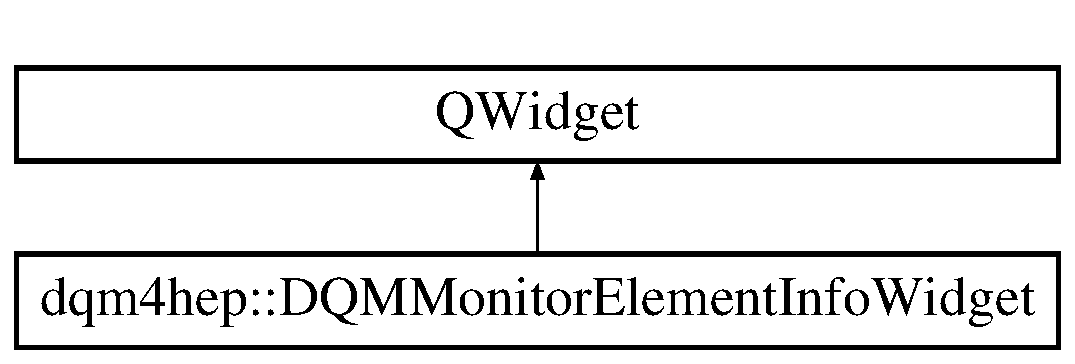
\includegraphics[height=2.000000cm]{classdqm4hep_1_1DQMMonitorElementInfoWidget}
\end{center}
\end{figure}
\subsection*{Public Types}
\begin{DoxyCompactItemize}
\item 
enum {\bf Tab} \{ {\bf M\+O\+N\+I\+T\+O\+R\+\_\+\+E\+L\+E\+M\+E\+N\+T\+\_\+\+I\+N\+F\+O} = 0, 
{\bf Q\+U\+A\+L\+I\+T\+Y\+\_\+\+T\+E\+S\+T\+\_\+\+R\+E\+S\+U\+L\+T\+S} = 1
 \}
\end{DoxyCompactItemize}
\subsection*{Public Member Functions}
\begin{DoxyCompactItemize}
\item 
{\bf D\+Q\+M\+Monitor\+Element\+Info\+Widget} (Q\+Widget $\ast$p\+Parent\+Widget=N\+U\+L\+L)
\begin{DoxyCompactList}\small\item\em Constructor. \end{DoxyCompactList}\item 
{\bf D\+Q\+M\+Monitor\+Element\+Info\+Widget} ({\bf D\+Q\+M\+Gui\+Monitor\+Element} $\ast$p\+Gui\+Monitor\+Element, Q\+Widget $\ast$p\+Parent\+Widget=N\+U\+L\+L)
\begin{DoxyCompactList}\small\item\em Constructor. \end{DoxyCompactList}\item 
{\bf $\sim$\+D\+Q\+M\+Monitor\+Element\+Info\+Widget} ()
\begin{DoxyCompactList}\small\item\em Destructor. \end{DoxyCompactList}\item 
void {\bf fill\+Infos} ({\bf D\+Q\+M\+Gui\+Monitor\+Element} $\ast$p\+Gui\+Monitor\+Element)
\begin{DoxyCompactList}\small\item\em Fill the widget information with the given monitor element. \end{DoxyCompactList}\item 
void {\bf show\+Tab} ({\bf Tab} tab)
\begin{DoxyCompactList}\small\item\em Show the given tab. \end{DoxyCompactList}\end{DoxyCompactItemize}
\subsection*{Private Slots}
\begin{DoxyCompactItemize}
\item 
void {\bf fill\+Infos} ()
\begin{DoxyCompactList}\small\item\em Fill the widget information. \end{DoxyCompactList}\item 
void {\bf load\+Quality\+Test\+Result} (int index)
\item 
void {\bf handle\+Update\+Check\+State\+Changed} (int state)
\end{DoxyCompactItemize}
\subsection*{Private Member Functions}
\begin{DoxyCompactItemize}
\item 
void {\bf build\+Widget} ()
\end{DoxyCompactItemize}
\subsection*{Private Attributes}
\begin{DoxyCompactItemize}
\item 
Q\+Check\+Box $\ast$ {\bf m\+\_\+p\+Update\+Box}
\item 
Q\+Tab\+Widget $\ast$ {\bf m\+\_\+p\+Tab\+Widget}
\item 
Q\+Label $\ast$ {\bf m\+\_\+p\+Monitor\+Element\+Name\+Label}
\item 
Q\+Label $\ast$ {\bf m\+\_\+p\+Monitor\+Element\+Title\+Label}
\item 
Q\+Label $\ast$ {\bf m\+\_\+p\+Monitor\+Element\+Type\+Label}
\item 
Q\+Label $\ast$ {\bf m\+\_\+p\+Monitor\+Element\+Reset\+Policy\+Label}
\item 
Q\+Text\+Edit $\ast$ {\bf m\+\_\+p\+Monitor\+Element\+Description\+Text\+Edit}
\item 
Q\+Label $\ast$ {\bf m\+\_\+p\+Monitor\+Element\+Draw\+Option\+Label}
\item 
Q\+Label $\ast$ {\bf m\+\_\+p\+Monitor\+Element\+Run\+Number\+Label}
\item 
Q\+Label $\ast$ {\bf m\+\_\+p\+Monitor\+Element\+Full\+Path\+Label}
\item 
Q\+Label $\ast$ {\bf m\+\_\+p\+N\+Q\+Tests\+Label}
\item 
Q\+Label $\ast$ {\bf m\+\_\+p\+N\+Success\+Q\+Tests\+Label}
\item 
Q\+Label $\ast$ {\bf m\+\_\+p\+N\+Fail\+Q\+Tests\+Label}
\item 
Q\+Label $\ast$ {\bf m\+\_\+p\+Mean\+Quality\+Q\+Tests\+Label}
\item 
Q\+Combo\+Box $\ast$ {\bf m\+\_\+p\+Q\+Tests\+Combo\+Box}
\item 
Q\+Label $\ast$ {\bf m\+\_\+p\+Quality\+Test\+Type\+Label}
\item 
Q\+Text\+Edit $\ast$ {\bf m\+\_\+p\+Quality\+Test\+Message\+Edit}
\item 
Q\+Label $\ast$ {\bf m\+\_\+p\+Quality\+Test\+Quality\+Label}
\item 
Q\+Label $\ast$ {\bf m\+\_\+p\+Quality\+Test\+Success\+Label}
\item 
std\+::map$<$ std\+::string, \\*
D\+Q\+M\+Quality\+Test\+Result $>$ {\bf m\+\_\+quality\+Test\+Result\+Map}
\item 
{\bf D\+Q\+M\+Gui\+Monitor\+Element} $\ast$ {\bf m\+\_\+p\+Gui\+Monitor\+Element}
\end{DoxyCompactItemize}


\subsection{Detailed Description}
\doxyref{D\+Q\+M\+Monitor\+Element\+Info\+Widget}{p.}{classdqm4hep_1_1DQMMonitorElementInfoWidget} class. 

Definition at line 56 of file D\+Q\+M\+Monitor\+Element\+Info\+Widget.\+h.



\subsection{Member Enumeration Documentation}
\index{dqm4hep\+::\+D\+Q\+M\+Monitor\+Element\+Info\+Widget@{dqm4hep\+::\+D\+Q\+M\+Monitor\+Element\+Info\+Widget}!Tab@{Tab}}
\index{Tab@{Tab}!dqm4hep\+::\+D\+Q\+M\+Monitor\+Element\+Info\+Widget@{dqm4hep\+::\+D\+Q\+M\+Monitor\+Element\+Info\+Widget}}
\subsubsection[{Tab}]{\setlength{\rightskip}{0pt plus 5cm}enum {\bf dqm4hep\+::\+D\+Q\+M\+Monitor\+Element\+Info\+Widget\+::\+Tab}}\label{classdqm4hep_1_1DQMMonitorElementInfoWidget_a4578459f3077efd1dcac7f5ff121f79d}
\begin{Desc}
\item[Enumerator]\par
\begin{description}
\index{M\+O\+N\+I\+T\+O\+R\+\_\+\+E\+L\+E\+M\+E\+N\+T\+\_\+\+I\+N\+F\+O@{M\+O\+N\+I\+T\+O\+R\+\_\+\+E\+L\+E\+M\+E\+N\+T\+\_\+\+I\+N\+F\+O}!dqm4hep\+::\+D\+Q\+M\+Monitor\+Element\+Info\+Widget@{dqm4hep\+::\+D\+Q\+M\+Monitor\+Element\+Info\+Widget}}\index{dqm4hep\+::\+D\+Q\+M\+Monitor\+Element\+Info\+Widget@{dqm4hep\+::\+D\+Q\+M\+Monitor\+Element\+Info\+Widget}!M\+O\+N\+I\+T\+O\+R\+\_\+\+E\+L\+E\+M\+E\+N\+T\+\_\+\+I\+N\+F\+O@{M\+O\+N\+I\+T\+O\+R\+\_\+\+E\+L\+E\+M\+E\+N\+T\+\_\+\+I\+N\+F\+O}}\item[{\em 
M\+O\+N\+I\+T\+O\+R\+\_\+\+E\+L\+E\+M\+E\+N\+T\+\_\+\+I\+N\+F\+O\label{classdqm4hep_1_1DQMMonitorElementInfoWidget_a4578459f3077efd1dcac7f5ff121f79da7d31e08e0a6031324c6a060e75fd7531}
}]\index{Q\+U\+A\+L\+I\+T\+Y\+\_\+\+T\+E\+S\+T\+\_\+\+R\+E\+S\+U\+L\+T\+S@{Q\+U\+A\+L\+I\+T\+Y\+\_\+\+T\+E\+S\+T\+\_\+\+R\+E\+S\+U\+L\+T\+S}!dqm4hep\+::\+D\+Q\+M\+Monitor\+Element\+Info\+Widget@{dqm4hep\+::\+D\+Q\+M\+Monitor\+Element\+Info\+Widget}}\index{dqm4hep\+::\+D\+Q\+M\+Monitor\+Element\+Info\+Widget@{dqm4hep\+::\+D\+Q\+M\+Monitor\+Element\+Info\+Widget}!Q\+U\+A\+L\+I\+T\+Y\+\_\+\+T\+E\+S\+T\+\_\+\+R\+E\+S\+U\+L\+T\+S@{Q\+U\+A\+L\+I\+T\+Y\+\_\+\+T\+E\+S\+T\+\_\+\+R\+E\+S\+U\+L\+T\+S}}\item[{\em 
Q\+U\+A\+L\+I\+T\+Y\+\_\+\+T\+E\+S\+T\+\_\+\+R\+E\+S\+U\+L\+T\+S\label{classdqm4hep_1_1DQMMonitorElementInfoWidget_a4578459f3077efd1dcac7f5ff121f79dac705f40eaf88945c6c4db9b7579924ed}
}]\end{description}
\end{Desc}


Definition at line 62 of file D\+Q\+M\+Monitor\+Element\+Info\+Widget.\+h.


\begin{DoxyCode}
63   \{
64     MONITOR_ELEMENT_INFO = 0,
65     QUALITY_TEST_RESULTS = 1
66   \};
\end{DoxyCode}


\subsection{Constructor \& Destructor Documentation}
\index{dqm4hep\+::\+D\+Q\+M\+Monitor\+Element\+Info\+Widget@{dqm4hep\+::\+D\+Q\+M\+Monitor\+Element\+Info\+Widget}!D\+Q\+M\+Monitor\+Element\+Info\+Widget@{D\+Q\+M\+Monitor\+Element\+Info\+Widget}}
\index{D\+Q\+M\+Monitor\+Element\+Info\+Widget@{D\+Q\+M\+Monitor\+Element\+Info\+Widget}!dqm4hep\+::\+D\+Q\+M\+Monitor\+Element\+Info\+Widget@{dqm4hep\+::\+D\+Q\+M\+Monitor\+Element\+Info\+Widget}}
\subsubsection[{D\+Q\+M\+Monitor\+Element\+Info\+Widget}]{\setlength{\rightskip}{0pt plus 5cm}dqm4hep\+::\+D\+Q\+M\+Monitor\+Element\+Info\+Widget\+::\+D\+Q\+M\+Monitor\+Element\+Info\+Widget (
\begin{DoxyParamCaption}
\item[{Q\+Widget $\ast$}]{p\+Parent\+Widget = {\ttfamily NULL}}
\end{DoxyParamCaption}
)}\label{classdqm4hep_1_1DQMMonitorElementInfoWidget_a6afd30953bc7e3c93bd32a3018bd8eeb}


Constructor. 



Definition at line 44 of file D\+Q\+M\+Monitor\+Element\+Info\+Widget.\+cc.



References build\+Widget().


\begin{DoxyCode}
44                                                                                :
45     QWidget(pParentWidget),
46     m_pGuiMonitorElement(0)
47 \{
48   buildWidget();
49 \}
\end{DoxyCode}
\index{dqm4hep\+::\+D\+Q\+M\+Monitor\+Element\+Info\+Widget@{dqm4hep\+::\+D\+Q\+M\+Monitor\+Element\+Info\+Widget}!D\+Q\+M\+Monitor\+Element\+Info\+Widget@{D\+Q\+M\+Monitor\+Element\+Info\+Widget}}
\index{D\+Q\+M\+Monitor\+Element\+Info\+Widget@{D\+Q\+M\+Monitor\+Element\+Info\+Widget}!dqm4hep\+::\+D\+Q\+M\+Monitor\+Element\+Info\+Widget@{dqm4hep\+::\+D\+Q\+M\+Monitor\+Element\+Info\+Widget}}
\subsubsection[{D\+Q\+M\+Monitor\+Element\+Info\+Widget}]{\setlength{\rightskip}{0pt plus 5cm}dqm4hep\+::\+D\+Q\+M\+Monitor\+Element\+Info\+Widget\+::\+D\+Q\+M\+Monitor\+Element\+Info\+Widget (
\begin{DoxyParamCaption}
\item[{{\bf D\+Q\+M\+Gui\+Monitor\+Element} $\ast$}]{p\+Gui\+Monitor\+Element, }
\item[{Q\+Widget $\ast$}]{p\+Parent\+Widget = {\ttfamily NULL}}
\end{DoxyParamCaption}
)}\label{classdqm4hep_1_1DQMMonitorElementInfoWidget_a5415914418e50fc051267475f7205c4e}


Constructor. 



Definition at line 34 of file D\+Q\+M\+Monitor\+Element\+Info\+Widget.\+cc.



References build\+Widget(), and fill\+Infos().


\begin{DoxyCode}
34                                                                                                            
                    :
35     QWidget(pParentWidget),
36     m_pGuiMonitorElement(pGuiMonitorElement)
37 \{
38   buildWidget();
39   fillInfos(pGuiMonitorElement);
40 \}
\end{DoxyCode}
\index{dqm4hep\+::\+D\+Q\+M\+Monitor\+Element\+Info\+Widget@{dqm4hep\+::\+D\+Q\+M\+Monitor\+Element\+Info\+Widget}!````~D\+Q\+M\+Monitor\+Element\+Info\+Widget@{$\sim$\+D\+Q\+M\+Monitor\+Element\+Info\+Widget}}
\index{````~D\+Q\+M\+Monitor\+Element\+Info\+Widget@{$\sim$\+D\+Q\+M\+Monitor\+Element\+Info\+Widget}!dqm4hep\+::\+D\+Q\+M\+Monitor\+Element\+Info\+Widget@{dqm4hep\+::\+D\+Q\+M\+Monitor\+Element\+Info\+Widget}}
\subsubsection[{$\sim$\+D\+Q\+M\+Monitor\+Element\+Info\+Widget}]{\setlength{\rightskip}{0pt plus 5cm}dqm4hep\+::\+D\+Q\+M\+Monitor\+Element\+Info\+Widget\+::$\sim$\+D\+Q\+M\+Monitor\+Element\+Info\+Widget (
\begin{DoxyParamCaption}
{}
\end{DoxyParamCaption}
)}\label{classdqm4hep_1_1DQMMonitorElementInfoWidget_a2786d9f0c54fc8c59717f02377642503}


Destructor. 



Definition at line 53 of file D\+Q\+M\+Monitor\+Element\+Info\+Widget.\+cc.


\begin{DoxyCode}
54 \{
55   \textcolor{comment}{/* nop */}
56 \}
\end{DoxyCode}


\subsection{Member Function Documentation}
\index{dqm4hep\+::\+D\+Q\+M\+Monitor\+Element\+Info\+Widget@{dqm4hep\+::\+D\+Q\+M\+Monitor\+Element\+Info\+Widget}!build\+Widget@{build\+Widget}}
\index{build\+Widget@{build\+Widget}!dqm4hep\+::\+D\+Q\+M\+Monitor\+Element\+Info\+Widget@{dqm4hep\+::\+D\+Q\+M\+Monitor\+Element\+Info\+Widget}}
\subsubsection[{build\+Widget}]{\setlength{\rightskip}{0pt plus 5cm}void dqm4hep\+::\+D\+Q\+M\+Monitor\+Element\+Info\+Widget\+::build\+Widget (
\begin{DoxyParamCaption}
{}
\end{DoxyParamCaption}
)\hspace{0.3cm}{\ttfamily [private]}}\label{classdqm4hep_1_1DQMMonitorElementInfoWidget_a851ba871f62718864571d911afd3356f}


Definition at line 67 of file D\+Q\+M\+Monitor\+Element\+Info\+Widget.\+cc.



References handle\+Update\+Check\+State\+Changed(), load\+Quality\+Test\+Result(), m\+\_\+p\+Mean\+Quality\+Q\+Tests\+Label, m\+\_\+p\+Monitor\+Element\+Description\+Text\+Edit, m\+\_\+p\+Monitor\+Element\+Draw\+Option\+Label, m\+\_\+p\+Monitor\+Element\+Full\+Path\+Label, m\+\_\+p\+Monitor\+Element\+Name\+Label, m\+\_\+p\+Monitor\+Element\+Reset\+Policy\+Label, m\+\_\+p\+Monitor\+Element\+Run\+Number\+Label, m\+\_\+p\+Monitor\+Element\+Title\+Label, m\+\_\+p\+Monitor\+Element\+Type\+Label, m\+\_\+p\+N\+Fail\+Q\+Tests\+Label, m\+\_\+p\+N\+Q\+Tests\+Label, m\+\_\+p\+N\+Success\+Q\+Tests\+Label, m\+\_\+p\+Q\+Tests\+Combo\+Box, m\+\_\+p\+Quality\+Test\+Message\+Edit, m\+\_\+p\+Quality\+Test\+Quality\+Label, m\+\_\+p\+Quality\+Test\+Success\+Label, m\+\_\+p\+Quality\+Test\+Type\+Label, m\+\_\+p\+Tab\+Widget, and m\+\_\+p\+Update\+Box.



Referenced by D\+Q\+M\+Monitor\+Element\+Info\+Widget().


\begin{DoxyCode}
68 \{
69   QVBoxLayout *pMainLayout = \textcolor{keyword}{new} QVBoxLayout();
70   setLayout(pMainLayout);
71 
72   m_pUpdateBox = \textcolor{keyword}{new} QCheckBox(\textcolor{stringliteral}{"Update info on monitor element update"});
73   m_pUpdateBox->setCheckState(Qt::Unchecked);
74 
75   pMainLayout->addWidget(m_pUpdateBox);
76 
77   m_pTabWidget = \textcolor{keyword}{new} QTabWidget();
78   pMainLayout->addWidget(m_pTabWidget);
79 
80   \textcolor{comment}{// description tab}
81   QWidget *pDescriptionTab = \textcolor{keyword}{new} QWidget();
82   QFormLayout *pDescriptionLayout = \textcolor{keyword}{new} QFormLayout();
83   pDescriptionTab->setLayout(pDescriptionLayout);
84 
85   m_pMonitorElementNameLabel = \textcolor{keyword}{new} QLabel();
86   pDescriptionLayout->addRow(\textcolor{stringliteral}{"Name : "}, m_pMonitorElementNameLabel);
87 
88   m_pMonitorElementTitleLabel = \textcolor{keyword}{new} QLabel();
89   pDescriptionLayout->addRow(\textcolor{stringliteral}{"Title : "}, m_pMonitorElementTitleLabel);
90 
91   m_pMonitorElementTypeLabel = \textcolor{keyword}{new} QLabel();
92   pDescriptionLayout->addRow(\textcolor{stringliteral}{"Type : "}, m_pMonitorElementTypeLabel);
93 
94   m_pMonitorElementResetPolicyLabel = \textcolor{keyword}{new} QLabel();
95   pDescriptionLayout->addRow(\textcolor{stringliteral}{"Reset policy : "}, 
      m_pMonitorElementResetPolicyLabel);
96 
97   m_pMonitorElementDescriptionTextEdit = \textcolor{keyword}{new} QTextEdit();
98   m_pMonitorElementDescriptionTextEdit->setReadOnly(\textcolor{keyword}{true});
99   pDescriptionLayout->addRow(\textcolor{stringliteral}{"Description : "}, 
      m_pMonitorElementDescriptionTextEdit);
100 
101   m_pMonitorElementDrawOptionLabel = \textcolor{keyword}{new} QLabel();
102   pDescriptionLayout->addRow(\textcolor{stringliteral}{"Draw option : "}, m_pMonitorElementDrawOptionLabel);
103 
104   m_pMonitorElementRunNumberLabel = \textcolor{keyword}{new} QLabel();
105   pDescriptionLayout->addRow(\textcolor{stringliteral}{"Run number : "}, m_pMonitorElementRunNumberLabel);
106 
107   m_pMonitorElementFullPathLabel = \textcolor{keyword}{new} QLabel();
108   pDescriptionLayout->addRow(\textcolor{stringliteral}{"Full path : "}, m_pMonitorElementFullPathLabel);
109 
110   m_pTabWidget->addTab(pDescriptionTab, \textcolor{stringliteral}{"Description"});
111 
112   \textcolor{comment}{// quality test tab}
113   QWidget *pQualityTestTab = \textcolor{keyword}{new} QWidget();
114 
115   QVBoxLayout *pQualityTestLayout = \textcolor{keyword}{new} QVBoxLayout();
116   pQualityTestTab->setLayout(pQualityTestLayout);
117 
118   \textcolor{comment}{// global q test results}
119   QGroupBox *pGlobalQTestGroupBox = \textcolor{keyword}{new} QGroupBox(\textcolor{stringliteral}{"Global"});
120   QFormLayout *pGlobalQTestLayout = \textcolor{keyword}{new} QFormLayout();
121   pGlobalQTestGroupBox->setLayout(pGlobalQTestLayout);
122 
123   \textcolor{comment}{// fill the global q test area}
124   m_pNQTestsLabel = \textcolor{keyword}{new} QLabel();
125   pGlobalQTestLayout->addRow(\textcolor{stringliteral}{"Number of quality tests : "}, m_pNQTestsLabel);
126 
127   m_pNSuccessQTestsLabel = \textcolor{keyword}{new} QLabel();
128   m_pNSuccessQTestsLabel->setStyleSheet(\textcolor{stringliteral}{"QLabel \{ color: green; \}"});
129   pGlobalQTestLayout->addRow(\textcolor{stringliteral}{"Number of successes : "}, m_pNSuccessQTestsLabel);
130 
131   m_pNFailQTestsLabel = \textcolor{keyword}{new} QLabel();
132   m_pNFailQTestsLabel->setStyleSheet(\textcolor{stringliteral}{"QLabel \{ color: red; \}"});
133   pGlobalQTestLayout->addRow(\textcolor{stringliteral}{"Number of fails : "}, m_pNFailQTestsLabel);
134 
135   m_pMeanQualityQTestsLabel = \textcolor{keyword}{new} QLabel();
136   pGlobalQTestLayout->addRow(\textcolor{stringliteral}{"Mean quality : "}, m_pMeanQualityQTestsLabel);
137 
138   pQualityTestLayout->addWidget(pGlobalQTestGroupBox);
139 
140   \textcolor{comment}{// detailed view of quality tests}
141   QGroupBox *pDetailQTestGroupBox = \textcolor{keyword}{new} QGroupBox(\textcolor{stringliteral}{"Detail"});
142   QFormLayout *pDetailQTestLayout = \textcolor{keyword}{new} QFormLayout();
143   pDetailQTestGroupBox->setLayout(pDetailQTestLayout);
144 
145   m_pQTestsComboBox = \textcolor{keyword}{new} QComboBox();
146   pDetailQTestLayout->addRow(\textcolor{stringliteral}{"Quality test : "}, m_pQTestsComboBox);
147 
148   m_pQualityTestTypeLabel = \textcolor{keyword}{new} QLabel();
149   pDetailQTestLayout->addRow(\textcolor{stringliteral}{"Type : "}, m_pQualityTestTypeLabel);
150 
151   m_pQualityTestMessageEdit = \textcolor{keyword}{new} QTextEdit();
152   m_pQualityTestMessageEdit->setReadOnly(\textcolor{keyword}{true});
153   pDetailQTestLayout->addRow(\textcolor{stringliteral}{"Message : "}, m_pQualityTestMessageEdit);
154 
155   m_pQualityTestQualityLabel = \textcolor{keyword}{new} QLabel();
156   pDetailQTestLayout->addRow(\textcolor{stringliteral}{"Quality : "}, m_pQualityTestQualityLabel);
157 
158   m_pQualityTestSuccessLabel = \textcolor{keyword}{new} QLabel();
159   pDetailQTestLayout->addRow(\textcolor{stringliteral}{"Success : "}, m_pQualityTestSuccessLabel);
160 
161   pQualityTestLayout->addWidget(pDetailQTestGroupBox);
162 
163   m_pTabWidget->addTab(pQualityTestTab, \textcolor{stringliteral}{"Quality tests"});
164 
165   connect(m_pQTestsComboBox, SIGNAL(currentIndexChanged(\textcolor{keywordtype}{int})), \textcolor{keyword}{this}, SLOT(
      loadQualityTestResult(\textcolor{keywordtype}{int})));
166   connect(m_pUpdateBox, SIGNAL(stateChanged(\textcolor{keywordtype}{int})), \textcolor{keyword}{this}, SLOT(
      handleUpdateCheckStateChanged(\textcolor{keywordtype}{int})));
167 \}
\end{DoxyCode}
\index{dqm4hep\+::\+D\+Q\+M\+Monitor\+Element\+Info\+Widget@{dqm4hep\+::\+D\+Q\+M\+Monitor\+Element\+Info\+Widget}!fill\+Infos@{fill\+Infos}}
\index{fill\+Infos@{fill\+Infos}!dqm4hep\+::\+D\+Q\+M\+Monitor\+Element\+Info\+Widget@{dqm4hep\+::\+D\+Q\+M\+Monitor\+Element\+Info\+Widget}}
\subsubsection[{fill\+Infos}]{\setlength{\rightskip}{0pt plus 5cm}void dqm4hep\+::\+D\+Q\+M\+Monitor\+Element\+Info\+Widget\+::fill\+Infos (
\begin{DoxyParamCaption}
\item[{{\bf D\+Q\+M\+Gui\+Monitor\+Element} $\ast$}]{p\+Gui\+Monitor\+Element}
\end{DoxyParamCaption}
)}\label{classdqm4hep_1_1DQMMonitorElementInfoWidget_a9ffadabd4e75410c5e0411e142122aa3}


Fill the widget information with the given monitor element. 



Definition at line 178 of file D\+Q\+M\+Monitor\+Element\+Info\+Widget.\+cc.



References dqm4hep\+::\+D\+Q\+M\+Gui\+Monitor\+Element\+::get\+Monitor\+Element(), load\+Quality\+Test\+Result(), m\+\_\+p\+Mean\+Quality\+Q\+Tests\+Label, m\+\_\+p\+Monitor\+Element\+Description\+Text\+Edit, m\+\_\+p\+Monitor\+Element\+Draw\+Option\+Label, m\+\_\+p\+Monitor\+Element\+Full\+Path\+Label, m\+\_\+p\+Monitor\+Element\+Name\+Label, m\+\_\+p\+Monitor\+Element\+Reset\+Policy\+Label, m\+\_\+p\+Monitor\+Element\+Run\+Number\+Label, m\+\_\+p\+Monitor\+Element\+Title\+Label, m\+\_\+p\+Monitor\+Element\+Type\+Label, m\+\_\+p\+N\+Fail\+Q\+Tests\+Label, m\+\_\+p\+N\+Q\+Tests\+Label, m\+\_\+p\+N\+Success\+Q\+Tests\+Label, m\+\_\+p\+Q\+Tests\+Combo\+Box, and m\+\_\+quality\+Test\+Result\+Map.


\begin{DoxyCode}
179 \{
180   \textcolor{keywordflow}{if}(NULL == pGuiMonitorElement)
181     \textcolor{keywordflow}{return};
182 
183   DQMMonitorElement *pMonitorElement = pGuiMonitorElement->getMonitorElement();
184 
185   \textcolor{keywordflow}{if}(NULL == pMonitorElement)
186     \textcolor{keywordflow}{return};
187 
188   \textcolor{comment}{//}
189   \textcolor{comment}{// Global infos}
190   \textcolor{comment}{//}
191   \textcolor{comment}{// name}
192   m_pMonitorElementNameLabel->setText(QString(pMonitorElement->getName().c\_str()));
193 
194   \textcolor{comment}{//title}
195   m_pMonitorElementTitleLabel->setText(QString(pMonitorElement->getTitle().c\_str()));
196 
197   \textcolor{comment}{// type}
198   m_pMonitorElementTypeLabel->setText(QString(monitorElementTypeToString(pMonitorElement->getType()).c\_str(
      )));
199 
200   \textcolor{comment}{// reset policy}
201   m_pMonitorElementResetPolicyLabel->setText(QString(resetPolicyToString(pMonitorElement->getResetPolicy())
      .c\_str()));
202 
203   \textcolor{comment}{// description}
204   m_pMonitorElementDescriptionTextEdit->clear();
205   m_pMonitorElementDescriptionTextEdit->append(QString(pMonitorElement->getDescription().c\_str()));
206 
207   \textcolor{comment}{// draw option}
208   m_pMonitorElementDrawOptionLabel->setText(QString(pMonitorElement->getDrawOption().c\_str()));
209 
210   \textcolor{comment}{// run number}
211   m_pMonitorElementRunNumberLabel->setText(QString::number(pMonitorElement->getRunNumber()));
212 
213   \textcolor{comment}{// full path}
214   m_pMonitorElementFullPathLabel->setText(QString(pMonitorElement->getPath().getPath().c\_str()));
215 
216   \textcolor{comment}{//}
217   \textcolor{comment}{// Q tests}
218   \textcolor{comment}{//}
219   m_qualityTestResultMap = pMonitorElement->getQualityTestResults();
220   m_pQTestsComboBox->clear();
221 
222   \textcolor{keywordtype}{unsigned} \textcolor{keywordtype}{int} nSuccess = 0;
223   \textcolor{keywordtype}{unsigned} \textcolor{keywordtype}{int} nFail = 0;
224   \textcolor{keywordtype}{float} meanQuality = 0.f;
225 
226   \textcolor{keywordflow}{for}(std::map<std::string, DQMQualityTestResult>::const\_iterator iter = 
      m_qualityTestResultMap.begin(),
227       endIter = m_qualityTestResultMap.end() ; endIter != iter ; ++iter)
228   \{
229     m_pQTestsComboBox->addItem(QString(iter->first.c\_str()));
230 
231     \textcolor{keywordflow}{if}(iter->second.m\_isSuccessful)
232       nSuccess++;
233     \textcolor{keywordflow}{else}
234       nFail++;
235 
236     meanQuality += \textcolor{keyword}{static\_cast<}\textcolor{keywordtype}{int}\textcolor{keyword}{>}(iter->second.m\_quality);
237   \}
238 
239   \textcolor{comment}{// n quality tests}
240   m_pNQTestsLabel->setText(QString::number(m_qualityTestResultMap.size()));
241 
242   \textcolor{comment}{// n successful q tests}
243   m_pNSuccessQTestsLabel->setText(QString::number(nSuccess));
244 
245   \textcolor{comment}{// n failed q tests}
246   m_pNFailQTestsLabel->setText(QString::number(nFail));
247 
248   \textcolor{keywordflow}{if}(!m_qualityTestResultMap.empty())
249   \{
250     meanQuality /= m_qualityTestResultMap.size();
251 
252     \textcolor{comment}{// mean quality rate}
253     m_pMeanQualityQTestsLabel->setText(QString::number(meanQuality) + \textcolor{stringliteral}{" / 5"});
254 
255     loadQualityTestResult(0);
256   \}
257   \textcolor{keywordflow}{else}
258   \{
259     m_pMeanQualityQTestsLabel->setText(\textcolor{stringliteral}{"NONE"});
260   \}
261 \}
\end{DoxyCode}
\index{dqm4hep\+::\+D\+Q\+M\+Monitor\+Element\+Info\+Widget@{dqm4hep\+::\+D\+Q\+M\+Monitor\+Element\+Info\+Widget}!fill\+Infos@{fill\+Infos}}
\index{fill\+Infos@{fill\+Infos}!dqm4hep\+::\+D\+Q\+M\+Monitor\+Element\+Info\+Widget@{dqm4hep\+::\+D\+Q\+M\+Monitor\+Element\+Info\+Widget}}
\subsubsection[{fill\+Infos}]{\setlength{\rightskip}{0pt plus 5cm}void dqm4hep\+::\+D\+Q\+M\+Monitor\+Element\+Info\+Widget\+::fill\+Infos (
\begin{DoxyParamCaption}
{}
\end{DoxyParamCaption}
)\hspace{0.3cm}{\ttfamily [private]}, {\ttfamily [slot]}}\label{classdqm4hep_1_1DQMMonitorElementInfoWidget_a6cce3cd9043184053f3a4e97febfc5c6}


Fill the widget information. 



Definition at line 171 of file D\+Q\+M\+Monitor\+Element\+Info\+Widget.\+cc.



References m\+\_\+p\+Gui\+Monitor\+Element.



Referenced by D\+Q\+M\+Monitor\+Element\+Info\+Widget(), and handle\+Update\+Check\+State\+Changed().


\begin{DoxyCode}
172 \{
173   fillInfos(m_pGuiMonitorElement);
174 \}
\end{DoxyCode}
\index{dqm4hep\+::\+D\+Q\+M\+Monitor\+Element\+Info\+Widget@{dqm4hep\+::\+D\+Q\+M\+Monitor\+Element\+Info\+Widget}!handle\+Update\+Check\+State\+Changed@{handle\+Update\+Check\+State\+Changed}}
\index{handle\+Update\+Check\+State\+Changed@{handle\+Update\+Check\+State\+Changed}!dqm4hep\+::\+D\+Q\+M\+Monitor\+Element\+Info\+Widget@{dqm4hep\+::\+D\+Q\+M\+Monitor\+Element\+Info\+Widget}}
\subsubsection[{handle\+Update\+Check\+State\+Changed}]{\setlength{\rightskip}{0pt plus 5cm}void dqm4hep\+::\+D\+Q\+M\+Monitor\+Element\+Info\+Widget\+::handle\+Update\+Check\+State\+Changed (
\begin{DoxyParamCaption}
\item[{int}]{state}
\end{DoxyParamCaption}
)\hspace{0.3cm}{\ttfamily [private]}, {\ttfamily [slot]}}\label{classdqm4hep_1_1DQMMonitorElementInfoWidget_a8e90d7986706e3f8ad054b48ec12ed96}


Definition at line 285 of file D\+Q\+M\+Monitor\+Element\+Info\+Widget.\+cc.



References fill\+Infos(), and m\+\_\+p\+Gui\+Monitor\+Element.



Referenced by build\+Widget().


\begin{DoxyCode}
286 \{
287   \textcolor{keywordflow}{if}(!m_pGuiMonitorElement)
288     \textcolor{keywordflow}{return};
289 
290   \textcolor{keywordflow}{if}(state == Qt::Checked)
291   \{
292     connect(m_pGuiMonitorElement, SIGNAL(updated()), \textcolor{keyword}{this}, SLOT(fillInfos()), Qt::UniqueConnection);
293   \}
294   \textcolor{keywordflow}{else}
295   \{
296     disconnect(m_pGuiMonitorElement, SIGNAL(updated()), \textcolor{keyword}{this}, SLOT(fillInfos()));
297   \}
298 \}
\end{DoxyCode}
\index{dqm4hep\+::\+D\+Q\+M\+Monitor\+Element\+Info\+Widget@{dqm4hep\+::\+D\+Q\+M\+Monitor\+Element\+Info\+Widget}!load\+Quality\+Test\+Result@{load\+Quality\+Test\+Result}}
\index{load\+Quality\+Test\+Result@{load\+Quality\+Test\+Result}!dqm4hep\+::\+D\+Q\+M\+Monitor\+Element\+Info\+Widget@{dqm4hep\+::\+D\+Q\+M\+Monitor\+Element\+Info\+Widget}}
\subsubsection[{load\+Quality\+Test\+Result}]{\setlength{\rightskip}{0pt plus 5cm}void dqm4hep\+::\+D\+Q\+M\+Monitor\+Element\+Info\+Widget\+::load\+Quality\+Test\+Result (
\begin{DoxyParamCaption}
\item[{int}]{index}
\end{DoxyParamCaption}
)\hspace{0.3cm}{\ttfamily [private]}, {\ttfamily [slot]}}\label{classdqm4hep_1_1DQMMonitorElementInfoWidget_ac780537000592add90be8c61ea40ebae}


Definition at line 265 of file D\+Q\+M\+Monitor\+Element\+Info\+Widget.\+cc.



References m\+\_\+p\+Q\+Tests\+Combo\+Box, m\+\_\+p\+Quality\+Test\+Message\+Edit, m\+\_\+p\+Quality\+Test\+Quality\+Label, m\+\_\+p\+Quality\+Test\+Success\+Label, m\+\_\+p\+Quality\+Test\+Type\+Label, and m\+\_\+quality\+Test\+Result\+Map.



Referenced by build\+Widget(), and fill\+Infos().


\begin{DoxyCode}
266 \{
267   \textcolor{keywordflow}{if}(index < 0 || m\_pQTestsComboBox->count() == 0 || index >= m_pQTestsComboBox->count())
268     \textcolor{keywordflow}{return};
269 
270   \textcolor{comment}{// find the quality test result}
271   std::string qualityTestName = m_pQTestsComboBox->itemText(index).toStdString();
272   std::map<std::string, DQMQualityTestResult>::const\_iterator findIter = 
      m_qualityTestResultMap.find(qualityTestName);
273 
274   \textcolor{keywordflow}{if}(findIter == m_qualityTestResultMap.end())
275     \textcolor{keywordflow}{return};
276 
277   m_pQualityTestTypeLabel->setText(findIter->second.m\_qualityTestType.c\_str());
278   m_pQualityTestMessageEdit->clear();
279   m_pQualityTestMessageEdit->append(findIter->second.m\_message.c\_str());
280   m_pQualityTestQualityLabel->setText(qualityToString(findIter->second.m\_quality).c\_str());
281   m_pQualityTestSuccessLabel->setText(DQM4HEP::typeToString(findIter->second.m\_isSuccessful).c\_str());
282 \}
\end{DoxyCode}
\index{dqm4hep\+::\+D\+Q\+M\+Monitor\+Element\+Info\+Widget@{dqm4hep\+::\+D\+Q\+M\+Monitor\+Element\+Info\+Widget}!show\+Tab@{show\+Tab}}
\index{show\+Tab@{show\+Tab}!dqm4hep\+::\+D\+Q\+M\+Monitor\+Element\+Info\+Widget@{dqm4hep\+::\+D\+Q\+M\+Monitor\+Element\+Info\+Widget}}
\subsubsection[{show\+Tab}]{\setlength{\rightskip}{0pt plus 5cm}void dqm4hep\+::\+D\+Q\+M\+Monitor\+Element\+Info\+Widget\+::show\+Tab (
\begin{DoxyParamCaption}
\item[{{\bf Tab}}]{tab}
\end{DoxyParamCaption}
)}\label{classdqm4hep_1_1DQMMonitorElementInfoWidget_a501829f0c8799b81f63c46c4aebdcdc4}


Show the given tab. 



Definition at line 60 of file D\+Q\+M\+Monitor\+Element\+Info\+Widget.\+cc.



References m\+\_\+p\+Tab\+Widget.



Referenced by dqm4hep\+::\+D\+Q\+M\+Monitoring\+Controller\+::open\+Monitor\+Element\+Info(), and dqm4hep\+::\+D\+Q\+M\+Monitoring\+Controller\+::open\+Quality\+Test\+Results().


\begin{DoxyCode}
61 \{
62   m_pTabWidget->setCurrentIndex(tab);
63 \}
\end{DoxyCode}


\subsection{Member Data Documentation}
\index{dqm4hep\+::\+D\+Q\+M\+Monitor\+Element\+Info\+Widget@{dqm4hep\+::\+D\+Q\+M\+Monitor\+Element\+Info\+Widget}!m\+\_\+p\+Gui\+Monitor\+Element@{m\+\_\+p\+Gui\+Monitor\+Element}}
\index{m\+\_\+p\+Gui\+Monitor\+Element@{m\+\_\+p\+Gui\+Monitor\+Element}!dqm4hep\+::\+D\+Q\+M\+Monitor\+Element\+Info\+Widget@{dqm4hep\+::\+D\+Q\+M\+Monitor\+Element\+Info\+Widget}}
\subsubsection[{m\+\_\+p\+Gui\+Monitor\+Element}]{\setlength{\rightskip}{0pt plus 5cm}{\bf D\+Q\+M\+Gui\+Monitor\+Element}$\ast$ dqm4hep\+::\+D\+Q\+M\+Monitor\+Element\+Info\+Widget\+::m\+\_\+p\+Gui\+Monitor\+Element\hspace{0.3cm}{\ttfamily [private]}}\label{classdqm4hep_1_1DQMMonitorElementInfoWidget_ab6b68c27296cc274094aa8be9d45619a}


Definition at line 134 of file D\+Q\+M\+Monitor\+Element\+Info\+Widget.\+h.



Referenced by fill\+Infos(), and handle\+Update\+Check\+State\+Changed().

\index{dqm4hep\+::\+D\+Q\+M\+Monitor\+Element\+Info\+Widget@{dqm4hep\+::\+D\+Q\+M\+Monitor\+Element\+Info\+Widget}!m\+\_\+p\+Mean\+Quality\+Q\+Tests\+Label@{m\+\_\+p\+Mean\+Quality\+Q\+Tests\+Label}}
\index{m\+\_\+p\+Mean\+Quality\+Q\+Tests\+Label@{m\+\_\+p\+Mean\+Quality\+Q\+Tests\+Label}!dqm4hep\+::\+D\+Q\+M\+Monitor\+Element\+Info\+Widget@{dqm4hep\+::\+D\+Q\+M\+Monitor\+Element\+Info\+Widget}}
\subsubsection[{m\+\_\+p\+Mean\+Quality\+Q\+Tests\+Label}]{\setlength{\rightskip}{0pt plus 5cm}Q\+Label$\ast$ dqm4hep\+::\+D\+Q\+M\+Monitor\+Element\+Info\+Widget\+::m\+\_\+p\+Mean\+Quality\+Q\+Tests\+Label\hspace{0.3cm}{\ttfamily [private]}}\label{classdqm4hep_1_1DQMMonitorElementInfoWidget_acc3935d3a75e16ed5ea5740ae974677f}


Definition at line 124 of file D\+Q\+M\+Monitor\+Element\+Info\+Widget.\+h.



Referenced by build\+Widget(), and fill\+Infos().

\index{dqm4hep\+::\+D\+Q\+M\+Monitor\+Element\+Info\+Widget@{dqm4hep\+::\+D\+Q\+M\+Monitor\+Element\+Info\+Widget}!m\+\_\+p\+Monitor\+Element\+Description\+Text\+Edit@{m\+\_\+p\+Monitor\+Element\+Description\+Text\+Edit}}
\index{m\+\_\+p\+Monitor\+Element\+Description\+Text\+Edit@{m\+\_\+p\+Monitor\+Element\+Description\+Text\+Edit}!dqm4hep\+::\+D\+Q\+M\+Monitor\+Element\+Info\+Widget@{dqm4hep\+::\+D\+Q\+M\+Monitor\+Element\+Info\+Widget}}
\subsubsection[{m\+\_\+p\+Monitor\+Element\+Description\+Text\+Edit}]{\setlength{\rightskip}{0pt plus 5cm}Q\+Text\+Edit$\ast$ dqm4hep\+::\+D\+Q\+M\+Monitor\+Element\+Info\+Widget\+::m\+\_\+p\+Monitor\+Element\+Description\+Text\+Edit\hspace{0.3cm}{\ttfamily [private]}}\label{classdqm4hep_1_1DQMMonitorElementInfoWidget_aa9c9a3b5275eb0a3fb9aa05f90a28c8f}


Definition at line 115 of file D\+Q\+M\+Monitor\+Element\+Info\+Widget.\+h.



Referenced by build\+Widget(), and fill\+Infos().

\index{dqm4hep\+::\+D\+Q\+M\+Monitor\+Element\+Info\+Widget@{dqm4hep\+::\+D\+Q\+M\+Monitor\+Element\+Info\+Widget}!m\+\_\+p\+Monitor\+Element\+Draw\+Option\+Label@{m\+\_\+p\+Monitor\+Element\+Draw\+Option\+Label}}
\index{m\+\_\+p\+Monitor\+Element\+Draw\+Option\+Label@{m\+\_\+p\+Monitor\+Element\+Draw\+Option\+Label}!dqm4hep\+::\+D\+Q\+M\+Monitor\+Element\+Info\+Widget@{dqm4hep\+::\+D\+Q\+M\+Monitor\+Element\+Info\+Widget}}
\subsubsection[{m\+\_\+p\+Monitor\+Element\+Draw\+Option\+Label}]{\setlength{\rightskip}{0pt plus 5cm}Q\+Label$\ast$ dqm4hep\+::\+D\+Q\+M\+Monitor\+Element\+Info\+Widget\+::m\+\_\+p\+Monitor\+Element\+Draw\+Option\+Label\hspace{0.3cm}{\ttfamily [private]}}\label{classdqm4hep_1_1DQMMonitorElementInfoWidget_ab17f410b7a5740bc1884beea6d11e024}


Definition at line 116 of file D\+Q\+M\+Monitor\+Element\+Info\+Widget.\+h.



Referenced by build\+Widget(), and fill\+Infos().

\index{dqm4hep\+::\+D\+Q\+M\+Monitor\+Element\+Info\+Widget@{dqm4hep\+::\+D\+Q\+M\+Monitor\+Element\+Info\+Widget}!m\+\_\+p\+Monitor\+Element\+Full\+Path\+Label@{m\+\_\+p\+Monitor\+Element\+Full\+Path\+Label}}
\index{m\+\_\+p\+Monitor\+Element\+Full\+Path\+Label@{m\+\_\+p\+Monitor\+Element\+Full\+Path\+Label}!dqm4hep\+::\+D\+Q\+M\+Monitor\+Element\+Info\+Widget@{dqm4hep\+::\+D\+Q\+M\+Monitor\+Element\+Info\+Widget}}
\subsubsection[{m\+\_\+p\+Monitor\+Element\+Full\+Path\+Label}]{\setlength{\rightskip}{0pt plus 5cm}Q\+Label$\ast$ dqm4hep\+::\+D\+Q\+M\+Monitor\+Element\+Info\+Widget\+::m\+\_\+p\+Monitor\+Element\+Full\+Path\+Label\hspace{0.3cm}{\ttfamily [private]}}\label{classdqm4hep_1_1DQMMonitorElementInfoWidget_a94579ca2963a096dfcfb7aa3f2d3e607}


Definition at line 118 of file D\+Q\+M\+Monitor\+Element\+Info\+Widget.\+h.



Referenced by build\+Widget(), and fill\+Infos().

\index{dqm4hep\+::\+D\+Q\+M\+Monitor\+Element\+Info\+Widget@{dqm4hep\+::\+D\+Q\+M\+Monitor\+Element\+Info\+Widget}!m\+\_\+p\+Monitor\+Element\+Name\+Label@{m\+\_\+p\+Monitor\+Element\+Name\+Label}}
\index{m\+\_\+p\+Monitor\+Element\+Name\+Label@{m\+\_\+p\+Monitor\+Element\+Name\+Label}!dqm4hep\+::\+D\+Q\+M\+Monitor\+Element\+Info\+Widget@{dqm4hep\+::\+D\+Q\+M\+Monitor\+Element\+Info\+Widget}}
\subsubsection[{m\+\_\+p\+Monitor\+Element\+Name\+Label}]{\setlength{\rightskip}{0pt plus 5cm}Q\+Label$\ast$ dqm4hep\+::\+D\+Q\+M\+Monitor\+Element\+Info\+Widget\+::m\+\_\+p\+Monitor\+Element\+Name\+Label\hspace{0.3cm}{\ttfamily [private]}}\label{classdqm4hep_1_1DQMMonitorElementInfoWidget_a8e4127f996c2f65f1a33a80ec24f687f}


Definition at line 111 of file D\+Q\+M\+Monitor\+Element\+Info\+Widget.\+h.



Referenced by build\+Widget(), and fill\+Infos().

\index{dqm4hep\+::\+D\+Q\+M\+Monitor\+Element\+Info\+Widget@{dqm4hep\+::\+D\+Q\+M\+Monitor\+Element\+Info\+Widget}!m\+\_\+p\+Monitor\+Element\+Reset\+Policy\+Label@{m\+\_\+p\+Monitor\+Element\+Reset\+Policy\+Label}}
\index{m\+\_\+p\+Monitor\+Element\+Reset\+Policy\+Label@{m\+\_\+p\+Monitor\+Element\+Reset\+Policy\+Label}!dqm4hep\+::\+D\+Q\+M\+Monitor\+Element\+Info\+Widget@{dqm4hep\+::\+D\+Q\+M\+Monitor\+Element\+Info\+Widget}}
\subsubsection[{m\+\_\+p\+Monitor\+Element\+Reset\+Policy\+Label}]{\setlength{\rightskip}{0pt plus 5cm}Q\+Label$\ast$ dqm4hep\+::\+D\+Q\+M\+Monitor\+Element\+Info\+Widget\+::m\+\_\+p\+Monitor\+Element\+Reset\+Policy\+Label\hspace{0.3cm}{\ttfamily [private]}}\label{classdqm4hep_1_1DQMMonitorElementInfoWidget_a19cd939812addf0e4fb04ec7f73a1115}


Definition at line 114 of file D\+Q\+M\+Monitor\+Element\+Info\+Widget.\+h.



Referenced by build\+Widget(), and fill\+Infos().

\index{dqm4hep\+::\+D\+Q\+M\+Monitor\+Element\+Info\+Widget@{dqm4hep\+::\+D\+Q\+M\+Monitor\+Element\+Info\+Widget}!m\+\_\+p\+Monitor\+Element\+Run\+Number\+Label@{m\+\_\+p\+Monitor\+Element\+Run\+Number\+Label}}
\index{m\+\_\+p\+Monitor\+Element\+Run\+Number\+Label@{m\+\_\+p\+Monitor\+Element\+Run\+Number\+Label}!dqm4hep\+::\+D\+Q\+M\+Monitor\+Element\+Info\+Widget@{dqm4hep\+::\+D\+Q\+M\+Monitor\+Element\+Info\+Widget}}
\subsubsection[{m\+\_\+p\+Monitor\+Element\+Run\+Number\+Label}]{\setlength{\rightskip}{0pt plus 5cm}Q\+Label$\ast$ dqm4hep\+::\+D\+Q\+M\+Monitor\+Element\+Info\+Widget\+::m\+\_\+p\+Monitor\+Element\+Run\+Number\+Label\hspace{0.3cm}{\ttfamily [private]}}\label{classdqm4hep_1_1DQMMonitorElementInfoWidget_ab5c3e3cd5c99e492fb2ab3e47ef8ad56}


Definition at line 117 of file D\+Q\+M\+Monitor\+Element\+Info\+Widget.\+h.



Referenced by build\+Widget(), and fill\+Infos().

\index{dqm4hep\+::\+D\+Q\+M\+Monitor\+Element\+Info\+Widget@{dqm4hep\+::\+D\+Q\+M\+Monitor\+Element\+Info\+Widget}!m\+\_\+p\+Monitor\+Element\+Title\+Label@{m\+\_\+p\+Monitor\+Element\+Title\+Label}}
\index{m\+\_\+p\+Monitor\+Element\+Title\+Label@{m\+\_\+p\+Monitor\+Element\+Title\+Label}!dqm4hep\+::\+D\+Q\+M\+Monitor\+Element\+Info\+Widget@{dqm4hep\+::\+D\+Q\+M\+Monitor\+Element\+Info\+Widget}}
\subsubsection[{m\+\_\+p\+Monitor\+Element\+Title\+Label}]{\setlength{\rightskip}{0pt plus 5cm}Q\+Label$\ast$ dqm4hep\+::\+D\+Q\+M\+Monitor\+Element\+Info\+Widget\+::m\+\_\+p\+Monitor\+Element\+Title\+Label\hspace{0.3cm}{\ttfamily [private]}}\label{classdqm4hep_1_1DQMMonitorElementInfoWidget_ad097aa81537df1bceafa1df55732bded}


Definition at line 112 of file D\+Q\+M\+Monitor\+Element\+Info\+Widget.\+h.



Referenced by build\+Widget(), and fill\+Infos().

\index{dqm4hep\+::\+D\+Q\+M\+Monitor\+Element\+Info\+Widget@{dqm4hep\+::\+D\+Q\+M\+Monitor\+Element\+Info\+Widget}!m\+\_\+p\+Monitor\+Element\+Type\+Label@{m\+\_\+p\+Monitor\+Element\+Type\+Label}}
\index{m\+\_\+p\+Monitor\+Element\+Type\+Label@{m\+\_\+p\+Monitor\+Element\+Type\+Label}!dqm4hep\+::\+D\+Q\+M\+Monitor\+Element\+Info\+Widget@{dqm4hep\+::\+D\+Q\+M\+Monitor\+Element\+Info\+Widget}}
\subsubsection[{m\+\_\+p\+Monitor\+Element\+Type\+Label}]{\setlength{\rightskip}{0pt plus 5cm}Q\+Label$\ast$ dqm4hep\+::\+D\+Q\+M\+Monitor\+Element\+Info\+Widget\+::m\+\_\+p\+Monitor\+Element\+Type\+Label\hspace{0.3cm}{\ttfamily [private]}}\label{classdqm4hep_1_1DQMMonitorElementInfoWidget_aba3fcb68c3400b0a306ff0528a848888}


Definition at line 113 of file D\+Q\+M\+Monitor\+Element\+Info\+Widget.\+h.



Referenced by build\+Widget(), and fill\+Infos().

\index{dqm4hep\+::\+D\+Q\+M\+Monitor\+Element\+Info\+Widget@{dqm4hep\+::\+D\+Q\+M\+Monitor\+Element\+Info\+Widget}!m\+\_\+p\+N\+Fail\+Q\+Tests\+Label@{m\+\_\+p\+N\+Fail\+Q\+Tests\+Label}}
\index{m\+\_\+p\+N\+Fail\+Q\+Tests\+Label@{m\+\_\+p\+N\+Fail\+Q\+Tests\+Label}!dqm4hep\+::\+D\+Q\+M\+Monitor\+Element\+Info\+Widget@{dqm4hep\+::\+D\+Q\+M\+Monitor\+Element\+Info\+Widget}}
\subsubsection[{m\+\_\+p\+N\+Fail\+Q\+Tests\+Label}]{\setlength{\rightskip}{0pt plus 5cm}Q\+Label$\ast$ dqm4hep\+::\+D\+Q\+M\+Monitor\+Element\+Info\+Widget\+::m\+\_\+p\+N\+Fail\+Q\+Tests\+Label\hspace{0.3cm}{\ttfamily [private]}}\label{classdqm4hep_1_1DQMMonitorElementInfoWidget_a79c7ed6112f94d578350aaa160ab371e}


Definition at line 123 of file D\+Q\+M\+Monitor\+Element\+Info\+Widget.\+h.



Referenced by build\+Widget(), and fill\+Infos().

\index{dqm4hep\+::\+D\+Q\+M\+Monitor\+Element\+Info\+Widget@{dqm4hep\+::\+D\+Q\+M\+Monitor\+Element\+Info\+Widget}!m\+\_\+p\+N\+Q\+Tests\+Label@{m\+\_\+p\+N\+Q\+Tests\+Label}}
\index{m\+\_\+p\+N\+Q\+Tests\+Label@{m\+\_\+p\+N\+Q\+Tests\+Label}!dqm4hep\+::\+D\+Q\+M\+Monitor\+Element\+Info\+Widget@{dqm4hep\+::\+D\+Q\+M\+Monitor\+Element\+Info\+Widget}}
\subsubsection[{m\+\_\+p\+N\+Q\+Tests\+Label}]{\setlength{\rightskip}{0pt plus 5cm}Q\+Label$\ast$ dqm4hep\+::\+D\+Q\+M\+Monitor\+Element\+Info\+Widget\+::m\+\_\+p\+N\+Q\+Tests\+Label\hspace{0.3cm}{\ttfamily [private]}}\label{classdqm4hep_1_1DQMMonitorElementInfoWidget_a3129f08cc8ea323dc9624ec51e80307e}


Definition at line 121 of file D\+Q\+M\+Monitor\+Element\+Info\+Widget.\+h.



Referenced by build\+Widget(), and fill\+Infos().

\index{dqm4hep\+::\+D\+Q\+M\+Monitor\+Element\+Info\+Widget@{dqm4hep\+::\+D\+Q\+M\+Monitor\+Element\+Info\+Widget}!m\+\_\+p\+N\+Success\+Q\+Tests\+Label@{m\+\_\+p\+N\+Success\+Q\+Tests\+Label}}
\index{m\+\_\+p\+N\+Success\+Q\+Tests\+Label@{m\+\_\+p\+N\+Success\+Q\+Tests\+Label}!dqm4hep\+::\+D\+Q\+M\+Monitor\+Element\+Info\+Widget@{dqm4hep\+::\+D\+Q\+M\+Monitor\+Element\+Info\+Widget}}
\subsubsection[{m\+\_\+p\+N\+Success\+Q\+Tests\+Label}]{\setlength{\rightskip}{0pt plus 5cm}Q\+Label$\ast$ dqm4hep\+::\+D\+Q\+M\+Monitor\+Element\+Info\+Widget\+::m\+\_\+p\+N\+Success\+Q\+Tests\+Label\hspace{0.3cm}{\ttfamily [private]}}\label{classdqm4hep_1_1DQMMonitorElementInfoWidget_a46fd8698eff06543526a4e5f7b7b322f}


Definition at line 122 of file D\+Q\+M\+Monitor\+Element\+Info\+Widget.\+h.



Referenced by build\+Widget(), and fill\+Infos().

\index{dqm4hep\+::\+D\+Q\+M\+Monitor\+Element\+Info\+Widget@{dqm4hep\+::\+D\+Q\+M\+Monitor\+Element\+Info\+Widget}!m\+\_\+p\+Q\+Tests\+Combo\+Box@{m\+\_\+p\+Q\+Tests\+Combo\+Box}}
\index{m\+\_\+p\+Q\+Tests\+Combo\+Box@{m\+\_\+p\+Q\+Tests\+Combo\+Box}!dqm4hep\+::\+D\+Q\+M\+Monitor\+Element\+Info\+Widget@{dqm4hep\+::\+D\+Q\+M\+Monitor\+Element\+Info\+Widget}}
\subsubsection[{m\+\_\+p\+Q\+Tests\+Combo\+Box}]{\setlength{\rightskip}{0pt plus 5cm}Q\+Combo\+Box$\ast$ dqm4hep\+::\+D\+Q\+M\+Monitor\+Element\+Info\+Widget\+::m\+\_\+p\+Q\+Tests\+Combo\+Box\hspace{0.3cm}{\ttfamily [private]}}\label{classdqm4hep_1_1DQMMonitorElementInfoWidget_a5d46ffad311228dd68ea402c5415dd9b}


Definition at line 126 of file D\+Q\+M\+Monitor\+Element\+Info\+Widget.\+h.



Referenced by build\+Widget(), fill\+Infos(), and load\+Quality\+Test\+Result().

\index{dqm4hep\+::\+D\+Q\+M\+Monitor\+Element\+Info\+Widget@{dqm4hep\+::\+D\+Q\+M\+Monitor\+Element\+Info\+Widget}!m\+\_\+p\+Quality\+Test\+Message\+Edit@{m\+\_\+p\+Quality\+Test\+Message\+Edit}}
\index{m\+\_\+p\+Quality\+Test\+Message\+Edit@{m\+\_\+p\+Quality\+Test\+Message\+Edit}!dqm4hep\+::\+D\+Q\+M\+Monitor\+Element\+Info\+Widget@{dqm4hep\+::\+D\+Q\+M\+Monitor\+Element\+Info\+Widget}}
\subsubsection[{m\+\_\+p\+Quality\+Test\+Message\+Edit}]{\setlength{\rightskip}{0pt plus 5cm}Q\+Text\+Edit$\ast$ dqm4hep\+::\+D\+Q\+M\+Monitor\+Element\+Info\+Widget\+::m\+\_\+p\+Quality\+Test\+Message\+Edit\hspace{0.3cm}{\ttfamily [private]}}\label{classdqm4hep_1_1DQMMonitorElementInfoWidget_afdca416ac72918eeff2fbaca6cc92d84}


Definition at line 128 of file D\+Q\+M\+Monitor\+Element\+Info\+Widget.\+h.



Referenced by build\+Widget(), and load\+Quality\+Test\+Result().

\index{dqm4hep\+::\+D\+Q\+M\+Monitor\+Element\+Info\+Widget@{dqm4hep\+::\+D\+Q\+M\+Monitor\+Element\+Info\+Widget}!m\+\_\+p\+Quality\+Test\+Quality\+Label@{m\+\_\+p\+Quality\+Test\+Quality\+Label}}
\index{m\+\_\+p\+Quality\+Test\+Quality\+Label@{m\+\_\+p\+Quality\+Test\+Quality\+Label}!dqm4hep\+::\+D\+Q\+M\+Monitor\+Element\+Info\+Widget@{dqm4hep\+::\+D\+Q\+M\+Monitor\+Element\+Info\+Widget}}
\subsubsection[{m\+\_\+p\+Quality\+Test\+Quality\+Label}]{\setlength{\rightskip}{0pt plus 5cm}Q\+Label$\ast$ dqm4hep\+::\+D\+Q\+M\+Monitor\+Element\+Info\+Widget\+::m\+\_\+p\+Quality\+Test\+Quality\+Label\hspace{0.3cm}{\ttfamily [private]}}\label{classdqm4hep_1_1DQMMonitorElementInfoWidget_ada11ecd0d93558dede778abaec6ab97a}


Definition at line 129 of file D\+Q\+M\+Monitor\+Element\+Info\+Widget.\+h.



Referenced by build\+Widget(), and load\+Quality\+Test\+Result().

\index{dqm4hep\+::\+D\+Q\+M\+Monitor\+Element\+Info\+Widget@{dqm4hep\+::\+D\+Q\+M\+Monitor\+Element\+Info\+Widget}!m\+\_\+p\+Quality\+Test\+Success\+Label@{m\+\_\+p\+Quality\+Test\+Success\+Label}}
\index{m\+\_\+p\+Quality\+Test\+Success\+Label@{m\+\_\+p\+Quality\+Test\+Success\+Label}!dqm4hep\+::\+D\+Q\+M\+Monitor\+Element\+Info\+Widget@{dqm4hep\+::\+D\+Q\+M\+Monitor\+Element\+Info\+Widget}}
\subsubsection[{m\+\_\+p\+Quality\+Test\+Success\+Label}]{\setlength{\rightskip}{0pt plus 5cm}Q\+Label$\ast$ dqm4hep\+::\+D\+Q\+M\+Monitor\+Element\+Info\+Widget\+::m\+\_\+p\+Quality\+Test\+Success\+Label\hspace{0.3cm}{\ttfamily [private]}}\label{classdqm4hep_1_1DQMMonitorElementInfoWidget_adb6deb89a3545755710513cec62ce57d}


Definition at line 130 of file D\+Q\+M\+Monitor\+Element\+Info\+Widget.\+h.



Referenced by build\+Widget(), and load\+Quality\+Test\+Result().

\index{dqm4hep\+::\+D\+Q\+M\+Monitor\+Element\+Info\+Widget@{dqm4hep\+::\+D\+Q\+M\+Monitor\+Element\+Info\+Widget}!m\+\_\+p\+Quality\+Test\+Type\+Label@{m\+\_\+p\+Quality\+Test\+Type\+Label}}
\index{m\+\_\+p\+Quality\+Test\+Type\+Label@{m\+\_\+p\+Quality\+Test\+Type\+Label}!dqm4hep\+::\+D\+Q\+M\+Monitor\+Element\+Info\+Widget@{dqm4hep\+::\+D\+Q\+M\+Monitor\+Element\+Info\+Widget}}
\subsubsection[{m\+\_\+p\+Quality\+Test\+Type\+Label}]{\setlength{\rightskip}{0pt plus 5cm}Q\+Label$\ast$ dqm4hep\+::\+D\+Q\+M\+Monitor\+Element\+Info\+Widget\+::m\+\_\+p\+Quality\+Test\+Type\+Label\hspace{0.3cm}{\ttfamily [private]}}\label{classdqm4hep_1_1DQMMonitorElementInfoWidget_aae1b74352251393d3a1dd552d7cd0b62}


Definition at line 127 of file D\+Q\+M\+Monitor\+Element\+Info\+Widget.\+h.



Referenced by build\+Widget(), and load\+Quality\+Test\+Result().

\index{dqm4hep\+::\+D\+Q\+M\+Monitor\+Element\+Info\+Widget@{dqm4hep\+::\+D\+Q\+M\+Monitor\+Element\+Info\+Widget}!m\+\_\+p\+Tab\+Widget@{m\+\_\+p\+Tab\+Widget}}
\index{m\+\_\+p\+Tab\+Widget@{m\+\_\+p\+Tab\+Widget}!dqm4hep\+::\+D\+Q\+M\+Monitor\+Element\+Info\+Widget@{dqm4hep\+::\+D\+Q\+M\+Monitor\+Element\+Info\+Widget}}
\subsubsection[{m\+\_\+p\+Tab\+Widget}]{\setlength{\rightskip}{0pt plus 5cm}Q\+Tab\+Widget$\ast$ dqm4hep\+::\+D\+Q\+M\+Monitor\+Element\+Info\+Widget\+::m\+\_\+p\+Tab\+Widget\hspace{0.3cm}{\ttfamily [private]}}\label{classdqm4hep_1_1DQMMonitorElementInfoWidget_a344083ea7e88c2b57c9de292f3aba9a6}


Definition at line 108 of file D\+Q\+M\+Monitor\+Element\+Info\+Widget.\+h.



Referenced by build\+Widget(), and show\+Tab().

\index{dqm4hep\+::\+D\+Q\+M\+Monitor\+Element\+Info\+Widget@{dqm4hep\+::\+D\+Q\+M\+Monitor\+Element\+Info\+Widget}!m\+\_\+p\+Update\+Box@{m\+\_\+p\+Update\+Box}}
\index{m\+\_\+p\+Update\+Box@{m\+\_\+p\+Update\+Box}!dqm4hep\+::\+D\+Q\+M\+Monitor\+Element\+Info\+Widget@{dqm4hep\+::\+D\+Q\+M\+Monitor\+Element\+Info\+Widget}}
\subsubsection[{m\+\_\+p\+Update\+Box}]{\setlength{\rightskip}{0pt plus 5cm}Q\+Check\+Box$\ast$ dqm4hep\+::\+D\+Q\+M\+Monitor\+Element\+Info\+Widget\+::m\+\_\+p\+Update\+Box\hspace{0.3cm}{\ttfamily [private]}}\label{classdqm4hep_1_1DQMMonitorElementInfoWidget_a6deafeb6b3f29c224d322aa5ca7c22e7}


Definition at line 106 of file D\+Q\+M\+Monitor\+Element\+Info\+Widget.\+h.



Referenced by build\+Widget().

\index{dqm4hep\+::\+D\+Q\+M\+Monitor\+Element\+Info\+Widget@{dqm4hep\+::\+D\+Q\+M\+Monitor\+Element\+Info\+Widget}!m\+\_\+quality\+Test\+Result\+Map@{m\+\_\+quality\+Test\+Result\+Map}}
\index{m\+\_\+quality\+Test\+Result\+Map@{m\+\_\+quality\+Test\+Result\+Map}!dqm4hep\+::\+D\+Q\+M\+Monitor\+Element\+Info\+Widget@{dqm4hep\+::\+D\+Q\+M\+Monitor\+Element\+Info\+Widget}}
\subsubsection[{m\+\_\+quality\+Test\+Result\+Map}]{\setlength{\rightskip}{0pt plus 5cm}std\+::map$<$std\+::string, D\+Q\+M\+Quality\+Test\+Result$>$ dqm4hep\+::\+D\+Q\+M\+Monitor\+Element\+Info\+Widget\+::m\+\_\+quality\+Test\+Result\+Map\hspace{0.3cm}{\ttfamily [private]}}\label{classdqm4hep_1_1DQMMonitorElementInfoWidget_ae53bbcf66fd183c5c07660d182fa79c7}


Definition at line 132 of file D\+Q\+M\+Monitor\+Element\+Info\+Widget.\+h.



Referenced by fill\+Infos(), and load\+Quality\+Test\+Result().



The documentation for this class was generated from the following files\+:\begin{DoxyCompactItemize}
\item 
{\bf D\+Q\+M\+Monitor\+Element\+Info\+Widget.\+h}\item 
{\bf D\+Q\+M\+Monitor\+Element\+Info\+Widget.\+cc}\end{DoxyCompactItemize}

\section{dqm4hep\+:\+:D\+Q\+M\+Monitor\+Element\+Navigator Class Reference}
\label{classdqm4hep_1_1DQMMonitorElementNavigator}\index{dqm4hep\+::\+D\+Q\+M\+Monitor\+Element\+Navigator@{dqm4hep\+::\+D\+Q\+M\+Monitor\+Element\+Navigator}}


\doxyref{D\+Q\+M\+Monitor\+Element\+Navigator}{p.}{classdqm4hep_1_1DQMMonitorElementNavigator} class.  




{\ttfamily \#include $<$D\+Q\+M\+Monitor\+Element\+View.\+h$>$}

Inheritance diagram for dqm4hep\+:\+:D\+Q\+M\+Monitor\+Element\+Navigator\+:\begin{figure}[H]
\begin{center}
\leavevmode
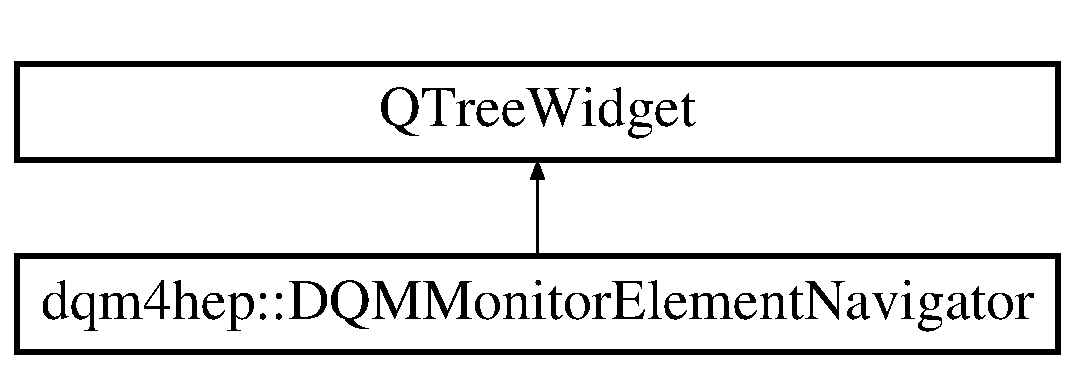
\includegraphics[height=2.000000cm]{classdqm4hep_1_1DQMMonitorElementNavigator}
\end{center}
\end{figure}
\subsection*{Public Types}
\begin{DoxyCompactItemize}
\item 
enum {\bf Item\+Type} \{ {\bf D\+I\+R\+E\+C\+T\+O\+R\+Y\+\_\+\+I\+T\+E\+M} = 1, 
{\bf M\+O\+N\+I\+T\+O\+R\+\_\+\+E\+L\+E\+M\+E\+N\+T\+\_\+\+I\+T\+E\+M} = 2
 \}
\begin{DoxyCompactList}\small\item\em Item\+Type enumerator. \end{DoxyCompactList}\end{DoxyCompactItemize}
\subsection*{Public Slots}
\begin{DoxyCompactItemize}
\item 
void {\bf check\+All\+Monitor\+Elements} ()
\begin{DoxyCompactList}\small\item\em Check all monitor element items. \end{DoxyCompactList}\item 
void {\bf uncheck\+All\+Monitor\+Elements} ()
\begin{DoxyCompactList}\small\item\em Uncheck all monitor element items. \end{DoxyCompactList}\item 
void {\bf check\+Selected\+Monitor\+Elements} ()
\begin{DoxyCompactList}\small\item\em Check selected monitor element items. \end{DoxyCompactList}\item 
void {\bf uncheck\+Selected\+Monitor\+Elements} ()
\begin{DoxyCompactList}\small\item\em Uncheck selected monitor element items. \end{DoxyCompactList}\end{DoxyCompactItemize}
\subsection*{Public Member Functions}
\begin{DoxyCompactItemize}
\item 
{\bf D\+Q\+M\+Monitor\+Element\+Navigator} (const Q\+String \&collector\+Name, {\bf D\+Q\+M\+Monitoring} $\ast$p\+Monitoring, Q\+Widget $\ast$p\+Parent=0)
\begin{DoxyCompactList}\small\item\em Constructor. \end{DoxyCompactList}\item 
{\bf $\sim$\+D\+Q\+M\+Monitor\+Element\+Navigator} ()
\begin{DoxyCompactList}\small\item\em Destructor. \end{DoxyCompactList}\item 
{\bf D\+Q\+M\+Monitoring} $\ast$ {\bf get\+Monitoring} () const 
\begin{DoxyCompactList}\small\item\em Get the monitoring instance. \end{DoxyCompactList}\item 
const Q\+String \& {\bf get\+Collector\+Name} () const 
\begin{DoxyCompactList}\small\item\em Get the collector name. \end{DoxyCompactList}\item 
Q\+String\+List {\bf get\+Module\+Names} () const 
\begin{DoxyCompactList}\small\item\em Get the module name list. \end{DoxyCompactList}\item 
Q\+Tree\+Widget\+Item $\ast$ {\bf mkdir} (const Q\+String \&module\+Name)
\begin{DoxyCompactList}\small\item\em Create a directory and return the directory. \end{DoxyCompactList}\item 
Q\+Tree\+Widget\+Item $\ast$ {\bf mkdir} (const Q\+String \&module\+Name, const Q\+String \&full\+Path\+Dir\+Name)
\begin{DoxyCompactList}\small\item\em Create a directory and return the directory. \end{DoxyCompactList}\item 
bool {\bf rmdir} (const Q\+String \&module\+Name)
\begin{DoxyCompactList}\small\item\em Remove the directory. \end{DoxyCompactList}\item 
bool {\bf rmdir} (const Q\+String \&module\+Name, const Q\+String \&full\+Path\+Dir\+Name)
\begin{DoxyCompactList}\small\item\em Remove the directory. \end{DoxyCompactList}\item 
bool {\bf dir\+Exists} (const Q\+String \&module\+Name)
\begin{DoxyCompactList}\small\item\em Whether the directory exists. \end{DoxyCompactList}\item 
bool {\bf dir\+Exists} (const Q\+String \&module\+Name, const Q\+String \&full\+Path\+Dir\+Name)
\begin{DoxyCompactList}\small\item\em Whether the directory exists. \end{DoxyCompactList}\item 
void {\bf clear} ()
\begin{DoxyCompactList}\small\item\em Clear the tree structure. \end{DoxyCompactList}\item 
void {\bf update\+Monitor\+Element} ({\bf D\+Q\+M\+Gui\+Monitor\+Element} $\ast$p\+Monitor\+Element)
\begin{DoxyCompactList}\small\item\em Create an entry (if doesn't exists) from the monitor element. \end{DoxyCompactList}\item 
void {\bf update\+Monitor\+Elements} (const {\bf D\+Q\+M\+Gui\+Monitor\+Element\+List} \&monitor\+Element\+List)
\begin{DoxyCompactList}\small\item\em Create an entry (if doesn't exists) for each of the monitor elements. \end{DoxyCompactList}\item 
void {\bf remove\+Monitor\+Element} ({\bf D\+Q\+M\+Gui\+Monitor\+Element} $\ast$p\+Monitor\+Element)
\begin{DoxyCompactList}\small\item\em Remove the monitor element from the tree widget. \end{DoxyCompactList}\item 
Q\+Tree\+Widget\+Item $\ast$ {\bf add\+Monitor\+Element} (Q\+Tree\+Widget\+Item $\ast$p\+Tree\+Item, const Q\+String \&name)
\begin{DoxyCompactList}\small\item\em Add a monitor element item and set p\+Tree\+Item as its parent item. \end{DoxyCompactList}\item 
Q\+String {\bf get\+Full\+Path\+Name} (Q\+Tree\+Widget\+Item $\ast$p\+Tree\+Item) const 
\begin{DoxyCompactList}\small\item\em Get the full path name of the tree item. \end{DoxyCompactList}\item 
Q\+String {\bf get\+Module\+Name} (Q\+Tree\+Widget\+Item $\ast$p\+Tree\+Item) const 
\begin{DoxyCompactList}\small\item\em Get the module name of the tree item. \end{DoxyCompactList}\item 
bool {\bf is\+Directory\+Item} (Q\+Tree\+Widget\+Item $\ast$p\+Tree\+Item) const 
\begin{DoxyCompactList}\small\item\em Whether the tree item is a directory. \end{DoxyCompactList}\item 
bool {\bf is\+Monitor\+Element\+Item} (Q\+Tree\+Widget\+Item $\ast$p\+Tree\+Item) const 
\begin{DoxyCompactList}\small\item\em Whether the tree item is a monitor element item. \end{DoxyCompactList}\item 
Q\+List$<$ Q\+Tree\+Widget\+Item $\ast$ $>$ {\bf get\+Selected\+Monitor\+Element\+Items} () const 
\begin{DoxyCompactList}\small\item\em Get the selected monitor element items. \end{DoxyCompactList}\item 
Q\+List$<$ Q\+Tree\+Widget\+Item $\ast$ $>$ {\bf get\+Selected\+Directory\+Items} () const 
\begin{DoxyCompactList}\small\item\em Get the selected directory items. \end{DoxyCompactList}\item 
Q\+List$<$ Q\+Tree\+Widget\+Item $\ast$ $>$ {\bf get\+Checked\+Monitor\+Elements} () const 
\begin{DoxyCompactList}\small\item\em Get the checked monitor element items. \end{DoxyCompactList}\item 
Q\+List$<$ Q\+Tree\+Widget\+Item $\ast$ $>$ {\bf get\+All\+Monitor\+Element\+Items} (const Q\+String \&module\+Name) const 
\begin{DoxyCompactList}\small\item\em Get all monitor element items for a given module. \end{DoxyCompactList}\item 
void {\bf enable\+Subscription} (bool enable=true)
\begin{DoxyCompactList}\small\item\em Enable/\+Disable subscription for each element. \end{DoxyCompactList}\end{DoxyCompactItemize}
\subsection*{Private Slots}
\begin{DoxyCompactItemize}
\item 
void {\bf show\+Context\+Menu} (const Q\+Point \&point)
\item 
void {\bf draw\+Selected\+Monitor\+Elements} ()
\item 
void {\bf handle\+Item\+Double\+Click} (Q\+Tree\+Widget\+Item $\ast$p\+Tree\+Widget\+Item, int column)
\item 
void {\bf handle\+Item\+Expanded} (Q\+Tree\+Widget\+Item $\ast$p\+Tree\+Widget\+Item)
\item 
void {\bf handle\+Item\+Collapsed} (Q\+Tree\+Widget\+Item $\ast$p\+Tree\+Widget\+Item)
\item 
void {\bf start\+Drag} ()
\item 
void {\bf query\+Update} ()
\end{DoxyCompactItemize}
\subsection*{Private Member Functions}
\begin{DoxyCompactItemize}
\item 
Q\+Tree\+Widget\+Item $\ast$ {\bf mkdir} (Q\+Tree\+Widget\+Item $\ast$p\+Tree\+Item, const Q\+String \&dir\+Name)
\begin{DoxyCompactList}\small\item\em Create a directory and set p\+Tree\+Item as parent item. \end{DoxyCompactList}\item 
bool {\bf dir\+Exists} (Q\+Tree\+Widget\+Item $\ast$p\+Tree\+Item, const Q\+String \&name) const 
\item 
void {\bf clear} (Q\+Tree\+Widget\+Item $\ast$p\+Tree\+Item) const 
\item 
void {\bf get\+Recursive\+Monitor\+Elements} (Q\+Tree\+Widget\+Item $\ast$p\+Tree\+Item, Q\+List$<$ Q\+Tree\+Widget\+Item $\ast$ $>$ \&monitor\+Element\+Items, bool only\+Checked=false) const 
\item 
void {\bf key\+Press\+Event} (Q\+Key\+Event $\ast$p\+Key\+Event)
\item 
void {\bf mouse\+Press\+Event} (Q\+Mouse\+Event $\ast$p\+Mouse\+Event)
\end{DoxyCompactItemize}
\subsection*{Private Attributes}
\begin{DoxyCompactItemize}
\item 
{\bf D\+Q\+M\+Monitoring} $\ast$ {\bf m\+\_\+p\+Monitoring}
\item 
Q\+String {\bf m\+\_\+collector\+Name}
\item 
Q\+List$<$ Q\+Tree\+Widget\+Item $\ast$ $>$ {\bf m\+\_\+drag\+Item\+List}
\item 
bool {\bf m\+\_\+subscription\+Enabled}
\end{DoxyCompactItemize}


\subsection{Detailed Description}
\doxyref{D\+Q\+M\+Monitor\+Element\+Navigator}{p.}{classdqm4hep_1_1DQMMonitorElementNavigator} class. 

Definition at line 47 of file D\+Q\+M\+Monitor\+Element\+View.\+h.



\subsection{Member Enumeration Documentation}
\index{dqm4hep\+::\+D\+Q\+M\+Monitor\+Element\+Navigator@{dqm4hep\+::\+D\+Q\+M\+Monitor\+Element\+Navigator}!Item\+Type@{Item\+Type}}
\index{Item\+Type@{Item\+Type}!dqm4hep\+::\+D\+Q\+M\+Monitor\+Element\+Navigator@{dqm4hep\+::\+D\+Q\+M\+Monitor\+Element\+Navigator}}
\subsubsection[{Item\+Type}]{\setlength{\rightskip}{0pt plus 5cm}enum {\bf dqm4hep\+::\+D\+Q\+M\+Monitor\+Element\+Navigator\+::\+Item\+Type}}\label{classdqm4hep_1_1DQMMonitorElementNavigator_a2239041d57cac730db21661763c74be7}


Item\+Type enumerator. 

\begin{Desc}
\item[Enumerator]\par
\begin{description}
\index{D\+I\+R\+E\+C\+T\+O\+R\+Y\+\_\+\+I\+T\+E\+M@{D\+I\+R\+E\+C\+T\+O\+R\+Y\+\_\+\+I\+T\+E\+M}!dqm4hep\+::\+D\+Q\+M\+Monitor\+Element\+Navigator@{dqm4hep\+::\+D\+Q\+M\+Monitor\+Element\+Navigator}}\index{dqm4hep\+::\+D\+Q\+M\+Monitor\+Element\+Navigator@{dqm4hep\+::\+D\+Q\+M\+Monitor\+Element\+Navigator}!D\+I\+R\+E\+C\+T\+O\+R\+Y\+\_\+\+I\+T\+E\+M@{D\+I\+R\+E\+C\+T\+O\+R\+Y\+\_\+\+I\+T\+E\+M}}\item[{\em 
D\+I\+R\+E\+C\+T\+O\+R\+Y\+\_\+\+I\+T\+E\+M\label{classdqm4hep_1_1DQMMonitorElementNavigator_a2239041d57cac730db21661763c74be7afe9683b2c432d1c68d2dc431709675d7}
}]\index{M\+O\+N\+I\+T\+O\+R\+\_\+\+E\+L\+E\+M\+E\+N\+T\+\_\+\+I\+T\+E\+M@{M\+O\+N\+I\+T\+O\+R\+\_\+\+E\+L\+E\+M\+E\+N\+T\+\_\+\+I\+T\+E\+M}!dqm4hep\+::\+D\+Q\+M\+Monitor\+Element\+Navigator@{dqm4hep\+::\+D\+Q\+M\+Monitor\+Element\+Navigator}}\index{dqm4hep\+::\+D\+Q\+M\+Monitor\+Element\+Navigator@{dqm4hep\+::\+D\+Q\+M\+Monitor\+Element\+Navigator}!M\+O\+N\+I\+T\+O\+R\+\_\+\+E\+L\+E\+M\+E\+N\+T\+\_\+\+I\+T\+E\+M@{M\+O\+N\+I\+T\+O\+R\+\_\+\+E\+L\+E\+M\+E\+N\+T\+\_\+\+I\+T\+E\+M}}\item[{\em 
M\+O\+N\+I\+T\+O\+R\+\_\+\+E\+L\+E\+M\+E\+N\+T\+\_\+\+I\+T\+E\+M\label{classdqm4hep_1_1DQMMonitorElementNavigator_a2239041d57cac730db21661763c74be7a31a680d43dc2194b1e9263f1d767f98b}
}]\end{description}
\end{Desc}


Definition at line 54 of file D\+Q\+M\+Monitor\+Element\+View.\+h.


\begin{DoxyCode}
55   \{
56     DIRECTORY_ITEM = 1,
57     MONITOR_ELEMENT_ITEM = 2
58   \};
\end{DoxyCode}


\subsection{Constructor \& Destructor Documentation}
\index{dqm4hep\+::\+D\+Q\+M\+Monitor\+Element\+Navigator@{dqm4hep\+::\+D\+Q\+M\+Monitor\+Element\+Navigator}!D\+Q\+M\+Monitor\+Element\+Navigator@{D\+Q\+M\+Monitor\+Element\+Navigator}}
\index{D\+Q\+M\+Monitor\+Element\+Navigator@{D\+Q\+M\+Monitor\+Element\+Navigator}!dqm4hep\+::\+D\+Q\+M\+Monitor\+Element\+Navigator@{dqm4hep\+::\+D\+Q\+M\+Monitor\+Element\+Navigator}}
\subsubsection[{D\+Q\+M\+Monitor\+Element\+Navigator}]{\setlength{\rightskip}{0pt plus 5cm}dqm4hep\+::\+D\+Q\+M\+Monitor\+Element\+Navigator\+::\+D\+Q\+M\+Monitor\+Element\+Navigator (
\begin{DoxyParamCaption}
\item[{const Q\+String \&}]{collector\+Name, }
\item[{{\bf D\+Q\+M\+Monitoring} $\ast$}]{p\+Monitoring, }
\item[{Q\+Widget $\ast$}]{p\+Parent = {\ttfamily 0}}
\end{DoxyParamCaption}
)}\label{classdqm4hep_1_1DQMMonitorElementNavigator_aaa989c7120cf0de6dc3e0d3943925973}


Constructor. 



Definition at line 177 of file D\+Q\+M\+Monitor\+Element\+View.\+cc.



References handle\+Item\+Collapsed(), handle\+Item\+Double\+Click(), handle\+Item\+Expanded(), and show\+Context\+Menu().


\begin{DoxyCode}
177                                                                                                            
                            :
178     m_collectorName(collectorName),
179     QTreeWidget(pParent),
180     m_pMonitoring(pMonitoring),
181     m_subscriptionEnabled(\textcolor{keyword}{true})
182 \{
183   setHeaderLabel(\textcolor{stringliteral}{"Monitor elements"});
184 
185   setContextMenuPolicy(Qt::CustomContextMenu);
186   setSelectionMode(QAbstractItemView::ExtendedSelection);
187   setSelectionBehavior(QAbstractItemView::SelectRows);
188 
189   setFocusPolicy(Qt::StrongFocus);
190 
191   connect(\textcolor{keyword}{this}, SIGNAL(customContextMenuRequested(\textcolor{keyword}{const} QPoint &)),
192       \textcolor{keyword}{this}, SLOT(showContextMenu(\textcolor{keyword}{const} QPoint &)));
193 
194     connect(\textcolor{keyword}{this}, SIGNAL(itemDoubleClicked(QTreeWidgetItem *, \textcolor{keywordtype}{int})),
195             \textcolor{keyword}{this}, SLOT(handleItemDoubleClick(QTreeWidgetItem *, \textcolor{keywordtype}{int})));
196 
197     connect(\textcolor{keyword}{this}, SIGNAL(itemExpanded(QTreeWidgetItem *)),
198         \textcolor{keyword}{this}, SLOT(handleItemExpanded(QTreeWidgetItem *)));
199 
200     connect(\textcolor{keyword}{this}, SIGNAL(itemCollapsed(QTreeWidgetItem *)),
201         \textcolor{keyword}{this}, SLOT(handleItemCollapsed(QTreeWidgetItem *)));
202 \}
\end{DoxyCode}
\index{dqm4hep\+::\+D\+Q\+M\+Monitor\+Element\+Navigator@{dqm4hep\+::\+D\+Q\+M\+Monitor\+Element\+Navigator}!````~D\+Q\+M\+Monitor\+Element\+Navigator@{$\sim$\+D\+Q\+M\+Monitor\+Element\+Navigator}}
\index{````~D\+Q\+M\+Monitor\+Element\+Navigator@{$\sim$\+D\+Q\+M\+Monitor\+Element\+Navigator}!dqm4hep\+::\+D\+Q\+M\+Monitor\+Element\+Navigator@{dqm4hep\+::\+D\+Q\+M\+Monitor\+Element\+Navigator}}
\subsubsection[{$\sim$\+D\+Q\+M\+Monitor\+Element\+Navigator}]{\setlength{\rightskip}{0pt plus 5cm}dqm4hep\+::\+D\+Q\+M\+Monitor\+Element\+Navigator\+::$\sim$\+D\+Q\+M\+Monitor\+Element\+Navigator (
\begin{DoxyParamCaption}
{}
\end{DoxyParamCaption}
)}\label{classdqm4hep_1_1DQMMonitorElementNavigator_a61bcdfdf90a8f36c53dc891bdb9bdfac}


Destructor. 



Definition at line 206 of file D\+Q\+M\+Monitor\+Element\+View.\+cc.


\begin{DoxyCode}
207 \{
208   \textcolor{comment}{/* nop */}
209 \}
\end{DoxyCode}


\subsection{Member Function Documentation}
\index{dqm4hep\+::\+D\+Q\+M\+Monitor\+Element\+Navigator@{dqm4hep\+::\+D\+Q\+M\+Monitor\+Element\+Navigator}!add\+Monitor\+Element@{add\+Monitor\+Element}}
\index{add\+Monitor\+Element@{add\+Monitor\+Element}!dqm4hep\+::\+D\+Q\+M\+Monitor\+Element\+Navigator@{dqm4hep\+::\+D\+Q\+M\+Monitor\+Element\+Navigator}}
\subsubsection[{add\+Monitor\+Element}]{\setlength{\rightskip}{0pt plus 5cm}Q\+Tree\+Widget\+Item $\ast$ dqm4hep\+::\+D\+Q\+M\+Monitor\+Element\+Navigator\+::add\+Monitor\+Element (
\begin{DoxyParamCaption}
\item[{Q\+Tree\+Widget\+Item $\ast$}]{p\+Tree\+Item, }
\item[{const Q\+String \&}]{name}
\end{DoxyParamCaption}
)}\label{classdqm4hep_1_1DQMMonitorElementNavigator_a63dc948bfb013e5e928e3a647015491a}


Add a monitor element item and set p\+Tree\+Item as its parent item. 

If the monitor element item already exists in child items of p\+Tree\+Item, it is not created.

Returns the created/existing monitor element item 

Definition at line 711 of file D\+Q\+M\+Monitor\+Element\+View.\+cc.



References is\+Directory\+Item(), is\+Monitor\+Element\+Item(), m\+\_\+subscription\+Enabled, M\+O\+N\+I\+T\+O\+R\+\_\+\+E\+L\+E\+M\+E\+N\+T\+\_\+\+I\+T\+E\+M, dqm4hep\+::\+Tree\+Widget\+Item\+::set\+Checkable(), and dqm4hep\+::\+Tree\+Widget\+Item\+::set\+Data().



Referenced by dqm4hep\+::\+D\+Q\+M\+Monitor\+Element\+View\+::from\+Xml(), and update\+Monitor\+Element().


\begin{DoxyCode}
712 \{
713   \textcolor{keywordflow}{if}(!this->isDirectoryItem(pTreeItem))
714     \textcolor{keywordflow}{return} 0;
715 
716   \textcolor{keywordflow}{for}(\textcolor{keywordtype}{int} i=0 ; i<pTreeItem->childCount() ; i++)
717   \{
718     \textcolor{keywordflow}{if}(name == pTreeItem->child(i)->text(0) && this->isMonitorElementItem(pTreeItem->child(i)))
719       \textcolor{keywordflow}{return} pTreeItem->child(i);
720   \}
721 
722   TreeWidgetItem *pMonitorElementItem = \textcolor{keyword}{new} TreeWidgetItem(pTreeItem);
723   pMonitorElementItem->setText(0, name);
724   pMonitorElementItem->setData(0, Qt::UserRole, static\_cast<int>(
      MONITOR_ELEMENT_ITEM));
725   pMonitorElementItem->setCheckState(0, Qt::Unchecked);
726   pMonitorElementItem->setCheckable( m_subscriptionEnabled );
727   pTreeItem->addChild(pMonitorElementItem);
728 
729   \textcolor{keywordflow}{return} pMonitorElementItem;
730 \}
\end{DoxyCode}
\index{dqm4hep\+::\+D\+Q\+M\+Monitor\+Element\+Navigator@{dqm4hep\+::\+D\+Q\+M\+Monitor\+Element\+Navigator}!check\+All\+Monitor\+Elements@{check\+All\+Monitor\+Elements}}
\index{check\+All\+Monitor\+Elements@{check\+All\+Monitor\+Elements}!dqm4hep\+::\+D\+Q\+M\+Monitor\+Element\+Navigator@{dqm4hep\+::\+D\+Q\+M\+Monitor\+Element\+Navigator}}
\subsubsection[{check\+All\+Monitor\+Elements}]{\setlength{\rightskip}{0pt plus 5cm}void dqm4hep\+::\+D\+Q\+M\+Monitor\+Element\+Navigator\+::check\+All\+Monitor\+Elements (
\begin{DoxyParamCaption}
{}
\end{DoxyParamCaption}
)\hspace{0.3cm}{\ttfamily [slot]}}\label{classdqm4hep_1_1DQMMonitorElementNavigator_a4d55f833e869cb821dcbd4a12c895435}


Check all monitor element items. 



Definition at line 592 of file D\+Q\+M\+Monitor\+Element\+View.\+cc.



References get\+Recursive\+Monitor\+Elements().



Referenced by show\+Context\+Menu().


\begin{DoxyCode}
593 \{
594   \textcolor{keywordflow}{for}(\textcolor{keywordtype}{int} i=0 ; i<topLevelItemCount() ; i++)
595   \{
596     QTreeWidgetItem *pModuleItem = topLevelItem(i);
597 
598     QList<QTreeWidgetItem*> uncheckedMonitorElements;
599     this->getRecursiveMonitorElements(pModuleItem, uncheckedMonitorElements, \textcolor{keyword}{false});
600 
601     \textcolor{keywordflow}{for}(\textcolor{keywordtype}{int} j=0 ; j<uncheckedMonitorElements.count() ; j++)
602       uncheckedMonitorElements.at(j)->setCheckState(0, Qt::Checked);
603   \}
604 \}
\end{DoxyCode}
\index{dqm4hep\+::\+D\+Q\+M\+Monitor\+Element\+Navigator@{dqm4hep\+::\+D\+Q\+M\+Monitor\+Element\+Navigator}!check\+Selected\+Monitor\+Elements@{check\+Selected\+Monitor\+Elements}}
\index{check\+Selected\+Monitor\+Elements@{check\+Selected\+Monitor\+Elements}!dqm4hep\+::\+D\+Q\+M\+Monitor\+Element\+Navigator@{dqm4hep\+::\+D\+Q\+M\+Monitor\+Element\+Navigator}}
\subsubsection[{check\+Selected\+Monitor\+Elements}]{\setlength{\rightskip}{0pt plus 5cm}void dqm4hep\+::\+D\+Q\+M\+Monitor\+Element\+Navigator\+::check\+Selected\+Monitor\+Elements (
\begin{DoxyParamCaption}
{}
\end{DoxyParamCaption}
)\hspace{0.3cm}{\ttfamily [slot]}}\label{classdqm4hep_1_1DQMMonitorElementNavigator_a0cb3725039e6b8245feedc9a54901e66}


Check selected monitor element items. 



Definition at line 624 of file D\+Q\+M\+Monitor\+Element\+View.\+cc.



References get\+Recursive\+Monitor\+Elements(), and is\+Directory\+Item().



Referenced by show\+Context\+Menu().


\begin{DoxyCode}
625 \{
626   \textcolor{comment}{// Handle selected items instead of only the current item}
627   QList<QTreeWidgetItem *> selectedItems = this->selectedItems();
628   QSet<QTreeWidgetItem *> monitorElementItems;
629 
630   \textcolor{comment}{// first, get all monitor elements}
631   \textcolor{keywordflow}{for}(\textcolor{keywordtype}{int} i = 0; i < selectedItems.count(); i++)
632   \{
633     QTreeWidgetItem *pTreeWidgetItem = selectedItems.at(i);
634 
635     \textcolor{keywordflow}{if}(this->isDirectoryItem(pTreeWidgetItem))
636     \{
637       QList<QTreeWidgetItem *> monitorElementItemList;
638       this->getRecursiveMonitorElements(pTreeWidgetItem, monitorElementItemList, \textcolor{keyword}{false});
639       monitorElementItems += QSet<QTreeWidgetItem *>::fromList(monitorElementItemList);
640     \}
641     \textcolor{keywordflow}{else}
642       monitorElementItems << pTreeWidgetItem;
643   \}
644 
645   QSet<QTreeWidgetItem*>::iterator iter = monitorElementItems.begin();
646 
647   \textcolor{keywordflow}{while}(iter != monitorElementItems.end())
648   \{
649     QTreeWidgetItem *pTreeWidgetItem = *iter;
650     pTreeWidgetItem->setCheckState(0, Qt::Checked);
651     ++iter;
652   \}
653 \}
\end{DoxyCode}
\index{dqm4hep\+::\+D\+Q\+M\+Monitor\+Element\+Navigator@{dqm4hep\+::\+D\+Q\+M\+Monitor\+Element\+Navigator}!clear@{clear}}
\index{clear@{clear}!dqm4hep\+::\+D\+Q\+M\+Monitor\+Element\+Navigator@{dqm4hep\+::\+D\+Q\+M\+Monitor\+Element\+Navigator}}
\subsubsection[{clear}]{\setlength{\rightskip}{0pt plus 5cm}void dqm4hep\+::\+D\+Q\+M\+Monitor\+Element\+Navigator\+::clear (
\begin{DoxyParamCaption}
{}
\end{DoxyParamCaption}
)}\label{classdqm4hep_1_1DQMMonitorElementNavigator_ac0020f4216f6bac1dfe8e70302b77872}


Clear the tree structure. 



Definition at line 371 of file D\+Q\+M\+Monitor\+Element\+View.\+cc.



Referenced by clear(), dqm4hep\+::\+D\+Q\+M\+Monitor\+Element\+View\+::clear(), and rmdir().


\begin{DoxyCode}
372 \{
373   \textcolor{keywordflow}{while}(this->topLevelItemCount() != 0)
374   \{
375     QTreeWidgetItem *pTopLevelItem = this->topLevelItem(0);
376 
377     this->clear(pTopLevelItem);
378 
379     \textcolor{keyword}{delete} this->takeTopLevelItem(0);
380   \}
381 \}
\end{DoxyCode}
\index{dqm4hep\+::\+D\+Q\+M\+Monitor\+Element\+Navigator@{dqm4hep\+::\+D\+Q\+M\+Monitor\+Element\+Navigator}!clear@{clear}}
\index{clear@{clear}!dqm4hep\+::\+D\+Q\+M\+Monitor\+Element\+Navigator@{dqm4hep\+::\+D\+Q\+M\+Monitor\+Element\+Navigator}}
\subsubsection[{clear}]{\setlength{\rightskip}{0pt plus 5cm}void dqm4hep\+::\+D\+Q\+M\+Monitor\+Element\+Navigator\+::clear (
\begin{DoxyParamCaption}
\item[{Q\+Tree\+Widget\+Item $\ast$}]{p\+Tree\+Item}
\end{DoxyParamCaption}
) const\hspace{0.3cm}{\ttfamily [private]}}\label{classdqm4hep_1_1DQMMonitorElementNavigator_a00a47d85bea968e91f44319c52000648}


Definition at line 747 of file D\+Q\+M\+Monitor\+Element\+View.\+cc.



References clear().


\begin{DoxyCode}
748 \{
749   NOTIFY\_METHOD\_CALLED
750 
751   \textcolor{keywordflow}{while}(pTreeItem->childCount() != 0)
752   \{
753     QTreeWidgetItem *pChildItem = pTreeItem->child(0);
754 
755     this->clear(pChildItem);
756 
757     pTreeItem->removeChild(0);
758     \textcolor{keyword}{delete} pChildItem;
759   \}
760 \}
\end{DoxyCode}
\index{dqm4hep\+::\+D\+Q\+M\+Monitor\+Element\+Navigator@{dqm4hep\+::\+D\+Q\+M\+Monitor\+Element\+Navigator}!dir\+Exists@{dir\+Exists}}
\index{dir\+Exists@{dir\+Exists}!dqm4hep\+::\+D\+Q\+M\+Monitor\+Element\+Navigator@{dqm4hep\+::\+D\+Q\+M\+Monitor\+Element\+Navigator}}
\subsubsection[{dir\+Exists}]{\setlength{\rightskip}{0pt plus 5cm}bool dqm4hep\+::\+D\+Q\+M\+Monitor\+Element\+Navigator\+::dir\+Exists (
\begin{DoxyParamCaption}
\item[{const Q\+String \&}]{module\+Name}
\end{DoxyParamCaption}
)}\label{classdqm4hep_1_1DQMMonitorElementNavigator_aa766cad742ca5beecb6ba670daaf2736}


Whether the directory exists. 



Definition at line 318 of file D\+Q\+M\+Monitor\+Element\+View.\+cc.



Referenced by dir\+Exists(), remove\+Monitor\+Element(), and rmdir().


\begin{DoxyCode}
319 \{
320   QTreeWidgetItem *pModuleDirectoryItem = NULL;
321 
322   \textcolor{keywordflow}{for}(\textcolor{keywordtype}{int} i=0 ; i<topLevelItemCount() ; i++)
323   \{
324     \textcolor{keywordflow}{if}(moduleName == this->topLevelItem(i)->text(0))
325     \{
326       pModuleDirectoryItem = this->topLevelItem(i);
327       \textcolor{keywordflow}{break};
328     \}
329   \}
330 
331   \textcolor{keywordflow}{return} (NULL != pModuleDirectoryItem);
332 \}
\end{DoxyCode}
\index{dqm4hep\+::\+D\+Q\+M\+Monitor\+Element\+Navigator@{dqm4hep\+::\+D\+Q\+M\+Monitor\+Element\+Navigator}!dir\+Exists@{dir\+Exists}}
\index{dir\+Exists@{dir\+Exists}!dqm4hep\+::\+D\+Q\+M\+Monitor\+Element\+Navigator@{dqm4hep\+::\+D\+Q\+M\+Monitor\+Element\+Navigator}}
\subsubsection[{dir\+Exists}]{\setlength{\rightskip}{0pt plus 5cm}bool dqm4hep\+::\+D\+Q\+M\+Monitor\+Element\+Navigator\+::dir\+Exists (
\begin{DoxyParamCaption}
\item[{const Q\+String \&}]{module\+Name, }
\item[{const Q\+String \&}]{full\+Path\+Dir\+Name}
\end{DoxyParamCaption}
)}\label{classdqm4hep_1_1DQMMonitorElementNavigator_a4f05100c3a4837123bccbc6f4cf2cae7}


Whether the directory exists. 



Definition at line 336 of file D\+Q\+M\+Monitor\+Element\+View.\+cc.



References dir\+Exists(), and mkdir().


\begin{DoxyCode}
337 \{
338   QTreeWidgetItem *pModuleDirectoryItem = NULL;
339 
340   \textcolor{keywordflow}{for}(\textcolor{keywordtype}{int} i=0 ; i<topLevelItemCount() ; i++)
341   \{
342     \textcolor{keywordflow}{if}(moduleName == this->topLevelItem(i)->text(0))
343     \{
344       pModuleDirectoryItem = this->topLevelItem(i);
345       \textcolor{keywordflow}{break};
346     \}
347   \}
348 
349   \textcolor{keywordflow}{if}(NULL == pModuleDirectoryItem)
350     \textcolor{keywordflow}{return} \textcolor{keyword}{false};
351 
352   std::string path = fullPathDirName.toStdString();
353   std::vector<std::string> tokens;
354   DQM4HEP::tokenize(path, tokens, \textcolor{stringliteral}{"/"});
355 
356   QTreeWidgetItem *pCurrentDirectory = pModuleDirectoryItem;
357 
358   \textcolor{keywordflow}{for}(\textcolor{keywordtype}{unsigned} \textcolor{keywordtype}{int} i=0 ; i<tokens.size() ; i++)
359   \{
360     \textcolor{keywordflow}{if}(this->dirExists(pCurrentDirectory, tokens.at(i).c\_str()))
361       pCurrentDirectory = this->mkdir(pCurrentDirectory, tokens.at(i).c\_str());
362     \textcolor{keywordflow}{else}
363       \textcolor{keywordflow}{return} \textcolor{keyword}{false};
364   \}
365 
366   \textcolor{keywordflow}{return} \textcolor{keyword}{true};
367 \}
\end{DoxyCode}
\index{dqm4hep\+::\+D\+Q\+M\+Monitor\+Element\+Navigator@{dqm4hep\+::\+D\+Q\+M\+Monitor\+Element\+Navigator}!dir\+Exists@{dir\+Exists}}
\index{dir\+Exists@{dir\+Exists}!dqm4hep\+::\+D\+Q\+M\+Monitor\+Element\+Navigator@{dqm4hep\+::\+D\+Q\+M\+Monitor\+Element\+Navigator}}
\subsubsection[{dir\+Exists}]{\setlength{\rightskip}{0pt plus 5cm}bool dqm4hep\+::\+D\+Q\+M\+Monitor\+Element\+Navigator\+::dir\+Exists (
\begin{DoxyParamCaption}
\item[{Q\+Tree\+Widget\+Item $\ast$}]{p\+Tree\+Item, }
\item[{const Q\+String \&}]{name}
\end{DoxyParamCaption}
) const\hspace{0.3cm}{\ttfamily [private]}}\label{classdqm4hep_1_1DQMMonitorElementNavigator_afac6b1b42990baaf97079f0f5707cab2}


Definition at line 734 of file D\+Q\+M\+Monitor\+Element\+View.\+cc.



References is\+Monitor\+Element\+Item().


\begin{DoxyCode}
735 \{
736   \textcolor{keywordflow}{for}(\textcolor{keywordtype}{int} i=0 ; i<pTreeItem->childCount() ; i++)
737   \{
738     \textcolor{keywordflow}{if}(name == pTreeItem->child(i)->text(0) && this->isMonitorElementItem(pTreeItem->child(i)))
739       \textcolor{keywordflow}{return} \textcolor{keyword}{true};
740   \}
741 
742   \textcolor{keywordflow}{return} \textcolor{keyword}{false};
743 \}
\end{DoxyCode}
\index{dqm4hep\+::\+D\+Q\+M\+Monitor\+Element\+Navigator@{dqm4hep\+::\+D\+Q\+M\+Monitor\+Element\+Navigator}!draw\+Selected\+Monitor\+Elements@{draw\+Selected\+Monitor\+Elements}}
\index{draw\+Selected\+Monitor\+Elements@{draw\+Selected\+Monitor\+Elements}!dqm4hep\+::\+D\+Q\+M\+Monitor\+Element\+Navigator@{dqm4hep\+::\+D\+Q\+M\+Monitor\+Element\+Navigator}}
\subsubsection[{draw\+Selected\+Monitor\+Elements}]{\setlength{\rightskip}{0pt plus 5cm}void dqm4hep\+::\+D\+Q\+M\+Monitor\+Element\+Navigator\+::draw\+Selected\+Monitor\+Elements (
\begin{DoxyParamCaption}
{}
\end{DoxyParamCaption}
)\hspace{0.3cm}{\ttfamily [private]}, {\ttfamily [slot]}}\label{classdqm4hep_1_1DQMMonitorElementNavigator_aa39af7272e3350a9b1caf6be16386aad}


Definition at line 842 of file D\+Q\+M\+Monitor\+Element\+View.\+cc.



References dqm4hep\+::\+D\+Q\+M\+Canvas\+View\+::canvas\+Area\+Count(), dqm4hep\+::\+D\+Q\+M\+Canvas\+View\+::create\+Canvas\+Area\+And\+Set\+Current(), dqm4hep\+::\+D\+Q\+M\+Canvas\+View\+::draw\+In\+Area(), dqm4hep\+::\+D\+Q\+M\+Monitoring\+Model\+::find\+Monitor\+Element(), dqm4hep\+::\+D\+Q\+M\+Monitoring\+View\+::get\+Canvas\+View(), get\+Collector\+Name(), dqm4hep\+::\+D\+Q\+M\+Monitoring\+::get\+Controller(), get\+Full\+Path\+Name(), dqm4hep\+::\+D\+Q\+M\+Monitoring\+::get\+Model(), get\+Module\+Name(), get\+Monitoring(), get\+Selected\+Monitor\+Element\+Items(), dqm4hep\+::\+D\+Q\+M\+Monitoring\+::get\+View(), and dqm4hep\+::\+D\+Q\+M\+Monitoring\+Controller\+::log().



Referenced by show\+Context\+Menu().


\begin{DoxyCode}
843 \{
844   QAction *pAction = qobject\_cast<QAction*>(sender());
845 
846   \textcolor{keywordflow}{if}(!pAction)
847     \textcolor{keywordflow}{return};
848 
849   \textcolor{keywordtype}{int} areaIndex = pAction->data().toInt();
850   QList<QTreeWidgetItem*> selectedMonitorElements(this->
      getSelectedMonitorElementItems());
851   DQMCanvasView *pCanvasView = this->getMonitoring()->getView()->getCanvasView();
852 
853   \textcolor{keywordflow}{if}(areaIndex < 0)
854   \{
855     pCanvasView->createCanvasAreaAndSetCurrent();
856     areaIndex = pCanvasView->canvasAreaCount()-1;
857   \}
858 
859   \textcolor{keywordflow}{if}(areaIndex > pCanvasView->canvasAreaCount()-1)
860   \{
861     this->getMonitoring()->getController()->log(ERROR, QString(\textcolor{stringliteral}{"Canvas area not found ! (index = %1)"}).arg(
      areaIndex).toStdString());
862     \textcolor{keywordflow}{return};
863   \}
864 
865   \textcolor{keywordtype}{int} nDrawElements = 0;
866 
867   \textcolor{keywordflow}{for}(\textcolor{keywordtype}{int} i=0 ; i<selectedMonitorElements.count() ; i++)
868   \{
869     QTreeWidgetItem *pMonitorElementItem = selectedMonitorElements.at(i);
870 
871     QString collectorName(this->getCollectorName());
872     QString moduleName(this->getModuleName(pMonitorElementItem));
873     QString fullPathName(this->getFullPathName(pMonitorElementItem));
874     QString monitorElementName(pMonitorElementItem->text(0));
875 
876     DQMGuiMonitorElement *pMonitorElement =
877         this->getMonitoring()->getModel()->findMonitorElement(
878             collectorName.toStdString(),
879             moduleName.toStdString(),
880             fullPathName.toStdString(),
881             monitorElementName.toStdString());
882 
883     \textcolor{keywordflow}{if}(!pMonitorElement)
884       \textcolor{keywordflow}{continue};
885 
886     pCanvasView->drawInArea(pMonitorElement, areaIndex);
887     nDrawElements++;
888   \}
889 
890   \textcolor{keywordflow}{if}(nDrawElements == selectedMonitorElements.count())
891   \{
892     this->getMonitoring()->getController()->log(MESSAGE, QString(\textcolor{stringliteral}{"Number of drawn monitor elements : %1"}).
      arg(nDrawElements).toStdString());
893   \}
894   \textcolor{keywordflow}{else} \textcolor{keywordflow}{if}(nDrawElements < selectedMonitorElements.count() && nDrawElements != 0)
895   \{
896     this->getMonitoring()->getController()->log(WARNING, QString(\textcolor{stringliteral}{"Monitor elements drawn (%1 success, %2
       failed)"}).arg(nDrawElements).arg(selectedMonitorElements.count()-nDrawElements).toStdString());
897   \}
898   \textcolor{keywordflow}{else}
899   \{
900     this->getMonitoring()->getController()->log(ERROR, QString(\textcolor{stringliteral}{"No monitor elements drawn ! (%1 requested)"}
      ).arg(selectedMonitorElements.count()).toStdString());
901   \}
902 \}
\end{DoxyCode}
\index{dqm4hep\+::\+D\+Q\+M\+Monitor\+Element\+Navigator@{dqm4hep\+::\+D\+Q\+M\+Monitor\+Element\+Navigator}!enable\+Subscription@{enable\+Subscription}}
\index{enable\+Subscription@{enable\+Subscription}!dqm4hep\+::\+D\+Q\+M\+Monitor\+Element\+Navigator@{dqm4hep\+::\+D\+Q\+M\+Monitor\+Element\+Navigator}}
\subsubsection[{enable\+Subscription}]{\setlength{\rightskip}{0pt plus 5cm}void dqm4hep\+::\+D\+Q\+M\+Monitor\+Element\+Navigator\+::enable\+Subscription (
\begin{DoxyParamCaption}
\item[{bool}]{enable = {\ttfamily true}}
\end{DoxyParamCaption}
)}\label{classdqm4hep_1_1DQMMonitorElementNavigator_a12cd3ed3d3c74c19de91e531aeaa7b64}


Enable/\+Disable subscription for each element. 



Definition at line 570 of file D\+Q\+M\+Monitor\+Element\+View.\+cc.



References get\+Recursive\+Monitor\+Elements(), m\+\_\+subscription\+Enabled, and dqm4hep\+::\+Tree\+Widget\+Item\+::set\+Checkable().



Referenced by dqm4hep\+::\+D\+Q\+M\+Monitor\+Element\+View\+::enable\+Subscription().


\begin{DoxyCode}
571 \{
572   \textcolor{keywordflow}{if}(m_subscriptionEnabled == enable)
573     \textcolor{keywordflow}{return};
574 
575   m_subscriptionEnabled = enable;
576 
577   \textcolor{keywordflow}{for}(\textcolor{keywordtype}{int} i=0 ; i<topLevelItemCount() ; i++)
578   \{
579     QList<QTreeWidgetItem*> monitorElementItems;
580     this->getRecursiveMonitorElements(this->topLevelItem(i), monitorElementItems, \textcolor{keyword}{false});
581 
582     \textcolor{keywordflow}{for}(\textcolor{keywordtype}{int} j=0 ; j<monitorElementItems.size() ; j++)
583     \{
584       TreeWidgetItem *pMonitorElementItem = \textcolor{keyword}{dynamic\_cast<}TreeWidgetItem *\textcolor{keyword}{>}(monitorElementItems.at(j));
585       pMonitorElementItem->setCheckable( m_subscriptionEnabled );
586     \}
587   \}
588 \}
\end{DoxyCode}
\index{dqm4hep\+::\+D\+Q\+M\+Monitor\+Element\+Navigator@{dqm4hep\+::\+D\+Q\+M\+Monitor\+Element\+Navigator}!get\+All\+Monitor\+Element\+Items@{get\+All\+Monitor\+Element\+Items}}
\index{get\+All\+Monitor\+Element\+Items@{get\+All\+Monitor\+Element\+Items}!dqm4hep\+::\+D\+Q\+M\+Monitor\+Element\+Navigator@{dqm4hep\+::\+D\+Q\+M\+Monitor\+Element\+Navigator}}
\subsubsection[{get\+All\+Monitor\+Element\+Items}]{\setlength{\rightskip}{0pt plus 5cm}Q\+List$<$ Q\+Tree\+Widget\+Item $\ast$ $>$ dqm4hep\+::\+D\+Q\+M\+Monitor\+Element\+Navigator\+::get\+All\+Monitor\+Element\+Items (
\begin{DoxyParamCaption}
\item[{const Q\+String \&}]{module\+Name}
\end{DoxyParamCaption}
) const}\label{classdqm4hep_1_1DQMMonitorElementNavigator_a5553c42745981661d47784421c1378fe}


Get all monitor element items for a given module. 



Definition at line 552 of file D\+Q\+M\+Monitor\+Element\+View.\+cc.



References get\+Recursive\+Monitor\+Elements().



Referenced by dqm4hep\+::\+D\+Q\+M\+Monitor\+Element\+View\+::to\+Xml().


\begin{DoxyCode}
553 \{
554   QList<QTreeWidgetItem*> monitorElementItems;
555 
556   \textcolor{keywordflow}{for}(\textcolor{keywordtype}{int} i=0 ; i<topLevelItemCount() ; i++)
557   \{
558     \textcolor{keywordflow}{if}(this->topLevelItem(i)->text(0) == moduleName)
559     \{
560       this->getRecursiveMonitorElements(this->topLevelItem(i), monitorElementItems, \textcolor{keyword}{false});
561       \textcolor{keywordflow}{break};
562     \}
563   \}
564 
565   \textcolor{keywordflow}{return} monitorElementItems;
566 \}
\end{DoxyCode}
\index{dqm4hep\+::\+D\+Q\+M\+Monitor\+Element\+Navigator@{dqm4hep\+::\+D\+Q\+M\+Monitor\+Element\+Navigator}!get\+Checked\+Monitor\+Elements@{get\+Checked\+Monitor\+Elements}}
\index{get\+Checked\+Monitor\+Elements@{get\+Checked\+Monitor\+Elements}!dqm4hep\+::\+D\+Q\+M\+Monitor\+Element\+Navigator@{dqm4hep\+::\+D\+Q\+M\+Monitor\+Element\+Navigator}}
\subsubsection[{get\+Checked\+Monitor\+Elements}]{\setlength{\rightskip}{0pt plus 5cm}Q\+List$<$ Q\+Tree\+Widget\+Item $\ast$ $>$ dqm4hep\+::\+D\+Q\+M\+Monitor\+Element\+Navigator\+::get\+Checked\+Monitor\+Elements (
\begin{DoxyParamCaption}
{}
\end{DoxyParamCaption}
) const}\label{classdqm4hep_1_1DQMMonitorElementNavigator_ae12ec420cf5d599b24e075aac61b8297}


Get the checked monitor element items. 



Definition at line 537 of file D\+Q\+M\+Monitor\+Element\+View.\+cc.



References get\+Recursive\+Monitor\+Elements().



Referenced by dqm4hep\+::\+D\+Q\+M\+Monitor\+Element\+View\+::get\+Checked\+Monitor\+Elements().


\begin{DoxyCode}
538 \{
539   QList<QTreeWidgetItem*> checkedMonitorElements;
540 
541   \textcolor{keywordflow}{for}(\textcolor{keywordtype}{int} i=0 ; i<topLevelItemCount() ; i++)
542   \{
543     QTreeWidgetItem *pModuleItem = topLevelItem(i);
544     this->getRecursiveMonitorElements(pModuleItem, checkedMonitorElements, \textcolor{keyword}{true});
545   \}
546 
547   \textcolor{keywordflow}{return} checkedMonitorElements;
548 \}
\end{DoxyCode}
\index{dqm4hep\+::\+D\+Q\+M\+Monitor\+Element\+Navigator@{dqm4hep\+::\+D\+Q\+M\+Monitor\+Element\+Navigator}!get\+Collector\+Name@{get\+Collector\+Name}}
\index{get\+Collector\+Name@{get\+Collector\+Name}!dqm4hep\+::\+D\+Q\+M\+Monitor\+Element\+Navigator@{dqm4hep\+::\+D\+Q\+M\+Monitor\+Element\+Navigator}}
\subsubsection[{get\+Collector\+Name}]{\setlength{\rightskip}{0pt plus 5cm}const Q\+String \& dqm4hep\+::\+D\+Q\+M\+Monitor\+Element\+Navigator\+::get\+Collector\+Name (
\begin{DoxyParamCaption}
{}
\end{DoxyParamCaption}
) const}\label{classdqm4hep_1_1DQMMonitorElementNavigator_aa409a9a818784bcf348c25ccb5f2b731}


Get the collector name. 



Definition at line 220 of file D\+Q\+M\+Monitor\+Element\+View.\+cc.



References m\+\_\+collector\+Name.



Referenced by draw\+Selected\+Monitor\+Elements(), handle\+Item\+Double\+Click(), key\+Press\+Event(), query\+Update(), dqm4hep\+::\+Tree\+Widget\+Item\+::set\+Data(), and start\+Drag().


\begin{DoxyCode}
221 \{
222   \textcolor{keywordflow}{return} m_collectorName;
223 \}
\end{DoxyCode}
\index{dqm4hep\+::\+D\+Q\+M\+Monitor\+Element\+Navigator@{dqm4hep\+::\+D\+Q\+M\+Monitor\+Element\+Navigator}!get\+Full\+Path\+Name@{get\+Full\+Path\+Name}}
\index{get\+Full\+Path\+Name@{get\+Full\+Path\+Name}!dqm4hep\+::\+D\+Q\+M\+Monitor\+Element\+Navigator@{dqm4hep\+::\+D\+Q\+M\+Monitor\+Element\+Navigator}}
\subsubsection[{get\+Full\+Path\+Name}]{\setlength{\rightskip}{0pt plus 5cm}Q\+String dqm4hep\+::\+D\+Q\+M\+Monitor\+Element\+Navigator\+::get\+Full\+Path\+Name (
\begin{DoxyParamCaption}
\item[{Q\+Tree\+Widget\+Item $\ast$}]{p\+Tree\+Item}
\end{DoxyParamCaption}
) const}\label{classdqm4hep_1_1DQMMonitorElementNavigator_aa313529ce3cf0621db165547f2af1da2}


Get the full path name of the tree item. 

Can be a monitor element item or a simple directory 

Definition at line 435 of file D\+Q\+M\+Monitor\+Element\+View.\+cc.



References is\+Monitor\+Element\+Item().



Referenced by draw\+Selected\+Monitor\+Elements(), handle\+Item\+Double\+Click(), dqm4hep\+::\+D\+Q\+M\+Monitoring\+Controller\+::handle\+Server\+Startup(), key\+Press\+Event(), query\+Update(), dqm4hep\+::\+Tree\+Widget\+Item\+::set\+Data(), start\+Drag(), and dqm4hep\+::\+D\+Q\+M\+Monitor\+Element\+View\+::to\+Xml().


\begin{DoxyCode}
436 \{
437   \textcolor{keywordflow}{if}(!pTreeItem)
438     \textcolor{keywordflow}{return} QString();
439 
440   \textcolor{comment}{//   "/mod/dir1/dir2"}
441   \textcolor{comment}{//   "/"}
442   \textcolor{comment}{//   "/mod"}
443 
444   QString fullPathName;
445   QTreeWidgetItem *pCurrentItem = pTreeItem;
446 
447   \textcolor{comment}{// do not put the me name in the full path}
448   \textcolor{keywordflow}{if}(this->isMonitorElementItem(pTreeItem))
449     pCurrentItem = pCurrentItem->parent();
450 
451   \textcolor{keywordflow}{while}(1)
452   \{
453     \textcolor{keywordtype}{bool} isTopLevelItem = (pCurrentItem->parent() == 0);
454 
455     \textcolor{keywordflow}{if}(isTopLevelItem)
456       \textcolor{keywordflow}{break};
457 
458     fullPathName = pCurrentItem->text(0) + \textcolor{stringliteral}{"/"} + fullPathName;
459     pCurrentItem = pCurrentItem->parent();
460   \}
461 
462   fullPathName = \textcolor{stringliteral}{"/"} + fullPathName;
463 
464   \textcolor{keywordflow}{return} fullPathName;
465 \}
\end{DoxyCode}
\index{dqm4hep\+::\+D\+Q\+M\+Monitor\+Element\+Navigator@{dqm4hep\+::\+D\+Q\+M\+Monitor\+Element\+Navigator}!get\+Module\+Name@{get\+Module\+Name}}
\index{get\+Module\+Name@{get\+Module\+Name}!dqm4hep\+::\+D\+Q\+M\+Monitor\+Element\+Navigator@{dqm4hep\+::\+D\+Q\+M\+Monitor\+Element\+Navigator}}
\subsubsection[{get\+Module\+Name}]{\setlength{\rightskip}{0pt plus 5cm}Q\+String dqm4hep\+::\+D\+Q\+M\+Monitor\+Element\+Navigator\+::get\+Module\+Name (
\begin{DoxyParamCaption}
\item[{Q\+Tree\+Widget\+Item $\ast$}]{p\+Tree\+Item}
\end{DoxyParamCaption}
) const}\label{classdqm4hep_1_1DQMMonitorElementNavigator_ad0273196241d119a212dc29c2008dc16}


Get the module name of the tree item. 



Definition at line 469 of file D\+Q\+M\+Monitor\+Element\+View.\+cc.



Referenced by draw\+Selected\+Monitor\+Elements(), handle\+Item\+Double\+Click(), dqm4hep\+::\+D\+Q\+M\+Monitoring\+Controller\+::handle\+Server\+Startup(), key\+Press\+Event(), query\+Update(), dqm4hep\+::\+Tree\+Widget\+Item\+::set\+Data(), and start\+Drag().


\begin{DoxyCode}
470 \{
471   \textcolor{keywordflow}{if}(!pTreeItem)
472     \textcolor{keywordflow}{return} QString();
473 
474   QTreeWidgetItem *pCurrentItem = pTreeItem;
475 
476   \textcolor{keywordflow}{while}(1)
477   \{
478     pCurrentItem = pCurrentItem->parent();
479 
480     \textcolor{keywordtype}{bool} isTopLevelItem = (pCurrentItem->parent() == 0);
481 
482     \textcolor{keywordflow}{if}(isTopLevelItem)
483       \textcolor{keywordflow}{break};
484   \}
485 
486   \textcolor{keywordflow}{return} pCurrentItem->text(0);
487 \}
\end{DoxyCode}
\index{dqm4hep\+::\+D\+Q\+M\+Monitor\+Element\+Navigator@{dqm4hep\+::\+D\+Q\+M\+Monitor\+Element\+Navigator}!get\+Module\+Names@{get\+Module\+Names}}
\index{get\+Module\+Names@{get\+Module\+Names}!dqm4hep\+::\+D\+Q\+M\+Monitor\+Element\+Navigator@{dqm4hep\+::\+D\+Q\+M\+Monitor\+Element\+Navigator}}
\subsubsection[{get\+Module\+Names}]{\setlength{\rightskip}{0pt plus 5cm}Q\+String\+List dqm4hep\+::\+D\+Q\+M\+Monitor\+Element\+Navigator\+::get\+Module\+Names (
\begin{DoxyParamCaption}
{}
\end{DoxyParamCaption}
) const}\label{classdqm4hep_1_1DQMMonitorElementNavigator_a977a0367a0394e900016b68c3ec7dec8}


Get the module name list. 



Definition at line 227 of file D\+Q\+M\+Monitor\+Element\+View.\+cc.



Referenced by dqm4hep\+::\+D\+Q\+M\+Monitor\+Element\+View\+::to\+Xml().


\begin{DoxyCode}
228 \{
229   QStringList moduleNameList;
230 
231   \textcolor{keywordflow}{for}(\textcolor{keywordtype}{int} i=0 ; i<topLevelItemCount() ; i++)
232     moduleNameList << this->topLevelItem(i)->text(0);
233 
234   \textcolor{keywordflow}{return} moduleNameList;
235 \}
\end{DoxyCode}
\index{dqm4hep\+::\+D\+Q\+M\+Monitor\+Element\+Navigator@{dqm4hep\+::\+D\+Q\+M\+Monitor\+Element\+Navigator}!get\+Monitoring@{get\+Monitoring}}
\index{get\+Monitoring@{get\+Monitoring}!dqm4hep\+::\+D\+Q\+M\+Monitor\+Element\+Navigator@{dqm4hep\+::\+D\+Q\+M\+Monitor\+Element\+Navigator}}
\subsubsection[{get\+Monitoring}]{\setlength{\rightskip}{0pt plus 5cm}{\bf D\+Q\+M\+Monitoring} $\ast$ dqm4hep\+::\+D\+Q\+M\+Monitor\+Element\+Navigator\+::get\+Monitoring (
\begin{DoxyParamCaption}
{}
\end{DoxyParamCaption}
) const}\label{classdqm4hep_1_1DQMMonitorElementNavigator_a6430502e5e91a8b157973ca7f4784977}


Get the monitoring instance. 



Definition at line 213 of file D\+Q\+M\+Monitor\+Element\+View.\+cc.



References m\+\_\+p\+Monitoring.



Referenced by draw\+Selected\+Monitor\+Elements(), handle\+Item\+Double\+Click(), key\+Press\+Event(), query\+Update(), dqm4hep\+::\+Tree\+Widget\+Item\+::set\+Data(), show\+Context\+Menu(), start\+Drag(), and update\+Monitor\+Element().


\begin{DoxyCode}
214 \{
215   \textcolor{keywordflow}{return} m_pMonitoring;
216 \}
\end{DoxyCode}
\index{dqm4hep\+::\+D\+Q\+M\+Monitor\+Element\+Navigator@{dqm4hep\+::\+D\+Q\+M\+Monitor\+Element\+Navigator}!get\+Recursive\+Monitor\+Elements@{get\+Recursive\+Monitor\+Elements}}
\index{get\+Recursive\+Monitor\+Elements@{get\+Recursive\+Monitor\+Elements}!dqm4hep\+::\+D\+Q\+M\+Monitor\+Element\+Navigator@{dqm4hep\+::\+D\+Q\+M\+Monitor\+Element\+Navigator}}
\subsubsection[{get\+Recursive\+Monitor\+Elements}]{\setlength{\rightskip}{0pt plus 5cm}void dqm4hep\+::\+D\+Q\+M\+Monitor\+Element\+Navigator\+::get\+Recursive\+Monitor\+Elements (
\begin{DoxyParamCaption}
\item[{Q\+Tree\+Widget\+Item $\ast$}]{p\+Tree\+Item, }
\item[{Q\+List$<$ Q\+Tree\+Widget\+Item $\ast$ $>$ \&}]{monitor\+Element\+Items, }
\item[{bool}]{only\+Checked = {\ttfamily false}}
\end{DoxyParamCaption}
) const\hspace{0.3cm}{\ttfamily [private]}}\label{classdqm4hep_1_1DQMMonitorElementNavigator_a1f05c4d7958d001c0ca847f070dceb66}


Definition at line 764 of file D\+Q\+M\+Monitor\+Element\+View.\+cc.



References is\+Directory\+Item(), and is\+Monitor\+Element\+Item().



Referenced by check\+All\+Monitor\+Elements(), check\+Selected\+Monitor\+Elements(), enable\+Subscription(), get\+All\+Monitor\+Element\+Items(), get\+Checked\+Monitor\+Elements(), key\+Press\+Event(), mouse\+Press\+Event(), uncheck\+All\+Monitor\+Elements(), and uncheck\+Selected\+Monitor\+Elements().


\begin{DoxyCode}
765 \{
766   \textcolor{keywordflow}{for}(\textcolor{keywordtype}{int} i=0 ; i<pTreeItem->childCount() ; i++)
767   \{
768     \textcolor{keywordflow}{if}(this->isMonitorElementItem(pTreeItem->child(i)))
769     \{
770       \textcolor{keywordflow}{if}(onlyChecked && pTreeItem->child(i)->checkState(0) != Qt::Checked)
771         \textcolor{keywordflow}{continue};
772 
773       monitorElementItems.append(pTreeItem->child(i));
774     \}
775     \textcolor{keywordflow}{else} \textcolor{keywordflow}{if}(this->isDirectoryItem(pTreeItem->child(i)))
776     \{
777       this->getRecursiveMonitorElements(pTreeItem->child(i), monitorElementItems, onlyChecked);
778     \}
779   \}
780 \}
\end{DoxyCode}
\index{dqm4hep\+::\+D\+Q\+M\+Monitor\+Element\+Navigator@{dqm4hep\+::\+D\+Q\+M\+Monitor\+Element\+Navigator}!get\+Selected\+Directory\+Items@{get\+Selected\+Directory\+Items}}
\index{get\+Selected\+Directory\+Items@{get\+Selected\+Directory\+Items}!dqm4hep\+::\+D\+Q\+M\+Monitor\+Element\+Navigator@{dqm4hep\+::\+D\+Q\+M\+Monitor\+Element\+Navigator}}
\subsubsection[{get\+Selected\+Directory\+Items}]{\setlength{\rightskip}{0pt plus 5cm}Q\+List$<$ Q\+Tree\+Widget\+Item $\ast$ $>$ dqm4hep\+::\+D\+Q\+M\+Monitor\+Element\+Navigator\+::get\+Selected\+Directory\+Items (
\begin{DoxyParamCaption}
{}
\end{DoxyParamCaption}
) const}\label{classdqm4hep_1_1DQMMonitorElementNavigator_a788a6bbeffa97763206323c6c9a2e52e}


Get the selected directory items. 



Definition at line 521 of file D\+Q\+M\+Monitor\+Element\+View.\+cc.



References is\+Directory\+Item().


\begin{DoxyCode}
522 \{
523   QList<QTreeWidgetItem*> selectedItems = this->selectedItems();
524   QList<QTreeWidgetItem*> selectedDirectoryItems;
525 
526   \textcolor{keywordflow}{for}(\textcolor{keywordtype}{int} i=0 ; i<selectedItems.count() ; i++)
527   \{
528     \textcolor{keywordflow}{if}(this->isDirectoryItem(selectedItems.at(i)))
529       selectedDirectoryItems.append(selectedItems.at(i));
530   \}
531 
532   \textcolor{keywordflow}{return} selectedDirectoryItems;
533 \}
\end{DoxyCode}
\index{dqm4hep\+::\+D\+Q\+M\+Monitor\+Element\+Navigator@{dqm4hep\+::\+D\+Q\+M\+Monitor\+Element\+Navigator}!get\+Selected\+Monitor\+Element\+Items@{get\+Selected\+Monitor\+Element\+Items}}
\index{get\+Selected\+Monitor\+Element\+Items@{get\+Selected\+Monitor\+Element\+Items}!dqm4hep\+::\+D\+Q\+M\+Monitor\+Element\+Navigator@{dqm4hep\+::\+D\+Q\+M\+Monitor\+Element\+Navigator}}
\subsubsection[{get\+Selected\+Monitor\+Element\+Items}]{\setlength{\rightskip}{0pt plus 5cm}Q\+List$<$ Q\+Tree\+Widget\+Item $\ast$ $>$ dqm4hep\+::\+D\+Q\+M\+Monitor\+Element\+Navigator\+::get\+Selected\+Monitor\+Element\+Items (
\begin{DoxyParamCaption}
{}
\end{DoxyParamCaption}
) const}\label{classdqm4hep_1_1DQMMonitorElementNavigator_a5faca4d2ce2b08b6b7b619fec16e63b4}


Get the selected monitor element items. 



Definition at line 505 of file D\+Q\+M\+Monitor\+Element\+View.\+cc.



References is\+Monitor\+Element\+Item().



Referenced by draw\+Selected\+Monitor\+Elements(), handle\+Item\+Double\+Click(), and query\+Update().


\begin{DoxyCode}
506 \{
507   QList<QTreeWidgetItem*> selectedItems = this->selectedItems();
508   QList<QTreeWidgetItem*> selectedMonitorElementItems;
509 
510   \textcolor{keywordflow}{for}(\textcolor{keywordtype}{int} i=0 ; i<selectedItems.count() ; i++)
511   \{
512     \textcolor{keywordflow}{if}(this->isMonitorElementItem(selectedItems.at(i)))
513       selectedMonitorElementItems.append(selectedItems.at(i));
514   \}
515 
516   \textcolor{keywordflow}{return} selectedMonitorElementItems;
517 \}
\end{DoxyCode}
\index{dqm4hep\+::\+D\+Q\+M\+Monitor\+Element\+Navigator@{dqm4hep\+::\+D\+Q\+M\+Monitor\+Element\+Navigator}!handle\+Item\+Collapsed@{handle\+Item\+Collapsed}}
\index{handle\+Item\+Collapsed@{handle\+Item\+Collapsed}!dqm4hep\+::\+D\+Q\+M\+Monitor\+Element\+Navigator@{dqm4hep\+::\+D\+Q\+M\+Monitor\+Element\+Navigator}}
\subsubsection[{handle\+Item\+Collapsed}]{\setlength{\rightskip}{0pt plus 5cm}void dqm4hep\+::\+D\+Q\+M\+Monitor\+Element\+Navigator\+::handle\+Item\+Collapsed (
\begin{DoxyParamCaption}
\item[{Q\+Tree\+Widget\+Item $\ast$}]{p\+Tree\+Widget\+Item}
\end{DoxyParamCaption}
)\hspace{0.3cm}{\ttfamily [private]}, {\ttfamily [slot]}}\label{classdqm4hep_1_1DQMMonitorElementNavigator_a2d4e581c8cf6a61e7ac0600065200542}


Definition at line 1092 of file D\+Q\+M\+Monitor\+Element\+View.\+cc.



References is\+Directory\+Item().



Referenced by D\+Q\+M\+Monitor\+Element\+Navigator().


\begin{DoxyCode}
1093 \{
1094   \textcolor{keywordflow}{if}(this->isDirectoryItem(pTreeWidgetItem))
1095   \{
1096     QCommonStyle style;
1097     pTreeWidgetItem->setIcon(0, style.standardIcon(QStyle::SP\_DirClosedIcon));
1098   \}
1099 \}
\end{DoxyCode}
\index{dqm4hep\+::\+D\+Q\+M\+Monitor\+Element\+Navigator@{dqm4hep\+::\+D\+Q\+M\+Monitor\+Element\+Navigator}!handle\+Item\+Double\+Click@{handle\+Item\+Double\+Click}}
\index{handle\+Item\+Double\+Click@{handle\+Item\+Double\+Click}!dqm4hep\+::\+D\+Q\+M\+Monitor\+Element\+Navigator@{dqm4hep\+::\+D\+Q\+M\+Monitor\+Element\+Navigator}}
\subsubsection[{handle\+Item\+Double\+Click}]{\setlength{\rightskip}{0pt plus 5cm}void dqm4hep\+::\+D\+Q\+M\+Monitor\+Element\+Navigator\+::handle\+Item\+Double\+Click (
\begin{DoxyParamCaption}
\item[{Q\+Tree\+Widget\+Item $\ast$}]{p\+Tree\+Widget\+Item, }
\item[{int}]{column}
\end{DoxyParamCaption}
)\hspace{0.3cm}{\ttfamily [private]}, {\ttfamily [slot]}}\label{classdqm4hep_1_1DQMMonitorElementNavigator_a55f5d74340ef5a50bfbcfca367d9efba}


Definition at line 906 of file D\+Q\+M\+Monitor\+Element\+View.\+cc.



References dqm4hep\+::\+D\+Q\+M\+Canvas\+View\+::draw\+In\+Current\+Area(), dqm4hep\+::\+D\+Q\+M\+Monitoring\+Model\+::find\+Monitor\+Element(), dqm4hep\+::\+D\+Q\+M\+Monitoring\+View\+::get\+Canvas\+View(), get\+Collector\+Name(), dqm4hep\+::\+D\+Q\+M\+Monitoring\+::get\+Controller(), get\+Full\+Path\+Name(), dqm4hep\+::\+D\+Q\+M\+Monitoring\+::get\+Model(), get\+Module\+Name(), get\+Monitoring(), get\+Selected\+Monitor\+Element\+Items(), dqm4hep\+::\+D\+Q\+M\+Monitoring\+::get\+View(), is\+Monitor\+Element\+Item(), and dqm4hep\+::\+D\+Q\+M\+Monitoring\+Controller\+::log().



Referenced by D\+Q\+M\+Monitor\+Element\+Navigator().


\begin{DoxyCode}
907 \{
908   \textcolor{keywordflow}{if}(!this->isMonitorElementItem(pTreeWidgetItem))
909     \textcolor{keywordflow}{return};
910 
911   QList<QTreeWidgetItem*> selectedMonitorElements(this->
      getSelectedMonitorElementItems());
912 
913     DQMCanvasView *pCanvasView = this->getMonitoring()->getView()->getCanvasView();
914 
915   \textcolor{keywordtype}{int} nDrawElements = 0;
916 
917   \textcolor{keywordflow}{for}(\textcolor{keywordtype}{int} i=0 ; i<selectedMonitorElements.count() ; i++)
918   \{
919     QTreeWidgetItem *pMonitorElementItem = selectedMonitorElements.at(i);
920 
921     QString collectorName(this->getCollectorName());
922     QString moduleName(this->getModuleName(pMonitorElementItem));
923     QString fullPathName(this->getFullPathName(pMonitorElementItem));
924     QString monitorElementName(pMonitorElementItem->text(0));
925 
926     DQMGuiMonitorElement *pMonitorElement =
927         this->getMonitoring()->getModel()->findMonitorElement(
928             collectorName.toStdString(),
929             moduleName.toStdString(),
930             fullPathName.toStdString(),
931             monitorElementName.toStdString());
932 
933     \textcolor{keywordflow}{if}(!pMonitorElement)
934       \textcolor{keywordflow}{continue};
935 
936     pCanvasView->drawInCurrentArea(pMonitorElement);
937     pMonitorElementItem->setCheckState(0, Qt::Checked);
938     nDrawElements++;
939   \}
940 
941   \textcolor{keywordflow}{if}(nDrawElements == selectedMonitorElements.count())
942   \{
943     this->getMonitoring()->getController()->log(MESSAGE, QString(\textcolor{stringliteral}{"Number of drawn monitor elements : %1"}).
      arg(nDrawElements).toStdString());
944   \}
945   \textcolor{keywordflow}{else} \textcolor{keywordflow}{if}(nDrawElements < selectedMonitorElements.count() && nDrawElements != 0)
946   \{
947     this->getMonitoring()->getController()->log(WARNING, QString(\textcolor{stringliteral}{"Monitor elements drawn (%1 success, %2
       failed)"}).arg(nDrawElements).arg(selectedMonitorElements.count()-nDrawElements).toStdString());
948   \}
949   \textcolor{keywordflow}{else}
950   \{
951     this->getMonitoring()->getController()->log(ERROR, QString(\textcolor{stringliteral}{"No monitor elements drawn ! (%1 requested)"}
      ).arg(selectedMonitorElements.count()).toStdString());
952   \}
953 \}
\end{DoxyCode}
\index{dqm4hep\+::\+D\+Q\+M\+Monitor\+Element\+Navigator@{dqm4hep\+::\+D\+Q\+M\+Monitor\+Element\+Navigator}!handle\+Item\+Expanded@{handle\+Item\+Expanded}}
\index{handle\+Item\+Expanded@{handle\+Item\+Expanded}!dqm4hep\+::\+D\+Q\+M\+Monitor\+Element\+Navigator@{dqm4hep\+::\+D\+Q\+M\+Monitor\+Element\+Navigator}}
\subsubsection[{handle\+Item\+Expanded}]{\setlength{\rightskip}{0pt plus 5cm}void dqm4hep\+::\+D\+Q\+M\+Monitor\+Element\+Navigator\+::handle\+Item\+Expanded (
\begin{DoxyParamCaption}
\item[{Q\+Tree\+Widget\+Item $\ast$}]{p\+Tree\+Widget\+Item}
\end{DoxyParamCaption}
)\hspace{0.3cm}{\ttfamily [private]}, {\ttfamily [slot]}}\label{classdqm4hep_1_1DQMMonitorElementNavigator_aa614dcbda6f3f7a2025ab0b81ecb3bd5}


Definition at line 1081 of file D\+Q\+M\+Monitor\+Element\+View.\+cc.



References is\+Directory\+Item().



Referenced by D\+Q\+M\+Monitor\+Element\+Navigator().


\begin{DoxyCode}
1082 \{
1083   \textcolor{keywordflow}{if}(this->isDirectoryItem(pTreeWidgetItem))
1084   \{
1085     QCommonStyle style;
1086     pTreeWidgetItem->setIcon(0, style.standardIcon(QStyle::SP\_DirOpenIcon));
1087   \}
1088 \}
\end{DoxyCode}
\index{dqm4hep\+::\+D\+Q\+M\+Monitor\+Element\+Navigator@{dqm4hep\+::\+D\+Q\+M\+Monitor\+Element\+Navigator}!is\+Directory\+Item@{is\+Directory\+Item}}
\index{is\+Directory\+Item@{is\+Directory\+Item}!dqm4hep\+::\+D\+Q\+M\+Monitor\+Element\+Navigator@{dqm4hep\+::\+D\+Q\+M\+Monitor\+Element\+Navigator}}
\subsubsection[{is\+Directory\+Item}]{\setlength{\rightskip}{0pt plus 5cm}bool dqm4hep\+::\+D\+Q\+M\+Monitor\+Element\+Navigator\+::is\+Directory\+Item (
\begin{DoxyParamCaption}
\item[{Q\+Tree\+Widget\+Item $\ast$}]{p\+Tree\+Item}
\end{DoxyParamCaption}
) const}\label{classdqm4hep_1_1DQMMonitorElementNavigator_a730c3657c9e9f6e06833ba9d20a56e59}


Whether the tree item is a directory. 



Definition at line 491 of file D\+Q\+M\+Monitor\+Element\+View.\+cc.



References D\+I\+R\+E\+C\+T\+O\+R\+Y\+\_\+\+I\+T\+E\+M.



Referenced by add\+Monitor\+Element(), check\+Selected\+Monitor\+Elements(), get\+Recursive\+Monitor\+Elements(), get\+Selected\+Directory\+Items(), handle\+Item\+Collapsed(), handle\+Item\+Expanded(), key\+Press\+Event(), mkdir(), mouse\+Press\+Event(), and uncheck\+Selected\+Monitor\+Elements().


\begin{DoxyCode}
492 \{
493   \textcolor{keywordflow}{return} (pTreeItem->data(0, Qt::UserRole).toInt() == DIRECTORY_ITEM);
494 \}
\end{DoxyCode}
\index{dqm4hep\+::\+D\+Q\+M\+Monitor\+Element\+Navigator@{dqm4hep\+::\+D\+Q\+M\+Monitor\+Element\+Navigator}!is\+Monitor\+Element\+Item@{is\+Monitor\+Element\+Item}}
\index{is\+Monitor\+Element\+Item@{is\+Monitor\+Element\+Item}!dqm4hep\+::\+D\+Q\+M\+Monitor\+Element\+Navigator@{dqm4hep\+::\+D\+Q\+M\+Monitor\+Element\+Navigator}}
\subsubsection[{is\+Monitor\+Element\+Item}]{\setlength{\rightskip}{0pt plus 5cm}bool dqm4hep\+::\+D\+Q\+M\+Monitor\+Element\+Navigator\+::is\+Monitor\+Element\+Item (
\begin{DoxyParamCaption}
\item[{Q\+Tree\+Widget\+Item $\ast$}]{p\+Tree\+Item}
\end{DoxyParamCaption}
) const}\label{classdqm4hep_1_1DQMMonitorElementNavigator_a57fb52e326c287ff2f8bc5be29276cbc}


Whether the tree item is a monitor element item. 



Definition at line 498 of file D\+Q\+M\+Monitor\+Element\+View.\+cc.



References M\+O\+N\+I\+T\+O\+R\+\_\+\+E\+L\+E\+M\+E\+N\+T\+\_\+\+I\+T\+E\+M.



Referenced by add\+Monitor\+Element(), dir\+Exists(), get\+Full\+Path\+Name(), get\+Recursive\+Monitor\+Elements(), get\+Selected\+Monitor\+Element\+Items(), handle\+Item\+Double\+Click(), remove\+Monitor\+Element(), and dqm4hep\+::\+Tree\+Widget\+Item\+::set\+Data().


\begin{DoxyCode}
499 \{
500   \textcolor{keywordflow}{return} (pTreeItem->data(0, Qt::UserRole).toInt() == MONITOR_ELEMENT_ITEM);
501 \}
\end{DoxyCode}
\index{dqm4hep\+::\+D\+Q\+M\+Monitor\+Element\+Navigator@{dqm4hep\+::\+D\+Q\+M\+Monitor\+Element\+Navigator}!key\+Press\+Event@{key\+Press\+Event}}
\index{key\+Press\+Event@{key\+Press\+Event}!dqm4hep\+::\+D\+Q\+M\+Monitor\+Element\+Navigator@{dqm4hep\+::\+D\+Q\+M\+Monitor\+Element\+Navigator}}
\subsubsection[{key\+Press\+Event}]{\setlength{\rightskip}{0pt plus 5cm}void dqm4hep\+::\+D\+Q\+M\+Monitor\+Element\+Navigator\+::key\+Press\+Event (
\begin{DoxyParamCaption}
\item[{Q\+Key\+Event $\ast$}]{p\+Key\+Event}
\end{DoxyParamCaption}
)\hspace{0.3cm}{\ttfamily [private]}}\label{classdqm4hep_1_1DQMMonitorElementNavigator_a5f767fcd7177fdd1f114d795eacfd641}


Definition at line 957 of file D\+Q\+M\+Monitor\+Element\+View.\+cc.



References dqm4hep\+::\+D\+Q\+M\+Canvas\+View\+::draw\+In\+Current\+Area(), dqm4hep\+::\+D\+Q\+M\+Monitoring\+Model\+::find\+Monitor\+Element(), dqm4hep\+::\+D\+Q\+M\+Monitoring\+View\+::get\+Canvas\+View(), get\+Collector\+Name(), get\+Full\+Path\+Name(), dqm4hep\+::\+D\+Q\+M\+Monitoring\+::get\+Model(), get\+Module\+Name(), get\+Monitoring(), get\+Recursive\+Monitor\+Elements(), dqm4hep\+::\+D\+Q\+M\+Monitoring\+::get\+View(), and is\+Directory\+Item().


\begin{DoxyCode}
958 \{
959     \textcolor{keywordflow}{if}(pKeyEvent->key() == Qt::Key\_Space || pKeyEvent->key() == Qt::Key\_Return )
960     \{
961 
962     \textcolor{comment}{// Handle selected items instead of only the current item}
963     QList<QTreeWidgetItem *> selectedItems = this->selectedItems();
964     QSet<QTreeWidgetItem *> monitorElementItems;
965 
966     \textcolor{comment}{// first, get all monitor elements}
967     \textcolor{keywordflow}{for}(\textcolor{keywordtype}{int} i = 0; i < selectedItems.count(); i++)
968     \{
969       QTreeWidgetItem *pTreeWidgetItem = selectedItems.at(i);
970 
971       \textcolor{keywordflow}{if}(this->isDirectoryItem(pTreeWidgetItem))
972       \{
973         QList<QTreeWidgetItem *> monitorElementItemList;
974         this->getRecursiveMonitorElements(pTreeWidgetItem, monitorElementItemList, \textcolor{keyword}{false});
975         monitorElementItems += QSet<QTreeWidgetItem *>::fromList(monitorElementItemList);
976       \}
977       \textcolor{keywordflow}{else}
978         monitorElementItems << pTreeWidgetItem;
979     \}
980 
981     DQMCanvasView *pCanvasView = this->getMonitoring()->getView()->getCanvasView();
982 
983     QSet<QTreeWidgetItem*>::iterator iter = monitorElementItems.begin();
984 
985     \textcolor{keywordflow}{while}(iter != monitorElementItems.end())
986     \{
987       QTreeWidgetItem *pTreeWidgetItem = *iter;
988 
989       QString collectorName(this->getCollectorName());
990       QString moduleName(this->getModuleName(pTreeWidgetItem));
991       QString fullPathName(this->getFullPathName(pTreeWidgetItem));
992       QString monitorElementName(pTreeWidgetItem->text(0));
993 
994       DQMGuiMonitorElement *pMonitorElement =
995           this->getMonitoring()->getModel()->findMonitorElement(
996               collectorName.toStdString(),
997               moduleName.toStdString(),
998               fullPathName.toStdString(),
999               monitorElementName.toStdString());
1000 
1001       \textcolor{keywordflow}{if}(!pMonitorElement)
1002         \textcolor{keywordflow}{continue};
1003 
1004       pCanvasView->drawInCurrentArea(pMonitorElement);
1005       pTreeWidgetItem->setCheckState(0, Qt::Checked);
1006 
1007       this->setFocus(Qt::OtherFocusReason);
1008       ++iter;
1009     \}
1010     \}
1011     \textcolor{keywordflow}{else}
1012     \{
1013         \textcolor{keywordflow}{return} QTreeView::keyPressEvent(pKeyEvent);
1014     \}
1015 \}
\end{DoxyCode}
\index{dqm4hep\+::\+D\+Q\+M\+Monitor\+Element\+Navigator@{dqm4hep\+::\+D\+Q\+M\+Monitor\+Element\+Navigator}!mkdir@{mkdir}}
\index{mkdir@{mkdir}!dqm4hep\+::\+D\+Q\+M\+Monitor\+Element\+Navigator@{dqm4hep\+::\+D\+Q\+M\+Monitor\+Element\+Navigator}}
\subsubsection[{mkdir}]{\setlength{\rightskip}{0pt plus 5cm}Q\+Tree\+Widget\+Item $\ast$ dqm4hep\+::\+D\+Q\+M\+Monitor\+Element\+Navigator\+::mkdir (
\begin{DoxyParamCaption}
\item[{const Q\+String \&}]{module\+Name}
\end{DoxyParamCaption}
)}\label{classdqm4hep_1_1DQMMonitorElementNavigator_a2ce3f1c7a9d2e73d8c795c98fe49c226}


Create a directory and return the directory. 

If the directory exists, the function just returns the existing directory 

Definition at line 239 of file D\+Q\+M\+Monitor\+Element\+View.\+cc.



References D\+I\+R\+E\+C\+T\+O\+R\+Y\+\_\+\+I\+T\+E\+M.



Referenced by dir\+Exists(), dqm4hep\+::\+D\+Q\+M\+Monitor\+Element\+View\+::from\+Xml(), mkdir(), remove\+Monitor\+Element(), rmdir(), and update\+Monitor\+Element().


\begin{DoxyCode}
240 \{
241   \textcolor{keywordflow}{for}(\textcolor{keywordtype}{int} i=0 ; i<topLevelItemCount() ; i++)
242   \{
243     \textcolor{keywordflow}{if}(moduleName == this->topLevelItem(i)->text(0))
244       \textcolor{keywordflow}{return} topLevelItem(i);
245   \}
246 
247   QTreeWidgetItem *pModuleDirectoryItem = \textcolor{keyword}{new} TreeWidgetItem(\textcolor{keyword}{this});
248 
249   QCommonStyle style;
250   pModuleDirectoryItem->setText(0, moduleName);
251   pModuleDirectoryItem->setData(0, Qt::UserRole, static\_cast<int>(DIRECTORY_ITEM));
252   pModuleDirectoryItem->setIcon(0, style.standardIcon(QStyle::SP\_DirOpenIcon));
253   this->addTopLevelItem(pModuleDirectoryItem);
254 
255   \textcolor{keywordflow}{return} pModuleDirectoryItem;
256 \}
\end{DoxyCode}
\index{dqm4hep\+::\+D\+Q\+M\+Monitor\+Element\+Navigator@{dqm4hep\+::\+D\+Q\+M\+Monitor\+Element\+Navigator}!mkdir@{mkdir}}
\index{mkdir@{mkdir}!dqm4hep\+::\+D\+Q\+M\+Monitor\+Element\+Navigator@{dqm4hep\+::\+D\+Q\+M\+Monitor\+Element\+Navigator}}
\subsubsection[{mkdir}]{\setlength{\rightskip}{0pt plus 5cm}Q\+Tree\+Widget\+Item $\ast$ dqm4hep\+::\+D\+Q\+M\+Monitor\+Element\+Navigator\+::mkdir (
\begin{DoxyParamCaption}
\item[{const Q\+String \&}]{module\+Name, }
\item[{const Q\+String \&}]{full\+Path\+Dir\+Name}
\end{DoxyParamCaption}
)}\label{classdqm4hep_1_1DQMMonitorElementNavigator_a817a23be524c3fee56003e6063081985}


Create a directory and return the directory. 

If the directory exists, the function just returns the existing directory 

Definition at line 260 of file D\+Q\+M\+Monitor\+Element\+View.\+cc.



References mkdir().


\begin{DoxyCode}
261 \{
262   QTreeWidgetItem *pModuleDirectoryItem = mkdir(moduleName);
263 
264   std::vector<std::string> tokens;
265   DQM4HEP::tokenize(fullPathDirName.toStdString(), tokens, \textcolor{stringliteral}{"/"});
266 
267   QTreeWidgetItem *pCurrentParentItem = pModuleDirectoryItem;
268 
269   \textcolor{keywordflow}{for}(\textcolor{keywordtype}{unsigned} \textcolor{keywordtype}{int} i=0 ; i<tokens.size() ; i++)
270   \{
271     QString dirName = tokens.at(i).c\_str();
272     pCurrentParentItem = this->mkdir(pCurrentParentItem, dirName);
273   \}
274 
275   \textcolor{keywordflow}{return} pCurrentParentItem;
276 \}
\end{DoxyCode}
\index{dqm4hep\+::\+D\+Q\+M\+Monitor\+Element\+Navigator@{dqm4hep\+::\+D\+Q\+M\+Monitor\+Element\+Navigator}!mkdir@{mkdir}}
\index{mkdir@{mkdir}!dqm4hep\+::\+D\+Q\+M\+Monitor\+Element\+Navigator@{dqm4hep\+::\+D\+Q\+M\+Monitor\+Element\+Navigator}}
\subsubsection[{mkdir}]{\setlength{\rightskip}{0pt plus 5cm}Q\+Tree\+Widget\+Item $\ast$ dqm4hep\+::\+D\+Q\+M\+Monitor\+Element\+Navigator\+::mkdir (
\begin{DoxyParamCaption}
\item[{Q\+Tree\+Widget\+Item $\ast$}]{p\+Tree\+Item, }
\item[{const Q\+String \&}]{dir\+Name}
\end{DoxyParamCaption}
)\hspace{0.3cm}{\ttfamily [private]}}\label{classdqm4hep_1_1DQMMonitorElementNavigator_ad24709ecf8a921ef817db567d2c4f2d6}


Create a directory and set p\+Tree\+Item as parent item. 

If the directory already exists in child items of p\+Tree\+Item, it is not created.

Returns the created/existing directory item 

Definition at line 690 of file D\+Q\+M\+Monitor\+Element\+View.\+cc.



References D\+I\+R\+E\+C\+T\+O\+R\+Y\+\_\+\+I\+T\+E\+M, and is\+Directory\+Item().


\begin{DoxyCode}
691 \{
692   \textcolor{keywordflow}{for}(\textcolor{keywordtype}{int} i=0 ; i<pTreeItem->childCount() ; i++)
693   \{
694     \textcolor{keywordflow}{if}(dirName == pTreeItem->child(i)->text(0) && this->isDirectoryItem(pTreeItem->child(i)))
695       \textcolor{keywordflow}{return} pTreeItem->child(i);
696   \}
697 
698   QTreeWidgetItem *pDirectoryItem = \textcolor{keyword}{new} TreeWidgetItem(pTreeItem);
699 
700   QCommonStyle style;
701   pDirectoryItem->setText(0, dirName);
702   pDirectoryItem->setData(0, Qt::UserRole, static\_cast<int>(DIRECTORY_ITEM));
703   pDirectoryItem->setIcon(0, style.standardIcon(QStyle::SP\_DirOpenIcon));
704   pTreeItem->addChild(pDirectoryItem);
705 
706   \textcolor{keywordflow}{return} pDirectoryItem;
707 \}
\end{DoxyCode}
\index{dqm4hep\+::\+D\+Q\+M\+Monitor\+Element\+Navigator@{dqm4hep\+::\+D\+Q\+M\+Monitor\+Element\+Navigator}!mouse\+Press\+Event@{mouse\+Press\+Event}}
\index{mouse\+Press\+Event@{mouse\+Press\+Event}!dqm4hep\+::\+D\+Q\+M\+Monitor\+Element\+Navigator@{dqm4hep\+::\+D\+Q\+M\+Monitor\+Element\+Navigator}}
\subsubsection[{mouse\+Press\+Event}]{\setlength{\rightskip}{0pt plus 5cm}void dqm4hep\+::\+D\+Q\+M\+Monitor\+Element\+Navigator\+::mouse\+Press\+Event (
\begin{DoxyParamCaption}
\item[{Q\+Mouse\+Event $\ast$}]{p\+Mouse\+Event}
\end{DoxyParamCaption}
)\hspace{0.3cm}{\ttfamily [private]}}\label{classdqm4hep_1_1DQMMonitorElementNavigator_a5dc5d641b000f97733cbc82cf1f52c2c}


Definition at line 1019 of file D\+Q\+M\+Monitor\+Element\+View.\+cc.



References get\+Recursive\+Monitor\+Elements(), is\+Directory\+Item(), m\+\_\+drag\+Item\+List, and start\+Drag().


\begin{DoxyCode}
1020 \{
1021   \textcolor{keywordflow}{if} (pMouseEvent->button() == Qt::LeftButton
1022       && pMouseEvent->type() == QEvent::MouseButtonPress)
1023   \{
1024     \textcolor{comment}{// find me item at this position}
1025     QPoint point(pMouseEvent->pos());
1026     QTreeWidgetItem *pItem = this->itemAt(point);
1027 
1028     \textcolor{comment}{// if no item, then process at least the mousePressEvent of the super class}
1029     \textcolor{keywordflow}{if}(!pItem)
1030     \{
1031       QTreeView::mousePressEvent(pMouseEvent);
1032       \textcolor{keywordflow}{return};
1033     \}
1034 
1035     QList<QTreeWidgetItem *> selectedItems;
1036 
1037     \textcolor{comment}{// if the clicked item is selected, get all the selection}
1038     \textcolor{comment}{// to drag and drop in a canvas area}
1039     \textcolor{keywordflow}{if}(pItem->isSelected())
1040       selectedItems = this->selectedItems();
1041     \textcolor{comment}{// else just use the clicked item (maybe a directory)}
1042     \textcolor{keywordflow}{else}
1043       selectedItems << pItem;
1044 
1045     \textcolor{comment}{// clear and rebuild the drag item list}
1046     QSet<QTreeWidgetItem *> monitorElementItems;
1047     m_dragItemList.clear();
1048 
1049     \textcolor{comment}{// first, get all monitor elements}
1050     \textcolor{keywordflow}{for}(\textcolor{keywordtype}{int} i = 0; i < selectedItems.count(); i++)
1051     \{
1052       QTreeWidgetItem *pTreeWidgetItem = selectedItems.at(i);
1053 
1054       \textcolor{keywordflow}{if}(this->isDirectoryItem(pTreeWidgetItem))
1055       \{
1056         QList<QTreeWidgetItem *> monitorElementItemList;
1057         this->getRecursiveMonitorElements(pTreeWidgetItem, monitorElementItemList, \textcolor{keyword}{false});
1058         monitorElementItems += QSet<QTreeWidgetItem *>::fromList(monitorElementItemList);
1059       \}
1060       \textcolor{keywordflow}{else}
1061         monitorElementItems << pTreeWidgetItem;
1062     \}
1063 
1064     m_dragItemList = monitorElementItems.toList();
1065 
1066     \textcolor{comment}{// trigger the drag action only if ths list is not empty.}
1067     \textcolor{comment}{// the drag action start after the double click interval}
1068     \textcolor{comment}{// startDrag() check is the left mouse button is still}
1069     \textcolor{comment}{// pressed at this time.}
1070     \textcolor{comment}{// this is needed to differentiate a double click and a simple click}
1071     \textcolor{comment}{// for the drag and process}
1072     \textcolor{keywordflow}{if}(!m_dragItemList.isEmpty())
1073       QTimer::singleShot(QApplication::doubleClickInterval(), \textcolor{keyword}{this}, SLOT(
      startDrag()));
1074   \}
1075 
1076   QTreeView::mousePressEvent(pMouseEvent);
1077 \}
\end{DoxyCode}
\index{dqm4hep\+::\+D\+Q\+M\+Monitor\+Element\+Navigator@{dqm4hep\+::\+D\+Q\+M\+Monitor\+Element\+Navigator}!query\+Update@{query\+Update}}
\index{query\+Update@{query\+Update}!dqm4hep\+::\+D\+Q\+M\+Monitor\+Element\+Navigator@{dqm4hep\+::\+D\+Q\+M\+Monitor\+Element\+Navigator}}
\subsubsection[{query\+Update}]{\setlength{\rightskip}{0pt plus 5cm}void dqm4hep\+::\+D\+Q\+M\+Monitor\+Element\+Navigator\+::query\+Update (
\begin{DoxyParamCaption}
{}
\end{DoxyParamCaption}
)\hspace{0.3cm}{\ttfamily [private]}, {\ttfamily [slot]}}\label{classdqm4hep_1_1DQMMonitorElementNavigator_a96781db01f5d5cf40e8a1a6a9348970d}


Definition at line 1160 of file D\+Q\+M\+Monitor\+Element\+View.\+cc.



References dqm4hep\+::\+D\+Q\+M\+Monitoring\+Model\+::find\+Monitor\+Element(), get\+Collector\+Name(), dqm4hep\+::\+D\+Q\+M\+Monitoring\+::get\+Controller(), get\+Full\+Path\+Name(), dqm4hep\+::\+D\+Q\+M\+Monitoring\+::get\+Model(), get\+Module\+Name(), get\+Monitoring(), get\+Selected\+Monitor\+Element\+Items(), and dqm4hep\+::\+D\+Q\+M\+Monitoring\+Controller\+::query\+Update().



Referenced by show\+Context\+Menu().


\begin{DoxyCode}
1161 \{
1162   QSet<QTreeWidgetItem*> selectedItems = QSet<QTreeWidgetItem*>::fromList(this->
      getSelectedMonitorElementItems());
1163   DQMGuiMonitorElementList monitorElementList;
1164 
1165   QString collectorName(this->getCollectorName());
1166 
1167   \textcolor{keywordflow}{for}(QSet<QTreeWidgetItem*>::iterator iter = selectedItems.begin(), endIter = selectedItems.end() ;
1168       endIter != iter ; ++iter)
1169   \{
1170     QTreeWidgetItem *pTreeWidgetItem = *iter;
1171 
1172 
1173     QString moduleName(this->getModuleName(pTreeWidgetItem));
1174     QString fullPathName(this->getFullPathName(pTreeWidgetItem));
1175     QString monitorElementName(pTreeWidgetItem->text(0));
1176 
1177     DQMGuiMonitorElement *pMonitorElement =
1178         this->getMonitoring()->getModel()->findMonitorElement(
1179             collectorName.toStdString(),
1180             moduleName.toStdString(),
1181             fullPathName.toStdString(),
1182             monitorElementName.toStdString());
1183 
1184     \textcolor{keywordflow}{if}(NULL == pMonitorElement)
1185       \textcolor{keywordflow}{continue};
1186 
1187     monitorElementList.push\_back(pMonitorElement);
1188   \}
1189 
1190   this->getMonitoring()->getController()->queryUpdate(monitorElementList);
1191 \}
\end{DoxyCode}
\index{dqm4hep\+::\+D\+Q\+M\+Monitor\+Element\+Navigator@{dqm4hep\+::\+D\+Q\+M\+Monitor\+Element\+Navigator}!remove\+Monitor\+Element@{remove\+Monitor\+Element}}
\index{remove\+Monitor\+Element@{remove\+Monitor\+Element}!dqm4hep\+::\+D\+Q\+M\+Monitor\+Element\+Navigator@{dqm4hep\+::\+D\+Q\+M\+Monitor\+Element\+Navigator}}
\subsubsection[{remove\+Monitor\+Element}]{\setlength{\rightskip}{0pt plus 5cm}void dqm4hep\+::\+D\+Q\+M\+Monitor\+Element\+Navigator\+::remove\+Monitor\+Element (
\begin{DoxyParamCaption}
\item[{{\bf D\+Q\+M\+Gui\+Monitor\+Element} $\ast$}]{p\+Monitor\+Element}
\end{DoxyParamCaption}
)}\label{classdqm4hep_1_1DQMMonitorElementNavigator_a26936b12904300247099d4aa336edefc}


Remove the monitor element from the tree widget. 



Definition at line 409 of file D\+Q\+M\+Monitor\+Element\+View.\+cc.



References dir\+Exists(), dqm4hep\+::\+D\+Q\+M\+Gui\+Monitor\+Element\+::get\+Monitor\+Element(), is\+Monitor\+Element\+Item(), and mkdir().



Referenced by dqm4hep\+::\+D\+Q\+M\+Monitor\+Element\+View\+::remove\+Monitor\+Element().


\begin{DoxyCode}
410 \{
411   QString moduleName = pMonitorElement->getMonitorElement()->getModuleName().c\_str();
412   QString fullPath = pMonitorElement->getMonitorElement()->getPath().getPath().c\_str();
413   QString name = pMonitorElement->getMonitorElement()->getName().c\_str();
414 
415   \textcolor{keywordflow}{if}(this->dirExists(moduleName, fullPath))
416   \{
417     QTreeWidgetItem *pTreeItem = this->mkdir(moduleName, fullPath);
418 
419     \textcolor{keywordflow}{for}(\textcolor{keywordtype}{int} i=0 ; i<pTreeItem->childCount() ; i++)
420     \{
421       \textcolor{keywordflow}{if}(name == pTreeItem->child(i)->text(0) && this->isMonitorElementItem(pTreeItem->child(i)))
422       \{
423         QTreeWidgetItem *pMonitorElementItem = pTreeItem->child(i);
424         pTreeItem->removeChild(pMonitorElementItem);
425         \textcolor{keyword}{delete} pMonitorElementItem;
426 
427         \textcolor{keywordflow}{return};
428       \}
429     \}
430   \}
431 \}
\end{DoxyCode}
\index{dqm4hep\+::\+D\+Q\+M\+Monitor\+Element\+Navigator@{dqm4hep\+::\+D\+Q\+M\+Monitor\+Element\+Navigator}!rmdir@{rmdir}}
\index{rmdir@{rmdir}!dqm4hep\+::\+D\+Q\+M\+Monitor\+Element\+Navigator@{dqm4hep\+::\+D\+Q\+M\+Monitor\+Element\+Navigator}}
\subsubsection[{rmdir}]{\setlength{\rightskip}{0pt plus 5cm}bool dqm4hep\+::\+D\+Q\+M\+Monitor\+Element\+Navigator\+::rmdir (
\begin{DoxyParamCaption}
\item[{const Q\+String \&}]{module\+Name}
\end{DoxyParamCaption}
)}\label{classdqm4hep_1_1DQMMonitorElementNavigator_a642e5abab859872ee1820f1cf760cb65}


Remove the directory. 

Return whether the directory was found and deleted 

Definition at line 280 of file D\+Q\+M\+Monitor\+Element\+View.\+cc.



References clear(), dir\+Exists(), and mkdir().


\begin{DoxyCode}
281 \{
282   \textcolor{keywordflow}{if}(!this->dirExists(moduleName))
283     \textcolor{keywordflow}{return} \textcolor{keyword}{false};
284 
285   QTreeWidgetItem *pModuleDirectoryItem = this->mkdir(moduleName);
286 
287   \textcolor{comment}{// clear the directory}
288   this->clear(pModuleDirectoryItem);
289 
290   \textcolor{comment}{// and remove it from the tree}
291   \textcolor{keyword}{delete} this->takeTopLevelItem(this->indexOfTopLevelItem(pModuleDirectoryItem));
292 
293   \textcolor{keywordflow}{return} \textcolor{keyword}{true};
294 \}
\end{DoxyCode}
\index{dqm4hep\+::\+D\+Q\+M\+Monitor\+Element\+Navigator@{dqm4hep\+::\+D\+Q\+M\+Monitor\+Element\+Navigator}!rmdir@{rmdir}}
\index{rmdir@{rmdir}!dqm4hep\+::\+D\+Q\+M\+Monitor\+Element\+Navigator@{dqm4hep\+::\+D\+Q\+M\+Monitor\+Element\+Navigator}}
\subsubsection[{rmdir}]{\setlength{\rightskip}{0pt plus 5cm}bool dqm4hep\+::\+D\+Q\+M\+Monitor\+Element\+Navigator\+::rmdir (
\begin{DoxyParamCaption}
\item[{const Q\+String \&}]{module\+Name, }
\item[{const Q\+String \&}]{full\+Path\+Dir\+Name}
\end{DoxyParamCaption}
)}\label{classdqm4hep_1_1DQMMonitorElementNavigator_ac98c7b0254ca1f0ac0e4b74af20428c6}


Remove the directory. 

Return whether the directory was found and deleted 

Definition at line 298 of file D\+Q\+M\+Monitor\+Element\+View.\+cc.



References clear(), dir\+Exists(), and mkdir().


\begin{DoxyCode}
299 \{
300   \textcolor{keywordflow}{if}(!this->dirExists(moduleName, fullPathDirName))
301     \textcolor{keywordflow}{return} \textcolor{keyword}{false};
302 
303   QTreeWidgetItem *pDirectoryItem = this->mkdir(moduleName, fullPathDirName);
304   QTreeWidgetItem *pParentWidget = pDirectoryItem->parent();
305 
306   \textcolor{comment}{// clear the directory}
307   this->clear(pDirectoryItem);
308 
309   \textcolor{comment}{// and remove it from its parent}
310   pParentWidget->removeChild(pDirectoryItem);
311   \textcolor{keyword}{delete} pDirectoryItem;
312 
313   \textcolor{keywordflow}{return} \textcolor{keyword}{true};
314 \}
\end{DoxyCode}
\index{dqm4hep\+::\+D\+Q\+M\+Monitor\+Element\+Navigator@{dqm4hep\+::\+D\+Q\+M\+Monitor\+Element\+Navigator}!show\+Context\+Menu@{show\+Context\+Menu}}
\index{show\+Context\+Menu@{show\+Context\+Menu}!dqm4hep\+::\+D\+Q\+M\+Monitor\+Element\+Navigator@{dqm4hep\+::\+D\+Q\+M\+Monitor\+Element\+Navigator}}
\subsubsection[{show\+Context\+Menu}]{\setlength{\rightskip}{0pt plus 5cm}void dqm4hep\+::\+D\+Q\+M\+Monitor\+Element\+Navigator\+::show\+Context\+Menu (
\begin{DoxyParamCaption}
\item[{const Q\+Point \&}]{point}
\end{DoxyParamCaption}
)\hspace{0.3cm}{\ttfamily [private]}, {\ttfamily [slot]}}\label{classdqm4hep_1_1DQMMonitorElementNavigator_a4853a3f5b06af80e3f1e6a3edbc0e753}


Definition at line 784 of file D\+Q\+M\+Monitor\+Element\+View.\+cc.



References dqm4hep\+::\+D\+Q\+M\+Canvas\+View\+::canvas\+Area\+Count(), check\+All\+Monitor\+Elements(), check\+Selected\+Monitor\+Elements(), draw\+Selected\+Monitor\+Elements(), dqm4hep\+::\+D\+Q\+M\+Canvas\+View\+::get\+Canvas\+Area\+Index(), dqm4hep\+::\+D\+Q\+M\+Canvas\+View\+::get\+Canvas\+Area\+Name(), dqm4hep\+::\+D\+Q\+M\+Monitoring\+View\+::get\+Canvas\+View(), dqm4hep\+::\+D\+Q\+M\+Canvas\+View\+::get\+Current\+Canvas\+Area(), get\+Monitoring(), dqm4hep\+::\+D\+Q\+M\+Monitoring\+::get\+View(), query\+Update(), uncheck\+All\+Monitor\+Elements(), and uncheck\+Selected\+Monitor\+Elements().



Referenced by D\+Q\+M\+Monitor\+Element\+Navigator().


\begin{DoxyCode}
785 \{
786     QPoint globalPos = this->mapToGlobal(point);
787 
788     QMenu contextMenu;
789 
790     QMenu *pExportToRootMenu = contextMenu.addMenu(\textcolor{stringliteral}{"Export to ROOT File"});
791     QAction *pExportAllAction = pExportToRootMenu->addAction(\textcolor{stringliteral}{"Export all"});
792     QAction *pExportCheckedAction = pExportToRootMenu->addAction(\textcolor{stringliteral}{"Export checked"});
793     QAction *pExportSelectedAction = pExportToRootMenu->addAction(\textcolor{stringliteral}{"Export selected"});
794     contextMenu.addSeparator();
795 
796     QAction *pUpdateAction = contextMenu.addAction(\textcolor{stringliteral}{"Update"}, \textcolor{keyword}{this}, SLOT(
      queryUpdate()));
797     contextMenu.addSeparator();
798 
799     QMenu *pDrawInTabMenu = contextMenu.addMenu(\textcolor{stringliteral}{"Draw in ..."});
800     QAction *pDrawInTabAction = 0;
801     QList<QAction *> drawInTabActionList;
802 
803     DQMCanvasView *pCanvasView = this->getMonitoring()->getView()->getCanvasView();
804     \textcolor{keywordtype}{int} currentIndex = pCanvasView->getCanvasAreaIndex(pCanvasView->getCurrentCanvasArea());
805 
806     QAction *pDrawInNewTabAction = pDrawInTabMenu->addAction(\textcolor{stringliteral}{"New area"}, \textcolor{keyword}{this}, SLOT(
      drawSelectedMonitorElements()));
807     pDrawInNewTabAction->setData(-1);
808     pDrawInTabMenu->addSeparator();
809 
810     pDrawInTabAction = pDrawInTabMenu->addAction((pCanvasView->getCanvasAreaName(currentIndex) + \textcolor{stringliteral}{"
       (current)"}).c\_str(), \textcolor{keyword}{this}, SLOT(drawSelectedMonitorElements()));
811     pDrawInTabAction->setData(currentIndex);
812     drawInTabActionList << pDrawInTabAction;
813 
814     \textcolor{keywordflow}{for}(\textcolor{keywordtype}{int} i=0 ; i<pCanvasView->canvasAreaCount() ; i++)
815     \{
816         \textcolor{keywordflow}{if}(i == currentIndex)
817             \textcolor{keywordflow}{continue};
818 
819         pDrawInTabAction = pDrawInTabMenu->addAction(pCanvasView->getCanvasAreaName(i).c\_str(), \textcolor{keyword}{this}, SLOT(
      drawSelectedMonitorElements()));
820         pDrawInTabAction->setData(i);
821         drawInTabActionList << pDrawInTabAction;
822     \}
823 
824     QAction *pShowInfoAction = contextMenu.addAction(\textcolor{stringliteral}{"Show info"});
825     contextMenu.addSeparator();
826     QAction *pCompareWithAction = contextMenu.addAction(\textcolor{stringliteral}{"Compare with ..."});
827     contextMenu.addSeparator();
828 
829     QAction *pCheckAllAction = contextMenu.addAction(\textcolor{stringliteral}{"Check all"}, \textcolor{keyword}{this}, SLOT(
      checkAllMonitorElements()));
830     QAction *pCheckSelectedAction = contextMenu.addAction(\textcolor{stringliteral}{"Check selected"}, \textcolor{keyword}{this}, SLOT(
      checkSelectedMonitorElements()));
831     contextMenu.addSeparator();
832 
833     QAction *pUncheckAllAction = contextMenu.addAction(\textcolor{stringliteral}{"Un-check all"}, \textcolor{keyword}{this}, SLOT(
      uncheckAllMonitorElements()));
834     QAction *pUncheckSelectedAction = contextMenu.addAction(\textcolor{stringliteral}{"Un-check selected"}, \textcolor{keyword}{this}, SLOT(
      uncheckSelectedMonitorElements()));
835 
836     \textcolor{comment}{// process context menu}
837     contextMenu.exec(globalPos);
838 \}
\end{DoxyCode}
\index{dqm4hep\+::\+D\+Q\+M\+Monitor\+Element\+Navigator@{dqm4hep\+::\+D\+Q\+M\+Monitor\+Element\+Navigator}!start\+Drag@{start\+Drag}}
\index{start\+Drag@{start\+Drag}!dqm4hep\+::\+D\+Q\+M\+Monitor\+Element\+Navigator@{dqm4hep\+::\+D\+Q\+M\+Monitor\+Element\+Navigator}}
\subsubsection[{start\+Drag}]{\setlength{\rightskip}{0pt plus 5cm}void dqm4hep\+::\+D\+Q\+M\+Monitor\+Element\+Navigator\+::start\+Drag (
\begin{DoxyParamCaption}
{}
\end{DoxyParamCaption}
)\hspace{0.3cm}{\ttfamily [private]}, {\ttfamily [slot]}}\label{classdqm4hep_1_1DQMMonitorElementNavigator_aa0353dcf7cd9e0c2b5add8fdd2acaf60}


Definition at line 1103 of file D\+Q\+M\+Monitor\+Element\+View.\+cc.



References get\+Collector\+Name(), dqm4hep\+::\+D\+Q\+M\+Monitoring\+::get\+Controller(), get\+Full\+Path\+Name(), get\+Module\+Name(), get\+Monitoring(), dqm4hep\+::\+D\+Q\+M\+Monitoring\+Controller\+::log(), and m\+\_\+drag\+Item\+List.



Referenced by mouse\+Press\+Event().


\begin{DoxyCode}
1104 \{
1105   \textcolor{keywordflow}{if}(QApplication::mouseButtons().testFlag(Qt::LeftButton)
1106   && !m_dragItemList.isEmpty())
1107   \{
1108     \textcolor{comment}{// serialize the item list in a byte array}
1109     QByteArray byteArray;
1110     QDataStream dataStream(&byteArray, QIODevice::WriteOnly);
1111 
1112     QList<QTreeWidgetItem*>::iterator iter = m_dragItemList.begin();
1113 
1114     dataStream << qint32(m_dragItemList.count());
1115 
1116     \textcolor{keywordflow}{while}(iter != m_dragItemList.end())
1117     \{
1118       QTreeWidgetItem *pTreeWidgetItem = *iter;
1119 
1120       QString collectorName(this->getCollectorName());
1121       QString moduleName(this->getModuleName(pTreeWidgetItem));
1122       QString fullPathName(this->getFullPathName(pTreeWidgetItem));
1123       QString monitorElementName(pTreeWidgetItem->text(0));
1124 
1125       dataStream << collectorName << moduleName << fullPathName << monitorElementName;
1126 
1127       ++iter;
1128     \}
1129 
1130     QDrag *pDrag = \textcolor{keyword}{new} QDrag(\textcolor{keyword}{this});
1131 
1132     \textcolor{comment}{// embed the serialized items in a QMimeData}
1133     QMimeData *pMimeData = \textcolor{keyword}{new} QMimeData();
1134     pMimeData->setData(\textcolor{stringliteral}{"dqm4hep/me-item-list"}, byteArray);
1135     pDrag->setMimeData(pMimeData);
1136 
1137     \textcolor{comment}{// process the drag and drop}
1138     Qt::DropAction dropAction = pDrag->exec(Qt::CopyAction);
1139 
1140     \textcolor{comment}{// successful ?}
1141     \textcolor{keywordflow}{if}(dropAction == Qt::CopyAction)
1142     \{
1143       \textcolor{comment}{// check all elements}
1144       QList<QTreeWidgetItem*>::iterator iter = m_dragItemList.begin();
1145 
1146       \textcolor{keywordflow}{while}(iter != m_dragItemList.end())
1147       \{
1148         (*iter)->setCheckState(0, Qt::Checked);
1149         ++iter;
1150       \}
1151     \}
1152     \textcolor{keywordflow}{else}
1153       this->getMonitoring()->getController()->log(ERROR, QString(\textcolor{stringliteral}{"No monitor elements drawn ! (%1
       requested)"}).arg(m_dragItemList.count()).toStdString());
1154 
1155   \}
1156 \}
\end{DoxyCode}
\index{dqm4hep\+::\+D\+Q\+M\+Monitor\+Element\+Navigator@{dqm4hep\+::\+D\+Q\+M\+Monitor\+Element\+Navigator}!uncheck\+All\+Monitor\+Elements@{uncheck\+All\+Monitor\+Elements}}
\index{uncheck\+All\+Monitor\+Elements@{uncheck\+All\+Monitor\+Elements}!dqm4hep\+::\+D\+Q\+M\+Monitor\+Element\+Navigator@{dqm4hep\+::\+D\+Q\+M\+Monitor\+Element\+Navigator}}
\subsubsection[{uncheck\+All\+Monitor\+Elements}]{\setlength{\rightskip}{0pt plus 5cm}void dqm4hep\+::\+D\+Q\+M\+Monitor\+Element\+Navigator\+::uncheck\+All\+Monitor\+Elements (
\begin{DoxyParamCaption}
{}
\end{DoxyParamCaption}
)\hspace{0.3cm}{\ttfamily [slot]}}\label{classdqm4hep_1_1DQMMonitorElementNavigator_a9217373597c45591c3552bc5afc32c7f}


Uncheck all monitor element items. 



Definition at line 608 of file D\+Q\+M\+Monitor\+Element\+View.\+cc.



References get\+Recursive\+Monitor\+Elements().



Referenced by show\+Context\+Menu(), and dqm4hep\+::\+D\+Q\+M\+Monitor\+Element\+View\+::uncheck\+All\+Monitor\+Elements().


\begin{DoxyCode}
609 \{
610   \textcolor{keywordflow}{for}(\textcolor{keywordtype}{int} i=0 ; i<topLevelItemCount() ; i++)
611   \{
612     QTreeWidgetItem *pModuleItem = topLevelItem(i);
613 
614     QList<QTreeWidgetItem*> checkedMonitorElements;
615     this->getRecursiveMonitorElements(pModuleItem, checkedMonitorElements, \textcolor{keyword}{false});
616 
617     \textcolor{keywordflow}{for}(\textcolor{keywordtype}{int} j=0 ; j<checkedMonitorElements.count() ; j++)
618       checkedMonitorElements.at(j)->setCheckState(0, Qt::Unchecked);
619   \}
620 \}
\end{DoxyCode}
\index{dqm4hep\+::\+D\+Q\+M\+Monitor\+Element\+Navigator@{dqm4hep\+::\+D\+Q\+M\+Monitor\+Element\+Navigator}!uncheck\+Selected\+Monitor\+Elements@{uncheck\+Selected\+Monitor\+Elements}}
\index{uncheck\+Selected\+Monitor\+Elements@{uncheck\+Selected\+Monitor\+Elements}!dqm4hep\+::\+D\+Q\+M\+Monitor\+Element\+Navigator@{dqm4hep\+::\+D\+Q\+M\+Monitor\+Element\+Navigator}}
\subsubsection[{uncheck\+Selected\+Monitor\+Elements}]{\setlength{\rightskip}{0pt plus 5cm}void dqm4hep\+::\+D\+Q\+M\+Monitor\+Element\+Navigator\+::uncheck\+Selected\+Monitor\+Elements (
\begin{DoxyParamCaption}
{}
\end{DoxyParamCaption}
)\hspace{0.3cm}{\ttfamily [slot]}}\label{classdqm4hep_1_1DQMMonitorElementNavigator_a85f130b403b8067249c562d782d51d99}


Uncheck selected monitor element items. 



Definition at line 657 of file D\+Q\+M\+Monitor\+Element\+View.\+cc.



References get\+Recursive\+Monitor\+Elements(), and is\+Directory\+Item().



Referenced by show\+Context\+Menu().


\begin{DoxyCode}
658 \{
659   \textcolor{comment}{// Handle selected items instead of only the current item}
660   QList<QTreeWidgetItem *> selectedItems = this->selectedItems();
661   QSet<QTreeWidgetItem *> monitorElementItems;
662 
663   \textcolor{comment}{// first, get all monitor elements}
664   \textcolor{keywordflow}{for}(\textcolor{keywordtype}{int} i = 0; i < selectedItems.count(); i++)
665   \{
666     QTreeWidgetItem *pTreeWidgetItem = selectedItems.at(i);
667 
668     \textcolor{keywordflow}{if}(this->isDirectoryItem(pTreeWidgetItem))
669     \{
670       QList<QTreeWidgetItem *> monitorElementItemList;
671       this->getRecursiveMonitorElements(pTreeWidgetItem, monitorElementItemList, \textcolor{keyword}{false});
672       monitorElementItems += QSet<QTreeWidgetItem *>::fromList(monitorElementItemList);
673     \}
674     \textcolor{keywordflow}{else}
675       monitorElementItems << pTreeWidgetItem;
676   \}
677 
678   QSet<QTreeWidgetItem*>::iterator iter = monitorElementItems.begin();
679 
680   \textcolor{keywordflow}{while}(iter != monitorElementItems.end())
681   \{
682     QTreeWidgetItem *pTreeWidgetItem = *iter;
683     pTreeWidgetItem->setCheckState(0, Qt::Unchecked);
684     ++iter;
685   \}
686 \}
\end{DoxyCode}
\index{dqm4hep\+::\+D\+Q\+M\+Monitor\+Element\+Navigator@{dqm4hep\+::\+D\+Q\+M\+Monitor\+Element\+Navigator}!update\+Monitor\+Element@{update\+Monitor\+Element}}
\index{update\+Monitor\+Element@{update\+Monitor\+Element}!dqm4hep\+::\+D\+Q\+M\+Monitor\+Element\+Navigator@{dqm4hep\+::\+D\+Q\+M\+Monitor\+Element\+Navigator}}
\subsubsection[{update\+Monitor\+Element}]{\setlength{\rightskip}{0pt plus 5cm}void dqm4hep\+::\+D\+Q\+M\+Monitor\+Element\+Navigator\+::update\+Monitor\+Element (
\begin{DoxyParamCaption}
\item[{{\bf D\+Q\+M\+Gui\+Monitor\+Element} $\ast$}]{p\+Monitor\+Element}
\end{DoxyParamCaption}
)}\label{classdqm4hep_1_1DQMMonitorElementNavigator_a8635b6abb797ac49485fea3461a08647}


Create an entry (if doesn't exists) from the monitor element. 

The monitor element itself is not stored 

Definition at line 385 of file D\+Q\+M\+Monitor\+Element\+View.\+cc.



References add\+Monitor\+Element(), dqm4hep\+::\+D\+Q\+M\+Monitoring\+::get\+Controller(), dqm4hep\+::\+D\+Q\+M\+Monitoring\+Controller\+::get\+Icon(), dqm4hep\+::\+D\+Q\+M\+Gui\+Monitor\+Element\+::get\+Monitor\+Element(), get\+Monitoring(), and mkdir().



Referenced by dqm4hep\+::\+D\+Q\+M\+Monitor\+Element\+View\+::update\+Monitor\+Element(), and update\+Monitor\+Elements().


\begin{DoxyCode}
386 \{
387   QString moduleName = pMonitorElement->getMonitorElement()->getModuleName().c\_str();
388   QString fullPath = pMonitorElement->getMonitorElement()->getPath().getPath().c\_str();
389   QString name = pMonitorElement->getMonitorElement()->getName().c\_str();
390   DQMQuality quality = pMonitorElement->getMonitorElement()->getQuality();
391 
392   QTreeWidgetItem *pDirectoryItem = this->mkdir(moduleName, fullPath);
393   QTreeWidgetItem *pMonitorElementItem = this->addMonitorElement(pDirectoryItem, name);
394 
395   QIcon qualityIcon = this->getMonitoring()->getController()->getIcon(quality);
396   pMonitorElementItem->setIcon(0, qualityIcon);
397 \}
\end{DoxyCode}
\index{dqm4hep\+::\+D\+Q\+M\+Monitor\+Element\+Navigator@{dqm4hep\+::\+D\+Q\+M\+Monitor\+Element\+Navigator}!update\+Monitor\+Elements@{update\+Monitor\+Elements}}
\index{update\+Monitor\+Elements@{update\+Monitor\+Elements}!dqm4hep\+::\+D\+Q\+M\+Monitor\+Element\+Navigator@{dqm4hep\+::\+D\+Q\+M\+Monitor\+Element\+Navigator}}
\subsubsection[{update\+Monitor\+Elements}]{\setlength{\rightskip}{0pt plus 5cm}void dqm4hep\+::\+D\+Q\+M\+Monitor\+Element\+Navigator\+::update\+Monitor\+Elements (
\begin{DoxyParamCaption}
\item[{const {\bf D\+Q\+M\+Gui\+Monitor\+Element\+List} \&}]{monitor\+Element\+List}
\end{DoxyParamCaption}
)}\label{classdqm4hep_1_1DQMMonitorElementNavigator_a2f453629fa2ae4fdd6f427a22616cf03}


Create an entry (if doesn't exists) for each of the monitor elements. 

Each of the monitor element itself is not stored 

Definition at line 401 of file D\+Q\+M\+Monitor\+Element\+View.\+cc.



References update\+Monitor\+Element().


\begin{DoxyCode}
402 \{
403   \textcolor{keywordflow}{for}(\textcolor{keywordtype}{unsigned} \textcolor{keywordtype}{int} i=0 ; i<monitorElementList.size() ; i++)
404     this->updateMonitorElement(monitorElementList.at(i));
405 \}
\end{DoxyCode}


\subsection{Member Data Documentation}
\index{dqm4hep\+::\+D\+Q\+M\+Monitor\+Element\+Navigator@{dqm4hep\+::\+D\+Q\+M\+Monitor\+Element\+Navigator}!m\+\_\+collector\+Name@{m\+\_\+collector\+Name}}
\index{m\+\_\+collector\+Name@{m\+\_\+collector\+Name}!dqm4hep\+::\+D\+Q\+M\+Monitor\+Element\+Navigator@{dqm4hep\+::\+D\+Q\+M\+Monitor\+Element\+Navigator}}
\subsubsection[{m\+\_\+collector\+Name}]{\setlength{\rightskip}{0pt plus 5cm}Q\+String dqm4hep\+::\+D\+Q\+M\+Monitor\+Element\+Navigator\+::m\+\_\+collector\+Name\hspace{0.3cm}{\ttfamily [private]}}\label{classdqm4hep_1_1DQMMonitorElementNavigator_a8771c1887c540659b6d1058720a62385}


Definition at line 253 of file D\+Q\+M\+Monitor\+Element\+View.\+h.



Referenced by get\+Collector\+Name().

\index{dqm4hep\+::\+D\+Q\+M\+Monitor\+Element\+Navigator@{dqm4hep\+::\+D\+Q\+M\+Monitor\+Element\+Navigator}!m\+\_\+drag\+Item\+List@{m\+\_\+drag\+Item\+List}}
\index{m\+\_\+drag\+Item\+List@{m\+\_\+drag\+Item\+List}!dqm4hep\+::\+D\+Q\+M\+Monitor\+Element\+Navigator@{dqm4hep\+::\+D\+Q\+M\+Monitor\+Element\+Navigator}}
\subsubsection[{m\+\_\+drag\+Item\+List}]{\setlength{\rightskip}{0pt plus 5cm}Q\+List$<$Q\+Tree\+Widget\+Item$\ast$$>$ dqm4hep\+::\+D\+Q\+M\+Monitor\+Element\+Navigator\+::m\+\_\+drag\+Item\+List\hspace{0.3cm}{\ttfamily [private]}}\label{classdqm4hep_1_1DQMMonitorElementNavigator_a3450557c772451242ada244af5b66edd}


Definition at line 254 of file D\+Q\+M\+Monitor\+Element\+View.\+h.



Referenced by mouse\+Press\+Event(), and start\+Drag().

\index{dqm4hep\+::\+D\+Q\+M\+Monitor\+Element\+Navigator@{dqm4hep\+::\+D\+Q\+M\+Monitor\+Element\+Navigator}!m\+\_\+p\+Monitoring@{m\+\_\+p\+Monitoring}}
\index{m\+\_\+p\+Monitoring@{m\+\_\+p\+Monitoring}!dqm4hep\+::\+D\+Q\+M\+Monitor\+Element\+Navigator@{dqm4hep\+::\+D\+Q\+M\+Monitor\+Element\+Navigator}}
\subsubsection[{m\+\_\+p\+Monitoring}]{\setlength{\rightskip}{0pt plus 5cm}{\bf D\+Q\+M\+Monitoring}$\ast$ dqm4hep\+::\+D\+Q\+M\+Monitor\+Element\+Navigator\+::m\+\_\+p\+Monitoring\hspace{0.3cm}{\ttfamily [private]}}\label{classdqm4hep_1_1DQMMonitorElementNavigator_ac56bfed081ad41f069431ae71929f866}


Definition at line 252 of file D\+Q\+M\+Monitor\+Element\+View.\+h.



Referenced by get\+Monitoring().

\index{dqm4hep\+::\+D\+Q\+M\+Monitor\+Element\+Navigator@{dqm4hep\+::\+D\+Q\+M\+Monitor\+Element\+Navigator}!m\+\_\+subscription\+Enabled@{m\+\_\+subscription\+Enabled}}
\index{m\+\_\+subscription\+Enabled@{m\+\_\+subscription\+Enabled}!dqm4hep\+::\+D\+Q\+M\+Monitor\+Element\+Navigator@{dqm4hep\+::\+D\+Q\+M\+Monitor\+Element\+Navigator}}
\subsubsection[{m\+\_\+subscription\+Enabled}]{\setlength{\rightskip}{0pt plus 5cm}bool dqm4hep\+::\+D\+Q\+M\+Monitor\+Element\+Navigator\+::m\+\_\+subscription\+Enabled\hspace{0.3cm}{\ttfamily [private]}}\label{classdqm4hep_1_1DQMMonitorElementNavigator_adb6a16b1a1de13102d2c870827c74ebb}


Definition at line 255 of file D\+Q\+M\+Monitor\+Element\+View.\+h.



Referenced by add\+Monitor\+Element(), and enable\+Subscription().



The documentation for this class was generated from the following files\+:\begin{DoxyCompactItemize}
\item 
{\bf D\+Q\+M\+Monitor\+Element\+View.\+h}\item 
{\bf D\+Q\+M\+Monitor\+Element\+View.\+cc}\end{DoxyCompactItemize}

\section{dqm4hep\+:\+:D\+Q\+M\+Monitor\+Element\+View Class Reference}
\label{classdqm4hep_1_1DQMMonitorElementView}\index{dqm4hep\+::\+D\+Q\+M\+Monitor\+Element\+View@{dqm4hep\+::\+D\+Q\+M\+Monitor\+Element\+View}}


\doxyref{D\+Q\+M\+Monitor\+Element\+View}{p.}{classdqm4hep_1_1DQMMonitorElementView} class.  




{\ttfamily \#include $<$D\+Q\+M\+Monitor\+Element\+View.\+h$>$}

Inheritance diagram for dqm4hep\+:\+:D\+Q\+M\+Monitor\+Element\+View\+:\begin{figure}[H]
\begin{center}
\leavevmode
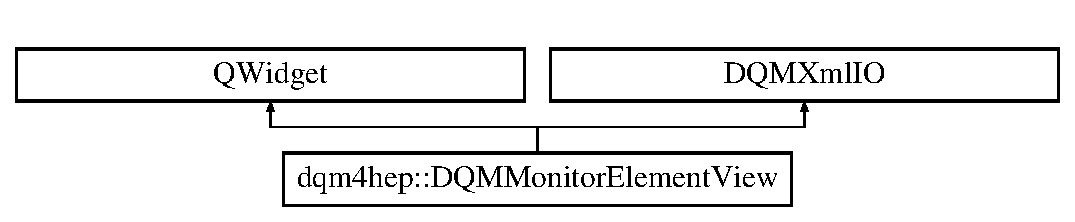
\includegraphics[height=2.000000cm]{classdqm4hep_1_1DQMMonitorElementView}
\end{center}
\end{figure}
\subsection*{Public Slots}
\begin{DoxyCompactItemize}
\item 
void {\bf add\+Monitor\+Element} ({\bf D\+Q\+M\+Gui\+Monitor\+Element} $\ast$p\+Monitor\+Element)
\begin{DoxyCompactList}\small\item\em Add a monitor element to the view. \end{DoxyCompactList}\item 
void {\bf remove\+Monitor\+Element} ({\bf D\+Q\+M\+Gui\+Monitor\+Element} $\ast$p\+Gui\+Monitor\+Element)
\begin{DoxyCompactList}\small\item\em Remove a monitor element from the view. \end{DoxyCompactList}\item 
void {\bf update\+Monitor\+Element} ({\bf D\+Q\+M\+Gui\+Monitor\+Element} $\ast$p\+Monitor\+Element)
\begin{DoxyCompactList}\small\item\em Update the monitor element. \end{DoxyCompactList}\item 
void {\bf replace\+Monitor\+Element} ({\bf D\+Q\+M\+Gui\+Monitor\+Element} $\ast$p\+Old\+Monitor\+Element, {\bf D\+Q\+M\+Gui\+Monitor\+Element} $\ast$p\+New\+Monitor\+Element)
\item 
void {\bf clear} ()
\item 
void {\bf clear} (const std\+::string \&collector\+Name)
\end{DoxyCompactItemize}
\subsection*{Public Member Functions}
\begin{DoxyCompactItemize}
\item 
{\bf D\+Q\+M\+Monitor\+Element\+View} ({\bf D\+Q\+M\+Monitoring} $\ast$p\+Monitoring)
\begin{DoxyCompactList}\small\item\em Constructor. \end{DoxyCompactList}\item 
virtual {\bf $\sim$\+D\+Q\+M\+Monitor\+Element\+View} ()
\begin{DoxyCompactList}\small\item\em Destructor. \end{DoxyCompactList}\item 
{\bf D\+Q\+M\+Monitoring} $\ast$ {\bf get\+Monitoring} () const 
\begin{DoxyCompactList}\small\item\em Get the monitoring instance. \end{DoxyCompactList}\item 
Q\+String\+List {\bf get\+Collector\+Names} () const 
\item 
Q\+List$<$ Q\+Tree\+Widget\+Item $\ast$ $>$ {\bf get\+Checked\+Monitor\+Elements} () const 
\item 
Q\+List$<$ Q\+Tree\+Widget\+Item $\ast$ $>$ {\bf get\+Checked\+Monitor\+Elements} (const std\+::string \&collector\+Name) const 
\item 
void {\bf uncheck\+All\+Monitor\+Elements} (const std\+::string \&collector\+Name)
\item 
void {\bf enable\+Subscription} (const std\+::string \&collector\+Name, bool enable=true)
\begin{DoxyCompactList}\small\item\em Enable subscription of monitor elements. \end{DoxyCompactList}\item 
Ti\+Xml\+Element $\ast$ {\bf to\+Xml} () const 
\begin{DoxyCompactList}\small\item\em Export settings to xml element. \end{DoxyCompactList}\item 
void {\bf from\+Xml} (Ti\+Xml\+Element $\ast$const p\+Xml\+Element)
\begin{DoxyCompactList}\small\item\em Import settings from xml element. \end{DoxyCompactList}\end{DoxyCompactItemize}
\subsection*{Private Slots}
\begin{DoxyCompactItemize}
\item 
void {\bf handle\+Monitor\+Element\+Update} ()
\item 
void {\bf handle\+Monitor\+Element\+Deletion} ()
\end{DoxyCompactItemize}
\subsection*{Private Attributes}
\begin{DoxyCompactItemize}
\item 
{\bf D\+Q\+M\+Monitoring} $\ast$ {\bf m\+\_\+p\+Monitoring}
\item 
Q\+Tool\+Box $\ast$ {\bf m\+\_\+p\+Tool\+Box}
\end{DoxyCompactItemize}


\subsection{Detailed Description}
\doxyref{D\+Q\+M\+Monitor\+Element\+View}{p.}{classdqm4hep_1_1DQMMonitorElementView} class. 

Definition at line 263 of file D\+Q\+M\+Monitor\+Element\+View.\+h.



\subsection{Constructor \& Destructor Documentation}
\index{dqm4hep\+::\+D\+Q\+M\+Monitor\+Element\+View@{dqm4hep\+::\+D\+Q\+M\+Monitor\+Element\+View}!D\+Q\+M\+Monitor\+Element\+View@{D\+Q\+M\+Monitor\+Element\+View}}
\index{D\+Q\+M\+Monitor\+Element\+View@{D\+Q\+M\+Monitor\+Element\+View}!dqm4hep\+::\+D\+Q\+M\+Monitor\+Element\+View@{dqm4hep\+::\+D\+Q\+M\+Monitor\+Element\+View}}
\subsubsection[{D\+Q\+M\+Monitor\+Element\+View}]{\setlength{\rightskip}{0pt plus 5cm}dqm4hep\+::\+D\+Q\+M\+Monitor\+Element\+View\+::\+D\+Q\+M\+Monitor\+Element\+View (
\begin{DoxyParamCaption}
\item[{{\bf D\+Q\+M\+Monitoring} $\ast$}]{p\+Monitoring}
\end{DoxyParamCaption}
)}\label{classdqm4hep_1_1DQMMonitorElementView_a353546c370fc02dd379a2e70fbdc8ef9}


Constructor. 



Definition at line 1196 of file D\+Q\+M\+Monitor\+Element\+View.\+cc.



References m\+\_\+p\+Tool\+Box.


\begin{DoxyCode}
1196                                                                        :
1197     m_pMonitoring(pMonitoring)
1198 \{
1199   setLayout(\textcolor{keyword}{new} QVBoxLayout());
1200 
1201   m_pToolBox = \textcolor{keyword}{new} QToolBox();
1202   layout()->addWidget(m_pToolBox);
1203 \}
\end{DoxyCode}
\index{dqm4hep\+::\+D\+Q\+M\+Monitor\+Element\+View@{dqm4hep\+::\+D\+Q\+M\+Monitor\+Element\+View}!````~D\+Q\+M\+Monitor\+Element\+View@{$\sim$\+D\+Q\+M\+Monitor\+Element\+View}}
\index{````~D\+Q\+M\+Monitor\+Element\+View@{$\sim$\+D\+Q\+M\+Monitor\+Element\+View}!dqm4hep\+::\+D\+Q\+M\+Monitor\+Element\+View@{dqm4hep\+::\+D\+Q\+M\+Monitor\+Element\+View}}
\subsubsection[{$\sim$\+D\+Q\+M\+Monitor\+Element\+View}]{\setlength{\rightskip}{0pt plus 5cm}dqm4hep\+::\+D\+Q\+M\+Monitor\+Element\+View\+::$\sim$\+D\+Q\+M\+Monitor\+Element\+View (
\begin{DoxyParamCaption}
{}
\end{DoxyParamCaption}
)\hspace{0.3cm}{\ttfamily [virtual]}}\label{classdqm4hep_1_1DQMMonitorElementView_a25fb703dd14dc2d656ef70ad19a9f2bf}


Destructor. 



Definition at line 1207 of file D\+Q\+M\+Monitor\+Element\+View.\+cc.


\begin{DoxyCode}
1208 \{
1209   \textcolor{comment}{/* nop */}
1210 \}
\end{DoxyCode}


\subsection{Member Function Documentation}
\index{dqm4hep\+::\+D\+Q\+M\+Monitor\+Element\+View@{dqm4hep\+::\+D\+Q\+M\+Monitor\+Element\+View}!add\+Monitor\+Element@{add\+Monitor\+Element}}
\index{add\+Monitor\+Element@{add\+Monitor\+Element}!dqm4hep\+::\+D\+Q\+M\+Monitor\+Element\+View@{dqm4hep\+::\+D\+Q\+M\+Monitor\+Element\+View}}
\subsubsection[{add\+Monitor\+Element}]{\setlength{\rightskip}{0pt plus 5cm}void dqm4hep\+::\+D\+Q\+M\+Monitor\+Element\+View\+::add\+Monitor\+Element (
\begin{DoxyParamCaption}
\item[{{\bf D\+Q\+M\+Gui\+Monitor\+Element} $\ast$}]{p\+Monitor\+Element}
\end{DoxyParamCaption}
)\hspace{0.3cm}{\ttfamily [slot]}}\label{classdqm4hep_1_1DQMMonitorElementView_a5193e90981fc4e6cc0bb455266598531}


Add a monitor element to the view. 



Definition at line 1410 of file D\+Q\+M\+Monitor\+Element\+View.\+cc.



References update\+Monitor\+Element().



Referenced by dqm4hep\+::\+D\+Q\+M\+Monitoring\+Model\+::get\+Or\+Create\+Gui\+Monitor\+Element(), dqm4hep\+::\+D\+Q\+M\+Monitoring\+Model\+::load\+Monitor\+Element\+Info\+List(), and dqm4hep\+::\+D\+Q\+M\+Monitoring\+Model\+::update\+Monitor\+Element().


\begin{DoxyCode}
1411 \{
1412   this->updateMonitorElement(pMonitorElement);
1413 \}
\end{DoxyCode}
\index{dqm4hep\+::\+D\+Q\+M\+Monitor\+Element\+View@{dqm4hep\+::\+D\+Q\+M\+Monitor\+Element\+View}!clear@{clear}}
\index{clear@{clear}!dqm4hep\+::\+D\+Q\+M\+Monitor\+Element\+View@{dqm4hep\+::\+D\+Q\+M\+Monitor\+Element\+View}}
\subsubsection[{clear}]{\setlength{\rightskip}{0pt plus 5cm}void dqm4hep\+::\+D\+Q\+M\+Monitor\+Element\+View\+::clear (
\begin{DoxyParamCaption}
{}
\end{DoxyParamCaption}
)\hspace{0.3cm}{\ttfamily [slot]}}\label{classdqm4hep_1_1DQMMonitorElementView_abcbf0b748f9ee0f4b34bf88362a3f199}


Definition at line 1473 of file D\+Q\+M\+Monitor\+Element\+View.\+cc.



References dqm4hep\+::\+D\+Q\+M\+Monitor\+Element\+Navigator\+::clear(), and m\+\_\+p\+Tool\+Box.



Referenced by dqm4hep\+::\+D\+Q\+M\+Monitoring\+View\+::clear(), and from\+Xml().


\begin{DoxyCode}
1474 \{
1475   \textcolor{keywordflow}{for}(\textcolor{keywordtype}{int} i=0 ; i<m_pToolBox->count() ; i++)
1476   \{
1477     DQMMonitorElementNavigator *pNavigator = qobject\_cast<DQMMonitorElementNavigator*>(
      m_pToolBox->widget(i));
1478     pNavigator->clear();
1479     m_pToolBox->removeItem(i);
1480     pNavigator->deleteLater();
1481   \}
1482 \}
\end{DoxyCode}
\index{dqm4hep\+::\+D\+Q\+M\+Monitor\+Element\+View@{dqm4hep\+::\+D\+Q\+M\+Monitor\+Element\+View}!clear@{clear}}
\index{clear@{clear}!dqm4hep\+::\+D\+Q\+M\+Monitor\+Element\+View@{dqm4hep\+::\+D\+Q\+M\+Monitor\+Element\+View}}
\subsubsection[{clear}]{\setlength{\rightskip}{0pt plus 5cm}void dqm4hep\+::\+D\+Q\+M\+Monitor\+Element\+View\+::clear (
\begin{DoxyParamCaption}
\item[{const std\+::string \&}]{collector\+Name}
\end{DoxyParamCaption}
)\hspace{0.3cm}{\ttfamily [slot]}}\label{classdqm4hep_1_1DQMMonitorElementView_a99a230dc2a3611e6f507b186c976ce8d}


Definition at line 1486 of file D\+Q\+M\+Monitor\+Element\+View.\+cc.



References dqm4hep\+::\+D\+Q\+M\+Monitor\+Element\+Navigator\+::clear(), and m\+\_\+p\+Tool\+Box.


\begin{DoxyCode}
1487 \{
1488   \textcolor{keywordflow}{for}(\textcolor{keywordtype}{int} i=0 ; i<m_pToolBox->count() ; i++)
1489   \{
1490     \textcolor{keywordflow}{if}(m_pToolBox->itemText(i) == QString(collectorName.c\_str()))
1491     \{
1492       DQMMonitorElementNavigator *pNavigator = qobject\_cast<DQMMonitorElementNavigator*>(
      m_pToolBox->widget(i));
1493       pNavigator->clear();
1494       \textcolor{keywordflow}{break};
1495     \}
1496   \}
1497 \}
\end{DoxyCode}
\index{dqm4hep\+::\+D\+Q\+M\+Monitor\+Element\+View@{dqm4hep\+::\+D\+Q\+M\+Monitor\+Element\+View}!enable\+Subscription@{enable\+Subscription}}
\index{enable\+Subscription@{enable\+Subscription}!dqm4hep\+::\+D\+Q\+M\+Monitor\+Element\+View@{dqm4hep\+::\+D\+Q\+M\+Monitor\+Element\+View}}
\subsubsection[{enable\+Subscription}]{\setlength{\rightskip}{0pt plus 5cm}void dqm4hep\+::\+D\+Q\+M\+Monitor\+Element\+View\+::enable\+Subscription (
\begin{DoxyParamCaption}
\item[{const std\+::string \&}]{collector\+Name, }
\item[{bool}]{enable = {\ttfamily true}}
\end{DoxyParamCaption}
)}\label{classdqm4hep_1_1DQMMonitorElementView_a8ebc160c41eedc78035099468f2f3317}


Enable subscription of monitor elements. 



Definition at line 1285 of file D\+Q\+M\+Monitor\+Element\+View.\+cc.



References dqm4hep\+::\+D\+Q\+M\+Monitor\+Element\+Navigator\+::enable\+Subscription(), and m\+\_\+p\+Tool\+Box.



Referenced by dqm4hep\+::\+D\+Q\+M\+Monitoring\+Controller\+::handle\+Server\+Shutdown(), and dqm4hep\+::\+D\+Q\+M\+Monitoring\+Controller\+::handle\+Server\+Startup().


\begin{DoxyCode}
1286 \{
1287   \textcolor{keywordflow}{for}(\textcolor{keywordtype}{int} i=0 ; i<m_pToolBox->count() ; i++)
1288   \{
1289     \textcolor{keywordflow}{if}(m_pToolBox->itemText(i).toStdString() == collectorName)
1290     \{
1291       DQMMonitorElementNavigator *pNavigator = qobject\_cast<DQMMonitorElementNavigator*>(
      m_pToolBox->widget(i));
1292       pNavigator->enableSubscription(enable);
1293       \textcolor{keywordflow}{break};
1294     \}
1295   \}
1296 \}
\end{DoxyCode}
\index{dqm4hep\+::\+D\+Q\+M\+Monitor\+Element\+View@{dqm4hep\+::\+D\+Q\+M\+Monitor\+Element\+View}!from\+Xml@{from\+Xml}}
\index{from\+Xml@{from\+Xml}!dqm4hep\+::\+D\+Q\+M\+Monitor\+Element\+View@{dqm4hep\+::\+D\+Q\+M\+Monitor\+Element\+View}}
\subsubsection[{from\+Xml}]{\setlength{\rightskip}{0pt plus 5cm}void dqm4hep\+::\+D\+Q\+M\+Monitor\+Element\+View\+::from\+Xml (
\begin{DoxyParamCaption}
\item[{Ti\+Xml\+Element $\ast$const}]{p\+Xml\+Element}
\end{DoxyParamCaption}
)}\label{classdqm4hep_1_1DQMMonitorElementView_ab8b40f991f9e84d693024f8eba292d65}


Import settings from xml element. 



Definition at line 1351 of file D\+Q\+M\+Monitor\+Element\+View.\+cc.



References dqm4hep\+::\+D\+Q\+M\+Monitor\+Element\+Navigator\+::add\+Monitor\+Element(), clear(), get\+Monitoring(), m\+\_\+p\+Tool\+Box, and dqm4hep\+::\+D\+Q\+M\+Monitor\+Element\+Navigator\+::mkdir().



Referenced by dqm4hep\+::\+D\+Q\+M\+Monitoring\+View\+::from\+Xml().


\begin{DoxyCode}
1352 \{
1353   \textcolor{keywordflow}{if}(!pXmlElement)
1354     \textcolor{keywordflow}{return};
1355 
1356   this->clear();
1357 
1358     TiXmlHandle elementHandle(pXmlElement);
1359 
1360     \textcolor{keywordflow}{for} (TiXmlElement *pCollectorElement = elementHandle.FirstChild(\textcolor{stringliteral}{"collector"}).Element(); NULL != 
      pCollectorElement;
1361         pCollectorElement = pCollectorElement->NextSiblingElement(\textcolor{stringliteral}{"collector"}))
1362     \{
1363       std::string collectorName;
1364         \textcolor{keywordflow}{if}(pCollectorElement->QueryStringAttribute(\textcolor{stringliteral}{"name"}, &collectorName))
1365             \textcolor{keywordflow}{continue};
1366 
1367         DQMMonitorElementNavigator *pNavigator = \textcolor{keyword}{new} DQMMonitorElementNavigator(collectorName.c\_str(), 
      this->getMonitoring());
1368     m_pToolBox->addItem(pNavigator, collectorName.c\_str());
1369 
1370         TiXmlHandle collectorHandle(pCollectorElement);
1371 
1372         \textcolor{keywordflow}{for} (TiXmlElement *pModuleElement = collectorHandle.FirstChild(\textcolor{stringliteral}{"module"}).Element(); NULL != 
      pModuleElement;
1373             pModuleElement = pModuleElement->NextSiblingElement(\textcolor{stringliteral}{"module"}))
1374         \{
1375           std::string moduleName;
1376             \textcolor{keywordflow}{if}(pModuleElement->QueryStringAttribute(\textcolor{stringliteral}{"name"}, &moduleName))
1377                 \textcolor{keywordflow}{continue};
1378 
1379             QTreeWidgetItem *pModuleItem = pNavigator->mkdir(moduleName.c\_str());
1380 
1381             TiXmlHandle moduleHandle(pModuleElement);
1382 
1383             \textcolor{keywordflow}{for} (TiXmlElement *pItemElement = moduleHandle.FirstChild(\textcolor{stringliteral}{"item"}).Element(); NULL != 
      pItemElement;
1384                 pItemElement = pItemElement->NextSiblingElement(\textcolor{stringliteral}{"item"}))
1385             \{
1386               std::string name;
1387                 \textcolor{keywordflow}{if}(pItemElement->QueryStringAttribute(\textcolor{stringliteral}{"name"}, &name))
1388                     \textcolor{keywordflow}{continue};
1389 
1390               std::string path;
1391                 \textcolor{keywordflow}{if}(pItemElement->QueryStringAttribute(\textcolor{stringliteral}{"path"}, &path))
1392                     \textcolor{keywordflow}{continue};
1393 
1394               \textcolor{keywordtype}{bool} checked = \textcolor{keyword}{false};
1395                 \textcolor{keywordflow}{if}(pItemElement->QueryValueAttribute(\textcolor{stringliteral}{"checked"}, &checked))
1396                     \textcolor{keywordflow}{continue};
1397 
1398                 QTreeWidgetItem *pDirectoryItem = pNavigator->mkdir(moduleName.c\_str(), path.c\_str());
1399                 QTreeWidgetItem *pMonitorElementItem = pNavigator->addMonitorElement(pDirectoryItem, name.
      c\_str());
1400 
1401                 \textcolor{keywordflow}{if}(pMonitorElementItem)
1402                   pMonitorElementItem->setCheckState(0, checked ? Qt::Checked : Qt::Unchecked);
1403             \}
1404         \}
1405     \}
1406 \}
\end{DoxyCode}
\index{dqm4hep\+::\+D\+Q\+M\+Monitor\+Element\+View@{dqm4hep\+::\+D\+Q\+M\+Monitor\+Element\+View}!get\+Checked\+Monitor\+Elements@{get\+Checked\+Monitor\+Elements}}
\index{get\+Checked\+Monitor\+Elements@{get\+Checked\+Monitor\+Elements}!dqm4hep\+::\+D\+Q\+M\+Monitor\+Element\+View@{dqm4hep\+::\+D\+Q\+M\+Monitor\+Element\+View}}
\subsubsection[{get\+Checked\+Monitor\+Elements}]{\setlength{\rightskip}{0pt plus 5cm}Q\+List$<$ Q\+Tree\+Widget\+Item $\ast$ $>$ dqm4hep\+::\+D\+Q\+M\+Monitor\+Element\+View\+::get\+Checked\+Monitor\+Elements (
\begin{DoxyParamCaption}
{}
\end{DoxyParamCaption}
) const}\label{classdqm4hep_1_1DQMMonitorElementView_a8ec0831c375f368e72c688d426ef4eba}


Definition at line 1233 of file D\+Q\+M\+Monitor\+Element\+View.\+cc.



References dqm4hep\+::\+D\+Q\+M\+Monitor\+Element\+Navigator\+::get\+Checked\+Monitor\+Elements(), and m\+\_\+p\+Tool\+Box.



Referenced by dqm4hep\+::\+D\+Q\+M\+Monitoring\+Controller\+::handle\+Server\+Startup().


\begin{DoxyCode}
1234 \{
1235   QList<QTreeWidgetItem*> checkedMonitorElements;
1236 
1237   \textcolor{keywordflow}{for}(\textcolor{keywordtype}{int} i=0 ; i<m_pToolBox->count() ; i++)
1238   \{
1239     DQMMonitorElementNavigator *pNavigator = qobject\_cast<DQMMonitorElementNavigator*>(
      m_pToolBox->widget(i));
1240     checkedMonitorElements.append(pNavigator->getCheckedMonitorElements());
1241   \}
1242 
1243   \textcolor{keywordflow}{return} checkedMonitorElements;
1244 \}
\end{DoxyCode}
\index{dqm4hep\+::\+D\+Q\+M\+Monitor\+Element\+View@{dqm4hep\+::\+D\+Q\+M\+Monitor\+Element\+View}!get\+Checked\+Monitor\+Elements@{get\+Checked\+Monitor\+Elements}}
\index{get\+Checked\+Monitor\+Elements@{get\+Checked\+Monitor\+Elements}!dqm4hep\+::\+D\+Q\+M\+Monitor\+Element\+View@{dqm4hep\+::\+D\+Q\+M\+Monitor\+Element\+View}}
\subsubsection[{get\+Checked\+Monitor\+Elements}]{\setlength{\rightskip}{0pt plus 5cm}Q\+List$<$ Q\+Tree\+Widget\+Item $\ast$ $>$ dqm4hep\+::\+D\+Q\+M\+Monitor\+Element\+View\+::get\+Checked\+Monitor\+Elements (
\begin{DoxyParamCaption}
\item[{const std\+::string \&}]{collector\+Name}
\end{DoxyParamCaption}
) const}\label{classdqm4hep_1_1DQMMonitorElementView_a49f26a31c9fa765867aa30cb56d71431}


Definition at line 1248 of file D\+Q\+M\+Monitor\+Element\+View.\+cc.



References dqm4hep\+::\+D\+Q\+M\+Monitor\+Element\+Navigator\+::get\+Checked\+Monitor\+Elements(), and m\+\_\+p\+Tool\+Box.


\begin{DoxyCode}
1249 \{
1250   QList<QTreeWidgetItem*> checkedMonitorElements;
1251   DQMMonitorElementNavigator *pNavigator = NULL;
1252 
1253   \textcolor{keywordflow}{for}(\textcolor{keywordtype}{int} i=0 ; i<m_pToolBox->count() ; i++)
1254   \{
1255     \textcolor{keywordflow}{if}(m_pToolBox->itemText(i).toStdString() == collectorName)
1256     \{
1257       pNavigator = qobject\_cast<DQMMonitorElementNavigator*>(m_pToolBox->widget(i));
1258       \textcolor{keywordflow}{break};
1259     \}
1260   \}
1261 
1262   \textcolor{keywordflow}{if}(NULL == pNavigator)
1263     \textcolor{keywordflow}{return} checkedMonitorElements;
1264 
1265   \textcolor{keywordflow}{return} pNavigator->getCheckedMonitorElements();
1266 \}
\end{DoxyCode}
\index{dqm4hep\+::\+D\+Q\+M\+Monitor\+Element\+View@{dqm4hep\+::\+D\+Q\+M\+Monitor\+Element\+View}!get\+Collector\+Names@{get\+Collector\+Names}}
\index{get\+Collector\+Names@{get\+Collector\+Names}!dqm4hep\+::\+D\+Q\+M\+Monitor\+Element\+View@{dqm4hep\+::\+D\+Q\+M\+Monitor\+Element\+View}}
\subsubsection[{get\+Collector\+Names}]{\setlength{\rightskip}{0pt plus 5cm}Q\+String\+List dqm4hep\+::\+D\+Q\+M\+Monitor\+Element\+View\+::get\+Collector\+Names (
\begin{DoxyParamCaption}
{}
\end{DoxyParamCaption}
) const}\label{classdqm4hep_1_1DQMMonitorElementView_a99e1c988be8596cdf26a843024996f34}


Definition at line 1221 of file D\+Q\+M\+Monitor\+Element\+View.\+cc.



References m\+\_\+p\+Tool\+Box.


\begin{DoxyCode}
1222 \{
1223   QStringList collectorNames;
1224 
1225   \textcolor{keywordflow}{for}(\textcolor{keywordtype}{int} i=0 ; i<m_pToolBox->count() ; i++)
1226     collectorNames << m_pToolBox->itemText(i);
1227 
1228   \textcolor{keywordflow}{return} collectorNames;
1229 \}
\end{DoxyCode}
\index{dqm4hep\+::\+D\+Q\+M\+Monitor\+Element\+View@{dqm4hep\+::\+D\+Q\+M\+Monitor\+Element\+View}!get\+Monitoring@{get\+Monitoring}}
\index{get\+Monitoring@{get\+Monitoring}!dqm4hep\+::\+D\+Q\+M\+Monitor\+Element\+View@{dqm4hep\+::\+D\+Q\+M\+Monitor\+Element\+View}}
\subsubsection[{get\+Monitoring}]{\setlength{\rightskip}{0pt plus 5cm}{\bf D\+Q\+M\+Monitoring} $\ast$ dqm4hep\+::\+D\+Q\+M\+Monitor\+Element\+View\+::get\+Monitoring (
\begin{DoxyParamCaption}
{}
\end{DoxyParamCaption}
) const}\label{classdqm4hep_1_1DQMMonitorElementView_a2e008a8f002f9028698611fc7726cab7}


Get the monitoring instance. 



Definition at line 1214 of file D\+Q\+M\+Monitor\+Element\+View.\+cc.



References m\+\_\+p\+Monitoring.



Referenced by from\+Xml(), and update\+Monitor\+Element().


\begin{DoxyCode}
1215 \{
1216   \textcolor{keywordflow}{return} m_pMonitoring;
1217 \}
\end{DoxyCode}
\index{dqm4hep\+::\+D\+Q\+M\+Monitor\+Element\+View@{dqm4hep\+::\+D\+Q\+M\+Monitor\+Element\+View}!handle\+Monitor\+Element\+Deletion@{handle\+Monitor\+Element\+Deletion}}
\index{handle\+Monitor\+Element\+Deletion@{handle\+Monitor\+Element\+Deletion}!dqm4hep\+::\+D\+Q\+M\+Monitor\+Element\+View@{dqm4hep\+::\+D\+Q\+M\+Monitor\+Element\+View}}
\subsubsection[{handle\+Monitor\+Element\+Deletion}]{\setlength{\rightskip}{0pt plus 5cm}void dqm4hep\+::\+D\+Q\+M\+Monitor\+Element\+View\+::handle\+Monitor\+Element\+Deletion (
\begin{DoxyParamCaption}
{}
\end{DoxyParamCaption}
)\hspace{0.3cm}{\ttfamily [private]}, {\ttfamily [slot]}}\label{classdqm4hep_1_1DQMMonitorElementView_a402dd32dd2264a198ddd5985201bd4ea}


Definition at line 1509 of file D\+Q\+M\+Monitor\+Element\+View.\+cc.



References remove\+Monitor\+Element().


\begin{DoxyCode}
1510 \{
1511   DQMGuiMonitorElement *pGuiMonitorElement = qobject\_cast<DQMGuiMonitorElement*>(sender());
1512   this->removeMonitorElement(pGuiMonitorElement);
1513 
1514 \}
\end{DoxyCode}
\index{dqm4hep\+::\+D\+Q\+M\+Monitor\+Element\+View@{dqm4hep\+::\+D\+Q\+M\+Monitor\+Element\+View}!handle\+Monitor\+Element\+Update@{handle\+Monitor\+Element\+Update}}
\index{handle\+Monitor\+Element\+Update@{handle\+Monitor\+Element\+Update}!dqm4hep\+::\+D\+Q\+M\+Monitor\+Element\+View@{dqm4hep\+::\+D\+Q\+M\+Monitor\+Element\+View}}
\subsubsection[{handle\+Monitor\+Element\+Update}]{\setlength{\rightskip}{0pt plus 5cm}void dqm4hep\+::\+D\+Q\+M\+Monitor\+Element\+View\+::handle\+Monitor\+Element\+Update (
\begin{DoxyParamCaption}
{}
\end{DoxyParamCaption}
)\hspace{0.3cm}{\ttfamily [private]}, {\ttfamily [slot]}}\label{classdqm4hep_1_1DQMMonitorElementView_acb6184ed228be4b79e01f04862db1f19}


Definition at line 1501 of file D\+Q\+M\+Monitor\+Element\+View.\+cc.



References update\+Monitor\+Element().


\begin{DoxyCode}
1502 \{
1503   DQMGuiMonitorElement *pGuiMonitorElement = qobject\_cast<DQMGuiMonitorElement*>(sender());
1504   this->updateMonitorElement(pGuiMonitorElement);
1505 \}
\end{DoxyCode}
\index{dqm4hep\+::\+D\+Q\+M\+Monitor\+Element\+View@{dqm4hep\+::\+D\+Q\+M\+Monitor\+Element\+View}!remove\+Monitor\+Element@{remove\+Monitor\+Element}}
\index{remove\+Monitor\+Element@{remove\+Monitor\+Element}!dqm4hep\+::\+D\+Q\+M\+Monitor\+Element\+View@{dqm4hep\+::\+D\+Q\+M\+Monitor\+Element\+View}}
\subsubsection[{remove\+Monitor\+Element}]{\setlength{\rightskip}{0pt plus 5cm}void dqm4hep\+::\+D\+Q\+M\+Monitor\+Element\+View\+::remove\+Monitor\+Element (
\begin{DoxyParamCaption}
\item[{{\bf D\+Q\+M\+Gui\+Monitor\+Element} $\ast$}]{p\+Gui\+Monitor\+Element}
\end{DoxyParamCaption}
)\hspace{0.3cm}{\ttfamily [slot]}}\label{classdqm4hep_1_1DQMMonitorElementView_ad4047f57b6d74bd9920310684edf4d10}


Remove a monitor element from the view. 



Definition at line 1417 of file D\+Q\+M\+Monitor\+Element\+View.\+cc.



References dqm4hep\+::\+D\+Q\+M\+Gui\+Monitor\+Element\+::get\+Monitor\+Element(), m\+\_\+p\+Tool\+Box, and dqm4hep\+::\+D\+Q\+M\+Monitor\+Element\+Navigator\+::remove\+Monitor\+Element().



Referenced by dqm4hep\+::\+D\+Q\+M\+Monitoring\+Model\+::clear(), handle\+Monitor\+Element\+Deletion(), and dqm4hep\+::\+D\+Q\+M\+Monitoring\+Model\+::remove\+Monitor\+Element().


\begin{DoxyCode}
1418 \{
1419   QString collectorName = pMonitorElement->getMonitorElement()->getCollectorName().c\_str();
1420 
1421   DQMMonitorElementNavigator *pNavigator = NULL;
1422 
1423   \textcolor{keywordflow}{for}(\textcolor{keywordtype}{int} i=0 ; i<m_pToolBox->count() ; i++)
1424   \{
1425     \textcolor{keywordflow}{if}(m_pToolBox->itemText(i) == collectorName)
1426     \{
1427       pNavigator = qobject\_cast<DQMMonitorElementNavigator*>(m_pToolBox->widget(i));
1428       \textcolor{keywordflow}{break};
1429     \}
1430   \}
1431 
1432   \textcolor{keywordflow}{if}(NULL == pNavigator)
1433     \textcolor{keywordflow}{return};
1434 
1435   pNavigator->removeMonitorElement(pMonitorElement);
1436 \}
\end{DoxyCode}
\index{dqm4hep\+::\+D\+Q\+M\+Monitor\+Element\+View@{dqm4hep\+::\+D\+Q\+M\+Monitor\+Element\+View}!replace\+Monitor\+Element@{replace\+Monitor\+Element}}
\index{replace\+Monitor\+Element@{replace\+Monitor\+Element}!dqm4hep\+::\+D\+Q\+M\+Monitor\+Element\+View@{dqm4hep\+::\+D\+Q\+M\+Monitor\+Element\+View}}
\subsubsection[{replace\+Monitor\+Element}]{\setlength{\rightskip}{0pt plus 5cm}void dqm4hep\+::\+D\+Q\+M\+Monitor\+Element\+View\+::replace\+Monitor\+Element (
\begin{DoxyParamCaption}
\item[{{\bf D\+Q\+M\+Gui\+Monitor\+Element} $\ast$}]{p\+Old\+Monitor\+Element, }
\item[{{\bf D\+Q\+M\+Gui\+Monitor\+Element} $\ast$}]{p\+New\+Monitor\+Element}
\end{DoxyParamCaption}
)\hspace{0.3cm}{\ttfamily [slot]}}\label{classdqm4hep_1_1DQMMonitorElementView_adc6a66fb2967fc98e7869715afff4896}


Definition at line 1466 of file D\+Q\+M\+Monitor\+Element\+View.\+cc.



References update\+Monitor\+Element().


\begin{DoxyCode}
1467 \{
1468   this->updateMonitorElement(pNewMonitorElement);
1469 \}
\end{DoxyCode}
\index{dqm4hep\+::\+D\+Q\+M\+Monitor\+Element\+View@{dqm4hep\+::\+D\+Q\+M\+Monitor\+Element\+View}!to\+Xml@{to\+Xml}}
\index{to\+Xml@{to\+Xml}!dqm4hep\+::\+D\+Q\+M\+Monitor\+Element\+View@{dqm4hep\+::\+D\+Q\+M\+Monitor\+Element\+View}}
\subsubsection[{to\+Xml}]{\setlength{\rightskip}{0pt plus 5cm}Ti\+Xml\+Element $\ast$ dqm4hep\+::\+D\+Q\+M\+Monitor\+Element\+View\+::to\+Xml (
\begin{DoxyParamCaption}
{}
\end{DoxyParamCaption}
) const}\label{classdqm4hep_1_1DQMMonitorElementView_a48dff184c5f32ea488b22d19b2bc4f47}


Export settings to xml element. 



Definition at line 1300 of file D\+Q\+M\+Monitor\+Element\+View.\+cc.



References dqm4hep\+::\+D\+Q\+M\+Monitor\+Element\+Navigator\+::get\+All\+Monitor\+Element\+Items(), dqm4hep\+::\+D\+Q\+M\+Monitor\+Element\+Navigator\+::get\+Full\+Path\+Name(), dqm4hep\+::\+D\+Q\+M\+Monitor\+Element\+Navigator\+::get\+Module\+Names(), and m\+\_\+p\+Tool\+Box.



Referenced by dqm4hep\+::\+D\+Q\+M\+Monitoring\+View\+::to\+Xml().


\begin{DoxyCode}
1301 \{
1302   TiXmlElement *pXmlElement = \textcolor{keyword}{new} TiXmlElement(\textcolor{stringliteral}{"meView"});
1303 
1304   \textcolor{comment}{// loop over collectors}
1305   \textcolor{keywordflow}{for}(\textcolor{keywordtype}{int} c=0 ; c<m_pToolBox->count() ; c++)
1306   \{
1307     TiXmlElement *pCollectorElement = \textcolor{keyword}{new} TiXmlElement(\textcolor{stringliteral}{"collector"});
1308     pXmlElement->LinkEndChild(pCollectorElement);
1309 
1310     std::string collectorName = m_pToolBox->itemText(c).toStdString();
1311     pCollectorElement->SetAttribute(\textcolor{stringliteral}{"name"}, collectorName);
1312 
1313     DQMMonitorElementNavigator *pNavigator = qobject\_cast<DQMMonitorElementNavigator*>(
      m_pToolBox->widget(c));
1314 
1315     QStringList moduleNames = pNavigator->getModuleNames();
1316 
1317     \textcolor{keywordflow}{for}(\textcolor{keywordtype}{int} m=0 ; m<moduleNames.count() ; m++)
1318     \{
1319       QString moduleName(moduleNames.at(m));
1320 
1321       TiXmlElement *pModuleElement = \textcolor{keyword}{new} TiXmlElement(\textcolor{stringliteral}{"module"});
1322       pCollectorElement->LinkEndChild(pModuleElement);
1323 
1324       pModuleElement->SetAttribute(\textcolor{stringliteral}{"name"}, moduleName.toStdString());
1325 
1326       QList<QTreeWidgetItem*> monitorElementItems = pNavigator->getAllMonitorElementItems(moduleName);
1327 
1328       \textcolor{keywordflow}{for}(\textcolor{keywordtype}{int} i=0 ; i<monitorElementItems.count() ; i++)
1329       \{
1330         QTreeWidgetItem *pMonitorElementItem = monitorElementItems.at(i);
1331 
1332         QString fullPath(pNavigator->getFullPathName(pMonitorElementItem));
1333         QString name(pMonitorElementItem->text(0));
1334         \textcolor{keywordtype}{bool} checked(pMonitorElementItem->checkState(0) == Qt::Checked);
1335 
1336         TiXmlElement *pItemElement = \textcolor{keyword}{new} TiXmlElement(\textcolor{stringliteral}{"item"});
1337         pModuleElement->LinkEndChild(pItemElement);
1338 
1339         pItemElement->SetAttribute(\textcolor{stringliteral}{"path"}, fullPath.toStdString());
1340         pItemElement->SetAttribute(\textcolor{stringliteral}{"name"}, name.toStdString());
1341         pItemElement->SetAttribute(\textcolor{stringliteral}{"checked"}, checked);
1342       \}
1343     \}
1344   \}
1345 
1346   \textcolor{keywordflow}{return} pXmlElement;
1347 \}
\end{DoxyCode}
\index{dqm4hep\+::\+D\+Q\+M\+Monitor\+Element\+View@{dqm4hep\+::\+D\+Q\+M\+Monitor\+Element\+View}!uncheck\+All\+Monitor\+Elements@{uncheck\+All\+Monitor\+Elements}}
\index{uncheck\+All\+Monitor\+Elements@{uncheck\+All\+Monitor\+Elements}!dqm4hep\+::\+D\+Q\+M\+Monitor\+Element\+View@{dqm4hep\+::\+D\+Q\+M\+Monitor\+Element\+View}}
\subsubsection[{uncheck\+All\+Monitor\+Elements}]{\setlength{\rightskip}{0pt plus 5cm}void dqm4hep\+::\+D\+Q\+M\+Monitor\+Element\+View\+::uncheck\+All\+Monitor\+Elements (
\begin{DoxyParamCaption}
\item[{const std\+::string \&}]{collector\+Name}
\end{DoxyParamCaption}
)}\label{classdqm4hep_1_1DQMMonitorElementView_a9706714bdf021b87b59ce0e2fa429b65}


Definition at line 1270 of file D\+Q\+M\+Monitor\+Element\+View.\+cc.



References m\+\_\+p\+Tool\+Box, and dqm4hep\+::\+D\+Q\+M\+Monitor\+Element\+Navigator\+::uncheck\+All\+Monitor\+Elements().



Referenced by dqm4hep\+::\+D\+Q\+M\+Monitoring\+Controller\+::handle\+Server\+Shutdown().


\begin{DoxyCode}
1271 \{
1272   \textcolor{keywordflow}{for}(\textcolor{keywordtype}{int} i=0 ; i<m_pToolBox->count() ; i++)
1273   \{
1274     \textcolor{keywordflow}{if}(m_pToolBox->itemText(i).toStdString() == collectorName)
1275     \{
1276       DQMMonitorElementNavigator *pNavigator = qobject\_cast<DQMMonitorElementNavigator*>(
      m_pToolBox->widget(i));
1277       pNavigator->uncheckAllMonitorElements();
1278       \textcolor{keywordflow}{break};
1279     \}
1280   \}
1281 \}
\end{DoxyCode}
\index{dqm4hep\+::\+D\+Q\+M\+Monitor\+Element\+View@{dqm4hep\+::\+D\+Q\+M\+Monitor\+Element\+View}!update\+Monitor\+Element@{update\+Monitor\+Element}}
\index{update\+Monitor\+Element@{update\+Monitor\+Element}!dqm4hep\+::\+D\+Q\+M\+Monitor\+Element\+View@{dqm4hep\+::\+D\+Q\+M\+Monitor\+Element\+View}}
\subsubsection[{update\+Monitor\+Element}]{\setlength{\rightskip}{0pt plus 5cm}void dqm4hep\+::\+D\+Q\+M\+Monitor\+Element\+View\+::update\+Monitor\+Element (
\begin{DoxyParamCaption}
\item[{{\bf D\+Q\+M\+Gui\+Monitor\+Element} $\ast$}]{p\+Monitor\+Element}
\end{DoxyParamCaption}
)\hspace{0.3cm}{\ttfamily [slot]}}\label{classdqm4hep_1_1DQMMonitorElementView_a11d0566845f05fcddc69da30a8552028}


Update the monitor element. 



Definition at line 1440 of file D\+Q\+M\+Monitor\+Element\+View.\+cc.



References dqm4hep\+::\+D\+Q\+M\+Gui\+Monitor\+Element\+::get\+Monitor\+Element(), get\+Monitoring(), m\+\_\+p\+Tool\+Box, and dqm4hep\+::\+D\+Q\+M\+Monitor\+Element\+Navigator\+::update\+Monitor\+Element().



Referenced by add\+Monitor\+Element(), handle\+Monitor\+Element\+Update(), replace\+Monitor\+Element(), and dqm4hep\+::\+D\+Q\+M\+Monitoring\+Model\+::update\+Monitor\+Element().


\begin{DoxyCode}
1441 \{
1442   QString collectorName = pMonitorElement->getMonitorElement()->getCollectorName().c\_str();
1443 
1444   DQMMonitorElementNavigator *pNavigator = NULL;
1445 
1446   \textcolor{keywordflow}{for}(\textcolor{keywordtype}{int} i=0 ; i<m_pToolBox->count() ; i++)
1447   \{
1448     \textcolor{keywordflow}{if}(m_pToolBox->itemText(i) == collectorName)
1449     \{
1450       pNavigator = qobject\_cast<DQMMonitorElementNavigator*>(m_pToolBox->widget(i));
1451       \textcolor{keywordflow}{break};
1452     \}
1453   \}
1454 
1455   \textcolor{keywordflow}{if}(NULL == pNavigator)
1456   \{
1457     pNavigator = \textcolor{keyword}{new} DQMMonitorElementNavigator(collectorName, this->
      getMonitoring());
1458     m_pToolBox->addItem(pNavigator, collectorName);
1459   \}
1460 
1461   pNavigator->updateMonitorElement(pMonitorElement);
1462 \}
\end{DoxyCode}


\subsection{Member Data Documentation}
\index{dqm4hep\+::\+D\+Q\+M\+Monitor\+Element\+View@{dqm4hep\+::\+D\+Q\+M\+Monitor\+Element\+View}!m\+\_\+p\+Monitoring@{m\+\_\+p\+Monitoring}}
\index{m\+\_\+p\+Monitoring@{m\+\_\+p\+Monitoring}!dqm4hep\+::\+D\+Q\+M\+Monitor\+Element\+View@{dqm4hep\+::\+D\+Q\+M\+Monitor\+Element\+View}}
\subsubsection[{m\+\_\+p\+Monitoring}]{\setlength{\rightskip}{0pt plus 5cm}{\bf D\+Q\+M\+Monitoring}$\ast$ dqm4hep\+::\+D\+Q\+M\+Monitor\+Element\+View\+::m\+\_\+p\+Monitoring\hspace{0.3cm}{\ttfamily [private]}}\label{classdqm4hep_1_1DQMMonitorElementView_a90070a57854004c3deafd63b970360ff}


Definition at line 344 of file D\+Q\+M\+Monitor\+Element\+View.\+h.



Referenced by get\+Monitoring().

\index{dqm4hep\+::\+D\+Q\+M\+Monitor\+Element\+View@{dqm4hep\+::\+D\+Q\+M\+Monitor\+Element\+View}!m\+\_\+p\+Tool\+Box@{m\+\_\+p\+Tool\+Box}}
\index{m\+\_\+p\+Tool\+Box@{m\+\_\+p\+Tool\+Box}!dqm4hep\+::\+D\+Q\+M\+Monitor\+Element\+View@{dqm4hep\+::\+D\+Q\+M\+Monitor\+Element\+View}}
\subsubsection[{m\+\_\+p\+Tool\+Box}]{\setlength{\rightskip}{0pt plus 5cm}Q\+Tool\+Box$\ast$ dqm4hep\+::\+D\+Q\+M\+Monitor\+Element\+View\+::m\+\_\+p\+Tool\+Box\hspace{0.3cm}{\ttfamily [private]}}\label{classdqm4hep_1_1DQMMonitorElementView_abb683ce91da12202d1818d81a42ee55b}


Definition at line 345 of file D\+Q\+M\+Monitor\+Element\+View.\+h.



Referenced by clear(), D\+Q\+M\+Monitor\+Element\+View(), enable\+Subscription(), from\+Xml(), get\+Checked\+Monitor\+Elements(), get\+Collector\+Names(), remove\+Monitor\+Element(), to\+Xml(), uncheck\+All\+Monitor\+Elements(), and update\+Monitor\+Element().



The documentation for this class was generated from the following files\+:\begin{DoxyCompactItemize}
\item 
{\bf D\+Q\+M\+Monitor\+Element\+View.\+h}\item 
{\bf D\+Q\+M\+Monitor\+Element\+View.\+cc}\end{DoxyCompactItemize}

\section{dqm4hep\+:\+:D\+Q\+M\+Monitoring Class Reference}
\label{classdqm4hep_1_1DQMMonitoring}\index{dqm4hep\+::\+D\+Q\+M\+Monitoring@{dqm4hep\+::\+D\+Q\+M\+Monitoring}}


\doxyref{D\+Q\+M\+Monitoring}{p.}{classdqm4hep_1_1DQMMonitoring} class.  




{\ttfamily \#include $<$D\+Q\+M\+Monitoring.\+h$>$}

\subsection*{Public Member Functions}
\begin{DoxyCompactItemize}
\item 
{\bf D\+Q\+M\+Monitoring} ()
\begin{DoxyCompactList}\small\item\em Constructor. \end{DoxyCompactList}\item 
virtual {\bf $\sim$\+D\+Q\+M\+Monitoring} ()
\begin{DoxyCompactList}\small\item\em Destructor. \end{DoxyCompactList}\item 
void {\bf set\+Controller} ({\bf D\+Q\+M\+Monitoring\+Controller} $\ast$p\+Controller)
\begin{DoxyCompactList}\small\item\em Set the monitoring controller. \end{DoxyCompactList}\item 
{\bf D\+Q\+M\+Monitoring\+Controller} $\ast$ {\bf get\+Controller} () const 
\begin{DoxyCompactList}\small\item\em Get the monitoring controller. \end{DoxyCompactList}\item 
void {\bf set\+Model} ({\bf D\+Q\+M\+Monitoring\+Model} $\ast$p\+Model)
\begin{DoxyCompactList}\small\item\em Set the monitoring model. \end{DoxyCompactList}\item 
{\bf D\+Q\+M\+Monitoring\+Model} $\ast$ {\bf get\+Model} () const 
\begin{DoxyCompactList}\small\item\em Get the monitoring model. \end{DoxyCompactList}\item 
void {\bf set\+View} ({\bf D\+Q\+M\+Monitoring\+View} $\ast$p\+View)
\begin{DoxyCompactList}\small\item\em Set the monitoring view. \end{DoxyCompactList}\item 
{\bf D\+Q\+M\+Monitoring\+View} $\ast$ {\bf get\+View} () const 
\begin{DoxyCompactList}\small\item\em get the monitoring controller \end{DoxyCompactList}\end{DoxyCompactItemize}
\subsection*{Protected Attributes}
\begin{DoxyCompactItemize}
\item 
{\bf D\+Q\+M\+Monitoring\+Controller} $\ast$ {\bf m\+\_\+p\+Controller}
\begin{DoxyCompactList}\small\item\em The monitoring controller. \end{DoxyCompactList}\item 
{\bf D\+Q\+M\+Monitoring\+Model} $\ast$ {\bf m\+\_\+p\+Model}
\begin{DoxyCompactList}\small\item\em The monitoring model. \end{DoxyCompactList}\item 
{\bf D\+Q\+M\+Monitoring\+View} $\ast$ {\bf m\+\_\+p\+View}
\begin{DoxyCompactList}\small\item\em The monitoring view. \end{DoxyCompactList}\end{DoxyCompactItemize}


\subsection{Detailed Description}
\doxyref{D\+Q\+M\+Monitoring}{p.}{classdqm4hep_1_1DQMMonitoring} class. 

Definition at line 44 of file D\+Q\+M\+Monitoring.\+h.



\subsection{Constructor \& Destructor Documentation}
\index{dqm4hep\+::\+D\+Q\+M\+Monitoring@{dqm4hep\+::\+D\+Q\+M\+Monitoring}!D\+Q\+M\+Monitoring@{D\+Q\+M\+Monitoring}}
\index{D\+Q\+M\+Monitoring@{D\+Q\+M\+Monitoring}!dqm4hep\+::\+D\+Q\+M\+Monitoring@{dqm4hep\+::\+D\+Q\+M\+Monitoring}}
\subsubsection[{D\+Q\+M\+Monitoring}]{\setlength{\rightskip}{0pt plus 5cm}dqm4hep\+::\+D\+Q\+M\+Monitoring\+::\+D\+Q\+M\+Monitoring (
\begin{DoxyParamCaption}
{}
\end{DoxyParamCaption}
)}\label{classdqm4hep_1_1DQMMonitoring_a9ed7608a683608f813618405d7b87169}


Constructor. 



Definition at line 37 of file D\+Q\+M\+Monitoring.\+cc.


\begin{DoxyCode}
37                              :
38   m_pController(NULL),
39   m_pModel(NULL),
40   m_pView(NULL)
41 \{
42   \textcolor{comment}{/* nop */}
43 \}
\end{DoxyCode}
\index{dqm4hep\+::\+D\+Q\+M\+Monitoring@{dqm4hep\+::\+D\+Q\+M\+Monitoring}!````~D\+Q\+M\+Monitoring@{$\sim$\+D\+Q\+M\+Monitoring}}
\index{````~D\+Q\+M\+Monitoring@{$\sim$\+D\+Q\+M\+Monitoring}!dqm4hep\+::\+D\+Q\+M\+Monitoring@{dqm4hep\+::\+D\+Q\+M\+Monitoring}}
\subsubsection[{$\sim$\+D\+Q\+M\+Monitoring}]{\setlength{\rightskip}{0pt plus 5cm}dqm4hep\+::\+D\+Q\+M\+Monitoring\+::$\sim$\+D\+Q\+M\+Monitoring (
\begin{DoxyParamCaption}
{}
\end{DoxyParamCaption}
)\hspace{0.3cm}{\ttfamily [virtual]}}\label{classdqm4hep_1_1DQMMonitoring_a6750c56ed984f4511e1f90d61e6c4668}


Destructor. 



Definition at line 47 of file D\+Q\+M\+Monitoring.\+cc.



References m\+\_\+p\+Controller, m\+\_\+p\+Model, and m\+\_\+p\+View.


\begin{DoxyCode}
48 \{
49   \textcolor{keywordflow}{if}(m_pController)
50     \textcolor{keyword}{delete} m_pController;
51 
52   \textcolor{keywordflow}{if}(m_pModel)
53     \textcolor{keyword}{delete} m_pModel;
54 
55   \textcolor{keywordflow}{if}(m_pView)
56     \textcolor{keyword}{delete} m_pView;
57 \}
\end{DoxyCode}


\subsection{Member Function Documentation}
\index{dqm4hep\+::\+D\+Q\+M\+Monitoring@{dqm4hep\+::\+D\+Q\+M\+Monitoring}!get\+Controller@{get\+Controller}}
\index{get\+Controller@{get\+Controller}!dqm4hep\+::\+D\+Q\+M\+Monitoring@{dqm4hep\+::\+D\+Q\+M\+Monitoring}}
\subsubsection[{get\+Controller}]{\setlength{\rightskip}{0pt plus 5cm}{\bf D\+Q\+M\+Monitoring\+Controller} $\ast$ dqm4hep\+::\+D\+Q\+M\+Monitoring\+::get\+Controller (
\begin{DoxyParamCaption}
{}
\end{DoxyParamCaption}
) const}\label{classdqm4hep_1_1DQMMonitoring_a2b32d24096586b9b9ba6bc189a284644}


Get the monitoring controller. 



Definition at line 74 of file D\+Q\+M\+Monitoring.\+cc.



References m\+\_\+p\+Controller.



Referenced by dqm4hep\+::\+D\+Q\+M\+Monitoring\+Main\+Window\+::close\+Event(), dqm4hep\+::\+D\+Q\+M\+Monitor\+Element\+Navigator\+::draw\+Selected\+Monitor\+Elements(), dqm4hep\+::\+D\+Q\+M\+Canvas\+Area\+::drop\+Event(), dqm4hep\+::\+D\+Q\+M\+Monitoring\+View\+::handle\+Auto\+Update\+Button\+Clicked(), dqm4hep\+::\+D\+Q\+M\+Browser\+Widget\+::handle\+Collector\+Selection(), dqm4hep\+::\+D\+Q\+M\+Monitor\+Element\+Navigator\+::handle\+Item\+Double\+Click(), dqm4hep\+::\+D\+Q\+M\+Browser\+Widget\+::handle\+Replace\+Button\+Clicked(), dqm4hep\+::\+D\+Q\+M\+Canvas\+View\+::handle\+Save\+As\+Action\+Triggered(), dqm4hep\+::\+D\+Q\+M\+Browser\+Widget\+::handle\+Update\+Button\+Clicked(), dqm4hep\+::\+D\+Q\+M\+Root\+Widget\+::open\+R\+O\+O\+T\+Panel(), dqm4hep\+::\+D\+Q\+M\+Root\+Widget\+::query\+Update(), dqm4hep\+::\+D\+Q\+M\+Monitor\+Element\+Navigator\+::query\+Update(), dqm4hep\+::\+D\+Q\+M\+Root\+Widget\+::save\+As(), dqm4hep\+::\+Tree\+Widget\+Item\+::set\+Data(), dqm4hep\+::\+D\+Q\+M\+Root\+Widget\+::show\+Monitor\+Element\+Info(), dqm4hep\+::\+D\+Q\+M\+Root\+Widget\+::show\+Q\+Test\+Results(), dqm4hep\+::\+D\+Q\+M\+Monitor\+Element\+Navigator\+::start\+Drag(), dqm4hep\+::\+D\+Q\+M\+Monitor\+Element\+Navigator\+::update\+Monitor\+Element(), and dqm4hep\+::\+D\+Q\+M\+Root\+Widget\+::update\+Monitor\+Element().


\begin{DoxyCode}
75 \{
76   \textcolor{keywordflow}{return} m_pController;
77 \}
\end{DoxyCode}
\index{dqm4hep\+::\+D\+Q\+M\+Monitoring@{dqm4hep\+::\+D\+Q\+M\+Monitoring}!get\+Model@{get\+Model}}
\index{get\+Model@{get\+Model}!dqm4hep\+::\+D\+Q\+M\+Monitoring@{dqm4hep\+::\+D\+Q\+M\+Monitoring}}
\subsubsection[{get\+Model}]{\setlength{\rightskip}{0pt plus 5cm}{\bf D\+Q\+M\+Monitoring\+Model} $\ast$ dqm4hep\+::\+D\+Q\+M\+Monitoring\+::get\+Model (
\begin{DoxyParamCaption}
{}
\end{DoxyParamCaption}
) const}\label{classdqm4hep_1_1DQMMonitoring_a085f84ccfcfac14f0105565c361c0d72}


Get the monitoring model. 



Definition at line 94 of file D\+Q\+M\+Monitoring.\+cc.



References m\+\_\+p\+Model.



Referenced by dqm4hep\+::\+D\+Q\+M\+Monitoring\+Controller\+::clear\+Monitoring(), dqm4hep\+::\+D\+Q\+M\+Monitoring\+Controller\+::clear\+View\+And\+Model(), dqm4hep\+::\+D\+Q\+M\+Monitoring\+Controller\+::create\+Empty\+Monitor\+Elements(), dqm4hep\+::\+D\+Q\+M\+Monitor\+Element\+Navigator\+::draw\+Selected\+Monitor\+Elements(), dqm4hep\+::\+D\+Q\+M\+Canvas\+Area\+::drop\+Event(), dqm4hep\+::\+D\+Q\+M\+Canvas\+View\+::from\+Xml(), dqm4hep\+::\+D\+Q\+M\+Monitor\+Element\+Navigator\+::handle\+Item\+Double\+Click(), dqm4hep\+::\+D\+Q\+M\+Monitor\+Element\+Navigator\+::key\+Press\+Event(), dqm4hep\+::\+D\+Q\+M\+Monitoring\+Controller\+::open\+File(), dqm4hep\+::\+D\+Q\+M\+Monitor\+Element\+Navigator\+::query\+Update(), and dqm4hep\+::\+D\+Q\+M\+Monitoring\+Controller\+::receive\+Monitor\+Element\+Publication().


\begin{DoxyCode}
95 \{
96   \textcolor{keywordflow}{return} m_pModel;
97 \}
\end{DoxyCode}
\index{dqm4hep\+::\+D\+Q\+M\+Monitoring@{dqm4hep\+::\+D\+Q\+M\+Monitoring}!get\+View@{get\+View}}
\index{get\+View@{get\+View}!dqm4hep\+::\+D\+Q\+M\+Monitoring@{dqm4hep\+::\+D\+Q\+M\+Monitoring}}
\subsubsection[{get\+View}]{\setlength{\rightskip}{0pt plus 5cm}{\bf D\+Q\+M\+Monitoring\+View} $\ast$ dqm4hep\+::\+D\+Q\+M\+Monitoring\+::get\+View (
\begin{DoxyParamCaption}
{}
\end{DoxyParamCaption}
) const}\label{classdqm4hep_1_1DQMMonitoring_aba6fc86a9f6b82e30c7d62f3da58b0cc}


get the monitoring controller 



Definition at line 114 of file D\+Q\+M\+Monitoring.\+cc.



References m\+\_\+p\+View.



Referenced by dqm4hep\+::\+D\+Q\+M\+Monitoring\+Model\+::clear(), dqm4hep\+::\+D\+Q\+M\+Monitoring\+Controller\+::clear\+Monitoring(), dqm4hep\+::\+D\+Q\+M\+Monitoring\+Controller\+::clear\+View\+And\+Model(), dqm4hep\+::\+D\+Q\+M\+Root\+Widget\+::create\+Context\+Menu(), dqm4hep\+::\+D\+Q\+M\+Monitor\+Element\+Navigator\+::draw\+Selected\+Monitor\+Elements(), dqm4hep\+::\+D\+Q\+M\+Monitoring\+Model\+::get\+Or\+Create\+Gui\+Monitor\+Element(), dqm4hep\+::\+D\+Q\+M\+Monitor\+Element\+Navigator\+::handle\+Item\+Double\+Click(), dqm4hep\+::\+D\+Q\+M\+Monitoring\+Controller\+::handle\+Server\+Shutdown(), dqm4hep\+::\+D\+Q\+M\+Monitoring\+Controller\+::handle\+Server\+Startup(), dqm4hep\+::\+D\+Q\+M\+Monitor\+Element\+Navigator\+::key\+Press\+Event(), dqm4hep\+::\+D\+Q\+M\+Monitoring\+Model\+::load\+Monitor\+Element\+Info\+List(), dqm4hep\+::\+D\+Q\+M\+Monitoring\+Controller\+::log(), dqm4hep\+::\+D\+Q\+M\+Root\+Widget\+::move\+Canvas(), dqm4hep\+::\+D\+Q\+M\+Monitoring\+Controller\+::open\+File(), dqm4hep\+::\+D\+Q\+M\+Root\+Widget\+::remove\+Canvas(), dqm4hep\+::\+D\+Q\+M\+Monitoring\+Model\+::remove\+Monitor\+Element(), dqm4hep\+::\+D\+Q\+M\+Monitoring\+Controller\+::save\+As(), dqm4hep\+::\+D\+Q\+M\+Monitor\+Element\+Navigator\+::show\+Context\+Menu(), and dqm4hep\+::\+D\+Q\+M\+Monitoring\+Model\+::update\+Monitor\+Element().


\begin{DoxyCode}
115 \{
116   \textcolor{keywordflow}{return} m_pView;
117 \}
\end{DoxyCode}
\index{dqm4hep\+::\+D\+Q\+M\+Monitoring@{dqm4hep\+::\+D\+Q\+M\+Monitoring}!set\+Controller@{set\+Controller}}
\index{set\+Controller@{set\+Controller}!dqm4hep\+::\+D\+Q\+M\+Monitoring@{dqm4hep\+::\+D\+Q\+M\+Monitoring}}
\subsubsection[{set\+Controller}]{\setlength{\rightskip}{0pt plus 5cm}void dqm4hep\+::\+D\+Q\+M\+Monitoring\+::set\+Controller (
\begin{DoxyParamCaption}
\item[{{\bf D\+Q\+M\+Monitoring\+Controller} $\ast$}]{p\+Controller}
\end{DoxyParamCaption}
)}\label{classdqm4hep_1_1DQMMonitoring_a85adffed8d8a4245b806a637c03d642e}


Set the monitoring controller. 



Definition at line 61 of file D\+Q\+M\+Monitoring.\+cc.



References m\+\_\+p\+Controller.



Referenced by dqm4hep\+::\+D\+Q\+M\+Monitoring\+Controller\+::\+D\+Q\+M\+Monitoring\+Controller().


\begin{DoxyCode}
62 \{
63   \textcolor{keywordflow}{if}(m_pController == pController)
64     \textcolor{keywordflow}{return};
65 
66   \textcolor{keywordflow}{if}(NULL != m_pController)
67     \textcolor{keyword}{delete} m_pController;
68 
69   m_pController = pController;
70 \}
\end{DoxyCode}
\index{dqm4hep\+::\+D\+Q\+M\+Monitoring@{dqm4hep\+::\+D\+Q\+M\+Monitoring}!set\+Model@{set\+Model}}
\index{set\+Model@{set\+Model}!dqm4hep\+::\+D\+Q\+M\+Monitoring@{dqm4hep\+::\+D\+Q\+M\+Monitoring}}
\subsubsection[{set\+Model}]{\setlength{\rightskip}{0pt plus 5cm}void dqm4hep\+::\+D\+Q\+M\+Monitoring\+::set\+Model (
\begin{DoxyParamCaption}
\item[{{\bf D\+Q\+M\+Monitoring\+Model} $\ast$}]{p\+Model}
\end{DoxyParamCaption}
)}\label{classdqm4hep_1_1DQMMonitoring_a63dfac5b8f234d3dfd2843111085ea33}


Set the monitoring model. 



Definition at line 81 of file D\+Q\+M\+Monitoring.\+cc.



References m\+\_\+p\+Model.



Referenced by dqm4hep\+::\+D\+Q\+M\+Monitoring\+Model\+::\+D\+Q\+M\+Monitoring\+Model().


\begin{DoxyCode}
82 \{
83   \textcolor{keywordflow}{if}(m_pModel == pModel)
84     \textcolor{keywordflow}{return};
85 
86   \textcolor{keywordflow}{if}(NULL != m_pModel)
87     \textcolor{keyword}{delete} m_pModel;
88 
89   m_pModel = pModel;
90 \}
\end{DoxyCode}
\index{dqm4hep\+::\+D\+Q\+M\+Monitoring@{dqm4hep\+::\+D\+Q\+M\+Monitoring}!set\+View@{set\+View}}
\index{set\+View@{set\+View}!dqm4hep\+::\+D\+Q\+M\+Monitoring@{dqm4hep\+::\+D\+Q\+M\+Monitoring}}
\subsubsection[{set\+View}]{\setlength{\rightskip}{0pt plus 5cm}void dqm4hep\+::\+D\+Q\+M\+Monitoring\+::set\+View (
\begin{DoxyParamCaption}
\item[{{\bf D\+Q\+M\+Monitoring\+View} $\ast$}]{p\+View}
\end{DoxyParamCaption}
)}\label{classdqm4hep_1_1DQMMonitoring_a2794c5fecf03acaf9bda2994bdc21e8d}


Set the monitoring view. 



Definition at line 101 of file D\+Q\+M\+Monitoring.\+cc.



References m\+\_\+p\+View.



Referenced by dqm4hep\+::\+D\+Q\+M\+Monitoring\+View\+::\+D\+Q\+M\+Monitoring\+View().


\begin{DoxyCode}
102 \{
103   \textcolor{keywordflow}{if}(m_pView == pView)
104     \textcolor{keywordflow}{return};
105 
106   \textcolor{keywordflow}{if}(NULL != m_pView)
107     \textcolor{keyword}{delete} m_pView;
108 
109   m_pView = pView;
110 \}
\end{DoxyCode}


\subsection{Member Data Documentation}
\index{dqm4hep\+::\+D\+Q\+M\+Monitoring@{dqm4hep\+::\+D\+Q\+M\+Monitoring}!m\+\_\+p\+Controller@{m\+\_\+p\+Controller}}
\index{m\+\_\+p\+Controller@{m\+\_\+p\+Controller}!dqm4hep\+::\+D\+Q\+M\+Monitoring@{dqm4hep\+::\+D\+Q\+M\+Monitoring}}
\subsubsection[{m\+\_\+p\+Controller}]{\setlength{\rightskip}{0pt plus 5cm}{\bf D\+Q\+M\+Monitoring\+Controller}$\ast$ dqm4hep\+::\+D\+Q\+M\+Monitoring\+::m\+\_\+p\+Controller\hspace{0.3cm}{\ttfamily [protected]}}\label{classdqm4hep_1_1DQMMonitoring_ac29c0bea2a3c354152c5d3563d1a55b4}


The monitoring controller. 



Definition at line 81 of file D\+Q\+M\+Monitoring.\+h.



Referenced by get\+Controller(), set\+Controller(), and $\sim$\+D\+Q\+M\+Monitoring().

\index{dqm4hep\+::\+D\+Q\+M\+Monitoring@{dqm4hep\+::\+D\+Q\+M\+Monitoring}!m\+\_\+p\+Model@{m\+\_\+p\+Model}}
\index{m\+\_\+p\+Model@{m\+\_\+p\+Model}!dqm4hep\+::\+D\+Q\+M\+Monitoring@{dqm4hep\+::\+D\+Q\+M\+Monitoring}}
\subsubsection[{m\+\_\+p\+Model}]{\setlength{\rightskip}{0pt plus 5cm}{\bf D\+Q\+M\+Monitoring\+Model}$\ast$ dqm4hep\+::\+D\+Q\+M\+Monitoring\+::m\+\_\+p\+Model\hspace{0.3cm}{\ttfamily [protected]}}\label{classdqm4hep_1_1DQMMonitoring_ad52837a314be74f2889b83441d112eb8}


The monitoring model. 



Definition at line 82 of file D\+Q\+M\+Monitoring.\+h.



Referenced by get\+Model(), set\+Model(), and $\sim$\+D\+Q\+M\+Monitoring().

\index{dqm4hep\+::\+D\+Q\+M\+Monitoring@{dqm4hep\+::\+D\+Q\+M\+Monitoring}!m\+\_\+p\+View@{m\+\_\+p\+View}}
\index{m\+\_\+p\+View@{m\+\_\+p\+View}!dqm4hep\+::\+D\+Q\+M\+Monitoring@{dqm4hep\+::\+D\+Q\+M\+Monitoring}}
\subsubsection[{m\+\_\+p\+View}]{\setlength{\rightskip}{0pt plus 5cm}{\bf D\+Q\+M\+Monitoring\+View}$\ast$ dqm4hep\+::\+D\+Q\+M\+Monitoring\+::m\+\_\+p\+View\hspace{0.3cm}{\ttfamily [protected]}}\label{classdqm4hep_1_1DQMMonitoring_a9d07cdafbab272239687194113b1bf81}


The monitoring view. 



Definition at line 83 of file D\+Q\+M\+Monitoring.\+h.



Referenced by get\+View(), set\+View(), and $\sim$\+D\+Q\+M\+Monitoring().



The documentation for this class was generated from the following files\+:\begin{DoxyCompactItemize}
\item 
{\bf D\+Q\+M\+Monitoring.\+h}\item 
{\bf D\+Q\+M\+Monitoring.\+cc}\end{DoxyCompactItemize}

\section{dqm4hep\+:\+:D\+Q\+M\+Monitoring\+Controller Class Reference}
\label{classdqm4hep_1_1DQMMonitoringController}\index{dqm4hep\+::\+D\+Q\+M\+Monitoring\+Controller@{dqm4hep\+::\+D\+Q\+M\+Monitoring\+Controller}}


\doxyref{D\+Q\+M\+Monitoring\+Controller}{p.}{classdqm4hep_1_1DQMMonitoringController} class.  




{\ttfamily \#include $<$D\+Q\+M\+Monitoring\+Controller.\+h$>$}

Inheritance diagram for dqm4hep\+:\+:D\+Q\+M\+Monitoring\+Controller\+:\begin{figure}[H]
\begin{center}
\leavevmode
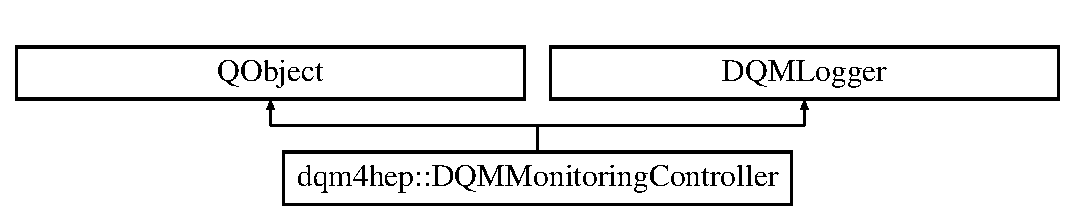
\includegraphics[height=2.000000cm]{classdqm4hep_1_1DQMMonitoringController}
\end{center}
\end{figure}
\subsection*{Public Slots}
\begin{DoxyCompactItemize}
\item 
void {\bf query\+Subscribed\+Monitor\+Elements} ()
\begin{DoxyCompactList}\small\item\em Send a query to the all collectors to send back the subscribed monitor elements. \end{DoxyCompactList}\item 
void {\bf open\+File} ()
\begin{DoxyCompactList}\small\item\em Open a file from a file dialog. \end{DoxyCompactList}\item 
void {\bf open\+File} (const std\+::string \&file\+Name)
\begin{DoxyCompactList}\small\item\em Workhorse of the openfile() method. \end{DoxyCompactList}\item 
void {\bf save\+As} ()
\begin{DoxyCompactList}\small\item\em Open a file dialog and save the current view and model to the target file. \end{DoxyCompactList}\item 
void {\bf save\+As} (const std\+::string \&file\+Name) const 
\begin{DoxyCompactList}\small\item\em Workhorse of the \doxyref{save\+As()}{p.}{classdqm4hep_1_1DQMMonitoringController_a6cb3ef5c0b246a04d57d61283df15d70} method. \end{DoxyCompactList}\item 
void {\bf open\+Browser} ()
\begin{DoxyCompactList}\small\item\em Open a browser widget in a separate window. \end{DoxyCompactList}\item 
void {\bf about\+D\+Q\+M4\+H\+E\+P} ()
\begin{DoxyCompactList}\small\item\em Open about D\+Q\+M4\+H\+E\+P pop up dialog. \end{DoxyCompactList}\item 
void {\bf open\+Doxygen\+Doc} ()
\begin{DoxyCompactList}\small\item\em Open the doxygen documentation (if exists) in the default web browser. \end{DoxyCompactList}\item 
void {\bf open\+User\+Guide} ()
\begin{DoxyCompactList}\small\item\em Open user guide (pdf) in the default pdf reader. \end{DoxyCompactList}\item 
void {\bf open\+Github\+Page} ()
\begin{DoxyCompactList}\small\item\em Open the D\+Q\+M4\+H\+E\+P github page in the default web browser. \end{DoxyCompactList}\item 
void {\bf open\+Issues\+Page} ()
\begin{DoxyCompactList}\small\item\em Open the D\+Q\+M4\+H\+E\+P issues github page in the default web browser. \end{DoxyCompactList}\item 
void {\bf open\+Monitor\+Element\+Info} ({\bf D\+Q\+M\+Gui\+Monitor\+Element} $\ast$p\+Monitor\+Element) const 
\begin{DoxyCompactList}\small\item\em Open a monitor element info widget in a dialog. \end{DoxyCompactList}\item 
void {\bf open\+Quality\+Test\+Results} ({\bf D\+Q\+M\+Gui\+Monitor\+Element} $\ast$p\+Monitor\+Element) const 
\begin{DoxyCompactList}\small\item\em Open a monitor element info widget in a dialog. \end{DoxyCompactList}\item 
void {\bf open\+In\+R\+O\+O\+T\+Window} ({\bf D\+Q\+M\+Gui\+Monitor\+Element} $\ast$p\+Monitor\+Element) const 
\begin{DoxyCompactList}\small\item\em Fork a process and open the monitor element in root canvas. \end{DoxyCompactList}\item 
void {\bf save\+As} ({\bf D\+Q\+M\+Canvas\+Area} $\ast$p\+Canvas\+Area)
\begin{DoxyCompactList}\small\item\em Save all the canvases of the canvas area in a file Different file format available. \end{DoxyCompactList}\item 
void {\bf save\+As} ({\bf D\+Q\+M\+Canvas} $\ast$p\+Canvas)
\begin{DoxyCompactList}\small\item\em Save the canvas in a file Different file format available. \end{DoxyCompactList}\item 
void {\bf clear} ()
\begin{DoxyCompactList}\small\item\em Clear the controller. \end{DoxyCompactList}\item 
void {\bf clear\+View\+And\+Model} ()
\begin{DoxyCompactList}\small\item\em Clear the model and view of the monitoring system. \end{DoxyCompactList}\item 
void {\bf clear\+Monitoring} ()
\begin{DoxyCompactList}\small\item\em Clear the model, view and controller. \end{DoxyCompactList}\item 
void {\bf quit} ()
\begin{DoxyCompactList}\small\item\em Exit the monitoring application. \end{DoxyCompactList}\end{DoxyCompactItemize}
\subsection*{Public Member Functions}
\begin{DoxyCompactItemize}
\item 
{\bf D\+Q\+M\+Monitoring\+Controller} ({\bf D\+Q\+M\+Monitoring} $\ast$p\+Monitoring)
\begin{DoxyCompactList}\small\item\em Constructor. \end{DoxyCompactList}\item 
{\bf $\sim$\+D\+Q\+M\+Monitoring\+Controller} ()
\begin{DoxyCompactList}\small\item\em Destructor. \end{DoxyCompactList}\item 
{\bf D\+Q\+M\+Monitoring} $\ast$ {\bf get\+Monitoring} () const 
\begin{DoxyCompactList}\small\item\em Get the monitoring instance. \end{DoxyCompactList}\item 
void {\bf log} (const std\+::string \&message)
\begin{DoxyCompactList}\small\item\em Log a message in the application. \end{DoxyCompactList}\item 
void {\bf log} (Log\+Level level, const std\+::string \&message)
\begin{DoxyCompactList}\small\item\em Log in the logger with a log level. \end{DoxyCompactList}\item 
{\bf D\+Q\+M\+Gui\+Monitor\+Element\+Client} $\ast$ {\bf create\+Client} (const std\+::string \&collector\+Name)
\begin{DoxyCompactList}\small\item\em Create a monitor element client from the collector name. \end{DoxyCompactList}\item 
{\bf D\+Q\+M\+Gui\+Monitor\+Element\+Client} $\ast$ {\bf get\+Client} (const std\+::string \&collector\+Name)
\begin{DoxyCompactList}\small\item\em Get a registered client. \end{DoxyCompactList}\item 
{\bf D\+Q\+M\+Gui\+Monitor\+Element\+Client} $\ast$ {\bf find\+Client} (const std\+::string \&collector\+Name)
\begin{DoxyCompactList}\small\item\em Find a client. \end{DoxyCompactList}\item 
void {\bf remove\+Client} (const std\+::string \&collector\+Name)
\begin{DoxyCompactList}\small\item\em Remove a client from the application. \end{DoxyCompactList}\item 
void {\bf create\+Empty\+Monitor\+Elements} (const std\+::string \&collector\+Name, const D\+Q\+M\+Monitor\+Element\+Info\+List \&name\+List)
\begin{DoxyCompactList}\small\item\em Fill the model and the view view empty monitor elements. \end{DoxyCompactList}\item 
void {\bf subscribe} (const std\+::string \&collector\+Name, const D\+Q\+M\+Monitor\+Element\+Request \&request)
\begin{DoxyCompactList}\small\item\em Subscribe to monitor elements of the target collector. \end{DoxyCompactList}\item 
void {\bf unsubscribe} (const std\+::string \&collector\+Name, const D\+Q\+M\+Monitor\+Element\+Request \&request)
\begin{DoxyCompactList}\small\item\em Un-\/subscribe to monitor elements of the target collector. \end{DoxyCompactList}\item 
void {\bf query\+Subscribed\+Monitor\+Elements} (const std\+::string \&collector\+Name)
\begin{DoxyCompactList}\small\item\em Send a query to the target collector to send back the subscribed monitor elements. \end{DoxyCompactList}\item 
void {\bf query\+Subscribed\+Monitor\+Elements} (const std\+::string \&collector\+Name, const D\+Q\+M\+Monitor\+Element\+Request \&request)
\begin{DoxyCompactList}\small\item\em Send a query to the target collector to subscribe to the element list (if not done yet) and send back the monitor elements in the request. \end{DoxyCompactList}\item 
void {\bf unsubscribe} (const std\+::string \&collector\+Name)
\begin{DoxyCompactList}\small\item\em Un-\/subscribe to all monitor elements of the target collector. \end{DoxyCompactList}\item 
void {\bf set\+Update\+Mode} (bool update\+Mode)
\begin{DoxyCompactList}\small\item\em Set the update mode of the target collector. \end{DoxyCompactList}\item 
bool {\bf get\+Update\+Mode} () const 
\begin{DoxyCompactList}\small\item\em Get the update mode. \end{DoxyCompactList}\item 
void {\bf query\+Update} ({\bf D\+Q\+M\+Gui\+Monitor\+Element} $\ast$p\+Monitor\+Element)
\begin{DoxyCompactList}\small\item\em Send a query to the collector to first subscribed to the element if not done yet, then to send back the element if collected on the server. \end{DoxyCompactList}\item 
void {\bf query\+Update} (const {\bf D\+Q\+M\+Gui\+Monitor\+Element\+List} \&monitor\+Element\+List)
\begin{DoxyCompactList}\small\item\em Send a query to the collector to first subscribed to the elements if not done yet, then to send back the elements if collected on the server. \end{DoxyCompactList}\item 
Q\+Color {\bf get\+Color} (D\+Q\+M\+Quality quality) const 
\begin{DoxyCompactList}\small\item\em Get the color associated to the data quality. \end{DoxyCompactList}\item 
Q\+Icon {\bf get\+Icon} (D\+Q\+M\+Quality quality) const 
\begin{DoxyCompactList}\small\item\em Get the icon associated to the data quality. \end{DoxyCompactList}\end{DoxyCompactItemize}
\subsection*{Private Types}
\begin{DoxyCompactItemize}
\item 
typedef std\+::map$<$ std\+::string, \\*
{\bf D\+Q\+M\+Gui\+Monitor\+Element\+Client} $\ast$ $>$ {\bf D\+Q\+M\+Gui\+Monitor\+Element\+Client\+Map}
\end{DoxyCompactItemize}
\subsection*{Private Slots}
\begin{DoxyCompactItemize}
\item 
void {\bf receive\+Monitor\+Element\+Publication} (const D\+Q\+M\+Monitor\+Element\+Publication \&publication)
\begin{DoxyCompactList}\small\item\em Call back method called by monitor element clients when a publication is received. \end{DoxyCompactList}\item 
void {\bf handle\+Server\+Startup} ()
\begin{DoxyCompactList}\small\item\em Send the list of subscribed elements to the collector. \end{DoxyCompactList}\item 
void {\bf handle\+Server\+Shutdown} ()
\begin{DoxyCompactList}\small\item\em Send the list of subscribed elements to the collector. \end{DoxyCompactList}\end{DoxyCompactItemize}
\subsection*{Private Attributes}
\begin{DoxyCompactItemize}
\item 
{\bf D\+Q\+M\+Monitoring} $\ast$ {\bf m\+\_\+p\+Monitoring}
\item 
bool {\bf m\+\_\+update\+Mode}
\item 
{\bf D\+Q\+M\+Gui\+Monitor\+Element\+Client\+Map} {\bf m\+\_\+client\+Map}
\item 
Q\+Map$<$ Log\+Level, Q\+String $>$ {\bf m\+\_\+log\+Level\+To\+Text\+Map}
\end{DoxyCompactItemize}


\subsection{Detailed Description}
\doxyref{D\+Q\+M\+Monitoring\+Controller}{p.}{classdqm4hep_1_1DQMMonitoringController} class. 

Definition at line 54 of file D\+Q\+M\+Monitoring\+Controller.\+h.



\subsection{Member Typedef Documentation}
\index{dqm4hep\+::\+D\+Q\+M\+Monitoring\+Controller@{dqm4hep\+::\+D\+Q\+M\+Monitoring\+Controller}!D\+Q\+M\+Gui\+Monitor\+Element\+Client\+Map@{D\+Q\+M\+Gui\+Monitor\+Element\+Client\+Map}}
\index{D\+Q\+M\+Gui\+Monitor\+Element\+Client\+Map@{D\+Q\+M\+Gui\+Monitor\+Element\+Client\+Map}!dqm4hep\+::\+D\+Q\+M\+Monitoring\+Controller@{dqm4hep\+::\+D\+Q\+M\+Monitoring\+Controller}}
\subsubsection[{D\+Q\+M\+Gui\+Monitor\+Element\+Client\+Map}]{\setlength{\rightskip}{0pt plus 5cm}typedef std\+::map$<$std\+::string, {\bf D\+Q\+M\+Gui\+Monitor\+Element\+Client}$\ast$$>$ {\bf dqm4hep\+::\+D\+Q\+M\+Monitoring\+Controller\+::\+D\+Q\+M\+Gui\+Monitor\+Element\+Client\+Map}\hspace{0.3cm}{\ttfamily [private]}}\label{classdqm4hep_1_1DQMMonitoringController_a53d326cd446cbddf37f816136704a1c0}


Definition at line 58 of file D\+Q\+M\+Monitoring\+Controller.\+h.



\subsection{Constructor \& Destructor Documentation}
\index{dqm4hep\+::\+D\+Q\+M\+Monitoring\+Controller@{dqm4hep\+::\+D\+Q\+M\+Monitoring\+Controller}!D\+Q\+M\+Monitoring\+Controller@{D\+Q\+M\+Monitoring\+Controller}}
\index{D\+Q\+M\+Monitoring\+Controller@{D\+Q\+M\+Monitoring\+Controller}!dqm4hep\+::\+D\+Q\+M\+Monitoring\+Controller@{dqm4hep\+::\+D\+Q\+M\+Monitoring\+Controller}}
\subsubsection[{D\+Q\+M\+Monitoring\+Controller}]{\setlength{\rightskip}{0pt plus 5cm}dqm4hep\+::\+D\+Q\+M\+Monitoring\+Controller\+::\+D\+Q\+M\+Monitoring\+Controller (
\begin{DoxyParamCaption}
\item[{{\bf D\+Q\+M\+Monitoring} $\ast$}]{p\+Monitoring}
\end{DoxyParamCaption}
)}\label{classdqm4hep_1_1DQMMonitoringController_a86ccd2de053e059a20c4ac6599356d3d}


Constructor. 



Definition at line 66 of file D\+Q\+M\+Monitoring\+Controller.\+cc.



References m\+\_\+log\+Level\+To\+Text\+Map, m\+\_\+p\+Monitoring, and dqm4hep\+::\+D\+Q\+M\+Monitoring\+::set\+Controller().


\begin{DoxyCode}
66                                                                            :
67   m_pMonitoring(pMonitoring),
68   m_updateMode(\textcolor{keyword}{false})
69 \{
70   m_pMonitoring->setController(\textcolor{keyword}{this});
71 
72   m_logLevelToTextMap.insert(DEBUG, \textcolor{stringliteral}{"[DEBUG] "});
73   m_logLevelToTextMap.insert(MESSAGE, \textcolor{stringliteral}{"[MESSAGE] "});
74   m_logLevelToTextMap.insert(WARNING, \textcolor{stringliteral}{"[WARNING] "});
75   m_logLevelToTextMap.insert(ERROR, \textcolor{stringliteral}{"[ERROR] "});
76 \}
\end{DoxyCode}
\index{dqm4hep\+::\+D\+Q\+M\+Monitoring\+Controller@{dqm4hep\+::\+D\+Q\+M\+Monitoring\+Controller}!````~D\+Q\+M\+Monitoring\+Controller@{$\sim$\+D\+Q\+M\+Monitoring\+Controller}}
\index{````~D\+Q\+M\+Monitoring\+Controller@{$\sim$\+D\+Q\+M\+Monitoring\+Controller}!dqm4hep\+::\+D\+Q\+M\+Monitoring\+Controller@{dqm4hep\+::\+D\+Q\+M\+Monitoring\+Controller}}
\subsubsection[{$\sim$\+D\+Q\+M\+Monitoring\+Controller}]{\setlength{\rightskip}{0pt plus 5cm}dqm4hep\+::\+D\+Q\+M\+Monitoring\+Controller\+::$\sim$\+D\+Q\+M\+Monitoring\+Controller (
\begin{DoxyParamCaption}
{}
\end{DoxyParamCaption}
)}\label{classdqm4hep_1_1DQMMonitoringController_a5d57afd156cb65397d6a5db380c4ffba}


Destructor. 



Definition at line 80 of file D\+Q\+M\+Monitoring\+Controller.\+cc.



References clear().


\begin{DoxyCode}
81 \{
82   clear();
83 \}
\end{DoxyCode}


\subsection{Member Function Documentation}
\index{dqm4hep\+::\+D\+Q\+M\+Monitoring\+Controller@{dqm4hep\+::\+D\+Q\+M\+Monitoring\+Controller}!about\+D\+Q\+M4\+H\+E\+P@{about\+D\+Q\+M4\+H\+E\+P}}
\index{about\+D\+Q\+M4\+H\+E\+P@{about\+D\+Q\+M4\+H\+E\+P}!dqm4hep\+::\+D\+Q\+M\+Monitoring\+Controller@{dqm4hep\+::\+D\+Q\+M\+Monitoring\+Controller}}
\subsubsection[{about\+D\+Q\+M4\+H\+E\+P}]{\setlength{\rightskip}{0pt plus 5cm}void dqm4hep\+::\+D\+Q\+M\+Monitoring\+Controller\+::about\+D\+Q\+M4\+H\+E\+P (
\begin{DoxyParamCaption}
{}
\end{DoxyParamCaption}
)\hspace{0.3cm}{\ttfamily [slot]}}\label{classdqm4hep_1_1DQMMonitoringController_a4d07fc57553a1b4d6bb6567de01af6be}


Open about D\+Q\+M4\+H\+E\+P pop up dialog. 



Definition at line 642 of file D\+Q\+M\+Monitoring\+Controller.\+cc.



References D\+Q\+M\+Viz\+\_\+\+D\+I\+R, D\+Q\+M\+Viz\+\_\+\+V\+E\+R\+S\+I\+O\+N\+\_\+\+S\+T\+R, and get\+Monitoring().


\begin{DoxyCode}
643 \{
644   QString iconDir = QString(DQMViz_DIR) + \textcolor{stringliteral}{"/icons"};
645 
646 
647   QStringList authorList;
648 
649   authorList << \textcolor{stringliteral}{"R. Ete , IPNL"}
650       << \textcolor{stringliteral}{"A. Pingault, GHENT"}
651       << \textcolor{stringliteral}{"L. Mirabito, IPNL"};
652 
653   QString text;
654 
655   text += \textcolor{stringliteral}{"DQMHEP : Data Quality Monitoring for High Energy Physics\(\backslash\)n\(\backslash\)n"};
656   text += \textcolor{stringliteral}{"Version : "}+ QString(DQMViz_VERSION_STR) + \textcolor{stringliteral}{"\(\backslash\)n\(\backslash\)n"};
657 
658   text += \textcolor{stringliteral}{"DQM4HEP is free software: you can redistribute it and/or modify "};
659   text += \textcolor{stringliteral}{"it under the terms of the GNU General Public License as published by"};
660   text += \textcolor{stringliteral}{"the Free Software Foundation, either version 3 of the License, or"};
661   text += \textcolor{stringliteral}{"(at your option) any later version.\(\backslash\)n\(\backslash\)n"};
662 
663   text += \textcolor{stringliteral}{"DQM4HEP is distributed in the hope that it will be useful,"};
664   text += \textcolor{stringliteral}{"but WITHOUT ANY WARRANTY; without even the implied warranty of"};
665   text += \textcolor{stringliteral}{"MERCHANTABILITY or FITNESS FOR A PARTICULAR PURPOSE.  See the"};
666   text += \textcolor{stringliteral}{"GNU General Public License for more details.\(\backslash\)n\(\backslash\)n"};
667 
668   text += \textcolor{stringliteral}{"You should have received a copy of the GNU General Public License"};
669   text += \textcolor{stringliteral}{"along with DQM4HEP. If not, see <http://www.gnu.org/licenses/>.\(\backslash\)n\(\backslash\)n"};
670 
671   text += \textcolor{stringliteral}{"Authors :\(\backslash\)n"};
672   text += \textcolor{stringliteral}{"  * R. Ete , IPNL\(\backslash\)n"};
673   text += \textcolor{stringliteral}{"  * A. Pingault, Ghent University\(\backslash\)n"};
674   text += \textcolor{stringliteral}{"  * L. Mirabito, IPNL\(\backslash\)n\(\backslash\)n"};
675 
676   text += \textcolor{stringliteral}{"Please, send comments or report bug via the github interface "};
677   text += \textcolor{stringliteral}{"<https://github.com/DQM4HEP/DQMViz/issues>"};
678 
679   QMessageBox *pMessageBox = \textcolor{keyword}{new} QMessageBox(this->getMonitoring()->getView()->getMainWindow());
680   pMessageBox->setWindowTitle(\textcolor{stringliteral}{"About DQM4HEP"});
681   pMessageBox->setIconPixmap(QPixmap(iconDir + \textcolor{stringliteral}{"/MON\_WIN.png"}).scaled(QSize(100, 100), 
      Qt::KeepAspectRatioByExpanding));
682   pMessageBox->setText(text);
683 
684   pMessageBox->exec();
685   pMessageBox->deleteLater();
686 \}
\end{DoxyCode}
\index{dqm4hep\+::\+D\+Q\+M\+Monitoring\+Controller@{dqm4hep\+::\+D\+Q\+M\+Monitoring\+Controller}!clear@{clear}}
\index{clear@{clear}!dqm4hep\+::\+D\+Q\+M\+Monitoring\+Controller@{dqm4hep\+::\+D\+Q\+M\+Monitoring\+Controller}}
\subsubsection[{clear}]{\setlength{\rightskip}{0pt plus 5cm}void dqm4hep\+::\+D\+Q\+M\+Monitoring\+Controller\+::clear (
\begin{DoxyParamCaption}
{}
\end{DoxyParamCaption}
)\hspace{0.3cm}{\ttfamily [slot]}}\label{classdqm4hep_1_1DQMMonitoringController_ab5894f200d9ff8d6b2d20edefa1b94e6}


Clear the controller. 

This will remove all client connections. The view and model are not clear. Use \doxyref{clear\+View\+And\+Model()}{p.}{classdqm4hep_1_1DQMMonitoringController_af812e83aeeb73a711d059a8c04826621} to clear only the model and view or use \doxyref{clear\+Monitoring()}{p.}{classdqm4hep_1_1DQMMonitoringController_adcf13668d18a337794d38cb61cfd29d9} to clear the model, view and controller. 

Definition at line 1000 of file D\+Q\+M\+Monitoring\+Controller.\+cc.



References m\+\_\+client\+Map, and m\+\_\+update\+Mode.



Referenced by clear\+Monitoring(), open\+File(), and $\sim$\+D\+Q\+M\+Monitoring\+Controller().


\begin{DoxyCode}
1001 \{
1002   \textcolor{keywordflow}{for}(DQMGuiMonitorElementClientMap::iterator iter = m_clientMap.begin(), endIter = 
      m_clientMap.end() ;
1003       endIter != iter ; ++iter)
1004   \{
1005     iter->second->deleteLater();
1006   \}
1007 
1008   m_clientMap.clear();
1009   m_updateMode = \textcolor{keyword}{false};
1010 \}
\end{DoxyCode}
\index{dqm4hep\+::\+D\+Q\+M\+Monitoring\+Controller@{dqm4hep\+::\+D\+Q\+M\+Monitoring\+Controller}!clear\+Monitoring@{clear\+Monitoring}}
\index{clear\+Monitoring@{clear\+Monitoring}!dqm4hep\+::\+D\+Q\+M\+Monitoring\+Controller@{dqm4hep\+::\+D\+Q\+M\+Monitoring\+Controller}}
\subsubsection[{clear\+Monitoring}]{\setlength{\rightskip}{0pt plus 5cm}void dqm4hep\+::\+D\+Q\+M\+Monitoring\+Controller\+::clear\+Monitoring (
\begin{DoxyParamCaption}
{}
\end{DoxyParamCaption}
)\hspace{0.3cm}{\ttfamily [slot]}}\label{classdqm4hep_1_1DQMMonitoringController_adcf13668d18a337794d38cb61cfd29d9}


Clear the model, view and controller. 



Definition at line 1022 of file D\+Q\+M\+Monitoring\+Controller.\+cc.



References dqm4hep\+::\+D\+Q\+M\+Monitoring\+Model\+::clear(), dqm4hep\+::\+D\+Q\+M\+Monitoring\+View\+::clear(), clear(), dqm4hep\+::\+D\+Q\+M\+Monitoring\+::get\+Model(), get\+Monitoring(), and dqm4hep\+::\+D\+Q\+M\+Monitoring\+::get\+View().



Referenced by quit().


\begin{DoxyCode}
1023 \{
1024   \textcolor{comment}{// first clear the client connections to avoid updates}
1025   this->clear();
1026 
1027   \textcolor{comment}{// clear contents}
1028   this->getMonitoring()->getView()->clear();
1029   this->getMonitoring()->getModel()->clear();
1030 \}
\end{DoxyCode}
\index{dqm4hep\+::\+D\+Q\+M\+Monitoring\+Controller@{dqm4hep\+::\+D\+Q\+M\+Monitoring\+Controller}!clear\+View\+And\+Model@{clear\+View\+And\+Model}}
\index{clear\+View\+And\+Model@{clear\+View\+And\+Model}!dqm4hep\+::\+D\+Q\+M\+Monitoring\+Controller@{dqm4hep\+::\+D\+Q\+M\+Monitoring\+Controller}}
\subsubsection[{clear\+View\+And\+Model}]{\setlength{\rightskip}{0pt plus 5cm}void dqm4hep\+::\+D\+Q\+M\+Monitoring\+Controller\+::clear\+View\+And\+Model (
\begin{DoxyParamCaption}
{}
\end{DoxyParamCaption}
)\hspace{0.3cm}{\ttfamily [slot]}}\label{classdqm4hep_1_1DQMMonitoringController_af812e83aeeb73a711d059a8c04826621}


Clear the model and view of the monitoring system. 

The clients update mode is set to false, disabling automatic updates. The client connections are not removed. Use \doxyref{clear\+Monitoring()}{p.}{classdqm4hep_1_1DQMMonitoringController_adcf13668d18a337794d38cb61cfd29d9} to also clear the client connections. Use \doxyref{clear()}{p.}{classdqm4hep_1_1DQMMonitoringController_ab5894f200d9ff8d6b2d20edefa1b94e6} to clear only the client connections and keep the view and model 

Definition at line 1014 of file D\+Q\+M\+Monitoring\+Controller.\+cc.



References dqm4hep\+::\+D\+Q\+M\+Monitoring\+Model\+::clear(), dqm4hep\+::\+D\+Q\+M\+Monitoring\+View\+::clear(), dqm4hep\+::\+D\+Q\+M\+Monitoring\+::get\+Model(), get\+Monitoring(), and dqm4hep\+::\+D\+Q\+M\+Monitoring\+::get\+View().



Referenced by dqm4hep\+::\+D\+Q\+M\+Browser\+Widget\+::handle\+Replace\+Button\+Clicked().


\begin{DoxyCode}
1015 \{
1016   this->getMonitoring()->getView()->clear();
1017   this->getMonitoring()->getModel()->clear();
1018 \}
\end{DoxyCode}
\index{dqm4hep\+::\+D\+Q\+M\+Monitoring\+Controller@{dqm4hep\+::\+D\+Q\+M\+Monitoring\+Controller}!create\+Client@{create\+Client}}
\index{create\+Client@{create\+Client}!dqm4hep\+::\+D\+Q\+M\+Monitoring\+Controller@{dqm4hep\+::\+D\+Q\+M\+Monitoring\+Controller}}
\subsubsection[{create\+Client}]{\setlength{\rightskip}{0pt plus 5cm}{\bf D\+Q\+M\+Gui\+Monitor\+Element\+Client} $\ast$ dqm4hep\+::\+D\+Q\+M\+Monitoring\+Controller\+::create\+Client (
\begin{DoxyParamCaption}
\item[{const std\+::string \&}]{collector\+Name}
\end{DoxyParamCaption}
)}\label{classdqm4hep_1_1DQMMonitoringController_a288586b8038837bf5c3bc6fddb1206ca}


Create a monitor element client from the collector name. 

Act as a factory method. The client is not registered. To get a registered client, use get\+Client(n) instead 

Definition at line 109 of file D\+Q\+M\+Monitoring\+Controller.\+cc.



Referenced by dqm4hep\+::\+D\+Q\+M\+Browser\+Widget\+::handle\+Collector\+Selection().


\begin{DoxyCode}
110 \{
111   std::cout << \textcolor{stringliteral}{"Creating collector client for "} << collectorName << std::endl;
112   \textcolor{keywordflow}{return} \textcolor{keyword}{new} DQMGuiMonitorElementClient(collectorName);
113 \}
\end{DoxyCode}
\index{dqm4hep\+::\+D\+Q\+M\+Monitoring\+Controller@{dqm4hep\+::\+D\+Q\+M\+Monitoring\+Controller}!create\+Empty\+Monitor\+Elements@{create\+Empty\+Monitor\+Elements}}
\index{create\+Empty\+Monitor\+Elements@{create\+Empty\+Monitor\+Elements}!dqm4hep\+::\+D\+Q\+M\+Monitoring\+Controller@{dqm4hep\+::\+D\+Q\+M\+Monitoring\+Controller}}
\subsubsection[{create\+Empty\+Monitor\+Elements}]{\setlength{\rightskip}{0pt plus 5cm}void dqm4hep\+::\+D\+Q\+M\+Monitoring\+Controller\+::create\+Empty\+Monitor\+Elements (
\begin{DoxyParamCaption}
\item[{const std\+::string \&}]{collector\+Name, }
\item[{const D\+Q\+M\+Monitor\+Element\+Info\+List \&}]{name\+List}
\end{DoxyParamCaption}
)}\label{classdqm4hep_1_1DQMMonitoringController_a8450935f1f1f8d7cf42eb989f202a04c}


Fill the model and the view view empty monitor elements. 

Empty monitor elements are created. If draw action is requested, a 'no viz' canvas will be drawn 

Definition at line 170 of file D\+Q\+M\+Monitoring\+Controller.\+cc.



References dqm4hep\+::\+D\+Q\+M\+Monitoring\+::get\+Model(), get\+Monitoring(), and dqm4hep\+::\+D\+Q\+M\+Monitoring\+Model\+::load\+Monitor\+Element\+Info\+List().



Referenced by dqm4hep\+::\+D\+Q\+M\+Browser\+Widget\+::handle\+Replace\+Button\+Clicked(), and dqm4hep\+::\+D\+Q\+M\+Browser\+Widget\+::handle\+Update\+Button\+Clicked().


\begin{DoxyCode}
171 \{
172   this->getMonitoring()->getModel()->loadMonitorElementInfoList(collectorName, nameList);
173 \}
\end{DoxyCode}
\index{dqm4hep\+::\+D\+Q\+M\+Monitoring\+Controller@{dqm4hep\+::\+D\+Q\+M\+Monitoring\+Controller}!find\+Client@{find\+Client}}
\index{find\+Client@{find\+Client}!dqm4hep\+::\+D\+Q\+M\+Monitoring\+Controller@{dqm4hep\+::\+D\+Q\+M\+Monitoring\+Controller}}
\subsubsection[{find\+Client}]{\setlength{\rightskip}{0pt plus 5cm}{\bf D\+Q\+M\+Gui\+Monitor\+Element\+Client} $\ast$ dqm4hep\+::\+D\+Q\+M\+Monitoring\+Controller\+::find\+Client (
\begin{DoxyParamCaption}
\item[{const std\+::string \&}]{collector\+Name}
\end{DoxyParamCaption}
)}\label{classdqm4hep_1_1DQMMonitoringController_ab17ea76ffed94ac5060a190c60040285}


Find a client. 

Returns N\+U\+L\+L is not registered 

Definition at line 144 of file D\+Q\+M\+Monitoring\+Controller.\+cc.



References m\+\_\+client\+Map.


\begin{DoxyCode}
145 \{
146   DQMGuiMonitorElementClientMap::iterator findIter = m_clientMap.find(collectorName);
147 
148   \textcolor{keywordflow}{if}(m_clientMap.end() != findIter)
149     \textcolor{keywordflow}{return} findIter->second;
150 
151   \textcolor{keywordflow}{return} NULL;
152 \}
\end{DoxyCode}
\index{dqm4hep\+::\+D\+Q\+M\+Monitoring\+Controller@{dqm4hep\+::\+D\+Q\+M\+Monitoring\+Controller}!get\+Client@{get\+Client}}
\index{get\+Client@{get\+Client}!dqm4hep\+::\+D\+Q\+M\+Monitoring\+Controller@{dqm4hep\+::\+D\+Q\+M\+Monitoring\+Controller}}
\subsubsection[{get\+Client}]{\setlength{\rightskip}{0pt plus 5cm}{\bf D\+Q\+M\+Gui\+Monitor\+Element\+Client} $\ast$ dqm4hep\+::\+D\+Q\+M\+Monitoring\+Controller\+::get\+Client (
\begin{DoxyParamCaption}
\item[{const std\+::string \&}]{collector\+Name}
\end{DoxyParamCaption}
)}\label{classdqm4hep_1_1DQMMonitoringController_abf10fb9290358802f6001f93cf8b7fe3}


Get a registered client. 

If the client is not registered, it is created and added on the fly to the list of registered clients 

Definition at line 117 of file D\+Q\+M\+Monitoring\+Controller.\+cc.



References handle\+Server\+Shutdown(), handle\+Server\+Startup(), m\+\_\+client\+Map, m\+\_\+update\+Mode, and receive\+Monitor\+Element\+Publication().



Referenced by dqm4hep\+::\+D\+Q\+M\+Browser\+Widget\+::handle\+Replace\+Button\+Clicked(), dqm4hep\+::\+D\+Q\+M\+Browser\+Widget\+::handle\+Update\+Button\+Clicked(), open\+File(), query\+Subscribed\+Monitor\+Elements(), subscribe(), and unsubscribe().


\begin{DoxyCode}
118 \{
119   DQMGuiMonitorElementClientMap::iterator findIter = m_clientMap.find(collectorName);
120 
121   \textcolor{keywordflow}{if}(m_clientMap.end() != findIter)
122     \textcolor{keywordflow}{return} findIter->second;
123 
124   DQMGuiMonitorElementClient *pNewClient = this->createClient(collectorName);
125 
126   \textcolor{comment}{// to receive monitor elements}
127   connect(pNewClient, SIGNAL(monitorElementPublicationReceived(\textcolor{keyword}{const} DQMMonitorElementPublication &)),
128       \textcolor{keyword}{this}, SLOT(receiveMonitorElementPublication(\textcolor{keyword}{const} DQMMonitorElementPublication &)));
129 
130   \textcolor{comment}{// to handle server startup}
131   connect(pNewClient, SIGNAL(onServerStartup()), \textcolor{keyword}{this}, SLOT(handleServerStartup()));
132 
133   \textcolor{comment}{// to handle server shutdown}
134   connect(pNewClient, SIGNAL(onServerShutdown()), \textcolor{keyword}{this}, SLOT(
      handleServerShutdown()));
135 
136   m_clientMap.insert(DQMGuiMonitorElementClientMap::value\_type(collectorName, pNewClient));
137 
138   pNewClient->getMonitorElementClient()->setUpdateMode(m_updateMode);
139   \textcolor{keywordflow}{return} pNewClient;
140 \}
\end{DoxyCode}
\index{dqm4hep\+::\+D\+Q\+M\+Monitoring\+Controller@{dqm4hep\+::\+D\+Q\+M\+Monitoring\+Controller}!get\+Color@{get\+Color}}
\index{get\+Color@{get\+Color}!dqm4hep\+::\+D\+Q\+M\+Monitoring\+Controller@{dqm4hep\+::\+D\+Q\+M\+Monitoring\+Controller}}
\subsubsection[{get\+Color}]{\setlength{\rightskip}{0pt plus 5cm}Q\+Color dqm4hep\+::\+D\+Q\+M\+Monitoring\+Controller\+::get\+Color (
\begin{DoxyParamCaption}
\item[{D\+Q\+M\+Quality}]{quality}
\end{DoxyParamCaption}
) const}\label{classdqm4hep_1_1DQMMonitoringController_a957df1b44abd383c7910a4066d180f1b}


Get the color associated to the data quality. 



Definition at line 429 of file D\+Q\+M\+Monitoring\+Controller.\+cc.


\begin{DoxyCode}
430 \{
431   QMap<DQMQuality, QColor> colorPalette;
432 
433   colorPalette.insert(NO\_QUALITY, QColor(Qt::gray));
434   colorPalette.insert(VERY\_BAD\_QUALITY, QColor(Qt::darkRed));
435   colorPalette.insert(BAD\_QUALITY, QColor(Qt::darkYellow));
436   colorPalette.insert(NORMAL\_QUALITY, QColor(Qt::black));
437   colorPalette.insert(GOOD\_QUALITY, QColor(Qt::darkBlue));
438   colorPalette.insert(VERY\_GOOD\_QUALITY, QColor(Qt::darkGreen));
439 
440   QMap<DQMQuality, QColor>::const\_iterator findIter = colorPalette.find(quality);
441 
442   \textcolor{keywordflow}{if}(colorPalette.end() == findIter)
443     \textcolor{keywordflow}{return} colorPalette[NO\_QUALITY];
444 
445   \textcolor{keywordflow}{return} findIter.value();
446 \}
\end{DoxyCode}
\index{dqm4hep\+::\+D\+Q\+M\+Monitoring\+Controller@{dqm4hep\+::\+D\+Q\+M\+Monitoring\+Controller}!get\+Icon@{get\+Icon}}
\index{get\+Icon@{get\+Icon}!dqm4hep\+::\+D\+Q\+M\+Monitoring\+Controller@{dqm4hep\+::\+D\+Q\+M\+Monitoring\+Controller}}
\subsubsection[{get\+Icon}]{\setlength{\rightskip}{0pt plus 5cm}Q\+Icon dqm4hep\+::\+D\+Q\+M\+Monitoring\+Controller\+::get\+Icon (
\begin{DoxyParamCaption}
\item[{D\+Q\+M\+Quality}]{quality}
\end{DoxyParamCaption}
) const}\label{classdqm4hep_1_1DQMMonitoringController_a9be19614fbcf6812f41115635bf306f7}


Get the icon associated to the data quality. 



Definition at line 450 of file D\+Q\+M\+Monitoring\+Controller.\+cc.



References D\+Q\+M\+Viz\+\_\+\+D\+I\+R.



Referenced by dqm4hep\+::\+D\+Q\+M\+Monitor\+Element\+Navigator\+::update\+Monitor\+Element(), and dqm4hep\+::\+D\+Q\+M\+Root\+Widget\+::update\+Monitor\+Element().


\begin{DoxyCode}
451 \{
452   QMap<DQMQuality, QIcon> iconMap;
453   QString iconDir = QString(DQMViz_DIR) + \textcolor{stringliteral}{"/icons/"};
454 
455   iconMap.insert(NO\_QUALITY,        QIcon(iconDir + \textcolor{stringliteral}{"ME\_N.xpm"}));
456   iconMap.insert(VERY\_BAD\_QUALITY,  QIcon(iconDir + \textcolor{stringliteral}{"ME\_VB.xpm"}));
457   iconMap.insert(BAD\_QUALITY,       QIcon(iconDir + \textcolor{stringliteral}{"ME\_B.xpm"}));
458   iconMap.insert(NORMAL\_QUALITY,    QIcon(iconDir + \textcolor{stringliteral}{"ME\_N.xpm"}));
459   iconMap.insert(GOOD\_QUALITY,      QIcon(iconDir + \textcolor{stringliteral}{"ME\_G.xpm"}));
460   iconMap.insert(VERY\_GOOD\_QUALITY, QIcon(iconDir + \textcolor{stringliteral}{"ME\_VG.xpm"}));
461 
462   QMap<DQMQuality, QIcon>::const\_iterator findIter = iconMap.find(quality);
463 
464   \textcolor{keywordflow}{if}(iconMap.end() == findIter)
465     \textcolor{keywordflow}{return} iconMap[NO\_QUALITY];
466 
467   \textcolor{keywordflow}{return} findIter.value();
468 \}
\end{DoxyCode}
\index{dqm4hep\+::\+D\+Q\+M\+Monitoring\+Controller@{dqm4hep\+::\+D\+Q\+M\+Monitoring\+Controller}!get\+Monitoring@{get\+Monitoring}}
\index{get\+Monitoring@{get\+Monitoring}!dqm4hep\+::\+D\+Q\+M\+Monitoring\+Controller@{dqm4hep\+::\+D\+Q\+M\+Monitoring\+Controller}}
\subsubsection[{get\+Monitoring}]{\setlength{\rightskip}{0pt plus 5cm}{\bf D\+Q\+M\+Monitoring} $\ast$ dqm4hep\+::\+D\+Q\+M\+Monitoring\+Controller\+::get\+Monitoring (
\begin{DoxyParamCaption}
{}
\end{DoxyParamCaption}
) const}\label{classdqm4hep_1_1DQMMonitoringController_ace520af1d9bf175b5484f3b0bc8554d7}


Get the monitoring instance. 



Definition at line 87 of file D\+Q\+M\+Monitoring\+Controller.\+cc.



References m\+\_\+p\+Monitoring.



Referenced by about\+D\+Q\+M4\+H\+E\+P(), clear\+Monitoring(), clear\+View\+And\+Model(), create\+Empty\+Monitor\+Elements(), handle\+Server\+Shutdown(), handle\+Server\+Startup(), log(), open\+Browser(), open\+Doxygen\+Doc(), open\+File(), receive\+Monitor\+Element\+Publication(), and save\+As().


\begin{DoxyCode}
88 \{
89   \textcolor{keywordflow}{return} m_pMonitoring;
90 \}
\end{DoxyCode}
\index{dqm4hep\+::\+D\+Q\+M\+Monitoring\+Controller@{dqm4hep\+::\+D\+Q\+M\+Monitoring\+Controller}!get\+Update\+Mode@{get\+Update\+Mode}}
\index{get\+Update\+Mode@{get\+Update\+Mode}!dqm4hep\+::\+D\+Q\+M\+Monitoring\+Controller@{dqm4hep\+::\+D\+Q\+M\+Monitoring\+Controller}}
\subsubsection[{get\+Update\+Mode}]{\setlength{\rightskip}{0pt plus 5cm}bool dqm4hep\+::\+D\+Q\+M\+Monitoring\+Controller\+::get\+Update\+Mode (
\begin{DoxyParamCaption}
{}
\end{DoxyParamCaption}
) const}\label{classdqm4hep_1_1DQMMonitoringController_af66d0e6bb61b275d0db26346f5c411de}


Get the update mode. 



Definition at line 304 of file D\+Q\+M\+Monitoring\+Controller.\+cc.



References m\+\_\+update\+Mode.



Referenced by dqm4hep\+::\+D\+Q\+M\+Monitoring\+View\+::handle\+Auto\+Update\+Button\+Clicked().


\begin{DoxyCode}
305 \{
306   \textcolor{keywordflow}{return} m_updateMode;
307 \}
\end{DoxyCode}
\index{dqm4hep\+::\+D\+Q\+M\+Monitoring\+Controller@{dqm4hep\+::\+D\+Q\+M\+Monitoring\+Controller}!handle\+Server\+Shutdown@{handle\+Server\+Shutdown}}
\index{handle\+Server\+Shutdown@{handle\+Server\+Shutdown}!dqm4hep\+::\+D\+Q\+M\+Monitoring\+Controller@{dqm4hep\+::\+D\+Q\+M\+Monitoring\+Controller}}
\subsubsection[{handle\+Server\+Shutdown}]{\setlength{\rightskip}{0pt plus 5cm}void dqm4hep\+::\+D\+Q\+M\+Monitoring\+Controller\+::handle\+Server\+Shutdown (
\begin{DoxyParamCaption}
{}
\end{DoxyParamCaption}
)\hspace{0.3cm}{\ttfamily [private]}, {\ttfamily [slot]}}\label{classdqm4hep_1_1DQMMonitoringController_a65c1fa22524b74945afef4b6cab11a1c}


Send the list of subscribed elements to the collector. 

This is usually called when the server is restarted after a shutdown, a manual restart or a crash. Send also the update mode 

Definition at line 403 of file D\+Q\+M\+Monitoring\+Controller.\+cc.



References dqm4hep\+::\+D\+Q\+M\+Monitor\+Element\+View\+::enable\+Subscription(), dqm4hep\+::\+D\+Q\+M\+Gui\+Monitor\+Element\+Client\+::get\+Monitor\+Element\+Client(), dqm4hep\+::\+D\+Q\+M\+Monitoring\+View\+::get\+Monitor\+Element\+View(), get\+Monitoring(), dqm4hep\+::\+D\+Q\+M\+Monitoring\+::get\+View(), and dqm4hep\+::\+D\+Q\+M\+Monitor\+Element\+View\+::uncheck\+All\+Monitor\+Elements().



Referenced by get\+Client().


\begin{DoxyCode}
404 \{
405   DQMGuiMonitorElementClient *pGuiClient = qobject\_cast<DQMGuiMonitorElementClient *>(sender());
406 
407   \textcolor{keywordflow}{if}(!pGuiClient)
408     \textcolor{keywordflow}{return};
409 
410   DQMMonitorElementClient *pClient = pGuiClient->getMonitorElementClient();
411   std::string collectorName = pClient->getCollectorName();
412 
413   QMessageBox::warning(this->getMonitoring()->getView()->getMainWindow(),
414       \textcolor{stringliteral}{"Collector shutdown"},
415       QString(\textcolor{stringliteral}{"The following monitor element collector was shut down :\(\backslash\)n\(\backslash\)n"}
416       \textcolor{stringliteral}{"* %1\(\backslash\)n\(\backslash\)n"}
417       \textcolor{stringliteral}{"If you need to restart it, type in a terminal :\(\backslash\)n"}
418       \textcolor{stringliteral}{"  dqm4hep\_start\_monitor\_element\_collector -c %1 \(\backslash\)n"}
419       \textcolor{stringliteral}{"or restart it from the job control."}).arg(collectorName.c\_str()));
420 
421   DQMMonitorElementView *pMeView = this->getMonitoring()->getView()->
      getMonitorElementView();
422   pMeView->uncheckAllMonitorElements(collectorName);
423   std::cout << \textcolor{stringliteral}{"pMeView->enableSubscription(collectorName, false); "} << std::endl;
424   pMeView->enableSubscription(collectorName, \textcolor{keyword}{false});
425 \}
\end{DoxyCode}
\index{dqm4hep\+::\+D\+Q\+M\+Monitoring\+Controller@{dqm4hep\+::\+D\+Q\+M\+Monitoring\+Controller}!handle\+Server\+Startup@{handle\+Server\+Startup}}
\index{handle\+Server\+Startup@{handle\+Server\+Startup}!dqm4hep\+::\+D\+Q\+M\+Monitoring\+Controller@{dqm4hep\+::\+D\+Q\+M\+Monitoring\+Controller}}
\subsubsection[{handle\+Server\+Startup}]{\setlength{\rightskip}{0pt plus 5cm}void dqm4hep\+::\+D\+Q\+M\+Monitoring\+Controller\+::handle\+Server\+Startup (
\begin{DoxyParamCaption}
{}
\end{DoxyParamCaption}
)\hspace{0.3cm}{\ttfamily [private]}, {\ttfamily [slot]}}\label{classdqm4hep_1_1DQMMonitoringController_a4121892c51fc8e75409bf985c4c450a8}


Send the list of subscribed elements to the collector. 

This is usually called when the server is restarted after a shutdown, a manual restart or a crash. Send also the update mode 

Definition at line 364 of file D\+Q\+M\+Monitoring\+Controller.\+cc.



References dqm4hep\+::\+D\+Q\+M\+Monitor\+Element\+View\+::enable\+Subscription(), dqm4hep\+::\+D\+Q\+M\+Monitor\+Element\+View\+::get\+Checked\+Monitor\+Elements(), dqm4hep\+::\+D\+Q\+M\+Monitor\+Element\+Navigator\+::get\+Full\+Path\+Name(), dqm4hep\+::\+D\+Q\+M\+Monitor\+Element\+Navigator\+::get\+Module\+Name(), dqm4hep\+::\+D\+Q\+M\+Gui\+Monitor\+Element\+Client\+::get\+Monitor\+Element\+Client(), dqm4hep\+::\+D\+Q\+M\+Monitoring\+View\+::get\+Monitor\+Element\+View(), get\+Monitoring(), and dqm4hep\+::\+D\+Q\+M\+Monitoring\+::get\+View().



Referenced by get\+Client().


\begin{DoxyCode}
365 \{
366   DQMGuiMonitorElementClient *pGuiClient = qobject\_cast<DQMGuiMonitorElementClient *>(sender());
367 
368   \textcolor{keywordflow}{if}(!pGuiClient)
369     \textcolor{keywordflow}{return};
370 
371   DQMMonitorElementClient *pClient = pGuiClient->getMonitorElementClient();
372   std::string collectorName = pClient->getCollectorName();
373 
374   std::cout << collectorName << \textcolor{stringliteral}{" server startup !"} << std::endl;
375 
376   \textcolor{comment}{// get all subscribed elements}
377   DQMMonitorElementView *pMeView = this->getMonitoring()->getView()->
      getMonitorElementView();
378   pMeView->enableSubscription(collectorName, \textcolor{keyword}{true});
379   QList<QTreeWidgetItem *> items = pMeView->getCheckedMonitorElements(collectorName);
380 
381   DQMMonitorElementRequest request;
382 
383   \textcolor{keywordflow}{for}(\textcolor{keywordtype}{int} j=0 ; j<items.size() ; j++)
384   \{
385     DQMMonitorElementNavigator *pNavigator = qobject\_cast<DQMMonitorElementNavigator *>(items.at(j)->
      treeWidget());
386 
387     std::string moduleName = pNavigator->getModuleName(items.at(j)).toStdString();
388     std::string path = pNavigator->getFullPathName(items.at(j)).toStdString();
389     std::string name = items.at(j)->text(0).toStdString();
390     std::string fullName = (DQMPath(path) + name).getPath();
391 
392     request.push\_back(DQMMonitorElementRequest::value\_type(moduleName, fullName));
393   \}
394 
395   \textcolor{keywordflow}{if}(!pClient->isConnectedToService())
396     pClient->connectToService();
397 
398   pClient->replaceSubscription(request);
399 \}
\end{DoxyCode}
\index{dqm4hep\+::\+D\+Q\+M\+Monitoring\+Controller@{dqm4hep\+::\+D\+Q\+M\+Monitoring\+Controller}!log@{log}}
\index{log@{log}!dqm4hep\+::\+D\+Q\+M\+Monitoring\+Controller@{dqm4hep\+::\+D\+Q\+M\+Monitoring\+Controller}}
\subsubsection[{log}]{\setlength{\rightskip}{0pt plus 5cm}void dqm4hep\+::\+D\+Q\+M\+Monitoring\+Controller\+::log (
\begin{DoxyParamCaption}
\item[{const std\+::string \&}]{message}
\end{DoxyParamCaption}
)}\label{classdqm4hep_1_1DQMMonitoringController_afd574e618fc5815429a8a5d38aec7427}


Log a message in the application. 

Log level is 'M\+E\+S\+S\+A\+G\+E' 

Definition at line 94 of file D\+Q\+M\+Monitoring\+Controller.\+cc.



Referenced by dqm4hep\+::\+D\+Q\+M\+Monitor\+Element\+Navigator\+::draw\+Selected\+Monitor\+Elements(), dqm4hep\+::\+D\+Q\+M\+Canvas\+Area\+::drop\+Event(), dqm4hep\+::\+D\+Q\+M\+Monitor\+Element\+Navigator\+::handle\+Item\+Double\+Click(), query\+Subscribed\+Monitor\+Elements(), dqm4hep\+::\+Tree\+Widget\+Item\+::set\+Data(), dqm4hep\+::\+D\+Q\+M\+Monitor\+Element\+Navigator\+::start\+Drag(), subscribe(), and unsubscribe().


\begin{DoxyCode}
95 \{
96   this->log(MESSAGE, message);
97 \}
\end{DoxyCode}
\index{dqm4hep\+::\+D\+Q\+M\+Monitoring\+Controller@{dqm4hep\+::\+D\+Q\+M\+Monitoring\+Controller}!log@{log}}
\index{log@{log}!dqm4hep\+::\+D\+Q\+M\+Monitoring\+Controller@{dqm4hep\+::\+D\+Q\+M\+Monitoring\+Controller}}
\subsubsection[{log}]{\setlength{\rightskip}{0pt plus 5cm}void dqm4hep\+::\+D\+Q\+M\+Monitoring\+Controller\+::log (
\begin{DoxyParamCaption}
\item[{Log\+Level}]{level, }
\item[{const std\+::string \&}]{message}
\end{DoxyParamCaption}
)}\label{classdqm4hep_1_1DQMMonitoringController_a350ec7814526549cb3dce79f2e7ac95e}


Log in the logger with a log level. 



Definition at line 101 of file D\+Q\+M\+Monitoring\+Controller.\+cc.



References dqm4hep\+::\+D\+Q\+M\+Monitoring\+View\+::get\+Main\+Window(), get\+Monitoring(), dqm4hep\+::\+D\+Q\+M\+Monitoring\+::get\+View(), and m\+\_\+log\+Level\+To\+Text\+Map.


\begin{DoxyCode}
102 \{
103   QString completeMessage = m_logLevelToTextMap.find(level).value() + message.c\_str();
104   this->getMonitoring()->getView()->getMainWindow()->statusBar()->showMessage(completeMessage, 2000);
105 \}
\end{DoxyCode}
\index{dqm4hep\+::\+D\+Q\+M\+Monitoring\+Controller@{dqm4hep\+::\+D\+Q\+M\+Monitoring\+Controller}!open\+Browser@{open\+Browser}}
\index{open\+Browser@{open\+Browser}!dqm4hep\+::\+D\+Q\+M\+Monitoring\+Controller@{dqm4hep\+::\+D\+Q\+M\+Monitoring\+Controller}}
\subsubsection[{open\+Browser}]{\setlength{\rightskip}{0pt plus 5cm}void dqm4hep\+::\+D\+Q\+M\+Monitoring\+Controller\+::open\+Browser (
\begin{DoxyParamCaption}
{}
\end{DoxyParamCaption}
)\hspace{0.3cm}{\ttfamily [slot]}}\label{classdqm4hep_1_1DQMMonitoringController_af7eb89714708649b09d51e90663c006d}


Open a browser widget in a separate window. 

The browser is deleted on close action 

Definition at line 626 of file D\+Q\+M\+Monitoring\+Controller.\+cc.



References D\+Q\+M\+Viz\+\_\+\+D\+I\+R, and get\+Monitoring().


\begin{DoxyCode}
627 \{
628   DQMBrowserWidget *pBrowser = \textcolor{keyword}{new} DQMBrowserWidget(this->getMonitoring());
629 
630   pBrowser->setWindowTitle(\textcolor{stringliteral}{"DQM Browser"});
631 
632   QString iconDir = QString(DQMViz_DIR) + \textcolor{stringliteral}{"/icons"};
633   pBrowser->setWindowIcon(QIcon(iconDir + \textcolor{stringliteral}{"/MON\_BROWSER.png"}));
634   pBrowser->setAttribute(Qt::WA\_DeleteOnClose, \textcolor{keyword}{true});
635   pBrowser->show();
636 
637   QObject::connect(this->getMonitoring()->getView()->getMainWindow(), SIGNAL(destroyed()), pBrowser, SLOT(
      close()));
638 \}
\end{DoxyCode}
\index{dqm4hep\+::\+D\+Q\+M\+Monitoring\+Controller@{dqm4hep\+::\+D\+Q\+M\+Monitoring\+Controller}!open\+Doxygen\+Doc@{open\+Doxygen\+Doc}}
\index{open\+Doxygen\+Doc@{open\+Doxygen\+Doc}!dqm4hep\+::\+D\+Q\+M\+Monitoring\+Controller@{dqm4hep\+::\+D\+Q\+M\+Monitoring\+Controller}}
\subsubsection[{open\+Doxygen\+Doc}]{\setlength{\rightskip}{0pt plus 5cm}void dqm4hep\+::\+D\+Q\+M\+Monitoring\+Controller\+::open\+Doxygen\+Doc (
\begin{DoxyParamCaption}
{}
\end{DoxyParamCaption}
)\hspace{0.3cm}{\ttfamily [slot]}}\label{classdqm4hep_1_1DQMMonitoringController_ad6bbfb178a8f50bcfd6f925ff8918b38}


Open the doxygen documentation (if exists) in the default web browser. 



Definition at line 690 of file D\+Q\+M\+Monitoring\+Controller.\+cc.



References get\+Monitoring().


\begin{DoxyCode}
691 \{
692   QString indexHtml;
693   indexHtml += DQMCore\_DIR;
694   indexHtml += \textcolor{stringliteral}{"/doc/html/index.html"};
695 
696   QDir dir;
697   \textcolor{keywordflow}{if}(!dir.exists(indexHtml))
698   \{
699     QMessageBox::information(this->getMonitoring()->getView()->getMainWindow(),
700         \textcolor{stringliteral}{"Not found"},
701         \textcolor{stringliteral}{"DQM4HEP was not built with Doxygen documentation. Sorry !"});
702     \textcolor{keywordflow}{return};
703   \}
704 
705   QDesktopServices::openUrl(QUrl::fromLocalFile(indexHtml));
706 \}
\end{DoxyCode}
\index{dqm4hep\+::\+D\+Q\+M\+Monitoring\+Controller@{dqm4hep\+::\+D\+Q\+M\+Monitoring\+Controller}!open\+File@{open\+File}}
\index{open\+File@{open\+File}!dqm4hep\+::\+D\+Q\+M\+Monitoring\+Controller@{dqm4hep\+::\+D\+Q\+M\+Monitoring\+Controller}}
\subsubsection[{open\+File}]{\setlength{\rightskip}{0pt plus 5cm}void dqm4hep\+::\+D\+Q\+M\+Monitoring\+Controller\+::open\+File (
\begin{DoxyParamCaption}
{}
\end{DoxyParamCaption}
)\hspace{0.3cm}{\ttfamily [slot]}}\label{classdqm4hep_1_1DQMMonitoringController_a8fb8f23685bd8e77c21de0c8f9e80b7c}


Open a file from a file dialog. 

This will clear the current view and model and reload a new one. 

Definition at line 472 of file D\+Q\+M\+Monitoring\+Controller.\+cc.



References get\+Monitoring().


\begin{DoxyCode}
473 \{
474     QString fileName = QFileDialog::getOpenFileName(this->getMonitoring()->getView()->getMainWindow(), tr(\textcolor{stringliteral}{"
      Import file"}),
475                     QString(\textcolor{stringliteral}{""}),
476                     \textcolor{stringliteral}{"XML files (*.xml)"});
477 
478     \textcolor{keywordflow}{if}(fileName.isEmpty())
479             \textcolor{keywordflow}{return};
480 
481   this->openFile(fileName.toStdString());
482 \}
\end{DoxyCode}
\index{dqm4hep\+::\+D\+Q\+M\+Monitoring\+Controller@{dqm4hep\+::\+D\+Q\+M\+Monitoring\+Controller}!open\+File@{open\+File}}
\index{open\+File@{open\+File}!dqm4hep\+::\+D\+Q\+M\+Monitoring\+Controller@{dqm4hep\+::\+D\+Q\+M\+Monitoring\+Controller}}
\subsubsection[{open\+File}]{\setlength{\rightskip}{0pt plus 5cm}void dqm4hep\+::\+D\+Q\+M\+Monitoring\+Controller\+::open\+File (
\begin{DoxyParamCaption}
\item[{const std\+::string \&}]{file\+Name}
\end{DoxyParamCaption}
)\hspace{0.3cm}{\ttfamily [slot]}}\label{classdqm4hep_1_1DQMMonitoringController_a19270231c6b48494f23d7cacd40f0afa}


Workhorse of the openfile() method. 



Definition at line 486 of file D\+Q\+M\+Monitoring\+Controller.\+cc.



References dqm4hep\+::\+D\+Q\+M\+Monitoring\+Model\+::clear(), dqm4hep\+::\+D\+Q\+M\+Monitoring\+View\+::clear(), clear(), dqm4hep\+::\+D\+Q\+M\+Monitoring\+View\+::from\+Xml(), get\+Client(), dqm4hep\+::\+D\+Q\+M\+Monitoring\+::get\+Model(), get\+Monitoring(), and dqm4hep\+::\+D\+Q\+M\+Monitoring\+::get\+View().


\begin{DoxyCode}
487 \{
488   TiXmlDocument document(fileName);
489 
490   \textcolor{keywordflow}{if}(!document.LoadFile())
491   \{
492     QMessageBox::warning(this->getMonitoring()->getView()->getMainWindow(),
493         \textcolor{stringliteral}{"XML Import"},
494         \textcolor{stringliteral}{"Couldn't import selection from xml file :\(\backslash\)n\(\backslash\)n"}
495         \textcolor{stringliteral}{"* Invalid XML file content"});
496 
497     \textcolor{keywordflow}{return};
498   \}
499 
500   TiXmlHandle documentHandle(&document);
501   TiXmlElement *pRootElement = documentHandle.FirstChildElement().Element();
502 
503   \textcolor{keywordflow}{if}(!pRootElement)
504   \{
505     QMessageBox::warning(this->getMonitoring()->getView()->getMainWindow(),
506         \textcolor{stringliteral}{"XML Import"},
507         \textcolor{stringliteral}{"Couldn't import selection from xml file :\(\backslash\)n\(\backslash\)n"}
508         \textcolor{stringliteral}{"* No root element found"});
509 
510     \textcolor{keywordflow}{return};
511   \}
512 
513   TiXmlHandle rootHandle(pRootElement);
514 
515   TiXmlElement *pMonitoringElement = rootHandle.FirstChild(\textcolor{stringliteral}{"monitoring"}).Element();
516 
517   \textcolor{keywordflow}{if}(!pMonitoringElement)
518   \{
519     QMessageBox::warning(this->getMonitoring()->getView()->getMainWindow(),
520         \textcolor{stringliteral}{"XML Import"},
521         \textcolor{stringliteral}{"Couldn't import selection from xml file :\(\backslash\)n\(\backslash\)n"}
522         \textcolor{stringliteral}{"* No <monitoring> element found"});
523 
524     \textcolor{keywordflow}{return};
525   \}
526 
527   TiXmlHandle monitoringHandle(pMonitoringElement);
528 
529   this->clear();
530   this->getMonitoring()->getModel()->clear();
531   this->getMonitoring()->getView()->clear();
532 
533   TiXmlElement *pDimDnsNodeElement = monitoringHandle.FirstChild(\textcolor{stringliteral}{"dimDnsNode"}).Element();
534 
535   \textcolor{keywordflow}{if}(pDimDnsNodeElement)
536   \{
537     std::string dimDnsNode;
538 
539     \textcolor{keywordflow}{if}(!pDimDnsNodeElement->QueryStringAttribute(\textcolor{stringliteral}{"value"}, &dimDnsNode))
540       DimClient::setDnsNode(dimDnsNode.c\_str());
541   \}
542 
543   TiXmlElement *pViewElement = monitoringHandle.FirstChild(\textcolor{stringliteral}{"view"}).Element();
544 
545   \textcolor{keywordflow}{if}(pViewElement)
546     this->getMonitoring()->getView()->fromXml(pViewElement);
547 
548   TiXmlElement *pControllerElement = monitoringHandle.FirstChild(\textcolor{stringliteral}{"controller"}).Element();
549 
550   \textcolor{keywordflow}{if}(pControllerElement)
551   \{
552     TiXmlHandle controllerHandle(pControllerElement);
553 
554         \textcolor{keywordflow}{for} (TiXmlElement *pCollectorElement = controllerHandle.FirstChild(\textcolor{stringliteral}{"collector"}).Element(); NULL != 
      pCollectorElement;
555             pCollectorElement = pCollectorElement->NextSiblingElement(\textcolor{stringliteral}{"collector"}))
556         \{
557           std::string collectorName;
558             \textcolor{keywordflow}{if}(pCollectorElement->QueryStringAttribute(\textcolor{stringliteral}{"name"}, &collectorName))
559                 \textcolor{keywordflow}{continue};
560 
561             this->getClient(collectorName);
562         \}
563   \}
564 \}
\end{DoxyCode}
\index{dqm4hep\+::\+D\+Q\+M\+Monitoring\+Controller@{dqm4hep\+::\+D\+Q\+M\+Monitoring\+Controller}!open\+Github\+Page@{open\+Github\+Page}}
\index{open\+Github\+Page@{open\+Github\+Page}!dqm4hep\+::\+D\+Q\+M\+Monitoring\+Controller@{dqm4hep\+::\+D\+Q\+M\+Monitoring\+Controller}}
\subsubsection[{open\+Github\+Page}]{\setlength{\rightskip}{0pt plus 5cm}void dqm4hep\+::\+D\+Q\+M\+Monitoring\+Controller\+::open\+Github\+Page (
\begin{DoxyParamCaption}
{}
\end{DoxyParamCaption}
)\hspace{0.3cm}{\ttfamily [slot]}}\label{classdqm4hep_1_1DQMMonitoringController_a7b819e60cbb84026f1467e5d8a651e06}


Open the D\+Q\+M4\+H\+E\+P github page in the default web browser. 



Definition at line 717 of file D\+Q\+M\+Monitoring\+Controller.\+cc.


\begin{DoxyCode}
718 \{
719   QDesktopServices::openUrl(QUrl(\textcolor{stringliteral}{"https://github.com/DQM4HEP"}));
720 \}
\end{DoxyCode}
\index{dqm4hep\+::\+D\+Q\+M\+Monitoring\+Controller@{dqm4hep\+::\+D\+Q\+M\+Monitoring\+Controller}!open\+In\+R\+O\+O\+T\+Window@{open\+In\+R\+O\+O\+T\+Window}}
\index{open\+In\+R\+O\+O\+T\+Window@{open\+In\+R\+O\+O\+T\+Window}!dqm4hep\+::\+D\+Q\+M\+Monitoring\+Controller@{dqm4hep\+::\+D\+Q\+M\+Monitoring\+Controller}}
\subsubsection[{open\+In\+R\+O\+O\+T\+Window}]{\setlength{\rightskip}{0pt plus 5cm}void dqm4hep\+::\+D\+Q\+M\+Monitoring\+Controller\+::open\+In\+R\+O\+O\+T\+Window (
\begin{DoxyParamCaption}
\item[{{\bf D\+Q\+M\+Gui\+Monitor\+Element} $\ast$}]{p\+Monitor\+Element}
\end{DoxyParamCaption}
) const\hspace{0.3cm}{\ttfamily [slot]}}\label{classdqm4hep_1_1DQMMonitoringController_aaa42ef61dbb5312bfd3fd3f0b134f430}


Fork a process and open the monitor element in root canvas. 

By doing this, the gui client becomes the R\+O\+O\+T one and the monitor element in the R\+O\+O\+T process won't be updated. 

Definition at line 769 of file D\+Q\+M\+Monitoring\+Controller.\+cc.



References dqm4hep\+::\+D\+Q\+M\+Gui\+Monitor\+Element\+::get\+Monitor\+Element().



Referenced by dqm4hep\+::\+D\+Q\+M\+Root\+Widget\+::open\+R\+O\+O\+T\+Panel().


\begin{DoxyCode}
770 \{
771   TObject *pObject = pMonitorElement->getMonitorElement()->getObject();
772 
773   \textcolor{keywordflow}{if}(!pObject)
774     \textcolor{keywordflow}{return};
775 
776   pid\_t pid = fork();
777 
778   \textcolor{comment}{// parent process}
779   \textcolor{keywordflow}{if}(pid != 0)
780     \textcolor{keywordflow}{return};
781 
782   \textcolor{comment}{// child process}
783   \textcolor{keywordtype}{char} templateFile[] = \textcolor{stringliteral}{"/tmp/canvasTmpXXXXXX.root"};
784   \textcolor{keywordtype}{int} ret = mkstemps(templateFile, 5);
785 
786   \textcolor{keywordflow}{if}(ret < 0)
787     exit(-1);
788 
789   std::string tmpRootFileName = templateFile;
790   TFile *pTmpRootFile = TFile::Open(tmpRootFileName.c\_str(), \textcolor{stringliteral}{"RECREATE"});
791 
792   \textcolor{keywordflow}{if}(!pTmpRootFile)
793     exit(1);
794 
795   \textcolor{comment}{// re-add the pave stats}
796   TH1 *pHistogram = (TH1*)pObject;
797 
798   \textcolor{keywordflow}{if}(pHistogram)
799     pHistogram->SetStats(1);
800 
801   pTmpRootFile->cd();
802   pObject->Write(\textcolor{stringliteral}{"dqm4hep\_open\_root\_canvas"});
803   \textcolor{keyword}{delete} pTmpRootFile;
804 
805   \textcolor{comment}{// full program name}
806   std::string fullPathProg = std::string(DQMCore\_DIR) + \textcolor{stringliteral}{"/bin/dqm4hep\_open\_root\_canvas"};
807   \textcolor{keywordtype}{char} executivePath[1000];
808   memset(executivePath, 0, 1000);
809 
810   memcpy(executivePath, fullPathProg.c\_str(), fullPathProg.size());
811 
812   \textcolor{comment}{// fill arguments}
813   \textcolor{keyword}{const} \textcolor{keywordtype}{unsigned} \textcolor{keywordtype}{int} maxNArgs = 100;
814   \textcolor{keyword}{const} \textcolor{keywordtype}{unsigned} \textcolor{keywordtype}{int} maxMArgs = 1000;
815 
816   \textcolor{keywordtype}{char} argv[maxNArgs][maxMArgs];
817   \textcolor{keywordtype}{char} *pArgv[maxNArgs];
818 
819   \textcolor{keywordflow}{for}(\textcolor{keywordtype}{unsigned} \textcolor{keywordtype}{int} i=0 ; i<maxNArgs ; i++)
820     \textcolor{keywordflow}{for}(\textcolor{keywordtype}{unsigned} \textcolor{keywordtype}{int} j=0 ; j<maxMArgs ; j++)
821       argv[i][j] = \textcolor{keywordtype}{char}(NULL);
822 
823   pArgv[0] = executivePath;
824   sprintf(argv[1], \textcolor{stringliteral}{"%s"}, \textcolor{stringliteral}{"-f"});
825   pArgv[1] = & argv[1][0];
826   sprintf(argv[2], \textcolor{stringliteral}{"%s"}, tmpRootFileName.c\_str());
827   pArgv[2] = & argv[2][0];
828   pArgv[3] = NULL;
829 
830   \textcolor{comment}{// fill environment}
831   \textcolor{keyword}{const} \textcolor{keywordtype}{unsigned} \textcolor{keywordtype}{int} maxNEnv = 10;
832   \textcolor{keyword}{const} \textcolor{keywordtype}{unsigned} \textcolor{keywordtype}{int} maxMEnv = 1000;
833 
834   \textcolor{keywordtype}{char} env[maxNEnv][maxMEnv];
835   \textcolor{keywordtype}{char} *pEnv[maxNEnv];
836 
837   \textcolor{keywordflow}{for}(\textcolor{keywordtype}{unsigned} \textcolor{keywordtype}{int} i=0 ; i<maxNEnv ; i++)
838     \textcolor{keywordflow}{for}(\textcolor{keywordtype}{unsigned} \textcolor{keywordtype}{int} j=0 ; j<maxMEnv ; j++)
839       env[i][j] = \textcolor{keywordtype}{char}(NULL);
840 
841   sprintf(env[0], \textcolor{stringliteral}{"%s"}, \textcolor{stringliteral}{"DISPLAY=:0"});
842   pEnv[0] = & env[0][0];
843   pEnv[1] = NULL;
844 
845   \textcolor{comment}{// start root panel from dqm4hep specific executable}
846   \textcolor{keywordtype}{int} execveRet = execve(executivePath, pArgv, pEnv);
847 
848   streamlog\_out(ERROR) << \textcolor{stringliteral}{"ERROR ! execve returned "} << execveRet << \textcolor{stringliteral}{" with errno set to "} << errno << 
      std::endl;
849   streamlog\_out(ERROR) << \textcolor{stringliteral}{"Aborting"} << std::endl;
850 
851   exit(1);
852 \}
\end{DoxyCode}
\index{dqm4hep\+::\+D\+Q\+M\+Monitoring\+Controller@{dqm4hep\+::\+D\+Q\+M\+Monitoring\+Controller}!open\+Issues\+Page@{open\+Issues\+Page}}
\index{open\+Issues\+Page@{open\+Issues\+Page}!dqm4hep\+::\+D\+Q\+M\+Monitoring\+Controller@{dqm4hep\+::\+D\+Q\+M\+Monitoring\+Controller}}
\subsubsection[{open\+Issues\+Page}]{\setlength{\rightskip}{0pt plus 5cm}void dqm4hep\+::\+D\+Q\+M\+Monitoring\+Controller\+::open\+Issues\+Page (
\begin{DoxyParamCaption}
{}
\end{DoxyParamCaption}
)\hspace{0.3cm}{\ttfamily [slot]}}\label{classdqm4hep_1_1DQMMonitoringController_ad05c26ffb208852dac9e8b0016fa0f70}


Open the D\+Q\+M4\+H\+E\+P issues github page in the default web browser. 



Definition at line 724 of file D\+Q\+M\+Monitoring\+Controller.\+cc.


\begin{DoxyCode}
725 \{
726   QDesktopServices::openUrl(QUrl(\textcolor{stringliteral}{"https://github.com/DQM4HEP/DQMViz/issues"}));
727 \}
\end{DoxyCode}
\index{dqm4hep\+::\+D\+Q\+M\+Monitoring\+Controller@{dqm4hep\+::\+D\+Q\+M\+Monitoring\+Controller}!open\+Monitor\+Element\+Info@{open\+Monitor\+Element\+Info}}
\index{open\+Monitor\+Element\+Info@{open\+Monitor\+Element\+Info}!dqm4hep\+::\+D\+Q\+M\+Monitoring\+Controller@{dqm4hep\+::\+D\+Q\+M\+Monitoring\+Controller}}
\subsubsection[{open\+Monitor\+Element\+Info}]{\setlength{\rightskip}{0pt plus 5cm}void dqm4hep\+::\+D\+Q\+M\+Monitoring\+Controller\+::open\+Monitor\+Element\+Info (
\begin{DoxyParamCaption}
\item[{{\bf D\+Q\+M\+Gui\+Monitor\+Element} $\ast$}]{p\+Monitor\+Element}
\end{DoxyParamCaption}
) const\hspace{0.3cm}{\ttfamily [slot]}}\label{classdqm4hep_1_1DQMMonitoringController_a435a66aa2bb956bd51d9cde6ee62c6c3}


Open a monitor element info widget in a dialog. 

The tab is set \char`\"{}me info\char`\"{} 

Definition at line 731 of file D\+Q\+M\+Monitoring\+Controller.\+cc.



References dqm4hep\+::\+D\+Q\+M\+Gui\+Monitor\+Element\+::get\+Monitor\+Element(), dqm4hep\+::\+D\+Q\+M\+Monitor\+Element\+Info\+Widget\+::\+M\+O\+N\+I\+T\+O\+R\+\_\+\+E\+L\+E\+M\+E\+N\+T\+\_\+\+I\+N\+F\+O, and dqm4hep\+::\+D\+Q\+M\+Monitor\+Element\+Info\+Widget\+::show\+Tab().



Referenced by dqm4hep\+::\+D\+Q\+M\+Root\+Widget\+::show\+Monitor\+Element\+Info().


\begin{DoxyCode}
732 \{
733   QDialog *pDialog = \textcolor{keyword}{new} QDialog();
734   pDialog->setWindowTitle(\textcolor{stringliteral}{"Monitor element info ("} + QString(pGuiMonitorElement->getMonitorElement()->
      getName().c\_str()) + \textcolor{stringliteral}{")"});
735 
736   QHBoxLayout *pLayout = \textcolor{keyword}{new} QHBoxLayout();
737   pDialog->setLayout(pLayout);
738 
739   DQMMonitorElementInfoWidget *pMEInfoWidget = \textcolor{keyword}{new} DQMMonitorElementInfoWidget(pGuiMonitorElement);
740   pMEInfoWidget->showTab(DQMMonitorElementInfoWidget::MONITOR_ELEMENT_INFO);
741 
742   pLayout->addWidget(pMEInfoWidget);
743 
744   pDialog->exec();
745   pDialog->deleteLater();
746 \}
\end{DoxyCode}
\index{dqm4hep\+::\+D\+Q\+M\+Monitoring\+Controller@{dqm4hep\+::\+D\+Q\+M\+Monitoring\+Controller}!open\+Quality\+Test\+Results@{open\+Quality\+Test\+Results}}
\index{open\+Quality\+Test\+Results@{open\+Quality\+Test\+Results}!dqm4hep\+::\+D\+Q\+M\+Monitoring\+Controller@{dqm4hep\+::\+D\+Q\+M\+Monitoring\+Controller}}
\subsubsection[{open\+Quality\+Test\+Results}]{\setlength{\rightskip}{0pt plus 5cm}void dqm4hep\+::\+D\+Q\+M\+Monitoring\+Controller\+::open\+Quality\+Test\+Results (
\begin{DoxyParamCaption}
\item[{{\bf D\+Q\+M\+Gui\+Monitor\+Element} $\ast$}]{p\+Monitor\+Element}
\end{DoxyParamCaption}
) const\hspace{0.3cm}{\ttfamily [slot]}}\label{classdqm4hep_1_1DQMMonitoringController_a5f624e3b67ceb362e6d32a887bf1268e}


Open a monitor element info widget in a dialog. 

The tab is set \char`\"{}qtest results\char`\"{} 

Definition at line 750 of file D\+Q\+M\+Monitoring\+Controller.\+cc.



References dqm4hep\+::\+D\+Q\+M\+Gui\+Monitor\+Element\+::get\+Monitor\+Element(), dqm4hep\+::\+D\+Q\+M\+Monitor\+Element\+Info\+Widget\+::\+Q\+U\+A\+L\+I\+T\+Y\+\_\+\+T\+E\+S\+T\+\_\+\+R\+E\+S\+U\+L\+T\+S, and dqm4hep\+::\+D\+Q\+M\+Monitor\+Element\+Info\+Widget\+::show\+Tab().



Referenced by dqm4hep\+::\+D\+Q\+M\+Root\+Widget\+::show\+Q\+Test\+Results().


\begin{DoxyCode}
751 \{
752   QDialog *pDialog = \textcolor{keyword}{new} QDialog();
753   pDialog->setWindowTitle(\textcolor{stringliteral}{"Monitor element info ("} + QString(pGuiMonitorElement->getMonitorElement()->
      getName().c\_str()) + \textcolor{stringliteral}{")"});
754 
755   QHBoxLayout *pLayout = \textcolor{keyword}{new} QHBoxLayout();
756   pDialog->setLayout(pLayout);
757 
758   DQMMonitorElementInfoWidget *pMEInfoWidget = \textcolor{keyword}{new} DQMMonitorElementInfoWidget(pGuiMonitorElement);
759   pMEInfoWidget->showTab(DQMMonitorElementInfoWidget::QUALITY_TEST_RESULTS);
760 
761   pLayout->addWidget(pMEInfoWidget);
762 
763   pDialog->exec();
764   pDialog->deleteLater();
765 \}
\end{DoxyCode}
\index{dqm4hep\+::\+D\+Q\+M\+Monitoring\+Controller@{dqm4hep\+::\+D\+Q\+M\+Monitoring\+Controller}!open\+User\+Guide@{open\+User\+Guide}}
\index{open\+User\+Guide@{open\+User\+Guide}!dqm4hep\+::\+D\+Q\+M\+Monitoring\+Controller@{dqm4hep\+::\+D\+Q\+M\+Monitoring\+Controller}}
\subsubsection[{open\+User\+Guide}]{\setlength{\rightskip}{0pt plus 5cm}void dqm4hep\+::\+D\+Q\+M\+Monitoring\+Controller\+::open\+User\+Guide (
\begin{DoxyParamCaption}
{}
\end{DoxyParamCaption}
)\hspace{0.3cm}{\ttfamily [slot]}}\label{classdqm4hep_1_1DQMMonitoringController_a203095bc8339118886a8153bdc1747b3}


Open user guide (pdf) in the default pdf reader. 



Definition at line 710 of file D\+Q\+M\+Monitoring\+Controller.\+cc.


\begin{DoxyCode}
711 \{
712   \textcolor{comment}{/* nop */}
713 \}
\end{DoxyCode}
\index{dqm4hep\+::\+D\+Q\+M\+Monitoring\+Controller@{dqm4hep\+::\+D\+Q\+M\+Monitoring\+Controller}!query\+Subscribed\+Monitor\+Elements@{query\+Subscribed\+Monitor\+Elements}}
\index{query\+Subscribed\+Monitor\+Elements@{query\+Subscribed\+Monitor\+Elements}!dqm4hep\+::\+D\+Q\+M\+Monitoring\+Controller@{dqm4hep\+::\+D\+Q\+M\+Monitoring\+Controller}}
\subsubsection[{query\+Subscribed\+Monitor\+Elements}]{\setlength{\rightskip}{0pt plus 5cm}void dqm4hep\+::\+D\+Q\+M\+Monitoring\+Controller\+::query\+Subscribed\+Monitor\+Elements (
\begin{DoxyParamCaption}
{}
\end{DoxyParamCaption}
)\hspace{0.3cm}{\ttfamily [slot]}}\label{classdqm4hep_1_1DQMMonitoringController_a801f77a878445e50251306097f9d6479}


Send a query to the all collectors to send back the subscribed monitor elements. 



Definition at line 215 of file D\+Q\+M\+Monitoring\+Controller.\+cc.



References log(), and m\+\_\+client\+Map.



Referenced by query\+Update().


\begin{DoxyCode}
216 \{
217   \textcolor{keywordtype}{int} nCollectorErrors = 0;
218 
219   \textcolor{keywordflow}{for}(DQMGuiMonitorElementClientMap::iterator iter = m_clientMap.begin(), endIter = 
      m_clientMap.end() ;
220       endIter != iter ; ++iter)
221   \{
222     StatusCode statusCode = iter->second->getMonitorElementClient()->querySubscribedMonitorElements();
223 
224     \textcolor{keywordflow}{if}(STATUS\_CODE\_SUCCESS != statusCode)
225       nCollectorErrors++;
226   \}
227 
228   \textcolor{keywordflow}{if}(nCollectorErrors != 0)
229     this->log(ERROR, \textcolor{stringliteral}{"Couldn't send update request to collectors ("} + DQM4HEP::typeToString(
      nCollectorErrors) + \textcolor{stringliteral}{" errors)"});
230 \}
\end{DoxyCode}
\index{dqm4hep\+::\+D\+Q\+M\+Monitoring\+Controller@{dqm4hep\+::\+D\+Q\+M\+Monitoring\+Controller}!query\+Subscribed\+Monitor\+Elements@{query\+Subscribed\+Monitor\+Elements}}
\index{query\+Subscribed\+Monitor\+Elements@{query\+Subscribed\+Monitor\+Elements}!dqm4hep\+::\+D\+Q\+M\+Monitoring\+Controller@{dqm4hep\+::\+D\+Q\+M\+Monitoring\+Controller}}
\subsubsection[{query\+Subscribed\+Monitor\+Elements}]{\setlength{\rightskip}{0pt plus 5cm}void dqm4hep\+::\+D\+Q\+M\+Monitoring\+Controller\+::query\+Subscribed\+Monitor\+Elements (
\begin{DoxyParamCaption}
\item[{const std\+::string \&}]{collector\+Name}
\end{DoxyParamCaption}
)}\label{classdqm4hep_1_1DQMMonitoringController_aaa0183d1618c68166c5ce291e8face49}


Send a query to the target collector to send back the subscribed monitor elements. 



Definition at line 234 of file D\+Q\+M\+Monitoring\+Controller.\+cc.



References get\+Client(), dqm4hep\+::\+D\+Q\+M\+Gui\+Monitor\+Element\+Client\+::get\+Monitor\+Element\+Client(), and log().


\begin{DoxyCode}
235 \{
236   \textcolor{keywordflow}{if}(collectorName.empty())
237     \textcolor{keywordflow}{return};
238 
239   DQMGuiMonitorElementClient *pGuiClient = this->getClient(collectorName);
240   DQMMonitorElementClient *pClient = pGuiClient->getMonitorElementClient();
241 
242   \textcolor{keywordflow}{if}(!pClient->isConnectedToService())
243     pClient->connectToService();
244 
245   StatusCode statusCode = pClient->querySubscribedMonitorElements();
246 
247   \textcolor{keywordflow}{if}(STATUS\_CODE\_SUCCESS != statusCode)
248     this->log(ERROR, \textcolor{stringliteral}{"Couldn't send un-subscription request to collector "} + collectorName + \textcolor{stringliteral}{" : "} + 
      statusCodeToString(statusCode));
249 \}
\end{DoxyCode}
\index{dqm4hep\+::\+D\+Q\+M\+Monitoring\+Controller@{dqm4hep\+::\+D\+Q\+M\+Monitoring\+Controller}!query\+Subscribed\+Monitor\+Elements@{query\+Subscribed\+Monitor\+Elements}}
\index{query\+Subscribed\+Monitor\+Elements@{query\+Subscribed\+Monitor\+Elements}!dqm4hep\+::\+D\+Q\+M\+Monitoring\+Controller@{dqm4hep\+::\+D\+Q\+M\+Monitoring\+Controller}}
\subsubsection[{query\+Subscribed\+Monitor\+Elements}]{\setlength{\rightskip}{0pt plus 5cm}void dqm4hep\+::\+D\+Q\+M\+Monitoring\+Controller\+::query\+Subscribed\+Monitor\+Elements (
\begin{DoxyParamCaption}
\item[{const std\+::string \&}]{collector\+Name, }
\item[{const D\+Q\+M\+Monitor\+Element\+Request \&}]{request}
\end{DoxyParamCaption}
)}\label{classdqm4hep_1_1DQMMonitoringController_aad5a818f83026b58ef7a853fd23f4c0b}


Send a query to the target collector to subscribe to the element list (if not done yet) and send back the monitor elements in the request. 



Definition at line 253 of file D\+Q\+M\+Monitoring\+Controller.\+cc.



References get\+Client(), dqm4hep\+::\+D\+Q\+M\+Gui\+Monitor\+Element\+Client\+::get\+Monitor\+Element\+Client(), and log().


\begin{DoxyCode}
254 \{
255   \textcolor{keywordflow}{if}(collectorName.empty())
256     \textcolor{keywordflow}{return};
257 
258   DQMGuiMonitorElementClient *pGuiClient = this->getClient(collectorName);
259   DQMMonitorElementClient *pClient = pGuiClient->getMonitorElementClient();
260 
261   \textcolor{keywordflow}{if}(!pClient->isConnectedToService())
262     pClient->connectToService();
263 
264   StatusCode statusCode = pClient->querySubscribedMonitorElements(request);
265 
266   \textcolor{keywordflow}{if}(STATUS\_CODE\_SUCCESS != statusCode)
267     this->log(ERROR, \textcolor{stringliteral}{"Couldn't send un-subscription request to collector "} + collectorName + \textcolor{stringliteral}{" : "} + 
      statusCodeToString(statusCode));
268 \}
\end{DoxyCode}
\index{dqm4hep\+::\+D\+Q\+M\+Monitoring\+Controller@{dqm4hep\+::\+D\+Q\+M\+Monitoring\+Controller}!query\+Update@{query\+Update}}
\index{query\+Update@{query\+Update}!dqm4hep\+::\+D\+Q\+M\+Monitoring\+Controller@{dqm4hep\+::\+D\+Q\+M\+Monitoring\+Controller}}
\subsubsection[{query\+Update}]{\setlength{\rightskip}{0pt plus 5cm}void dqm4hep\+::\+D\+Q\+M\+Monitoring\+Controller\+::query\+Update (
\begin{DoxyParamCaption}
\item[{{\bf D\+Q\+M\+Gui\+Monitor\+Element} $\ast$}]{p\+Monitor\+Element}
\end{DoxyParamCaption}
)}\label{classdqm4hep_1_1DQMMonitoringController_a57f5b51df397d4321d1940ef80047e30}


Send a query to the collector to first subscribed to the element if not done yet, then to send back the element if collected on the server. 



Definition at line 311 of file D\+Q\+M\+Monitoring\+Controller.\+cc.



References dqm4hep\+::\+D\+Q\+M\+Gui\+Monitor\+Element\+::get\+Monitor\+Element(), and query\+Subscribed\+Monitor\+Elements().



Referenced by dqm4hep\+::\+D\+Q\+M\+Root\+Widget\+::query\+Update(), and dqm4hep\+::\+D\+Q\+M\+Monitor\+Element\+Navigator\+::query\+Update().


\begin{DoxyCode}
312 \{
313   std::string fullName = (pMonitorElement->getMonitorElement()->getPath() + pMonitorElement->
      getMonitorElement()->getName()).getPath();
314   std::string moduleName = pMonitorElement->getMonitorElement()->getModuleName();
315   std::string collectorName = pMonitorElement->getMonitorElement()->getCollectorName();
316 
317   DQMMonitorElementRequest request;
318   request.push\_back(DQMMonitorElementRequest::value\_type(moduleName, fullName));
319 
320   this->querySubscribedMonitorElements(collectorName, request);
321 \}
\end{DoxyCode}
\index{dqm4hep\+::\+D\+Q\+M\+Monitoring\+Controller@{dqm4hep\+::\+D\+Q\+M\+Monitoring\+Controller}!query\+Update@{query\+Update}}
\index{query\+Update@{query\+Update}!dqm4hep\+::\+D\+Q\+M\+Monitoring\+Controller@{dqm4hep\+::\+D\+Q\+M\+Monitoring\+Controller}}
\subsubsection[{query\+Update}]{\setlength{\rightskip}{0pt plus 5cm}void dqm4hep\+::\+D\+Q\+M\+Monitoring\+Controller\+::query\+Update (
\begin{DoxyParamCaption}
\item[{const {\bf D\+Q\+M\+Gui\+Monitor\+Element\+List} \&}]{monitor\+Element\+List}
\end{DoxyParamCaption}
)}\label{classdqm4hep_1_1DQMMonitoringController_a4bc8e1223ae64c7c81cc2232bafc50e7}


Send a query to the collector to first subscribed to the elements if not done yet, then to send back the elements if collected on the server. 



Definition at line 325 of file D\+Q\+M\+Monitoring\+Controller.\+cc.



References query\+Subscribed\+Monitor\+Elements().


\begin{DoxyCode}
326 \{
327   DQMMonitorElementRequest request;
328   std::map<std::string, DQMMonitorElementRequest> requestMap;
329 
330   \textcolor{keywordflow}{for}(DQMGuiMonitorElementList::const\_iterator iter = monitorElementList.begin(), endIter = 
      monitorElementList.end() ;
331       endIter != iter ; ++iter)
332   \{
333     std::string fullName = ((*iter)->getMonitorElement()->getPath() + (*iter)->getMonitorElement()->getName
      ()).getPath();
334     std::string moduleName = (*iter)->getMonitorElement()->getModuleName();
335     std::string collectorName = (*iter)->getMonitorElement()->getCollectorName();
336 
337     requestMap[collectorName].push\_back(DQMMonitorElementRequest::value\_type(moduleName, fullName));
338   \}
339 
340   \textcolor{keywordflow}{for}(std::map<std::string, DQMMonitorElementRequest>::iterator iter = requestMap.begin(), endIter = 
      requestMap.end() ;
341       endIter != iter ; ++iter)
342   \{
343     this->querySubscribedMonitorElements(iter->first, iter->second);
344   \}
345 \}
\end{DoxyCode}
\index{dqm4hep\+::\+D\+Q\+M\+Monitoring\+Controller@{dqm4hep\+::\+D\+Q\+M\+Monitoring\+Controller}!quit@{quit}}
\index{quit@{quit}!dqm4hep\+::\+D\+Q\+M\+Monitoring\+Controller@{dqm4hep\+::\+D\+Q\+M\+Monitoring\+Controller}}
\subsubsection[{quit}]{\setlength{\rightskip}{0pt plus 5cm}void dqm4hep\+::\+D\+Q\+M\+Monitoring\+Controller\+::quit (
\begin{DoxyParamCaption}
{}
\end{DoxyParamCaption}
)\hspace{0.3cm}{\ttfamily [slot]}}\label{classdqm4hep_1_1DQMMonitoringController_acff4618d9d20e8b0afdb9f43bab7e41a}


Exit the monitoring application. 

Clear the monitoring and exit the Qt application 

Definition at line 1034 of file D\+Q\+M\+Monitoring\+Controller.\+cc.



References clear\+Monitoring().



Referenced by dqm4hep\+::\+D\+Q\+M\+Monitoring\+Main\+Window\+::close\+Event().


\begin{DoxyCode}
1035 \{
1036   this->clearMonitoring();
1037   qApp->closeAllWindows();
1038   qApp->quit();
1039 \}
\end{DoxyCode}
\index{dqm4hep\+::\+D\+Q\+M\+Monitoring\+Controller@{dqm4hep\+::\+D\+Q\+M\+Monitoring\+Controller}!receive\+Monitor\+Element\+Publication@{receive\+Monitor\+Element\+Publication}}
\index{receive\+Monitor\+Element\+Publication@{receive\+Monitor\+Element\+Publication}!dqm4hep\+::\+D\+Q\+M\+Monitoring\+Controller@{dqm4hep\+::\+D\+Q\+M\+Monitoring\+Controller}}
\subsubsection[{receive\+Monitor\+Element\+Publication}]{\setlength{\rightskip}{0pt plus 5cm}void dqm4hep\+::\+D\+Q\+M\+Monitoring\+Controller\+::receive\+Monitor\+Element\+Publication (
\begin{DoxyParamCaption}
\item[{const D\+Q\+M\+Monitor\+Element\+Publication \&}]{publication}
\end{DoxyParamCaption}
)\hspace{0.3cm}{\ttfamily [private]}, {\ttfamily [slot]}}\label{classdqm4hep_1_1DQMMonitoringController_adbbacc4cd646d59fa62b388fe20aad32}


Call back method called by monitor element clients when a publication is received. 



Definition at line 349 of file D\+Q\+M\+Monitoring\+Controller.\+cc.



References dqm4hep\+::\+D\+Q\+M\+Monitoring\+::get\+Model(), get\+Monitoring(), and dqm4hep\+::\+D\+Q\+M\+Monitoring\+Model\+::update\+Monitor\+Element().



Referenced by get\+Client().


\begin{DoxyCode}
350 \{
351   std::cout << \textcolor{stringliteral}{"Received publication of "} << publication.size() << \textcolor{stringliteral}{" modules"} << std::endl;
352   \textcolor{keywordflow}{for}(DQMMonitorElementPublication::const\_iterator iter = publication.begin(), endIter = publication.end() 
      ;
353       endIter != iter ; ++iter)
354   \{
355     std::string moduleName = iter->first;
356 
357     \textcolor{keywordflow}{for}(\textcolor{keywordtype}{int} i=0 ; i<iter->second.size() ; i++)
358       this->getMonitoring()->getModel()->updateMonitorElement(iter->second.at(i));
359   \}
360 \}
\end{DoxyCode}
\index{dqm4hep\+::\+D\+Q\+M\+Monitoring\+Controller@{dqm4hep\+::\+D\+Q\+M\+Monitoring\+Controller}!remove\+Client@{remove\+Client}}
\index{remove\+Client@{remove\+Client}!dqm4hep\+::\+D\+Q\+M\+Monitoring\+Controller@{dqm4hep\+::\+D\+Q\+M\+Monitoring\+Controller}}
\subsubsection[{remove\+Client}]{\setlength{\rightskip}{0pt plus 5cm}void dqm4hep\+::\+D\+Q\+M\+Monitoring\+Controller\+::remove\+Client (
\begin{DoxyParamCaption}
\item[{const std\+::string \&}]{collector\+Name}
\end{DoxyParamCaption}
)}\label{classdqm4hep_1_1DQMMonitoringController_a8fe1bdbb41bc4efb29b8c3b0a3b0ad02}


Remove a client from the application. 

Does nothing if the client is not found 

Definition at line 156 of file D\+Q\+M\+Monitoring\+Controller.\+cc.



References m\+\_\+client\+Map.


\begin{DoxyCode}
157 \{
158   DQMGuiMonitorElementClientMap::iterator findIter = m_clientMap.find(collectorName);
159 
160   \textcolor{keywordflow}{if}(m_clientMap.end() != findIter)
161   \{
162     DQMGuiMonitorElementClient *pClient = findIter->second;
163     \textcolor{keyword}{delete} pClient; \textcolor{comment}{// delete also calls disconnectFromService()}
164     m_clientMap.erase(findIter);
165   \}
166 \}
\end{DoxyCode}
\index{dqm4hep\+::\+D\+Q\+M\+Monitoring\+Controller@{dqm4hep\+::\+D\+Q\+M\+Monitoring\+Controller}!save\+As@{save\+As}}
\index{save\+As@{save\+As}!dqm4hep\+::\+D\+Q\+M\+Monitoring\+Controller@{dqm4hep\+::\+D\+Q\+M\+Monitoring\+Controller}}
\subsubsection[{save\+As}]{\setlength{\rightskip}{0pt plus 5cm}void dqm4hep\+::\+D\+Q\+M\+Monitoring\+Controller\+::save\+As (
\begin{DoxyParamCaption}
{}
\end{DoxyParamCaption}
)\hspace{0.3cm}{\ttfamily [slot]}}\label{classdqm4hep_1_1DQMMonitoringController_a6cb3ef5c0b246a04d57d61283df15d70}


Open a file dialog and save the current view and model to the target file. 



Definition at line 568 of file D\+Q\+M\+Monitoring\+Controller.\+cc.



References get\+Monitoring().



Referenced by dqm4hep\+::\+D\+Q\+M\+Canvas\+View\+::handle\+Save\+As\+Action\+Triggered(), and dqm4hep\+::\+D\+Q\+M\+Root\+Widget\+::save\+As().


\begin{DoxyCode}
569 \{
570     QString fileName = QFileDialog::getSaveFileName(this->getMonitoring()->getView()->getMainWindow(), tr(\textcolor{stringliteral}{"
      Export file"}),
571                     QString(\textcolor{stringliteral}{""}),
572                     \textcolor{stringliteral}{"XML files (*.xml)"});
573 
574     \textcolor{keywordflow}{if}(fileName.isEmpty())
575             \textcolor{keywordflow}{return};
576 
577   this->saveAs(fileName.toStdString());
578 \}
\end{DoxyCode}
\index{dqm4hep\+::\+D\+Q\+M\+Monitoring\+Controller@{dqm4hep\+::\+D\+Q\+M\+Monitoring\+Controller}!save\+As@{save\+As}}
\index{save\+As@{save\+As}!dqm4hep\+::\+D\+Q\+M\+Monitoring\+Controller@{dqm4hep\+::\+D\+Q\+M\+Monitoring\+Controller}}
\subsubsection[{save\+As}]{\setlength{\rightskip}{0pt plus 5cm}void dqm4hep\+::\+D\+Q\+M\+Monitoring\+Controller\+::save\+As (
\begin{DoxyParamCaption}
\item[{const std\+::string \&}]{file\+Name}
\end{DoxyParamCaption}
) const\hspace{0.3cm}{\ttfamily [slot]}}\label{classdqm4hep_1_1DQMMonitoringController_a98040a7ff88151f072f8da6f1fd448bf}


Workhorse of the \doxyref{save\+As()}{p.}{classdqm4hep_1_1DQMMonitoringController_a6cb3ef5c0b246a04d57d61283df15d70} method. 



Definition at line 582 of file D\+Q\+M\+Monitoring\+Controller.\+cc.



References get\+Monitoring(), dqm4hep\+::\+D\+Q\+M\+Monitoring\+::get\+View(), m\+\_\+client\+Map, and dqm4hep\+::\+D\+Q\+M\+Monitoring\+View\+::to\+Xml().


\begin{DoxyCode}
583 \{
584   \textcolor{keywordflow}{if}(fileName.empty())
585     \textcolor{keywordflow}{return};
586 
587   TiXmlDocument document;
588 
589   TiXmlDeclaration *pDeclaration = \textcolor{keyword}{new} TiXmlDeclaration( \textcolor{stringliteral}{"1.0"}, \textcolor{stringliteral}{""}, \textcolor{stringliteral}{""} );
590   document.LinkEndChild(pDeclaration);
591 
592   TiXmlElement *pRootElement = \textcolor{keyword}{new} TiXmlElement(\textcolor{stringliteral}{"dqm4hep"});
593   document.LinkEndChild(pRootElement);
594 
595   TiXmlElement *pMonitoringElement = \textcolor{keyword}{new} TiXmlElement(\textcolor{stringliteral}{"monitoring"});
596   pRootElement->LinkEndChild(pMonitoringElement);
597 
598   TiXmlElement *pDimDnsNodeElement = \textcolor{keyword}{new} TiXmlElement(\textcolor{stringliteral}{"dimDnsNode"});
599   pMonitoringElement->LinkEndChild(pDimDnsNodeElement);
600   pDimDnsNodeElement->SetAttribute(\textcolor{stringliteral}{"value"}, DimClient::getDnsNode());
601 
602   TiXmlElement *pViewElement = this->getMonitoring()->getView()->toXml();
603 
604   \textcolor{keywordflow}{if}(pViewElement)
605     pMonitoringElement->LinkEndChild(pViewElement);
606 
607   TiXmlElement *pControllerElement = \textcolor{keyword}{new} TiXmlElement(\textcolor{stringliteral}{"controller"});
608 
609   \textcolor{keywordflow}{for}(DQMGuiMonitorElementClientMap::const\_iterator iter = m_clientMap.begin(), endIter = 
      m_clientMap.end() ;
610       endIter != iter ; ++iter)
611   \{
612     \textcolor{keyword}{const} std::string &collectorName = iter->first;
613 
614     TiXmlElement *pCollectorElement = \textcolor{keyword}{new} TiXmlElement(\textcolor{stringliteral}{"collector"});
615     pControllerElement->LinkEndChild(pCollectorElement);
616     pCollectorElement->SetAttribute(\textcolor{stringliteral}{"value"}, collectorName);
617   \}
618 
619   pMonitoringElement->LinkEndChild(pControllerElement);
620 
621   document.SaveFile(fileName);
622 \}
\end{DoxyCode}
\index{dqm4hep\+::\+D\+Q\+M\+Monitoring\+Controller@{dqm4hep\+::\+D\+Q\+M\+Monitoring\+Controller}!save\+As@{save\+As}}
\index{save\+As@{save\+As}!dqm4hep\+::\+D\+Q\+M\+Monitoring\+Controller@{dqm4hep\+::\+D\+Q\+M\+Monitoring\+Controller}}
\subsubsection[{save\+As}]{\setlength{\rightskip}{0pt plus 5cm}void dqm4hep\+::\+D\+Q\+M\+Monitoring\+Controller\+::save\+As (
\begin{DoxyParamCaption}
\item[{{\bf D\+Q\+M\+Canvas\+Area} $\ast$}]{p\+Canvas\+Area}
\end{DoxyParamCaption}
)\hspace{0.3cm}{\ttfamily [slot]}}\label{classdqm4hep_1_1DQMMonitoringController_a3550bfc90d2a3f0f7ef16a4f1751b959}


Save all the canvases of the canvas area in a file Different file format available. 

See implementation. 

Definition at line 856 of file D\+Q\+M\+Monitoring\+Controller.\+cc.



References dqm4hep\+::\+D\+Q\+M\+Canvas\+::get\+Current\+Monitor\+Element(), dqm4hep\+::\+D\+Q\+M\+Gui\+Monitor\+Element\+::get\+Monitor\+Element(), get\+Monitoring(), and dqm4hep\+::\+D\+Q\+M\+Canvas\+::get\+Root\+Widget().


\begin{DoxyCode}
857 \{
858   QList<QMdiSubWindow*> subWindows = pCanvasArea->subWindowList();
859 
860   \textcolor{keywordflow}{if}(subWindows.isEmpty())
861     \textcolor{keywordflow}{return};
862 
863     QStringList formatList;
864     QStringList extensionList;
865     QString selectedFormat;
866 
867     formatList
868 \textcolor{comment}{//            << "Postscript (*.ps)"}
869 \textcolor{comment}{//            << "Encapsulated Postscript (*.eps)"}
870 \textcolor{comment}{//            << "PDF (*.pdf)"}
871 \textcolor{comment}{//            << "GIF (*.gif)"}
872 \textcolor{comment}{//            << "JPG (*.jpg)"}
873 \textcolor{comment}{//            << "PNG (*.png)"}
874 \textcolor{comment}{//            << "ROOT Macro (*.C)"}
875             << \textcolor{stringliteral}{"ROOT Files (*.root)"};
876 
877     extensionList
878 \textcolor{comment}{//            << ".ps"}
879 \textcolor{comment}{//            << ".eps"}
880 \textcolor{comment}{//            << ".pdf"}
881 \textcolor{comment}{//            << ".gif"}
882 \textcolor{comment}{//            << ".jpg"}
883 \textcolor{comment}{//            << ".png"}
884 \textcolor{comment}{//            << ".C"}
885             << \textcolor{stringliteral}{".root"};
886 
887     QString fileName = QFileDialog::getSaveFileName(this->getMonitoring()->getView()->getMainWindow(),
888         \textcolor{stringliteral}{"Save as"},
889             \textcolor{stringliteral}{""},
890             formatList.join(\textcolor{stringliteral}{";;"}),
891             &selectedFormat);
892 
893     \textcolor{keywordflow}{if}(fileName.isEmpty())
894       \textcolor{keywordflow}{return};
895 
896     \textcolor{keywordtype}{int} lastIndexOf = fileName.lastIndexOf(extensionList.at(formatList.indexOf(selectedFormat)));
897     QString baseFileName;
898     QString extensionFileName;
899 
900     \textcolor{keywordflow}{if}(lastIndexOf < 0)
901     \{
902         lastIndexOf = fileName.size() -1;
903         baseFileName = fileName;
904         \textcolor{keywordtype}{int} index = formatList.indexOf(selectedFormat);
905         extensionFileName = extensionList.at(index);
906     \}
907     \textcolor{keywordflow}{else}
908     \{
909         baseFileName = fileName.left(lastIndexOf);
910         extensionFileName = fileName.right(fileName.size() - lastIndexOf);
911     \}
912 
913     std::string realFileName = (baseFileName + extensionFileName).toStdString();
914 
915     TFile *pFile = TFile::Open(realFileName.c\_str(), \textcolor{stringliteral}{"RECREATE"});
916 
917     \textcolor{keywordflow}{if}(NULL == pFile)
918       \textcolor{keywordflow}{return};
919 
920     \textcolor{keywordflow}{for}(\textcolor{keywordtype}{int} i=0 ; i<subWindows.count() ; i++)
921     \{
922       DQMCanvas *pCanvas = qobject\_cast<DQMCanvas*>(subWindows.at(i));
923 
924       \textcolor{keywordflow}{if}(!pCanvas)
925         \textcolor{keywordflow}{continue};
926 
927       TCanvas *pSaveCanvas = pCanvas->getRootWidget()->GetCanvas();
928       std::string objectName = pCanvas->getCurrentMonitorElement()->getMonitorElement()->getName();
929       pFile->WriteTObject(pSaveCanvas, objectName.c\_str());
930     \}
931 
932     pFile->Close();
933     \textcolor{keyword}{delete} pFile;
934 \}
\end{DoxyCode}
\index{dqm4hep\+::\+D\+Q\+M\+Monitoring\+Controller@{dqm4hep\+::\+D\+Q\+M\+Monitoring\+Controller}!save\+As@{save\+As}}
\index{save\+As@{save\+As}!dqm4hep\+::\+D\+Q\+M\+Monitoring\+Controller@{dqm4hep\+::\+D\+Q\+M\+Monitoring\+Controller}}
\subsubsection[{save\+As}]{\setlength{\rightskip}{0pt plus 5cm}void dqm4hep\+::\+D\+Q\+M\+Monitoring\+Controller\+::save\+As (
\begin{DoxyParamCaption}
\item[{{\bf D\+Q\+M\+Canvas} $\ast$}]{p\+Canvas}
\end{DoxyParamCaption}
)\hspace{0.3cm}{\ttfamily [slot]}}\label{classdqm4hep_1_1DQMMonitoringController_a8c090d1613565a027b60275850885adb}


Save the canvas in a file Different file format available. 

See implementation. 

Definition at line 938 of file D\+Q\+M\+Monitoring\+Controller.\+cc.



References get\+Monitoring(), and dqm4hep\+::\+D\+Q\+M\+Canvas\+::get\+Root\+Widget().


\begin{DoxyCode}
939 \{
940     QStringList formatList;
941     QStringList extensionList;
942     QString selectedFormat;
943 
944     formatList
945             << \textcolor{stringliteral}{"Postscript (*.ps)"}
946             << \textcolor{stringliteral}{"Encapsulated Postscript (*.eps)"}
947             << \textcolor{stringliteral}{"PDF (*.pdf)"}
948             << \textcolor{stringliteral}{"GIF (*.gif)"}
949             << \textcolor{stringliteral}{"JPG (*.jpg)"}
950             << \textcolor{stringliteral}{"PNG (*.png)"}
951             << \textcolor{stringliteral}{"ROOT Macro (*.C)"}
952             << \textcolor{stringliteral}{"ROOT Files (*.root)"};
953 
954     extensionList
955             << \textcolor{stringliteral}{".ps"}
956             << \textcolor{stringliteral}{".eps"}
957             << \textcolor{stringliteral}{".pdf"}
958             << \textcolor{stringliteral}{".gif"}
959             << \textcolor{stringliteral}{".jpg"}
960             << \textcolor{stringliteral}{".png"}
961             << \textcolor{stringliteral}{".C"}
962             << \textcolor{stringliteral}{".root"};
963 
964     QString fileName = QFileDialog::getSaveFileName(this->getMonitoring()->getView()->getMainWindow(),
965         \textcolor{stringliteral}{"Save as"},
966             \textcolor{stringliteral}{""},
967             formatList.join(\textcolor{stringliteral}{";;"}),
968             &selectedFormat);
969 
970     std::cout << \textcolor{stringliteral}{"selectedFormat : "} << selectedFormat.toStdString() << std::endl;
971 
972     \textcolor{keywordflow}{if}(fileName.isEmpty())
973       \textcolor{keywordflow}{return};
974 
975     \textcolor{keywordtype}{int} lastIndexOf = fileName.lastIndexOf(extensionList.at(formatList.indexOf(selectedFormat)));
976     QString baseFileName;
977     QString extensionFileName;
978 
979     \textcolor{keywordflow}{if}(lastIndexOf < 0)
980     \{
981         lastIndexOf = fileName.size() -1;
982         baseFileName = fileName;
983         \textcolor{keywordtype}{int} index = formatList.indexOf(selectedFormat);
984         extensionFileName = extensionList.at(index);
985     \}
986     \textcolor{keywordflow}{else}
987     \{
988         baseFileName = fileName.left(lastIndexOf);
989         extensionFileName = fileName.right(fileName.size() - lastIndexOf);
990     \}
991 
992     std::string realFileName = (baseFileName + extensionFileName).toStdString();
993 
994     \textcolor{comment}{// save the canvas}
995     pCanvas->getRootWidget()->GetCanvas()->SaveAs(realFileName.c\_str());
996 \}
\end{DoxyCode}
\index{dqm4hep\+::\+D\+Q\+M\+Monitoring\+Controller@{dqm4hep\+::\+D\+Q\+M\+Monitoring\+Controller}!set\+Update\+Mode@{set\+Update\+Mode}}
\index{set\+Update\+Mode@{set\+Update\+Mode}!dqm4hep\+::\+D\+Q\+M\+Monitoring\+Controller@{dqm4hep\+::\+D\+Q\+M\+Monitoring\+Controller}}
\subsubsection[{set\+Update\+Mode}]{\setlength{\rightskip}{0pt plus 5cm}void dqm4hep\+::\+D\+Q\+M\+Monitoring\+Controller\+::set\+Update\+Mode (
\begin{DoxyParamCaption}
\item[{bool}]{update\+Mode}
\end{DoxyParamCaption}
)}\label{classdqm4hep_1_1DQMMonitoringController_aaf957cec0c4c7fc13fdcdddd471c171f}


Set the update mode of the target collector. 



Definition at line 293 of file D\+Q\+M\+Monitoring\+Controller.\+cc.



References m\+\_\+client\+Map, and m\+\_\+update\+Mode.



Referenced by dqm4hep\+::\+D\+Q\+M\+Monitoring\+View\+::handle\+Auto\+Update\+Button\+Clicked().


\begin{DoxyCode}
294 \{
295   \textcolor{keywordflow}{for}(DQMGuiMonitorElementClientMap::iterator iter = m_clientMap.begin(), endIter = 
      m_clientMap.end() ;
296       endIter != iter ; ++iter)
297     iter->second->getMonitorElementClient()->setUpdateMode(updateMode);
298 
299   m_updateMode = updateMode;
300 \}
\end{DoxyCode}
\index{dqm4hep\+::\+D\+Q\+M\+Monitoring\+Controller@{dqm4hep\+::\+D\+Q\+M\+Monitoring\+Controller}!subscribe@{subscribe}}
\index{subscribe@{subscribe}!dqm4hep\+::\+D\+Q\+M\+Monitoring\+Controller@{dqm4hep\+::\+D\+Q\+M\+Monitoring\+Controller}}
\subsubsection[{subscribe}]{\setlength{\rightskip}{0pt plus 5cm}void dqm4hep\+::\+D\+Q\+M\+Monitoring\+Controller\+::subscribe (
\begin{DoxyParamCaption}
\item[{const std\+::string \&}]{collector\+Name, }
\item[{const D\+Q\+M\+Monitor\+Element\+Request \&}]{request}
\end{DoxyParamCaption}
)}\label{classdqm4hep_1_1DQMMonitoringController_ab94182bae51aced6e22e7bf6d6d8f3c3}


Subscribe to monitor elements of the target collector. 



Definition at line 177 of file D\+Q\+M\+Monitoring\+Controller.\+cc.



References get\+Client(), dqm4hep\+::\+D\+Q\+M\+Gui\+Monitor\+Element\+Client\+::get\+Monitor\+Element\+Client(), and log().



Referenced by dqm4hep\+::\+Tree\+Widget\+Item\+::set\+Data().


\begin{DoxyCode}
178 \{
179   \textcolor{keywordflow}{if}(collectorName.empty() || request.empty())
180     \textcolor{keywordflow}{return};
181 
182   DQMGuiMonitorElementClient *pGuiClient = this->getClient(collectorName);
183   DQMMonitorElementClient *pClient = pGuiClient->getMonitorElementClient();
184 
185   \textcolor{keywordflow}{if}(!pClient->isConnectedToService())
186     pClient->connectToService();
187 
188   StatusCode statusCode = pClient->subscribe(request);
189 
190   \textcolor{keywordflow}{if}(STATUS\_CODE\_SUCCESS != statusCode)
191     this->log(ERROR, \textcolor{stringliteral}{"Couldn't send subscription to collector "} + collectorName + \textcolor{stringliteral}{" : "} + 
      statusCodeToString(statusCode));
192 \}
\end{DoxyCode}
\index{dqm4hep\+::\+D\+Q\+M\+Monitoring\+Controller@{dqm4hep\+::\+D\+Q\+M\+Monitoring\+Controller}!unsubscribe@{unsubscribe}}
\index{unsubscribe@{unsubscribe}!dqm4hep\+::\+D\+Q\+M\+Monitoring\+Controller@{dqm4hep\+::\+D\+Q\+M\+Monitoring\+Controller}}
\subsubsection[{unsubscribe}]{\setlength{\rightskip}{0pt plus 5cm}void dqm4hep\+::\+D\+Q\+M\+Monitoring\+Controller\+::unsubscribe (
\begin{DoxyParamCaption}
\item[{const std\+::string \&}]{collector\+Name, }
\item[{const D\+Q\+M\+Monitor\+Element\+Request \&}]{request}
\end{DoxyParamCaption}
)}\label{classdqm4hep_1_1DQMMonitoringController_ae6c8abaad7472263b1e57113a4d90089}


Un-\/subscribe to monitor elements of the target collector. 



Definition at line 196 of file D\+Q\+M\+Monitoring\+Controller.\+cc.



References get\+Client(), dqm4hep\+::\+D\+Q\+M\+Gui\+Monitor\+Element\+Client\+::get\+Monitor\+Element\+Client(), and log().



Referenced by dqm4hep\+::\+Tree\+Widget\+Item\+::set\+Data().


\begin{DoxyCode}
197 \{
198   \textcolor{keywordflow}{if}(collectorName.empty() || request.empty())
199     \textcolor{keywordflow}{return};
200 
201   DQMGuiMonitorElementClient *pGuiClient = this->getClient(collectorName);
202   DQMMonitorElementClient *pClient = pGuiClient->getMonitorElementClient();
203 
204   \textcolor{keywordflow}{if}(!pClient->isConnectedToService())
205     pClient->connectToService();
206 
207   StatusCode statusCode = pClient->unsubscribe(request);
208 
209   \textcolor{keywordflow}{if}(STATUS\_CODE\_SUCCESS != statusCode)
210     this->log(ERROR, \textcolor{stringliteral}{"Couldn't send un-subscription to collector "} + collectorName + \textcolor{stringliteral}{" : "} + 
      statusCodeToString(statusCode));
211 \}
\end{DoxyCode}
\index{dqm4hep\+::\+D\+Q\+M\+Monitoring\+Controller@{dqm4hep\+::\+D\+Q\+M\+Monitoring\+Controller}!unsubscribe@{unsubscribe}}
\index{unsubscribe@{unsubscribe}!dqm4hep\+::\+D\+Q\+M\+Monitoring\+Controller@{dqm4hep\+::\+D\+Q\+M\+Monitoring\+Controller}}
\subsubsection[{unsubscribe}]{\setlength{\rightskip}{0pt plus 5cm}void dqm4hep\+::\+D\+Q\+M\+Monitoring\+Controller\+::unsubscribe (
\begin{DoxyParamCaption}
\item[{const std\+::string \&}]{collector\+Name}
\end{DoxyParamCaption}
)}\label{classdqm4hep_1_1DQMMonitoringController_a9a4eac9fb869a0ea87f1012b2c25a464}


Un-\/subscribe to all monitor elements of the target collector. 



Definition at line 272 of file D\+Q\+M\+Monitoring\+Controller.\+cc.



References get\+Client(), dqm4hep\+::\+D\+Q\+M\+Gui\+Monitor\+Element\+Client\+::get\+Monitor\+Element\+Client(), and log().


\begin{DoxyCode}
273 \{
274   \textcolor{keywordflow}{if}(collectorName.empty())
275     \textcolor{keywordflow}{return};
276 
277   DQMGuiMonitorElementClient *pGuiClient = this->getClient(collectorName);
278   DQMMonitorElementClient *pClient = pGuiClient->getMonitorElementClient();
279 
280   \textcolor{keywordflow}{if}(!pClient->isConnectedToService())
281     pClient->connectToService();
282 
283   \textcolor{comment}{// empty subscription request to clear subscriptions}
284   DQMMonitorElementRequest request;
285   StatusCode statusCode = pClient->replaceSubscription(request);
286 
287   \textcolor{keywordflow}{if}(STATUS\_CODE\_SUCCESS != statusCode)
288     this->log(ERROR, \textcolor{stringliteral}{"Couldn't send un-subscription request to collector "} + collectorName + \textcolor{stringliteral}{" : "} + 
      statusCodeToString(statusCode));
289 \}
\end{DoxyCode}


\subsection{Member Data Documentation}
\index{dqm4hep\+::\+D\+Q\+M\+Monitoring\+Controller@{dqm4hep\+::\+D\+Q\+M\+Monitoring\+Controller}!m\+\_\+client\+Map@{m\+\_\+client\+Map}}
\index{m\+\_\+client\+Map@{m\+\_\+client\+Map}!dqm4hep\+::\+D\+Q\+M\+Monitoring\+Controller@{dqm4hep\+::\+D\+Q\+M\+Monitoring\+Controller}}
\subsubsection[{m\+\_\+client\+Map}]{\setlength{\rightskip}{0pt plus 5cm}{\bf D\+Q\+M\+Gui\+Monitor\+Element\+Client\+Map} dqm4hep\+::\+D\+Q\+M\+Monitoring\+Controller\+::m\+\_\+client\+Map\hspace{0.3cm}{\ttfamily [private]}}\label{classdqm4hep_1_1DQMMonitoringController_a57ae9484c90438a560f445f8ccfb7dfe}


Definition at line 299 of file D\+Q\+M\+Monitoring\+Controller.\+h.



Referenced by clear(), find\+Client(), get\+Client(), query\+Subscribed\+Monitor\+Elements(), remove\+Client(), save\+As(), and set\+Update\+Mode().

\index{dqm4hep\+::\+D\+Q\+M\+Monitoring\+Controller@{dqm4hep\+::\+D\+Q\+M\+Monitoring\+Controller}!m\+\_\+log\+Level\+To\+Text\+Map@{m\+\_\+log\+Level\+To\+Text\+Map}}
\index{m\+\_\+log\+Level\+To\+Text\+Map@{m\+\_\+log\+Level\+To\+Text\+Map}!dqm4hep\+::\+D\+Q\+M\+Monitoring\+Controller@{dqm4hep\+::\+D\+Q\+M\+Monitoring\+Controller}}
\subsubsection[{m\+\_\+log\+Level\+To\+Text\+Map}]{\setlength{\rightskip}{0pt plus 5cm}Q\+Map$<$Log\+Level, Q\+String$>$ dqm4hep\+::\+D\+Q\+M\+Monitoring\+Controller\+::m\+\_\+log\+Level\+To\+Text\+Map\hspace{0.3cm}{\ttfamily [private]}}\label{classdqm4hep_1_1DQMMonitoringController_af652314e60f6330e46bd9a40e6eb1b7e}


Definition at line 300 of file D\+Q\+M\+Monitoring\+Controller.\+h.



Referenced by D\+Q\+M\+Monitoring\+Controller(), and log().

\index{dqm4hep\+::\+D\+Q\+M\+Monitoring\+Controller@{dqm4hep\+::\+D\+Q\+M\+Monitoring\+Controller}!m\+\_\+p\+Monitoring@{m\+\_\+p\+Monitoring}}
\index{m\+\_\+p\+Monitoring@{m\+\_\+p\+Monitoring}!dqm4hep\+::\+D\+Q\+M\+Monitoring\+Controller@{dqm4hep\+::\+D\+Q\+M\+Monitoring\+Controller}}
\subsubsection[{m\+\_\+p\+Monitoring}]{\setlength{\rightskip}{0pt plus 5cm}{\bf D\+Q\+M\+Monitoring}$\ast$ dqm4hep\+::\+D\+Q\+M\+Monitoring\+Controller\+::m\+\_\+p\+Monitoring\hspace{0.3cm}{\ttfamily [private]}}\label{classdqm4hep_1_1DQMMonitoringController_a5bbc410443aeaebbf647b6ecbdf44639}


Definition at line 297 of file D\+Q\+M\+Monitoring\+Controller.\+h.



Referenced by D\+Q\+M\+Monitoring\+Controller(), and get\+Monitoring().

\index{dqm4hep\+::\+D\+Q\+M\+Monitoring\+Controller@{dqm4hep\+::\+D\+Q\+M\+Monitoring\+Controller}!m\+\_\+update\+Mode@{m\+\_\+update\+Mode}}
\index{m\+\_\+update\+Mode@{m\+\_\+update\+Mode}!dqm4hep\+::\+D\+Q\+M\+Monitoring\+Controller@{dqm4hep\+::\+D\+Q\+M\+Monitoring\+Controller}}
\subsubsection[{m\+\_\+update\+Mode}]{\setlength{\rightskip}{0pt plus 5cm}bool dqm4hep\+::\+D\+Q\+M\+Monitoring\+Controller\+::m\+\_\+update\+Mode\hspace{0.3cm}{\ttfamily [private]}}\label{classdqm4hep_1_1DQMMonitoringController_a43303809e9fb8554e174342e4e68feae}


Definition at line 298 of file D\+Q\+M\+Monitoring\+Controller.\+h.



Referenced by clear(), get\+Client(), get\+Update\+Mode(), and set\+Update\+Mode().



The documentation for this class was generated from the following files\+:\begin{DoxyCompactItemize}
\item 
{\bf D\+Q\+M\+Monitoring\+Controller.\+h}\item 
{\bf D\+Q\+M\+Monitoring\+Controller.\+cc}\end{DoxyCompactItemize}

\section{dqm4hep\+:\+:D\+Q\+M\+Monitoring\+Main\+Window Class Reference}
\label{classdqm4hep_1_1DQMMonitoringMainWindow}\index{dqm4hep\+::\+D\+Q\+M\+Monitoring\+Main\+Window@{dqm4hep\+::\+D\+Q\+M\+Monitoring\+Main\+Window}}
Inheritance diagram for dqm4hep\+:\+:D\+Q\+M\+Monitoring\+Main\+Window\+:\begin{figure}[H]
\begin{center}
\leavevmode
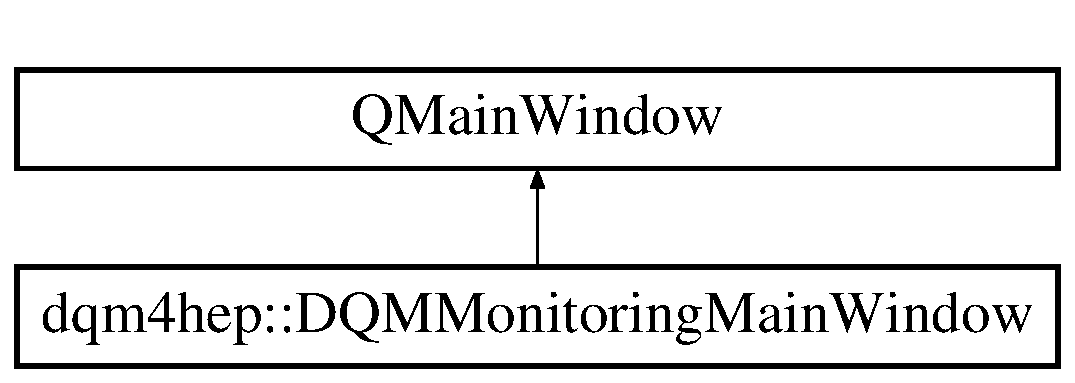
\includegraphics[height=2.000000cm]{classdqm4hep_1_1DQMMonitoringMainWindow}
\end{center}
\end{figure}
\subsection*{Public Member Functions}
\begin{DoxyCompactItemize}
\item 
{\bf D\+Q\+M\+Monitoring\+Main\+Window} ({\bf D\+Q\+M\+Monitoring} $\ast$p\+Monitoring)
\item 
void {\bf close\+Event} (Q\+Close\+Event $\ast$p\+Close\+Event)
\end{DoxyCompactItemize}
\subsection*{Private Attributes}
\begin{DoxyCompactItemize}
\item 
{\bf D\+Q\+M\+Monitoring} $\ast$ {\bf m\+\_\+p\+Monitoring}
\end{DoxyCompactItemize}


\subsection{Detailed Description}


Definition at line 60 of file D\+Q\+M\+Monitoring\+View.\+cc.



\subsection{Constructor \& Destructor Documentation}
\index{dqm4hep\+::\+D\+Q\+M\+Monitoring\+Main\+Window@{dqm4hep\+::\+D\+Q\+M\+Monitoring\+Main\+Window}!D\+Q\+M\+Monitoring\+Main\+Window@{D\+Q\+M\+Monitoring\+Main\+Window}}
\index{D\+Q\+M\+Monitoring\+Main\+Window@{D\+Q\+M\+Monitoring\+Main\+Window}!dqm4hep\+::\+D\+Q\+M\+Monitoring\+Main\+Window@{dqm4hep\+::\+D\+Q\+M\+Monitoring\+Main\+Window}}
\subsubsection[{D\+Q\+M\+Monitoring\+Main\+Window}]{\setlength{\rightskip}{0pt plus 5cm}dqm4hep\+::\+D\+Q\+M\+Monitoring\+Main\+Window\+::\+D\+Q\+M\+Monitoring\+Main\+Window (
\begin{DoxyParamCaption}
\item[{{\bf D\+Q\+M\+Monitoring} $\ast$}]{p\+Monitoring}
\end{DoxyParamCaption}
)\hspace{0.3cm}{\ttfamily [inline]}}\label{classdqm4hep_1_1DQMMonitoringMainWindow_aa591f6400ae7042da4b3b699863377ef}


Definition at line 63 of file D\+Q\+M\+Monitoring\+View.\+cc.


\begin{DoxyCode}
63                                                       :
64     m_pMonitoring(pMonitoring)
65   \{
66     \textcolor{comment}{/* nop */}
67   \}
\end{DoxyCode}


\subsection{Member Function Documentation}
\index{dqm4hep\+::\+D\+Q\+M\+Monitoring\+Main\+Window@{dqm4hep\+::\+D\+Q\+M\+Monitoring\+Main\+Window}!close\+Event@{close\+Event}}
\index{close\+Event@{close\+Event}!dqm4hep\+::\+D\+Q\+M\+Monitoring\+Main\+Window@{dqm4hep\+::\+D\+Q\+M\+Monitoring\+Main\+Window}}
\subsubsection[{close\+Event}]{\setlength{\rightskip}{0pt plus 5cm}void dqm4hep\+::\+D\+Q\+M\+Monitoring\+Main\+Window\+::close\+Event (
\begin{DoxyParamCaption}
\item[{Q\+Close\+Event $\ast$}]{p\+Close\+Event}
\end{DoxyParamCaption}
)\hspace{0.3cm}{\ttfamily [inline]}}\label{classdqm4hep_1_1DQMMonitoringMainWindow_a1be52d588370df6474e0e0c060110476}


Definition at line 69 of file D\+Q\+M\+Monitoring\+View.\+cc.



References dqm4hep\+::\+D\+Q\+M\+Monitoring\+::get\+Controller(), m\+\_\+p\+Monitoring, and dqm4hep\+::\+D\+Q\+M\+Monitoring\+Controller\+::quit().


\begin{DoxyCode}
70   \{
71     m_pMonitoring->getController()->quit();
72     pCloseEvent->accept();
73   \}
\end{DoxyCode}


\subsection{Member Data Documentation}
\index{dqm4hep\+::\+D\+Q\+M\+Monitoring\+Main\+Window@{dqm4hep\+::\+D\+Q\+M\+Monitoring\+Main\+Window}!m\+\_\+p\+Monitoring@{m\+\_\+p\+Monitoring}}
\index{m\+\_\+p\+Monitoring@{m\+\_\+p\+Monitoring}!dqm4hep\+::\+D\+Q\+M\+Monitoring\+Main\+Window@{dqm4hep\+::\+D\+Q\+M\+Monitoring\+Main\+Window}}
\subsubsection[{m\+\_\+p\+Monitoring}]{\setlength{\rightskip}{0pt plus 5cm}{\bf D\+Q\+M\+Monitoring}$\ast$ dqm4hep\+::\+D\+Q\+M\+Monitoring\+Main\+Window\+::m\+\_\+p\+Monitoring\hspace{0.3cm}{\ttfamily [private]}}\label{classdqm4hep_1_1DQMMonitoringMainWindow_a978cbf04dff7fbe59c865cbf533f09cf}


Definition at line 77 of file D\+Q\+M\+Monitoring\+View.\+cc.



Referenced by close\+Event().



The documentation for this class was generated from the following file\+:\begin{DoxyCompactItemize}
\item 
{\bf D\+Q\+M\+Monitoring\+View.\+cc}\end{DoxyCompactItemize}

\section{dqm4hep\+:\+:D\+Q\+M\+Monitoring\+Model Class Reference}
\label{classdqm4hep_1_1DQMMonitoringModel}\index{dqm4hep\+::\+D\+Q\+M\+Monitoring\+Model@{dqm4hep\+::\+D\+Q\+M\+Monitoring\+Model}}


\doxyref{D\+Q\+M\+Monitoring\+Model}{p.}{classdqm4hep_1_1DQMMonitoringModel} class.  




{\ttfamily \#include $<$D\+Q\+M\+Monitoring\+Model.\+h$>$}

Inheritance diagram for dqm4hep\+:\+:D\+Q\+M\+Monitoring\+Model\+:\begin{figure}[H]
\begin{center}
\leavevmode
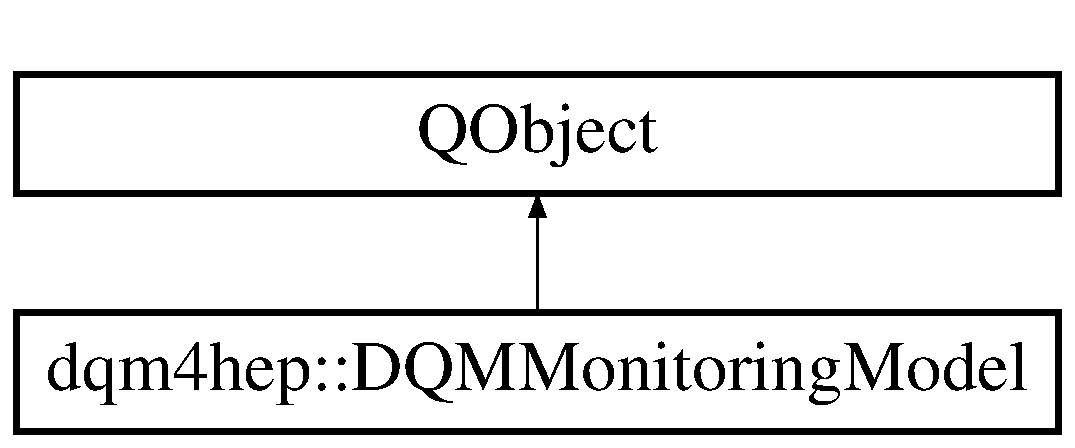
\includegraphics[height=2.000000cm]{classdqm4hep_1_1DQMMonitoringModel}
\end{center}
\end{figure}
\subsection*{Public Slots}
\begin{DoxyCompactItemize}
\item 
virtual void {\bf update\+Monitor\+Element} (D\+Q\+M\+Monitor\+Element $\ast$p\+Monitor\+Element)
\begin{DoxyCompactList}\small\item\em Update the monitor element in the model Add or replace if exists. \end{DoxyCompactList}\item 
virtual void {\bf update\+Monitor\+Element} ({\bf D\+Q\+M\+Gui\+Monitor\+Element} $\ast$p\+Monitor\+Element)
\begin{DoxyCompactList}\small\item\em Update the monitor element in the model Add or replace if exists. \end{DoxyCompactList}\item 
virtual void {\bf remove\+Monitor\+Element} ({\bf D\+Q\+M\+Gui\+Monitor\+Element} $\ast$p\+Monitor\+Element)
\begin{DoxyCompactList}\small\item\em Remove the monitor element form the model. \end{DoxyCompactList}\item 
void {\bf clear} ()
\begin{DoxyCompactList}\small\item\em Clear all the model contents. \end{DoxyCompactList}\item 
void {\bf clear} (const std\+::string \&collector\+Name)
\begin{DoxyCompactList}\small\item\em Clear all the elements of the given collector. \end{DoxyCompactList}\item 
void {\bf clear} (const std\+::string \&collector\+Name, const std\+::string \&module\+Name)
\begin{DoxyCompactList}\small\item\em Clear all the elements of the given collector and module. \end{DoxyCompactList}\end{DoxyCompactItemize}
\subsection*{Signals}
\begin{DoxyCompactItemize}
\item 
void {\bf monitor\+Element\+Added} ({\bf D\+Q\+M\+Gui\+Monitor\+Element} $\ast$p\+Monitor\+Element)
\begin{DoxyCompactList}\small\item\em Signal emitted when a monitor element is added to the model. \end{DoxyCompactList}\end{DoxyCompactItemize}
\subsection*{Public Member Functions}
\begin{DoxyCompactItemize}
\item 
{\bf D\+Q\+M\+Monitoring\+Model} ({\bf D\+Q\+M\+Monitoring} $\ast$p\+Monitoring)
\begin{DoxyCompactList}\small\item\em Constructor. \end{DoxyCompactList}\item 
virtual {\bf $\sim$\+D\+Q\+M\+Monitoring\+Model} ()
\begin{DoxyCompactList}\small\item\em Destructor. \end{DoxyCompactList}\item 
{\bf D\+Q\+M\+Monitoring} $\ast$ {\bf get\+Monitoring} () const 
\begin{DoxyCompactList}\small\item\em Get the monitoring instance. \end{DoxyCompactList}\item 
virtual bool {\bf monitor\+Element\+Exists} ({\bf D\+Q\+M\+Gui\+Monitor\+Element} $\ast$p\+Monitor\+Element) const 
\begin{DoxyCompactList}\small\item\em Whether the monitor element exists. \end{DoxyCompactList}\item 
virtual {\bf D\+Q\+M\+Gui\+Monitor\+Element} $\ast$ {\bf create\+Gui\+Monitor\+Element} (D\+Q\+M\+Monitor\+Element $\ast$p\+Monitor\+Element) const 
\begin{DoxyCompactList}\small\item\em Factory method that create a wrapper around a monitor element in the Qt framework. \end{DoxyCompactList}\item 
{\bf D\+Q\+M\+Gui\+Monitor\+Element} $\ast$ {\bf get\+Or\+Create\+Gui\+Monitor\+Element} (const std\+::string \&collector\+Name, const std\+::string \&module\+Name, const std\+::string \&full\+Path, const std\+::string \&name)
\item 
void {\bf load\+Monitor\+Element\+Info\+List} (const std\+::string \&collector\+Name, const D\+Q\+M\+Monitor\+Element\+Info\+List \&name\+List)
\item 
virtual {\bf D\+Q\+M\+Gui\+Monitor\+Element} $\ast$ {\bf create\+Gui\+Monitor\+Element} (const std\+::string \&collector\+Name, const std\+::string \&module\+Name, const std\+::string \&full\+Path, const std\+::string \&name) const 
\begin{DoxyCompactList}\small\item\em Factory method that create a wrapper around a monitor element in the Qt framework. \end{DoxyCompactList}\item 
virtual {\bf D\+Q\+M\+Gui\+Monitor\+Element} $\ast$ {\bf find\+Monitor\+Element} (const std\+::string \&collector\+Name, const std\+::string \&module\+Name, const std\+::string \&full\+Path, const std\+::string \&name) const 
\begin{DoxyCompactList}\small\item\em Find and return a monitor element identified by its collector name, module name, full path and name Return N\+U\+L\+L if not found. \end{DoxyCompactList}\end{DoxyCompactItemize}
\subsection*{Protected Attributes}
\begin{DoxyCompactItemize}
\item 
{\bf D\+Q\+M\+Monitoring} $\ast$ {\bf m\+\_\+p\+Monitoring}
\item 
{\bf D\+Q\+M\+Gui\+Monitor\+Element\+List} {\bf m\+\_\+monitor\+Element\+List}
\end{DoxyCompactItemize}
\subsection*{Private Types}
\begin{DoxyCompactItemize}
\item 
typedef std\+::vector\\*
$<$ {\bf D\+Q\+M\+Gui\+Monitor\+Element} $\ast$ $>$ {\bf D\+Q\+M\+Gui\+Monitor\+Element\+List}
\end{DoxyCompactItemize}


\subsection{Detailed Description}
\doxyref{D\+Q\+M\+Monitoring\+Model}{p.}{classdqm4hep_1_1DQMMonitoringModel} class. 

Definition at line 49 of file D\+Q\+M\+Monitoring\+Model.\+h.



\subsection{Member Typedef Documentation}
\index{dqm4hep\+::\+D\+Q\+M\+Monitoring\+Model@{dqm4hep\+::\+D\+Q\+M\+Monitoring\+Model}!D\+Q\+M\+Gui\+Monitor\+Element\+List@{D\+Q\+M\+Gui\+Monitor\+Element\+List}}
\index{D\+Q\+M\+Gui\+Monitor\+Element\+List@{D\+Q\+M\+Gui\+Monitor\+Element\+List}!dqm4hep\+::\+D\+Q\+M\+Monitoring\+Model@{dqm4hep\+::\+D\+Q\+M\+Monitoring\+Model}}
\subsubsection[{D\+Q\+M\+Gui\+Monitor\+Element\+List}]{\setlength{\rightskip}{0pt plus 5cm}typedef std\+::vector$<${\bf D\+Q\+M\+Gui\+Monitor\+Element}$\ast$$>$ {\bf dqm4hep\+::\+D\+Q\+M\+Monitoring\+Model\+::\+D\+Q\+M\+Gui\+Monitor\+Element\+List}\hspace{0.3cm}{\ttfamily [private]}}\label{classdqm4hep_1_1DQMMonitoringModel_a34f4be1cc55e10b7dc4efe686faaea5e}


Definition at line 53 of file D\+Q\+M\+Monitoring\+Model.\+h.



\subsection{Constructor \& Destructor Documentation}
\index{dqm4hep\+::\+D\+Q\+M\+Monitoring\+Model@{dqm4hep\+::\+D\+Q\+M\+Monitoring\+Model}!D\+Q\+M\+Monitoring\+Model@{D\+Q\+M\+Monitoring\+Model}}
\index{D\+Q\+M\+Monitoring\+Model@{D\+Q\+M\+Monitoring\+Model}!dqm4hep\+::\+D\+Q\+M\+Monitoring\+Model@{dqm4hep\+::\+D\+Q\+M\+Monitoring\+Model}}
\subsubsection[{D\+Q\+M\+Monitoring\+Model}]{\setlength{\rightskip}{0pt plus 5cm}dqm4hep\+::\+D\+Q\+M\+Monitoring\+Model\+::\+D\+Q\+M\+Monitoring\+Model (
\begin{DoxyParamCaption}
\item[{{\bf D\+Q\+M\+Monitoring} $\ast$}]{p\+Monitoring}
\end{DoxyParamCaption}
)}\label{classdqm4hep_1_1DQMMonitoringModel_a464b71d31d373c237775d6548a7d3c3f}


Constructor. 



Definition at line 46 of file D\+Q\+M\+Monitoring\+Model.\+cc.



References m\+\_\+p\+Monitoring, and dqm4hep\+::\+D\+Q\+M\+Monitoring\+::set\+Model().


\begin{DoxyCode}
46                                                                  :
47     m_pMonitoring(pMonitoring)
48 \{
49   m_pMonitoring->setModel(\textcolor{keyword}{this});
50 \}
\end{DoxyCode}
\index{dqm4hep\+::\+D\+Q\+M\+Monitoring\+Model@{dqm4hep\+::\+D\+Q\+M\+Monitoring\+Model}!````~D\+Q\+M\+Monitoring\+Model@{$\sim$\+D\+Q\+M\+Monitoring\+Model}}
\index{````~D\+Q\+M\+Monitoring\+Model@{$\sim$\+D\+Q\+M\+Monitoring\+Model}!dqm4hep\+::\+D\+Q\+M\+Monitoring\+Model@{dqm4hep\+::\+D\+Q\+M\+Monitoring\+Model}}
\subsubsection[{$\sim$\+D\+Q\+M\+Monitoring\+Model}]{\setlength{\rightskip}{0pt plus 5cm}dqm4hep\+::\+D\+Q\+M\+Monitoring\+Model\+::$\sim$\+D\+Q\+M\+Monitoring\+Model (
\begin{DoxyParamCaption}
{}
\end{DoxyParamCaption}
)\hspace{0.3cm}{\ttfamily [virtual]}}\label{classdqm4hep_1_1DQMMonitoringModel_a773c12bea89eb345bc42ecac64cbbab7}


Destructor. 



Definition at line 54 of file D\+Q\+M\+Monitoring\+Model.\+cc.



References clear().


\begin{DoxyCode}
55 \{
56   clear();
57 \}
\end{DoxyCode}


\subsection{Member Function Documentation}
\index{dqm4hep\+::\+D\+Q\+M\+Monitoring\+Model@{dqm4hep\+::\+D\+Q\+M\+Monitoring\+Model}!clear@{clear}}
\index{clear@{clear}!dqm4hep\+::\+D\+Q\+M\+Monitoring\+Model@{dqm4hep\+::\+D\+Q\+M\+Monitoring\+Model}}
\subsubsection[{clear}]{\setlength{\rightskip}{0pt plus 5cm}void dqm4hep\+::\+D\+Q\+M\+Monitoring\+Model\+::clear (
\begin{DoxyParamCaption}
{}
\end{DoxyParamCaption}
)\hspace{0.3cm}{\ttfamily [slot]}}\label{classdqm4hep_1_1DQMMonitoringModel_ae30dc0d2d219ae200ee42fff9d553b04}


Clear all the model contents. 



Definition at line 157 of file D\+Q\+M\+Monitoring\+Model.\+cc.



References dqm4hep\+::\+D\+Q\+M\+Monitoring\+View\+::get\+Monitor\+Element\+View(), get\+Monitoring(), dqm4hep\+::\+D\+Q\+M\+Monitoring\+::get\+View(), m\+\_\+monitor\+Element\+List, and dqm4hep\+::\+D\+Q\+M\+Monitor\+Element\+View\+::remove\+Monitor\+Element().



Referenced by dqm4hep\+::\+D\+Q\+M\+Monitoring\+Controller\+::clear\+Monitoring(), dqm4hep\+::\+D\+Q\+M\+Monitoring\+Controller\+::clear\+View\+And\+Model(), dqm4hep\+::\+D\+Q\+M\+Monitoring\+Controller\+::open\+File(), and $\sim$\+D\+Q\+M\+Monitoring\+Model().


\begin{DoxyCode}
158 \{
159   \textcolor{keywordflow}{for}(DQMGuiMonitorElementList::iterator iter = m_monitorElementList.begin(), endIter = 
      m_monitorElementList.end() ;
160       endIter != iter ; ++iter)
161   \{
162     DQMGuiMonitorElement *pGuiMonitorElement = *iter;
163 
164     this->getMonitoring()->getView()->getMonitorElementView()->
      removeMonitorElement(pGuiMonitorElement);
165     pGuiMonitorElement->deleteLater();
166   \}
167 
168   m_monitorElementList.clear();
169 \}
\end{DoxyCode}
\index{dqm4hep\+::\+D\+Q\+M\+Monitoring\+Model@{dqm4hep\+::\+D\+Q\+M\+Monitoring\+Model}!clear@{clear}}
\index{clear@{clear}!dqm4hep\+::\+D\+Q\+M\+Monitoring\+Model@{dqm4hep\+::\+D\+Q\+M\+Monitoring\+Model}}
\subsubsection[{clear}]{\setlength{\rightskip}{0pt plus 5cm}void dqm4hep\+::\+D\+Q\+M\+Monitoring\+Model\+::clear (
\begin{DoxyParamCaption}
\item[{const std\+::string \&}]{collector\+Name}
\end{DoxyParamCaption}
)\hspace{0.3cm}{\ttfamily [slot]}}\label{classdqm4hep_1_1DQMMonitoringModel_af5b50ce27e3426f06f079ff9cc91c27f}


Clear all the elements of the given collector. 



Definition at line 173 of file D\+Q\+M\+Monitoring\+Model.\+cc.



References dqm4hep\+::\+D\+Q\+M\+Monitoring\+View\+::get\+Monitor\+Element\+View(), get\+Monitoring(), dqm4hep\+::\+D\+Q\+M\+Monitoring\+::get\+View(), m\+\_\+monitor\+Element\+List, and dqm4hep\+::\+D\+Q\+M\+Monitor\+Element\+View\+::remove\+Monitor\+Element().


\begin{DoxyCode}
174 \{
175   \textcolor{keywordflow}{for}(DQMGuiMonitorElementList::iterator iter = m_monitorElementList.begin(), endIter = 
      m_monitorElementList.end() ;
176       endIter != iter ; ++iter)
177   \{
178     \textcolor{keyword}{const} std::string &thisCollectorName = (*iter)->getMonitorElement()->getCollectorName();
179 
180     \textcolor{keywordflow}{if}(thisCollectorName == collectorName)
181     \{
182       DQMGuiMonitorElement *pGuiMonitorElement = *iter;
183 
184       \textcolor{comment}{// remove it}
185       m_monitorElementList.erase(iter);
186       iter--;
187 
188       \textcolor{comment}{// notify view}
189       this->getMonitoring()->getView()->getMonitorElementView()->
      removeMonitorElement(pGuiMonitorElement);
190 
191       \textcolor{comment}{// delete it}
192       pGuiMonitorElement->deleteLater();
193     \}
194   \}
195 \}
\end{DoxyCode}
\index{dqm4hep\+::\+D\+Q\+M\+Monitoring\+Model@{dqm4hep\+::\+D\+Q\+M\+Monitoring\+Model}!clear@{clear}}
\index{clear@{clear}!dqm4hep\+::\+D\+Q\+M\+Monitoring\+Model@{dqm4hep\+::\+D\+Q\+M\+Monitoring\+Model}}
\subsubsection[{clear}]{\setlength{\rightskip}{0pt plus 5cm}void dqm4hep\+::\+D\+Q\+M\+Monitoring\+Model\+::clear (
\begin{DoxyParamCaption}
\item[{const std\+::string \&}]{collector\+Name, }
\item[{const std\+::string \&}]{module\+Name}
\end{DoxyParamCaption}
)\hspace{0.3cm}{\ttfamily [slot]}}\label{classdqm4hep_1_1DQMMonitoringModel_a467e6737e4b2aeebdef93ad7b9b2414e}


Clear all the elements of the given collector and module. 



Definition at line 199 of file D\+Q\+M\+Monitoring\+Model.\+cc.



References dqm4hep\+::\+D\+Q\+M\+Monitoring\+View\+::get\+Monitor\+Element\+View(), get\+Monitoring(), dqm4hep\+::\+D\+Q\+M\+Monitoring\+::get\+View(), m\+\_\+monitor\+Element\+List, and dqm4hep\+::\+D\+Q\+M\+Monitor\+Element\+View\+::remove\+Monitor\+Element().


\begin{DoxyCode}
200 \{
201   \textcolor{keywordflow}{for}(DQMGuiMonitorElementList::iterator iter = m_monitorElementList.begin(), endIter = 
      m_monitorElementList.end() ;
202       endIter != iter ; ++iter)
203   \{
204     \textcolor{keyword}{const} std::string &thisCollectorName = (*iter)->getMonitorElement()->getCollectorName();
205     \textcolor{keyword}{const} std::string &thisModuleName = (*iter)->getMonitorElement()->getModuleName();
206 
207     \textcolor{keywordflow}{if}(thisCollectorName == collectorName && thisModuleName == moduleName)
208     \{
209       DQMGuiMonitorElement *pGuiMonitorElement = *iter;
210 
211       \textcolor{comment}{// remove it}
212       m_monitorElementList.erase(iter);
213       iter--;
214 
215       \textcolor{comment}{// notify view}
216       this->getMonitoring()->getView()->getMonitorElementView()->
      removeMonitorElement(pGuiMonitorElement);
217 
218       \textcolor{comment}{// delete it}
219       pGuiMonitorElement->deleteLater();
220     \}
221   \}
222 \}
\end{DoxyCode}
\index{dqm4hep\+::\+D\+Q\+M\+Monitoring\+Model@{dqm4hep\+::\+D\+Q\+M\+Monitoring\+Model}!create\+Gui\+Monitor\+Element@{create\+Gui\+Monitor\+Element}}
\index{create\+Gui\+Monitor\+Element@{create\+Gui\+Monitor\+Element}!dqm4hep\+::\+D\+Q\+M\+Monitoring\+Model@{dqm4hep\+::\+D\+Q\+M\+Monitoring\+Model}}
\subsubsection[{create\+Gui\+Monitor\+Element}]{\setlength{\rightskip}{0pt plus 5cm}{\bf D\+Q\+M\+Gui\+Monitor\+Element} $\ast$ dqm4hep\+::\+D\+Q\+M\+Monitoring\+Model\+::create\+Gui\+Monitor\+Element (
\begin{DoxyParamCaption}
\item[{D\+Q\+M\+Monitor\+Element $\ast$}]{p\+Monitor\+Element}
\end{DoxyParamCaption}
) const\hspace{0.3cm}{\ttfamily [virtual]}}\label{classdqm4hep_1_1DQMMonitoringModel_ab1baa2e84f12a9c716bdefc85a3b2e76}


Factory method that create a wrapper around a monitor element in the Qt framework. 

The created monitor element is not registered in the model. Use update\+Monitor\+Element(elt) to register it 

Definition at line 243 of file D\+Q\+M\+Monitoring\+Model.\+cc.



Referenced by create\+Gui\+Monitor\+Element(), dqm4hep\+::\+D\+Q\+M\+Canvas\+View\+::from\+Xml(), get\+Or\+Create\+Gui\+Monitor\+Element(), load\+Monitor\+Element\+Info\+List(), and update\+Monitor\+Element().


\begin{DoxyCode}
244 \{
245   \textcolor{keywordflow}{if}(!pMonitorElement)
246     \textcolor{keywordflow}{return} NULL;
247 
248   DQMGuiMonitorElement *pGuiMonitorElement = \textcolor{keyword}{new} DQMGuiMonitorElement(pMonitorElement);
249 
250   \textcolor{keywordflow}{return} pGuiMonitorElement;
251 \}
\end{DoxyCode}
\index{dqm4hep\+::\+D\+Q\+M\+Monitoring\+Model@{dqm4hep\+::\+D\+Q\+M\+Monitoring\+Model}!create\+Gui\+Monitor\+Element@{create\+Gui\+Monitor\+Element}}
\index{create\+Gui\+Monitor\+Element@{create\+Gui\+Monitor\+Element}!dqm4hep\+::\+D\+Q\+M\+Monitoring\+Model@{dqm4hep\+::\+D\+Q\+M\+Monitoring\+Model}}
\subsubsection[{create\+Gui\+Monitor\+Element}]{\setlength{\rightskip}{0pt plus 5cm}{\bf D\+Q\+M\+Gui\+Monitor\+Element} $\ast$ dqm4hep\+::\+D\+Q\+M\+Monitoring\+Model\+::create\+Gui\+Monitor\+Element (
\begin{DoxyParamCaption}
\item[{const std\+::string \&}]{collector\+Name, }
\item[{const std\+::string \&}]{module\+Name, }
\item[{const std\+::string \&}]{full\+Path, }
\item[{const std\+::string \&}]{name}
\end{DoxyParamCaption}
) const\hspace{0.3cm}{\ttfamily [virtual]}}\label{classdqm4hep_1_1DQMMonitoringModel_a06da7b1b7bb100724462d214d619d658}


Factory method that create a wrapper around a monitor element in the Qt framework. 

The created monitor element is not registered in the model. Use update\+Monitor\+Element(elt) to register it 

Definition at line 345 of file D\+Q\+M\+Monitoring\+Model.\+cc.



References create\+Gui\+Monitor\+Element().


\begin{DoxyCode}
347 \{
348   DQMMonitorElement *pMonitorElement = \textcolor{keyword}{new} DQMMonitorElement(NO\_ELEMENT\_TYPE, name, \textcolor{stringliteral}{""}, moduleName);
349   pMonitorElement->setCollectorName(collectorName);
350   pMonitorElement->setPath(DQMPath(fullPath));
351 
352   \textcolor{keywordflow}{return} this->createGuiMonitorElement(pMonitorElement);
353 \}
\end{DoxyCode}
\index{dqm4hep\+::\+D\+Q\+M\+Monitoring\+Model@{dqm4hep\+::\+D\+Q\+M\+Monitoring\+Model}!find\+Monitor\+Element@{find\+Monitor\+Element}}
\index{find\+Monitor\+Element@{find\+Monitor\+Element}!dqm4hep\+::\+D\+Q\+M\+Monitoring\+Model@{dqm4hep\+::\+D\+Q\+M\+Monitoring\+Model}}
\subsubsection[{find\+Monitor\+Element}]{\setlength{\rightskip}{0pt plus 5cm}{\bf D\+Q\+M\+Gui\+Monitor\+Element} $\ast$ dqm4hep\+::\+D\+Q\+M\+Monitoring\+Model\+::find\+Monitor\+Element (
\begin{DoxyParamCaption}
\item[{const std\+::string \&}]{collector\+Name, }
\item[{const std\+::string \&}]{module\+Name, }
\item[{const std\+::string \&}]{full\+Path, }
\item[{const std\+::string \&}]{name}
\end{DoxyParamCaption}
) const\hspace{0.3cm}{\ttfamily [virtual]}}\label{classdqm4hep_1_1DQMMonitoringModel_ae93da158dd3698dd33822960ad516b4d}


Find and return a monitor element identified by its collector name, module name, full path and name Return N\+U\+L\+L if not found. 



Definition at line 357 of file D\+Q\+M\+Monitoring\+Model.\+cc.



References dqm4hep\+::\+D\+Q\+M\+Gui\+Monitor\+Element\+::get\+Monitor\+Element(), and m\+\_\+monitor\+Element\+List.



Referenced by dqm4hep\+::\+D\+Q\+M\+Monitor\+Element\+Navigator\+::draw\+Selected\+Monitor\+Elements(), dqm4hep\+::\+D\+Q\+M\+Canvas\+Area\+::drop\+Event(), dqm4hep\+::\+D\+Q\+M\+Canvas\+View\+::from\+Xml(), dqm4hep\+::\+D\+Q\+M\+Monitor\+Element\+Navigator\+::handle\+Item\+Double\+Click(), dqm4hep\+::\+D\+Q\+M\+Monitor\+Element\+Navigator\+::key\+Press\+Event(), dqm4hep\+::\+D\+Q\+M\+Monitor\+Element\+Navigator\+::query\+Update(), and update\+Monitor\+Element().


\begin{DoxyCode}
359 \{
360   DQMPath path = fullPath;
361 
362   \textcolor{keywordflow}{for}(DQMGuiMonitorElementList::const\_iterator iter = m_monitorElementList.begin(), endIter = 
      m_monitorElementList.end() ;
363       endIter != iter ; ++iter)
364   \{
365     \textcolor{keyword}{const} std::string &meCollectorName = (*iter)->getMonitorElement()->getCollectorName();
366     \textcolor{keyword}{const} DQMPath     &mePath = (*iter)->getMonitorElement()->getPath();
367     \textcolor{keyword}{const} std::string &meModuleName = (*iter)->getMonitorElement()->getModuleName();
368     \textcolor{keyword}{const} std::string &meName = (*iter)->getMonitorElement()->getName();
369 
370     \textcolor{keywordtype}{bool} sameCollectorName = (collectorName == meCollectorName);
371     \textcolor{keywordtype}{bool} samePath =          (path          == mePath);
372     \textcolor{keywordtype}{bool} sameModuleName =    (moduleName    == meModuleName);
373     \textcolor{keywordtype}{bool} sameName =          (name          == meName);
374 
375     \textcolor{keywordflow}{if}(sameCollectorName && samePath && sameModuleName && sameName)
376     \{
377       \textcolor{keywordflow}{return} (*iter);
378     \}
379   \}
380 
381   \textcolor{keywordflow}{return} NULL;
382 \}
\end{DoxyCode}
\index{dqm4hep\+::\+D\+Q\+M\+Monitoring\+Model@{dqm4hep\+::\+D\+Q\+M\+Monitoring\+Model}!get\+Monitoring@{get\+Monitoring}}
\index{get\+Monitoring@{get\+Monitoring}!dqm4hep\+::\+D\+Q\+M\+Monitoring\+Model@{dqm4hep\+::\+D\+Q\+M\+Monitoring\+Model}}
\subsubsection[{get\+Monitoring}]{\setlength{\rightskip}{0pt plus 5cm}{\bf D\+Q\+M\+Monitoring} $\ast$ dqm4hep\+::\+D\+Q\+M\+Monitoring\+Model\+::get\+Monitoring (
\begin{DoxyParamCaption}
{}
\end{DoxyParamCaption}
) const}\label{classdqm4hep_1_1DQMMonitoringModel_ac68b20698825b43377d1fb68913721e0}


Get the monitoring instance. 



Definition at line 61 of file D\+Q\+M\+Monitoring\+Model.\+cc.



References m\+\_\+p\+Monitoring.



Referenced by clear(), get\+Or\+Create\+Gui\+Monitor\+Element(), load\+Monitor\+Element\+Info\+List(), remove\+Monitor\+Element(), and update\+Monitor\+Element().


\begin{DoxyCode}
62 \{
63   \textcolor{keywordflow}{return} m_pMonitoring;
64 \}
\end{DoxyCode}
\index{dqm4hep\+::\+D\+Q\+M\+Monitoring\+Model@{dqm4hep\+::\+D\+Q\+M\+Monitoring\+Model}!get\+Or\+Create\+Gui\+Monitor\+Element@{get\+Or\+Create\+Gui\+Monitor\+Element}}
\index{get\+Or\+Create\+Gui\+Monitor\+Element@{get\+Or\+Create\+Gui\+Monitor\+Element}!dqm4hep\+::\+D\+Q\+M\+Monitoring\+Model@{dqm4hep\+::\+D\+Q\+M\+Monitoring\+Model}}
\subsubsection[{get\+Or\+Create\+Gui\+Monitor\+Element}]{\setlength{\rightskip}{0pt plus 5cm}{\bf D\+Q\+M\+Gui\+Monitor\+Element} $\ast$ dqm4hep\+::\+D\+Q\+M\+Monitoring\+Model\+::get\+Or\+Create\+Gui\+Monitor\+Element (
\begin{DoxyParamCaption}
\item[{const std\+::string \&}]{collector\+Name, }
\item[{const std\+::string \&}]{module\+Name, }
\item[{const std\+::string \&}]{full\+Path, }
\item[{const std\+::string \&}]{name}
\end{DoxyParamCaption}
)}\label{classdqm4hep_1_1DQMMonitoringModel_ad52b8ba5826c8da15f71d967ad2bd593}


Definition at line 255 of file D\+Q\+M\+Monitoring\+Model.\+cc.



References dqm4hep\+::\+D\+Q\+M\+Monitor\+Element\+View\+::add\+Monitor\+Element(), create\+Gui\+Monitor\+Element(), dqm4hep\+::\+D\+Q\+M\+Gui\+Monitor\+Element\+::get\+Monitor\+Element(), dqm4hep\+::\+D\+Q\+M\+Monitoring\+View\+::get\+Monitor\+Element\+View(), get\+Monitoring(), dqm4hep\+::\+D\+Q\+M\+Monitoring\+::get\+View(), and m\+\_\+monitor\+Element\+List.


\begin{DoxyCode}
257 \{
258   DQMPath path = fullPath;
259   DQMGuiMonitorElement *pMonitorElement = NULL;
260 
261   \textcolor{keywordflow}{for}(DQMGuiMonitorElementList::const\_iterator iter = m_monitorElementList.begin(), endIter = 
      m_monitorElementList.end() ;
262       endIter != iter ; ++iter)
263   \{
264     \textcolor{keyword}{const} std::string &meCollectorName = (*iter)->getMonitorElement()->getCollectorName();
265     \textcolor{keyword}{const} DQMPath     &mePath = (*iter)->getMonitorElement()->getPath();
266     \textcolor{keyword}{const} std::string &meModuleName = (*iter)->getMonitorElement()->getModuleName();
267     \textcolor{keyword}{const} std::string &meName = (*iter)->getMonitorElement()->getName();
268 
269     \textcolor{keywordtype}{bool} sameCollectorName = (collectorName == meCollectorName);
270     \textcolor{keywordtype}{bool} samePath =          (path          == mePath);
271     \textcolor{keywordtype}{bool} sameModuleName =    (moduleName    == meModuleName);
272     \textcolor{keywordtype}{bool} sameName =          (name          == meName);
273 
274     \textcolor{keywordflow}{if}(sameCollectorName && samePath && sameModuleName && sameName)
275     \{
276       pMonitorElement = (*iter);
277       \textcolor{keywordflow}{break};
278     \}
279   \}
280 
281   \textcolor{keywordflow}{if}(NULL == pMonitorElement)
282   \{
283     pMonitorElement = this->createGuiMonitorElement(collectorName, moduleName, fullPath, name);
284 
285     \textcolor{comment}{// register it}
286     m_monitorElementList.push\_back(pMonitorElement);
287 
288     \textcolor{comment}{// notify view}
289     this->getMonitoring()->getView()->getMonitorElementView()->addMonitorElement(pMonitorElement);
290   \}
291 
292   \textcolor{keywordflow}{return} pMonitorElement;
293 \}
\end{DoxyCode}
\index{dqm4hep\+::\+D\+Q\+M\+Monitoring\+Model@{dqm4hep\+::\+D\+Q\+M\+Monitoring\+Model}!load\+Monitor\+Element\+Info\+List@{load\+Monitor\+Element\+Info\+List}}
\index{load\+Monitor\+Element\+Info\+List@{load\+Monitor\+Element\+Info\+List}!dqm4hep\+::\+D\+Q\+M\+Monitoring\+Model@{dqm4hep\+::\+D\+Q\+M\+Monitoring\+Model}}
\subsubsection[{load\+Monitor\+Element\+Info\+List}]{\setlength{\rightskip}{0pt plus 5cm}void dqm4hep\+::\+D\+Q\+M\+Monitoring\+Model\+::load\+Monitor\+Element\+Info\+List (
\begin{DoxyParamCaption}
\item[{const std\+::string \&}]{collector\+Name, }
\item[{const D\+Q\+M\+Monitor\+Element\+Info\+List \&}]{name\+List}
\end{DoxyParamCaption}
)}\label{classdqm4hep_1_1DQMMonitoringModel_a4a50a519fb773147194f01cfd2d288b7}


Definition at line 297 of file D\+Q\+M\+Monitoring\+Model.\+cc.



References dqm4hep\+::\+D\+Q\+M\+Monitor\+Element\+View\+::add\+Monitor\+Element(), create\+Gui\+Monitor\+Element(), dqm4hep\+::\+D\+Q\+M\+Gui\+Monitor\+Element\+::get\+Monitor\+Element(), dqm4hep\+::\+D\+Q\+M\+Monitoring\+View\+::get\+Monitor\+Element\+View(), get\+Monitoring(), dqm4hep\+::\+D\+Q\+M\+Monitoring\+::get\+View(), and m\+\_\+monitor\+Element\+List.



Referenced by dqm4hep\+::\+D\+Q\+M\+Monitoring\+Controller\+::create\+Empty\+Monitor\+Elements().


\begin{DoxyCode}
298 \{
299   DQMGuiMonitorElementList addedMonitorElement;
300 
301   \textcolor{keywordflow}{for}(DQMMonitorElementInfoList::const\_iterator meIter = nameList.begin(), meEndIter = nameList.end() ;
302       meEndIter != meIter ; ++meIter)
303   \{
304     DQMPath path = meIter->m\_monitorElementFullPath;
305     DQMGuiMonitorElement *pMonitorElement = NULL;
306 
307     \textcolor{keywordflow}{for}(DQMGuiMonitorElementList::const\_iterator iter = m_monitorElementList.begin(), endIter = 
      m_monitorElementList.end() ;
308         endIter != iter ; ++iter)
309     \{
310       \textcolor{keyword}{const} std::string &meCollectorName = (*iter)->getMonitorElement()->getCollectorName();
311       \textcolor{keyword}{const} DQMPath     &mePath = (*iter)->getMonitorElement()->getPath();
312       \textcolor{keyword}{const} std::string &meModuleName = (*iter)->getMonitorElement()->getModuleName();
313       \textcolor{keyword}{const} std::string &meName = (*iter)->getMonitorElement()->getName();
314 
315       \textcolor{keywordtype}{bool} sameCollectorName = (collectorName == meCollectorName);
316       \textcolor{keywordtype}{bool} samePath =          (path          == mePath);
317       \textcolor{keywordtype}{bool} sameModuleName =    (meIter->m\_moduleName    == meModuleName);
318       \textcolor{keywordtype}{bool} sameName =          (meIter->m\_monitorElementName          == meName);
319 
320       \textcolor{keywordflow}{if}(sameCollectorName && samePath && sameModuleName && sameName)
321       \{
322         pMonitorElement = (*iter);
323         \textcolor{keywordflow}{break};
324       \}
325     \}
326 
327     \textcolor{keywordflow}{if}(NULL == pMonitorElement)
328     \{
329       pMonitorElement = this->createGuiMonitorElement(collectorName, meIter->m\_moduleName, meIter->
      m\_monitorElementFullPath, meIter->m\_monitorElementName);
330 
331       \textcolor{comment}{// add it to tmp list}
332       addedMonitorElement.push\_back(pMonitorElement);
333 
334       \textcolor{comment}{// notify view}
335       this->getMonitoring()->getView()->getMonitorElementView()->
      addMonitorElement(pMonitorElement);
336     \}
337   \}
338 
339   \textcolor{comment}{// register new content !}
340   m_monitorElementList.insert(m_monitorElementList.end(), addedMonitorElement.begin(), addedMonitorElement.
      end());
341 \}
\end{DoxyCode}
\index{dqm4hep\+::\+D\+Q\+M\+Monitoring\+Model@{dqm4hep\+::\+D\+Q\+M\+Monitoring\+Model}!monitor\+Element\+Added@{monitor\+Element\+Added}}
\index{monitor\+Element\+Added@{monitor\+Element\+Added}!dqm4hep\+::\+D\+Q\+M\+Monitoring\+Model@{dqm4hep\+::\+D\+Q\+M\+Monitoring\+Model}}
\subsubsection[{monitor\+Element\+Added}]{\setlength{\rightskip}{0pt plus 5cm}void dqm4hep\+::\+D\+Q\+M\+Monitoring\+Model\+::monitor\+Element\+Added (
\begin{DoxyParamCaption}
\item[{{\bf D\+Q\+M\+Gui\+Monitor\+Element} $\ast$}]{p\+Monitor\+Element}
\end{DoxyParamCaption}
)\hspace{0.3cm}{\ttfamily [signal]}}\label{classdqm4hep_1_1DQMMonitoringModel_a14f86c5869962643051c99f029f0e10d}


Signal emitted when a monitor element is added to the model. 

\index{dqm4hep\+::\+D\+Q\+M\+Monitoring\+Model@{dqm4hep\+::\+D\+Q\+M\+Monitoring\+Model}!monitor\+Element\+Exists@{monitor\+Element\+Exists}}
\index{monitor\+Element\+Exists@{monitor\+Element\+Exists}!dqm4hep\+::\+D\+Q\+M\+Monitoring\+Model@{dqm4hep\+::\+D\+Q\+M\+Monitoring\+Model}}
\subsubsection[{monitor\+Element\+Exists}]{\setlength{\rightskip}{0pt plus 5cm}bool dqm4hep\+::\+D\+Q\+M\+Monitoring\+Model\+::monitor\+Element\+Exists (
\begin{DoxyParamCaption}
\item[{{\bf D\+Q\+M\+Gui\+Monitor\+Element} $\ast$}]{p\+Monitor\+Element}
\end{DoxyParamCaption}
) const\hspace{0.3cm}{\ttfamily [virtual]}}\label{classdqm4hep_1_1DQMMonitoringModel_a188d7b9caf13b83295044552fa6e8ac4}


Whether the monitor element exists. 



Definition at line 226 of file D\+Q\+M\+Monitoring\+Model.\+cc.



References m\+\_\+monitor\+Element\+List.


\begin{DoxyCode}
227 \{
228   \textcolor{keywordflow}{if}(!pMonitorElement)
229     \textcolor{keywordflow}{return} \textcolor{keyword}{false};
230 
231   \textcolor{keywordflow}{for}(DQMGuiMonitorElementList::const\_iterator iter = m_monitorElementList.begin(), endIter = 
      m_monitorElementList.end() ;
232       endIter != iter ; ++iter)
233   \{
234     \textcolor{keywordflow}{if}((*iter)->equals(pMonitorElement))
235       \textcolor{keywordflow}{return} \textcolor{keyword}{true};
236   \}
237 
238   \textcolor{keywordflow}{return} \textcolor{keyword}{false};
239 \}
\end{DoxyCode}
\index{dqm4hep\+::\+D\+Q\+M\+Monitoring\+Model@{dqm4hep\+::\+D\+Q\+M\+Monitoring\+Model}!remove\+Monitor\+Element@{remove\+Monitor\+Element}}
\index{remove\+Monitor\+Element@{remove\+Monitor\+Element}!dqm4hep\+::\+D\+Q\+M\+Monitoring\+Model@{dqm4hep\+::\+D\+Q\+M\+Monitoring\+Model}}
\subsubsection[{remove\+Monitor\+Element}]{\setlength{\rightskip}{0pt plus 5cm}void dqm4hep\+::\+D\+Q\+M\+Monitoring\+Model\+::remove\+Monitor\+Element (
\begin{DoxyParamCaption}
\item[{{\bf D\+Q\+M\+Gui\+Monitor\+Element} $\ast$}]{p\+Monitor\+Element}
\end{DoxyParamCaption}
)\hspace{0.3cm}{\ttfamily [virtual]}, {\ttfamily [slot]}}\label{classdqm4hep_1_1DQMMonitoringModel_a8a238092bdf6e9c9e3ab6d99712505e3}


Remove the monitor element form the model. 



Definition at line 130 of file D\+Q\+M\+Monitoring\+Model.\+cc.



References dqm4hep\+::\+D\+Q\+M\+Monitoring\+View\+::get\+Monitor\+Element\+View(), get\+Monitoring(), dqm4hep\+::\+D\+Q\+M\+Monitoring\+::get\+View(), m\+\_\+monitor\+Element\+List, and dqm4hep\+::\+D\+Q\+M\+Monitor\+Element\+View\+::remove\+Monitor\+Element().


\begin{DoxyCode}
131 \{
132   \textcolor{keywordflow}{if}(!pMonitorElement)
133     \textcolor{keywordflow}{return};
134 
135   \textcolor{keywordflow}{for}(DQMGuiMonitorElementList::iterator iter = m_monitorElementList.begin(), endIter = 
      m_monitorElementList.end() ;
136       endIter != iter ; ++iter)
137   \{
138     DQMGuiMonitorElement *pGuiMonitorElement = *iter;
139 
140     \textcolor{keywordflow}{if}((*iter)->equals(pMonitorElement))
141     \{
142       \textcolor{comment}{// remove it}
143       m_monitorElementList.erase(iter);
144 
145       \textcolor{comment}{// notify view}
146       this->getMonitoring()->getView()->getMonitorElementView()->
      removeMonitorElement(pGuiMonitorElement);
147 
148       \textcolor{keywordflow}{break};
149     \}
150   \}
151 
152   pMonitorElement->deleteLater();
153 \}
\end{DoxyCode}
\index{dqm4hep\+::\+D\+Q\+M\+Monitoring\+Model@{dqm4hep\+::\+D\+Q\+M\+Monitoring\+Model}!update\+Monitor\+Element@{update\+Monitor\+Element}}
\index{update\+Monitor\+Element@{update\+Monitor\+Element}!dqm4hep\+::\+D\+Q\+M\+Monitoring\+Model@{dqm4hep\+::\+D\+Q\+M\+Monitoring\+Model}}
\subsubsection[{update\+Monitor\+Element}]{\setlength{\rightskip}{0pt plus 5cm}void dqm4hep\+::\+D\+Q\+M\+Monitoring\+Model\+::update\+Monitor\+Element (
\begin{DoxyParamCaption}
\item[{D\+Q\+M\+Monitor\+Element $\ast$}]{p\+Monitor\+Element}
\end{DoxyParamCaption}
)\hspace{0.3cm}{\ttfamily [virtual]}, {\ttfamily [slot]}}\label{classdqm4hep_1_1DQMMonitoringModel_a87e27408e938d2297a9de8a57210a991}


Update the monitor element in the model Add or replace if exists. 



Definition at line 68 of file D\+Q\+M\+Monitoring\+Model.\+cc.



References dqm4hep\+::\+D\+Q\+M\+Monitor\+Element\+View\+::add\+Monitor\+Element(), create\+Gui\+Monitor\+Element(), dqm4hep\+::\+D\+Q\+M\+Monitoring\+View\+::get\+Monitor\+Element\+View(), get\+Monitoring(), dqm4hep\+::\+D\+Q\+M\+Monitoring\+::get\+View(), m\+\_\+monitor\+Element\+List, dqm4hep\+::\+D\+Q\+M\+Gui\+Monitor\+Element\+::update(), and dqm4hep\+::\+D\+Q\+M\+Monitor\+Element\+View\+::update\+Monitor\+Element().



Referenced by dqm4hep\+::\+D\+Q\+M\+Canvas\+View\+::from\+Xml(), and dqm4hep\+::\+D\+Q\+M\+Monitoring\+Controller\+::receive\+Monitor\+Element\+Publication().


\begin{DoxyCode}
69 \{
70   \textcolor{keywordflow}{if}(!pMonitorElement)
71     \textcolor{keywordflow}{return};
72 
73   \textcolor{keywordflow}{for}(DQMGuiMonitorElementList::iterator iter = m_monitorElementList.begin(), endIter = 
      m_monitorElementList.end() ;
74       endIter != iter ; ++iter)
75   \{
76     \textcolor{keywordflow}{if}((*iter)->equals(pMonitorElement))
77     \{
78       \textcolor{comment}{// replace it (swap)}
79       DQMGuiMonitorElement *pGuiMonitorElement = *iter;
80       pGuiMonitorElement->update(pMonitorElement);
81 
82       \textcolor{comment}{// notify view}
83       this->getMonitoring()->getView()->getMonitorElementView()->
      updateMonitorElement(pGuiMonitorElement);
84 
85       \textcolor{keywordflow}{return};
86     \}
87   \}
88 
89   \textcolor{comment}{// create a new one}
90   DQMGuiMonitorElement *pGuiMonitorElement = this->createGuiMonitorElement(pMonitorElement);
91 
92   \textcolor{comment}{// register it}
93   m_monitorElementList.push\_back(pGuiMonitorElement);
94 
95   \textcolor{comment}{// notify view}
96   this->getMonitoring()->getView()->getMonitorElementView()->addMonitorElement(pGuiMonitorElement);
97 \}
\end{DoxyCode}
\index{dqm4hep\+::\+D\+Q\+M\+Monitoring\+Model@{dqm4hep\+::\+D\+Q\+M\+Monitoring\+Model}!update\+Monitor\+Element@{update\+Monitor\+Element}}
\index{update\+Monitor\+Element@{update\+Monitor\+Element}!dqm4hep\+::\+D\+Q\+M\+Monitoring\+Model@{dqm4hep\+::\+D\+Q\+M\+Monitoring\+Model}}
\subsubsection[{update\+Monitor\+Element}]{\setlength{\rightskip}{0pt plus 5cm}void dqm4hep\+::\+D\+Q\+M\+Monitoring\+Model\+::update\+Monitor\+Element (
\begin{DoxyParamCaption}
\item[{{\bf D\+Q\+M\+Gui\+Monitor\+Element} $\ast$}]{p\+Monitor\+Element}
\end{DoxyParamCaption}
)\hspace{0.3cm}{\ttfamily [virtual]}, {\ttfamily [slot]}}\label{classdqm4hep_1_1DQMMonitoringModel_a2ad83140c2e4bb7e398d126022fd670d}


Update the monitor element in the model Add or replace if exists. 



Definition at line 101 of file D\+Q\+M\+Monitoring\+Model.\+cc.



References dqm4hep\+::\+D\+Q\+M\+Monitor\+Element\+View\+::add\+Monitor\+Element(), find\+Monitor\+Element(), dqm4hep\+::\+D\+Q\+M\+Gui\+Monitor\+Element\+::get\+Monitor\+Element(), dqm4hep\+::\+D\+Q\+M\+Monitoring\+View\+::get\+Monitor\+Element\+View(), get\+Monitoring(), dqm4hep\+::\+D\+Q\+M\+Monitoring\+::get\+View(), m\+\_\+monitor\+Element\+List, dqm4hep\+::\+D\+Q\+M\+Gui\+Monitor\+Element\+::update(), and dqm4hep\+::\+D\+Q\+M\+Monitor\+Element\+View\+::update\+Monitor\+Element().


\begin{DoxyCode}
102 \{
103   \textcolor{keywordflow}{if}(!pMonitorElement)
104     \textcolor{keywordflow}{return};
105 
106   DQMGuiMonitorElement *pFindMonitorElement = this->findMonitorElement(pMonitorElement->getMonitorElement()
      ->getCollectorName(),
107       pMonitorElement->getMonitorElement()->getModuleName(),
108       pMonitorElement->getMonitorElement()->getPath().getPath(),
109       pMonitorElement->getMonitorElement()->getName());
110 
111   \textcolor{keywordflow}{if}(!pFindMonitorElement)
112   \{
113     \textcolor{comment}{// register it}
114     m_monitorElementList.push\_back(pMonitorElement);
115 
116     \textcolor{comment}{// notify view}
117     this->getMonitoring()->getView()->getMonitorElementView()->addMonitorElement(pMonitorElement);
118   \}
119   \textcolor{keywordflow}{else}
120   \{
121     pFindMonitorElement->update(pMonitorElement->getMonitorElement());
122 
123     \textcolor{comment}{// notify view}
124     this->getMonitoring()->getView()->getMonitorElementView()->
      updateMonitorElement(pMonitorElement);
125   \}
126 \}
\end{DoxyCode}


\subsection{Member Data Documentation}
\index{dqm4hep\+::\+D\+Q\+M\+Monitoring\+Model@{dqm4hep\+::\+D\+Q\+M\+Monitoring\+Model}!m\+\_\+monitor\+Element\+List@{m\+\_\+monitor\+Element\+List}}
\index{m\+\_\+monitor\+Element\+List@{m\+\_\+monitor\+Element\+List}!dqm4hep\+::\+D\+Q\+M\+Monitoring\+Model@{dqm4hep\+::\+D\+Q\+M\+Monitoring\+Model}}
\subsubsection[{m\+\_\+monitor\+Element\+List}]{\setlength{\rightskip}{0pt plus 5cm}{\bf D\+Q\+M\+Gui\+Monitor\+Element\+List} dqm4hep\+::\+D\+Q\+M\+Monitoring\+Model\+::m\+\_\+monitor\+Element\+List\hspace{0.3cm}{\ttfamily [protected]}}\label{classdqm4hep_1_1DQMMonitoringModel_a16904eb1bd579f0a46351720391872ff}


Definition at line 136 of file D\+Q\+M\+Monitoring\+Model.\+h.



Referenced by clear(), find\+Monitor\+Element(), get\+Or\+Create\+Gui\+Monitor\+Element(), load\+Monitor\+Element\+Info\+List(), monitor\+Element\+Exists(), remove\+Monitor\+Element(), and update\+Monitor\+Element().

\index{dqm4hep\+::\+D\+Q\+M\+Monitoring\+Model@{dqm4hep\+::\+D\+Q\+M\+Monitoring\+Model}!m\+\_\+p\+Monitoring@{m\+\_\+p\+Monitoring}}
\index{m\+\_\+p\+Monitoring@{m\+\_\+p\+Monitoring}!dqm4hep\+::\+D\+Q\+M\+Monitoring\+Model@{dqm4hep\+::\+D\+Q\+M\+Monitoring\+Model}}
\subsubsection[{m\+\_\+p\+Monitoring}]{\setlength{\rightskip}{0pt plus 5cm}{\bf D\+Q\+M\+Monitoring}$\ast$ dqm4hep\+::\+D\+Q\+M\+Monitoring\+Model\+::m\+\_\+p\+Monitoring\hspace{0.3cm}{\ttfamily [protected]}}\label{classdqm4hep_1_1DQMMonitoringModel_a4405384241a073f0c0cddc317e7eddfe}


Definition at line 135 of file D\+Q\+M\+Monitoring\+Model.\+h.



Referenced by D\+Q\+M\+Monitoring\+Model(), and get\+Monitoring().



The documentation for this class was generated from the following files\+:\begin{DoxyCompactItemize}
\item 
{\bf D\+Q\+M\+Monitoring\+Model.\+h}\item 
{\bf D\+Q\+M\+Monitoring\+Model.\+cc}\end{DoxyCompactItemize}

\section{dqm4hep\+:\+:D\+Q\+M\+Monitoring\+View Class Reference}
\label{classdqm4hep_1_1DQMMonitoringView}\index{dqm4hep\+::\+D\+Q\+M\+Monitoring\+View@{dqm4hep\+::\+D\+Q\+M\+Monitoring\+View}}


\doxyref{D\+Q\+M\+Monitoring\+View}{p.}{classdqm4hep_1_1DQMMonitoringView} class.  




{\ttfamily \#include $<$D\+Q\+M\+Monitoring\+View.\+h$>$}

Inheritance diagram for dqm4hep\+:\+:D\+Q\+M\+Monitoring\+View\+:\begin{figure}[H]
\begin{center}
\leavevmode
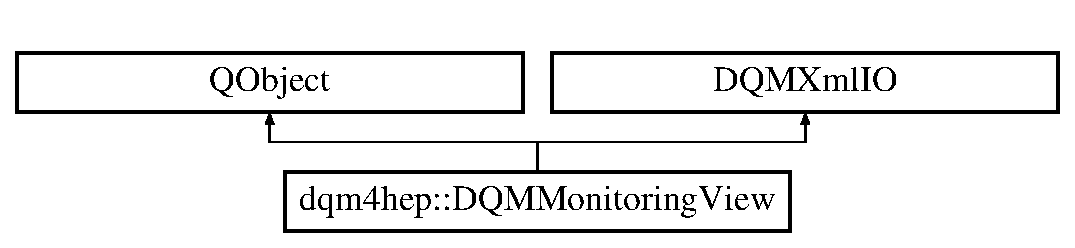
\includegraphics[height=2.000000cm]{classdqm4hep_1_1DQMMonitoringView}
\end{center}
\end{figure}
\subsection*{Public Member Functions}
\begin{DoxyCompactItemize}
\item 
{\bf D\+Q\+M\+Monitoring\+View} ({\bf D\+Q\+M\+Monitoring} $\ast$p\+Monitoring)
\begin{DoxyCompactList}\small\item\em Constructor. \end{DoxyCompactList}\item 
{\bf $\sim$\+D\+Q\+M\+Monitoring\+View} ()
\begin{DoxyCompactList}\small\item\em Destructor. \end{DoxyCompactList}\item 
{\bf D\+Q\+M\+Monitoring} $\ast$ {\bf get\+Monitoring} () const 
\begin{DoxyCompactList}\small\item\em Get the monitoring instance. \end{DoxyCompactList}\item 
Ti\+Xml\+Element $\ast$ {\bf to\+Xml} () const 
\begin{DoxyCompactList}\small\item\em Export settings to xml element. \end{DoxyCompactList}\item 
void {\bf from\+Xml} (Ti\+Xml\+Element $\ast$const p\+Xml\+Element)
\begin{DoxyCompactList}\small\item\em Import settings from xml element. \end{DoxyCompactList}\item 
void {\bf build\+View} ()
\begin{DoxyCompactList}\small\item\em Build the view. \end{DoxyCompactList}\item 
void {\bf show\+View} ()
\item 
void {\bf hide\+View} ()
\item 
{\bf D\+Q\+M\+Canvas\+View} $\ast$ {\bf get\+Canvas\+View} () const 
\item 
{\bf D\+Q\+M\+Monitor\+Element\+View} $\ast$ {\bf get\+Monitor\+Element\+View} () const 
\item 
Q\+Main\+Window $\ast$ {\bf get\+Main\+Window} () const 
\item 
void {\bf clear} ()
\end{DoxyCompactItemize}
\subsection*{Protected Member Functions}
\begin{DoxyCompactItemize}
\item 
void {\bf build\+Menus} ()
\item 
void {\bf build\+Central\+View} ()
\item 
void {\bf build\+Status\+Bar} ()
\end{DoxyCompactItemize}
\subsection*{Protected Attributes}
\begin{DoxyCompactItemize}
\item 
bool {\bf m\+\_\+view\+Built}
\begin{DoxyCompactList}\small\item\em Whether the view has been built. \end{DoxyCompactList}\item 
{\bf D\+Q\+M\+Monitoring} $\ast$ {\bf m\+\_\+p\+Monitoring}
\begin{DoxyCompactList}\small\item\em The monitoring instance. \end{DoxyCompactList}\item 
{\bf D\+Q\+M\+Canvas\+View} $\ast$ {\bf m\+\_\+p\+Canvas\+View}
\begin{DoxyCompactList}\small\item\em The canvas view to display monitor elements. \end{DoxyCompactList}\item 
{\bf D\+Q\+M\+Monitor\+Element\+View} $\ast$ {\bf m\+\_\+p\+Monitor\+Element\+View}
\begin{DoxyCompactList}\small\item\em The monitor element view to display the element hierarchy. \end{DoxyCompactList}\item 
Q\+Main\+Window $\ast$ {\bf m\+\_\+p\+Main\+Window}
\begin{DoxyCompactList}\small\item\em The main window containing the whole view. \end{DoxyCompactList}\end{DoxyCompactItemize}
\subsection*{Private Slots}
\begin{DoxyCompactItemize}
\item 
void {\bf handle\+Auto\+Update\+Button\+Clicked} ()
\end{DoxyCompactItemize}


\subsection{Detailed Description}
\doxyref{D\+Q\+M\+Monitoring\+View}{p.}{classdqm4hep_1_1DQMMonitoringView} class. 

Definition at line 49 of file D\+Q\+M\+Monitoring\+View.\+h.



\subsection{Constructor \& Destructor Documentation}
\index{dqm4hep\+::\+D\+Q\+M\+Monitoring\+View@{dqm4hep\+::\+D\+Q\+M\+Monitoring\+View}!D\+Q\+M\+Monitoring\+View@{D\+Q\+M\+Monitoring\+View}}
\index{D\+Q\+M\+Monitoring\+View@{D\+Q\+M\+Monitoring\+View}!dqm4hep\+::\+D\+Q\+M\+Monitoring\+View@{dqm4hep\+::\+D\+Q\+M\+Monitoring\+View}}
\subsubsection[{D\+Q\+M\+Monitoring\+View}]{\setlength{\rightskip}{0pt plus 5cm}dqm4hep\+::\+D\+Q\+M\+Monitoring\+View\+::\+D\+Q\+M\+Monitoring\+View (
\begin{DoxyParamCaption}
\item[{{\bf D\+Q\+M\+Monitoring} $\ast$}]{p\+Monitoring}
\end{DoxyParamCaption}
)}\label{classdqm4hep_1_1DQMMonitoringView_a6dff53f4813116562e6ed00a15eb9e76}


Constructor. 



Definition at line 83 of file D\+Q\+M\+Monitoring\+View.\+cc.



References m\+\_\+p\+Monitoring, and dqm4hep\+::\+D\+Q\+M\+Monitoring\+::set\+View().


\begin{DoxyCode}
83                                                                :
84   m_pMonitoring(pMonitoring),
85   m_pCanvasView(NULL),
86   m_pMonitorElementView(NULL),
87   m_pMainWindow(NULL),
88   m_viewBuilt(\textcolor{keyword}{false})
89 \{
90   m_pMonitoring->setView(\textcolor{keyword}{this});
91 \}
\end{DoxyCode}
\index{dqm4hep\+::\+D\+Q\+M\+Monitoring\+View@{dqm4hep\+::\+D\+Q\+M\+Monitoring\+View}!````~D\+Q\+M\+Monitoring\+View@{$\sim$\+D\+Q\+M\+Monitoring\+View}}
\index{````~D\+Q\+M\+Monitoring\+View@{$\sim$\+D\+Q\+M\+Monitoring\+View}!dqm4hep\+::\+D\+Q\+M\+Monitoring\+View@{dqm4hep\+::\+D\+Q\+M\+Monitoring\+View}}
\subsubsection[{$\sim$\+D\+Q\+M\+Monitoring\+View}]{\setlength{\rightskip}{0pt plus 5cm}dqm4hep\+::\+D\+Q\+M\+Monitoring\+View\+::$\sim$\+D\+Q\+M\+Monitoring\+View (
\begin{DoxyParamCaption}
{}
\end{DoxyParamCaption}
)}\label{classdqm4hep_1_1DQMMonitoringView_af7ab6a7a2117d806f222806ed4b87688}


Destructor. 



Definition at line 95 of file D\+Q\+M\+Monitoring\+View.\+cc.



References m\+\_\+p\+Canvas\+View, m\+\_\+p\+Main\+Window, and m\+\_\+p\+Monitor\+Element\+View.


\begin{DoxyCode}
96 \{
97   \textcolor{keywordflow}{if}(m_pCanvasView)
98     \textcolor{keyword}{delete} m_pCanvasView;
99 
100   \textcolor{keywordflow}{if}(m_pMonitorElementView)
101     \textcolor{keyword}{delete} m_pMonitorElementView;
102 
103   \textcolor{keywordflow}{if}(m_pMainWindow)
104     \textcolor{keyword}{delete} m_pMainWindow;
105 \}
\end{DoxyCode}


\subsection{Member Function Documentation}
\index{dqm4hep\+::\+D\+Q\+M\+Monitoring\+View@{dqm4hep\+::\+D\+Q\+M\+Monitoring\+View}!build\+Central\+View@{build\+Central\+View}}
\index{build\+Central\+View@{build\+Central\+View}!dqm4hep\+::\+D\+Q\+M\+Monitoring\+View@{dqm4hep\+::\+D\+Q\+M\+Monitoring\+View}}
\subsubsection[{build\+Central\+View}]{\setlength{\rightskip}{0pt plus 5cm}void dqm4hep\+::\+D\+Q\+M\+Monitoring\+View\+::build\+Central\+View (
\begin{DoxyParamCaption}
{}
\end{DoxyParamCaption}
)\hspace{0.3cm}{\ttfamily [protected]}}\label{classdqm4hep_1_1DQMMonitoringView_a6f2baff183f42ad95ba825297c7f9f82}


Definition at line 224 of file D\+Q\+M\+Monitoring\+View.\+cc.



References get\+Monitoring(), handle\+Auto\+Update\+Button\+Clicked(), m\+\_\+p\+Canvas\+View, m\+\_\+p\+Main\+Window, m\+\_\+p\+Monitor\+Element\+View, and m\+\_\+p\+Monitoring.



Referenced by build\+View().


\begin{DoxyCode}
225 \{
226   \textcolor{comment}{// main area}
227   QSplitter *pMainWidget = \textcolor{keyword}{new} QSplitter(Qt::Horizontal);
228   m_pMainWindow->setCentralWidget(pMainWidget);
229 
230   QWidget *pLeftViewWidget = \textcolor{keyword}{new} QWidget();
231   pLeftViewWidget->setLayout(\textcolor{keyword}{new} QVBoxLayout());
232 
233 
234     \textcolor{comment}{// update buttons}
235   QWidget *pUpdateButtonAreaWidget = \textcolor{keyword}{new} QWidget();
236   pUpdateButtonAreaWidget->setLayout(\textcolor{keyword}{new} QHBoxLayout());
237 
238   QPushButton *pAutoUpdateButton = \textcolor{keyword}{new} QPushButton(\textcolor{stringliteral}{"Start update"});
239   pUpdateButtonAreaWidget->layout()->addWidget(pAutoUpdateButton);
240 
241   QPushButton *pUpdateButton = \textcolor{keyword}{new} QPushButton(\textcolor{stringliteral}{"Update"});
242   pUpdateButtonAreaWidget->layout()->addWidget(pUpdateButton);
243 
244   pUpdateButtonAreaWidget->setMaximumHeight(50);
245   pLeftViewWidget->layout()->addWidget(pUpdateButtonAreaWidget);
246 
247 
248   \textcolor{comment}{// monitor element contents view}
249   QGroupBox *pContentGroupBox = \textcolor{keyword}{new} QGroupBox(\textcolor{stringliteral}{"Contents"});
250   pContentGroupBox->setLayout(\textcolor{keyword}{new} QVBoxLayout());
251   pLeftViewWidget->layout()->addWidget(pContentGroupBox);
252 
253   m_pMonitorElementView = \textcolor{keyword}{new} DQMMonitorElementView(m_pMonitoring);
254   m_pMonitorElementView->setSizePolicy(QSizePolicy::Expanding, QSizePolicy::Expanding);
255   pContentGroupBox->layout()->addWidget(m_pMonitorElementView);
256 
257 
258   \textcolor{comment}{// clear and browse buttons}
259   QWidget *pClearBrowseButtonAreaWidget = \textcolor{keyword}{new} QWidget();
260   pClearBrowseButtonAreaWidget->setLayout(\textcolor{keyword}{new} QHBoxLayout());
261 
262   QPushButton *pClearButton = \textcolor{keyword}{new} QPushButton(\textcolor{stringliteral}{"Clear"});
263   pClearBrowseButtonAreaWidget->layout()->addWidget(pClearButton);
264 
265   QPushButton *pBrowseButton = \textcolor{keyword}{new} QPushButton(\textcolor{stringliteral}{"Browse"});
266   pClearBrowseButtonAreaWidget->layout()->addWidget(pBrowseButton);
267 
268   pClearBrowseButtonAreaWidget->setMaximumHeight(50);
269     pLeftViewWidget->layout()->addWidget(pClearBrowseButtonAreaWidget);
270 
271 
272   pMainWidget->addWidget(pLeftViewWidget);
273 
274   m_pCanvasView = \textcolor{keyword}{new} DQMCanvasView(m_pMonitoring);
275   pMainWidget->addWidget(m_pCanvasView);
276 
277   connect(pAutoUpdateButton, SIGNAL(clicked()), \textcolor{keyword}{this}, SLOT(
      handleAutoUpdateButtonClicked()));
278   connect(pUpdateButton, SIGNAL(clicked()), this->getMonitoring()->getController(), SLOT(
      querySubscribedMonitorElements()));
279   connect(pClearButton, SIGNAL(clicked()), this->getMonitoring()->getController(), SLOT(clearMonitoring()))
      ;
280   connect(pBrowseButton, SIGNAL(clicked()), this->getMonitoring()->getController(), SLOT(openBrowser()));
281 \}
\end{DoxyCode}
\index{dqm4hep\+::\+D\+Q\+M\+Monitoring\+View@{dqm4hep\+::\+D\+Q\+M\+Monitoring\+View}!build\+Menus@{build\+Menus}}
\index{build\+Menus@{build\+Menus}!dqm4hep\+::\+D\+Q\+M\+Monitoring\+View@{dqm4hep\+::\+D\+Q\+M\+Monitoring\+View}}
\subsubsection[{build\+Menus}]{\setlength{\rightskip}{0pt plus 5cm}void dqm4hep\+::\+D\+Q\+M\+Monitoring\+View\+::build\+Menus (
\begin{DoxyParamCaption}
{}
\end{DoxyParamCaption}
)\hspace{0.3cm}{\ttfamily [protected]}}\label{classdqm4hep_1_1DQMMonitoringView_ad6646de01e5b083710b7fb79c88ed09b}


Definition at line 199 of file D\+Q\+M\+Monitoring\+View.\+cc.



References get\+Monitoring(), and m\+\_\+p\+Main\+Window.



Referenced by build\+View().


\begin{DoxyCode}
200 \{
201   QMenu *pFileMenu = m_pMainWindow->menuBar()->addMenu(\textcolor{stringliteral}{"&File"});
202 
203   pFileMenu->addAction(\textcolor{stringliteral}{"&Import"}, this->getMonitoring()->getController(), SLOT(openFile()), QKeySequence(
      QKeySequence::Open));
204   pFileMenu->addAction(\textcolor{stringliteral}{"&Export"}, this->getMonitoring()->getController(), SLOT(saveAs()), QKeySequence(
      QKeySequence::SaveAs));
205   pFileMenu->addSeparator();
206   pFileMenu->addAction(\textcolor{stringliteral}{"&Browse"}, this->getMonitoring()->getController(), SLOT(openBrowser()), QKeySequence
      (QKeySequence::New));
207   pFileMenu->addSeparator();
208   pFileMenu->addAction(\textcolor{stringliteral}{"&Quit"}, this->getMonitoring()->getController(), SLOT(quit()), QKeySequence(
      QKeySequence::Quit));
209 
210   QMenu *pHelpMenu = m_pMainWindow->menuBar()->addMenu(\textcolor{stringliteral}{"&Help"});
211 
212   pHelpMenu->addAction(\textcolor{stringliteral}{"Doxygen"}, this->getMonitoring()->getController(), SLOT(openDoxygenDoc()));
213   pHelpMenu->addAction(\textcolor{stringliteral}{"User guide"}, this->getMonitoring()->getController(), SLOT(openUserGuide()));
214   pHelpMenu->addSeparator();
215   pHelpMenu->addAction(\textcolor{stringliteral}{"Contribute"}, this->getMonitoring()->getController(), SLOT(openGithubPage()));
216   pHelpMenu->addAction(\textcolor{stringliteral}{"Report bugs"}, this->getMonitoring()->getController(), SLOT(openIssuesPage()));
217   pHelpMenu->addSeparator();
218   pHelpMenu->addAction(\textcolor{stringliteral}{"About Qt"}, qApp, SLOT(aboutQt()));
219   pHelpMenu->addAction(\textcolor{stringliteral}{"About DQM4HEP"}, this->getMonitoring()->getController(), SLOT(aboutDQM4HEP()));
220 \}
\end{DoxyCode}
\index{dqm4hep\+::\+D\+Q\+M\+Monitoring\+View@{dqm4hep\+::\+D\+Q\+M\+Monitoring\+View}!build\+Status\+Bar@{build\+Status\+Bar}}
\index{build\+Status\+Bar@{build\+Status\+Bar}!dqm4hep\+::\+D\+Q\+M\+Monitoring\+View@{dqm4hep\+::\+D\+Q\+M\+Monitoring\+View}}
\subsubsection[{build\+Status\+Bar}]{\setlength{\rightskip}{0pt plus 5cm}void dqm4hep\+::\+D\+Q\+M\+Monitoring\+View\+::build\+Status\+Bar (
\begin{DoxyParamCaption}
{}
\end{DoxyParamCaption}
)\hspace{0.3cm}{\ttfamily [protected]}}\label{classdqm4hep_1_1DQMMonitoringView_acb713ae3c62a065532d6b2e5afb215a9}


Definition at line 285 of file D\+Q\+M\+Monitoring\+View.\+cc.



References get\+Main\+Window().



Referenced by build\+View().


\begin{DoxyCode}
286 \{
287   this->getMainWindow()->statusBar()->showMessage(\textcolor{stringliteral}{"Welcome"}, 3000);
288 \}
\end{DoxyCode}
\index{dqm4hep\+::\+D\+Q\+M\+Monitoring\+View@{dqm4hep\+::\+D\+Q\+M\+Monitoring\+View}!build\+View@{build\+View}}
\index{build\+View@{build\+View}!dqm4hep\+::\+D\+Q\+M\+Monitoring\+View@{dqm4hep\+::\+D\+Q\+M\+Monitoring\+View}}
\subsubsection[{build\+View}]{\setlength{\rightskip}{0pt plus 5cm}void dqm4hep\+::\+D\+Q\+M\+Monitoring\+View\+::build\+View (
\begin{DoxyParamCaption}
{}
\end{DoxyParamCaption}
)}\label{classdqm4hep_1_1DQMMonitoringView_a589aaf092037007198d76ca5272bb231}


Build the view. 

Should be called once 

Definition at line 178 of file D\+Q\+M\+Monitoring\+View.\+cc.



References build\+Central\+View(), build\+Menus(), build\+Status\+Bar(), D\+Q\+M\+Viz\+\_\+\+D\+I\+R, get\+Monitoring(), m\+\_\+p\+Main\+Window, and m\+\_\+view\+Built.



Referenced by hide\+View(), and show\+View().


\begin{DoxyCode}
179 \{
180   \textcolor{keywordflow}{if}(m_viewBuilt)
181     \textcolor{keywordflow}{return};
182 
183   m_pMainWindow = \textcolor{keyword}{new} DQMMonitoringMainWindow(this->getMonitoring());
184   m_pMainWindow->setWindowTitle(\textcolor{stringliteral}{"DQM Monitoring"});
185   m_pMainWindow->setAnimated(\textcolor{keyword}{true});
186 
187   QString iconDir = QString(DQMViz_DIR) + \textcolor{stringliteral}{"/icons"};
188   m_pMainWindow->setWindowIcon(QIcon(iconDir + \textcolor{stringliteral}{"/MON\_WIN.png"}));
189 
190   buildMenus();
191   buildCentralView();
192   buildStatusBar();
193 
194   m_viewBuilt = \textcolor{keyword}{true};
195 \}
\end{DoxyCode}
\index{dqm4hep\+::\+D\+Q\+M\+Monitoring\+View@{dqm4hep\+::\+D\+Q\+M\+Monitoring\+View}!clear@{clear}}
\index{clear@{clear}!dqm4hep\+::\+D\+Q\+M\+Monitoring\+View@{dqm4hep\+::\+D\+Q\+M\+Monitoring\+View}}
\subsubsection[{clear}]{\setlength{\rightskip}{0pt plus 5cm}void dqm4hep\+::\+D\+Q\+M\+Monitoring\+View\+::clear (
\begin{DoxyParamCaption}
{}
\end{DoxyParamCaption}
)}\label{classdqm4hep_1_1DQMMonitoringView_a69698bb027c68296194ee01ae4d4c623}


Definition at line 308 of file D\+Q\+M\+Monitoring\+View.\+cc.



References dqm4hep\+::\+D\+Q\+M\+Canvas\+View\+::clear(), dqm4hep\+::\+D\+Q\+M\+Monitor\+Element\+View\+::clear(), m\+\_\+p\+Canvas\+View, and m\+\_\+p\+Monitor\+Element\+View.



Referenced by dqm4hep\+::\+D\+Q\+M\+Monitoring\+Controller\+::clear\+Monitoring(), dqm4hep\+::\+D\+Q\+M\+Monitoring\+Controller\+::clear\+View\+And\+Model(), from\+Xml(), and dqm4hep\+::\+D\+Q\+M\+Monitoring\+Controller\+::open\+File().


\begin{DoxyCode}
309 \{
310   m_pMonitorElementView->clear();
311   m_pCanvasView->clear();
312 \}
\end{DoxyCode}
\index{dqm4hep\+::\+D\+Q\+M\+Monitoring\+View@{dqm4hep\+::\+D\+Q\+M\+Monitoring\+View}!from\+Xml@{from\+Xml}}
\index{from\+Xml@{from\+Xml}!dqm4hep\+::\+D\+Q\+M\+Monitoring\+View@{dqm4hep\+::\+D\+Q\+M\+Monitoring\+View}}
\subsubsection[{from\+Xml}]{\setlength{\rightskip}{0pt plus 5cm}void dqm4hep\+::\+D\+Q\+M\+Monitoring\+View\+::from\+Xml (
\begin{DoxyParamCaption}
\item[{Ti\+Xml\+Element $\ast$const}]{p\+Xml\+Element}
\end{DoxyParamCaption}
)}\label{classdqm4hep_1_1DQMMonitoringView_ab0d663182499725c43e778cae5fd44ea}


Import settings from xml element. 



Definition at line 135 of file D\+Q\+M\+Monitoring\+View.\+cc.



References clear(), dqm4hep\+::\+D\+Q\+M\+Canvas\+View\+::from\+Xml(), dqm4hep\+::\+D\+Q\+M\+Monitor\+Element\+View\+::from\+Xml(), m\+\_\+p\+Canvas\+View, and m\+\_\+p\+Monitor\+Element\+View.



Referenced by dqm4hep\+::\+D\+Q\+M\+Monitoring\+Controller\+::open\+File().


\begin{DoxyCode}
136 \{
137   \textcolor{keywordflow}{if}(!pXmlElement)
138     \textcolor{keywordflow}{return};
139 
140   this->clear();
141 
142     TiXmlHandle elementHandle(pXmlElement);
143 
144     TiXmlElement *pCanvasViewElement = elementHandle.FirstChild(\textcolor{stringliteral}{"canvasView"}).Element();
145 
146     \textcolor{keywordflow}{if}(pCanvasViewElement)
147       m_pCanvasView->fromXml(pCanvasViewElement);
148 
149     TiXmlElement *pMeViewElement = elementHandle.FirstChild(\textcolor{stringliteral}{"meView"}).Element();
150 
151     \textcolor{keywordflow}{if}(pMeViewElement)
152       m_pMonitorElementView->fromXml(pMeViewElement);
153 \}
\end{DoxyCode}
\index{dqm4hep\+::\+D\+Q\+M\+Monitoring\+View@{dqm4hep\+::\+D\+Q\+M\+Monitoring\+View}!get\+Canvas\+View@{get\+Canvas\+View}}
\index{get\+Canvas\+View@{get\+Canvas\+View}!dqm4hep\+::\+D\+Q\+M\+Monitoring\+View@{dqm4hep\+::\+D\+Q\+M\+Monitoring\+View}}
\subsubsection[{get\+Canvas\+View}]{\setlength{\rightskip}{0pt plus 5cm}{\bf D\+Q\+M\+Canvas\+View} $\ast$ dqm4hep\+::\+D\+Q\+M\+Monitoring\+View\+::get\+Canvas\+View (
\begin{DoxyParamCaption}
{}
\end{DoxyParamCaption}
) const}\label{classdqm4hep_1_1DQMMonitoringView_afd18c51df68d552b90e9d49050c69cc2}


Definition at line 157 of file D\+Q\+M\+Monitoring\+View.\+cc.



References m\+\_\+p\+Canvas\+View.



Referenced by dqm4hep\+::\+D\+Q\+M\+Root\+Widget\+::create\+Context\+Menu(), dqm4hep\+::\+D\+Q\+M\+Monitor\+Element\+Navigator\+::draw\+Selected\+Monitor\+Elements(), dqm4hep\+::\+D\+Q\+M\+Monitor\+Element\+Navigator\+::handle\+Item\+Double\+Click(), dqm4hep\+::\+D\+Q\+M\+Monitor\+Element\+Navigator\+::key\+Press\+Event(), dqm4hep\+::\+D\+Q\+M\+Root\+Widget\+::move\+Canvas(), dqm4hep\+::\+D\+Q\+M\+Root\+Widget\+::remove\+Canvas(), and dqm4hep\+::\+D\+Q\+M\+Monitor\+Element\+Navigator\+::show\+Context\+Menu().


\begin{DoxyCode}
158 \{
159   \textcolor{keywordflow}{return} m_pCanvasView;
160 \}
\end{DoxyCode}
\index{dqm4hep\+::\+D\+Q\+M\+Monitoring\+View@{dqm4hep\+::\+D\+Q\+M\+Monitoring\+View}!get\+Main\+Window@{get\+Main\+Window}}
\index{get\+Main\+Window@{get\+Main\+Window}!dqm4hep\+::\+D\+Q\+M\+Monitoring\+View@{dqm4hep\+::\+D\+Q\+M\+Monitoring\+View}}
\subsubsection[{get\+Main\+Window}]{\setlength{\rightskip}{0pt plus 5cm}Q\+Main\+Window $\ast$ dqm4hep\+::\+D\+Q\+M\+Monitoring\+View\+::get\+Main\+Window (
\begin{DoxyParamCaption}
{}
\end{DoxyParamCaption}
) const}\label{classdqm4hep_1_1DQMMonitoringView_a3552a6afba033465b3a282ff8acaf25d}


Definition at line 171 of file D\+Q\+M\+Monitoring\+View.\+cc.



References m\+\_\+p\+Main\+Window.



Referenced by build\+Status\+Bar(), hide\+View(), dqm4hep\+::\+D\+Q\+M\+Monitoring\+Controller\+::log(), and show\+View().


\begin{DoxyCode}
172 \{
173   \textcolor{keywordflow}{return} m_pMainWindow;
174 \}
\end{DoxyCode}
\index{dqm4hep\+::\+D\+Q\+M\+Monitoring\+View@{dqm4hep\+::\+D\+Q\+M\+Monitoring\+View}!get\+Monitor\+Element\+View@{get\+Monitor\+Element\+View}}
\index{get\+Monitor\+Element\+View@{get\+Monitor\+Element\+View}!dqm4hep\+::\+D\+Q\+M\+Monitoring\+View@{dqm4hep\+::\+D\+Q\+M\+Monitoring\+View}}
\subsubsection[{get\+Monitor\+Element\+View}]{\setlength{\rightskip}{0pt plus 5cm}{\bf D\+Q\+M\+Monitor\+Element\+View} $\ast$ dqm4hep\+::\+D\+Q\+M\+Monitoring\+View\+::get\+Monitor\+Element\+View (
\begin{DoxyParamCaption}
{}
\end{DoxyParamCaption}
) const}\label{classdqm4hep_1_1DQMMonitoringView_a47d2e6cc2aa12782cf0b0d102ffc7f70}


Definition at line 164 of file D\+Q\+M\+Monitoring\+View.\+cc.



References m\+\_\+p\+Monitor\+Element\+View.



Referenced by dqm4hep\+::\+D\+Q\+M\+Monitoring\+Model\+::clear(), dqm4hep\+::\+D\+Q\+M\+Monitoring\+Model\+::get\+Or\+Create\+Gui\+Monitor\+Element(), dqm4hep\+::\+D\+Q\+M\+Monitoring\+Controller\+::handle\+Server\+Shutdown(), dqm4hep\+::\+D\+Q\+M\+Monitoring\+Controller\+::handle\+Server\+Startup(), dqm4hep\+::\+D\+Q\+M\+Monitoring\+Model\+::load\+Monitor\+Element\+Info\+List(), dqm4hep\+::\+D\+Q\+M\+Monitoring\+Model\+::remove\+Monitor\+Element(), and dqm4hep\+::\+D\+Q\+M\+Monitoring\+Model\+::update\+Monitor\+Element().


\begin{DoxyCode}
165 \{
166   \textcolor{keywordflow}{return} m_pMonitorElementView;
167 \}
\end{DoxyCode}
\index{dqm4hep\+::\+D\+Q\+M\+Monitoring\+View@{dqm4hep\+::\+D\+Q\+M\+Monitoring\+View}!get\+Monitoring@{get\+Monitoring}}
\index{get\+Monitoring@{get\+Monitoring}!dqm4hep\+::\+D\+Q\+M\+Monitoring\+View@{dqm4hep\+::\+D\+Q\+M\+Monitoring\+View}}
\subsubsection[{get\+Monitoring}]{\setlength{\rightskip}{0pt plus 5cm}{\bf D\+Q\+M\+Monitoring} $\ast$ dqm4hep\+::\+D\+Q\+M\+Monitoring\+View\+::get\+Monitoring (
\begin{DoxyParamCaption}
{}
\end{DoxyParamCaption}
) const}\label{classdqm4hep_1_1DQMMonitoringView_ad205862fac4c4a070b61c8fb4b67b569}


Get the monitoring instance. 



Definition at line 109 of file D\+Q\+M\+Monitoring\+View.\+cc.



References m\+\_\+p\+Monitoring.



Referenced by build\+Central\+View(), build\+Menus(), build\+View(), and handle\+Auto\+Update\+Button\+Clicked().


\begin{DoxyCode}
110 \{
111   \textcolor{keywordflow}{return} m_pMonitoring;
112 \}
\end{DoxyCode}
\index{dqm4hep\+::\+D\+Q\+M\+Monitoring\+View@{dqm4hep\+::\+D\+Q\+M\+Monitoring\+View}!handle\+Auto\+Update\+Button\+Clicked@{handle\+Auto\+Update\+Button\+Clicked}}
\index{handle\+Auto\+Update\+Button\+Clicked@{handle\+Auto\+Update\+Button\+Clicked}!dqm4hep\+::\+D\+Q\+M\+Monitoring\+View@{dqm4hep\+::\+D\+Q\+M\+Monitoring\+View}}
\subsubsection[{handle\+Auto\+Update\+Button\+Clicked}]{\setlength{\rightskip}{0pt plus 5cm}void dqm4hep\+::\+D\+Q\+M\+Monitoring\+View\+::handle\+Auto\+Update\+Button\+Clicked (
\begin{DoxyParamCaption}
{}
\end{DoxyParamCaption}
)\hspace{0.3cm}{\ttfamily [private]}, {\ttfamily [slot]}}\label{classdqm4hep_1_1DQMMonitoringView_a4f55aab1b801e16c324f067c5f09d42d}


Definition at line 316 of file D\+Q\+M\+Monitoring\+View.\+cc.



References dqm4hep\+::\+D\+Q\+M\+Monitoring\+::get\+Controller(), get\+Monitoring(), dqm4hep\+::\+D\+Q\+M\+Monitoring\+Controller\+::get\+Update\+Mode(), and dqm4hep\+::\+D\+Q\+M\+Monitoring\+Controller\+::set\+Update\+Mode().



Referenced by build\+Central\+View().


\begin{DoxyCode}
317 \{
318   QPushButton *pButton = qobject\_cast<QPushButton *>(sender());
319 
320   \textcolor{keywordflow}{if}(!pButton)
321     \textcolor{keywordflow}{return};
322 
323   \textcolor{comment}{// update view}
324   \textcolor{keywordflow}{if}(this->getMonitoring()->getController()->getUpdateMode())
325   \{
326     pButton->setText(\textcolor{stringliteral}{"Start update"});
327     this->getMonitoring()->getController()->setUpdateMode(\textcolor{keyword}{false});
328   \}
329   \textcolor{keywordflow}{else}
330   \{
331     pButton->setText(\textcolor{stringliteral}{"Stop update"});
332     this->getMonitoring()->getController()->setUpdateMode(\textcolor{keyword}{true});
333   \}
334 \}
\end{DoxyCode}
\index{dqm4hep\+::\+D\+Q\+M\+Monitoring\+View@{dqm4hep\+::\+D\+Q\+M\+Monitoring\+View}!hide\+View@{hide\+View}}
\index{hide\+View@{hide\+View}!dqm4hep\+::\+D\+Q\+M\+Monitoring\+View@{dqm4hep\+::\+D\+Q\+M\+Monitoring\+View}}
\subsubsection[{hide\+View}]{\setlength{\rightskip}{0pt plus 5cm}void dqm4hep\+::\+D\+Q\+M\+Monitoring\+View\+::hide\+View (
\begin{DoxyParamCaption}
{}
\end{DoxyParamCaption}
)}\label{classdqm4hep_1_1DQMMonitoringView_ade2429a518ceddc1c41e03b3342c3ef7}


Definition at line 300 of file D\+Q\+M\+Monitoring\+View.\+cc.



References build\+View(), and get\+Main\+Window().


\begin{DoxyCode}
301 \{
302   this->buildView();
303   this->getMainWindow()->showMinimized();
304 \}
\end{DoxyCode}
\index{dqm4hep\+::\+D\+Q\+M\+Monitoring\+View@{dqm4hep\+::\+D\+Q\+M\+Monitoring\+View}!show\+View@{show\+View}}
\index{show\+View@{show\+View}!dqm4hep\+::\+D\+Q\+M\+Monitoring\+View@{dqm4hep\+::\+D\+Q\+M\+Monitoring\+View}}
\subsubsection[{show\+View}]{\setlength{\rightskip}{0pt plus 5cm}void dqm4hep\+::\+D\+Q\+M\+Monitoring\+View\+::show\+View (
\begin{DoxyParamCaption}
{}
\end{DoxyParamCaption}
)}\label{classdqm4hep_1_1DQMMonitoringView_a84df8b712232ada23337dbe131374445}


Definition at line 292 of file D\+Q\+M\+Monitoring\+View.\+cc.



References build\+View(), and get\+Main\+Window().


\begin{DoxyCode}
293 \{
294   this->buildView();
295   this->getMainWindow()->show();
296 \}
\end{DoxyCode}
\index{dqm4hep\+::\+D\+Q\+M\+Monitoring\+View@{dqm4hep\+::\+D\+Q\+M\+Monitoring\+View}!to\+Xml@{to\+Xml}}
\index{to\+Xml@{to\+Xml}!dqm4hep\+::\+D\+Q\+M\+Monitoring\+View@{dqm4hep\+::\+D\+Q\+M\+Monitoring\+View}}
\subsubsection[{to\+Xml}]{\setlength{\rightskip}{0pt plus 5cm}Ti\+Xml\+Element $\ast$ dqm4hep\+::\+D\+Q\+M\+Monitoring\+View\+::to\+Xml (
\begin{DoxyParamCaption}
{}
\end{DoxyParamCaption}
) const}\label{classdqm4hep_1_1DQMMonitoringView_ab2b686c6f76afc5008341b8c8524a107}


Export settings to xml element. 



Definition at line 116 of file D\+Q\+M\+Monitoring\+View.\+cc.



References m\+\_\+p\+Canvas\+View, m\+\_\+p\+Monitor\+Element\+View, dqm4hep\+::\+D\+Q\+M\+Canvas\+View\+::to\+Xml(), and dqm4hep\+::\+D\+Q\+M\+Monitor\+Element\+View\+::to\+Xml().



Referenced by dqm4hep\+::\+D\+Q\+M\+Monitoring\+Controller\+::save\+As().


\begin{DoxyCode}
117 \{
118   TiXmlElement *pXmlElement = \textcolor{keyword}{new} TiXmlElement(\textcolor{stringliteral}{"view"});
119 
120   TiXmlElement *pMeViewElement = m_pMonitorElementView->toXml();
121 
122   \textcolor{keywordflow}{if}(pMeViewElement)
123     pXmlElement->LinkEndChild(pMeViewElement);
124 
125   TiXmlElement *pCanvasViewElement = m_pCanvasView->toXml();
126 
127   \textcolor{keywordflow}{if}(pCanvasViewElement)
128     pXmlElement->LinkEndChild(pCanvasViewElement);
129 
130   \textcolor{keywordflow}{return} pXmlElement;
131 \}
\end{DoxyCode}


\subsection{Member Data Documentation}
\index{dqm4hep\+::\+D\+Q\+M\+Monitoring\+View@{dqm4hep\+::\+D\+Q\+M\+Monitoring\+View}!m\+\_\+p\+Canvas\+View@{m\+\_\+p\+Canvas\+View}}
\index{m\+\_\+p\+Canvas\+View@{m\+\_\+p\+Canvas\+View}!dqm4hep\+::\+D\+Q\+M\+Monitoring\+View@{dqm4hep\+::\+D\+Q\+M\+Monitoring\+View}}
\subsubsection[{m\+\_\+p\+Canvas\+View}]{\setlength{\rightskip}{0pt plus 5cm}{\bf D\+Q\+M\+Canvas\+View}$\ast$ dqm4hep\+::\+D\+Q\+M\+Monitoring\+View\+::m\+\_\+p\+Canvas\+View\hspace{0.3cm}{\ttfamily [protected]}}\label{classdqm4hep_1_1DQMMonitoringView_a9a591427f14d0714c54be9675d04b25a}


The canvas view to display monitor elements. 



Definition at line 126 of file D\+Q\+M\+Monitoring\+View.\+h.



Referenced by build\+Central\+View(), clear(), from\+Xml(), get\+Canvas\+View(), to\+Xml(), and $\sim$\+D\+Q\+M\+Monitoring\+View().

\index{dqm4hep\+::\+D\+Q\+M\+Monitoring\+View@{dqm4hep\+::\+D\+Q\+M\+Monitoring\+View}!m\+\_\+p\+Main\+Window@{m\+\_\+p\+Main\+Window}}
\index{m\+\_\+p\+Main\+Window@{m\+\_\+p\+Main\+Window}!dqm4hep\+::\+D\+Q\+M\+Monitoring\+View@{dqm4hep\+::\+D\+Q\+M\+Monitoring\+View}}
\subsubsection[{m\+\_\+p\+Main\+Window}]{\setlength{\rightskip}{0pt plus 5cm}Q\+Main\+Window$\ast$ dqm4hep\+::\+D\+Q\+M\+Monitoring\+View\+::m\+\_\+p\+Main\+Window\hspace{0.3cm}{\ttfamily [protected]}}\label{classdqm4hep_1_1DQMMonitoringView_aa5466076940afe71d74c889cab6403ca}


The main window containing the whole view. 



Definition at line 128 of file D\+Q\+M\+Monitoring\+View.\+h.



Referenced by build\+Central\+View(), build\+Menus(), build\+View(), get\+Main\+Window(), and $\sim$\+D\+Q\+M\+Monitoring\+View().

\index{dqm4hep\+::\+D\+Q\+M\+Monitoring\+View@{dqm4hep\+::\+D\+Q\+M\+Monitoring\+View}!m\+\_\+p\+Monitor\+Element\+View@{m\+\_\+p\+Monitor\+Element\+View}}
\index{m\+\_\+p\+Monitor\+Element\+View@{m\+\_\+p\+Monitor\+Element\+View}!dqm4hep\+::\+D\+Q\+M\+Monitoring\+View@{dqm4hep\+::\+D\+Q\+M\+Monitoring\+View}}
\subsubsection[{m\+\_\+p\+Monitor\+Element\+View}]{\setlength{\rightskip}{0pt plus 5cm}{\bf D\+Q\+M\+Monitor\+Element\+View}$\ast$ dqm4hep\+::\+D\+Q\+M\+Monitoring\+View\+::m\+\_\+p\+Monitor\+Element\+View\hspace{0.3cm}{\ttfamily [protected]}}\label{classdqm4hep_1_1DQMMonitoringView_a52c0ecfd71d022d4d84ce0cc646c8cc5}


The monitor element view to display the element hierarchy. 



Definition at line 127 of file D\+Q\+M\+Monitoring\+View.\+h.



Referenced by build\+Central\+View(), clear(), from\+Xml(), get\+Monitor\+Element\+View(), to\+Xml(), and $\sim$\+D\+Q\+M\+Monitoring\+View().

\index{dqm4hep\+::\+D\+Q\+M\+Monitoring\+View@{dqm4hep\+::\+D\+Q\+M\+Monitoring\+View}!m\+\_\+p\+Monitoring@{m\+\_\+p\+Monitoring}}
\index{m\+\_\+p\+Monitoring@{m\+\_\+p\+Monitoring}!dqm4hep\+::\+D\+Q\+M\+Monitoring\+View@{dqm4hep\+::\+D\+Q\+M\+Monitoring\+View}}
\subsubsection[{m\+\_\+p\+Monitoring}]{\setlength{\rightskip}{0pt plus 5cm}{\bf D\+Q\+M\+Monitoring}$\ast$ dqm4hep\+::\+D\+Q\+M\+Monitoring\+View\+::m\+\_\+p\+Monitoring\hspace{0.3cm}{\ttfamily [protected]}}\label{classdqm4hep_1_1DQMMonitoringView_a0fa7a834b09f7f28eff3fe72a241dc5a}


The monitoring instance. 



Definition at line 125 of file D\+Q\+M\+Monitoring\+View.\+h.



Referenced by build\+Central\+View(), D\+Q\+M\+Monitoring\+View(), and get\+Monitoring().

\index{dqm4hep\+::\+D\+Q\+M\+Monitoring\+View@{dqm4hep\+::\+D\+Q\+M\+Monitoring\+View}!m\+\_\+view\+Built@{m\+\_\+view\+Built}}
\index{m\+\_\+view\+Built@{m\+\_\+view\+Built}!dqm4hep\+::\+D\+Q\+M\+Monitoring\+View@{dqm4hep\+::\+D\+Q\+M\+Monitoring\+View}}
\subsubsection[{m\+\_\+view\+Built}]{\setlength{\rightskip}{0pt plus 5cm}bool dqm4hep\+::\+D\+Q\+M\+Monitoring\+View\+::m\+\_\+view\+Built\hspace{0.3cm}{\ttfamily [protected]}}\label{classdqm4hep_1_1DQMMonitoringView_a7fd354df2cd5318e3e099b5076c8fedf}


Whether the view has been built. 



Definition at line 123 of file D\+Q\+M\+Monitoring\+View.\+h.



Referenced by build\+View().



The documentation for this class was generated from the following files\+:\begin{DoxyCompactItemize}
\item 
{\bf D\+Q\+M\+Monitoring\+View.\+h}\item 
{\bf D\+Q\+M\+Monitoring\+View.\+cc}\end{DoxyCompactItemize}

\section{dqm4hep\+:\+:D\+Q\+M\+Root\+Widget Class Reference}
\label{classdqm4hep_1_1DQMRootWidget}\index{dqm4hep\+::\+D\+Q\+M\+Root\+Widget@{dqm4hep\+::\+D\+Q\+M\+Root\+Widget}}


\doxyref{D\+Q\+M\+Root\+Widget}{p.}{classdqm4hep_1_1DQMRootWidget} class.  




{\ttfamily \#include $<$D\+Q\+M\+Root\+Widget.\+h$>$}

Inheritance diagram for dqm4hep\+:\+:D\+Q\+M\+Root\+Widget\+:\begin{figure}[H]
\begin{center}
\leavevmode
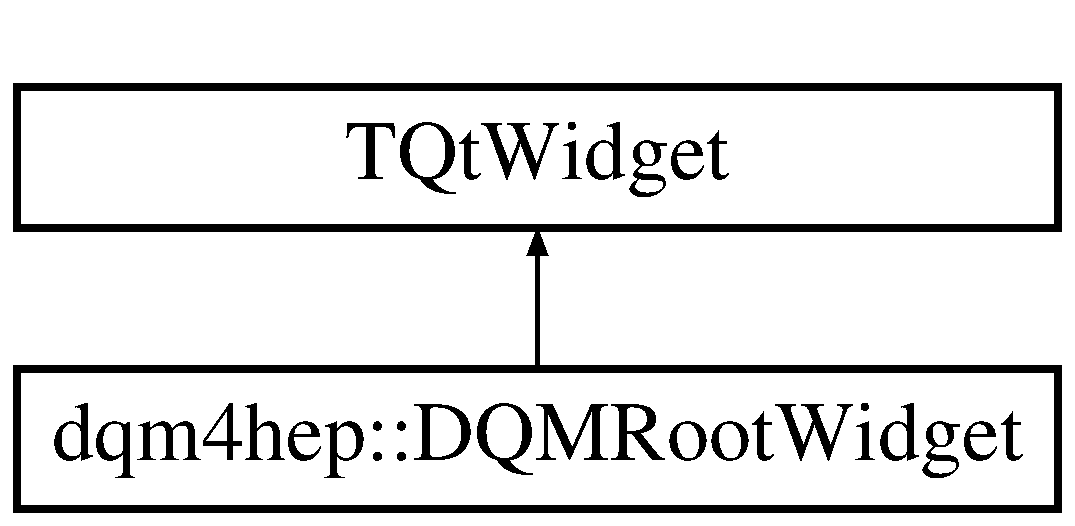
\includegraphics[height=2.000000cm]{classdqm4hep_1_1DQMRootWidget}
\end{center}
\end{figure}
\subsection*{Public Member Functions}
\begin{DoxyCompactItemize}
\item 
{\bf D\+Q\+M\+Root\+Widget} ({\bf D\+Q\+M\+Monitoring} $\ast$p\+Monitoring, Q\+Widget $\ast$p\+Parent=0)
\begin{DoxyCompactList}\small\item\em Constructor. \end{DoxyCompactList}\item 
{\bf $\sim$\+D\+Q\+M\+Root\+Widget} ()
\begin{DoxyCompactList}\small\item\em Destructor. \end{DoxyCompactList}\item 
{\bf D\+Q\+M\+Monitoring} $\ast$ {\bf get\+Monitoring} () const 
\begin{DoxyCompactList}\small\item\em Get the monitoring instance. \end{DoxyCompactList}\item 
void {\bf set\+Canvas} ({\bf D\+Q\+M\+Canvas} $\ast$p\+Canvas)
\begin{DoxyCompactList}\small\item\em Set canvas on which the the root widget is drawn. \end{DoxyCompactList}\item 
{\bf D\+Q\+M\+Canvas} $\ast$ {\bf get\+Canvas} () const 
\begin{DoxyCompactList}\small\item\em Get the canvas on which the the root widget is drawn. \end{DoxyCompactList}\item 
virtual void {\bf mouse\+Double\+Click\+Event} (Q\+Mouse\+Event $\ast$e)
\begin{DoxyCompactList}\small\item\em Handle mouse double click event on the widget. \end{DoxyCompactList}\item 
virtual void {\bf mouse\+Release\+Event} (Q\+Mouse\+Event $\ast$e)
\begin{DoxyCompactList}\small\item\em Handle mouse release event on the widget. \end{DoxyCompactList}\item 
virtual void {\bf post\+Draw} ()
\begin{DoxyCompactList}\small\item\em Post draw function with a 'fake' update of the widget. \end{DoxyCompactList}\item 
virtual void {\bf draw\+No\+Vis} ()
\begin{DoxyCompactList}\small\item\em Draw an image saying \char`\"{}no vis available\char`\"{}. \end{DoxyCompactList}\item 
virtual void {\bf draw} ({\bf D\+Q\+M\+Gui\+Monitor\+Element} $\ast$p\+Monitor\+Element)
\begin{DoxyCompactList}\small\item\em Draw the monitor element on the canvas. \end{DoxyCompactList}\item 
virtual T\+Image $\ast$ {\bf get\+No\+Vis\+Image} ()
\begin{DoxyCompactList}\small\item\em Get the \char`\"{}no vis\char`\"{} image, create it if not (proxy method) \end{DoxyCompactList}\item 
virtual {\bf D\+Q\+M\+Gui\+Monitor\+Element} $\ast$ {\bf get\+Current\+Monitor\+Element} () const 
\begin{DoxyCompactList}\small\item\em Get the current monitor element draw on the root canvas. \end{DoxyCompactList}\end{DoxyCompactItemize}
\subsection*{Protected Member Functions}
\begin{DoxyCompactItemize}
\item 
Q\+Menu $\ast$ {\bf create\+Context\+Menu} () const 
\item 
void {\bf add\+Draw\+Options} (Q\+Menu $\ast$p\+Menu) const 
\item 
void {\bf update\+Monitor\+Element} ({\bf D\+Q\+M\+Gui\+Monitor\+Element} $\ast$p\+New\+Gui\+Monitor\+Element)
\end{DoxyCompactItemize}
\subsection*{Protected Attributes}
\begin{DoxyCompactItemize}
\item 
{\bf D\+Q\+M\+Monitoring} $\ast$ {\bf m\+\_\+p\+Monitoring}
\item 
{\bf D\+Q\+M\+Canvas} $\ast$ {\bf m\+\_\+p\+Canvas}
\item 
T\+Image $\ast$ {\bf m\+\_\+p\+No\+Vis\+Image}
\item 
{\bf D\+Q\+M\+Gui\+Monitor\+Element} $\ast$ {\bf m\+\_\+p\+Current\+Monitor\+Element}
\end{DoxyCompactItemize}
\subsection*{Private Slots}
\begin{DoxyCompactItemize}
\item 
void {\bf show\+Context\+Menu} (const Q\+Point \&point)
\item 
void {\bf move\+Canvas} ()
\item 
void {\bf query\+Update} ()
\item 
void {\bf remove\+Canvas} ()
\item 
void {\bf set\+Draw\+Option} ()
\item 
void {\bf set\+Draw\+Option\+From\+Dialog} ()
\item 
void {\bf unzoom} ()
\item 
void {\bf save\+As} ()
\item 
void {\bf open\+R\+O\+O\+T\+Panel} ()
\item 
void {\bf show\+Monitor\+Element\+Info} ()
\item 
void {\bf show\+Q\+Test\+Results} ()
\item 
void {\bf redraw} ()
\end{DoxyCompactItemize}


\subsection{Detailed Description}
\doxyref{D\+Q\+M\+Root\+Widget}{p.}{classdqm4hep_1_1DQMRootWidget} class. 

Definition at line 52 of file D\+Q\+M\+Root\+Widget.\+h.



\subsection{Constructor \& Destructor Documentation}
\index{dqm4hep\+::\+D\+Q\+M\+Root\+Widget@{dqm4hep\+::\+D\+Q\+M\+Root\+Widget}!D\+Q\+M\+Root\+Widget@{D\+Q\+M\+Root\+Widget}}
\index{D\+Q\+M\+Root\+Widget@{D\+Q\+M\+Root\+Widget}!dqm4hep\+::\+D\+Q\+M\+Root\+Widget@{dqm4hep\+::\+D\+Q\+M\+Root\+Widget}}
\subsubsection[{D\+Q\+M\+Root\+Widget}]{\setlength{\rightskip}{0pt plus 5cm}dqm4hep\+::\+D\+Q\+M\+Root\+Widget\+::\+D\+Q\+M\+Root\+Widget (
\begin{DoxyParamCaption}
\item[{{\bf D\+Q\+M\+Monitoring} $\ast$}]{p\+Monitoring, }
\item[{Q\+Widget $\ast$}]{p\+Parent = {\ttfamily 0}}
\end{DoxyParamCaption}
)}\label{classdqm4hep_1_1DQMRootWidget_a29a632eb756dc382e93fec3de00fa5e4}


Constructor. 



Definition at line 51 of file D\+Q\+M\+Root\+Widget.\+cc.



References show\+Context\+Menu().


\begin{DoxyCode}
51                                                                          :
52   TQtWidget(pParent, 0, \textcolor{keyword}{true}),
53   m_pMonitoring(pMonitoring),
54   m_pCanvas(NULL),
55   m_pCurrentMonitorElement(NULL),
56   m_pNoVisImage(NULL)
57 \{
58   this->setContextMenuPolicy(Qt::CustomContextMenu);
59 
60     connect(\textcolor{keyword}{this}, SIGNAL(customContextMenuRequested(\textcolor{keyword}{const} QPoint &)),
61         \textcolor{keyword}{this}, SLOT(showContextMenu(\textcolor{keyword}{const} QPoint &)));
62 \}
\end{DoxyCode}
\index{dqm4hep\+::\+D\+Q\+M\+Root\+Widget@{dqm4hep\+::\+D\+Q\+M\+Root\+Widget}!````~D\+Q\+M\+Root\+Widget@{$\sim$\+D\+Q\+M\+Root\+Widget}}
\index{````~D\+Q\+M\+Root\+Widget@{$\sim$\+D\+Q\+M\+Root\+Widget}!dqm4hep\+::\+D\+Q\+M\+Root\+Widget@{dqm4hep\+::\+D\+Q\+M\+Root\+Widget}}
\subsubsection[{$\sim$\+D\+Q\+M\+Root\+Widget}]{\setlength{\rightskip}{0pt plus 5cm}dqm4hep\+::\+D\+Q\+M\+Root\+Widget\+::$\sim$\+D\+Q\+M\+Root\+Widget (
\begin{DoxyParamCaption}
{}
\end{DoxyParamCaption}
)}\label{classdqm4hep_1_1DQMRootWidget_a968dfff10cde73e38d0cbbf0fc8078a7}


Destructor. 



Definition at line 66 of file D\+Q\+M\+Root\+Widget.\+cc.



References m\+\_\+p\+No\+Vis\+Image.


\begin{DoxyCode}
67 \{
68   \textcolor{keywordflow}{if}(m_pNoVisImage)
69     \textcolor{keyword}{delete} m_pNoVisImage;
70 \}
\end{DoxyCode}


\subsection{Member Function Documentation}
\index{dqm4hep\+::\+D\+Q\+M\+Root\+Widget@{dqm4hep\+::\+D\+Q\+M\+Root\+Widget}!add\+Draw\+Options@{add\+Draw\+Options}}
\index{add\+Draw\+Options@{add\+Draw\+Options}!dqm4hep\+::\+D\+Q\+M\+Root\+Widget@{dqm4hep\+::\+D\+Q\+M\+Root\+Widget}}
\subsubsection[{add\+Draw\+Options}]{\setlength{\rightskip}{0pt plus 5cm}void dqm4hep\+::\+D\+Q\+M\+Root\+Widget\+::add\+Draw\+Options (
\begin{DoxyParamCaption}
\item[{Q\+Menu $\ast$}]{p\+Menu}
\end{DoxyParamCaption}
) const\hspace{0.3cm}{\ttfamily [protected]}}\label{classdqm4hep_1_1DQMRootWidget_ac9b240b851a694251828e82a8442c79f}


Definition at line 260 of file D\+Q\+M\+Root\+Widget.\+cc.



References set\+Draw\+Option(), and set\+Draw\+Option\+From\+Dialog().



Referenced by create\+Context\+Menu().


\begin{DoxyCode}
261 \{
262   pMenu->addAction(\textcolor{stringliteral}{""}, \textcolor{keyword}{this}, SLOT(setDrawOption()));
263   pMenu->addAction(\textcolor{stringliteral}{"E"}, \textcolor{keyword}{this}, SLOT(setDrawOption()));
264   pMenu->addAction(\textcolor{stringliteral}{"LEGO"}, \textcolor{keyword}{this}, SLOT(setDrawOption()));
265   pMenu->addSeparator();
266   pMenu->addAction(\textcolor{stringliteral}{"COL"}, \textcolor{keyword}{this}, SLOT(setDrawOption()));
267   pMenu->addAction(\textcolor{stringliteral}{"COLZ"}, \textcolor{keyword}{this}, SLOT(setDrawOption()));
268   pMenu->addAction(\textcolor{stringliteral}{"SURF"}, \textcolor{keyword}{this}, SLOT(setDrawOption()));
269   pMenu->addAction(\textcolor{stringliteral}{"SURF1"}, \textcolor{keyword}{this}, SLOT(setDrawOption()));
270   pMenu->addSeparator();
271     QMenu *pMoreDrawOptionMenu = pMenu->addMenu(\textcolor{stringliteral}{"More draw options"});
272 
273     pMoreDrawOptionMenu->addAction(\textcolor{stringliteral}{"FUNC"}, \textcolor{keyword}{this}, SLOT(setDrawOption()));
274     pMoreDrawOptionMenu->addAction(\textcolor{stringliteral}{"LEGO1"}, \textcolor{keyword}{this}, SLOT(setDrawOption()));
275     pMoreDrawOptionMenu->addAction(\textcolor{stringliteral}{"LEGO2"}, \textcolor{keyword}{this}, SLOT(setDrawOption()));
276     pMoreDrawOptionMenu->addAction(\textcolor{stringliteral}{"E0"}, \textcolor{keyword}{this}, SLOT(setDrawOption()));
277     pMoreDrawOptionMenu->addAction(\textcolor{stringliteral}{"E1"}, \textcolor{keyword}{this}, SLOT(setDrawOption()));
278     pMoreDrawOptionMenu->addAction(\textcolor{stringliteral}{"E2"}, \textcolor{keyword}{this}, SLOT(setDrawOption()));
279     pMoreDrawOptionMenu->addAction(\textcolor{stringliteral}{"E3"}, \textcolor{keyword}{this}, SLOT(setDrawOption()));
280     pMoreDrawOptionMenu->addAction(\textcolor{stringliteral}{"E4"}, \textcolor{keyword}{this}, SLOT(setDrawOption()));
281     pMoreDrawOptionMenu->addAction(\textcolor{stringliteral}{"E5"}, \textcolor{keyword}{this}, SLOT(setDrawOption()));
282     pMoreDrawOptionMenu->addAction(\textcolor{stringliteral}{"E6"}, \textcolor{keyword}{this}, SLOT(setDrawOption()));
283     pMoreDrawOptionMenu->addSeparator();
284     pMoreDrawOptionMenu->addAction(\textcolor{stringliteral}{"ARR"}, \textcolor{keyword}{this}, SLOT(setDrawOption()));
285     pMoreDrawOptionMenu->addAction(\textcolor{stringliteral}{"BOX"}, \textcolor{keyword}{this}, SLOT(setDrawOption()));
286     pMoreDrawOptionMenu->addAction(\textcolor{stringliteral}{"SURF2"}, \textcolor{keyword}{this}, SLOT(setDrawOption()));
287     pMoreDrawOptionMenu->addAction(\textcolor{stringliteral}{"SURF3"}, \textcolor{keyword}{this}, SLOT(setDrawOption()));
288     pMoreDrawOptionMenu->addAction(\textcolor{stringliteral}{"SURF4"}, \textcolor{keyword}{this}, SLOT(setDrawOption()));
289     pMoreDrawOptionMenu->addAction(\textcolor{stringliteral}{"SURF5"}, \textcolor{keyword}{this}, SLOT(setDrawOption()));
290     pMenu->addSeparator();
291     pMenu->addAction(\textcolor{stringliteral}{"Custom draw option"}, \textcolor{keyword}{this}, SLOT(setDrawOptionFromDialog()));
292 \}
\end{DoxyCode}
\index{dqm4hep\+::\+D\+Q\+M\+Root\+Widget@{dqm4hep\+::\+D\+Q\+M\+Root\+Widget}!create\+Context\+Menu@{create\+Context\+Menu}}
\index{create\+Context\+Menu@{create\+Context\+Menu}!dqm4hep\+::\+D\+Q\+M\+Root\+Widget@{dqm4hep\+::\+D\+Q\+M\+Root\+Widget}}
\subsubsection[{create\+Context\+Menu}]{\setlength{\rightskip}{0pt plus 5cm}Q\+Menu $\ast$ dqm4hep\+::\+D\+Q\+M\+Root\+Widget\+::create\+Context\+Menu (
\begin{DoxyParamCaption}
{}
\end{DoxyParamCaption}
) const\hspace{0.3cm}{\ttfamily [protected]}}\label{classdqm4hep_1_1DQMRootWidget_a6335143711d9c9cb300a2377300b097b}


Definition at line 204 of file D\+Q\+M\+Root\+Widget.\+cc.



References add\+Draw\+Options(), dqm4hep\+::\+D\+Q\+M\+Canvas\+View\+::canvas\+Area\+List(), dqm4hep\+::\+D\+Q\+M\+Canvas\+View\+::get\+Canvas\+Area\+Name(), dqm4hep\+::\+D\+Q\+M\+Monitoring\+View\+::get\+Canvas\+View(), dqm4hep\+::\+D\+Q\+M\+Canvas\+View\+::get\+Current\+Canvas\+Area(), get\+Current\+Monitor\+Element(), get\+Monitoring(), dqm4hep\+::\+D\+Q\+M\+Monitoring\+::get\+View(), move\+Canvas(), open\+R\+O\+O\+T\+Panel(), query\+Update(), remove\+Canvas(), save\+As(), set\+Draw\+Option(), show\+Monitor\+Element\+Info(), show\+Q\+Test\+Results(), and unzoom().



Referenced by show\+Context\+Menu().


\begin{DoxyCode}
205 \{
206   QMenu *pContextMenu = \textcolor{keyword}{new} QMenu();
207 
208   QMenu *pMoveToCanvasAreaMenu = pContextMenu->addMenu(\textcolor{stringliteral}{"Move to canvas area"});
209 
210   DQMCanvasView *pCanvasView = this->getMonitoring()->getView()->getCanvasView();
211   DQMCanvasArea *pCurrentCanvasArea = pCanvasView->getCurrentCanvasArea();
212   QList<DQMCanvasArea*> canvasAreaList = pCanvasView->canvasAreaList();
213 
214   \textcolor{keywordflow}{if}(canvasAreaList.count() == 1)
215     pMoveToCanvasAreaMenu->setEnabled(\textcolor{keyword}{false});
216   \textcolor{keywordflow}{else}
217   \{
218     \textcolor{keywordflow}{for}(\textcolor{keywordtype}{int} i=0 ; i<canvasAreaList.count() ; i++)
219     \{
220       DQMCanvasArea *pCanvasArea = canvasAreaList.at(i);
221 
222       \textcolor{keywordflow}{if}(pCanvasArea == pCurrentCanvasArea)
223         \textcolor{keywordflow}{continue};
224 
225       QAction *pAction = pMoveToCanvasAreaMenu->addAction(pCanvasView->getCanvasAreaName(i).c\_str(), \textcolor{keyword}{this}, 
      SLOT(moveCanvas()));
226       pAction->setData(i);
227     \}
228   \}
229 
230   pContextMenu->addAction(\textcolor{stringliteral}{"Update"}, \textcolor{keyword}{this}, SLOT(queryUpdate()));
231   pContextMenu->addAction(\textcolor{stringliteral}{"Remove"}, \textcolor{keyword}{this}, SLOT(removeCanvas()));
232 
233   pContextMenu->addSeparator();
234 
235   QMenu *pSetDrawOptionMenu = pContextMenu->addMenu(\textcolor{stringliteral}{"Set draw option"});
236 
237   \textcolor{keywordflow}{if}(!this->getCurrentMonitorElement())
238   \{
239     pSetDrawOptionMenu->setEnabled(\textcolor{keyword}{false});
240   \}
241   \textcolor{keywordflow}{else}
242   \{
243     pSetDrawOptionMenu->addAction(this->getCurrentMonitorElement()->getMonitorElement()->getDrawOption().
      c\_str(), \textcolor{keyword}{this}, SLOT(setDrawOption()));
244     pSetDrawOptionMenu->addSeparator();
245     this->addDrawOptions(pSetDrawOptionMenu);
246   \}
247 
248     pContextMenu->addAction(\textcolor{stringliteral}{"UnZoom"}, \textcolor{keyword}{this}, SLOT(unzoom()));
249     pContextMenu->addAction(\textcolor{stringliteral}{"Save as"}, \textcolor{keyword}{this}, SLOT(saveAs()));
250     pContextMenu->addAction(\textcolor{stringliteral}{"ROOT Panel"}, \textcolor{keyword}{this}, SLOT(openROOTPanel()));
251     pContextMenu->addSeparator();
252     pContextMenu->addAction(\textcolor{stringliteral}{"Show info"}, \textcolor{keyword}{this}, SLOT(showMonitorElementInfo()));
253     pContextMenu->addAction(\textcolor{stringliteral}{"QTest results"}, \textcolor{keyword}{this}, SLOT(showQTestResults()));
254 
255   \textcolor{keywordflow}{return} pContextMenu;
256 \}
\end{DoxyCode}
\index{dqm4hep\+::\+D\+Q\+M\+Root\+Widget@{dqm4hep\+::\+D\+Q\+M\+Root\+Widget}!draw@{draw}}
\index{draw@{draw}!dqm4hep\+::\+D\+Q\+M\+Root\+Widget@{dqm4hep\+::\+D\+Q\+M\+Root\+Widget}}
\subsubsection[{draw}]{\setlength{\rightskip}{0pt plus 5cm}void dqm4hep\+::\+D\+Q\+M\+Root\+Widget\+::draw (
\begin{DoxyParamCaption}
\item[{{\bf D\+Q\+M\+Gui\+Monitor\+Element} $\ast$}]{p\+Monitor\+Element}
\end{DoxyParamCaption}
)\hspace{0.3cm}{\ttfamily [virtual]}}\label{classdqm4hep_1_1DQMRootWidget_a9374704d501832e210ab45f7853552cb}


Draw the monitor element on the canvas. 



Definition at line 141 of file D\+Q\+M\+Root\+Widget.\+cc.



References draw\+No\+Vis(), dqm4hep\+::\+D\+Q\+M\+Gui\+Monitor\+Element\+::get\+Monitor\+Element(), post\+Draw(), and update\+Monitor\+Element().



Referenced by dqm4hep\+::\+D\+Q\+M\+Canvas\+::draw(), redraw(), set\+Draw\+Option(), and set\+Draw\+Option\+From\+Dialog().


\begin{DoxyCode}
142 \{
143   \textcolor{keywordtype}{bool} drawNoVis = (pMonitorElement == NULL ||
144       pMonitorElement->getMonitorElement() == NULL ||
145       pMonitorElement->getMonitorElement()->getObject() == NULL);
146 
147   \textcolor{keywordflow}{if}(drawNoVis)
148   \{
149     this->drawNoVis();
150     this->updateMonitorElement(pMonitorElement);
151     \textcolor{keywordflow}{return};
152   \}
153 
154   TObject *pObject = pMonitorElement->getMonitorElement()->getObject();
155   \textcolor{keyword}{const} std::string &drawOption(pMonitorElement->getMonitorElement()->getDrawOption());
156 
157   \textcolor{keywordflow}{if}(pMonitorElement->getMonitorElement()->isHistogram())
158   \{
159     TH1 *pHistogram = \textcolor{keyword}{dynamic\_cast<}TH1*\textcolor{keyword}{>}(pObject);
160     pHistogram->SetStats(0);
161   \}
162 
163   this->cd();
164   pObject->Draw(drawOption.c\_str());
165   gPad->Update();
166   this->postDraw();
167 
168   this->updateMonitorElement(pMonitorElement);
169 \}
\end{DoxyCode}
\index{dqm4hep\+::\+D\+Q\+M\+Root\+Widget@{dqm4hep\+::\+D\+Q\+M\+Root\+Widget}!draw\+No\+Vis@{draw\+No\+Vis}}
\index{draw\+No\+Vis@{draw\+No\+Vis}!dqm4hep\+::\+D\+Q\+M\+Root\+Widget@{dqm4hep\+::\+D\+Q\+M\+Root\+Widget}}
\subsubsection[{draw\+No\+Vis}]{\setlength{\rightskip}{0pt plus 5cm}void dqm4hep\+::\+D\+Q\+M\+Root\+Widget\+::draw\+No\+Vis (
\begin{DoxyParamCaption}
{}
\end{DoxyParamCaption}
)\hspace{0.3cm}{\ttfamily [virtual]}}\label{classdqm4hep_1_1DQMRootWidget_a176b8fc06b20663921d1261dfa23bdf8}


Draw an image saying \char`\"{}no vis available\char`\"{}. 



Definition at line 130 of file D\+Q\+M\+Root\+Widget.\+cc.



References get\+No\+Vis\+Image(), m\+\_\+p\+Current\+Monitor\+Element, and post\+Draw().



Referenced by draw().


\begin{DoxyCode}
131 \{
132   TImage *pNoVisImage = this->getNoVisImage();
133   this->GetCanvas()->cd();
134   pNoVisImage->Draw();
135   this->postDraw();
136   m_pCurrentMonitorElement = NULL;
137 \}
\end{DoxyCode}
\index{dqm4hep\+::\+D\+Q\+M\+Root\+Widget@{dqm4hep\+::\+D\+Q\+M\+Root\+Widget}!get\+Canvas@{get\+Canvas}}
\index{get\+Canvas@{get\+Canvas}!dqm4hep\+::\+D\+Q\+M\+Root\+Widget@{dqm4hep\+::\+D\+Q\+M\+Root\+Widget}}
\subsubsection[{get\+Canvas}]{\setlength{\rightskip}{0pt plus 5cm}{\bf D\+Q\+M\+Canvas} $\ast$ dqm4hep\+::\+D\+Q\+M\+Root\+Widget\+::get\+Canvas (
\begin{DoxyParamCaption}
{}
\end{DoxyParamCaption}
) const}\label{classdqm4hep_1_1DQMRootWidget_a784d7e3bee79364c3b5301c7b1787138}


Get the canvas on which the the root widget is drawn. 



Definition at line 88 of file D\+Q\+M\+Root\+Widget.\+cc.



References m\+\_\+p\+Canvas.



Referenced by move\+Canvas(), remove\+Canvas(), save\+As(), and update\+Monitor\+Element().


\begin{DoxyCode}
89 \{
90   \textcolor{keywordflow}{return} m_pCanvas;
91 \}
\end{DoxyCode}
\index{dqm4hep\+::\+D\+Q\+M\+Root\+Widget@{dqm4hep\+::\+D\+Q\+M\+Root\+Widget}!get\+Current\+Monitor\+Element@{get\+Current\+Monitor\+Element}}
\index{get\+Current\+Monitor\+Element@{get\+Current\+Monitor\+Element}!dqm4hep\+::\+D\+Q\+M\+Root\+Widget@{dqm4hep\+::\+D\+Q\+M\+Root\+Widget}}
\subsubsection[{get\+Current\+Monitor\+Element}]{\setlength{\rightskip}{0pt plus 5cm}{\bf D\+Q\+M\+Gui\+Monitor\+Element} $\ast$ dqm4hep\+::\+D\+Q\+M\+Root\+Widget\+::get\+Current\+Monitor\+Element (
\begin{DoxyParamCaption}
{}
\end{DoxyParamCaption}
) const\hspace{0.3cm}{\ttfamily [virtual]}}\label{classdqm4hep_1_1DQMRootWidget_a1ac2f773c6d057348e7c0f7b249c0e7a}


Get the current monitor element draw on the root canvas. 



Definition at line 173 of file D\+Q\+M\+Root\+Widget.\+cc.



References m\+\_\+p\+Current\+Monitor\+Element.



Referenced by create\+Context\+Menu(), dqm4hep\+::\+D\+Q\+M\+Canvas\+::get\+Current\+Monitor\+Element(), open\+R\+O\+O\+T\+Panel(), query\+Update(), redraw(), set\+Draw\+Option(), set\+Draw\+Option\+From\+Dialog(), show\+Monitor\+Element\+Info(), show\+Q\+Test\+Results(), unzoom(), and update\+Monitor\+Element().


\begin{DoxyCode}
174 \{
175   \textcolor{keywordflow}{return} m_pCurrentMonitorElement;
176 \}
\end{DoxyCode}
\index{dqm4hep\+::\+D\+Q\+M\+Root\+Widget@{dqm4hep\+::\+D\+Q\+M\+Root\+Widget}!get\+Monitoring@{get\+Monitoring}}
\index{get\+Monitoring@{get\+Monitoring}!dqm4hep\+::\+D\+Q\+M\+Root\+Widget@{dqm4hep\+::\+D\+Q\+M\+Root\+Widget}}
\subsubsection[{get\+Monitoring}]{\setlength{\rightskip}{0pt plus 5cm}{\bf D\+Q\+M\+Monitoring} $\ast$ dqm4hep\+::\+D\+Q\+M\+Root\+Widget\+::get\+Monitoring (
\begin{DoxyParamCaption}
{}
\end{DoxyParamCaption}
) const}\label{classdqm4hep_1_1DQMRootWidget_a22b13e43cd6ce9cf635bf139ca811c14}


Get the monitoring instance. 



Definition at line 74 of file D\+Q\+M\+Root\+Widget.\+cc.



References m\+\_\+p\+Monitoring.



Referenced by create\+Context\+Menu(), move\+Canvas(), open\+R\+O\+O\+T\+Panel(), query\+Update(), remove\+Canvas(), save\+As(), show\+Monitor\+Element\+Info(), and show\+Q\+Test\+Results().


\begin{DoxyCode}
75 \{
76   \textcolor{keywordflow}{return} m_pMonitoring;
77 \}
\end{DoxyCode}
\index{dqm4hep\+::\+D\+Q\+M\+Root\+Widget@{dqm4hep\+::\+D\+Q\+M\+Root\+Widget}!get\+No\+Vis\+Image@{get\+No\+Vis\+Image}}
\index{get\+No\+Vis\+Image@{get\+No\+Vis\+Image}!dqm4hep\+::\+D\+Q\+M\+Root\+Widget@{dqm4hep\+::\+D\+Q\+M\+Root\+Widget}}
\subsubsection[{get\+No\+Vis\+Image}]{\setlength{\rightskip}{0pt plus 5cm}T\+Image $\ast$ dqm4hep\+::\+D\+Q\+M\+Root\+Widget\+::get\+No\+Vis\+Image (
\begin{DoxyParamCaption}
{}
\end{DoxyParamCaption}
)\hspace{0.3cm}{\ttfamily [virtual]}}\label{classdqm4hep_1_1DQMRootWidget_ab7a52e47e87044351fafa61f70714864}


Get the \char`\"{}no vis\char`\"{} image, create it if not (proxy method) 



Definition at line 189 of file D\+Q\+M\+Root\+Widget.\+cc.



References D\+Q\+M\+Viz\+\_\+\+D\+I\+R, and m\+\_\+p\+No\+Vis\+Image.



Referenced by draw\+No\+Vis().


\begin{DoxyCode}
190 \{
191   \textcolor{keywordflow}{if}(NULL == m_pNoVisImage)
192   \{
193     std::string noVisFileName = std::string(DQMViz_DIR) + \textcolor{stringliteral}{"/icons/NO\_VIS.xpm"};
194     m_pNoVisImage = TImage::Open(noVisFileName.c\_str());
195     m_pNoVisImage->SetEditable(kFALSE);
196     m_pNoVisImage->SetConstRatio(0);
197   \}
198 
199   \textcolor{keywordflow}{return} m_pNoVisImage;
200 \}
\end{DoxyCode}
\index{dqm4hep\+::\+D\+Q\+M\+Root\+Widget@{dqm4hep\+::\+D\+Q\+M\+Root\+Widget}!mouse\+Double\+Click\+Event@{mouse\+Double\+Click\+Event}}
\index{mouse\+Double\+Click\+Event@{mouse\+Double\+Click\+Event}!dqm4hep\+::\+D\+Q\+M\+Root\+Widget@{dqm4hep\+::\+D\+Q\+M\+Root\+Widget}}
\subsubsection[{mouse\+Double\+Click\+Event}]{\setlength{\rightskip}{0pt plus 5cm}void dqm4hep\+::\+D\+Q\+M\+Root\+Widget\+::mouse\+Double\+Click\+Event (
\begin{DoxyParamCaption}
\item[{Q\+Mouse\+Event $\ast$}]{e}
\end{DoxyParamCaption}
)\hspace{0.3cm}{\ttfamily [virtual]}}\label{classdqm4hep_1_1DQMRootWidget_adb22c9b8c444fc578e4ef64f3a7d7595}


Handle mouse double click event on the widget. 



Definition at line 95 of file D\+Q\+M\+Root\+Widget.\+cc.



References post\+Draw().


\begin{DoxyCode}
96 \{
97   TQtWidget::mouseDoubleClickEvent(e);
98   this->postDraw();
99 \}
\end{DoxyCode}
\index{dqm4hep\+::\+D\+Q\+M\+Root\+Widget@{dqm4hep\+::\+D\+Q\+M\+Root\+Widget}!mouse\+Release\+Event@{mouse\+Release\+Event}}
\index{mouse\+Release\+Event@{mouse\+Release\+Event}!dqm4hep\+::\+D\+Q\+M\+Root\+Widget@{dqm4hep\+::\+D\+Q\+M\+Root\+Widget}}
\subsubsection[{mouse\+Release\+Event}]{\setlength{\rightskip}{0pt plus 5cm}void dqm4hep\+::\+D\+Q\+M\+Root\+Widget\+::mouse\+Release\+Event (
\begin{DoxyParamCaption}
\item[{Q\+Mouse\+Event $\ast$}]{e}
\end{DoxyParamCaption}
)\hspace{0.3cm}{\ttfamily [virtual]}}\label{classdqm4hep_1_1DQMRootWidget_ac62f011a6903e6176bcc4d575e200518}


Handle mouse release event on the widget. 



Definition at line 103 of file D\+Q\+M\+Root\+Widget.\+cc.



References post\+Draw().


\begin{DoxyCode}
104 \{
105   TQtWidget::mouseReleaseEvent(e);
106   this->postDraw();
107 \}
\end{DoxyCode}
\index{dqm4hep\+::\+D\+Q\+M\+Root\+Widget@{dqm4hep\+::\+D\+Q\+M\+Root\+Widget}!move\+Canvas@{move\+Canvas}}
\index{move\+Canvas@{move\+Canvas}!dqm4hep\+::\+D\+Q\+M\+Root\+Widget@{dqm4hep\+::\+D\+Q\+M\+Root\+Widget}}
\subsubsection[{move\+Canvas}]{\setlength{\rightskip}{0pt plus 5cm}void dqm4hep\+::\+D\+Q\+M\+Root\+Widget\+::move\+Canvas (
\begin{DoxyParamCaption}
{}
\end{DoxyParamCaption}
)\hspace{0.3cm}{\ttfamily [private]}, {\ttfamily [slot]}}\label{classdqm4hep_1_1DQMRootWidget_a033be50521686be959307a09b0166563}


Definition at line 296 of file D\+Q\+M\+Root\+Widget.\+cc.



References get\+Canvas(), dqm4hep\+::\+D\+Q\+M\+Monitoring\+View\+::get\+Canvas\+View(), get\+Monitoring(), dqm4hep\+::\+D\+Q\+M\+Monitoring\+::get\+View(), and dqm4hep\+::\+D\+Q\+M\+Canvas\+View\+::move\+Canvas().



Referenced by create\+Context\+Menu().


\begin{DoxyCode}
297 \{
298   QAction *pAction = (QAction*) sender();
299 
300   \textcolor{keywordflow}{if}(!pAction || !this->getCanvas())
301     \textcolor{keywordflow}{return};
302 
303   \textcolor{keywordtype}{int} index = pAction->data().toInt();
304   DQMCanvasView *pCanvasView = this->getMonitoring()->getView()->getCanvasView();
305   pCanvasView->moveCanvas(this->getCanvas(), index);
306 \}
\end{DoxyCode}
\index{dqm4hep\+::\+D\+Q\+M\+Root\+Widget@{dqm4hep\+::\+D\+Q\+M\+Root\+Widget}!open\+R\+O\+O\+T\+Panel@{open\+R\+O\+O\+T\+Panel}}
\index{open\+R\+O\+O\+T\+Panel@{open\+R\+O\+O\+T\+Panel}!dqm4hep\+::\+D\+Q\+M\+Root\+Widget@{dqm4hep\+::\+D\+Q\+M\+Root\+Widget}}
\subsubsection[{open\+R\+O\+O\+T\+Panel}]{\setlength{\rightskip}{0pt plus 5cm}void dqm4hep\+::\+D\+Q\+M\+Root\+Widget\+::open\+R\+O\+O\+T\+Panel (
\begin{DoxyParamCaption}
{}
\end{DoxyParamCaption}
)\hspace{0.3cm}{\ttfamily [private]}, {\ttfamily [slot]}}\label{classdqm4hep_1_1DQMRootWidget_a5bfc6f6cd221280fcfb1439bf3645ff2}


Definition at line 391 of file D\+Q\+M\+Root\+Widget.\+cc.



References dqm4hep\+::\+D\+Q\+M\+Monitoring\+::get\+Controller(), get\+Current\+Monitor\+Element(), get\+Monitoring(), and dqm4hep\+::\+D\+Q\+M\+Monitoring\+Controller\+::open\+In\+R\+O\+O\+T\+Window().



Referenced by create\+Context\+Menu().


\begin{DoxyCode}
392 \{
393   \textcolor{keywordflow}{if}(!this->getCurrentMonitorElement())
394     \textcolor{keywordflow}{return};
395 
396   this->getMonitoring()->getController()->openInROOTWindow(this->
      getCurrentMonitorElement());
397 \}
\end{DoxyCode}
\index{dqm4hep\+::\+D\+Q\+M\+Root\+Widget@{dqm4hep\+::\+D\+Q\+M\+Root\+Widget}!post\+Draw@{post\+Draw}}
\index{post\+Draw@{post\+Draw}!dqm4hep\+::\+D\+Q\+M\+Root\+Widget@{dqm4hep\+::\+D\+Q\+M\+Root\+Widget}}
\subsubsection[{post\+Draw}]{\setlength{\rightskip}{0pt plus 5cm}void dqm4hep\+::\+D\+Q\+M\+Root\+Widget\+::post\+Draw (
\begin{DoxyParamCaption}
{}
\end{DoxyParamCaption}
)\hspace{0.3cm}{\ttfamily [virtual]}}\label{classdqm4hep_1_1DQMRootWidget_a23b8f8ec819f0f0bde98d0cb28fdaa25}


Post draw function with a 'fake' update of the widget. 



Definition at line 111 of file D\+Q\+M\+Root\+Widget.\+cc.



Referenced by draw(), draw\+No\+Vis(), mouse\+Double\+Click\+Event(), mouse\+Release\+Event(), and unzoom().


\begin{DoxyCode}
112 \{
113   \textcolor{comment}{// fake update triggered by object resize}
114   QSize currentSize = size();
115 
116   currentSize.setHeight(currentSize.height()+1);
117   currentSize.setWidth(currentSize.width()+1);
118   resize(currentSize);
119 
120   currentSize.setHeight(currentSize.height()-1);
121   currentSize.setWidth(currentSize.width()-1);
122   resize(currentSize);
123 
124   GetCanvas()->Resize();
125   Refresh();
126 \}
\end{DoxyCode}
\index{dqm4hep\+::\+D\+Q\+M\+Root\+Widget@{dqm4hep\+::\+D\+Q\+M\+Root\+Widget}!query\+Update@{query\+Update}}
\index{query\+Update@{query\+Update}!dqm4hep\+::\+D\+Q\+M\+Root\+Widget@{dqm4hep\+::\+D\+Q\+M\+Root\+Widget}}
\subsubsection[{query\+Update}]{\setlength{\rightskip}{0pt plus 5cm}void dqm4hep\+::\+D\+Q\+M\+Root\+Widget\+::query\+Update (
\begin{DoxyParamCaption}
{}
\end{DoxyParamCaption}
)\hspace{0.3cm}{\ttfamily [private]}, {\ttfamily [slot]}}\label{classdqm4hep_1_1DQMRootWidget_adbf7cb085319eb7d1e0ff50152414339}


Definition at line 310 of file D\+Q\+M\+Root\+Widget.\+cc.



References dqm4hep\+::\+D\+Q\+M\+Monitoring\+::get\+Controller(), get\+Current\+Monitor\+Element(), get\+Monitoring(), and dqm4hep\+::\+D\+Q\+M\+Monitoring\+Controller\+::query\+Update().



Referenced by create\+Context\+Menu().


\begin{DoxyCode}
311 \{
312   \textcolor{keywordflow}{if}(!this->getCurrentMonitorElement())
313     \textcolor{keywordflow}{return};
314 
315   this->getMonitoring()->getController()->queryUpdate(this->
      getCurrentMonitorElement());
316 \}
\end{DoxyCode}
\index{dqm4hep\+::\+D\+Q\+M\+Root\+Widget@{dqm4hep\+::\+D\+Q\+M\+Root\+Widget}!redraw@{redraw}}
\index{redraw@{redraw}!dqm4hep\+::\+D\+Q\+M\+Root\+Widget@{dqm4hep\+::\+D\+Q\+M\+Root\+Widget}}
\subsubsection[{redraw}]{\setlength{\rightskip}{0pt plus 5cm}void dqm4hep\+::\+D\+Q\+M\+Root\+Widget\+::redraw (
\begin{DoxyParamCaption}
{}
\end{DoxyParamCaption}
)\hspace{0.3cm}{\ttfamily [private]}, {\ttfamily [slot]}}\label{classdqm4hep_1_1DQMRootWidget_a4c99dbc4ea7453a12c9a08d3880f7017}


Definition at line 421 of file D\+Q\+M\+Root\+Widget.\+cc.



References draw(), and get\+Current\+Monitor\+Element().



Referenced by update\+Monitor\+Element().


\begin{DoxyCode}
422 \{
423   \textcolor{keywordflow}{if}(!this->getCurrentMonitorElement())
424     \textcolor{keywordflow}{return};
425 
426   this->draw(this->getCurrentMonitorElement());
427 \}
\end{DoxyCode}
\index{dqm4hep\+::\+D\+Q\+M\+Root\+Widget@{dqm4hep\+::\+D\+Q\+M\+Root\+Widget}!remove\+Canvas@{remove\+Canvas}}
\index{remove\+Canvas@{remove\+Canvas}!dqm4hep\+::\+D\+Q\+M\+Root\+Widget@{dqm4hep\+::\+D\+Q\+M\+Root\+Widget}}
\subsubsection[{remove\+Canvas}]{\setlength{\rightskip}{0pt plus 5cm}void dqm4hep\+::\+D\+Q\+M\+Root\+Widget\+::remove\+Canvas (
\begin{DoxyParamCaption}
{}
\end{DoxyParamCaption}
)\hspace{0.3cm}{\ttfamily [private]}, {\ttfamily [slot]}}\label{classdqm4hep_1_1DQMRootWidget_a2700ef5514e24bef8f30f04ddffb2658}


Definition at line 320 of file D\+Q\+M\+Root\+Widget.\+cc.



References get\+Canvas(), dqm4hep\+::\+D\+Q\+M\+Monitoring\+View\+::get\+Canvas\+View(), dqm4hep\+::\+D\+Q\+M\+Canvas\+View\+::get\+Current\+Canvas\+Area(), get\+Monitoring(), dqm4hep\+::\+D\+Q\+M\+Monitoring\+::get\+View(), and dqm4hep\+::\+D\+Q\+M\+Canvas\+Area\+::remove\+Canvas().



Referenced by create\+Context\+Menu(), and update\+Monitor\+Element().


\begin{DoxyCode}
321 \{
322   \textcolor{keywordflow}{if}(!this->getCanvas())
323     \textcolor{keywordflow}{return};
324 
325   this->getMonitoring()->getView()->getCanvasView()->getCurrentCanvasArea()->
      removeCanvas(this->getCanvas(), \textcolor{keyword}{true});
326 \}
\end{DoxyCode}
\index{dqm4hep\+::\+D\+Q\+M\+Root\+Widget@{dqm4hep\+::\+D\+Q\+M\+Root\+Widget}!save\+As@{save\+As}}
\index{save\+As@{save\+As}!dqm4hep\+::\+D\+Q\+M\+Root\+Widget@{dqm4hep\+::\+D\+Q\+M\+Root\+Widget}}
\subsubsection[{save\+As}]{\setlength{\rightskip}{0pt plus 5cm}void dqm4hep\+::\+D\+Q\+M\+Root\+Widget\+::save\+As (
\begin{DoxyParamCaption}
{}
\end{DoxyParamCaption}
)\hspace{0.3cm}{\ttfamily [private]}, {\ttfamily [slot]}}\label{classdqm4hep_1_1DQMRootWidget_afa04f60787aa705535847ebf8fc31190}


Definition at line 384 of file D\+Q\+M\+Root\+Widget.\+cc.



References get\+Canvas(), dqm4hep\+::\+D\+Q\+M\+Monitoring\+::get\+Controller(), get\+Monitoring(), and dqm4hep\+::\+D\+Q\+M\+Monitoring\+Controller\+::save\+As().



Referenced by create\+Context\+Menu().


\begin{DoxyCode}
385 \{
386   this->getMonitoring()->getController()->saveAs(this->getCanvas());
387 \}
\end{DoxyCode}
\index{dqm4hep\+::\+D\+Q\+M\+Root\+Widget@{dqm4hep\+::\+D\+Q\+M\+Root\+Widget}!set\+Canvas@{set\+Canvas}}
\index{set\+Canvas@{set\+Canvas}!dqm4hep\+::\+D\+Q\+M\+Root\+Widget@{dqm4hep\+::\+D\+Q\+M\+Root\+Widget}}
\subsubsection[{set\+Canvas}]{\setlength{\rightskip}{0pt plus 5cm}void dqm4hep\+::\+D\+Q\+M\+Root\+Widget\+::set\+Canvas (
\begin{DoxyParamCaption}
\item[{{\bf D\+Q\+M\+Canvas} $\ast$}]{p\+Canvas}
\end{DoxyParamCaption}
)}\label{classdqm4hep_1_1DQMRootWidget_aee837f0b8a5688b45f68f58feede34a4}


Set canvas on which the the root widget is drawn. 



Definition at line 81 of file D\+Q\+M\+Root\+Widget.\+cc.



References m\+\_\+p\+Canvas.



Referenced by dqm4hep\+::\+D\+Q\+M\+Canvas\+::\+D\+Q\+M\+Canvas().


\begin{DoxyCode}
82 \{
83   m_pCanvas = pCanvas;
84 \}
\end{DoxyCode}
\index{dqm4hep\+::\+D\+Q\+M\+Root\+Widget@{dqm4hep\+::\+D\+Q\+M\+Root\+Widget}!set\+Draw\+Option@{set\+Draw\+Option}}
\index{set\+Draw\+Option@{set\+Draw\+Option}!dqm4hep\+::\+D\+Q\+M\+Root\+Widget@{dqm4hep\+::\+D\+Q\+M\+Root\+Widget}}
\subsubsection[{set\+Draw\+Option}]{\setlength{\rightskip}{0pt plus 5cm}void dqm4hep\+::\+D\+Q\+M\+Root\+Widget\+::set\+Draw\+Option (
\begin{DoxyParamCaption}
{}
\end{DoxyParamCaption}
)\hspace{0.3cm}{\ttfamily [private]}, {\ttfamily [slot]}}\label{classdqm4hep_1_1DQMRootWidget_a79104b2baa07b77e7cde585713124cd1}


Definition at line 330 of file D\+Q\+M\+Root\+Widget.\+cc.



References draw(), get\+Current\+Monitor\+Element(), and dqm4hep\+::\+D\+Q\+M\+Gui\+Monitor\+Element\+::set\+Draw\+Option().



Referenced by add\+Draw\+Options(), and create\+Context\+Menu().


\begin{DoxyCode}
331 \{
332   QAction *pDrawOptionAction = qobject\_cast<QAction*>(sender());
333 
334   \textcolor{keywordflow}{if}(!pDrawOptionAction || !this->getCurrentMonitorElement())
335     \textcolor{keywordflow}{return};
336 
337   this->getCurrentMonitorElement()->setDrawOption(pDrawOptionAction->text().toStdString());
338   this->draw(this->getCurrentMonitorElement());
339 \}
\end{DoxyCode}
\index{dqm4hep\+::\+D\+Q\+M\+Root\+Widget@{dqm4hep\+::\+D\+Q\+M\+Root\+Widget}!set\+Draw\+Option\+From\+Dialog@{set\+Draw\+Option\+From\+Dialog}}
\index{set\+Draw\+Option\+From\+Dialog@{set\+Draw\+Option\+From\+Dialog}!dqm4hep\+::\+D\+Q\+M\+Root\+Widget@{dqm4hep\+::\+D\+Q\+M\+Root\+Widget}}
\subsubsection[{set\+Draw\+Option\+From\+Dialog}]{\setlength{\rightskip}{0pt plus 5cm}void dqm4hep\+::\+D\+Q\+M\+Root\+Widget\+::set\+Draw\+Option\+From\+Dialog (
\begin{DoxyParamCaption}
{}
\end{DoxyParamCaption}
)\hspace{0.3cm}{\ttfamily [private]}, {\ttfamily [slot]}}\label{classdqm4hep_1_1DQMRootWidget_abeb98d0434e2cb987d072ea57a5572d0}


Definition at line 343 of file D\+Q\+M\+Root\+Widget.\+cc.



References draw(), get\+Current\+Monitor\+Element(), dqm4hep\+::\+D\+Q\+M\+Gui\+Monitor\+Element\+::get\+Monitor\+Element(), and dqm4hep\+::\+D\+Q\+M\+Gui\+Monitor\+Element\+::set\+Draw\+Option().



Referenced by add\+Draw\+Options().


\begin{DoxyCode}
344 \{
345   \textcolor{keywordflow}{if}(!this->getCurrentMonitorElement())
346     \textcolor{keywordflow}{return};
347 
348     \textcolor{keywordtype}{bool} ok = \textcolor{keyword}{false};
349     QString oldDrawOption = this->getCurrentMonitorElement()->getMonitorElement()->getDrawOption().c\_str();
350 
351     QString newDrawOption = QInputDialog::getText(\textcolor{keyword}{this}, \textcolor{stringliteral}{"Set draw option"},
352                                                \textcolor{stringliteral}{""}, QLineEdit::Normal,
353                                                oldDrawOption, &ok);
354 
355     \textcolor{keywordflow}{if}(ok)
356     \{
357       this->getCurrentMonitorElement()->setDrawOption(newDrawOption.toStdString());
358       this->draw(this->getCurrentMonitorElement());
359     \}
360 \}
\end{DoxyCode}
\index{dqm4hep\+::\+D\+Q\+M\+Root\+Widget@{dqm4hep\+::\+D\+Q\+M\+Root\+Widget}!show\+Context\+Menu@{show\+Context\+Menu}}
\index{show\+Context\+Menu@{show\+Context\+Menu}!dqm4hep\+::\+D\+Q\+M\+Root\+Widget@{dqm4hep\+::\+D\+Q\+M\+Root\+Widget}}
\subsubsection[{show\+Context\+Menu}]{\setlength{\rightskip}{0pt plus 5cm}void dqm4hep\+::\+D\+Q\+M\+Root\+Widget\+::show\+Context\+Menu (
\begin{DoxyParamCaption}
\item[{const Q\+Point \&}]{point}
\end{DoxyParamCaption}
)\hspace{0.3cm}{\ttfamily [private]}, {\ttfamily [slot]}}\label{classdqm4hep_1_1DQMRootWidget_a5759b1c521e82ffd036c2385be49785f}


Definition at line 180 of file D\+Q\+M\+Root\+Widget.\+cc.



References create\+Context\+Menu().



Referenced by D\+Q\+M\+Root\+Widget().


\begin{DoxyCode}
181 \{
182     QMenu *pContextMenu = this->createContextMenu();
183     pContextMenu->exec(this->mapToGlobal(point));
184     pContextMenu->deleteLater();
185 \}
\end{DoxyCode}
\index{dqm4hep\+::\+D\+Q\+M\+Root\+Widget@{dqm4hep\+::\+D\+Q\+M\+Root\+Widget}!show\+Monitor\+Element\+Info@{show\+Monitor\+Element\+Info}}
\index{show\+Monitor\+Element\+Info@{show\+Monitor\+Element\+Info}!dqm4hep\+::\+D\+Q\+M\+Root\+Widget@{dqm4hep\+::\+D\+Q\+M\+Root\+Widget}}
\subsubsection[{show\+Monitor\+Element\+Info}]{\setlength{\rightskip}{0pt plus 5cm}void dqm4hep\+::\+D\+Q\+M\+Root\+Widget\+::show\+Monitor\+Element\+Info (
\begin{DoxyParamCaption}
{}
\end{DoxyParamCaption}
)\hspace{0.3cm}{\ttfamily [private]}, {\ttfamily [slot]}}\label{classdqm4hep_1_1DQMRootWidget_a56dd3095050c7ace35ae72d788397b87}


Definition at line 401 of file D\+Q\+M\+Root\+Widget.\+cc.



References dqm4hep\+::\+D\+Q\+M\+Monitoring\+::get\+Controller(), get\+Current\+Monitor\+Element(), get\+Monitoring(), and dqm4hep\+::\+D\+Q\+M\+Monitoring\+Controller\+::open\+Monitor\+Element\+Info().



Referenced by create\+Context\+Menu().


\begin{DoxyCode}
402 \{
403   \textcolor{keywordflow}{if}(!this->getCurrentMonitorElement())
404     \textcolor{keywordflow}{return};
405 
406   this->getMonitoring()->getController()->openMonitorElementInfo(this->
      getCurrentMonitorElement());
407 \}
\end{DoxyCode}
\index{dqm4hep\+::\+D\+Q\+M\+Root\+Widget@{dqm4hep\+::\+D\+Q\+M\+Root\+Widget}!show\+Q\+Test\+Results@{show\+Q\+Test\+Results}}
\index{show\+Q\+Test\+Results@{show\+Q\+Test\+Results}!dqm4hep\+::\+D\+Q\+M\+Root\+Widget@{dqm4hep\+::\+D\+Q\+M\+Root\+Widget}}
\subsubsection[{show\+Q\+Test\+Results}]{\setlength{\rightskip}{0pt plus 5cm}void dqm4hep\+::\+D\+Q\+M\+Root\+Widget\+::show\+Q\+Test\+Results (
\begin{DoxyParamCaption}
{}
\end{DoxyParamCaption}
)\hspace{0.3cm}{\ttfamily [private]}, {\ttfamily [slot]}}\label{classdqm4hep_1_1DQMRootWidget_a5e8a75dcc1b39761f079099ede4632be}


Definition at line 411 of file D\+Q\+M\+Root\+Widget.\+cc.



References dqm4hep\+::\+D\+Q\+M\+Monitoring\+::get\+Controller(), get\+Current\+Monitor\+Element(), get\+Monitoring(), and dqm4hep\+::\+D\+Q\+M\+Monitoring\+Controller\+::open\+Quality\+Test\+Results().



Referenced by create\+Context\+Menu().


\begin{DoxyCode}
412 \{
413   \textcolor{keywordflow}{if}(!this->getCurrentMonitorElement())
414     \textcolor{keywordflow}{return};
415 
416   this->getMonitoring()->getController()->openQualityTestResults(this->
      getCurrentMonitorElement());
417 \}
\end{DoxyCode}
\index{dqm4hep\+::\+D\+Q\+M\+Root\+Widget@{dqm4hep\+::\+D\+Q\+M\+Root\+Widget}!unzoom@{unzoom}}
\index{unzoom@{unzoom}!dqm4hep\+::\+D\+Q\+M\+Root\+Widget@{dqm4hep\+::\+D\+Q\+M\+Root\+Widget}}
\subsubsection[{unzoom}]{\setlength{\rightskip}{0pt plus 5cm}void dqm4hep\+::\+D\+Q\+M\+Root\+Widget\+::unzoom (
\begin{DoxyParamCaption}
{}
\end{DoxyParamCaption}
)\hspace{0.3cm}{\ttfamily [private]}, {\ttfamily [slot]}}\label{classdqm4hep_1_1DQMRootWidget_a96b0110ceec4cdc8a82b1df821a5c753}


Definition at line 364 of file D\+Q\+M\+Root\+Widget.\+cc.



References get\+Current\+Monitor\+Element(), dqm4hep\+::\+D\+Q\+M\+Gui\+Monitor\+Element\+::get\+Monitor\+Element(), and post\+Draw().



Referenced by create\+Context\+Menu().


\begin{DoxyCode}
365 \{
366   \textcolor{keywordflow}{if}(!this->getCurrentMonitorElement())
367     \textcolor{keywordflow}{return};
368 
369   TH1 *pHistogram = this->getCurrentMonitorElement()->getMonitorElement()->get<TH1>();
370 
371   \textcolor{keywordflow}{if}(pHistogram)
372   \{
373     this->GetCanvas()->cd();
374     pHistogram->GetXaxis()->UnZoom();
375     pHistogram->GetYaxis()->UnZoom();
376     this->GetCanvas()->Modified();
377     this->GetCanvas()->Update();
378     this->postDraw();
379   \}
380 \}
\end{DoxyCode}
\index{dqm4hep\+::\+D\+Q\+M\+Root\+Widget@{dqm4hep\+::\+D\+Q\+M\+Root\+Widget}!update\+Monitor\+Element@{update\+Monitor\+Element}}
\index{update\+Monitor\+Element@{update\+Monitor\+Element}!dqm4hep\+::\+D\+Q\+M\+Root\+Widget@{dqm4hep\+::\+D\+Q\+M\+Root\+Widget}}
\subsubsection[{update\+Monitor\+Element}]{\setlength{\rightskip}{0pt plus 5cm}void dqm4hep\+::\+D\+Q\+M\+Root\+Widget\+::update\+Monitor\+Element (
\begin{DoxyParamCaption}
\item[{{\bf D\+Q\+M\+Gui\+Monitor\+Element} $\ast$}]{p\+New\+Gui\+Monitor\+Element}
\end{DoxyParamCaption}
)\hspace{0.3cm}{\ttfamily [protected]}}\label{classdqm4hep_1_1DQMRootWidget_a096c537acb3f1606cfcbd950406cbf15}


Definition at line 431 of file D\+Q\+M\+Root\+Widget.\+cc.



References get\+Canvas(), dqm4hep\+::\+D\+Q\+M\+Monitoring\+::get\+Controller(), get\+Current\+Monitor\+Element(), dqm4hep\+::\+D\+Q\+M\+Monitoring\+Controller\+::get\+Icon(), dqm4hep\+::\+D\+Q\+M\+Gui\+Monitor\+Element\+::get\+Monitor\+Element(), dqm4hep\+::\+D\+Q\+M\+Canvas\+::get\+Monitoring(), m\+\_\+p\+Current\+Monitor\+Element, redraw(), and remove\+Canvas().



Referenced by draw().


\begin{DoxyCode}
432 \{
433   DQMGuiMonitorElement *pCurrentGuiMonitorElement = this->
      getCurrentMonitorElement();
434 
435   \textcolor{keywordflow}{if}(pCurrentGuiMonitorElement == pNewGuiMonitorElement)
436     \textcolor{keywordflow}{return};
437 
438   \textcolor{keywordflow}{if}(NULL != pCurrentGuiMonitorElement)
439   \{
440     QObject::disconnect(pCurrentGuiMonitorElement, SIGNAL(destroyed()), \textcolor{keyword}{this}, SLOT(
      removeCanvas()));
441     QObject::disconnect(pCurrentGuiMonitorElement, SIGNAL(updated()), \textcolor{keyword}{this}, SLOT(
      redraw()));
442   \}
443 
444   m_pCurrentMonitorElement = pNewGuiMonitorElement;
445 
446   \textcolor{keywordflow}{if}(pNewGuiMonitorElement)
447   \{
448     QObject::connect(pNewGuiMonitorElement, SIGNAL(destroyed()), \textcolor{keyword}{this}, SLOT(
      removeCanvas()));
449     QObject::connect(pNewGuiMonitorElement, SIGNAL(updated()), \textcolor{keyword}{this}, SLOT(redraw()));
450 
451     DQMCanvas *pCanvas = this->getCanvas();
452 
453     pCanvas->setWindowTitle(pNewGuiMonitorElement->getMonitorElement()->getTitle().c\_str());
454     pCanvas->setWindowIcon(pCanvas->getMonitoring()->getController()->getIcon(pNewGuiMonitorElement->
      getMonitorElement()->getQuality()));
455   \}
456 \}
\end{DoxyCode}


\subsection{Member Data Documentation}
\index{dqm4hep\+::\+D\+Q\+M\+Root\+Widget@{dqm4hep\+::\+D\+Q\+M\+Root\+Widget}!m\+\_\+p\+Canvas@{m\+\_\+p\+Canvas}}
\index{m\+\_\+p\+Canvas@{m\+\_\+p\+Canvas}!dqm4hep\+::\+D\+Q\+M\+Root\+Widget@{dqm4hep\+::\+D\+Q\+M\+Root\+Widget}}
\subsubsection[{m\+\_\+p\+Canvas}]{\setlength{\rightskip}{0pt plus 5cm}{\bf D\+Q\+M\+Canvas}$\ast$ dqm4hep\+::\+D\+Q\+M\+Root\+Widget\+::m\+\_\+p\+Canvas\hspace{0.3cm}{\ttfamily [protected]}}\label{classdqm4hep_1_1DQMRootWidget_a85a76df46064102c750c7ec439ced8fa}


Definition at line 170 of file D\+Q\+M\+Root\+Widget.\+h.



Referenced by get\+Canvas(), and set\+Canvas().

\index{dqm4hep\+::\+D\+Q\+M\+Root\+Widget@{dqm4hep\+::\+D\+Q\+M\+Root\+Widget}!m\+\_\+p\+Current\+Monitor\+Element@{m\+\_\+p\+Current\+Monitor\+Element}}
\index{m\+\_\+p\+Current\+Monitor\+Element@{m\+\_\+p\+Current\+Monitor\+Element}!dqm4hep\+::\+D\+Q\+M\+Root\+Widget@{dqm4hep\+::\+D\+Q\+M\+Root\+Widget}}
\subsubsection[{m\+\_\+p\+Current\+Monitor\+Element}]{\setlength{\rightskip}{0pt plus 5cm}{\bf D\+Q\+M\+Gui\+Monitor\+Element}$\ast$ dqm4hep\+::\+D\+Q\+M\+Root\+Widget\+::m\+\_\+p\+Current\+Monitor\+Element\hspace{0.3cm}{\ttfamily [protected]}}\label{classdqm4hep_1_1DQMRootWidget_a8298bd93cea499c5d659c404ee34b0f8}


Definition at line 172 of file D\+Q\+M\+Root\+Widget.\+h.



Referenced by draw\+No\+Vis(), get\+Current\+Monitor\+Element(), and update\+Monitor\+Element().

\index{dqm4hep\+::\+D\+Q\+M\+Root\+Widget@{dqm4hep\+::\+D\+Q\+M\+Root\+Widget}!m\+\_\+p\+Monitoring@{m\+\_\+p\+Monitoring}}
\index{m\+\_\+p\+Monitoring@{m\+\_\+p\+Monitoring}!dqm4hep\+::\+D\+Q\+M\+Root\+Widget@{dqm4hep\+::\+D\+Q\+M\+Root\+Widget}}
\subsubsection[{m\+\_\+p\+Monitoring}]{\setlength{\rightskip}{0pt plus 5cm}{\bf D\+Q\+M\+Monitoring}$\ast$ dqm4hep\+::\+D\+Q\+M\+Root\+Widget\+::m\+\_\+p\+Monitoring\hspace{0.3cm}{\ttfamily [protected]}}\label{classdqm4hep_1_1DQMRootWidget_a17e8bbcd4ec8775d0c0b65485e12a6c4}


Definition at line 169 of file D\+Q\+M\+Root\+Widget.\+h.



Referenced by get\+Monitoring().

\index{dqm4hep\+::\+D\+Q\+M\+Root\+Widget@{dqm4hep\+::\+D\+Q\+M\+Root\+Widget}!m\+\_\+p\+No\+Vis\+Image@{m\+\_\+p\+No\+Vis\+Image}}
\index{m\+\_\+p\+No\+Vis\+Image@{m\+\_\+p\+No\+Vis\+Image}!dqm4hep\+::\+D\+Q\+M\+Root\+Widget@{dqm4hep\+::\+D\+Q\+M\+Root\+Widget}}
\subsubsection[{m\+\_\+p\+No\+Vis\+Image}]{\setlength{\rightskip}{0pt plus 5cm}T\+Image$\ast$ dqm4hep\+::\+D\+Q\+M\+Root\+Widget\+::m\+\_\+p\+No\+Vis\+Image\hspace{0.3cm}{\ttfamily [protected]}}\label{classdqm4hep_1_1DQMRootWidget_ae08c6d24269d3481120c656eb3dcf013}


Definition at line 171 of file D\+Q\+M\+Root\+Widget.\+h.



Referenced by get\+No\+Vis\+Image(), and $\sim$\+D\+Q\+M\+Root\+Widget().



The documentation for this class was generated from the following files\+:\begin{DoxyCompactItemize}
\item 
{\bf D\+Q\+M\+Root\+Widget.\+h}\item 
{\bf D\+Q\+M\+Root\+Widget.\+cc}\end{DoxyCompactItemize}

\section{dqm4hep\+:\+:D\+Q\+M\+Run\+Control\+Widget Class Reference}
\label{classdqm4hep_1_1DQMRunControlWidget}\index{dqm4hep\+::\+D\+Q\+M\+Run\+Control\+Widget@{dqm4hep\+::\+D\+Q\+M\+Run\+Control\+Widget}}


\doxyref{D\+Q\+M\+Run\+Control\+Widget}{p.}{classdqm4hep_1_1DQMRunControlWidget} class.  




{\ttfamily \#include $<$D\+Q\+M\+Run\+Control\+Widget.\+h$>$}

Inheritance diagram for dqm4hep\+:\+:D\+Q\+M\+Run\+Control\+Widget\+:\begin{figure}[H]
\begin{center}
\leavevmode
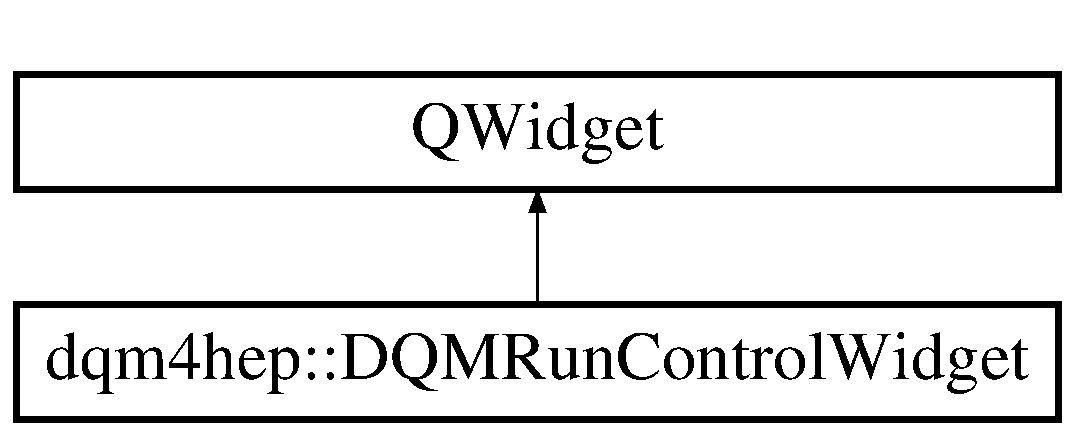
\includegraphics[height=2.000000cm]{classdqm4hep_1_1DQMRunControlWidget}
\end{center}
\end{figure}
\subsection*{Public Slots}
\begin{DoxyCompactItemize}
\item 
void {\bf start\+New\+Run} ()
\begin{DoxyCompactList}\small\item\em Start a new run. \end{DoxyCompactList}\item 
void {\bf end\+Current\+Run} ()
\begin{DoxyCompactList}\small\item\em End the current run. \end{DoxyCompactList}\item 
void {\bf add\+New\+Row} ()
\begin{DoxyCompactList}\small\item\em Add row to Table Widget. \end{DoxyCompactList}\item 
void {\bf delete\+Row} ()
\begin{DoxyCompactList}\small\item\em Add row to Table Widget. \end{DoxyCompactList}\item 
void {\bf import\+File} ()
\item 
void {\bf import\+File} (const std\+::string \&file\+Name)
\item 
void {\bf export\+File} ()
\item 
void {\bf export\+File} (const std\+::string \&file\+Name)
\end{DoxyCompactItemize}
\subsection*{Public Member Functions}
\begin{DoxyCompactItemize}
\item 
{\bf D\+Q\+M\+Run\+Control\+Widget} (D\+Q\+M\+Logger $\ast$p\+Logger=0, Q\+Widget $\ast$p\+Parent=0)
\begin{DoxyCompactList}\small\item\em Constructor with logger and parent widget (optional) \end{DoxyCompactList}\item 
{\bf $\sim$\+D\+Q\+M\+Run\+Control\+Widget} ()
\begin{DoxyCompactList}\small\item\em Destructor. \end{DoxyCompactList}\item 
void {\bf set\+Run\+Control\+Name} (const Q\+String \&name)
\begin{DoxyCompactList}\small\item\em Set the run control name. \end{DoxyCompactList}\item 
Q\+String {\bf get\+Run\+Control\+Name} () const 
\begin{DoxyCompactList}\small\item\em Get the run control name. \end{DoxyCompactList}\item 
Q\+String {\bf get\+Detector\+Name} () const 
\begin{DoxyCompactList}\small\item\em Get the detector name. \end{DoxyCompactList}\item 
Q\+String {\bf get\+Description} () const 
\begin{DoxyCompactList}\small\item\em Get the run description as displayed on the widget. \end{DoxyCompactList}\item 
Q\+String {\bf get\+Start\+Time} () const 
\begin{DoxyCompactList}\small\item\em Get the start time of the current run in h\+:m\+:s string format. \end{DoxyCompactList}\item 
Q\+String {\bf get\+End\+Time} () const 
\begin{DoxyCompactList}\small\item\em Get the end time of the last run in h\+:m\+:s string format. \end{DoxyCompactList}\item 
Q\+String {\bf get\+Status} () const 
\begin{DoxyCompactList}\small\item\em Get the run control status (running or stopped) as a string. \end{DoxyCompactList}\item 
int {\bf get\+Run\+Number} () const 
\begin{DoxyCompactList}\small\item\em Get the run number as shown on the spin box. \end{DoxyCompactList}\item 
void {\bf start} ()
\begin{DoxyCompactList}\small\item\em Start the run control service. \end{DoxyCompactList}\item 
void {\bf stop} ()
\begin{DoxyCompactList}\small\item\em Stop the run control service. \end{DoxyCompactList}\end{DoxyCompactItemize}
\subsection*{Private Attributes}
\begin{DoxyCompactItemize}
\item 
Q\+Group\+Box $\ast$ {\bf m\+\_\+p\+Run\+Action\+Group\+Box}
\item 
Q\+Line\+Edit $\ast$ {\bf m\+\_\+p\+Detector\+Name\+Edit}
\item 
Q\+Text\+Edit $\ast$ {\bf m\+\_\+p\+Run\+Description\+Text\+Edit}
\item 
Q\+Table\+Widget $\ast$ {\bf m\+\_\+p\+Run\+Parameters\+Table\+Widget}
\item 
Q\+Push\+Button $\ast$ {\bf m\+\_\+p\+Add\+Parameter\+Button}
\item 
Q\+Push\+Button $\ast$ {\bf m\+\_\+p\+Delete\+Parameter\+Button}
\item 
Q\+Push\+Button $\ast$ {\bf m\+\_\+p\+Start\+Of\+Run\+Button}
\item 
Q\+Push\+Button $\ast$ {\bf m\+\_\+p\+End\+Of\+Run\+Button}
\item 
Q\+Spin\+Box $\ast$ {\bf m\+\_\+p\+Run\+Number\+Spin\+Box}
\item 
Q\+Label $\ast$ {\bf m\+\_\+p\+Run\+Number\+Label}
\item 
Q\+Label $\ast$ {\bf m\+\_\+p\+Run\+State\+Label}
\item 
Q\+Label $\ast$ {\bf m\+\_\+p\+Run\+Start\+Time\+Label}
\item 
Q\+Label $\ast$ {\bf m\+\_\+p\+Run\+End\+Time\+Label}
\item 
D\+Q\+M\+Run\+Control\+Service $\ast$ {\bf m\+\_\+p\+Run\+Control\+Service}
\item 
D\+Q\+M\+Logger $\ast$ {\bf m\+\_\+p\+Logger}
\end{DoxyCompactItemize}


\subsection{Detailed Description}
\doxyref{D\+Q\+M\+Run\+Control\+Widget}{p.}{classdqm4hep_1_1DQMRunControlWidget} class. 

A Q\+Group\+Box widget providing the run control commands for dqm 

Definition at line 53 of file D\+Q\+M\+Run\+Control\+Widget.\+h.



\subsection{Constructor \& Destructor Documentation}
\index{dqm4hep\+::\+D\+Q\+M\+Run\+Control\+Widget@{dqm4hep\+::\+D\+Q\+M\+Run\+Control\+Widget}!D\+Q\+M\+Run\+Control\+Widget@{D\+Q\+M\+Run\+Control\+Widget}}
\index{D\+Q\+M\+Run\+Control\+Widget@{D\+Q\+M\+Run\+Control\+Widget}!dqm4hep\+::\+D\+Q\+M\+Run\+Control\+Widget@{dqm4hep\+::\+D\+Q\+M\+Run\+Control\+Widget}}
\subsubsection[{D\+Q\+M\+Run\+Control\+Widget}]{\setlength{\rightskip}{0pt plus 5cm}dqm4hep\+::\+D\+Q\+M\+Run\+Control\+Widget\+::\+D\+Q\+M\+Run\+Control\+Widget (
\begin{DoxyParamCaption}
\item[{D\+Q\+M\+Logger $\ast$}]{p\+Logger = {\ttfamily 0}, }
\item[{Q\+Widget $\ast$}]{p\+Parent = {\ttfamily 0}}
\end{DoxyParamCaption}
)}\label{classdqm4hep_1_1DQMRunControlWidget_aef5aeb2caccf0a0cb0dc5896bb8b5caa}


Constructor with logger and parent widget (optional) 



Definition at line 47 of file D\+Q\+M\+Run\+Control\+Widget.\+cc.



References add\+New\+Row(), delete\+Row(), end\+Current\+Run(), m\+\_\+p\+Add\+Parameter\+Button, m\+\_\+p\+Delete\+Parameter\+Button, m\+\_\+p\+Detector\+Name\+Edit, m\+\_\+p\+End\+Of\+Run\+Button, m\+\_\+p\+Run\+Action\+Group\+Box, m\+\_\+p\+Run\+Control\+Service, m\+\_\+p\+Run\+Description\+Text\+Edit, m\+\_\+p\+Run\+End\+Time\+Label, m\+\_\+p\+Run\+Number\+Label, m\+\_\+p\+Run\+Number\+Spin\+Box, m\+\_\+p\+Run\+Parameters\+Table\+Widget, m\+\_\+p\+Run\+Start\+Time\+Label, m\+\_\+p\+Run\+State\+Label, m\+\_\+p\+Start\+Of\+Run\+Button, and start\+New\+Run().


\begin{DoxyCode}
47                                                                              :
48     QWidget(pParent),
49     m_pLogger(pLogger)
50 \{
51     \textcolor{comment}{// Main layout}
52     QVBoxLayout *pRunControlLayout = \textcolor{keyword}{new} QVBoxLayout();
53     setLayout(pRunControlLayout);
54 
55     \textcolor{comment}{// Run action group box}
56     m_pRunActionGroupBox = \textcolor{keyword}{new} QGroupBox(\textcolor{stringliteral}{"Run info"}, \textcolor{keyword}{this});
57     QFormLayout *pRunActionLayout = \textcolor{keyword}{new} QFormLayout();
58     pRunActionLayout->setFieldGrowthPolicy(QFormLayout::ExpandingFieldsGrow);
59     m_pRunActionGroupBox->setLayout(pRunActionLayout);
60     pRunControlLayout->addWidget(m_pRunActionGroupBox);
61 
62     m_pRunNumberSpinBox = \textcolor{keyword}{new} QSpinBox();
63     m_pRunNumberSpinBox->setMinimum(1);
64     m_pRunNumberSpinBox->setMaximum(std::numeric\_limits<int>::max());
65     m_pRunNumberSpinBox->setSizePolicy(QSizePolicy(QSizePolicy::Expanding, QSizePolicy::Expanding));
66     m_pRunNumberSpinBox->setAlignment(Qt::AlignRight);
67     pRunActionLayout->addRow(\textcolor{stringliteral}{"Run number : "}, m_pRunNumberSpinBox);
68 
69     m_pRunDescriptionTextEdit = \textcolor{keyword}{new} QTextEdit();
70     pRunActionLayout->addRow(\textcolor{stringliteral}{"Run description : "}, m_pRunDescriptionTextEdit);
71 
72     m_pRunParametersTableWidget = \textcolor{keyword}{new} QTableWidget(0,2);
73     m_pRunParametersTableWidget->setSelectionMode(QTableWidget::ExtendedSelection);
74 
75 
76     m_pRunParametersTableWidget->setHorizontalHeaderLabels(QStringList() << \textcolor{stringliteral}{"Parameter"} << \textcolor{stringliteral}{"Value"});
77     QHeaderView* pHeaderView = m_pRunParametersTableWidget->horizontalHeader();
78     pHeaderView->setResizeMode(QHeaderView::Stretch);
79     pRunActionLayout->addRow(\textcolor{stringliteral}{"Run Parameters : "}, m_pRunParametersTableWidget);
80 
81     QWidget *pParameterButtonWidget = \textcolor{keyword}{new} QWidget();
82     QHBoxLayout *pParameterButtonLayout = \textcolor{keyword}{new} QHBoxLayout();
83     pParameterButtonWidget->setLayout(pParameterButtonLayout);
84 
85     pParameterButtonLayout->addSpacerItem(\textcolor{keyword}{new} QSpacerItem(1, 0, QSizePolicy::Expanding, 
      QSizePolicy::Minimum));
86 
87     m_pAddParameterButton = \textcolor{keyword}{new} QPushButton(\textcolor{stringliteral}{"Add Parameter"});
88     pParameterButtonLayout->addWidget(m_pAddParameterButton);
89 
90     connect(m_pAddParameterButton, SIGNAL(clicked()), \textcolor{keyword}{this}, SLOT(addNewRow()));
91 
92     m_pDeleteParameterButton = \textcolor{keyword}{new} QPushButton(\textcolor{stringliteral}{"Delete Parameter"});
93     pParameterButtonLayout->addWidget(m_pDeleteParameterButton);
94     connect(m_pDeleteParameterButton, SIGNAL(clicked()), \textcolor{keyword}{this}, SLOT(deleteRow()));
95     pRunActionLayout->addWidget(pParameterButtonWidget);
96 
97     m_pDetectorNameEdit = \textcolor{keyword}{new} QLineEdit();
98     pRunActionLayout->addRow(\textcolor{stringliteral}{"Detector name : "}, m_pDetectorNameEdit);
99 
100 
101 
102     QWidget *pRunActionButtonWidget = \textcolor{keyword}{new} QWidget();
103     QHBoxLayout *pRunActionButtonLayout = \textcolor{keyword}{new} QHBoxLayout();
104     pRunActionButtonWidget->setLayout(pRunActionButtonLayout);
105 
106     QFont buttonFont;
107     buttonFont.setWeight(QFont::Bold);
108     buttonFont.setPointSize(15);
109 
110     m_pStartOfRunButton = \textcolor{keyword}{new} QPushButton(\textcolor{stringliteral}{"Start run"});
111     m_pStartOfRunButton->setMinimumHeight(70);
112     m_pStartOfRunButton->setFont(buttonFont);
113     pRunActionButtonLayout->addWidget(m_pStartOfRunButton);
114 
115     m_pEndOfRunButton = \textcolor{keyword}{new} QPushButton(\textcolor{stringliteral}{"End run"});
116     pRunActionButtonLayout->addWidget(m_pEndOfRunButton);
117     m_pEndOfRunButton->setMinimumHeight(70);
118     m_pEndOfRunButton->setFont(buttonFont);
119     m_pEndOfRunButton->setEnabled(\textcolor{keyword}{false});
120 
121     pRunControlLayout->addWidget(pRunActionButtonWidget);
122 
123     m_pRunControlService = \textcolor{keyword}{new} DQMRunControlService();
124 
125     \textcolor{comment}{// run status group box}
126     QGroupBox *pRunStatusGroupBox = \textcolor{keyword}{new} QGroupBox(\textcolor{stringliteral}{"Run status"});
127     QGridLayout *pRunStatusLayout = \textcolor{keyword}{new} QGridLayout();
128     pRunStatusGroupBox->setLayout(pRunStatusLayout);
129     pRunControlLayout->addWidget(pRunStatusGroupBox);
130 
131     pRunStatusLayout->addWidget(\textcolor{keyword}{new} QLabel(\textcolor{stringliteral}{"Run number"}), 0, 0, Qt::AlignCenter);
132     pRunStatusLayout->addWidget(\textcolor{keyword}{new} QLabel(\textcolor{stringliteral}{"Run state"}), 0, 1, Qt::AlignCenter);
133     pRunStatusLayout->addWidget(\textcolor{keyword}{new} QLabel(\textcolor{stringliteral}{"Started at"}), 0, 2, Qt::AlignCenter);
134     pRunStatusLayout->addWidget(\textcolor{keyword}{new} QLabel(\textcolor{stringliteral}{"Ended at"}), 0, 3, Qt::AlignCenter);
135 
136     m_pRunNumberLabel = \textcolor{keyword}{new} QLabel(QString(\textcolor{stringliteral}{"<b>NONE</b>"}));
137     pRunStatusLayout->addWidget(m_pRunNumberLabel, 1, 0, Qt::AlignCenter);
138     m_pRunStateLabel = \textcolor{keyword}{new} QLabel(stateToString(m_pRunControlService->getRunState()).c\_str());
139     pRunStatusLayout->addWidget(m_pRunStateLabel, 1, 1, Qt::AlignCenter);
140     m_pRunStartTimeLabel = \textcolor{keyword}{new} QLabel(\textcolor{stringliteral}{"NONE"});
141     pRunStatusLayout->addWidget(m_pRunStartTimeLabel, 1, 2, Qt::AlignCenter);
142     m_pRunEndTimeLabel = \textcolor{keyword}{new} QLabel(\textcolor{stringliteral}{"NONE"});
143     pRunStatusLayout->addWidget(m_pRunEndTimeLabel, 1, 3, Qt::AlignCenter);
144 
145     connect(m_pStartOfRunButton, SIGNAL(clicked()), \textcolor{keyword}{this}, SLOT(startNewRun()));
146     connect(m_pEndOfRunButton, SIGNAL(clicked()), \textcolor{keyword}{this}, SLOT(endCurrentRun()));
147 \}
\end{DoxyCode}
\index{dqm4hep\+::\+D\+Q\+M\+Run\+Control\+Widget@{dqm4hep\+::\+D\+Q\+M\+Run\+Control\+Widget}!````~D\+Q\+M\+Run\+Control\+Widget@{$\sim$\+D\+Q\+M\+Run\+Control\+Widget}}
\index{````~D\+Q\+M\+Run\+Control\+Widget@{$\sim$\+D\+Q\+M\+Run\+Control\+Widget}!dqm4hep\+::\+D\+Q\+M\+Run\+Control\+Widget@{dqm4hep\+::\+D\+Q\+M\+Run\+Control\+Widget}}
\subsubsection[{$\sim$\+D\+Q\+M\+Run\+Control\+Widget}]{\setlength{\rightskip}{0pt plus 5cm}dqm4hep\+::\+D\+Q\+M\+Run\+Control\+Widget\+::$\sim$\+D\+Q\+M\+Run\+Control\+Widget (
\begin{DoxyParamCaption}
{}
\end{DoxyParamCaption}
)}\label{classdqm4hep_1_1DQMRunControlWidget_a54dc53956ba410f0f7e4f25b07b3caaf}


Destructor. 



Definition at line 151 of file D\+Q\+M\+Run\+Control\+Widget.\+cc.



References m\+\_\+p\+Run\+Control\+Service.


\begin{DoxyCode}
152 \{
153     \textcolor{keywordflow}{if}(m_pRunControlService->isRunning())
154         m_pRunControlService->stop();
155 
156     \textcolor{keyword}{delete} m_pRunControlService;
157 \}
\end{DoxyCode}


\subsection{Member Function Documentation}
\index{dqm4hep\+::\+D\+Q\+M\+Run\+Control\+Widget@{dqm4hep\+::\+D\+Q\+M\+Run\+Control\+Widget}!add\+New\+Row@{add\+New\+Row}}
\index{add\+New\+Row@{add\+New\+Row}!dqm4hep\+::\+D\+Q\+M\+Run\+Control\+Widget@{dqm4hep\+::\+D\+Q\+M\+Run\+Control\+Widget}}
\subsubsection[{add\+New\+Row}]{\setlength{\rightskip}{0pt plus 5cm}void dqm4hep\+::\+D\+Q\+M\+Run\+Control\+Widget\+::add\+New\+Row (
\begin{DoxyParamCaption}
{}
\end{DoxyParamCaption}
)\hspace{0.3cm}{\ttfamily [slot]}}\label{classdqm4hep_1_1DQMRunControlWidget_a10368edd077245a48c569f05c9e75af8}


Add row to Table Widget. 



Definition at line 392 of file D\+Q\+M\+Run\+Control\+Widget.\+cc.



References m\+\_\+p\+Run\+Parameters\+Table\+Widget.



Referenced by D\+Q\+M\+Run\+Control\+Widget().


\begin{DoxyCode}
393 \{
394     m_pRunParametersTableWidget->insertRow(m_pRunParametersTableWidget->rowCount());
395 \}
\end{DoxyCode}
\index{dqm4hep\+::\+D\+Q\+M\+Run\+Control\+Widget@{dqm4hep\+::\+D\+Q\+M\+Run\+Control\+Widget}!delete\+Row@{delete\+Row}}
\index{delete\+Row@{delete\+Row}!dqm4hep\+::\+D\+Q\+M\+Run\+Control\+Widget@{dqm4hep\+::\+D\+Q\+M\+Run\+Control\+Widget}}
\subsubsection[{delete\+Row}]{\setlength{\rightskip}{0pt plus 5cm}void dqm4hep\+::\+D\+Q\+M\+Run\+Control\+Widget\+::delete\+Row (
\begin{DoxyParamCaption}
{}
\end{DoxyParamCaption}
)\hspace{0.3cm}{\ttfamily [slot]}}\label{classdqm4hep_1_1DQMRunControlWidget_a912452db10023b3eee8c7b514a91544f}


Add row to Table Widget. 



Definition at line 398 of file D\+Q\+M\+Run\+Control\+Widget.\+cc.



References m\+\_\+p\+Run\+Parameters\+Table\+Widget.



Referenced by D\+Q\+M\+Run\+Control\+Widget().


\begin{DoxyCode}
399 \{
400     QList<QTableWidgetSelectionRange> selectedRanges = 
      m_pRunParametersTableWidget->selectedRanges();
401     \textcolor{keywordflow}{for} (\textcolor{keywordtype}{int} i = 0; i< selectedRanges.size(); i++ )
402     \{
403         \textcolor{keywordtype}{int} topRow = selectedRanges.at(i).topRow();
404         \textcolor{keywordtype}{int} botRow = selectedRanges.at(i).bottomRow();
405         \textcolor{keywordtype}{int} inc = topRow;
406         \textcolor{keywordflow}{while}(inc <= botRow)
407         \{
408             m_pRunParametersTableWidget->removeRow(topRow);
409             inc++;
410         \}
411     \}
412     m_pRunParametersTableWidget->setCurrentCell(-1,-1);
413 \}
\end{DoxyCode}
\index{dqm4hep\+::\+D\+Q\+M\+Run\+Control\+Widget@{dqm4hep\+::\+D\+Q\+M\+Run\+Control\+Widget}!end\+Current\+Run@{end\+Current\+Run}}
\index{end\+Current\+Run@{end\+Current\+Run}!dqm4hep\+::\+D\+Q\+M\+Run\+Control\+Widget@{dqm4hep\+::\+D\+Q\+M\+Run\+Control\+Widget}}
\subsubsection[{end\+Current\+Run}]{\setlength{\rightskip}{0pt plus 5cm}void dqm4hep\+::\+D\+Q\+M\+Run\+Control\+Widget\+::end\+Current\+Run (
\begin{DoxyParamCaption}
{}
\end{DoxyParamCaption}
)\hspace{0.3cm}{\ttfamily [slot]}}\label{classdqm4hep_1_1DQMRunControlWidget_a6236e6d9a7cc554013f16b41fcbfe811}


End the current run. 



Definition at line 358 of file D\+Q\+M\+Run\+Control\+Widget.\+cc.



References m\+\_\+p\+End\+Of\+Run\+Button, m\+\_\+p\+Logger, m\+\_\+p\+Run\+Control\+Service, m\+\_\+p\+Run\+End\+Time\+Label, m\+\_\+p\+Run\+State\+Label, and m\+\_\+p\+Start\+Of\+Run\+Button.



Referenced by D\+Q\+M\+Run\+Control\+Widget().


\begin{DoxyCode}
359 \{
360     \textcolor{keywordflow}{if}(m_pRunControlService->isRunning())
361     \{
362         \textcolor{keywordflow}{try}
363         \{
364             \textcolor{keywordflow}{if}(m_pLogger)
365                 m_pLogger->log(MESSAGE, \textcolor{stringliteral}{"Stopping current run"});
366 
367             THROW\_RESULT\_IF(STATUS\_CODE\_SUCCESS, !=, m_pRunControlService->endCurrentRun());
368 
369             time\_t endTime = time(NULL);
370             std::string startTimeStdStr;
371             DQMCoreTool::timeToHMS(endTime, startTimeStdStr);
372 
373             m_pRunStateLabel->setText(stateToString(m_pRunControlService->getRunState()).c\_str());
374             m_pRunEndTimeLabel->setText(startTimeStdStr.c\_str());
375         \}
376         \textcolor{keywordflow}{catch}(StatusCodeException &exception)
377         \{
378             \textcolor{keywordflow}{if}(m_pLogger)
379                 m_pLogger->log(ERROR, \textcolor{stringliteral}{"Couldn't end current run : "} + exception.toString());
380             \textcolor{keywordflow}{return};
381         \}
382     \}
383     \textcolor{keywordflow}{else}
384         \textcolor{keywordflow}{return};
385 
386     m_pStartOfRunButton->setEnabled(\textcolor{keyword}{true});
387     m_pEndOfRunButton->setEnabled(\textcolor{keyword}{false});
388 \}
\end{DoxyCode}
\index{dqm4hep\+::\+D\+Q\+M\+Run\+Control\+Widget@{dqm4hep\+::\+D\+Q\+M\+Run\+Control\+Widget}!export\+File@{export\+File}}
\index{export\+File@{export\+File}!dqm4hep\+::\+D\+Q\+M\+Run\+Control\+Widget@{dqm4hep\+::\+D\+Q\+M\+Run\+Control\+Widget}}
\subsubsection[{export\+File}]{\setlength{\rightskip}{0pt plus 5cm}void dqm4hep\+::\+D\+Q\+M\+Run\+Control\+Widget\+::export\+File (
\begin{DoxyParamCaption}
{}
\end{DoxyParamCaption}
)\hspace{0.3cm}{\ttfamily [slot]}}\label{classdqm4hep_1_1DQMRunControlWidget_a4e3b0815f89bbc70dc4bcfc4516e583b}


Definition at line 513 of file D\+Q\+M\+Run\+Control\+Widget.\+cc.


\begin{DoxyCode}
514 \{
515     QString fileName = QFileDialog::getSaveFileName(\textcolor{keyword}{this}, \textcolor{stringliteral}{"Export"}, \textcolor{stringliteral}{""}, \textcolor{stringliteral}{"XML (*.xml)"});
516     exportFile(fileName.toStdString());
517 \}
\end{DoxyCode}
\index{dqm4hep\+::\+D\+Q\+M\+Run\+Control\+Widget@{dqm4hep\+::\+D\+Q\+M\+Run\+Control\+Widget}!export\+File@{export\+File}}
\index{export\+File@{export\+File}!dqm4hep\+::\+D\+Q\+M\+Run\+Control\+Widget@{dqm4hep\+::\+D\+Q\+M\+Run\+Control\+Widget}}
\subsubsection[{export\+File}]{\setlength{\rightskip}{0pt plus 5cm}void dqm4hep\+::\+D\+Q\+M\+Run\+Control\+Widget\+::export\+File (
\begin{DoxyParamCaption}
\item[{const std\+::string \&}]{file\+Name}
\end{DoxyParamCaption}
)\hspace{0.3cm}{\ttfamily [slot]}}\label{classdqm4hep_1_1DQMRunControlWidget_a68ce0640aaf73160645112a5bfc94103}


Definition at line 521 of file D\+Q\+M\+Run\+Control\+Widget.\+cc.



References m\+\_\+p\+Detector\+Name\+Edit, m\+\_\+p\+Run\+Description\+Text\+Edit, m\+\_\+p\+Run\+Number\+Spin\+Box, and m\+\_\+p\+Run\+Parameters\+Table\+Widget.


\begin{DoxyCode}
522 \{
523   TiXmlDocument document;
524 
525   TiXmlDeclaration *pDeclaration = \textcolor{keyword}{new} TiXmlDeclaration( \textcolor{stringliteral}{"1.0"}, \textcolor{stringliteral}{""}, \textcolor{stringliteral}{""} );
526   document.LinkEndChild(pDeclaration);
527 
528   TiXmlElement *pRootElement = \textcolor{keyword}{new} TiXmlElement(\textcolor{stringliteral}{"dqm4hep"});
529   document.LinkEndChild(pRootElement);
530 
531   TiXmlElement *pRunInfoElement = \textcolor{keyword}{new} TiXmlElement(\textcolor{stringliteral}{"runinfo"});
532   pRootElement->LinkEndChild(pRunInfoElement);
533 
534   TiXmlElement *pRunNumberElement = \textcolor{keyword}{new} TiXmlElement(\textcolor{stringliteral}{"runnumber"});
535   pRunNumberElement->SetAttribute(\textcolor{stringliteral}{"value"}, static\_cast<int>(m_pRunNumberSpinBox->value()));
536   pRunInfoElement->LinkEndChild(pRunNumberElement);
537 
538   TiXmlElement *pDetectorElement = \textcolor{keyword}{new} TiXmlElement(\textcolor{stringliteral}{"detector"});
539   pDetectorElement->SetAttribute(\textcolor{stringliteral}{"name"}, m_pDetectorNameEdit->text().toStdString());
540   pRunInfoElement->LinkEndChild(pDetectorElement);
541 
542   TiXmlElement *pDescriptionElement = \textcolor{keyword}{new} TiXmlElement(\textcolor{stringliteral}{"description"});
543   pDescriptionElement->SetAttribute(\textcolor{stringliteral}{"value"}, m_pRunDescriptionTextEdit->toPlainText().toStdString());
544   pRunInfoElement->LinkEndChild(pDescriptionElement);
545 
546 
547     \textcolor{keywordflow}{if}(m_pRunParametersTableWidget->rowCount() > 0)
548     \{
549       TiXmlElement *pParametersElement = \textcolor{keyword}{new} TiXmlElement(\textcolor{stringliteral}{"parameters"});
550       pRunInfoElement->LinkEndChild(pParametersElement);
551 
552         \textcolor{keywordflow}{for}(\textcolor{keywordtype}{unsigned} \textcolor{keywordtype}{int} i=0 ; i<m_pRunParametersTableWidget->rowCount() ; i++)
553         \{
554             QTableWidgetItem *pKeyItem = m_pRunParametersTableWidget->item(i, 0);
555             QTableWidgetItem *pValueItem = m_pRunParametersTableWidget->item(i, 1);
556 
557             \textcolor{keywordflow}{if}(!pKeyItem || !pValueItem)
558                 \textcolor{keywordflow}{continue};
559 
560           TiXmlElement *pParameterElement = \textcolor{keyword}{new} TiXmlElement(\textcolor{stringliteral}{"parameter"});
561           pParameterElement->SetAttribute(\textcolor{stringliteral}{"name"}, pKeyItem->text().toStdString());
562           pParameterElement->SetAttribute(\textcolor{stringliteral}{"value"}, pValueItem->text().toStdString());
563           pParametersElement->LinkEndChild(pParameterElement);
564         \}
565     \}
566 
567   document.SaveFile(fileName);
568 \}
\end{DoxyCode}
\index{dqm4hep\+::\+D\+Q\+M\+Run\+Control\+Widget@{dqm4hep\+::\+D\+Q\+M\+Run\+Control\+Widget}!get\+Description@{get\+Description}}
\index{get\+Description@{get\+Description}!dqm4hep\+::\+D\+Q\+M\+Run\+Control\+Widget@{dqm4hep\+::\+D\+Q\+M\+Run\+Control\+Widget}}
\subsubsection[{get\+Description}]{\setlength{\rightskip}{0pt plus 5cm}Q\+String dqm4hep\+::\+D\+Q\+M\+Run\+Control\+Widget\+::get\+Description (
\begin{DoxyParamCaption}
{}
\end{DoxyParamCaption}
) const}\label{classdqm4hep_1_1DQMRunControlWidget_a0b28183dd7c6078315e32341f2a0585a}


Get the run description as displayed on the widget. 



Definition at line 256 of file D\+Q\+M\+Run\+Control\+Widget.\+cc.



References m\+\_\+p\+Run\+Description\+Text\+Edit.



Referenced by start\+New\+Run().


\begin{DoxyCode}
257 \{
258     \textcolor{keywordflow}{return} m_pRunDescriptionTextEdit->toPlainText();
259 \}
\end{DoxyCode}
\index{dqm4hep\+::\+D\+Q\+M\+Run\+Control\+Widget@{dqm4hep\+::\+D\+Q\+M\+Run\+Control\+Widget}!get\+Detector\+Name@{get\+Detector\+Name}}
\index{get\+Detector\+Name@{get\+Detector\+Name}!dqm4hep\+::\+D\+Q\+M\+Run\+Control\+Widget@{dqm4hep\+::\+D\+Q\+M\+Run\+Control\+Widget}}
\subsubsection[{get\+Detector\+Name}]{\setlength{\rightskip}{0pt plus 5cm}Q\+String dqm4hep\+::\+D\+Q\+M\+Run\+Control\+Widget\+::get\+Detector\+Name (
\begin{DoxyParamCaption}
{}
\end{DoxyParamCaption}
) const}\label{classdqm4hep_1_1DQMRunControlWidget_abf2336fe28083be3fa9f669f2dcb1da6}


Get the detector name. 



Definition at line 249 of file D\+Q\+M\+Run\+Control\+Widget.\+cc.



References m\+\_\+p\+Detector\+Name\+Edit.



Referenced by start\+New\+Run().


\begin{DoxyCode}
250 \{
251     \textcolor{keywordflow}{return} m_pDetectorNameEdit->text();
252 \}
\end{DoxyCode}
\index{dqm4hep\+::\+D\+Q\+M\+Run\+Control\+Widget@{dqm4hep\+::\+D\+Q\+M\+Run\+Control\+Widget}!get\+End\+Time@{get\+End\+Time}}
\index{get\+End\+Time@{get\+End\+Time}!dqm4hep\+::\+D\+Q\+M\+Run\+Control\+Widget@{dqm4hep\+::\+D\+Q\+M\+Run\+Control\+Widget}}
\subsubsection[{get\+End\+Time}]{\setlength{\rightskip}{0pt plus 5cm}Q\+String dqm4hep\+::\+D\+Q\+M\+Run\+Control\+Widget\+::get\+End\+Time (
\begin{DoxyParamCaption}
{}
\end{DoxyParamCaption}
) const}\label{classdqm4hep_1_1DQMRunControlWidget_a4938f0204bf35f5c3eb0032f1cbd7940}


Get the end time of the last run in h\+:m\+:s string format. 

Returns an empty string if running 

Definition at line 270 of file D\+Q\+M\+Run\+Control\+Widget.\+cc.


\begin{DoxyCode}
271 \{
272     \textcolor{keywordflow}{return} QString(\textcolor{stringliteral}{""});
273 \}
\end{DoxyCode}
\index{dqm4hep\+::\+D\+Q\+M\+Run\+Control\+Widget@{dqm4hep\+::\+D\+Q\+M\+Run\+Control\+Widget}!get\+Run\+Control\+Name@{get\+Run\+Control\+Name}}
\index{get\+Run\+Control\+Name@{get\+Run\+Control\+Name}!dqm4hep\+::\+D\+Q\+M\+Run\+Control\+Widget@{dqm4hep\+::\+D\+Q\+M\+Run\+Control\+Widget}}
\subsubsection[{get\+Run\+Control\+Name}]{\setlength{\rightskip}{0pt plus 5cm}Q\+String dqm4hep\+::\+D\+Q\+M\+Run\+Control\+Widget\+::get\+Run\+Control\+Name (
\begin{DoxyParamCaption}
{}
\end{DoxyParamCaption}
) const}\label{classdqm4hep_1_1DQMRunControlWidget_af7fc667c5dd2e7d5955156e12ffe08eb}


Get the run control name. 



Definition at line 235 of file D\+Q\+M\+Run\+Control\+Widget.\+cc.



References m\+\_\+p\+Run\+Control\+Service.



Referenced by start().


\begin{DoxyCode}
236 \{
237     \textcolor{keywordflow}{return} QString(m_pRunControlService->getRunControlName().c\_str());
238 \}
\end{DoxyCode}
\index{dqm4hep\+::\+D\+Q\+M\+Run\+Control\+Widget@{dqm4hep\+::\+D\+Q\+M\+Run\+Control\+Widget}!get\+Run\+Number@{get\+Run\+Number}}
\index{get\+Run\+Number@{get\+Run\+Number}!dqm4hep\+::\+D\+Q\+M\+Run\+Control\+Widget@{dqm4hep\+::\+D\+Q\+M\+Run\+Control\+Widget}}
\subsubsection[{get\+Run\+Number}]{\setlength{\rightskip}{0pt plus 5cm}int dqm4hep\+::\+D\+Q\+M\+Run\+Control\+Widget\+::get\+Run\+Number (
\begin{DoxyParamCaption}
{}
\end{DoxyParamCaption}
) const}\label{classdqm4hep_1_1DQMRunControlWidget_ad2c78e488d3d2d08082fb962fdf138d8}


Get the run number as shown on the spin box. 



Definition at line 284 of file D\+Q\+M\+Run\+Control\+Widget.\+cc.



References m\+\_\+p\+Run\+Number\+Spin\+Box.


\begin{DoxyCode}
285 \{
286     \textcolor{keywordflow}{return} m_pRunNumberSpinBox->value();
287 \}
\end{DoxyCode}
\index{dqm4hep\+::\+D\+Q\+M\+Run\+Control\+Widget@{dqm4hep\+::\+D\+Q\+M\+Run\+Control\+Widget}!get\+Start\+Time@{get\+Start\+Time}}
\index{get\+Start\+Time@{get\+Start\+Time}!dqm4hep\+::\+D\+Q\+M\+Run\+Control\+Widget@{dqm4hep\+::\+D\+Q\+M\+Run\+Control\+Widget}}
\subsubsection[{get\+Start\+Time}]{\setlength{\rightskip}{0pt plus 5cm}Q\+String dqm4hep\+::\+D\+Q\+M\+Run\+Control\+Widget\+::get\+Start\+Time (
\begin{DoxyParamCaption}
{}
\end{DoxyParamCaption}
) const}\label{classdqm4hep_1_1DQMRunControlWidget_af45802af5ff6bf92506c2796e127da07}


Get the start time of the current run in h\+:m\+:s string format. 

Returns an empty string if not running 

Definition at line 263 of file D\+Q\+M\+Run\+Control\+Widget.\+cc.


\begin{DoxyCode}
264 \{
265     \textcolor{keywordflow}{return} QString(\textcolor{stringliteral}{""});
266 \}
\end{DoxyCode}
\index{dqm4hep\+::\+D\+Q\+M\+Run\+Control\+Widget@{dqm4hep\+::\+D\+Q\+M\+Run\+Control\+Widget}!get\+Status@{get\+Status}}
\index{get\+Status@{get\+Status}!dqm4hep\+::\+D\+Q\+M\+Run\+Control\+Widget@{dqm4hep\+::\+D\+Q\+M\+Run\+Control\+Widget}}
\subsubsection[{get\+Status}]{\setlength{\rightskip}{0pt plus 5cm}Q\+String dqm4hep\+::\+D\+Q\+M\+Run\+Control\+Widget\+::get\+Status (
\begin{DoxyParamCaption}
{}
\end{DoxyParamCaption}
) const}\label{classdqm4hep_1_1DQMRunControlWidget_a48fd9a2129a8796ccf4d5c9fc01c70b3}


Get the run control status (running or stopped) as a string. 



Definition at line 277 of file D\+Q\+M\+Run\+Control\+Widget.\+cc.



References m\+\_\+p\+Run\+Control\+Service.


\begin{DoxyCode}
278 \{
279     \textcolor{keywordflow}{return} QString(stateToString(m_pRunControlService->getRunState()).c\_str());
280 \}
\end{DoxyCode}
\index{dqm4hep\+::\+D\+Q\+M\+Run\+Control\+Widget@{dqm4hep\+::\+D\+Q\+M\+Run\+Control\+Widget}!import\+File@{import\+File}}
\index{import\+File@{import\+File}!dqm4hep\+::\+D\+Q\+M\+Run\+Control\+Widget@{dqm4hep\+::\+D\+Q\+M\+Run\+Control\+Widget}}
\subsubsection[{import\+File}]{\setlength{\rightskip}{0pt plus 5cm}void dqm4hep\+::\+D\+Q\+M\+Run\+Control\+Widget\+::import\+File (
\begin{DoxyParamCaption}
{}
\end{DoxyParamCaption}
)\hspace{0.3cm}{\ttfamily [slot]}}\label{classdqm4hep_1_1DQMRunControlWidget_a062f29e369c4323d85076e7706d9adbf}


Definition at line 417 of file D\+Q\+M\+Run\+Control\+Widget.\+cc.


\begin{DoxyCode}
418 \{
419     QString fileName = QFileDialog::getOpenFileName(\textcolor{keyword}{this}, \textcolor{stringliteral}{"Import"}, \textcolor{stringliteral}{""}, \textcolor{stringliteral}{"Xml (*.xml)"});
420     this->importFile(fileName.toStdString());
421 \}
\end{DoxyCode}
\index{dqm4hep\+::\+D\+Q\+M\+Run\+Control\+Widget@{dqm4hep\+::\+D\+Q\+M\+Run\+Control\+Widget}!import\+File@{import\+File}}
\index{import\+File@{import\+File}!dqm4hep\+::\+D\+Q\+M\+Run\+Control\+Widget@{dqm4hep\+::\+D\+Q\+M\+Run\+Control\+Widget}}
\subsubsection[{import\+File}]{\setlength{\rightskip}{0pt plus 5cm}void dqm4hep\+::\+D\+Q\+M\+Run\+Control\+Widget\+::import\+File (
\begin{DoxyParamCaption}
\item[{const std\+::string \&}]{file\+Name}
\end{DoxyParamCaption}
)\hspace{0.3cm}{\ttfamily [slot]}}\label{classdqm4hep_1_1DQMRunControlWidget_ac62280dadb6f8d1fbd7e357c9071147b}


Definition at line 425 of file D\+Q\+M\+Run\+Control\+Widget.\+cc.



References m\+\_\+p\+Detector\+Name\+Edit, m\+\_\+p\+Run\+Description\+Text\+Edit, m\+\_\+p\+Run\+Number\+Spin\+Box, and m\+\_\+p\+Run\+Parameters\+Table\+Widget.


\begin{DoxyCode}
426 \{
427     TiXmlDocument xmlDocument(fileName);
428 
429     \textcolor{keywordflow}{if} (!xmlDocument.LoadFile())
430     \{
431         QMessageBox::warning(\textcolor{keyword}{this}, \textcolor{stringliteral}{"Warning"}, \textcolor{stringliteral}{"Invalid xml file"});
432         \textcolor{keywordflow}{return};
433     \}
434 
435     \textcolor{keyword}{const} TiXmlHandle xmlDocumentHandle(&xmlDocument);
436     \textcolor{keyword}{const} TiXmlHandle xmlHandle = TiXmlHandle(xmlDocumentHandle.FirstChildElement().Element());
437 
438     TiXmlElement *\textcolor{keyword}{const} pRunInfoElement = xmlHandle.FirstChildElement(\textcolor{stringliteral}{"runinfo"}).Element();
439 
440     \textcolor{keywordflow}{if}(!pRunInfoElement)
441     \{
442         QMessageBox::warning(\textcolor{keyword}{this}, \textcolor{stringliteral}{"Warning"}, \textcolor{stringliteral}{"Invalid xml file : Couldn't find <runinfo> element !"});
443         \textcolor{keywordflow}{return};
444     \}
445 
446     TiXmlHandle runInfoHandle(pRunInfoElement);
447 
448     \textcolor{keywordtype}{int} runNumber = 0;
449     std::string detectorName;
450     std::string description;
451 
452     m_pRunParametersTableWidget->clearContents();
453     \textcolor{keywordflow}{while} (m_pRunParametersTableWidget->rowCount() > 0)
454         m_pRunParametersTableWidget->removeRow(0);
455 
456     \textcolor{keywordflow}{try}
457     \{
458         TiXmlElement *\textcolor{keyword}{const} pRunNumberElement = runInfoHandle.FirstChildElement(\textcolor{stringliteral}{"runnumber"}).Element();
459         TiXmlElement *\textcolor{keyword}{const} pDetectorElement = runInfoHandle.FirstChildElement(\textcolor{stringliteral}{"detector"}).Element();
460         TiXmlElement *\textcolor{keyword}{const} pDescriptionElement = runInfoHandle.FirstChildElement(\textcolor{stringliteral}{"description"}).Element();
461         TiXmlElement *\textcolor{keyword}{const} pParametersElement = runInfoHandle.FirstChildElement(\textcolor{stringliteral}{"parameters"}).Element();
462 
463         \textcolor{keywordflow}{if}(pRunNumberElement)
464         \{
465           THROW\_RESULT\_IF(STATUS\_CODE\_SUCCESS, !=, DQMXmlHelper::getAttribute(pRunNumberElement, \textcolor{stringliteral}{"value"}, 
      runNumber));
466         \}
467 
468         \textcolor{keywordflow}{if}(pDetectorElement)
469         \{
470           THROW\_RESULT\_IF(STATUS\_CODE\_SUCCESS, !=, DQMXmlHelper::getAttribute(pDetectorElement, \textcolor{stringliteral}{"name"}, 
      detectorName));
471         \}
472 
473         \textcolor{keywordflow}{if}(pDescriptionElement)
474         \{
475           THROW\_RESULT\_IF(STATUS\_CODE\_SUCCESS, !=, DQMXmlHelper::getAttribute(pDescriptionElement, \textcolor{stringliteral}{"value"},
       description));
476         \}
477 
478         \textcolor{keywordflow}{if}(pParametersElement)
479         \{
480           TiXmlHandle parametersHandle(pParametersElement);
481 
482             \textcolor{keywordflow}{for} (TiXmlElement *pXmlElement = parametersHandle.FirstChild(\textcolor{stringliteral}{"parameter"}).Element(); NULL != 
      pXmlElement;
483                 pXmlElement = pXmlElement->NextSiblingElement(\textcolor{stringliteral}{"parameter"}))
484             \{
485               std::string name;
486               std::string value;
487 
488               THROW\_RESULT\_IF(STATUS\_CODE\_SUCCESS, !=, DQMXmlHelper::getAttribute(pXmlElement, \textcolor{stringliteral}{"name"}, name
      ));
489               THROW\_RESULT\_IF(STATUS\_CODE\_SUCCESS, !=, DQMXmlHelper::getAttribute(pXmlElement, \textcolor{stringliteral}{"value"}, 
      value));
490 
491                 \textcolor{keywordtype}{int} row = m_pRunParametersTableWidget->rowCount();
492 
493                 m_pRunParametersTableWidget->insertRow(row);
494                 m_pRunParametersTableWidget->setItem(row, 0, \textcolor{keyword}{new} QTableWidgetItem(name.c\_str()));
495                 m_pRunParametersTableWidget->setItem(row, 1, \textcolor{keyword}{new} QTableWidgetItem(value.c\_str()));
496             \}
497         \}
498     \}
499   \textcolor{keywordflow}{catch}(\textcolor{keyword}{const} StatusCodeException &exception)
500   \{
501         QMessageBox::warning(\textcolor{keyword}{this}, \textcolor{stringliteral}{"Warning"}, (\textcolor{stringliteral}{"Invalid xml file : Couldn't parse it : "} + exception.
      toString()).c\_str());
502         \textcolor{keywordflow}{return};
503   \}
504 
505     m_pRunNumberSpinBox->setValue(runNumber);
506     m_pRunDescriptionTextEdit->clear();
507     m_pRunDescriptionTextEdit->setText(description.c\_str());
508     m_pDetectorNameEdit->setText(detectorName.c\_str());
509 \}
\end{DoxyCode}
\index{dqm4hep\+::\+D\+Q\+M\+Run\+Control\+Widget@{dqm4hep\+::\+D\+Q\+M\+Run\+Control\+Widget}!set\+Run\+Control\+Name@{set\+Run\+Control\+Name}}
\index{set\+Run\+Control\+Name@{set\+Run\+Control\+Name}!dqm4hep\+::\+D\+Q\+M\+Run\+Control\+Widget@{dqm4hep\+::\+D\+Q\+M\+Run\+Control\+Widget}}
\subsubsection[{set\+Run\+Control\+Name}]{\setlength{\rightskip}{0pt plus 5cm}void dqm4hep\+::\+D\+Q\+M\+Run\+Control\+Widget\+::set\+Run\+Control\+Name (
\begin{DoxyParamCaption}
\item[{const Q\+String \&}]{name}
\end{DoxyParamCaption}
)}\label{classdqm4hep_1_1DQMRunControlWidget_aee26aded319596b9bd38eb4e3134c157}


Set the run control name. 

Can be set only if the service is not already running 

Definition at line 242 of file D\+Q\+M\+Run\+Control\+Widget.\+cc.



References m\+\_\+p\+Run\+Control\+Service.


\begin{DoxyCode}
243 \{
244     m_pRunControlService->setRunControlName(name.toStdString());
245 \}
\end{DoxyCode}
\index{dqm4hep\+::\+D\+Q\+M\+Run\+Control\+Widget@{dqm4hep\+::\+D\+Q\+M\+Run\+Control\+Widget}!start@{start}}
\index{start@{start}!dqm4hep\+::\+D\+Q\+M\+Run\+Control\+Widget@{dqm4hep\+::\+D\+Q\+M\+Run\+Control\+Widget}}
\subsubsection[{start}]{\setlength{\rightskip}{0pt plus 5cm}void dqm4hep\+::\+D\+Q\+M\+Run\+Control\+Widget\+::start (
\begin{DoxyParamCaption}
{}
\end{DoxyParamCaption}
)}\label{classdqm4hep_1_1DQMRunControlWidget_a5cdf2057d24b47919c2c02ba347260f4}


Start the run control service. 

See \doxyref{start\+New\+Run()}{p.}{classdqm4hep_1_1DQMRunControlWidget_adae54abe149e06da917663cf5dd3661b} to start a run. 

Definition at line 161 of file D\+Q\+M\+Run\+Control\+Widget.\+cc.



References get\+Run\+Control\+Name(), m\+\_\+p\+Logger, and m\+\_\+p\+Run\+Control\+Service.


\begin{DoxyCode}
162 \{
163     \textcolor{keywordflow}{if}(m_pRunControlService->isRunning())
164     \{
165         \textcolor{keywordflow}{try}
166         \{
167             \textcolor{keywordflow}{if}(m_pLogger)
168                 m_pLogger->log(WARNING, \textcolor{stringliteral}{"Stopping run control service"});
169 
170             THROW\_RESULT\_IF(STATUS\_CODE\_SUCCESS, !=, m_pRunControlService->stop());
171         \}
172         \textcolor{keywordflow}{catch}(StatusCodeException &exception)
173         \{
174             \textcolor{keywordflow}{if}(m_pLogger)
175                 m_pLogger->log(ERROR, \textcolor{stringliteral}{"Couldn't stop run control : "} + exception.toString());
176             \textcolor{keywordflow}{return};
177         \}
178     \}
179 
180     \textcolor{keywordflow}{try}
181     \{
182         QString runControlName = getRunControlName();
183         THROW\_RESULT\_IF(STATUS\_CODE\_SUCCESS, !=, m_pRunControlService->setRunControlName(runControlName.
      toStdString()));
184 
185         \textcolor{keywordflow}{if}(m_pLogger)
186         \{
187             std::stringstream message;
188             message << \textcolor{stringliteral}{"Starting run control service "} << runControlName.toStdString();
189             m_pLogger->log(MESSAGE, message.str());
190         \}
191 
192         THROW\_RESULT\_IF(STATUS\_CODE\_SUCCESS, !=, m_pRunControlService->start());
193     \}
194     \textcolor{keywordflow}{catch}(StatusCodeException &exception)
195     \{
196         \textcolor{keywordflow}{if}(m_pLogger)
197             m_pLogger->log(ERROR, \textcolor{stringliteral}{"Couldn't start run control : "} + exception.toString());
198         \textcolor{keywordflow}{return};
199     \}
200 \}
\end{DoxyCode}
\index{dqm4hep\+::\+D\+Q\+M\+Run\+Control\+Widget@{dqm4hep\+::\+D\+Q\+M\+Run\+Control\+Widget}!start\+New\+Run@{start\+New\+Run}}
\index{start\+New\+Run@{start\+New\+Run}!dqm4hep\+::\+D\+Q\+M\+Run\+Control\+Widget@{dqm4hep\+::\+D\+Q\+M\+Run\+Control\+Widget}}
\subsubsection[{start\+New\+Run}]{\setlength{\rightskip}{0pt plus 5cm}void dqm4hep\+::\+D\+Q\+M\+Run\+Control\+Widget\+::start\+New\+Run (
\begin{DoxyParamCaption}
{}
\end{DoxyParamCaption}
)\hspace{0.3cm}{\ttfamily [slot]}}\label{classdqm4hep_1_1DQMRunControlWidget_adae54abe149e06da917663cf5dd3661b}


Start a new run. 

The run number is taken from the spin box 

Definition at line 291 of file D\+Q\+M\+Run\+Control\+Widget.\+cc.



References get\+Description(), get\+Detector\+Name(), m\+\_\+p\+End\+Of\+Run\+Button, m\+\_\+p\+Logger, m\+\_\+p\+Run\+Control\+Service, m\+\_\+p\+Run\+End\+Time\+Label, m\+\_\+p\+Run\+Number\+Label, m\+\_\+p\+Run\+Number\+Spin\+Box, m\+\_\+p\+Run\+Parameters\+Table\+Widget, m\+\_\+p\+Run\+Start\+Time\+Label, m\+\_\+p\+Run\+State\+Label, and m\+\_\+p\+Start\+Of\+Run\+Button.



Referenced by D\+Q\+M\+Run\+Control\+Widget().


\begin{DoxyCode}
292 \{
293     \textcolor{keywordflow}{if}(RUNNING\_STATE == m_pRunControlService->getRunState())
294     \{
295         \textcolor{keywordflow}{try}
296         \{
297             \textcolor{keywordflow}{if}(m_pLogger)
298                 m_pLogger->log(WARNING, \textcolor{stringliteral}{"Stopping current run"});
299 
300             THROW\_RESULT\_IF(STATUS\_CODE\_SUCCESS, !=, m_pRunControlService->endCurrentRun());
301         \}
302         \textcolor{keywordflow}{catch}(StatusCodeException &exception)
303         \{
304             \textcolor{keywordflow}{if}(m_pLogger)
305                 m_pLogger->log(ERROR, \textcolor{stringliteral}{"Couldn't end current run : "} + exception.toString());
306             \textcolor{keywordflow}{return};
307         \}
308     \}
309 
310     \textcolor{keywordflow}{try}
311     \{
312         \textcolor{keywordtype}{int} runNumber = m_pRunNumberSpinBox->value();
313 
314         \textcolor{keywordflow}{if}(m_pLogger)
315         \{
316             std::stringstream message;
317             message << \textcolor{stringliteral}{"Starting new run no "} << runNumber;
318             m_pLogger->log(MESSAGE, message.str());
319         \}
320 
321         DQMRun *pRun = \textcolor{keyword}{new} DQMRun(runNumber, getDescription().toStdString(), 
      getDetectorName().toStdString());
322 
323         \textcolor{keywordflow}{for}(\textcolor{keywordtype}{unsigned} \textcolor{keywordtype}{int} i=0 ; i<m_pRunParametersTableWidget->rowCount() ; i++)
324         \{
325             QTableWidgetItem *pKeyItem = m_pRunParametersTableWidget->item(i, 0);
326             QTableWidgetItem *pValueItem = m_pRunParametersTableWidget->item(i, 1);
327 
328             \textcolor{keywordflow}{if}(!pKeyItem || !pValueItem)
329                 \textcolor{keywordflow}{continue};
330 
331             pRun->setParameter(pKeyItem->text().toStdString(), pValueItem->text().toStdString());
332         \}
333 
334         THROW\_RESULT\_IF(STATUS\_CODE\_SUCCESS, !=, m_pRunControlService->startNewRun(pRun));
335 
336         time\_t startTime = m_pRunControlService->getCurrentRun()->getStartTime();
337         std::string startTimeStdStr;
338         DQMCoreTool::timeToHMS(startTime, startTimeStdStr);
339 
340         m_pRunNumberLabel->setText(QString(\textcolor{stringliteral}{"<b>%1</b>"}).arg(runNumber));
341         m_pRunStateLabel->setText(stateToString(m_pRunControlService->getRunState()).c\_str());
342         m_pRunStartTimeLabel->setText(startTimeStdStr.c\_str());
343         m_pRunEndTimeLabel->setText(\textcolor{stringliteral}{"NONE"});
344     \}
345     \textcolor{keywordflow}{catch}(StatusCodeException &exception)
346     \{
347         \textcolor{keywordflow}{if}(m_pLogger)
348             m_pLogger->log(ERROR, \textcolor{stringliteral}{"Couldn't start new run : "} + exception.toString());
349         \textcolor{keywordflow}{return};
350     \}
351 
352     m_pStartOfRunButton->setEnabled(\textcolor{keyword}{false});
353     m_pEndOfRunButton->setEnabled(\textcolor{keyword}{true});
354 \}
\end{DoxyCode}
\index{dqm4hep\+::\+D\+Q\+M\+Run\+Control\+Widget@{dqm4hep\+::\+D\+Q\+M\+Run\+Control\+Widget}!stop@{stop}}
\index{stop@{stop}!dqm4hep\+::\+D\+Q\+M\+Run\+Control\+Widget@{dqm4hep\+::\+D\+Q\+M\+Run\+Control\+Widget}}
\subsubsection[{stop}]{\setlength{\rightskip}{0pt plus 5cm}void dqm4hep\+::\+D\+Q\+M\+Run\+Control\+Widget\+::stop (
\begin{DoxyParamCaption}
{}
\end{DoxyParamCaption}
)}\label{classdqm4hep_1_1DQMRunControlWidget_a6c46dfcaff0f7a1f64329a122e228062}


Stop the run control service. 

Stop the current run if running. See \doxyref{end\+Current\+Run()}{p.}{classdqm4hep_1_1DQMRunControlWidget_a6236e6d9a7cc554013f16b41fcbfe811} 

Definition at line 204 of file D\+Q\+M\+Run\+Control\+Widget.\+cc.



References m\+\_\+p\+Logger, and m\+\_\+p\+Run\+Control\+Service.


\begin{DoxyCode}
205 \{
206     \textcolor{comment}{// if running, do not stop the service !}
207     \textcolor{keywordflow}{if}(RUNNING\_STATE == m_pRunControlService->getRunState())
208     \{
209         \textcolor{keywordflow}{if}(m_pLogger)
210             m_pLogger->log(ERROR, \textcolor{stringliteral}{"Couldn't stop run control ! Please stop the current run before !"});
211 
212         \textcolor{keywordflow}{return};
213     \}
214 
215     \textcolor{keywordflow}{if}(m_pRunControlService->isRunning())
216     \{
217         \textcolor{keywordflow}{try}
218         \{
219             \textcolor{keywordflow}{if}(m_pLogger)
220                 m_pLogger->log(MESSAGE, \textcolor{stringliteral}{"Stopping run control "});
221 
222             THROW\_RESULT\_IF(STATUS\_CODE\_SUCCESS, !=, m_pRunControlService->stop());
223         \}
224         \textcolor{keywordflow}{catch}(StatusCodeException &exception)
225         \{
226             \textcolor{keywordflow}{if}(m_pLogger)
227                 m_pLogger->log(ERROR, \textcolor{stringliteral}{"Couldn't stop run control service : "} + exception.toString());
228             \textcolor{keywordflow}{return};
229         \}
230     \}
231 \}
\end{DoxyCode}


\subsection{Member Data Documentation}
\index{dqm4hep\+::\+D\+Q\+M\+Run\+Control\+Widget@{dqm4hep\+::\+D\+Q\+M\+Run\+Control\+Widget}!m\+\_\+p\+Add\+Parameter\+Button@{m\+\_\+p\+Add\+Parameter\+Button}}
\index{m\+\_\+p\+Add\+Parameter\+Button@{m\+\_\+p\+Add\+Parameter\+Button}!dqm4hep\+::\+D\+Q\+M\+Run\+Control\+Widget@{dqm4hep\+::\+D\+Q\+M\+Run\+Control\+Widget}}
\subsubsection[{m\+\_\+p\+Add\+Parameter\+Button}]{\setlength{\rightskip}{0pt plus 5cm}Q\+Push\+Button$\ast$ dqm4hep\+::\+D\+Q\+M\+Run\+Control\+Widget\+::m\+\_\+p\+Add\+Parameter\+Button\hspace{0.3cm}{\ttfamily [private]}}\label{classdqm4hep_1_1DQMRunControlWidget_a4e25610c1e7754dbc9a1d78f1df3eb58}


Definition at line 156 of file D\+Q\+M\+Run\+Control\+Widget.\+h.



Referenced by D\+Q\+M\+Run\+Control\+Widget().

\index{dqm4hep\+::\+D\+Q\+M\+Run\+Control\+Widget@{dqm4hep\+::\+D\+Q\+M\+Run\+Control\+Widget}!m\+\_\+p\+Delete\+Parameter\+Button@{m\+\_\+p\+Delete\+Parameter\+Button}}
\index{m\+\_\+p\+Delete\+Parameter\+Button@{m\+\_\+p\+Delete\+Parameter\+Button}!dqm4hep\+::\+D\+Q\+M\+Run\+Control\+Widget@{dqm4hep\+::\+D\+Q\+M\+Run\+Control\+Widget}}
\subsubsection[{m\+\_\+p\+Delete\+Parameter\+Button}]{\setlength{\rightskip}{0pt plus 5cm}Q\+Push\+Button$\ast$ dqm4hep\+::\+D\+Q\+M\+Run\+Control\+Widget\+::m\+\_\+p\+Delete\+Parameter\+Button\hspace{0.3cm}{\ttfamily [private]}}\label{classdqm4hep_1_1DQMRunControlWidget_ab336d54286e07767cb934ab503b285a3}


Definition at line 157 of file D\+Q\+M\+Run\+Control\+Widget.\+h.



Referenced by D\+Q\+M\+Run\+Control\+Widget().

\index{dqm4hep\+::\+D\+Q\+M\+Run\+Control\+Widget@{dqm4hep\+::\+D\+Q\+M\+Run\+Control\+Widget}!m\+\_\+p\+Detector\+Name\+Edit@{m\+\_\+p\+Detector\+Name\+Edit}}
\index{m\+\_\+p\+Detector\+Name\+Edit@{m\+\_\+p\+Detector\+Name\+Edit}!dqm4hep\+::\+D\+Q\+M\+Run\+Control\+Widget@{dqm4hep\+::\+D\+Q\+M\+Run\+Control\+Widget}}
\subsubsection[{m\+\_\+p\+Detector\+Name\+Edit}]{\setlength{\rightskip}{0pt plus 5cm}Q\+Line\+Edit$\ast$ dqm4hep\+::\+D\+Q\+M\+Run\+Control\+Widget\+::m\+\_\+p\+Detector\+Name\+Edit\hspace{0.3cm}{\ttfamily [private]}}\label{classdqm4hep_1_1DQMRunControlWidget_af186f9e89dca48036644129b83c4eca1}


Definition at line 153 of file D\+Q\+M\+Run\+Control\+Widget.\+h.



Referenced by D\+Q\+M\+Run\+Control\+Widget(), export\+File(), get\+Detector\+Name(), and import\+File().

\index{dqm4hep\+::\+D\+Q\+M\+Run\+Control\+Widget@{dqm4hep\+::\+D\+Q\+M\+Run\+Control\+Widget}!m\+\_\+p\+End\+Of\+Run\+Button@{m\+\_\+p\+End\+Of\+Run\+Button}}
\index{m\+\_\+p\+End\+Of\+Run\+Button@{m\+\_\+p\+End\+Of\+Run\+Button}!dqm4hep\+::\+D\+Q\+M\+Run\+Control\+Widget@{dqm4hep\+::\+D\+Q\+M\+Run\+Control\+Widget}}
\subsubsection[{m\+\_\+p\+End\+Of\+Run\+Button}]{\setlength{\rightskip}{0pt plus 5cm}Q\+Push\+Button$\ast$ dqm4hep\+::\+D\+Q\+M\+Run\+Control\+Widget\+::m\+\_\+p\+End\+Of\+Run\+Button\hspace{0.3cm}{\ttfamily [private]}}\label{classdqm4hep_1_1DQMRunControlWidget_a5b8eb1153d98cfff5f8088ff922660f8}


Definition at line 159 of file D\+Q\+M\+Run\+Control\+Widget.\+h.



Referenced by D\+Q\+M\+Run\+Control\+Widget(), end\+Current\+Run(), and start\+New\+Run().

\index{dqm4hep\+::\+D\+Q\+M\+Run\+Control\+Widget@{dqm4hep\+::\+D\+Q\+M\+Run\+Control\+Widget}!m\+\_\+p\+Logger@{m\+\_\+p\+Logger}}
\index{m\+\_\+p\+Logger@{m\+\_\+p\+Logger}!dqm4hep\+::\+D\+Q\+M\+Run\+Control\+Widget@{dqm4hep\+::\+D\+Q\+M\+Run\+Control\+Widget}}
\subsubsection[{m\+\_\+p\+Logger}]{\setlength{\rightskip}{0pt plus 5cm}D\+Q\+M\+Logger$\ast$ dqm4hep\+::\+D\+Q\+M\+Run\+Control\+Widget\+::m\+\_\+p\+Logger\hspace{0.3cm}{\ttfamily [private]}}\label{classdqm4hep_1_1DQMRunControlWidget_ae039e5c74e3d49c6e76846d576df0fbe}


Definition at line 169 of file D\+Q\+M\+Run\+Control\+Widget.\+h.



Referenced by end\+Current\+Run(), start(), start\+New\+Run(), and stop().

\index{dqm4hep\+::\+D\+Q\+M\+Run\+Control\+Widget@{dqm4hep\+::\+D\+Q\+M\+Run\+Control\+Widget}!m\+\_\+p\+Run\+Action\+Group\+Box@{m\+\_\+p\+Run\+Action\+Group\+Box}}
\index{m\+\_\+p\+Run\+Action\+Group\+Box@{m\+\_\+p\+Run\+Action\+Group\+Box}!dqm4hep\+::\+D\+Q\+M\+Run\+Control\+Widget@{dqm4hep\+::\+D\+Q\+M\+Run\+Control\+Widget}}
\subsubsection[{m\+\_\+p\+Run\+Action\+Group\+Box}]{\setlength{\rightskip}{0pt plus 5cm}Q\+Group\+Box$\ast$ dqm4hep\+::\+D\+Q\+M\+Run\+Control\+Widget\+::m\+\_\+p\+Run\+Action\+Group\+Box\hspace{0.3cm}{\ttfamily [private]}}\label{classdqm4hep_1_1DQMRunControlWidget_a71e2335225e74d419bbe1c019170b066}


Definition at line 152 of file D\+Q\+M\+Run\+Control\+Widget.\+h.



Referenced by D\+Q\+M\+Run\+Control\+Widget().

\index{dqm4hep\+::\+D\+Q\+M\+Run\+Control\+Widget@{dqm4hep\+::\+D\+Q\+M\+Run\+Control\+Widget}!m\+\_\+p\+Run\+Control\+Service@{m\+\_\+p\+Run\+Control\+Service}}
\index{m\+\_\+p\+Run\+Control\+Service@{m\+\_\+p\+Run\+Control\+Service}!dqm4hep\+::\+D\+Q\+M\+Run\+Control\+Widget@{dqm4hep\+::\+D\+Q\+M\+Run\+Control\+Widget}}
\subsubsection[{m\+\_\+p\+Run\+Control\+Service}]{\setlength{\rightskip}{0pt plus 5cm}D\+Q\+M\+Run\+Control\+Service$\ast$ dqm4hep\+::\+D\+Q\+M\+Run\+Control\+Widget\+::m\+\_\+p\+Run\+Control\+Service\hspace{0.3cm}{\ttfamily [private]}}\label{classdqm4hep_1_1DQMRunControlWidget_a1e1dbe042e982e58577da8dccd7253ce}


Definition at line 167 of file D\+Q\+M\+Run\+Control\+Widget.\+h.



Referenced by D\+Q\+M\+Run\+Control\+Widget(), end\+Current\+Run(), get\+Run\+Control\+Name(), get\+Status(), set\+Run\+Control\+Name(), start(), start\+New\+Run(), stop(), and $\sim$\+D\+Q\+M\+Run\+Control\+Widget().

\index{dqm4hep\+::\+D\+Q\+M\+Run\+Control\+Widget@{dqm4hep\+::\+D\+Q\+M\+Run\+Control\+Widget}!m\+\_\+p\+Run\+Description\+Text\+Edit@{m\+\_\+p\+Run\+Description\+Text\+Edit}}
\index{m\+\_\+p\+Run\+Description\+Text\+Edit@{m\+\_\+p\+Run\+Description\+Text\+Edit}!dqm4hep\+::\+D\+Q\+M\+Run\+Control\+Widget@{dqm4hep\+::\+D\+Q\+M\+Run\+Control\+Widget}}
\subsubsection[{m\+\_\+p\+Run\+Description\+Text\+Edit}]{\setlength{\rightskip}{0pt plus 5cm}Q\+Text\+Edit$\ast$ dqm4hep\+::\+D\+Q\+M\+Run\+Control\+Widget\+::m\+\_\+p\+Run\+Description\+Text\+Edit\hspace{0.3cm}{\ttfamily [private]}}\label{classdqm4hep_1_1DQMRunControlWidget_ab82782aeb025a2344908e943a68711a3}


Definition at line 154 of file D\+Q\+M\+Run\+Control\+Widget.\+h.



Referenced by D\+Q\+M\+Run\+Control\+Widget(), export\+File(), get\+Description(), and import\+File().

\index{dqm4hep\+::\+D\+Q\+M\+Run\+Control\+Widget@{dqm4hep\+::\+D\+Q\+M\+Run\+Control\+Widget}!m\+\_\+p\+Run\+End\+Time\+Label@{m\+\_\+p\+Run\+End\+Time\+Label}}
\index{m\+\_\+p\+Run\+End\+Time\+Label@{m\+\_\+p\+Run\+End\+Time\+Label}!dqm4hep\+::\+D\+Q\+M\+Run\+Control\+Widget@{dqm4hep\+::\+D\+Q\+M\+Run\+Control\+Widget}}
\subsubsection[{m\+\_\+p\+Run\+End\+Time\+Label}]{\setlength{\rightskip}{0pt plus 5cm}Q\+Label$\ast$ dqm4hep\+::\+D\+Q\+M\+Run\+Control\+Widget\+::m\+\_\+p\+Run\+End\+Time\+Label\hspace{0.3cm}{\ttfamily [private]}}\label{classdqm4hep_1_1DQMRunControlWidget_a4b200379c7791d0d805d95bbe61f3c46}


Definition at line 165 of file D\+Q\+M\+Run\+Control\+Widget.\+h.



Referenced by D\+Q\+M\+Run\+Control\+Widget(), end\+Current\+Run(), and start\+New\+Run().

\index{dqm4hep\+::\+D\+Q\+M\+Run\+Control\+Widget@{dqm4hep\+::\+D\+Q\+M\+Run\+Control\+Widget}!m\+\_\+p\+Run\+Number\+Label@{m\+\_\+p\+Run\+Number\+Label}}
\index{m\+\_\+p\+Run\+Number\+Label@{m\+\_\+p\+Run\+Number\+Label}!dqm4hep\+::\+D\+Q\+M\+Run\+Control\+Widget@{dqm4hep\+::\+D\+Q\+M\+Run\+Control\+Widget}}
\subsubsection[{m\+\_\+p\+Run\+Number\+Label}]{\setlength{\rightskip}{0pt plus 5cm}Q\+Label$\ast$ dqm4hep\+::\+D\+Q\+M\+Run\+Control\+Widget\+::m\+\_\+p\+Run\+Number\+Label\hspace{0.3cm}{\ttfamily [private]}}\label{classdqm4hep_1_1DQMRunControlWidget_ab0a79c9824c6ac0c6e4848af32f57521}


Definition at line 162 of file D\+Q\+M\+Run\+Control\+Widget.\+h.



Referenced by D\+Q\+M\+Run\+Control\+Widget(), and start\+New\+Run().

\index{dqm4hep\+::\+D\+Q\+M\+Run\+Control\+Widget@{dqm4hep\+::\+D\+Q\+M\+Run\+Control\+Widget}!m\+\_\+p\+Run\+Number\+Spin\+Box@{m\+\_\+p\+Run\+Number\+Spin\+Box}}
\index{m\+\_\+p\+Run\+Number\+Spin\+Box@{m\+\_\+p\+Run\+Number\+Spin\+Box}!dqm4hep\+::\+D\+Q\+M\+Run\+Control\+Widget@{dqm4hep\+::\+D\+Q\+M\+Run\+Control\+Widget}}
\subsubsection[{m\+\_\+p\+Run\+Number\+Spin\+Box}]{\setlength{\rightskip}{0pt plus 5cm}Q\+Spin\+Box$\ast$ dqm4hep\+::\+D\+Q\+M\+Run\+Control\+Widget\+::m\+\_\+p\+Run\+Number\+Spin\+Box\hspace{0.3cm}{\ttfamily [private]}}\label{classdqm4hep_1_1DQMRunControlWidget_af87cf91c4eec0ddf0b0c5c599a5263a1}


Definition at line 160 of file D\+Q\+M\+Run\+Control\+Widget.\+h.



Referenced by D\+Q\+M\+Run\+Control\+Widget(), export\+File(), get\+Run\+Number(), import\+File(), and start\+New\+Run().

\index{dqm4hep\+::\+D\+Q\+M\+Run\+Control\+Widget@{dqm4hep\+::\+D\+Q\+M\+Run\+Control\+Widget}!m\+\_\+p\+Run\+Parameters\+Table\+Widget@{m\+\_\+p\+Run\+Parameters\+Table\+Widget}}
\index{m\+\_\+p\+Run\+Parameters\+Table\+Widget@{m\+\_\+p\+Run\+Parameters\+Table\+Widget}!dqm4hep\+::\+D\+Q\+M\+Run\+Control\+Widget@{dqm4hep\+::\+D\+Q\+M\+Run\+Control\+Widget}}
\subsubsection[{m\+\_\+p\+Run\+Parameters\+Table\+Widget}]{\setlength{\rightskip}{0pt plus 5cm}Q\+Table\+Widget$\ast$ dqm4hep\+::\+D\+Q\+M\+Run\+Control\+Widget\+::m\+\_\+p\+Run\+Parameters\+Table\+Widget\hspace{0.3cm}{\ttfamily [private]}}\label{classdqm4hep_1_1DQMRunControlWidget_afaf185cf3c0ba206e804508c12f49781}


Definition at line 155 of file D\+Q\+M\+Run\+Control\+Widget.\+h.



Referenced by add\+New\+Row(), delete\+Row(), D\+Q\+M\+Run\+Control\+Widget(), export\+File(), import\+File(), and start\+New\+Run().

\index{dqm4hep\+::\+D\+Q\+M\+Run\+Control\+Widget@{dqm4hep\+::\+D\+Q\+M\+Run\+Control\+Widget}!m\+\_\+p\+Run\+Start\+Time\+Label@{m\+\_\+p\+Run\+Start\+Time\+Label}}
\index{m\+\_\+p\+Run\+Start\+Time\+Label@{m\+\_\+p\+Run\+Start\+Time\+Label}!dqm4hep\+::\+D\+Q\+M\+Run\+Control\+Widget@{dqm4hep\+::\+D\+Q\+M\+Run\+Control\+Widget}}
\subsubsection[{m\+\_\+p\+Run\+Start\+Time\+Label}]{\setlength{\rightskip}{0pt plus 5cm}Q\+Label$\ast$ dqm4hep\+::\+D\+Q\+M\+Run\+Control\+Widget\+::m\+\_\+p\+Run\+Start\+Time\+Label\hspace{0.3cm}{\ttfamily [private]}}\label{classdqm4hep_1_1DQMRunControlWidget_a1c1848e457c1ef702aa09270e007b673}


Definition at line 164 of file D\+Q\+M\+Run\+Control\+Widget.\+h.



Referenced by D\+Q\+M\+Run\+Control\+Widget(), and start\+New\+Run().

\index{dqm4hep\+::\+D\+Q\+M\+Run\+Control\+Widget@{dqm4hep\+::\+D\+Q\+M\+Run\+Control\+Widget}!m\+\_\+p\+Run\+State\+Label@{m\+\_\+p\+Run\+State\+Label}}
\index{m\+\_\+p\+Run\+State\+Label@{m\+\_\+p\+Run\+State\+Label}!dqm4hep\+::\+D\+Q\+M\+Run\+Control\+Widget@{dqm4hep\+::\+D\+Q\+M\+Run\+Control\+Widget}}
\subsubsection[{m\+\_\+p\+Run\+State\+Label}]{\setlength{\rightskip}{0pt plus 5cm}Q\+Label$\ast$ dqm4hep\+::\+D\+Q\+M\+Run\+Control\+Widget\+::m\+\_\+p\+Run\+State\+Label\hspace{0.3cm}{\ttfamily [private]}}\label{classdqm4hep_1_1DQMRunControlWidget_a4fb6d7d6f96915c331c620a36d33bd91}


Definition at line 163 of file D\+Q\+M\+Run\+Control\+Widget.\+h.



Referenced by D\+Q\+M\+Run\+Control\+Widget(), end\+Current\+Run(), and start\+New\+Run().

\index{dqm4hep\+::\+D\+Q\+M\+Run\+Control\+Widget@{dqm4hep\+::\+D\+Q\+M\+Run\+Control\+Widget}!m\+\_\+p\+Start\+Of\+Run\+Button@{m\+\_\+p\+Start\+Of\+Run\+Button}}
\index{m\+\_\+p\+Start\+Of\+Run\+Button@{m\+\_\+p\+Start\+Of\+Run\+Button}!dqm4hep\+::\+D\+Q\+M\+Run\+Control\+Widget@{dqm4hep\+::\+D\+Q\+M\+Run\+Control\+Widget}}
\subsubsection[{m\+\_\+p\+Start\+Of\+Run\+Button}]{\setlength{\rightskip}{0pt plus 5cm}Q\+Push\+Button$\ast$ dqm4hep\+::\+D\+Q\+M\+Run\+Control\+Widget\+::m\+\_\+p\+Start\+Of\+Run\+Button\hspace{0.3cm}{\ttfamily [private]}}\label{classdqm4hep_1_1DQMRunControlWidget_a0f7109771d06944825a07b4ce50d6c47}


Definition at line 158 of file D\+Q\+M\+Run\+Control\+Widget.\+h.



Referenced by D\+Q\+M\+Run\+Control\+Widget(), end\+Current\+Run(), and start\+New\+Run().



The documentation for this class was generated from the following files\+:\begin{DoxyCompactItemize}
\item 
{\bf D\+Q\+M\+Run\+Control\+Widget.\+h}\item 
{\bf D\+Q\+M\+Run\+Control\+Widget.\+cc}\end{DoxyCompactItemize}

\section{dqm4hep\+:\+:D\+Q\+M\+Tab\+Widget Class Reference}
\label{classdqm4hep_1_1DQMTabWidget}\index{dqm4hep\+::\+D\+Q\+M\+Tab\+Widget@{dqm4hep\+::\+D\+Q\+M\+Tab\+Widget}}


\doxyref{D\+Q\+M\+Tab\+Widget}{p.}{classdqm4hep_1_1DQMTabWidget} class.  


Inheritance diagram for dqm4hep\+:\+:D\+Q\+M\+Tab\+Widget\+:\begin{figure}[H]
\begin{center}
\leavevmode
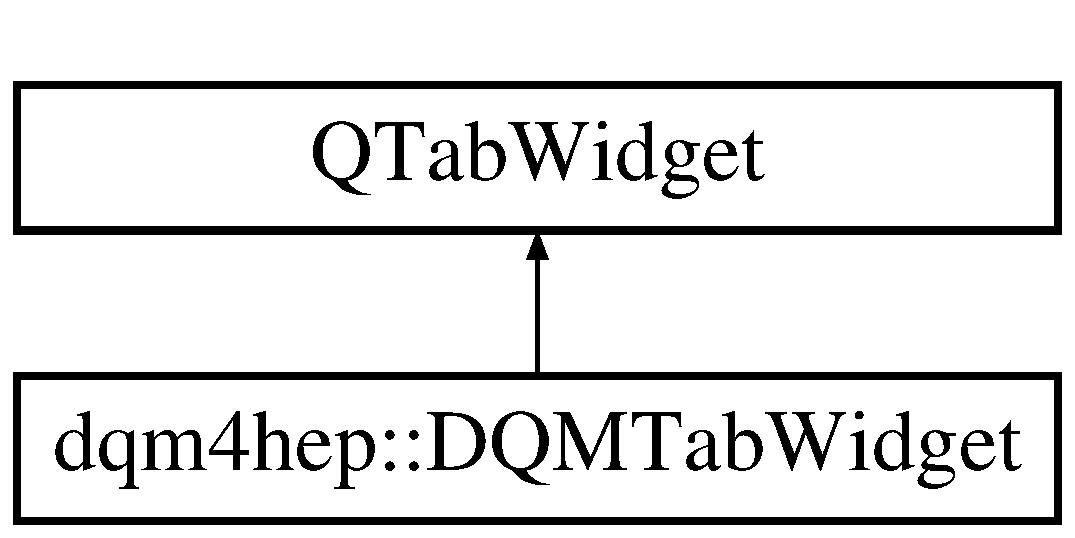
\includegraphics[height=2.000000cm]{classdqm4hep_1_1DQMTabWidget}
\end{center}
\end{figure}
\subsection*{Public Member Functions}
\begin{DoxyCompactItemize}
\item 
{\bf D\+Q\+M\+Tab\+Widget} (Q\+Widget $\ast$p\+Parent=0)
\begin{DoxyCompactList}\small\item\em Constructor. \end{DoxyCompactList}\item 
Q\+Tab\+Bar $\ast$ {\bf tab\+Bar} () const 
\begin{DoxyCompactList}\small\item\em Get the tab bar. \end{DoxyCompactList}\end{DoxyCompactItemize}


\subsection{Detailed Description}
\doxyref{D\+Q\+M\+Tab\+Widget}{p.}{classdqm4hep_1_1DQMTabWidget} class. 

Definition at line 53 of file D\+Q\+M\+Canvas\+View.\+cc.



\subsection{Constructor \& Destructor Documentation}
\index{dqm4hep\+::\+D\+Q\+M\+Tab\+Widget@{dqm4hep\+::\+D\+Q\+M\+Tab\+Widget}!D\+Q\+M\+Tab\+Widget@{D\+Q\+M\+Tab\+Widget}}
\index{D\+Q\+M\+Tab\+Widget@{D\+Q\+M\+Tab\+Widget}!dqm4hep\+::\+D\+Q\+M\+Tab\+Widget@{dqm4hep\+::\+D\+Q\+M\+Tab\+Widget}}
\subsubsection[{D\+Q\+M\+Tab\+Widget}]{\setlength{\rightskip}{0pt plus 5cm}dqm4hep\+::\+D\+Q\+M\+Tab\+Widget\+::\+D\+Q\+M\+Tab\+Widget (
\begin{DoxyParamCaption}
\item[{Q\+Widget $\ast$}]{p\+Parent = {\ttfamily 0}}
\end{DoxyParamCaption}
)}\label{classdqm4hep_1_1DQMTabWidget_a201c540aa9757d2cec860d2da93d0cf4}


Constructor. 



Definition at line 68 of file D\+Q\+M\+Canvas\+View.\+cc.


\begin{DoxyCode}
69   : QTabWidget(pParent)
70 \{
71   \textcolor{comment}{/* nop */}
72 \}
\end{DoxyCode}


\subsection{Member Function Documentation}
\index{dqm4hep\+::\+D\+Q\+M\+Tab\+Widget@{dqm4hep\+::\+D\+Q\+M\+Tab\+Widget}!tab\+Bar@{tab\+Bar}}
\index{tab\+Bar@{tab\+Bar}!dqm4hep\+::\+D\+Q\+M\+Tab\+Widget@{dqm4hep\+::\+D\+Q\+M\+Tab\+Widget}}
\subsubsection[{tab\+Bar}]{\setlength{\rightskip}{0pt plus 5cm}Q\+Tab\+Bar $\ast$ dqm4hep\+::\+D\+Q\+M\+Tab\+Widget\+::tab\+Bar (
\begin{DoxyParamCaption}
{}
\end{DoxyParamCaption}
) const}\label{classdqm4hep_1_1DQMTabWidget_ab4fdfaaa6ded22bc663e52decd6e1c5b}


Get the tab bar. 



Definition at line 76 of file D\+Q\+M\+Canvas\+View.\+cc.



Referenced by dqm4hep\+::\+D\+Q\+M\+Canvas\+View\+::create\+Context\+Menu(), and dqm4hep\+::\+D\+Q\+M\+Canvas\+View\+::event\+Filter().


\begin{DoxyCode}
77 \{
78   \textcolor{keywordflow}{return} QTabWidget::tabBar();
79 \}
\end{DoxyCode}


The documentation for this class was generated from the following file\+:\begin{DoxyCompactItemize}
\item 
{\bf D\+Q\+M\+Canvas\+View.\+cc}\end{DoxyCompactItemize}

\section{dqm4hep\+:\+:Tree\+Widget\+Item Class Reference}
\label{classdqm4hep_1_1TreeWidgetItem}\index{dqm4hep\+::\+Tree\+Widget\+Item@{dqm4hep\+::\+Tree\+Widget\+Item}}
Inheritance diagram for dqm4hep\+:\+:Tree\+Widget\+Item\+:\begin{figure}[H]
\begin{center}
\leavevmode
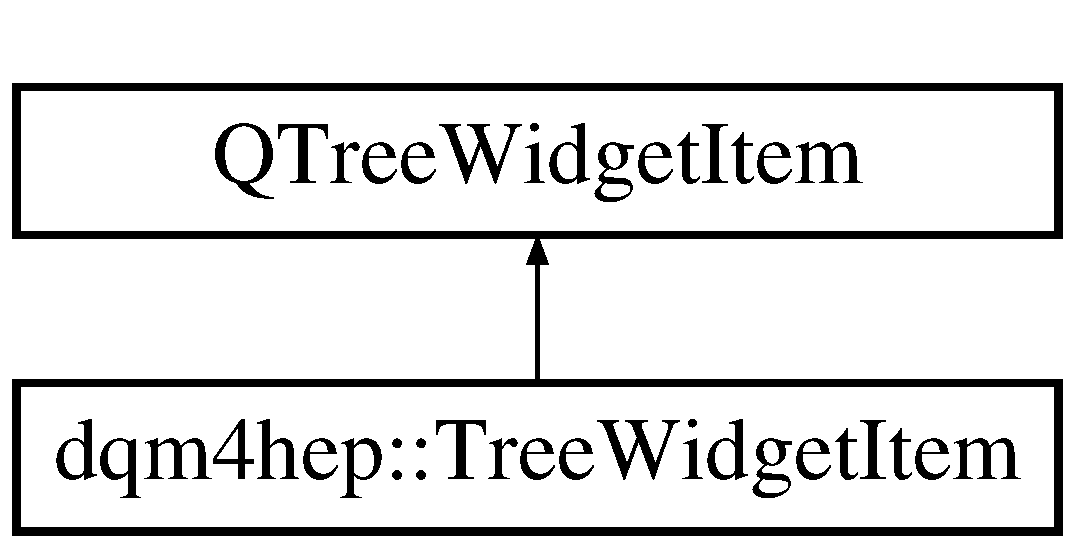
\includegraphics[height=2.000000cm]{classdqm4hep_1_1TreeWidgetItem}
\end{center}
\end{figure}
\subsection*{Public Member Functions}
\begin{DoxyCompactItemize}
\item 
{\bf Tree\+Widget\+Item} ()
\begin{DoxyCompactList}\small\item\em Constructor. \end{DoxyCompactList}\item 
{\bf Tree\+Widget\+Item} (Q\+Tree\+Widget\+Item $\ast$p\+Parent)
\begin{DoxyCompactList}\small\item\em Constructor with parent item. \end{DoxyCompactList}\item 
{\bf Tree\+Widget\+Item} (Q\+Tree\+Widget $\ast$p\+Tree\+Widget)
\begin{DoxyCompactList}\small\item\em Constructor with tree widget. \end{DoxyCompactList}\item 
void {\bf set\+Data} (int column, int role, const Q\+Variant \&value)
\begin{DoxyCompactList}\small\item\em Set data for a target column with a given role. \end{DoxyCompactList}\item 
void {\bf set\+Checkable} (bool checkable)
\begin{DoxyCompactList}\small\item\em Set whether the element can be checked (subscribed) \end{DoxyCompactList}\end{DoxyCompactItemize}
\subsection*{Private Attributes}
\begin{DoxyCompactItemize}
\item 
bool {\bf m\+\_\+checkable}
\end{DoxyCompactItemize}


\subsection{Detailed Description}


Definition at line 50 of file D\+Q\+M\+Monitor\+Element\+View.\+cc.



\subsection{Constructor \& Destructor Documentation}
\index{dqm4hep\+::\+Tree\+Widget\+Item@{dqm4hep\+::\+Tree\+Widget\+Item}!Tree\+Widget\+Item@{Tree\+Widget\+Item}}
\index{Tree\+Widget\+Item@{Tree\+Widget\+Item}!dqm4hep\+::\+Tree\+Widget\+Item@{dqm4hep\+::\+Tree\+Widget\+Item}}
\subsubsection[{Tree\+Widget\+Item}]{\setlength{\rightskip}{0pt plus 5cm}dqm4hep\+::\+Tree\+Widget\+Item\+::\+Tree\+Widget\+Item (
\begin{DoxyParamCaption}
{}
\end{DoxyParamCaption}
)}\label{classdqm4hep_1_1TreeWidgetItem_a294a20b55885a1222c729557507ab07c}


Constructor. 



Definition at line 79 of file D\+Q\+M\+Monitor\+Element\+View.\+cc.


\begin{DoxyCode}
79                                :
80     QTreeWidgetItem(),
81     m_checkable(\textcolor{keyword}{true})
82 \{
83   \textcolor{comment}{/* nop */}
84 \}
\end{DoxyCode}
\index{dqm4hep\+::\+Tree\+Widget\+Item@{dqm4hep\+::\+Tree\+Widget\+Item}!Tree\+Widget\+Item@{Tree\+Widget\+Item}}
\index{Tree\+Widget\+Item@{Tree\+Widget\+Item}!dqm4hep\+::\+Tree\+Widget\+Item@{dqm4hep\+::\+Tree\+Widget\+Item}}
\subsubsection[{Tree\+Widget\+Item}]{\setlength{\rightskip}{0pt plus 5cm}dqm4hep\+::\+Tree\+Widget\+Item\+::\+Tree\+Widget\+Item (
\begin{DoxyParamCaption}
\item[{Q\+Tree\+Widget\+Item $\ast$}]{p\+Parent}
\end{DoxyParamCaption}
)}\label{classdqm4hep_1_1TreeWidgetItem_a2912269b35cfc9d8a0fa14345d7ba5b0}


Constructor with parent item. 



Definition at line 88 of file D\+Q\+M\+Monitor\+Element\+View.\+cc.


\begin{DoxyCode}
88                                                        :
89     QTreeWidgetItem(pParent),
90     m_checkable(\textcolor{keyword}{true})
91 \{
92   \textcolor{comment}{/* nop */}
93 \}
\end{DoxyCode}
\index{dqm4hep\+::\+Tree\+Widget\+Item@{dqm4hep\+::\+Tree\+Widget\+Item}!Tree\+Widget\+Item@{Tree\+Widget\+Item}}
\index{Tree\+Widget\+Item@{Tree\+Widget\+Item}!dqm4hep\+::\+Tree\+Widget\+Item@{dqm4hep\+::\+Tree\+Widget\+Item}}
\subsubsection[{Tree\+Widget\+Item}]{\setlength{\rightskip}{0pt plus 5cm}dqm4hep\+::\+Tree\+Widget\+Item\+::\+Tree\+Widget\+Item (
\begin{DoxyParamCaption}
\item[{Q\+Tree\+Widget $\ast$}]{p\+Tree\+Widget}
\end{DoxyParamCaption}
)}\label{classdqm4hep_1_1TreeWidgetItem_a62257ba5240170c1c1b5f4e7e70b3c23}


Constructor with tree widget. 



Definition at line 97 of file D\+Q\+M\+Monitor\+Element\+View.\+cc.


\begin{DoxyCode}
97                                                        :
98     QTreeWidgetItem(pTreeWidget),
99     m_checkable(\textcolor{keyword}{true})
100 \{
101   \textcolor{comment}{/* nop */}
102 \}
\end{DoxyCode}


\subsection{Member Function Documentation}
\index{dqm4hep\+::\+Tree\+Widget\+Item@{dqm4hep\+::\+Tree\+Widget\+Item}!set\+Checkable@{set\+Checkable}}
\index{set\+Checkable@{set\+Checkable}!dqm4hep\+::\+Tree\+Widget\+Item@{dqm4hep\+::\+Tree\+Widget\+Item}}
\subsubsection[{set\+Checkable}]{\setlength{\rightskip}{0pt plus 5cm}void dqm4hep\+::\+Tree\+Widget\+Item\+::set\+Checkable (
\begin{DoxyParamCaption}
\item[{bool}]{checkable}
\end{DoxyParamCaption}
)}\label{classdqm4hep_1_1TreeWidgetItem_a733f5f8ad2cd3f3d71bec612ce2f3250}


Set whether the element can be checked (subscribed) 



Definition at line 168 of file D\+Q\+M\+Monitor\+Element\+View.\+cc.



References m\+\_\+checkable.



Referenced by dqm4hep\+::\+D\+Q\+M\+Monitor\+Element\+Navigator\+::add\+Monitor\+Element(), and dqm4hep\+::\+D\+Q\+M\+Monitor\+Element\+Navigator\+::enable\+Subscription().


\begin{DoxyCode}
169 \{
170   std::cout << \textcolor{stringliteral}{"Item "} << this->text(0).toStdString() << \textcolor{stringliteral}{" set checkable to "} << checkable << std::endl;
171   m_checkable = checkable;
172 \}
\end{DoxyCode}
\index{dqm4hep\+::\+Tree\+Widget\+Item@{dqm4hep\+::\+Tree\+Widget\+Item}!set\+Data@{set\+Data}}
\index{set\+Data@{set\+Data}!dqm4hep\+::\+Tree\+Widget\+Item@{dqm4hep\+::\+Tree\+Widget\+Item}}
\subsubsection[{set\+Data}]{\setlength{\rightskip}{0pt plus 5cm}void dqm4hep\+::\+Tree\+Widget\+Item\+::set\+Data (
\begin{DoxyParamCaption}
\item[{int}]{column, }
\item[{int}]{role, }
\item[{const Q\+Variant \&}]{value}
\end{DoxyParamCaption}
)}\label{classdqm4hep_1_1TreeWidgetItem_aa56dc3de3892457afe1e4ba05a63f6e5}


Set data for a target column with a given role. 



Definition at line 106 of file D\+Q\+M\+Monitor\+Element\+View.\+cc.



References dqm4hep\+::\+D\+Q\+M\+Monitor\+Element\+Navigator\+::get\+Collector\+Name(), dqm4hep\+::\+D\+Q\+M\+Monitoring\+::get\+Controller(), dqm4hep\+::\+D\+Q\+M\+Monitor\+Element\+Navigator\+::get\+Full\+Path\+Name(), dqm4hep\+::\+D\+Q\+M\+Monitor\+Element\+Navigator\+::get\+Module\+Name(), dqm4hep\+::\+D\+Q\+M\+Monitor\+Element\+Navigator\+::get\+Monitoring(), dqm4hep\+::\+D\+Q\+M\+Monitor\+Element\+Navigator\+::is\+Monitor\+Element\+Item(), dqm4hep\+::\+D\+Q\+M\+Monitoring\+Controller\+::log(), m\+\_\+checkable, dqm4hep\+::\+D\+Q\+M\+Monitoring\+Controller\+::subscribe(), and dqm4hep\+::\+D\+Q\+M\+Monitoring\+Controller\+::unsubscribe().



Referenced by dqm4hep\+::\+D\+Q\+M\+Monitor\+Element\+Navigator\+::add\+Monitor\+Element().


\begin{DoxyCode}
107 \{
108   \textcolor{keywordflow}{if}(0 == column && role == Qt::CheckStateRole)
109   \{
110     Qt::CheckState oldState = \textcolor{keyword}{static\_cast<}Qt::CheckState\textcolor{keyword}{>}(this->data(column, role).toInt());
111     Qt::CheckState newState = \textcolor{keyword}{static\_cast<}Qt::CheckState\textcolor{keyword}{>}(value.toInt());
112 
113     \textcolor{keywordflow}{if}(oldState == newState)
114     \{
115       QTreeWidgetItem::setData(column, role, value);
116       \textcolor{keywordflow}{return};
117     \}
118 
119     DQMMonitorElementNavigator *pNavigator = qobject\_cast<DQMMonitorElementNavigator *>(this->treeWidget())
      ;
120 
121     \textcolor{keywordflow}{if}(!pNavigator)
122     \{
123       QTreeWidgetItem::setData(column, role, value);
124       \textcolor{keywordflow}{return};
125     \}
126 
127     \textcolor{keywordflow}{if}(!pNavigator->isMonitorElementItem(\textcolor{keyword}{this}))
128     \{
129       QTreeWidgetItem::setData(column, role, value);
130       \textcolor{keywordflow}{return};
131     \}
132 
133     QString collectorName(pNavigator->getCollectorName());
134     QString moduleName(pNavigator->getModuleName(\textcolor{keyword}{this}));
135     QString fullPathName(pNavigator->getFullPathName(\textcolor{keyword}{this}));
136     QString monitorElementName(this->text(0));
137     std::string fullName = (DQMPath(fullPathName.toStdString()) + monitorElementName.toStdString()).getPath
      ();
138 
139 
140     DQMMonitorElementRequest request;
141     request.push\_back(DQMMonitorElementRequest::value\_type(moduleName.toStdString(), fullName));
142 
143     \textcolor{keywordflow}{if}(Qt::Checked == newState)
144     \{
145       \textcolor{keywordflow}{if}(m_checkable)
146       \{
147         std::cout << \textcolor{stringliteral}{"Subscribing to "} << fullName << std::endl;
148         pNavigator->getMonitoring()->getController()->subscribe(collectorName.toStdString(), request);
149       \}
150       \textcolor{keywordflow}{else}
151       \{
152         pNavigator->getMonitoring()->getController()->log(ERROR, \textcolor{stringliteral}{"Can't subscribe to monitor element to "} +
       fullName + \textcolor{stringliteral}{" (disabled)"});
153         \textcolor{keywordflow}{return};
154       \}
155     \}
156     \textcolor{keywordflow}{else}
157     \{
158       std::cout << \textcolor{stringliteral}{"Un-subscribing to "} << fullName << std::endl;
159       pNavigator->getMonitoring()->getController()->unsubscribe(collectorName.toStdString(), request);
160     \}
161   \}
162 
163   QTreeWidgetItem::setData(column, role, value);
164 \}
\end{DoxyCode}


\subsection{Member Data Documentation}
\index{dqm4hep\+::\+Tree\+Widget\+Item@{dqm4hep\+::\+Tree\+Widget\+Item}!m\+\_\+checkable@{m\+\_\+checkable}}
\index{m\+\_\+checkable@{m\+\_\+checkable}!dqm4hep\+::\+Tree\+Widget\+Item@{dqm4hep\+::\+Tree\+Widget\+Item}}
\subsubsection[{m\+\_\+checkable}]{\setlength{\rightskip}{0pt plus 5cm}bool dqm4hep\+::\+Tree\+Widget\+Item\+::m\+\_\+checkable\hspace{0.3cm}{\ttfamily [private]}}\label{classdqm4hep_1_1TreeWidgetItem_ab9bfc2a05189c9ef303da9d213d5dc1f}


Definition at line 74 of file D\+Q\+M\+Monitor\+Element\+View.\+cc.



Referenced by set\+Checkable(), and set\+Data().



The documentation for this class was generated from the following file\+:\begin{DoxyCompactItemize}
\item 
{\bf D\+Q\+M\+Monitor\+Element\+View.\+cc}\end{DoxyCompactItemize}

\chapter{File Documentation}
\section{D\+Q\+M\+Browser\+Widget.\+cc File Reference}
\label{DQMBrowserWidget_8cc}\index{D\+Q\+M\+Browser\+Widget.\+cc@{D\+Q\+M\+Browser\+Widget.\+cc}}
{\ttfamily \#include \char`\"{}dqm4hep/vis/\+D\+Q\+M\+Browser\+Widget.\+h\char`\"{}}\\*
{\ttfamily \#include \char`\"{}dqm4hep/vis/\+D\+Q\+M\+Monitoring.\+h\char`\"{}}\\*
{\ttfamily \#include \char`\"{}dqm4hep/vis/\+D\+Q\+M\+Monitoring\+Controller.\+h\char`\"{}}\\*
{\ttfamily \#include \char`\"{}dqm4hep/\+D\+Q\+M\+Network\+Tool.\+h\char`\"{}}\\*
{\ttfamily \#include \char`\"{}D\+Q\+M\+Viz\+Config.\+h\char`\"{}}\\*
{\ttfamily \#include $<$Q\+Combo\+Box$>$}\\*
{\ttfamily \#include $<$Q\+H\+Box\+Layout$>$}\\*
{\ttfamily \#include $<$Q\+V\+Box\+Layout$>$}\\*
{\ttfamily \#include $<$Q\+Line\+Edit$>$}\\*
{\ttfamily \#include $<$Q\+Group\+Box$>$}\\*
{\ttfamily \#include $<$Q\+Form\+Layout$>$}\\*
{\ttfamily \#include $<$Q\+Tree\+Widget$>$}\\*
{\ttfamily \#include $<$Q\+Push\+Button$>$}\\*
{\ttfamily \#include $<$Q\+Message\+Box$>$}\\*
{\ttfamily \#include $<$Q\+Label$>$}\\*
{\ttfamily \#include $<$Q\+Mutex\+Locker$>$}\\*
{\ttfamily \#include $<$Q\+List\+Widget$>$}\\*
{\ttfamily \#include $<$Q\+Header\+View$>$}\\*
{\ttfamily \#include \char`\"{}dic.\+hxx\char`\"{}}\\*
\subsection*{Namespaces}
\begin{DoxyCompactItemize}
\item 
 {\bf dqm4hep}
\end{DoxyCompactItemize}

\section{D\+Q\+M\+Browser\+Widget.\+h File Reference}
\label{DQMBrowserWidget_8h}\index{D\+Q\+M\+Browser\+Widget.\+h@{D\+Q\+M\+Browser\+Widget.\+h}}
{\ttfamily \#include \char`\"{}dqm4hep/\+D\+Q\+M4\+H\+E\+P.\+h\char`\"{}}\\*
{\ttfamily \#include \char`\"{}dqm4hep/vis/\+D\+Q\+M\+Gui\+Monitor\+Element\+Client.\+h\char`\"{}}\\*
{\ttfamily \#include $<$Q\+Widget$>$}\\*
{\ttfamily \#include $<$Q\+Group\+Box$>$}\\*
{\ttfamily \#include $<$Q\+Combo\+Box$>$}\\*
{\ttfamily \#include $<$Q\+Line\+Edit$>$}\\*
{\ttfamily \#include $<$Q\+Dialog$>$}\\*
{\ttfamily \#include $<$Q\+Mutex$>$}\\*
{\ttfamily \#include $<$Q\+Tree\+Widget$>$}\\*
{\ttfamily \#include $<$Q\+Key\+Event$>$}\\*
{\ttfamily \#include $<$Q\+Timer$>$}\\*
\subsection*{Classes}
\begin{DoxyCompactItemize}
\item 
class {\bf dqm4hep\+::\+D\+Q\+M\+Browser\+Widget}
\begin{DoxyCompactList}\small\item\em \doxyref{D\+Q\+M\+Browser\+Widget}{p.}{classdqm4hep_1_1DQMBrowserWidget} class. \end{DoxyCompactList}\end{DoxyCompactItemize}
\subsection*{Namespaces}
\begin{DoxyCompactItemize}
\item 
 {\bf dqm4hep}
\end{DoxyCompactItemize}

\section{D\+Q\+M\+Canvas.\+cc File Reference}
\label{DQMCanvas_8cc}\index{D\+Q\+M\+Canvas.\+cc@{D\+Q\+M\+Canvas.\+cc}}
{\ttfamily \#include \char`\"{}dqm4hep/vis/\+D\+Q\+M\+Canvas.\+h\char`\"{}}\\*
{\ttfamily \#include \char`\"{}dqm4hep/vis/\+D\+Q\+M\+Monitoring.\+h\char`\"{}}\\*
{\ttfamily \#include \char`\"{}dqm4hep/vis/\+D\+Q\+M\+Root\+Widget.\+h\char`\"{}}\\*
{\ttfamily \#include \char`\"{}dqm4hep/vis/\+D\+Q\+M\+Monitoring\+View.\+h\char`\"{}}\\*
\subsection*{Namespaces}
\begin{DoxyCompactItemize}
\item 
 {\bf dqm4hep}
\end{DoxyCompactItemize}

\section{D\+Q\+M\+Canvas.\+h File Reference}
\label{DQMCanvas_8h}\index{D\+Q\+M\+Canvas.\+h@{D\+Q\+M\+Canvas.\+h}}
{\ttfamily \#include $<$Q\+Mdi\+Sub\+Window$>$}\\*
{\ttfamily \#include $<$Q\+Close\+Event$>$}\\*
{\ttfamily \#include \char`\"{}dqm4hep/\+D\+Q\+M4\+H\+E\+P.\+h\char`\"{}}\\*
\subsection*{Classes}
\begin{DoxyCompactItemize}
\item 
class {\bf dqm4hep\+::\+D\+Q\+M\+Canvas}
\begin{DoxyCompactList}\small\item\em \doxyref{D\+Q\+M\+Canvas}{p.}{classdqm4hep_1_1DQMCanvas} class. \end{DoxyCompactList}\end{DoxyCompactItemize}
\subsection*{Namespaces}
\begin{DoxyCompactItemize}
\item 
 {\bf dqm4hep}
\end{DoxyCompactItemize}

\section{D\+Q\+M\+Canvas\+Area.\+cc File Reference}
\label{DQMCanvasArea_8cc}\index{D\+Q\+M\+Canvas\+Area.\+cc@{D\+Q\+M\+Canvas\+Area.\+cc}}
{\ttfamily \#include \char`\"{}dqm4hep/vis/\+D\+Q\+M\+Canvas\+Area.\+h\char`\"{}}\\*
{\ttfamily \#include \char`\"{}dqm4hep/vis/\+D\+Q\+M\+Monitoring.\+h\char`\"{}}\\*
{\ttfamily \#include \char`\"{}dqm4hep/vis/\+D\+Q\+M\+Monitoring\+View.\+h\char`\"{}}\\*
{\ttfamily \#include \char`\"{}dqm4hep/vis/\+D\+Q\+M\+Monitoring\+Model.\+h\char`\"{}}\\*
{\ttfamily \#include \char`\"{}dqm4hep/vis/\+D\+Q\+M\+Monitoring\+Controller.\+h\char`\"{}}\\*
{\ttfamily \#include \char`\"{}dqm4hep/vis/\+D\+Q\+M\+Canvas.\+h\char`\"{}}\\*
{\ttfamily \#include \char`\"{}dqm4hep/vis/\+D\+Q\+M\+Gui\+Monitor\+Element.\+h\char`\"{}}\\*
\subsection*{Namespaces}
\begin{DoxyCompactItemize}
\item 
 {\bf dqm4hep}
\end{DoxyCompactItemize}

\section{D\+Q\+M\+Canvas\+Area.\+h File Reference}
\label{DQMCanvasArea_8h}\index{D\+Q\+M\+Canvas\+Area.\+h@{D\+Q\+M\+Canvas\+Area.\+h}}
{\ttfamily \#include $<$Q\+Mdi\+Area$>$}\\*
\subsection*{Classes}
\begin{DoxyCompactItemize}
\item 
class {\bf dqm4hep\+::\+D\+Q\+M\+Canvas\+Area}
\begin{DoxyCompactList}\small\item\em \doxyref{D\+Q\+M\+Canvas\+Area}{p.}{classdqm4hep_1_1DQMCanvasArea} class. \end{DoxyCompactList}\end{DoxyCompactItemize}
\subsection*{Namespaces}
\begin{DoxyCompactItemize}
\item 
 {\bf dqm4hep}
\end{DoxyCompactItemize}

\section{D\+Q\+M\+Canvas\+View.\+cc File Reference}
\label{DQMCanvasView_8cc}\index{D\+Q\+M\+Canvas\+View.\+cc@{D\+Q\+M\+Canvas\+View.\+cc}}
{\ttfamily \#include \char`\"{}dqm4hep/vis/\+D\+Q\+M\+Canvas\+View.\+h\char`\"{}}\\*
{\ttfamily \#include \char`\"{}dqm4hep/\+D\+Q\+M\+Monitor\+Element.\+h\char`\"{}}\\*
{\ttfamily \#include \char`\"{}dqm4hep/vis/\+D\+Q\+M\+Monitoring.\+h\char`\"{}}\\*
{\ttfamily \#include \char`\"{}dqm4hep/vis/\+D\+Q\+M\+Monitoring\+View.\+h\char`\"{}}\\*
{\ttfamily \#include \char`\"{}dqm4hep/vis/\+D\+Q\+M\+Monitoring\+Controller.\+h\char`\"{}}\\*
{\ttfamily \#include \char`\"{}dqm4hep/vis/\+D\+Q\+M\+Monitoring\+Model.\+h\char`\"{}}\\*
{\ttfamily \#include \char`\"{}dqm4hep/vis/\+D\+Q\+M\+Canvas\+Area.\+h\char`\"{}}\\*
{\ttfamily \#include \char`\"{}dqm4hep/vis/\+D\+Q\+M\+Canvas.\+h\char`\"{}}\\*
{\ttfamily \#include \char`\"{}dqm4hep/vis/\+D\+Q\+M\+Gui\+Monitor\+Element.\+h\char`\"{}}\\*
{\ttfamily \#include $<$Q\+Action$>$}\\*
{\ttfamily \#include $<$Q\+Tab\+Bar$>$}\\*
{\ttfamily \#include $<$Q\+Input\+Dialog$>$}\\*
{\ttfamily \#include $<$Q\+String$>$}\\*
{\ttfamily \#include $<$Q\+Line\+Edit$>$}\\*
{\ttfamily \#include $<$Q\+Application$>$}\\*
{\ttfamily \#include $<$Q\+Tool\+Button$>$}\\*
{\ttfamily \#include $<$Q\+H\+Box\+Layout$>$}\\*
\subsection*{Classes}
\begin{DoxyCompactItemize}
\item 
class {\bf dqm4hep\+::\+D\+Q\+M\+Tab\+Widget}
\begin{DoxyCompactList}\small\item\em \doxyref{D\+Q\+M\+Tab\+Widget}{p.}{classdqm4hep_1_1DQMTabWidget} class. \end{DoxyCompactList}\end{DoxyCompactItemize}
\subsection*{Namespaces}
\begin{DoxyCompactItemize}
\item 
 {\bf dqm4hep}
\end{DoxyCompactItemize}

\section{D\+Q\+M\+Canvas\+View.\+h File Reference}
\label{DQMCanvasView_8h}\index{D\+Q\+M\+Canvas\+View.\+h@{D\+Q\+M\+Canvas\+View.\+h}}
{\ttfamily \#include \char`\"{}dqm4hep/\+D\+Q\+M4\+H\+E\+P.\+h\char`\"{}}\\*
{\ttfamily \#include \char`\"{}dqm4hep/\+D\+Q\+M\+Xml\+I\+O.\+h\char`\"{}}\\*
{\ttfamily \#include $<$Q\+Widget$>$}\\*
{\ttfamily \#include $<$Q\+Menu$>$}\\*
\subsection*{Classes}
\begin{DoxyCompactItemize}
\item 
class {\bf dqm4hep\+::\+D\+Q\+M\+Canvas\+View}
\begin{DoxyCompactList}\small\item\em \doxyref{D\+Q\+M\+Canvas\+View}{p.}{classdqm4hep_1_1DQMCanvasView} class. \end{DoxyCompactList}\end{DoxyCompactItemize}
\subsection*{Namespaces}
\begin{DoxyCompactItemize}
\item 
 {\bf dqm4hep}
\end{DoxyCompactItemize}

\section{D\+Q\+M\+Delete\+Later\+Object.\+h File Reference}
\label{DQMDeleteLaterObject_8h}\index{D\+Q\+M\+Delete\+Later\+Object.\+h@{D\+Q\+M\+Delete\+Later\+Object.\+h}}
{\ttfamily \#include $<$Q\+Object$>$}\\*
\subsection*{Classes}
\begin{DoxyCompactItemize}
\item 
class {\bf dqm4hep\+::\+D\+Q\+M\+Delete\+Later\+Object$<$ T $>$}
\begin{DoxyCompactList}\small\item\em \doxyref{D\+Q\+M\+Delete\+Later\+Object}{p.}{classdqm4hep_1_1DQMDeleteLaterObject} class. \end{DoxyCompactList}\end{DoxyCompactItemize}
\subsection*{Namespaces}
\begin{DoxyCompactItemize}
\item 
 {\bf dqm4hep}
\end{DoxyCompactItemize}

\section{D\+Q\+M\+Gui\+Monitor\+Element.\+cc File Reference}
\label{DQMGuiMonitorElement_8cc}\index{D\+Q\+M\+Gui\+Monitor\+Element.\+cc@{D\+Q\+M\+Gui\+Monitor\+Element.\+cc}}
{\ttfamily \#include \char`\"{}dqm4hep/vis/\+D\+Q\+M\+Gui\+Monitor\+Element.\+h\char`\"{}}\\*
{\ttfamily \#include \char`\"{}dqm4hep/\+D\+Q\+M\+Monitor\+Element.\+h\char`\"{}}\\*
{\ttfamily \#include \char`\"{}dqm4hep/vis/\+D\+Q\+M\+Gui\+Monitor\+Element\+Client.\+h\char`\"{}}\\*
{\ttfamily \#include \char`\"{}dqm4hep/vis/\+D\+Q\+M\+Monitoring.\+h\char`\"{}}\\*
\subsection*{Namespaces}
\begin{DoxyCompactItemize}
\item 
 {\bf dqm4hep}
\end{DoxyCompactItemize}

\section{D\+Q\+M\+Gui\+Monitor\+Element.\+h File Reference}
\label{DQMGuiMonitorElement_8h}\index{D\+Q\+M\+Gui\+Monitor\+Element.\+h@{D\+Q\+M\+Gui\+Monitor\+Element.\+h}}
{\ttfamily \#include $<$Q\+Object$>$}\\*
{\ttfamily \#include \char`\"{}dqm4hep/\+D\+Q\+M4\+H\+E\+P.\+h\char`\"{}}\\*
\subsection*{Classes}
\begin{DoxyCompactItemize}
\item 
class {\bf dqm4hep\+::\+D\+Q\+M\+Gui\+Monitor\+Element}
\begin{DoxyCompactList}\small\item\em \doxyref{D\+Q\+M\+Gui\+Monitor\+Element}{p.}{classdqm4hep_1_1DQMGuiMonitorElement} class. \end{DoxyCompactList}\end{DoxyCompactItemize}
\subsection*{Namespaces}
\begin{DoxyCompactItemize}
\item 
 {\bf dqm4hep}
\end{DoxyCompactItemize}
\subsection*{Typedefs}
\begin{DoxyCompactItemize}
\item 
typedef std\+::vector\\*
$<$ D\+Q\+M\+Gui\+Monitor\+Element $\ast$ $>$ {\bf dqm4hep\+::\+D\+Q\+M\+Gui\+Monitor\+Element\+List}
\end{DoxyCompactItemize}

\section{D\+Q\+M\+Gui\+Monitor\+Element\+Client.\+cc File Reference}
\label{DQMGuiMonitorElementClient_8cc}\index{D\+Q\+M\+Gui\+Monitor\+Element\+Client.\+cc@{D\+Q\+M\+Gui\+Monitor\+Element\+Client.\+cc}}
{\ttfamily \#include \char`\"{}dqm4hep/vis/\+D\+Q\+M\+Gui\+Monitor\+Element\+Client.\+h\char`\"{}}\\*
\subsection*{Namespaces}
\begin{DoxyCompactItemize}
\item 
 {\bf dqm4hep}
\end{DoxyCompactItemize}

\section{D\+Q\+M\+Gui\+Monitor\+Element\+Client.\+h File Reference}
\label{DQMGuiMonitorElementClient_8h}\index{D\+Q\+M\+Gui\+Monitor\+Element\+Client.\+h@{D\+Q\+M\+Gui\+Monitor\+Element\+Client.\+h}}
{\ttfamily \#include \char`\"{}dqm4hep/\+D\+Q\+M\+Messaging.\+h\char`\"{}}\\*
{\ttfamily \#include \char`\"{}dqm4hep/\+D\+Q\+M\+Monitor\+Element\+Client.\+h\char`\"{}}\\*
{\ttfamily \#include $<$Q\+Object$>$}\\*
\subsection*{Classes}
\begin{DoxyCompactItemize}
\item 
class {\bf dqm4hep\+::\+D\+Q\+M\+Gui\+Monitor\+Element\+Client}
\begin{DoxyCompactList}\small\item\em \doxyref{D\+Q\+M\+Gui\+Monitor\+Element\+Client}{p.}{classdqm4hep_1_1DQMGuiMonitorElementClient} class. \end{DoxyCompactList}\end{DoxyCompactItemize}
\subsection*{Namespaces}
\begin{DoxyCompactItemize}
\item 
 {\bf dqm4hep}
\end{DoxyCompactItemize}

\section{D\+Q\+M\+Job\+Interface.\+cc File Reference}
\label{DQMJobInterface_8cc}\index{D\+Q\+M\+Job\+Interface.\+cc@{D\+Q\+M\+Job\+Interface.\+cc}}
{\ttfamily \#include \char`\"{}dqm4hep/vis/\+D\+Q\+M\+Job\+Interface.\+h\char`\"{}}\\*
\subsection*{Namespaces}
\begin{DoxyCompactItemize}
\item 
 {\bf dqm4hep}
\end{DoxyCompactItemize}

\section{D\+Q\+M\+Job\+Interface.\+h File Reference}
\label{DQMJobInterface_8h}\index{D\+Q\+M\+Job\+Interface.\+h@{D\+Q\+M\+Job\+Interface.\+h}}
{\ttfamily \#include \char`\"{}Dim\+Job\+Interface.\+h\char`\"{}}\\*
{\ttfamily \#include $<$Q\+Object$>$}\\*
\subsection*{Classes}
\begin{DoxyCompactItemize}
\item 
class {\bf dqm4hep\+::\+D\+Q\+M\+Job\+Interface}
\begin{DoxyCompactList}\small\item\em \doxyref{D\+Q\+M\+Job\+Interface}{p.}{classdqm4hep_1_1DQMJobInterface} class. \end{DoxyCompactList}\end{DoxyCompactItemize}
\subsection*{Namespaces}
\begin{DoxyCompactItemize}
\item 
 {\bf dqm4hep}
\end{DoxyCompactItemize}

\section{D\+Q\+M\+Job\+Interface\+Widget.\+cc File Reference}
\label{DQMJobInterfaceWidget_8cc}\index{D\+Q\+M\+Job\+Interface\+Widget.\+cc@{D\+Q\+M\+Job\+Interface\+Widget.\+cc}}
{\ttfamily \#include \char`\"{}dqm4hep/vis/\+D\+Q\+M\+Job\+Interface\+Widget.\+h\char`\"{}}\\*
{\ttfamily \#include \char`\"{}dqm4hep/vis/\+D\+Q\+M\+Job\+Interface.\+h\char`\"{}}\\*
{\ttfamily \#include \char`\"{}D\+Q\+M\+Viz\+Config.\+h\char`\"{}}\\*
{\ttfamily \#include $<$Q\+Menu$>$}\\*
{\ttfamily \#include $<$Q\+Menu\+Bar$>$}\\*
{\ttfamily \#include $<$Q\+Action$>$}\\*
{\ttfamily \#include $<$Q\+Widget$>$}\\*
{\ttfamily \#include $<$Q\+Application$>$}\\*
{\ttfamily \#include $<$Q\+Splitter$>$}\\*
{\ttfamily \#include $<$Q\+Message\+Box$>$}\\*
{\ttfamily \#include $<$Q\+File\+Dialog$>$}\\*
{\ttfamily \#include $<$Q\+Input\+Dialog$>$}\\*
{\ttfamily \#include $<$Q\+V\+Box\+Layout$>$}\\*
{\ttfamily \#include $<$Q\+H\+Box\+Layout$>$}\\*
{\ttfamily \#include $<$Q\+Form\+Layout$>$}\\*
{\ttfamily \#include $<$Q\+Group\+Box$>$}\\*
{\ttfamily \#include $<$Q\+Header\+View$>$}\\*
{\ttfamily \#include $<$Q\+Context\+Menu\+Event$>$}\\*
\subsection*{Namespaces}
\begin{DoxyCompactItemize}
\item 
 {\bf dqm4hep}
\end{DoxyCompactItemize}

\section{D\+Q\+M\+Job\+Interface\+Widget.\+h File Reference}
\label{DQMJobInterfaceWidget_8h}\index{D\+Q\+M\+Job\+Interface\+Widget.\+h@{D\+Q\+M\+Job\+Interface\+Widget.\+h}}
{\ttfamily \#include \char`\"{}dqm4hep/\+D\+Q\+M4\+H\+E\+P.\+h\char`\"{}}\\*
{\ttfamily \#include $<$Q\+Widget$>$}\\*
{\ttfamily \#include $<$Q\+Combo\+Box$>$}\\*
{\ttfamily \#include $<$Q\+Label$>$}\\*
{\ttfamily \#include $<$Q\+Tree\+Widget$>$}\\*
{\ttfamily \#include $<$Q\+Push\+Button$>$}\\*
{\ttfamily \#include $<$Q\+Main\+Window$>$}\\*
{\ttfamily \#include $<$Q\+Spin\+Box$>$}\\*
{\ttfamily \#include \char`\"{}json/json.\+h\char`\"{}}\\*
\subsection*{Classes}
\begin{DoxyCompactItemize}
\item 
class {\bf dqm4hep\+::\+D\+Q\+M\+Job\+Interface\+Widget}
\begin{DoxyCompactList}\small\item\em \doxyref{D\+Q\+M\+Job\+Interface\+Widget}{p.}{classdqm4hep_1_1DQMJobInterfaceWidget} class. \end{DoxyCompactList}\end{DoxyCompactItemize}
\subsection*{Namespaces}
\begin{DoxyCompactItemize}
\item 
 {\bf dqm4hep}
\end{DoxyCompactItemize}

\section{D\+Q\+M\+Logger\+Widget.\+cc File Reference}
\label{DQMLoggerWidget_8cc}\index{D\+Q\+M\+Logger\+Widget.\+cc@{D\+Q\+M\+Logger\+Widget.\+cc}}
{\ttfamily \#include \char`\"{}dqm4hep/vis/\+D\+Q\+M\+Logger\+Widget.\+h\char`\"{}}\\*
{\ttfamily \#include $<$Q\+H\+Box\+Layout$>$}\\*
{\ttfamily \#include $<$Q\+Scroll\+Bar$>$}\\*
\subsection*{Namespaces}
\begin{DoxyCompactItemize}
\item 
 {\bf dqm4hep}
\end{DoxyCompactItemize}

\section{D\+Q\+M\+Logger\+Widget.\+h File Reference}
\label{DQMLoggerWidget_8h}\index{D\+Q\+M\+Logger\+Widget.\+h@{D\+Q\+M\+Logger\+Widget.\+h}}
{\ttfamily \#include \char`\"{}dqm4hep/\+D\+Q\+M4\+H\+E\+P.\+h\char`\"{}}\\*
{\ttfamily \#include \char`\"{}dqm4hep/\+D\+Q\+M\+Logger.\+h\char`\"{}}\\*
{\ttfamily \#include $<$Q\+Group\+Box$>$}\\*
{\ttfamily \#include $<$Q\+Color$>$}\\*
{\ttfamily \#include $<$Q\+Text\+Edit$>$}\\*
\subsection*{Classes}
\begin{DoxyCompactItemize}
\item 
class {\bf dqm4hep\+::\+D\+Q\+M\+Logger\+Widget}
\begin{DoxyCompactList}\small\item\em \doxyref{D\+Q\+M\+Logger\+Widget}{p.}{classdqm4hep_1_1DQMLoggerWidget} class. \end{DoxyCompactList}\end{DoxyCompactItemize}
\subsection*{Namespaces}
\begin{DoxyCompactItemize}
\item 
 {\bf dqm4hep}
\end{DoxyCompactItemize}

\section{D\+Q\+M\+Monitor\+Element\+Info\+Widget.\+cc File Reference}
\label{DQMMonitorElementInfoWidget_8cc}\index{D\+Q\+M\+Monitor\+Element\+Info\+Widget.\+cc@{D\+Q\+M\+Monitor\+Element\+Info\+Widget.\+cc}}
{\ttfamily \#include \char`\"{}dqm4hep/vis/\+D\+Q\+M\+Monitor\+Element\+Info\+Widget.\+h\char`\"{}}\\*
\subsection*{Namespaces}
\begin{DoxyCompactItemize}
\item 
 {\bf dqm4hep}
\end{DoxyCompactItemize}

\section{D\+Q\+M\+Monitor\+Element\+Info\+Widget.\+h File Reference}
\label{DQMMonitorElementInfoWidget_8h}\index{D\+Q\+M\+Monitor\+Element\+Info\+Widget.\+h@{D\+Q\+M\+Monitor\+Element\+Info\+Widget.\+h}}
{\ttfamily \#include $<$Q\+Widget$>$}\\*
{\ttfamily \#include $<$Q\+Check\+Box$>$}\\*
{\ttfamily \#include $<$Q\+Label$>$}\\*
{\ttfamily \#include $<$Q\+Text\+Edit$>$}\\*
{\ttfamily \#include $<$Q\+Group\+Box$>$}\\*
{\ttfamily \#include $<$Q\+Combo\+Box$>$}\\*
{\ttfamily \#include $<$Q\+H\+Box\+Layout$>$}\\*
{\ttfamily \#include $<$Q\+V\+Box\+Layout$>$}\\*
{\ttfamily \#include $<$Q\+Form\+Layout$>$}\\*
{\ttfamily \#include \char`\"{}dqm4hep/\+D\+Q\+M4\+H\+E\+P.\+h\char`\"{}}\\*
{\ttfamily \#include \char`\"{}dqm4hep/\+D\+Q\+M\+Monitor\+Element.\+h\char`\"{}}\\*
{\ttfamily \#include \char`\"{}dqm4hep/\+D\+Q\+M\+Quality\+Test.\+h\char`\"{}}\\*
{\ttfamily \#include \char`\"{}dqm4hep/vis/\+D\+Q\+M\+Gui\+Monitor\+Element.\+h\char`\"{}}\\*
\subsection*{Classes}
\begin{DoxyCompactItemize}
\item 
class {\bf dqm4hep\+::\+D\+Q\+M\+Monitor\+Element\+Info\+Widget}
\begin{DoxyCompactList}\small\item\em \doxyref{D\+Q\+M\+Monitor\+Element\+Info\+Widget}{p.}{classdqm4hep_1_1DQMMonitorElementInfoWidget} class. \end{DoxyCompactList}\end{DoxyCompactItemize}
\subsection*{Namespaces}
\begin{DoxyCompactItemize}
\item 
 {\bf dqm4hep}
\end{DoxyCompactItemize}

\section{D\+Q\+M\+Monitor\+Element\+View.\+cc File Reference}
\label{DQMMonitorElementView_8cc}\index{D\+Q\+M\+Monitor\+Element\+View.\+cc@{D\+Q\+M\+Monitor\+Element\+View.\+cc}}
{\ttfamily \#include \char`\"{}dqm4hep/vis/\+D\+Q\+M\+Monitor\+Element\+View.\+h\char`\"{}}\\*
{\ttfamily \#include \char`\"{}dqm4hep/vis/\+D\+Q\+M\+Monitoring.\+h\char`\"{}}\\*
{\ttfamily \#include \char`\"{}dqm4hep/vis/\+D\+Q\+M\+Monitoring\+Controller.\+h\char`\"{}}\\*
{\ttfamily \#include \char`\"{}dqm4hep/vis/\+D\+Q\+M\+Monitoring\+View.\+h\char`\"{}}\\*
{\ttfamily \#include \char`\"{}dqm4hep/vis/\+D\+Q\+M\+Monitoring\+Model.\+h\char`\"{}}\\*
{\ttfamily \#include \char`\"{}dqm4hep/vis/\+D\+Q\+M\+Canvas\+View.\+h\char`\"{}}\\*
{\ttfamily \#include \char`\"{}dqm4hep/\+D\+Q\+M\+Monitor\+Element.\+h\char`\"{}}\\*
{\ttfamily \#include \char`\"{}dqm4hep/vis/\+D\+Q\+M\+Gui\+Monitor\+Element.\+h\char`\"{}}\\*
{\ttfamily \#include \char`\"{}dqm4hep/vis/\+D\+Q\+M\+Gui\+Monitor\+Element\+Client.\+h\char`\"{}}\\*
{\ttfamily \#include $<$Q\+V\+Box\+Layout$>$}\\*
{\ttfamily \#include $<$Q\+Menu$>$}\\*
{\ttfamily \#include $<$Q\+Key\+Event$>$}\\*
{\ttfamily \#include $<$Q\+Set$>$}\\*
{\ttfamily \#include $<$Q\+Common\+Style$>$}\\*
{\ttfamily \#include $<$Q\+Timer$>$}\\*
{\ttfamily \#include $<$Q\+Application$>$}\\*
\subsection*{Classes}
\begin{DoxyCompactItemize}
\item 
class {\bf dqm4hep\+::\+Tree\+Widget\+Item}
\end{DoxyCompactItemize}
\subsection*{Namespaces}
\begin{DoxyCompactItemize}
\item 
 {\bf dqm4hep}
\end{DoxyCompactItemize}

\section{D\+Q\+M\+Monitor\+Element\+View.\+h File Reference}
\label{DQMMonitorElementView_8h}\index{D\+Q\+M\+Monitor\+Element\+View.\+h@{D\+Q\+M\+Monitor\+Element\+View.\+h}}
{\ttfamily \#include $<$Q\+Widget$>$}\\*
{\ttfamily \#include $<$Q\+Tool\+Box$>$}\\*
{\ttfamily \#include $<$Q\+Tree\+Widget$>$}\\*
{\ttfamily \#include \char`\"{}dqm4hep/\+D\+Q\+M4\+H\+E\+P.\+h\char`\"{}}\\*
{\ttfamily \#include \char`\"{}dqm4hep/\+D\+Q\+M\+Xml\+I\+O.\+h\char`\"{}}\\*
{\ttfamily \#include \char`\"{}dqm4hep/vis/\+D\+Q\+M\+Gui\+Monitor\+Element.\+h\char`\"{}}\\*
\subsection*{Classes}
\begin{DoxyCompactItemize}
\item 
class {\bf dqm4hep\+::\+D\+Q\+M\+Monitor\+Element\+Navigator}
\begin{DoxyCompactList}\small\item\em \doxyref{D\+Q\+M\+Monitor\+Element\+Navigator}{p.}{classdqm4hep_1_1DQMMonitorElementNavigator} class. \end{DoxyCompactList}\item 
class {\bf dqm4hep\+::\+D\+Q\+M\+Monitor\+Element\+View}
\begin{DoxyCompactList}\small\item\em \doxyref{D\+Q\+M\+Monitor\+Element\+View}{p.}{classdqm4hep_1_1DQMMonitorElementView} class. \end{DoxyCompactList}\end{DoxyCompactItemize}
\subsection*{Namespaces}
\begin{DoxyCompactItemize}
\item 
 {\bf dqm4hep}
\end{DoxyCompactItemize}

\section{D\+Q\+M\+Monitoring.\+cc File Reference}
\label{DQMMonitoring_8cc}\index{D\+Q\+M\+Monitoring.\+cc@{D\+Q\+M\+Monitoring.\+cc}}
{\ttfamily \#include \char`\"{}dqm4hep/vis/\+D\+Q\+M\+Monitoring.\+h\char`\"{}}\\*
{\ttfamily \#include \char`\"{}dqm4hep/vis/\+D\+Q\+M\+Monitoring\+Controller.\+h\char`\"{}}\\*
{\ttfamily \#include \char`\"{}dqm4hep/vis/\+D\+Q\+M\+Monitoring\+Model.\+h\char`\"{}}\\*
{\ttfamily \#include \char`\"{}dqm4hep/vis/\+D\+Q\+M\+Monitoring\+View.\+h\char`\"{}}\\*
\subsection*{Namespaces}
\begin{DoxyCompactItemize}
\item 
 {\bf dqm4hep}
\end{DoxyCompactItemize}

\section{D\+Q\+M\+Monitoring.\+h File Reference}
\label{DQMMonitoring_8h}\index{D\+Q\+M\+Monitoring.\+h@{D\+Q\+M\+Monitoring.\+h}}
{\ttfamily \#include \char`\"{}dqm4hep/\+D\+Q\+M4\+H\+E\+P.\+h\char`\"{}}\\*
\subsection*{Classes}
\begin{DoxyCompactItemize}
\item 
class {\bf dqm4hep\+::\+D\+Q\+M\+Monitoring}
\begin{DoxyCompactList}\small\item\em \doxyref{D\+Q\+M\+Monitoring}{p.}{classdqm4hep_1_1DQMMonitoring} class. \end{DoxyCompactList}\end{DoxyCompactItemize}
\subsection*{Namespaces}
\begin{DoxyCompactItemize}
\item 
 {\bf dqm4hep}
\end{DoxyCompactItemize}

\section{D\+Q\+M\+Monitoring\+Controller.\+cc File Reference}
\label{DQMMonitoringController_8cc}\index{D\+Q\+M\+Monitoring\+Controller.\+cc@{D\+Q\+M\+Monitoring\+Controller.\+cc}}
{\ttfamily \#include \char`\"{}dqm4hep/vis/\+D\+Q\+M\+Monitoring\+Controller.\+h\char`\"{}}\\*
{\ttfamily \#include \char`\"{}dqm4hep/vis/\+D\+Q\+M\+Monitoring.\+h\char`\"{}}\\*
{\ttfamily \#include \char`\"{}dqm4hep/vis/\+D\+Q\+M\+Monitoring\+View.\+h\char`\"{}}\\*
{\ttfamily \#include \char`\"{}dqm4hep/vis/\+D\+Q\+M\+Monitor\+Element\+View.\+h\char`\"{}}\\*
{\ttfamily \#include \char`\"{}dqm4hep/vis/\+D\+Q\+M\+Monitoring\+Model.\+h\char`\"{}}\\*
{\ttfamily \#include \char`\"{}dqm4hep/vis/\+D\+Q\+M\+Gui\+Monitor\+Element\+Client.\+h\char`\"{}}\\*
{\ttfamily \#include \char`\"{}dqm4hep/vis/\+D\+Q\+M\+Canvas.\+h\char`\"{}}\\*
{\ttfamily \#include \char`\"{}dqm4hep/vis/\+D\+Q\+M\+Root\+Widget.\+h\char`\"{}}\\*
{\ttfamily \#include \char`\"{}dqm4hep/vis/\+D\+Q\+M\+Canvas\+Area.\+h\char`\"{}}\\*
{\ttfamily \#include \char`\"{}dqm4hep/vis/\+D\+Q\+M\+Browser\+Widget.\+h\char`\"{}}\\*
{\ttfamily \#include \char`\"{}dqm4hep/vis/\+D\+Q\+M\+Monitor\+Element\+Info\+Widget.\+h\char`\"{}}\\*
{\ttfamily \#include \char`\"{}dqm4hep/\+D\+Q\+M\+Monitor\+Element.\+h\char`\"{}}\\*
{\ttfamily \#include \char`\"{}dqm4hep/\+D\+Q\+M\+Messaging.\+h\char`\"{}}\\*
{\ttfamily \#include \char`\"{}D\+Q\+M\+Core\+Config.\+h\char`\"{}}\\*
{\ttfamily \#include \char`\"{}D\+Q\+M\+Viz\+Config.\+h\char`\"{}}\\*
{\ttfamily \#include $<$Q\+Map$>$}\\*
{\ttfamily \#include $<$Q\+Dir$>$}\\*
{\ttfamily \#include $<$Q\+Desktop\+Services$>$}\\*
{\ttfamily \#include $<$Q\+Url$>$}\\*
{\ttfamily \#include $<$Q\+Message\+Box$>$}\\*
{\ttfamily \#include $<$Q\+Status\+Bar$>$}\\*
{\ttfamily \#include $<$Q\+Main\+Window$>$}\\*
{\ttfamily \#include $<$Q\+File\+Dialog$>$}\\*
{\ttfamily \#include $<$Q\+Application$>$}\\*
{\ttfamily \#include $<$T\+File.\+h$>$}\\*
{\ttfamily \#include $<$T\+Canvas.\+h$>$}\\*
{\ttfamily \#include $<$T\+H1.\+h$>$}\\*
{\ttfamily \#include $<$unistd.\+h$>$}\\*
{\ttfamily \#include $<$errno.\+h$>$}\\*
\subsection*{Namespaces}
\begin{DoxyCompactItemize}
\item 
 {\bf dqm4hep}
\end{DoxyCompactItemize}

\section{D\+Q\+M\+Monitoring\+Controller.\+h File Reference}
\label{DQMMonitoringController_8h}\index{D\+Q\+M\+Monitoring\+Controller.\+h@{D\+Q\+M\+Monitoring\+Controller.\+h}}
{\ttfamily \#include $<$Q\+Object$>$}\\*
{\ttfamily \#include $<$Q\+Color$>$}\\*
{\ttfamily \#include $<$Q\+Map$>$}\\*
{\ttfamily \#include $<$Q\+Icon$>$}\\*
{\ttfamily \#include \char`\"{}dqm4hep/\+D\+Q\+M\+Logger.\+h\char`\"{}}\\*
{\ttfamily \#include \char`\"{}dqm4hep/vis/\+D\+Q\+M\+Gui\+Monitor\+Element.\+h\char`\"{}}\\*
{\ttfamily \#include \char`\"{}dqm4hep/\+D\+Q\+M\+Messaging.\+h\char`\"{}}\\*
\subsection*{Classes}
\begin{DoxyCompactItemize}
\item 
class {\bf dqm4hep\+::\+D\+Q\+M\+Monitoring\+Controller}
\begin{DoxyCompactList}\small\item\em \doxyref{D\+Q\+M\+Monitoring\+Controller}{p.}{classdqm4hep_1_1DQMMonitoringController} class. \end{DoxyCompactList}\end{DoxyCompactItemize}
\subsection*{Namespaces}
\begin{DoxyCompactItemize}
\item 
 {\bf dqm4hep}
\end{DoxyCompactItemize}

\section{D\+Q\+M\+Monitoring\+Model.\+cc File Reference}
\label{DQMMonitoringModel_8cc}\index{D\+Q\+M\+Monitoring\+Model.\+cc@{D\+Q\+M\+Monitoring\+Model.\+cc}}
{\ttfamily \#include \char`\"{}dqm4hep/vis/\+D\+Q\+M\+Monitoring\+Model.\+h\char`\"{}}\\*
{\ttfamily \#include \char`\"{}dqm4hep/vis/\+D\+Q\+M\+Monitoring.\+h\char`\"{}}\\*
{\ttfamily \#include \char`\"{}dqm4hep/vis/\+D\+Q\+M\+Monitoring\+View.\+h\char`\"{}}\\*
{\ttfamily \#include \char`\"{}dqm4hep/vis/\+D\+Q\+M\+Monitoring\+Controller.\+h\char`\"{}}\\*
{\ttfamily \#include \char`\"{}dqm4hep/vis/\+D\+Q\+M\+Monitor\+Element\+View.\+h\char`\"{}}\\*
{\ttfamily \#include \char`\"{}dqm4hep/vis/\+D\+Q\+M\+Gui\+Monitor\+Element.\+h\char`\"{}}\\*
{\ttfamily \#include \char`\"{}dqm4hep/vis/\+D\+Q\+M\+Gui\+Monitor\+Element\+Client.\+h\char`\"{}}\\*
{\ttfamily \#include \char`\"{}dqm4hep/vis/\+D\+Q\+M\+Delete\+Later\+Object.\+h\char`\"{}}\\*
{\ttfamily \#include \char`\"{}dqm4hep/\+D\+Q\+M\+Monitor\+Element.\+h\char`\"{}}\\*
{\ttfamily \#include $<$algorithm$>$}\\*
{\ttfamily \#include $<$Q\+Map$>$}\\*
\subsection*{Namespaces}
\begin{DoxyCompactItemize}
\item 
 {\bf dqm4hep}
\end{DoxyCompactItemize}

\section{D\+Q\+M\+Monitoring\+Model.\+h File Reference}
\label{DQMMonitoringModel_8h}\index{D\+Q\+M\+Monitoring\+Model.\+h@{D\+Q\+M\+Monitoring\+Model.\+h}}
{\ttfamily \#include $<$Q\+Object$>$}\\*
{\ttfamily \#include $<$Q\+Icon$>$}\\*
{\ttfamily \#include $<$Q\+Color$>$}\\*
{\ttfamily \#include \char`\"{}dqm4hep/\+D\+Q\+M4\+H\+E\+P.\+h\char`\"{}}\\*
{\ttfamily \#include \char`\"{}dqm4hep/\+D\+Q\+M\+Storage.\+h\char`\"{}}\\*
\subsection*{Classes}
\begin{DoxyCompactItemize}
\item 
class {\bf dqm4hep\+::\+D\+Q\+M\+Monitoring\+Model}
\begin{DoxyCompactList}\small\item\em \doxyref{D\+Q\+M\+Monitoring\+Model}{p.}{classdqm4hep_1_1DQMMonitoringModel} class. \end{DoxyCompactList}\end{DoxyCompactItemize}
\subsection*{Namespaces}
\begin{DoxyCompactItemize}
\item 
 {\bf dqm4hep}
\end{DoxyCompactItemize}

\section{D\+Q\+M\+Monitoring\+View.\+cc File Reference}
\label{DQMMonitoringView_8cc}\index{D\+Q\+M\+Monitoring\+View.\+cc@{D\+Q\+M\+Monitoring\+View.\+cc}}
{\ttfamily \#include \char`\"{}dqm4hep/vis/\+D\+Q\+M\+Monitoring\+View.\+h\char`\"{}}\\*
{\ttfamily \#include \char`\"{}dqm4hep/vis/\+D\+Q\+M\+Monitoring\+Controller.\+h\char`\"{}}\\*
{\ttfamily \#include \char`\"{}dqm4hep/vis/\+D\+Q\+M\+Monitoring\+Model.\+h\char`\"{}}\\*
{\ttfamily \#include \char`\"{}dqm4hep/vis/\+D\+Q\+M\+Monitoring.\+h\char`\"{}}\\*
{\ttfamily \#include \char`\"{}dqm4hep/vis/\+D\+Q\+M\+Monitor\+Element\+View.\+h\char`\"{}}\\*
{\ttfamily \#include \char`\"{}dqm4hep/vis/\+D\+Q\+M\+Canvas\+View.\+h\char`\"{}}\\*
{\ttfamily \#include \char`\"{}dqm4hep/\+D\+Q\+M\+Messaging.\+h\char`\"{}}\\*
{\ttfamily \#include \char`\"{}D\+Q\+M\+Core\+Config.\+h\char`\"{}}\\*
{\ttfamily \#include \char`\"{}D\+Q\+M\+Viz\+Config.\+h\char`\"{}}\\*
{\ttfamily \#include $<$Q\+Menu$>$}\\*
{\ttfamily \#include $<$Q\+V\+Box\+Layout$>$}\\*
{\ttfamily \#include $<$Q\+Action$>$}\\*
{\ttfamily \#include $<$Q\+Message\+Box$>$}\\*
{\ttfamily \#include $<$Q\+Dir$>$}\\*
{\ttfamily \#include $<$Q\+Icon$>$}\\*
{\ttfamily \#include $<$Q\+Url$>$}\\*
{\ttfamily \#include $<$Q\+Status\+Bar$>$}\\*
{\ttfamily \#include $<$Q\+Desktop\+Services$>$}\\*
{\ttfamily \#include $<$Q\+Application$>$}\\*
{\ttfamily \#include $<$Q\+Splitter$>$}\\*
{\ttfamily \#include $<$Q\+Menu\+Bar$>$}\\*
{\ttfamily \#include $<$Q\+File\+Dialog$>$}\\*
{\ttfamily \#include $<$Q\+Group\+Box$>$}\\*
{\ttfamily \#include $<$Q\+Push\+Button$>$}\\*
{\ttfamily \#include $<$Q\+Close\+Event$>$}\\*
\subsection*{Classes}
\begin{DoxyCompactItemize}
\item 
class {\bf dqm4hep\+::\+D\+Q\+M\+Monitoring\+Main\+Window}
\end{DoxyCompactItemize}
\subsection*{Namespaces}
\begin{DoxyCompactItemize}
\item 
 {\bf dqm4hep}
\end{DoxyCompactItemize}

\section{D\+Q\+M\+Monitoring\+View.\+h File Reference}
\label{DQMMonitoringView_8h}\index{D\+Q\+M\+Monitoring\+View.\+h@{D\+Q\+M\+Monitoring\+View.\+h}}
{\ttfamily \#include \char`\"{}dqm4hep/\+D\+Q\+M4\+H\+E\+P.\+h\char`\"{}}\\*
{\ttfamily \#include \char`\"{}dqm4hep/\+D\+Q\+M\+Xml\+I\+O.\+h\char`\"{}}\\*
{\ttfamily \#include $<$Q\+Object$>$}\\*
{\ttfamily \#include $<$Q\+Main\+Window$>$}\\*
\subsection*{Classes}
\begin{DoxyCompactItemize}
\item 
class {\bf dqm4hep\+::\+D\+Q\+M\+Monitoring\+View}
\begin{DoxyCompactList}\small\item\em \doxyref{D\+Q\+M\+Monitoring\+View}{p.}{classdqm4hep_1_1DQMMonitoringView} class. \end{DoxyCompactList}\end{DoxyCompactItemize}
\subsection*{Namespaces}
\begin{DoxyCompactItemize}
\item 
 {\bf dqm4hep}
\end{DoxyCompactItemize}

\section{D\+Q\+M\+Root\+Widget.\+cc File Reference}
\label{DQMRootWidget_8cc}\index{D\+Q\+M\+Root\+Widget.\+cc@{D\+Q\+M\+Root\+Widget.\+cc}}
{\ttfamily \#include \char`\"{}dqm4hep/vis/\+D\+Q\+M\+Root\+Widget.\+h\char`\"{}}\\*
{\ttfamily \#include \char`\"{}dqm4hep/vis/\+D\+Q\+M\+Canvas.\+h\char`\"{}}\\*
{\ttfamily \#include \char`\"{}dqm4hep/vis/\+D\+Q\+M\+Canvas\+Area.\+h\char`\"{}}\\*
{\ttfamily \#include \char`\"{}dqm4hep/vis/\+D\+Q\+M\+Canvas\+View.\+h\char`\"{}}\\*
{\ttfamily \#include \char`\"{}dqm4hep/vis/\+D\+Q\+M\+Monitoring.\+h\char`\"{}}\\*
{\ttfamily \#include \char`\"{}dqm4hep/vis/\+D\+Q\+M\+Monitoring\+Controller.\+h\char`\"{}}\\*
{\ttfamily \#include \char`\"{}dqm4hep/vis/\+D\+Q\+M\+Monitoring\+Model.\+h\char`\"{}}\\*
{\ttfamily \#include \char`\"{}dqm4hep/vis/\+D\+Q\+M\+Monitoring\+View.\+h\char`\"{}}\\*
{\ttfamily \#include \char`\"{}dqm4hep/\+D\+Q\+M\+Monitor\+Element.\+h\char`\"{}}\\*
{\ttfamily \#include \char`\"{}D\+Q\+M\+Core\+Config.\+h\char`\"{}}\\*
{\ttfamily \#include \char`\"{}D\+Q\+M\+Viz\+Config.\+h\char`\"{}}\\*
{\ttfamily \#include $<$T\+Image.\+h$>$}\\*
{\ttfamily \#include $<$T\+H1.\+h$>$}\\*
{\ttfamily \#include $<$Q\+Action$>$}\\*
{\ttfamily \#include $<$Q\+Application$>$}\\*
{\ttfamily \#include $<$Q\+Input\+Dialog$>$}\\*
\subsection*{Namespaces}
\begin{DoxyCompactItemize}
\item 
 {\bf dqm4hep}
\end{DoxyCompactItemize}

\section{D\+Q\+M\+Root\+Widget.\+h File Reference}
\label{DQMRootWidget_8h}\index{D\+Q\+M\+Root\+Widget.\+h@{D\+Q\+M\+Root\+Widget.\+h}}
{\ttfamily \#include $<$T\+Qt\+Widget.\+h$>$}\\*
{\ttfamily \#include $<$Q\+Menu$>$}\\*
{\ttfamily \#include \char`\"{}dqm4hep/vis/\+D\+Q\+M\+Gui\+Monitor\+Element.\+h\char`\"{}}\\*
\subsection*{Classes}
\begin{DoxyCompactItemize}
\item 
class {\bf dqm4hep\+::\+D\+Q\+M\+Root\+Widget}
\begin{DoxyCompactList}\small\item\em \doxyref{D\+Q\+M\+Root\+Widget}{p.}{classdqm4hep_1_1DQMRootWidget} class. \end{DoxyCompactList}\end{DoxyCompactItemize}
\subsection*{Namespaces}
\begin{DoxyCompactItemize}
\item 
 {\bf dqm4hep}
\end{DoxyCompactItemize}

\section{D\+Q\+M\+Run\+Control\+Widget.\+cc File Reference}
\label{DQMRunControlWidget_8cc}\index{D\+Q\+M\+Run\+Control\+Widget.\+cc@{D\+Q\+M\+Run\+Control\+Widget.\+cc}}
{\ttfamily \#include \char`\"{}dqm4hep/vis/\+D\+Q\+M\+Run\+Control\+Widget.\+h\char`\"{}}\\*
{\ttfamily \#include \char`\"{}dqm4hep/\+D\+Q\+M\+Run.\+h\char`\"{}}\\*
{\ttfamily \#include \char`\"{}dqm4hep/\+D\+Q\+M\+Core\+Tool.\+h\char`\"{}}\\*
{\ttfamily \#include \char`\"{}dqm4hep/\+D\+Q\+M\+Xml\+Helper.\+h\char`\"{}}\\*
{\ttfamily \#include \char`\"{}dqm4hep/tinyxml.\+h\char`\"{}}\\*
{\ttfamily \#include $<$Q\+V\+Box\+Layout$>$}\\*
{\ttfamily \#include $<$Q\+Form\+Layout$>$}\\*
{\ttfamily \#include $<$Q\+File\+Dialog$>$}\\*
{\ttfamily \#include $<$Q\+Message\+Box$>$}\\*
{\ttfamily \#include $<$fstream$>$}\\*
\subsection*{Namespaces}
\begin{DoxyCompactItemize}
\item 
 {\bf dqm4hep}
\end{DoxyCompactItemize}

\section{D\+Q\+M\+Run\+Control\+Widget.\+h File Reference}
\label{DQMRunControlWidget_8h}\index{D\+Q\+M\+Run\+Control\+Widget.\+h@{D\+Q\+M\+Run\+Control\+Widget.\+h}}
{\ttfamily \#include \char`\"{}dqm4hep/\+D\+Q\+M4\+H\+E\+P.\+h\char`\"{}}\\*
{\ttfamily \#include \char`\"{}dqm4hep/\+D\+Q\+M\+Logger.\+h\char`\"{}}\\*
{\ttfamily \#include \char`\"{}dqm4hep/\+D\+Q\+M\+Run\+Control\+Service.\+h\char`\"{}}\\*
{\ttfamily \#include $<$Q\+Group\+Box$>$}\\*
{\ttfamily \#include $<$Q\+Push\+Button$>$}\\*
{\ttfamily \#include $<$Q\+Spin\+Box$>$}\\*
{\ttfamily \#include $<$Q\+Line\+Edit$>$}\\*
{\ttfamily \#include $<$Q\+Text\+Edit$>$}\\*
{\ttfamily \#include $<$Q\+Table\+Widget$>$}\\*
{\ttfamily \#include $<$Q\+Header\+View$>$}\\*
{\ttfamily \#include $<$Q\+Label$>$}\\*
\subsection*{Classes}
\begin{DoxyCompactItemize}
\item 
class {\bf dqm4hep\+::\+D\+Q\+M\+Run\+Control\+Widget}
\begin{DoxyCompactList}\small\item\em \doxyref{D\+Q\+M\+Run\+Control\+Widget}{p.}{classdqm4hep_1_1DQMRunControlWidget} class. \end{DoxyCompactList}\end{DoxyCompactItemize}
\subsection*{Namespaces}
\begin{DoxyCompactItemize}
\item 
 {\bf dqm4hep}
\end{DoxyCompactItemize}

\section{D\+Q\+M\+Viz\+Config.\+h File Reference}
\label{DQMVizConfig_8h}\index{D\+Q\+M\+Viz\+Config.\+h@{D\+Q\+M\+Viz\+Config.\+h}}
\subsection*{Macros}
\begin{DoxyCompactItemize}
\item 
\#define {\bf D\+Q\+M\+Viz\+\_\+\+M\+A\+J\+O\+R\+\_\+\+V\+E\+R\+S\+I\+O\+N}~1
\item 
\#define {\bf D\+Q\+M\+Viz\+\_\+\+M\+I\+N\+O\+R\+\_\+\+V\+E\+R\+S\+I\+O\+N}~2
\item 
\#define {\bf D\+Q\+M\+Viz\+\_\+\+P\+A\+T\+C\+H\+\_\+\+L\+E\+V\+E\+L}~0
\item 
\#define {\bf D\+Q\+M\+Viz\+\_\+\+V\+E\+R\+S\+I\+O\+N\+\_\+\+S\+T\+R}~\char`\"{}1.\+2.\+0\char`\"{}
\item 
\#define {\bf D\+Q\+M\+Viz\+\_\+\+V\+E\+R\+S\+I\+O\+N\+\_\+\+G\+E}(M\+A\+J\+V, M\+I\+N\+V, P\+L\+E\+V)
\item 
\#define {\bf D\+Q\+M\+Viz\+\_\+\+D\+I\+R}~\char`\"{}/home/rete/soft/test/D\+Q\+M4\+H\+E\+P\char`\"{}
\end{DoxyCompactItemize}


\subsection{Macro Definition Documentation}
\index{D\+Q\+M\+Viz\+Config.\+h@{D\+Q\+M\+Viz\+Config.\+h}!D\+Q\+M\+Viz\+\_\+\+D\+I\+R@{D\+Q\+M\+Viz\+\_\+\+D\+I\+R}}
\index{D\+Q\+M\+Viz\+\_\+\+D\+I\+R@{D\+Q\+M\+Viz\+\_\+\+D\+I\+R}!D\+Q\+M\+Viz\+Config.\+h@{D\+Q\+M\+Viz\+Config.\+h}}
\subsubsection[{D\+Q\+M\+Viz\+\_\+\+D\+I\+R}]{\setlength{\rightskip}{0pt plus 5cm}\#define D\+Q\+M\+Viz\+\_\+\+D\+I\+R~\char`\"{}/home/rete/soft/test/D\+Q\+M4\+H\+E\+P\char`\"{}}\label{DQMVizConfig_8h_abf4bf4d374673b2ac8aede7c327e25b8}


Definition at line 15 of file D\+Q\+M\+Viz\+Config.\+h.



Referenced by dqm4hep\+::\+D\+Q\+M\+Monitoring\+Controller\+::about\+D\+Q\+M4\+H\+E\+P(), dqm4hep\+::\+D\+Q\+M\+Monitoring\+View\+::build\+View(), dqm4hep\+::\+D\+Q\+M\+Monitoring\+Controller\+::get\+Icon(), dqm4hep\+::\+D\+Q\+M\+Root\+Widget\+::get\+No\+Vis\+Image(), and dqm4hep\+::\+D\+Q\+M\+Monitoring\+Controller\+::open\+Browser().

\index{D\+Q\+M\+Viz\+Config.\+h@{D\+Q\+M\+Viz\+Config.\+h}!D\+Q\+M\+Viz\+\_\+\+M\+A\+J\+O\+R\+\_\+\+V\+E\+R\+S\+I\+O\+N@{D\+Q\+M\+Viz\+\_\+\+M\+A\+J\+O\+R\+\_\+\+V\+E\+R\+S\+I\+O\+N}}
\index{D\+Q\+M\+Viz\+\_\+\+M\+A\+J\+O\+R\+\_\+\+V\+E\+R\+S\+I\+O\+N@{D\+Q\+M\+Viz\+\_\+\+M\+A\+J\+O\+R\+\_\+\+V\+E\+R\+S\+I\+O\+N}!D\+Q\+M\+Viz\+Config.\+h@{D\+Q\+M\+Viz\+Config.\+h}}
\subsubsection[{D\+Q\+M\+Viz\+\_\+\+M\+A\+J\+O\+R\+\_\+\+V\+E\+R\+S\+I\+O\+N}]{\setlength{\rightskip}{0pt plus 5cm}\#define D\+Q\+M\+Viz\+\_\+\+M\+A\+J\+O\+R\+\_\+\+V\+E\+R\+S\+I\+O\+N~1}\label{DQMVizConfig_8h_ab7ddf2eaedb434af9fc582e8018e7103}


Definition at line 5 of file D\+Q\+M\+Viz\+Config.\+h.

\index{D\+Q\+M\+Viz\+Config.\+h@{D\+Q\+M\+Viz\+Config.\+h}!D\+Q\+M\+Viz\+\_\+\+M\+I\+N\+O\+R\+\_\+\+V\+E\+R\+S\+I\+O\+N@{D\+Q\+M\+Viz\+\_\+\+M\+I\+N\+O\+R\+\_\+\+V\+E\+R\+S\+I\+O\+N}}
\index{D\+Q\+M\+Viz\+\_\+\+M\+I\+N\+O\+R\+\_\+\+V\+E\+R\+S\+I\+O\+N@{D\+Q\+M\+Viz\+\_\+\+M\+I\+N\+O\+R\+\_\+\+V\+E\+R\+S\+I\+O\+N}!D\+Q\+M\+Viz\+Config.\+h@{D\+Q\+M\+Viz\+Config.\+h}}
\subsubsection[{D\+Q\+M\+Viz\+\_\+\+M\+I\+N\+O\+R\+\_\+\+V\+E\+R\+S\+I\+O\+N}]{\setlength{\rightskip}{0pt plus 5cm}\#define D\+Q\+M\+Viz\+\_\+\+M\+I\+N\+O\+R\+\_\+\+V\+E\+R\+S\+I\+O\+N~2}\label{DQMVizConfig_8h_af8857d60d07f072cbcee6ebcfda22fb4}


Definition at line 6 of file D\+Q\+M\+Viz\+Config.\+h.

\index{D\+Q\+M\+Viz\+Config.\+h@{D\+Q\+M\+Viz\+Config.\+h}!D\+Q\+M\+Viz\+\_\+\+P\+A\+T\+C\+H\+\_\+\+L\+E\+V\+E\+L@{D\+Q\+M\+Viz\+\_\+\+P\+A\+T\+C\+H\+\_\+\+L\+E\+V\+E\+L}}
\index{D\+Q\+M\+Viz\+\_\+\+P\+A\+T\+C\+H\+\_\+\+L\+E\+V\+E\+L@{D\+Q\+M\+Viz\+\_\+\+P\+A\+T\+C\+H\+\_\+\+L\+E\+V\+E\+L}!D\+Q\+M\+Viz\+Config.\+h@{D\+Q\+M\+Viz\+Config.\+h}}
\subsubsection[{D\+Q\+M\+Viz\+\_\+\+P\+A\+T\+C\+H\+\_\+\+L\+E\+V\+E\+L}]{\setlength{\rightskip}{0pt plus 5cm}\#define D\+Q\+M\+Viz\+\_\+\+P\+A\+T\+C\+H\+\_\+\+L\+E\+V\+E\+L~0}\label{DQMVizConfig_8h_aebee4fd069dbe0b0323c43f75afa495a}


Definition at line 7 of file D\+Q\+M\+Viz\+Config.\+h.

\index{D\+Q\+M\+Viz\+Config.\+h@{D\+Q\+M\+Viz\+Config.\+h}!D\+Q\+M\+Viz\+\_\+\+V\+E\+R\+S\+I\+O\+N\+\_\+\+G\+E@{D\+Q\+M\+Viz\+\_\+\+V\+E\+R\+S\+I\+O\+N\+\_\+\+G\+E}}
\index{D\+Q\+M\+Viz\+\_\+\+V\+E\+R\+S\+I\+O\+N\+\_\+\+G\+E@{D\+Q\+M\+Viz\+\_\+\+V\+E\+R\+S\+I\+O\+N\+\_\+\+G\+E}!D\+Q\+M\+Viz\+Config.\+h@{D\+Q\+M\+Viz\+Config.\+h}}
\subsubsection[{D\+Q\+M\+Viz\+\_\+\+V\+E\+R\+S\+I\+O\+N\+\_\+\+G\+E}]{\setlength{\rightskip}{0pt plus 5cm}\#define D\+Q\+M\+Viz\+\_\+\+V\+E\+R\+S\+I\+O\+N\+\_\+\+G\+E(
\begin{DoxyParamCaption}
\item[{}]{M\+A\+J\+V, }
\item[{}]{M\+I\+N\+V, }
\item[{}]{P\+L\+E\+V}
\end{DoxyParamCaption}
)}\label{DQMVizConfig_8h_ac246e60e832927749d74fd0fed7c1152}
{\bfseries Value\+:}
\begin{DoxyCode}
( (DQMViz_MAJOR_VERSION > MAJV) || ( (DQMViz_MAJOR_VERSION == MAJV) && (
      DQMViz_MINOR_VERSION > MINV) ) \(\backslash\)
  || ( (DQMViz_MAJOR_VERSION == MAJV) && (DQMViz_MINOR_VERSION == MINV) && (
      DQMViz_PATCH_LEVEL >= PLEV) ) )
\end{DoxyCode}


Definition at line 9 of file D\+Q\+M\+Viz\+Config.\+h.

\index{D\+Q\+M\+Viz\+Config.\+h@{D\+Q\+M\+Viz\+Config.\+h}!D\+Q\+M\+Viz\+\_\+\+V\+E\+R\+S\+I\+O\+N\+\_\+\+S\+T\+R@{D\+Q\+M\+Viz\+\_\+\+V\+E\+R\+S\+I\+O\+N\+\_\+\+S\+T\+R}}
\index{D\+Q\+M\+Viz\+\_\+\+V\+E\+R\+S\+I\+O\+N\+\_\+\+S\+T\+R@{D\+Q\+M\+Viz\+\_\+\+V\+E\+R\+S\+I\+O\+N\+\_\+\+S\+T\+R}!D\+Q\+M\+Viz\+Config.\+h@{D\+Q\+M\+Viz\+Config.\+h}}
\subsubsection[{D\+Q\+M\+Viz\+\_\+\+V\+E\+R\+S\+I\+O\+N\+\_\+\+S\+T\+R}]{\setlength{\rightskip}{0pt plus 5cm}\#define D\+Q\+M\+Viz\+\_\+\+V\+E\+R\+S\+I\+O\+N\+\_\+\+S\+T\+R~\char`\"{}1.\+2.\+0\char`\"{}}\label{DQMVizConfig_8h_aae888a39b8c6b48565681a49bd768e54}


Definition at line 8 of file D\+Q\+M\+Viz\+Config.\+h.



Referenced by dqm4hep\+::\+D\+Q\+M\+Monitoring\+Controller\+::about\+D\+Q\+M4\+H\+E\+P().


%--- End generated contents ---

% Index
\newpage
\phantomsection
\addcontentsline{toc}{chapter}{Index}
\printindex

\end{document}
